% Options for packages loaded elsewhere
\PassOptionsToPackage{unicode}{hyperref}
\PassOptionsToPackage{hyphens}{url}
%
\documentclass[
  letterpaper,
]{book}

\usepackage{amsmath,amssymb}
\usepackage{lmodern}
\usepackage{iftex}
\ifPDFTeX
  \usepackage[T1]{fontenc}
  \usepackage[utf8]{inputenc}
  \usepackage{textcomp} % provide euro and other symbols
\else % if luatex or xetex
  \usepackage{unicode-math}
  \defaultfontfeatures{Scale=MatchLowercase}
  \defaultfontfeatures[\rmfamily]{Ligatures=TeX,Scale=1}
  \setmainfont[]{Mont}
\fi
% Use upquote if available, for straight quotes in verbatim environments
\IfFileExists{upquote.sty}{\usepackage{upquote}}{}
\IfFileExists{microtype.sty}{% use microtype if available
  \usepackage[]{microtype}
  \UseMicrotypeSet[protrusion]{basicmath} % disable protrusion for tt fonts
}{}
\makeatletter
\@ifundefined{KOMAClassName}{% if non-KOMA class
  \IfFileExists{parskip.sty}{%
    \usepackage{parskip}
  }{% else
    \setlength{\parindent}{0pt}
    \setlength{\parskip}{6pt plus 2pt minus 1pt}}
}{% if KOMA class
  \KOMAoptions{parskip=half}}
\makeatother
\usepackage{xcolor}
\usepackage[normalem]{ulem}
\setlength{\emergencystretch}{3em} % prevent overfull lines
\setcounter{secnumdepth}{5}
% Make \paragraph and \subparagraph free-standing
\ifx\paragraph\undefined\else
  \let\oldparagraph\paragraph
  \renewcommand{\paragraph}[1]{\oldparagraph{#1}\mbox{}}
\fi
\ifx\subparagraph\undefined\else
  \let\oldsubparagraph\subparagraph
  \renewcommand{\subparagraph}[1]{\oldsubparagraph{#1}\mbox{}}
\fi

\usepackage{color}
\usepackage{fancyvrb}
\newcommand{\VerbBar}{|}
\newcommand{\VERB}{\Verb[commandchars=\\\{\}]}
\DefineVerbatimEnvironment{Highlighting}{Verbatim}{commandchars=\\\{\}}
% Add ',fontsize=\small' for more characters per line
\usepackage{framed}
\definecolor{shadecolor}{RGB}{241,243,245}
\newenvironment{Shaded}{\begin{snugshade}}{\end{snugshade}}
\newcommand{\AlertTok}[1]{\textcolor[rgb]{0.68,0.00,0.00}{#1}}
\newcommand{\AnnotationTok}[1]{\textcolor[rgb]{0.37,0.37,0.37}{#1}}
\newcommand{\AttributeTok}[1]{\textcolor[rgb]{0.40,0.45,0.13}{#1}}
\newcommand{\BaseNTok}[1]{\textcolor[rgb]{0.68,0.00,0.00}{#1}}
\newcommand{\BuiltInTok}[1]{\textcolor[rgb]{0.00,0.23,0.31}{#1}}
\newcommand{\CharTok}[1]{\textcolor[rgb]{0.13,0.47,0.30}{#1}}
\newcommand{\CommentTok}[1]{\textcolor[rgb]{0.37,0.37,0.37}{#1}}
\newcommand{\CommentVarTok}[1]{\textcolor[rgb]{0.37,0.37,0.37}{\textit{#1}}}
\newcommand{\ConstantTok}[1]{\textcolor[rgb]{0.56,0.35,0.01}{#1}}
\newcommand{\ControlFlowTok}[1]{\textcolor[rgb]{0.00,0.23,0.31}{#1}}
\newcommand{\DataTypeTok}[1]{\textcolor[rgb]{0.68,0.00,0.00}{#1}}
\newcommand{\DecValTok}[1]{\textcolor[rgb]{0.68,0.00,0.00}{#1}}
\newcommand{\DocumentationTok}[1]{\textcolor[rgb]{0.37,0.37,0.37}{\textit{#1}}}
\newcommand{\ErrorTok}[1]{\textcolor[rgb]{0.68,0.00,0.00}{#1}}
\newcommand{\ExtensionTok}[1]{\textcolor[rgb]{0.00,0.23,0.31}{#1}}
\newcommand{\FloatTok}[1]{\textcolor[rgb]{0.68,0.00,0.00}{#1}}
\newcommand{\FunctionTok}[1]{\textcolor[rgb]{0.28,0.35,0.67}{#1}}
\newcommand{\ImportTok}[1]{\textcolor[rgb]{0.00,0.46,0.62}{#1}}
\newcommand{\InformationTok}[1]{\textcolor[rgb]{0.37,0.37,0.37}{#1}}
\newcommand{\KeywordTok}[1]{\textcolor[rgb]{0.00,0.23,0.31}{#1}}
\newcommand{\NormalTok}[1]{\textcolor[rgb]{0.00,0.23,0.31}{#1}}
\newcommand{\OperatorTok}[1]{\textcolor[rgb]{0.37,0.37,0.37}{#1}}
\newcommand{\OtherTok}[1]{\textcolor[rgb]{0.00,0.23,0.31}{#1}}
\newcommand{\PreprocessorTok}[1]{\textcolor[rgb]{0.68,0.00,0.00}{#1}}
\newcommand{\RegionMarkerTok}[1]{\textcolor[rgb]{0.00,0.23,0.31}{#1}}
\newcommand{\SpecialCharTok}[1]{\textcolor[rgb]{0.37,0.37,0.37}{#1}}
\newcommand{\SpecialStringTok}[1]{\textcolor[rgb]{0.13,0.47,0.30}{#1}}
\newcommand{\StringTok}[1]{\textcolor[rgb]{0.13,0.47,0.30}{#1}}
\newcommand{\VariableTok}[1]{\textcolor[rgb]{0.07,0.07,0.07}{#1}}
\newcommand{\VerbatimStringTok}[1]{\textcolor[rgb]{0.13,0.47,0.30}{#1}}
\newcommand{\WarningTok}[1]{\textcolor[rgb]{0.37,0.37,0.37}{\textit{#1}}}

\providecommand{\tightlist}{%
  \setlength{\itemsep}{0pt}\setlength{\parskip}{0pt}}\usepackage{longtable,booktabs,array}
\usepackage{calc} % for calculating minipage widths
% Correct order of tables after \paragraph or \subparagraph
\usepackage{etoolbox}
\makeatletter
\patchcmd\longtable{\par}{\if@noskipsec\mbox{}\fi\par}{}{}
\makeatother
% Allow footnotes in longtable head/foot
\IfFileExists{footnotehyper.sty}{\usepackage{footnotehyper}}{\usepackage{footnote}}
\makesavenoteenv{longtable}
\usepackage{graphicx}
\makeatletter
\def\maxwidth{\ifdim\Gin@nat@width>\linewidth\linewidth\else\Gin@nat@width\fi}
\def\maxheight{\ifdim\Gin@nat@height>\textheight\textheight\else\Gin@nat@height\fi}
\makeatother
% Scale images if necessary, so that they will not overflow the page
% margins by default, and it is still possible to overwrite the defaults
% using explicit options in \includegraphics[width, height, ...]{}
\setkeys{Gin}{width=\maxwidth,height=\maxheight,keepaspectratio}
% Set default figure placement to htbp
\makeatletter
\def\fps@figure{htbp}
\makeatother
\newlength{\cslhangindent}
\setlength{\cslhangindent}{1.5em}
\newlength{\csllabelwidth}
\setlength{\csllabelwidth}{3em}
\newlength{\cslentryspacingunit} % times entry-spacing
\setlength{\cslentryspacingunit}{\parskip}
\newenvironment{CSLReferences}[2] % #1 hanging-ident, #2 entry spacing
 {% don't indent paragraphs
  \setlength{\parindent}{0pt}
  % turn on hanging indent if param 1 is 1
  \ifodd #1
  \let\oldpar\par
  \def\par{\hangindent=\cslhangindent\oldpar}
  \fi
  % set entry spacing
  \setlength{\parskip}{#2\cslentryspacingunit}
 }%
 {}
\usepackage{calc}
\newcommand{\CSLBlock}[1]{#1\hfill\break}
\newcommand{\CSLLeftMargin}[1]{\parbox[t]{\csllabelwidth}{#1}}
\newcommand{\CSLRightInline}[1]{\parbox[t]{\linewidth - \csllabelwidth}{#1}\break}
\newcommand{\CSLIndent}[1]{\hspace{\cslhangindent}#1}

\makeatletter
\@ifpackageloaded{tcolorbox}{}{\usepackage[many]{tcolorbox}}
\@ifpackageloaded{fontawesome5}{}{\usepackage{fontawesome5}}
\definecolor{quarto-callout-color}{HTML}{909090}
\definecolor{quarto-callout-note-color}{HTML}{0758E5}
\definecolor{quarto-callout-important-color}{HTML}{CC1914}
\definecolor{quarto-callout-warning-color}{HTML}{EB9113}
\definecolor{quarto-callout-tip-color}{HTML}{00A047}
\definecolor{quarto-callout-caution-color}{HTML}{FC5300}
\definecolor{quarto-callout-color-frame}{HTML}{acacac}
\definecolor{quarto-callout-note-color-frame}{HTML}{4582ec}
\definecolor{quarto-callout-important-color-frame}{HTML}{d9534f}
\definecolor{quarto-callout-warning-color-frame}{HTML}{f0ad4e}
\definecolor{quarto-callout-tip-color-frame}{HTML}{02b875}
\definecolor{quarto-callout-caution-color-frame}{HTML}{fd7e14}
\makeatother
\makeatletter
\makeatother
\makeatletter
\@ifpackageloaded{bookmark}{}{\usepackage{bookmark}}
\makeatother
\makeatletter
\@ifpackageloaded{caption}{}{\usepackage{caption}}
\AtBeginDocument{%
\ifdefined\contentsname
  \renewcommand*\contentsname{Содержание}
\else
  \newcommand\contentsname{Содержание}
\fi
\ifdefined\listfigurename
  \renewcommand*\listfigurename{Список Иллюстраций}
\else
  \newcommand\listfigurename{Список Иллюстраций}
\fi
\ifdefined\listtablename
  \renewcommand*\listtablename{Список Таблиц}
\else
  \newcommand\listtablename{Список Таблиц}
\fi
\ifdefined\figurename
  \renewcommand*\figurename{Рисунок}
\else
  \newcommand\figurename{Рисунок}
\fi
\ifdefined\tablename
  \renewcommand*\tablename{Таблица}
\else
  \newcommand\tablename{Таблица}
\fi
}
\@ifpackageloaded{float}{}{\usepackage{float}}
\floatstyle{ruled}
\@ifundefined{c@chapter}{\newfloat{codelisting}{h}{lop}}{\newfloat{codelisting}{h}{lop}[chapter]}
\floatname{codelisting}{Список}
\newcommand*\listoflistings{\listof{codelisting}{Список Каталогов}}
\makeatother
\makeatletter
\@ifpackageloaded{caption}{}{\usepackage{caption}}
\@ifpackageloaded{subcaption}{}{\usepackage{subcaption}}
\makeatother
\makeatletter
\@ifpackageloaded{tcolorbox}{}{\usepackage[many]{tcolorbox}}
\makeatother
\makeatletter
\@ifundefined{shadecolor}{\definecolor{shadecolor}{rgb}{.97, .97, .97}}
\makeatother
\makeatletter
\makeatother
\ifLuaTeX
\usepackage[bidi=basic]{babel}
\else
\usepackage[bidi=default]{babel}
\fi
\babelprovide[main,import]{russian}
% get rid of language-specific shorthands (see #6817):
\let\LanguageShortHands\languageshorthands
\def\languageshorthands#1{}
\ifLuaTeX
  \usepackage{selnolig}  % disable illegal ligatures
\fi
\IfFileExists{bookmark.sty}{\usepackage{bookmark}}{\usepackage{hyperref}}
\IfFileExists{xurl.sty}{\usepackage{xurl}}{} % add URL line breaks if available
\urlstyle{same} % disable monospaced font for URLs
\hypersetup{
  pdftitle={Анализ данных и статистика в R},
  pdfauthor={Иван Поздняков},
  pdflang={ru},
  hidelinks,
  pdfcreator={LaTeX via pandoc}}

\title{Анализ данных и статистика в R}
\author{Иван Поздняков}
\date{01.07.2023}

\begin{document}
\frontmatter
\maketitle
\ifdefined\Shaded\renewenvironment{Shaded}{\begin{tcolorbox}[interior hidden, frame hidden, borderline west={3pt}{0pt}{shadecolor}, enhanced, boxrule=0pt, sharp corners, breakable]}{\end{tcolorbox}}\fi

\renewcommand*\contentsname{Содержание}
{
\setcounter{tocdepth}{2}
\tableofcontents
}
\mainmatter
\bookmarksetup{startatroot}

\hypertarget{sec-about}{%
\chapter{О курсе}\label{sec-about}}

Здесь будут материалы для курса ``Анализ данных и статистика в R''. Эта
онлайн-книжка написана с помощью \href{https://quarto.org}{Quarto},
\href{https://github.com/Pozdniakov/tidy_stats}{здесь} можно посмотреть
код с материалами. Эта книга будет постоянно пополняться, поэтому
следите за обновлениями!

Книгу можно использовать как самоучитель, хотя более эффективно ее
использовать в качестве дополнительных материалов к соответствующему
курсу. Если вы хотите, чтобы я прочитал этот курс в вашей лаборатории
или компании, провел для вас консультацию по анализу данных, R и
статистике, а так же по любым другим вопросам, то пишите мне на почту
\texttt{ivanspozdniakov@gmail.com},
\href{https://vk.com/id247411462}{VK} или в
\emph{Telegra}m:\texttt{@pozdniakovivan} (лучше писать в
\emph{Telegram).}

Эта книжка абсолютно бесплатна, ее можно скачивать, делиться ей с
другими, я буду только рад этому!

Если вы хотите поддержать мою работу, то можете оформить подписку:

\begin{itemize}
\tightlist
\item
  на \href{https://patreon.com/pozdniakov_rstats}{Патреоне} (если вы
  находитесь за границей России)
\item
  на \href{https://boosty.to/pozdniakov_rstats}{Бусти} (если вы
  находитесь в России)
\end{itemize}

\textbf{Особое суперспасибо суперпатрону Даниилу Ульянову!}

\part{Основы R и Rstudio}

В этом разделе книги мы разберемся с основами программирования в R. Мы
обучимся всему необходимому для работы в R, в том числе довольно
продвинутым инструментам.

\begin{itemize}
\item
  В главе Глава~\ref{sec-intro} разбирается установка R и RStudio, как
  вводить команды и сохранять скрипты, создавать переменные,
  пользоваться операторами и функциями, разберем типы данных в R.
\item
  Глава Глава~\ref{sec-vector} полностью посвящена векторам: их
  созданию, индексированию и работе с пропущенными значениями
  (\texttt{NA}).
\item
  В главе Глава~\ref{sec-complex_structures} разобраны более сложные
  структуры: список, матрица, массив, датафрейм.
\item
  В Глава~\ref{sec-r_packages} мы научимся устанавливать и работать с
  дополнительными пакетами.
\item
  Глава Глава~\ref{sec-real_data} полностью посвящена импорту и экспорту
  данных, а так же работе с рабочей директорией и проектами RStudio.
\item
  В главе Глава~\ref{sec-loops_conditions} мы разберем структуры
  ветвления (if-else-else if) и их векторизованные аналоги. Кроме того,
  мы коротко коснемся работы с циклами \texttt{for} в R.
\item
  Глава Глава~\ref{sec-functional} посвящена созданию пользовательских
  функций, анонимным функциям и функциям семейства \texttt{apply()}.
\end{itemize}

\hypertarget{sec-intro}{%
\chapter{Введение в R}\label{sec-intro}}

\hypertarget{sec-install}{%
\section{Установка R и Rstudio}\label{sec-install}}

Для работы с R необходимо его сначала скачать и установить.

\begin{itemize}
\tightlist
\item
  R

  \begin{itemize}
  \tightlist
  \item
    \href{https://cran.r-project.org/bin/windows/base/}{на Windows},
    найдите большую кнопку \textbf{Download R (номер версии) for
    Windows.}
  \item
    \href{https://cran.r-project.org/bin/macosx/}{на Mac}, если маку
    меньше, чем 5 лет, то смело ставьте *.pkg файл с последней версией.
    Если старше, то поищите на той же странице версию для вашей системы.
  \item
    \href{https://cran.rstudio.com/bin/linux/}{на Linux}, также можно
    добавить зеркало и установить из командной строки:
  \end{itemize}
\end{itemize}

\begin{verbatim}
sudo apt-get install r-cran-base
\end{verbatim}

В данной книге используется следующая версия R:

\begin{Shaded}
\begin{Highlighting}[]
\FunctionTok{sessionInfo}\NormalTok{()}\SpecialCharTok{$}\NormalTok{R.version}\SpecialCharTok{$}\NormalTok{version.string}
\end{Highlighting}
\end{Shaded}

\begin{verbatim}
[1] "R version 4.2.2 (2022-10-31)"
\end{verbatim}

После установки R необходимо скачать и установить \emph{RStudio}:

\begin{itemize}
\tightlist
\item
  \href{https://posit.co/download/rstudio-desktop/}{RStudio Desktop}
\end{itemize}

Если вдруг что-то установить не получается (или же вы просто не хотите
устанавливать на компьютер лишние программы), то можно работать в
облаке, делая все то же самое в веб-браузере:

\begin{itemize}
\tightlist
\item
  \href{https://posit.cloud}{Posit Cloud (ранее -- RStudio Cloud)}
\end{itemize}

Первый и вполне закономерный вопрос: зачем мы ставили R и отдельно еще
какой-то \emph{RStudio}? Если опустить незначительные детали, то R --
это сам язык программирования, а \emph{RStudio} -- это
\textbf{интегрированная среда разработки \emph{(integrated development
environment; IDE)}}\emph{,} которая позволяет в этом языке очень удобно
работать.

\begin{quote}
\emph{RStudio} -- это не единственная среда для R, но, определенно,
самая удобная на сегодняшний день. Почти все пользуются именно ей и не
стоит тратить время на поиск чего-то более удобного и лучшего. Если же
вы привыкли работать с \emph{Jupyter Notebook}, то в R обычно вместо
него используются великолепный \emph{R Markdown} или еще более
великолепный \emph{Quarto} -- с помощью последнего и написан этот
онлайн-учебник, кстати говоря. И с \emph{R Markdown} и \emph{Quarto} мы
тоже будем разбираться (см. Глава~\ref{sec-rmd})!
\end{quote}

\hypertarget{sec-rstudio}{%
\section{Знакомство с RStudio}\label{sec-rstudio}}

Так, давайте взглянем на то, что нам тут открылось:

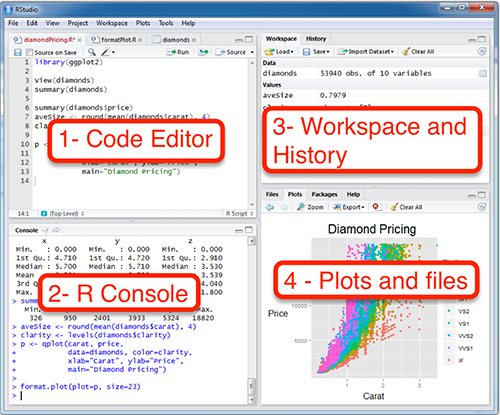
\includegraphics{images/010-intro_rstudio_tabs.png}

В первую очередь нас интересуют два окна: \textbf{1 - Code Editor} (окно
для написания скриптов)\footnote{При первом запуске RStudio вы не
  увидите это окно. Для того, чтобы оно появилось, нужно нажать
  \texttt{File\ -\ New\ File\ -\ R\ Script}.} и \textbf{2 - R Console}
(консоль). Здесь можно писать команды и запускать их. При этом работа в
консоли и работа со скриптом немного различается.

В \textbf{2 - R Console} вы пишите команду и запускаете ее нажиманием
\texttt{Enter}. Иногда после запуска команды появляется какой-то
результат. Если нажимать стрелку вверх на клавиатуре, то можно выводить
в консоль предыдущие команды. Это очень удобно для запуска предыдущих
команд с небольшими изменениями.

В \textbf{1 - Code Editor} для запуска команды вы должны выделить ее и
нажать \texttt{Ctrl} + \texttt{Enter} (\texttt{Cmd} + \texttt{Enter} на
macOS). Если не нажать эту комбинацию клавиш, то команда не запустится.
Можно выделить и запустить сразу несколько команд или даже все команды
скрипта. Все команды скрипта можно выделить с помощью сочетания клавиш
\texttt{Ctrl} + \texttt{A} на Windows и Linux, \texttt{Cmd} + \texttt{A}
на macOS \footnote{В RStudio есть много удобных сочетаний горячих
  клавиш. Чтобы посмотреть их все, нажмите
  \texttt{Help\ -\ Keyboard\ Shortcuts\ Help}.}. Как только вы запустите
команду (или несколько команд), соответствующие строчки кода появятся в
\textbf{2 - R Console}, как будто бы вы запускали их прямо там.

Обычно в консоли удобно что-то писать, чтобы быстро что-то посчитать.
Скрипты удобнее при работе с длинными командами и как способ сохранения
написанного кода для дальнейшей работы. Для сохранения скрипта нажмите
\texttt{File\ -\ Save\ As...}. R скрипты сохраняются с разрешением
\emph{.R}, но по своей сути это просто текстовые файлы, которые можно
открыть и модифицировать в любом текстовом редакторе а-ля ``Блокнот''.

\textbf{3 - Workspace and History} -- здесь можно увидеть переменные.
Это поле будет автоматически обновляться по мере того, как Вы будете
запускать строчки кода и создавать новые переменные. Еще там есть
вкладка с историей всех команд, которые были запущены.

\textbf{4 - Plots and files}. Здесь есть очень много всего. Во-первых,
небольшой файловый менеджер, во-вторых, там будут появляться графики,
когда вы будете их рисовать. Там же есть вкладка с вашими пакетами
(\texttt{Packages}) и \texttt{Help} по функциям. Но об этом потом.

\hypertarget{sec-calc}{%
\section{R как калькулятор}\label{sec-calc}}

R -- полноценный язык программирования, который позволяет решать широкий
спектр задач. Но в первую очередь R используется для анализа данных и
статистических вычислений. Тем не менее, многими R до сих пор
воспринимается как просто продвинутый калькулятор. Ну что ж,
калькулятор, так калькулятор.

Давайте начнем с самого простого и попробуем использовать R как
калькулятор с помощью арифметических операторов \texttt{+}, \texttt{-},
\texttt{*}, \texttt{/}, \texttt{\^{}} (степень), \texttt{()} и т.д.

Просто запускайте в консоли пока не надоест:

\begin{Shaded}
\begin{Highlighting}[]
\DecValTok{40}\SpecialCharTok{+}\DecValTok{2}
\end{Highlighting}
\end{Shaded}

\begin{verbatim}
[1] 42
\end{verbatim}

\begin{Shaded}
\begin{Highlighting}[]
\DecValTok{3{-}2}
\end{Highlighting}
\end{Shaded}

\begin{verbatim}
[1] 1
\end{verbatim}

\begin{Shaded}
\begin{Highlighting}[]
\DecValTok{5}\SpecialCharTok{*}\DecValTok{6}
\end{Highlighting}
\end{Shaded}

\begin{verbatim}
[1] 30
\end{verbatim}

\begin{Shaded}
\begin{Highlighting}[]
\DecValTok{99}\SpecialCharTok{/}\DecValTok{9} \CommentTok{\#деление}
\end{Highlighting}
\end{Shaded}

\begin{verbatim}
[1] 11
\end{verbatim}

\begin{Shaded}
\begin{Highlighting}[]
\DecValTok{2}\SpecialCharTok{\^{}}\DecValTok{3} \CommentTok{\#степень}
\end{Highlighting}
\end{Shaded}

\begin{verbatim}
[1] 8
\end{verbatim}

\begin{Shaded}
\begin{Highlighting}[]
\DecValTok{13} \SpecialCharTok{\%/\%} \DecValTok{3} \CommentTok{\#целочисленное деление}
\end{Highlighting}
\end{Shaded}

\begin{verbatim}
[1] 4
\end{verbatim}

\begin{Shaded}
\begin{Highlighting}[]
\DecValTok{13} \SpecialCharTok{\%\%} \DecValTok{3} \CommentTok{\#остаток от деления}
\end{Highlighting}
\end{Shaded}

\begin{verbatim}
[1] 1
\end{verbatim}

\begin{tcolorbox}[enhanced jigsaw, leftrule=.75mm, toprule=.15mm, left=2mm, breakable, arc=.35mm, rightrule=.15mm, colback=white, opacityback=0, bottomrule=.15mm]

\textbf{Время мемов}\vspace{2mm}

Попробуйте самостоятельно посчитать что-нибудь с разными числами.


\includegraphics[width=4.16667in,height=\textheight]{images/010-intro_meme_practical_cat.jpg}

\end{tcolorbox}

Ничего сложного, верно? Вводим выражение и получаем результат.

\begin{tcolorbox}[enhanced jigsaw, leftrule=.75mm, toprule=.15mm, left=2mm, breakable, arc=.35mm, rightrule=.15mm, colback=white, opacityback=0, bottomrule=.15mm]

\textbf{\emph{Полезное:} комментарии}\vspace{2mm}

Вы могли заметить, что некоторые команды у меня заканчиваются знаком
решетки (\texttt{\#}). Все, что написано в строчке после \texttt{\#}
игнорируется R при выполнении команды. Написанные команды в скрипте
рекомендуется сопровождать комментариями, которые будут объяснять вам же
в будущем (или кому-то еще), что конкретно происходит в соответствующем
куске кода \footnote{Во время написания кода вам может казаться понятным
  то, что вы написали, но при возвращении к коду через некоторое время
  вы уже не будете этого помнить. Старайтесь писать комментарии как
  можно чаще!}. Кроме того, комментарии можно использовать в тех
случаях, когда вы хотите написать кусок кода по-другому, не стирая
полностью предыдущий код: достаточно ``закомментить'' нужные строчки -
поставить \texttt{\#} в начало каждой строки, которую вы хотите
переписать. Для этого есть специальное сочетание горячих клавиш:
\texttt{Ctrl} + \texttt{Shift} + \texttt{C} (\texttt{Cmd} +
\texttt{Shift} + \texttt{C} на macOS) -- во всех выделенных строчках
будет написан \texttt{\#} в начале.

\end{tcolorbox}

Согласно данным навязчивых рекламных баннеров в интернете, только 14\%
россиян могут справиться с этим примером:

\begin{Shaded}
\begin{Highlighting}[]
\DecValTok{2} \SpecialCharTok{+} \DecValTok{2} \SpecialCharTok{*} \DecValTok{2}
\end{Highlighting}
\end{Shaded}

\begin{verbatim}
[1] 6
\end{verbatim}

На самом деле, разные языки программирования ведут себя
\href{https://www.quora.com/Do-all-computer-languages-with-operator-precedence-use-the-same-operator-precedence}{по-разному}
в таких ситуациях, поэтому ответ 6 (сначала умножаем, потом складываем)
не так очевиден.

Порядок выполнения арифметических операций (т.е. приоритет операторов,
\emph{operator precedence}) в R как в математике, так что не забывайте
про скобочки.

\begin{Shaded}
\begin{Highlighting}[]
\NormalTok{(}\DecValTok{2} \SpecialCharTok{+} \DecValTok{2}\NormalTok{) }\SpecialCharTok{*} \DecValTok{2}
\end{Highlighting}
\end{Shaded}

\begin{verbatim}
[1] 8
\end{verbatim}

Если Вы не уверены в том, какие операторы имеют приоритет, то
используйте скобочки, чтобы точно обозначить, в каком порядке нужно
производить операции. Или же смотрите на таблицу приоритета операторов с
помощью команды \texttt{?Syntax}.

\hypertarget{sec-func}{%
\section{Функции}\label{sec-func}}

Давайте теперь извлечем корень из какого-нибудь числа. В принципе, тем,
кто помнит школьный курс математики, возведения в степень вполне
достаточно:

\begin{Shaded}
\begin{Highlighting}[]
\DecValTok{16} \SpecialCharTok{\^{}} \FloatTok{0.5}
\end{Highlighting}
\end{Shaded}

\begin{verbatim}
[1] 4
\end{verbatim}

Ну а если нет, то можете воспользоваться специальной \textbf{функцией}:
это обычно какие-то буквенные символы с круглыми скобками сразу после
названия функции. Мы подаем на вход (внутрь скобочек) какие-то данные,
внутри этих функций происходят какие-то вычисления, которые выдает в
ответ какие-то другие данные (или же функция записывает файл, рисует
график и т.д.).

Вот, например, функция для корня:

\begin{Shaded}
\begin{Highlighting}[]
\FunctionTok{sqrt}\NormalTok{(}\DecValTok{16}\NormalTok{)}
\end{Highlighting}
\end{Shaded}

\begin{verbatim}
[1] 4
\end{verbatim}

\begin{tcolorbox}[enhanced jigsaw, leftrule=.75mm, toprule=.15mm, left=2mm, breakable, arc=.35mm, rightrule=.15mm, colback=white, opacityback=0, bottomrule=.15mm]

\textbf{Осторожно!}\vspace{2mm}

R -- case-sensitive язык, т.е. регистр важен. SQRT(16) не будет
работать.

\end{tcolorbox}

А вот так выглядит функция логарифма:

\begin{Shaded}
\begin{Highlighting}[]
\FunctionTok{log}\NormalTok{(}\DecValTok{8}\NormalTok{)}
\end{Highlighting}
\end{Shaded}

\begin{verbatim}
[1] 2.079442
\end{verbatim}

Так, вроде бы все нормально, но\ldots{} Если Вы еще что-то помните из
школьной математики, то должны понимать, что что-то здесь не так.

Здесь не хватает основания логарифма!

\begin{quote}
Логарифм -- показатель степени, в которую надо возвести число,
называемое основанием, чтобы получить данное число.
\end{quote}

То есть у логарифма 8 по основанию 2 будет значение 3:

\(\log_2 8 = 3\)

То есть если возвести 2 в степень 3 у нас будет 8:

\(2^3 = 8\)

Только наша функция считает все как-то не так.

Чтобы понять, что происходит, нам нужно залезть в хэлп этой функции:

\begin{Shaded}
\begin{Highlighting}[]
\NormalTok{?log}
\end{Highlighting}
\end{Shaded}

Справа внизу в RStudio появится вот такое окно:

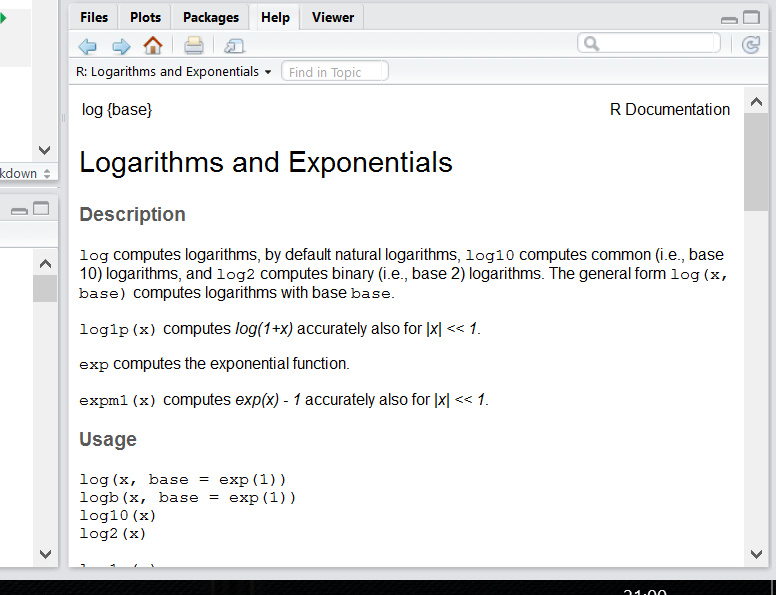
\includegraphics[width=4.16667in,height=\textheight]{images/010-intro_screen_use_help.png}

Действительно, у этой функции есть еще аргумент \emph{\texttt{base\ =}}.
По умолчанию он равен числу Эйлера (2.7182818\ldots), т.е. функция
считает натуральный логарифм. В большинстве функций R есть какой-то
основной инпут -- данные в том или ином формате, а есть и дополнительные
параметры, которые можно прописывать вручную, если параметры по
умолчанию вас не устраивают.

\begin{Shaded}
\begin{Highlighting}[]
\FunctionTok{log}\NormalTok{(}\AttributeTok{x =} \DecValTok{8}\NormalTok{, }\AttributeTok{base =} \DecValTok{2}\NormalTok{)}
\end{Highlighting}
\end{Shaded}

\begin{verbatim}
[1] 3
\end{verbatim}

\ldots или просто (если Вы уверены в порядке переменных):

\begin{Shaded}
\begin{Highlighting}[]
\FunctionTok{log}\NormalTok{(}\DecValTok{8}\NormalTok{, }\DecValTok{2}\NormalTok{)}
\end{Highlighting}
\end{Shaded}

\begin{verbatim}
[1] 3
\end{verbatim}

Более того, Вы можете использовать результат выполнения одних функций в
качестве аргумента для других:

\begin{Shaded}
\begin{Highlighting}[]
\FunctionTok{log}\NormalTok{(}\DecValTok{8}\NormalTok{, }\FunctionTok{sqrt}\NormalTok{(}\DecValTok{4}\NormalTok{))}
\end{Highlighting}
\end{Shaded}

\begin{verbatim}
[1] 3
\end{verbatim}

Если эксплицитно писать имена аргументов, то их порядок в функции не
важен:

\begin{Shaded}
\begin{Highlighting}[]
\FunctionTok{log}\NormalTok{(}\AttributeTok{base =} \DecValTok{2}\NormalTok{, }\AttributeTok{x =} \DecValTok{8}\NormalTok{)}
\end{Highlighting}
\end{Shaded}

\begin{verbatim}
[1] 3
\end{verbatim}

А еще можно писать имена аргументов не полностью, если они не совпадают
с другими:

\begin{Shaded}
\begin{Highlighting}[]
\FunctionTok{log}\NormalTok{(}\AttributeTok{b =} \DecValTok{2}\NormalTok{, }\AttributeTok{x =} \DecValTok{8}\NormalTok{)}
\end{Highlighting}
\end{Shaded}

\begin{verbatim}
[1] 3
\end{verbatim}

Мы еще много раз будем возвращаться к функциям. Вообще, функции -- это
одна из важнейших штук в R (примерно так же как и в \emph{Python}). Мы
будем создавать свои функции, использовать функции как аргументы для
функций и многое-многое другое. В R очень крутые возможности работы с
функциями. Поэтому подружитесь с функциями, они клевые.

\begin{tcolorbox}[enhanced jigsaw, leftrule=.75mm, toprule=.15mm, left=2mm, breakable, arc=.35mm, rightrule=.15mm, colback=white, opacityback=0, bottomrule=.15mm]

\textbf{\emph{Для продвинутых:} операторы -- это тоже
функции}\vspace{2mm}

Арифметические знаки, которые мы использовали:
\texttt{+},\texttt{-},\texttt{/},\texttt{\^{}} и т.д. называются
\textbf{операторами} и на самом деле тоже являются функциями:

\begin{Shaded}
\begin{Highlighting}[]
\StringTok{\textasciigrave{}}\AttributeTok{+}\StringTok{\textasciigrave{}}\NormalTok{(}\DecValTok{3}\NormalTok{, }\DecValTok{4}\NormalTok{)}
\end{Highlighting}
\end{Shaded}

\begin{verbatim}
[1] 7
\end{verbatim}

Это не очень читаемая запись, конечно, поэтому использовать так обычно
не рекомендуется: мы хотим, чтобы код был максимально понятным. Но ведь
любопытно, правда?

\end{tcolorbox}

\hypertarget{sec-google}{%
\section{В любой непонятной ситуации -- гуглите}\label{sec-google}}

Если вдруг вы не знаете, что искать в хэлпе, или хэлпа попросту
недостаточно, то\ldots{} гуглите!

\begin{tcolorbox}[enhanced jigsaw, leftrule=.75mm, toprule=.15mm, left=2mm, breakable, arc=.35mm, rightrule=.15mm, colback=white, opacityback=0, bottomrule=.15mm]

\textbf{Время мемов}\vspace{2mm}


\includegraphics{images/010-intro_meme_doctors_googling.jpg}

\end{tcolorbox}

Нет ничего постыдного в том, чтобы гуглить решения проблем. Это
абсолютно нормально. Используйте силу интернета во благо и да помогут
вам \href{https://stackoverflow.com}{\emph{Stackoverflow}}\footnote{\href{https://stackoverflow.com}{Stackoverflow}
  -- это сайт с вопросами и ответами. Эдакий аналог \emph{Quora},
  \emph{The Question}, ну или \emph{Ответы Mail.ru} в мире
  программирования.} и бесчисленные R-туториалы!

\begin{tcolorbox}[enhanced jigsaw, leftrule=.75mm, toprule=.15mm, left=2mm, breakable, arc=.35mm, rightrule=.15mm, colback=white, opacityback=0, bottomrule=.15mm]

\textbf{Время мемов}\vspace{2mm}


\includegraphics{images/010_intro_copypaste_stack.png}

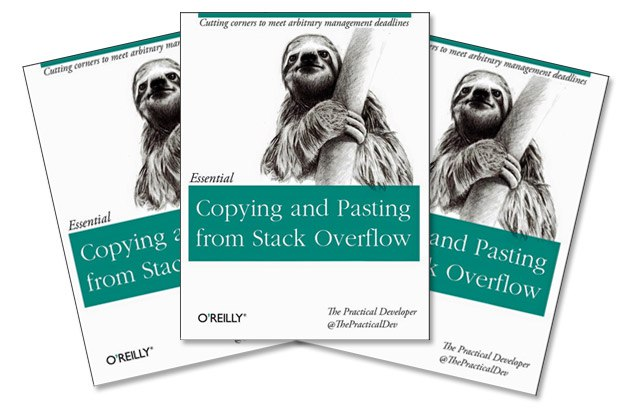
\includegraphics{images/010-intro_meme_copypaste_lazy.jpg}

\end{tcolorbox}

Главное, помните: загуглить работающий ответ всегда недостаточно. Надо
понять, как и почему решение работает. Иначе что-то обязательно пойдет
не так.

Кроме того, правильно загуглить проблему -- не так уж и просто. Это
отдельное искусство, которое необходимо освоить любому, кто занимается
программированием: у меня быстро находить ответ на вопрос в интернете.
Это не шутка!

\begin{tcolorbox}[enhanced jigsaw, leftrule=.75mm, toprule=.15mm, left=2mm, breakable, arc=.35mm, rightrule=.15mm, colback=white, opacityback=0, bottomrule=.15mm]

\textbf{Время мемов}\vspace{2mm}


\includegraphics[width=6.25in,height=\textheight]{images/010_intro_goot_at_googling_twitter.png}

\end{tcolorbox}

Короче говоря:

\begin{quote}
Гуглить -- хорошо, бездумно копировать чужие решения -- плохо.
\end{quote}

\hypertarget{sec-variables}{%
\section{Переменные}\label{sec-variables}}

Важная штука в программировании на практически любом языке --
возможность сохранять значения в \textbf{переменных \emph{(variables)}}.
В R это обычно делается с помощью вот этих символов:
\texttt{\textless{}-} (но можно использовать и обычное \texttt{=}, хотя
это не очень принято). Для этого есть удобное сочетание клавиш: нажмите
одновременно \texttt{Alt} + \texttt{-} (или \texttt{option} + \texttt{-}
в macOS).

\begin{Shaded}
\begin{Highlighting}[]
\NormalTok{a }\OtherTok{\textless{}{-}} \DecValTok{2}
\end{Highlighting}
\end{Shaded}

\begin{tcolorbox}[enhanced jigsaw, leftrule=.75mm, toprule=.15mm, left=2mm, breakable, arc=.35mm, rightrule=.15mm, colback=white, opacityback=0, bottomrule=.15mm]

\textbf{Полезное: присвоение и вывод в консоль}\vspace{2mm}

Заметьте, при присвоении результат вычисления не выводится в консоль!
Если опустить детали, то обычно результат выполнения команды либо
выводится в консоль (и не сохраняется), либо записывается в переменную
(но тогда не показывается в консоли).

Чтобы вывести в консоль содержание существующей переменной, просто
введите ее название:

\begin{Shaded}
\begin{Highlighting}[]
\NormalTok{a}
\end{Highlighting}
\end{Shaded}

\begin{verbatim}
[1] 2
\end{verbatim}

\end{tcolorbox}

Справа от \texttt{\textless{}-} находится значение, которое вы хотите
сохранить, или же какое-то выражение, результат которого вы хотите
сохранить в эту переменную\footnote{Есть еще оператор
  \texttt{-\textgreater{}}, который позволяет присваивать значения слева
  направо, но так делать не рекомендуется, хотя это бывает довольно
  удобным.}:

Слева от \texttt{\textless{}-} находится название будущей переменной.
Название переменных может быть самым разным.

\begin{tcolorbox}[enhanced jigsaw, leftrule=.75mm, toprule=.15mm, left=2mm, breakable, arc=.35mm, rightrule=.15mm, colback=white, opacityback=0, bottomrule=.15mm]

\textbf{\emph{Advanced:} синтаксически валидные имена для
переменных}\vspace{2mm}

Есть несколько ограничений для синтаксически валидных имен переменных:
они должны включать в себя буквы, цифры, \texttt{.} или \texttt{\_},
начинаться на букву (или точку, за которой не будет следовать цифра), не
должны совпадать с
\href{https://stat.ethz.ch/R-manual/R-devel/library/base/html/Reserved.html}{коротким
списком зарезервированных слов}. Короче говоря, название не должно
включать в себя пробелы и большинство других знаков.

Нельзя: - \texttt{new\ variable} - \texttt{\_new\_variable} -
\texttt{.1var} - \texttt{v-r}

Можно: - \texttt{new\_variable} - \texttt{.new.variable} -
\texttt{var\_2}

На самом деле, можно создавать переменные с невалидными именами. Такие
названия нужно обрамлять бэктиками (`):

\begin{Shaded}
\begin{Highlighting}[]
\StringTok{\textasciigrave{}}\AttributeTok{1 СЛОВНО ...}\StringTok{\textasciigrave{}} \OtherTok{\textless{}{-}} \DecValTok{100}
\StringTok{\textasciigrave{}}\AttributeTok{1 СЛОВНО ...}\StringTok{\textasciigrave{}}
\end{Highlighting}
\end{Shaded}

\begin{verbatim}
[1] 100
\end{verbatim}

Это же относится и к другим именам в R, например, к названиям колонок
датафрейма (см. Глава~\ref{sec-df}), но таких имен лучше, конечно,
избегать.

\end{tcolorbox}

\begin{tcolorbox}[enhanced jigsaw, leftrule=.75mm, toprule=.15mm, left=2mm, breakable, arc=.35mm, rightrule=.15mm, colback=white, opacityback=0, bottomrule=.15mm]

\textbf{\emph{Полезное:} понятные имена переменных}\vspace{2mm}

Обязательно делайте названия переменных осмысленными! Старайтесь делать
при этом их понятными и короткими, это сохранит вам очень много времени,
когда вы (или кто-то еще) будете пытаться разобраться в написанном ранее
коде. Если название все-таки получается длинным и состоящим из
нескольких слов, то лучше всего использовать нижнее подчеркивание в
качестве разделителя: \texttt{some\_variable}\footnote{Еще иногда
  используются большие буквы \texttt{SomeVariable}, но это плохо
  читается, а иногда -- точка, но это тоже не рекомендуется.}.

\end{tcolorbox}

После присвоения переменная появляется во вкладке \textbf{Environment} в
RStudio:

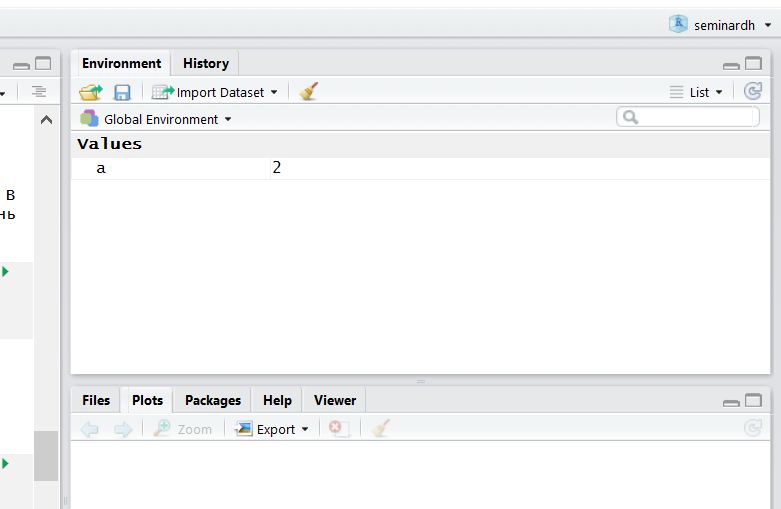
\includegraphics[width=4.16667in,height=\textheight]{images/env.png}

Теперь использовать переменные в функциях и просто вычислениях:

\begin{Shaded}
\begin{Highlighting}[]
\NormalTok{b }\OtherTok{\textless{}{-}}\NormalTok{ a }\SpecialCharTok{\^{}}\NormalTok{ a }\SpecialCharTok{+}\NormalTok{ a }\SpecialCharTok{*}\NormalTok{ a}
\NormalTok{b}
\end{Highlighting}
\end{Shaded}

\begin{verbatim}
[1] 8
\end{verbatim}

\begin{Shaded}
\begin{Highlighting}[]
\FunctionTok{log}\NormalTok{(b, a)}
\end{Highlighting}
\end{Shaded}

\begin{verbatim}
[1] 3
\end{verbatim}

Удалять переменные можно с помощью функции \texttt{rm()}:

\begin{Shaded}
\begin{Highlighting}[]
\NormalTok{e }\OtherTok{\textless{}{-}}\NormalTok{ a }\SpecialCharTok{\^{}}\NormalTok{ b}
\NormalTok{e}
\end{Highlighting}
\end{Shaded}

\begin{verbatim}
[1] 256
\end{verbatim}

\begin{Shaded}
\begin{Highlighting}[]
\FunctionTok{rm}\NormalTok{(e)}
\NormalTok{e }\CommentTok{\#переменной больше нет, возвращает ошибку}
\end{Highlighting}
\end{Shaded}

\begin{verbatim}
Error in eval(expr, envir, enclos): object 'e' not found
\end{verbatim}

\hypertarget{sec-logic}{%
\section{Логические операторы}\label{sec-logic}}

Вы можете сравнивать разные переменные:

\begin{Shaded}
\begin{Highlighting}[]
\NormalTok{a }\SpecialCharTok{==}\NormalTok{ b}
\end{Highlighting}
\end{Shaded}

\begin{verbatim}
[1] FALSE
\end{verbatim}

Заметьте, что сравнивая две переменные мы используем два знака равно
\texttt{==}, а не один \texttt{=}. Иначе это будет означать присвоение.

\begin{Shaded}
\begin{Highlighting}[]
\NormalTok{a }\OtherTok{=}\NormalTok{ b}
\NormalTok{a}
\end{Highlighting}
\end{Shaded}

\begin{verbatim}
[1] 8
\end{verbatim}

\begin{tcolorbox}[enhanced jigsaw, leftrule=.75mm, toprule=.15mm, left=2mm, breakable, arc=.35mm, rightrule=.15mm, colback=white, opacityback=0, bottomrule=.15mm]

\textbf{Время мемов}\vspace{2mm}

Теперь Вы сможете понять комикс про восстание роботов на следующей
странице (пусть он и совсем про другой язык программирования)

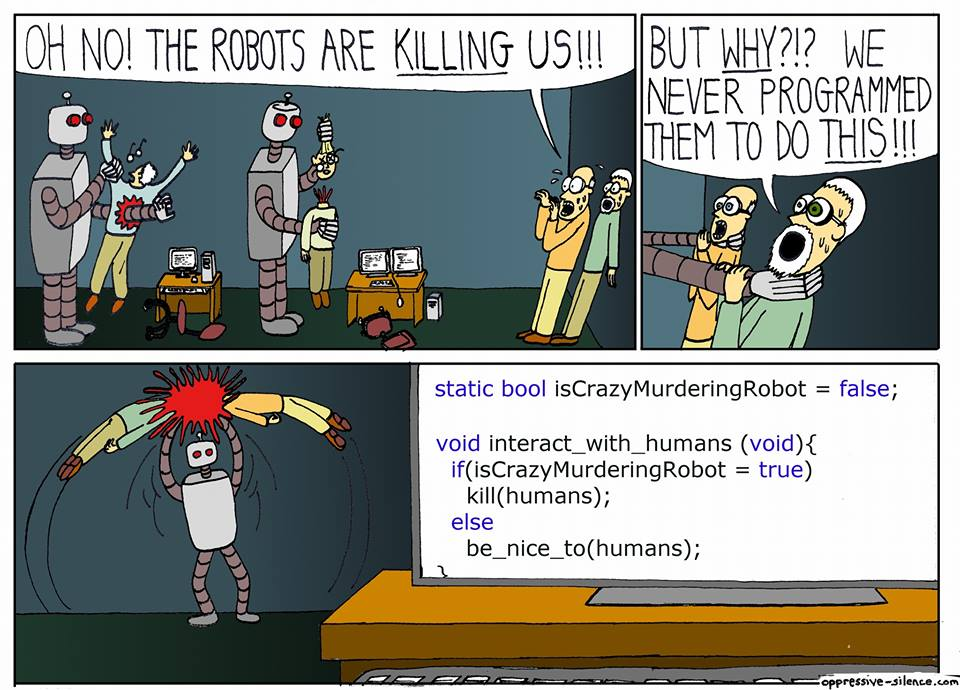
\includegraphics[width=4.16667in,height=\textheight]{images/WaCM5x3mvQM.jpg}

Этот комикс объясняет, как важно не путать присваивание и сравнение
\emph{(хотя я иногда путаю до сих пор =( )}.

\end{tcolorbox}

Иногда нам нужно проверить на \textbf{\emph{не}}равенство:

\begin{Shaded}
\begin{Highlighting}[]
\NormalTok{a }\OtherTok{\textless{}{-}} \DecValTok{2}
\NormalTok{b }\OtherTok{\textless{}{-}} \DecValTok{3}

\NormalTok{a }\SpecialCharTok{==}\NormalTok{ b}
\end{Highlighting}
\end{Shaded}

\begin{verbatim}
[1] FALSE
\end{verbatim}

\begin{Shaded}
\begin{Highlighting}[]
\NormalTok{a }\SpecialCharTok{!=}\NormalTok{ b}
\end{Highlighting}
\end{Shaded}

\begin{verbatim}
[1] TRUE
\end{verbatim}

Восклицательный язык в программировании вообще и в R в частности
стандартно означает отрицание.

Еще мы можем сравнивать на больше/меньше:

\begin{Shaded}
\begin{Highlighting}[]
\NormalTok{a }\SpecialCharTok{\textgreater{}}\NormalTok{ b}
\end{Highlighting}
\end{Shaded}

\begin{verbatim}
[1] FALSE
\end{verbatim}

\begin{Shaded}
\begin{Highlighting}[]
\NormalTok{a }\SpecialCharTok{\textless{}}\NormalTok{ b}
\end{Highlighting}
\end{Shaded}

\begin{verbatim}
[1] TRUE
\end{verbatim}

\begin{Shaded}
\begin{Highlighting}[]
\NormalTok{a }\SpecialCharTok{\textgreater{}=}\NormalTok{ b}
\end{Highlighting}
\end{Shaded}

\begin{verbatim}
[1] FALSE
\end{verbatim}

\begin{Shaded}
\begin{Highlighting}[]
\NormalTok{a }\SpecialCharTok{\textless{}=}\NormalTok{ b}
\end{Highlighting}
\end{Shaded}

\begin{verbatim}
[1] TRUE
\end{verbatim}

Этим мы будем пользоваться в дальнейшем регулярно! Именно на таких
простых логических операциях построено большинство операций с данными.

\hypertarget{sec-data_types}{%
\section{Типы данных}\label{sec-data_types}}

\hypertarget{sec-type_numeric}{%
\subsection{Числовые типы}\label{sec-type_numeric}}

До этого момента мы работали только с \textbf{\emph{числами (numeric).}}
На самом деле, в R три типа \textbf{\emph{numeric:}}
\textbf{\emph{integer}} \textbf{(целые), \emph{double} (дробные),
\emph{complex} (комплексные числа)}\footnote{\textbf{Комплексные числа в
  R пишутся так: \texttt{complexnumber\ \textless{}-\ 2+2i}. \texttt{i}
  здесь - это та самая мнимая единица, которая является квадратным
  корнем из -1.}}. R сам будет конвертировать числа в нужный числовой
тип при необходимости, поэтому этим можно не заморачиваться за
исключением редких случаев.

Если же все-таки нужно задать конкретный тип числа эксплицитно, то можно
воспользоваться функциями \texttt{as.integer()}, \texttt{as.double()} и
\texttt{as.complex()}.

\begin{tcolorbox}[enhanced jigsaw, leftrule=.75mm, toprule=.15mm, left=2mm, breakable, arc=.35mm, rightrule=.15mm, colback=white, opacityback=0, bottomrule=.15mm]

\textbf{\emph{Для продвинутых:} числа не то, чем кажутся}\vspace{2mm}

Если число выглядит как целое, еще не факт, что это integer. Внутри оно
может храниться как дробное, но, как я уже написал, это обычно не так
важно. Но если очень нужно сделать именно integer, при создании числа
можно поставить в конце \texttt{L}:

\begin{Shaded}
\begin{Highlighting}[]
\FunctionTok{is.integer}\NormalTok{(}\DecValTok{5}\NormalTok{)}
\end{Highlighting}
\end{Shaded}

\begin{verbatim}
[1] FALSE
\end{verbatim}

\begin{Shaded}
\begin{Highlighting}[]
\FunctionTok{is.integer}\NormalTok{(5L)}
\end{Highlighting}
\end{Shaded}

\begin{verbatim}
[1] TRUE
\end{verbatim}

\end{tcolorbox}

\begin{tcolorbox}[enhanced jigsaw, leftrule=.75mm, toprule=.15mm, left=2mm, breakable, arc=.35mm, rightrule=.15mm, colback=white, opacityback=0, bottomrule=.15mm]

\textbf{\emph{Для продвинутых:} ограничения дробных чисел}\vspace{2mm}

Про \emph{double} есть еще один маленький секрет. Дело в том, что
дробные числа хранятся в R как
\href{https://ru.wikipedia.org/wiki/Число_двойной_точности}{числа с
плавающей запятой двойной точности} (отсюда и название --
\textbf{\emph{``double''},} т.е. \textbf{\emph{``double precision''}).}
Да-да, компьютеры неточные! Дробные числа в компьютере могут быть
записаны только с определенной степенью точности, поэтому иногда
встречаются вот такие вот ситуации:

\begin{Shaded}
\begin{Highlighting}[]
\FunctionTok{sqrt}\NormalTok{(}\DecValTok{2}\NormalTok{) }\SpecialCharTok{\^{}} \DecValTok{2} \SpecialCharTok{==} \DecValTok{2}
\end{Highlighting}
\end{Shaded}

\begin{verbatim}
[1] FALSE
\end{verbatim}

Казалось бы, с обоих сторон -- 2, почему же тогда \texttt{FALSE}? Дело в
том, что в обоих случаях это дробное число, которое не может равняться
ровно двум. Внутри это не два, а что-то вроде 2.0000\ldots.001 или
1.9999\ldots999, число записано как степени двойки и отображено в
десятичной системе. R не показывает все доступные цифры дробной части
ради удобства, поэтому показывает округление, и мы видим просто число 2.

Поэтому при сравнении двух чисел происходит не сравнение их разницы с
чистым круглым нулем, а сопоставление с очень маленьким числом --
\textbf{машинной ошибкой} или \textbf{машинным эпсилоном}
\textbf{\emph{(machine epsilon).}} Если разница между двумя дробными
числами меньше этого эпсилона, то числа считаются равными. Если выходят
за пределы этой ошибки, то нет. Размер машинного эпсилона можно
посмотреть с помощью \texttt{.Machine\$double.eps}.

Обычно это все работает хорошо, но некоторые операции ``выпрыгивают'' за
рамки этой ошибки, отсюда и такое ``странное'' поведение, которое иногда
может возникать при сравнении двух чисел. Если хотите углубиться в этот
вопрос, то можете почитать
\href{https://stackoverflow.com/questions/9508518/why-are-these-numbers-not-equal?noredirect=1\&lq=1}{здесь}.

Это довольно стандартная ситуация, характерная не только для R. Чтобы ее
избежать, можно воспользоваться функцией \texttt{all.equal()}:

\begin{Shaded}
\begin{Highlighting}[]
\FunctionTok{all.equal}\NormalTok{(}\FunctionTok{sqrt}\NormalTok{(}\DecValTok{2}\NormalTok{) }\SpecialCharTok{\^{}} \DecValTok{2}\NormalTok{, }\DecValTok{2}\NormalTok{)}
\end{Highlighting}
\end{Shaded}

\begin{verbatim}
[1] TRUE
\end{verbatim}

Еще один пример необычного поведения дробных чисел, связанный с их
``неточностью'', можно наблюдать в ситуациях, где вы ожидаете ноль, а
получаете что-то такое:

\begin{Shaded}
\begin{Highlighting}[]
\FunctionTok{sin}\NormalTok{(pi)}
\end{Highlighting}
\end{Shaded}

\begin{verbatim}
[1] 1.224647e-16
\end{verbatim}

По правилам тригонометрии, \(sin(\pi) = 0\), тогда откуда у нас это
странное число с \texttt{e-16} в конце?

Это то, что называется \emph{экспоненциальной записью (scientific
notation)} числа, которую R использует автоматически, если нужно
напечатать очень маленькое или очень большое число. Экспоненциальная
запись часто используется как в компьютерах, так и во многих науках, так
что читать ее полезно уметь.

Если перед нами очень маленькое число, то вместо того, чтобы писать
многочисленные нули, можно записать его как \(m\times 10^{n}\) , где
\(m\) -- число от 1 до 10, а \(n\) -- это отрицательная степень десяти:
\(10^{-1} = 0.1\), \(10^{-2} = 0.01\), \(10^{-3} = 0.001\), \ldots{} ,
\(10^{-16} = 0.0000000000000001\).

\texttt{е-16} в конце числа -- это и есть \$10\^{}\{-16\}\$, а
\texttt{1.224647} -- это множитель \(m\), на который полученное число с
очень большим количеством нулей умножается (точнее, только его первые
несколько цифр). Получается, что этот множитель не сильно меняет погоды,
поэтому когда видите число с \texttt{е-}, нужно смотреть в первую
очередь именно на степень. Вот так это число выглядит в родной для нас
десятичной записи:

\begin{Shaded}
\begin{Highlighting}[]
\FunctionTok{format}\NormalTok{(}\FunctionTok{sin}\NormalTok{(pi), }\AttributeTok{scientific =} \ConstantTok{FALSE}\NormalTok{)}
\end{Highlighting}
\end{Shaded}

\begin{verbatim}
[1] "0.0000000000000001224647"
\end{verbatim}

Эта маленькая дробная часть возникла из-за этой ``неточности'' хранения
дробных чисел и самого числа \(\pi\) в компьютере, которую мы обсуждали
выше.

Аналогично маленьким числам, R использует экспоненциальную запись, когда
нужно напечатать очень большое число:

\begin{Shaded}
\begin{Highlighting}[]
\DecValTok{2} \SpecialCharTok{\^{}} \DecValTok{40}
\end{Highlighting}
\end{Shaded}

\begin{verbatim}
[1] 1.099512e+12
\end{verbatim}

Обратите внимание, что здесь у нас \texttt{e+12}, а не \texttt{e-12},
что означает \$10\^{}\{12\}\$, а не \$10\^{}\{-12\}\$. То есть перед
нами теперь \(1.099512\times 10^{12}\):

\begin{Shaded}
\begin{Highlighting}[]
\FunctionTok{format}\NormalTok{(}\DecValTok{2} \SpecialCharTok{\^{}} \DecValTok{40}\NormalTok{, }\AttributeTok{scientific =} \ConstantTok{FALSE}\NormalTok{)}
\end{Highlighting}
\end{Shaded}

\begin{verbatim}
[1] "1099511627776"
\end{verbatim}

Опять же, \texttt{1.099512} -- это только первые цифры, в
экспоненциальной записи R не показывает их все. Смотреть нужно сначала
на степень (\texttt{e+12}), только потом -- на множитель впереди.

\end{tcolorbox}

\hypertarget{sec-type_character}{%
\subsection{Строковый тип}\label{sec-type_character}}

\textbf{Строковые \emph{(character)}} данные -- это набор букв, цифр и
символов. Чтобы создать строковую переменную, нужные знаки обособляются
кавычками.

\begin{Shaded}
\begin{Highlighting}[]
\NormalTok{s }\OtherTok{\textless{}{-}} \StringTok{"Всем привет!"}
\NormalTok{s}
\end{Highlighting}
\end{Shaded}

\begin{verbatim}
[1] "Всем привет!"
\end{verbatim}

\begin{Shaded}
\begin{Highlighting}[]
\FunctionTok{class}\NormalTok{(s)}
\end{Highlighting}
\end{Shaded}

\begin{verbatim}
[1] "character"
\end{verbatim}

Как и в \emph{Python}, можно использовать как \texttt{"}, так и
\texttt{\textquotesingle{}} (что удобно, когда строчка внутри уже
содержит какие-то кавычки).

\begin{Shaded}
\begin{Highlighting}[]
\StringTok{"Ph\textquotesingle{}nglui mglw\textquotesingle{}nafh Cthulhu R\textquotesingle{}lyeh wgah\textquotesingle{}nagl fhtagn"}
\end{Highlighting}
\end{Shaded}

\begin{verbatim}
[1] "Ph'nglui mglw'nafh Cthulhu R'lyeh wgah'nagl fhtagn"
\end{verbatim}

Главное, открывать и закрывать кавычки одинаковыми кавычками (
\texttt{"} или \texttt{\textquotesingle{}})

Чтобы соединить несколько строковых переменных вместе, можно
воспользоваться функцией \texttt{paste()}\footnote{Оператор \texttt{+},
  в отличие от Python, не работает для соединения строк.}:

\begin{Shaded}
\begin{Highlighting}[]
\FunctionTok{paste}\NormalTok{(}\StringTok{"I"}\NormalTok{, }\StringTok{"love"}\NormalTok{, }\StringTok{"R"}\NormalTok{)}
\end{Highlighting}
\end{Shaded}

\begin{verbatim}
[1] "I love R"
\end{verbatim}

По умолчанию функция \texttt{paste()} соединяет строки пробелами, но
разделитель можно настроить параметром \texttt{sep\ =}:

\begin{Shaded}
\begin{Highlighting}[]
\FunctionTok{paste}\NormalTok{(}\StringTok{"I"}\NormalTok{, }\StringTok{"love"}\NormalTok{, }\StringTok{"R"}\NormalTok{, }\AttributeTok{sep =} \StringTok{"\_\textless{}3\_"}\NormalTok{)}
\end{Highlighting}
\end{Shaded}

\begin{verbatim}
[1] "I_<3_love_<3_R"
\end{verbatim}

Чтобы соединять строки, так сказать, ``без ничего'', нужно поставить
\texttt{sep\ =\ ""} или же воспользоваться функцией \texttt{paste0()}
специально для этого конкретного случая:

\begin{Shaded}
\begin{Highlighting}[]
\FunctionTok{paste}\NormalTok{(}\StringTok{"I"}\NormalTok{, }\StringTok{"love"}\NormalTok{, }\StringTok{"R"}\NormalTok{, }\AttributeTok{sep =} \StringTok{""}\NormalTok{)}
\end{Highlighting}
\end{Shaded}

\begin{verbatim}
[1] "IloveR"
\end{verbatim}

\begin{Shaded}
\begin{Highlighting}[]
\FunctionTok{paste0}\NormalTok{(}\StringTok{"I"}\NormalTok{, }\StringTok{"love"}\NormalTok{, }\StringTok{"R"}\NormalTok{)}
\end{Highlighting}
\end{Shaded}

\begin{verbatim}
[1] "IloveR"
\end{verbatim}

\hypertarget{sec-type_logical}{%
\subsection{Логический тип}\label{sec-type_logical}}

\textbf{Логические (logical)} данные -- это просто \texttt{TRUE} или
\texttt{FALSE}.

\begin{Shaded}
\begin{Highlighting}[]
\NormalTok{t1 }\OtherTok{\textless{}{-}} \ConstantTok{TRUE}
\NormalTok{f1 }\OtherTok{\textless{}{-}} \ConstantTok{FALSE}

\NormalTok{t1}
\end{Highlighting}
\end{Shaded}

\begin{verbatim}
[1] TRUE
\end{verbatim}

\begin{Shaded}
\begin{Highlighting}[]
\NormalTok{f1}
\end{Highlighting}
\end{Shaded}

\begin{verbatim}
[1] FALSE
\end{verbatim}

\begin{tcolorbox}[enhanced jigsaw, leftrule=.75mm, toprule=.15mm, left=2mm, breakable, arc=.35mm, rightrule=.15mm, colback=white, opacityback=0, bottomrule=.15mm]

\textbf{\emph{Для продвинутых:} \texttt{T} и \texttt{F}}\vspace{2mm}

Вообще, можно еще писать \texttt{T} и \texttt{F} (но не \texttt{True} и
\texttt{False}!)

\begin{Shaded}
\begin{Highlighting}[]
\NormalTok{t1 }\OtherTok{\textless{}{-}}\NormalTok{ T}
\NormalTok{f1 }\OtherTok{\textless{}{-}}\NormalTok{ F}
\end{Highlighting}
\end{Shaded}

Это плохая практика: R защищает от перезаписи переменные \texttt{TRUE} и
\texttt{FALSE}, но не защищает от этого \texttt{T} и \texttt{F}.

\begin{Shaded}
\begin{Highlighting}[]
\ConstantTok{TRUE} \OtherTok{\textless{}{-}} \ConstantTok{FALSE}
\end{Highlighting}
\end{Shaded}

\begin{verbatim}
Error in TRUE <- FALSE: invalid (do_set) left-hand side to assignment
\end{verbatim}

\begin{Shaded}
\begin{Highlighting}[]
\ConstantTok{TRUE}
\end{Highlighting}
\end{Shaded}

\begin{verbatim}
[1] TRUE
\end{verbatim}

\begin{Shaded}
\begin{Highlighting}[]
\NormalTok{T }\OtherTok{\textless{}{-}} \ConstantTok{FALSE}
\NormalTok{T}
\end{Highlighting}
\end{Shaded}

\begin{verbatim}
[1] FALSE
\end{verbatim}

Теперь удалим эту переменную \texttt{T} от греха подальше:

\begin{Shaded}
\begin{Highlighting}[]
\FunctionTok{rm}\NormalTok{(T)}
\end{Highlighting}
\end{Shaded}

\end{tcolorbox}

Мы уже встречались с логическими значениями при сравнении двух числовых
переменных. Теперь вы можете догадаться, что результаты сравнения,
например, числовых или строковых переменных, можно тоже сохранять в
переменные!

\begin{Shaded}
\begin{Highlighting}[]
\NormalTok{comparison }\OtherTok{\textless{}{-}}\NormalTok{ a }\SpecialCharTok{==}\NormalTok{ b}
\NormalTok{comparison}
\end{Highlighting}
\end{Shaded}

\begin{verbatim}
[1] FALSE
\end{verbatim}

Это нам очень понадобится, когда мы будем работать с реальными данными:
нам нужно будет постоянно вытаскивать какие-то данные из датасета, что
как раз и построено на игре со сравнением переменных.

Чтобы этим хорошо уметь пользоваться, нам нужно еще освоить как работать
с логическими операторами. Про один мы немного уже говорили -- это
логическое НЕ (\texttt{!}). \texttt{!} превращает \texttt{TRUE} в
\texttt{FALSE}, а \texttt{FALSE} в \texttt{TRUE}:

\begin{Shaded}
\begin{Highlighting}[]
\NormalTok{t1}
\end{Highlighting}
\end{Shaded}

\begin{verbatim}
[1] TRUE
\end{verbatim}

\begin{Shaded}
\begin{Highlighting}[]
\SpecialCharTok{!}\NormalTok{t1}
\end{Highlighting}
\end{Shaded}

\begin{verbatim}
[1] FALSE
\end{verbatim}

\begin{Shaded}
\begin{Highlighting}[]
\SpecialCharTok{!!}\NormalTok{t1 }\CommentTok{\#Двойное отрицание!}
\end{Highlighting}
\end{Shaded}

\begin{verbatim}
[1] TRUE
\end{verbatim}

Еще есть логическое И (выдаст \texttt{TRUE} только в том случае если обе
переменные \texttt{TRUE}):

\begin{Shaded}
\begin{Highlighting}[]
\NormalTok{t1 }\SpecialCharTok{\&}\NormalTok{ t1}
\end{Highlighting}
\end{Shaded}

\begin{verbatim}
[1] TRUE
\end{verbatim}

\begin{Shaded}
\begin{Highlighting}[]
\NormalTok{t1 }\SpecialCharTok{\&}\NormalTok{ f1}
\end{Highlighting}
\end{Shaded}

\begin{verbatim}
[1] FALSE
\end{verbatim}

\begin{Shaded}
\begin{Highlighting}[]
\NormalTok{f1 }\SpecialCharTok{\&}\NormalTok{ t1}
\end{Highlighting}
\end{Shaded}

\begin{verbatim}
[1] FALSE
\end{verbatim}

\begin{Shaded}
\begin{Highlighting}[]
\NormalTok{f1 }\SpecialCharTok{\&}\NormalTok{ f1}
\end{Highlighting}
\end{Shaded}

\begin{verbatim}
[1] FALSE
\end{verbatim}

А еще логическое ИЛИ (выдаст \texttt{TRUE} в случае если хотя бы одна из
переменных \texttt{TRUE}):

\begin{Shaded}
\begin{Highlighting}[]
\NormalTok{t1 }\SpecialCharTok{|}\NormalTok{ t1}
\end{Highlighting}
\end{Shaded}

\begin{verbatim}
[1] TRUE
\end{verbatim}

\begin{Shaded}
\begin{Highlighting}[]
\NormalTok{t1 }\SpecialCharTok{|}\NormalTok{ f1}
\end{Highlighting}
\end{Shaded}

\begin{verbatim}
[1] TRUE
\end{verbatim}

\begin{Shaded}
\begin{Highlighting}[]
\NormalTok{f1 }\SpecialCharTok{|}\NormalTok{ t1}
\end{Highlighting}
\end{Shaded}

\begin{verbatim}
[1] TRUE
\end{verbatim}

\begin{Shaded}
\begin{Highlighting}[]
\NormalTok{f1 }\SpecialCharTok{|}\NormalTok{ f1}
\end{Highlighting}
\end{Shaded}

\begin{verbatim}
[1] FALSE
\end{verbatim}

Обратите внимание: \texttt{t1\ \textbar{}\ t1}, то есть когда с обоих
сторон \texttt{TRUE}, тоже возвращает \texttt{TRUE}!

\begin{tcolorbox}[enhanced jigsaw, leftrule=.75mm, toprule=.15mm, left=2mm, breakable, arc=.35mm, rightrule=.15mm, colback=white, opacityback=0, bottomrule=.15mm]

\textbf{\emph{Для продвинутых:} строгое ЛИБО}\vspace{2mm}

Если кому-то вдруг понадобится другое ИЛИ (строгое ЛИБО) -- есть функция
\texttt{xor()}, принимающая два аргумента и возвращая \texttt{TRUE}
только в том случае, если ровно один из двух аргументов равен
\texttt{TRUE}. Но на практике она нужна очень редко, тогда как
логические И и ИЛИ нужны очень часто: например, вам нужно отобрать
только респондентов от 18 до 25, для этого нужно сделать два сравнения:
что возраст больше 18 и что возраст меньше 25, после чего соединить два
сравнения логическим И.

\end{tcolorbox}

Итак, мы только что разобрались с самой занудной (хотя и важной) частью
- с основными типа данных в R и как с ними работать\footnote{Кроме
  описанных пяти типов данных (integer, double, complex, character и
  logical) есть еще и шестой -- это raw, сырая последовательность
  байтов, но нам она не понадобится.}. Пора переходить к чему-то более
интересному и специфическому для R. Вперед к ВЕКТОРАМ!

\hypertarget{sec-vector}{%
\chapter{Вектор}\label{sec-vector}}

\hypertarget{sec-atomic}{%
\section{Понятие atomic вектора в R}\label{sec-atomic}}

Если у вас не было линейной алгебры (или у вас с ней было все плохо), то
просто запомните, что \textbf{вектор} (\textbf{\emph{atomic vector}} или
просто \textbf{\emph{atomic}}) -- это набор (столбик) чисел в
определенном порядке.

Если вы привыкли из школьного курса физики считать вектора стрелочками,
то не спешите возмущаться и паниковать. Представьте стрелочки как точки
из нуля координат \{0,0\} до какой-то точки на координатной плоскости,
например, \{2,3\}:

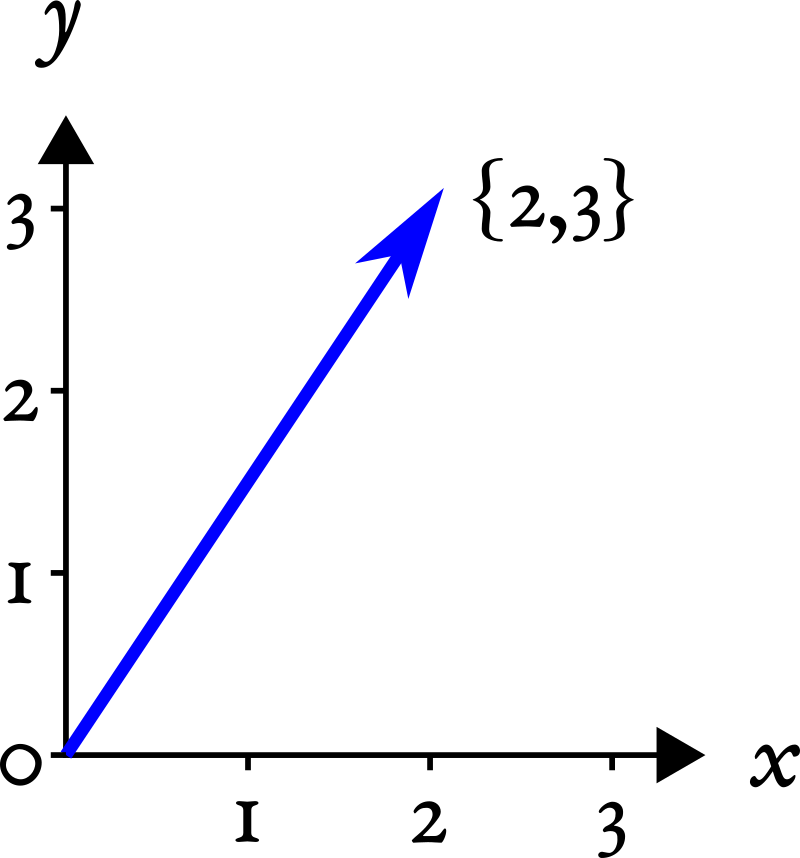
\includegraphics[width=4.16667in,height=\textheight]{images/coord_vector.png}

Вот последние два числа и будем считать вектором. Попытайтесь теперь
мысленно стереть координатную плоскость и выбросить стрелочки из головы,
оставив только последовательность чисел \{2,3\}:

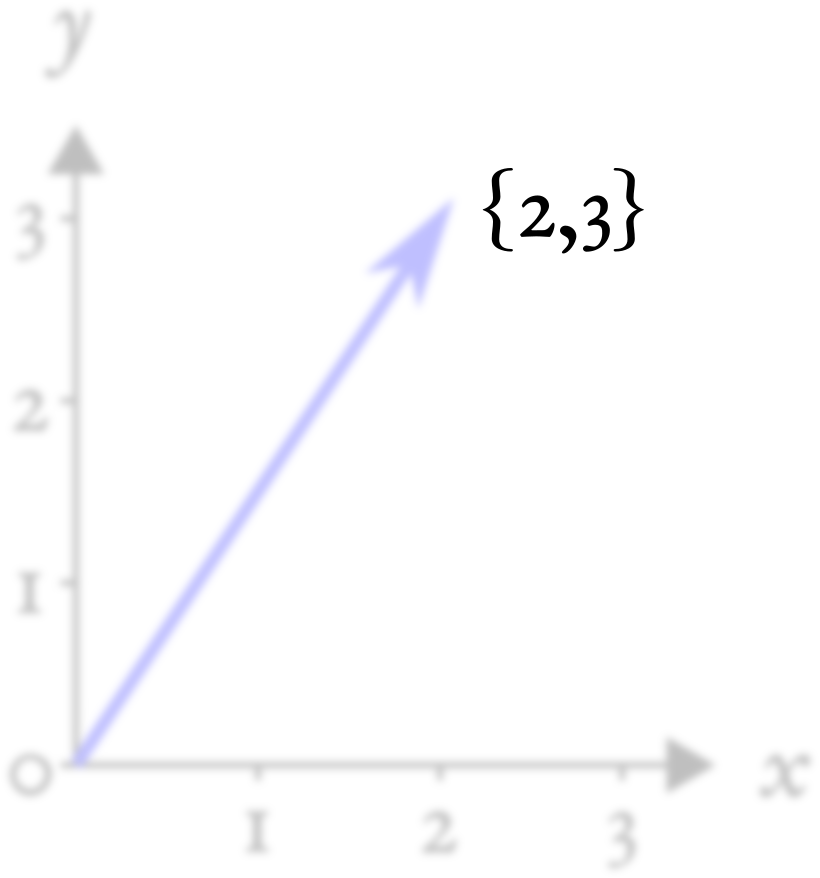
\includegraphics[width=4.16667in,height=\textheight]{images/coord_vector_blur.png}

На самом деле, мы уже работали с векторами в R, но, возможно, вы об этом
даже не догадывались. Дело в том, что в R нет как таковых скалярных
(т.е. одиночных) значений, \textbf{есть вектора длиной 1}. Такие дела!

Чтобы создать вектор из нескольких значений, нужно воспользоваться
функцией \texttt{c()}:

\begin{Shaded}
\begin{Highlighting}[]
\FunctionTok{c}\NormalTok{(}\DecValTok{4}\NormalTok{, }\DecValTok{8}\NormalTok{, }\DecValTok{15}\NormalTok{, }\DecValTok{16}\NormalTok{, }\DecValTok{23}\NormalTok{, }\DecValTok{42}\NormalTok{)}
\end{Highlighting}
\end{Shaded}

\begin{verbatim}
[1]  4  8 15 16 23 42
\end{verbatim}

\begin{Shaded}
\begin{Highlighting}[]
\FunctionTok{c}\NormalTok{(}\StringTok{"Hey"}\NormalTok{, }\StringTok{"Hey"}\NormalTok{, }\StringTok{"Ho"}\NormalTok{)}
\end{Highlighting}
\end{Shaded}

\begin{verbatim}
[1] "Hey" "Hey" "Ho" 
\end{verbatim}

\begin{Shaded}
\begin{Highlighting}[]
\FunctionTok{c}\NormalTok{(}\ConstantTok{TRUE}\NormalTok{, }\ConstantTok{FALSE}\NormalTok{)}
\end{Highlighting}
\end{Shaded}

\begin{verbatim}
[1]  TRUE FALSE
\end{verbatim}

\begin{tcolorbox}[enhanced jigsaw, leftrule=.75mm, toprule=.15mm, left=2mm, breakable, arc=.35mm, rightrule=.15mm, colback=white, opacityback=0, bottomrule=.15mm]

\textbf{\emph{Осторожно:} ошибка с кириллической ``с''}\vspace{2mm}

Одна из самых мерзких и раздражающих причин ошибок в коде -- это
использование \texttt{с} из кириллицы вместо \texttt{c} из латиницы.
Видите разницу? И я не вижу. А R видит. И об этом сообщает:

\begin{Shaded}
\begin{Highlighting}[]
\NormalTok{с(}\DecValTok{3}\NormalTok{, }\DecValTok{4}\NormalTok{, }\DecValTok{5}\NormalTok{)}
\end{Highlighting}
\end{Shaded}

\begin{verbatim}
Error in с(3, 4, 5): could not find function "с"
\end{verbatim}

\end{tcolorbox}

Для создания числовых векторов есть удобный оператор \texttt{:}.

\begin{Shaded}
\begin{Highlighting}[]
\DecValTok{1}\SpecialCharTok{:}\DecValTok{10}
\end{Highlighting}
\end{Shaded}

\begin{verbatim}
 [1]  1  2  3  4  5  6  7  8  9 10
\end{verbatim}

\begin{Shaded}
\begin{Highlighting}[]
\DecValTok{5}\SpecialCharTok{:{-}}\DecValTok{3}
\end{Highlighting}
\end{Shaded}

\begin{verbatim}
[1]  5  4  3  2  1  0 -1 -2 -3
\end{verbatim}

Этот оператор создает вектор от первого числа до второго с шагом 1. Вы
не представляете, как часто эта штука нам пригодится\ldots{} Если же
нужно сделать вектор с другим шагом, то есть функция \texttt{seq()}:

\begin{Shaded}
\begin{Highlighting}[]
\FunctionTok{seq}\NormalTok{(}\DecValTok{10}\NormalTok{, }\DecValTok{100}\NormalTok{, }\AttributeTok{by =} \DecValTok{10}\NormalTok{)}
\end{Highlighting}
\end{Shaded}

\begin{verbatim}
 [1]  10  20  30  40  50  60  70  80  90 100
\end{verbatim}

Кроме того, можно задавать не шаг, а длину вектора. Тогда функция
\texttt{seq()} сама посчитает шаг:

\begin{Shaded}
\begin{Highlighting}[]
\FunctionTok{seq}\NormalTok{(}\DecValTok{1}\NormalTok{, }\DecValTok{13}\NormalTok{, }\AttributeTok{length.out =} \DecValTok{4}\NormalTok{)}
\end{Highlighting}
\end{Shaded}

\begin{verbatim}
[1]  1  5  9 13
\end{verbatim}

Другая функция -- \texttt{rep()} -- позволяет создавать вектора с
повторяющимися значениями. Первый аргумент -- значение, которое нужно
повторять, а второй аргумент -- сколько раз повторять.

\begin{Shaded}
\begin{Highlighting}[]
\FunctionTok{rep}\NormalTok{(}\DecValTok{1}\NormalTok{, }\DecValTok{5}\NormalTok{)}
\end{Highlighting}
\end{Shaded}

\begin{verbatim}
[1] 1 1 1 1 1
\end{verbatim}

И первый, и второй аргумент могут быть векторами! Если второй агрумент
-- вектор такой же длины, то каждое значение первого вектора будет
повторено соответствующее количество раз из второго вектора.

\begin{Shaded}
\begin{Highlighting}[]
\FunctionTok{rep}\NormalTok{(}\DecValTok{1}\SpecialCharTok{:}\DecValTok{3}\NormalTok{, }\DecValTok{3}\NormalTok{)}
\end{Highlighting}
\end{Shaded}

\begin{verbatim}
[1] 1 2 3 1 2 3 1 2 3
\end{verbatim}

\begin{Shaded}
\begin{Highlighting}[]
\FunctionTok{rep}\NormalTok{(}\DecValTok{1}\SpecialCharTok{:}\DecValTok{3}\NormalTok{, }\FunctionTok{c}\NormalTok{(}\DecValTok{10}\NormalTok{, }\DecValTok{2}\NormalTok{, }\DecValTok{30}\NormalTok{))}
\end{Highlighting}
\end{Shaded}

\begin{verbatim}
 [1] 1 1 1 1 1 1 1 1 1 1 2 2 3 3 3 3 3 3 3 3 3 3 3 3 3 3 3 3 3 3 3 3 3 3 3 3 3 3
[39] 3 3 3 3
\end{verbatim}

Еще можно объединять вектора (что мы, по сути, и делали, просто с
векторами длиной 1):

\begin{Shaded}
\begin{Highlighting}[]
\NormalTok{v1 }\OtherTok{\textless{}{-}} \FunctionTok{c}\NormalTok{(}\StringTok{"Hey"}\NormalTok{, }\StringTok{"Ho"}\NormalTok{)}
\NormalTok{v2 }\OtherTok{\textless{}{-}} \FunctionTok{c}\NormalTok{(}\StringTok{"Let\textquotesingle{}s"}\NormalTok{, }\StringTok{"Go!"}\NormalTok{)}
\FunctionTok{c}\NormalTok{(v1, v2)}
\end{Highlighting}
\end{Shaded}

\begin{verbatim}
[1] "Hey"   "Ho"    "Let's" "Go!"  
\end{verbatim}

Очень многие функции в R работают именно с векторами. Например, функции
\texttt{sum()} (считает сумму значений вектора) и \texttt{mean()}
(считает среднее арифметическое всех значений в векторе):

\begin{Shaded}
\begin{Highlighting}[]
\FunctionTok{sum}\NormalTok{(}\DecValTok{1}\SpecialCharTok{:}\DecValTok{10}\NormalTok{)}
\end{Highlighting}
\end{Shaded}

\begin{verbatim}
[1] 55
\end{verbatim}

\begin{Shaded}
\begin{Highlighting}[]
\FunctionTok{mean}\NormalTok{(}\DecValTok{1}\SpecialCharTok{:}\DecValTok{10}\NormalTok{)}
\end{Highlighting}
\end{Shaded}

\begin{verbatim}
[1] 5.5
\end{verbatim}

\hypertarget{sec-coercion}{%
\section{Приведение типов}\label{sec-coercion}}

Что будет, если вы объедините два вектора с значениями разных типов?
Ошибка?

Мы уже обсуждали, что в обычных векторах (\emph{atomic} векторах) может
быть только один тип данных. В некоторых языках программирования при
операции с данными разных типов мы бы получили ошибку. А вот в R при
несовпадении типов произойдет попытка привести типы к ``общему
знаменателю'', то есть конвертировать данные в более ``широкий'' тип (а
иногда -- более ``узкий'' тип, если того требует функция).

Например:

\begin{Shaded}
\begin{Highlighting}[]
\FunctionTok{c}\NormalTok{(}\ConstantTok{FALSE}\NormalTok{, }\DecValTok{2}\NormalTok{)}
\end{Highlighting}
\end{Shaded}

\begin{verbatim}
[1] 0 2
\end{verbatim}

\texttt{FALSE} превратился в \texttt{0} (а \texttt{TRUE} превратился бы
в \texttt{1}), чтобы оба значения можно было объединить в вектор. То же
самое произошло бы в случае операций с векторами:

\begin{Shaded}
\begin{Highlighting}[]
\DecValTok{2} \SpecialCharTok{+} \ConstantTok{TRUE}
\end{Highlighting}
\end{Shaded}

\begin{verbatim}
[1] 3
\end{verbatim}

Это называется \textbf{неявным приведением типов (implicit coercion)}.

Вот более сложный пример:

\begin{Shaded}
\begin{Highlighting}[]
\FunctionTok{c}\NormalTok{(}\ConstantTok{TRUE}\NormalTok{, }\DecValTok{3}\NormalTok{, }\StringTok{"hi"}\NormalTok{)}
\end{Highlighting}
\end{Shaded}

\begin{verbatim}
[1] "TRUE" "3"    "hi"  
\end{verbatim}

Здесь все значения были приведены сразу к строковому типу данных.

\begin{tcolorbox}[enhanced jigsaw, leftrule=.75mm, toprule=.15mm, left=2mm, breakable, arc=.35mm, rightrule=.15mm, colback=white, opacityback=0, bottomrule=.15mm]

\textbf{Время мемов}\vspace{2mm}

\begin{figure}[H]

{\centering 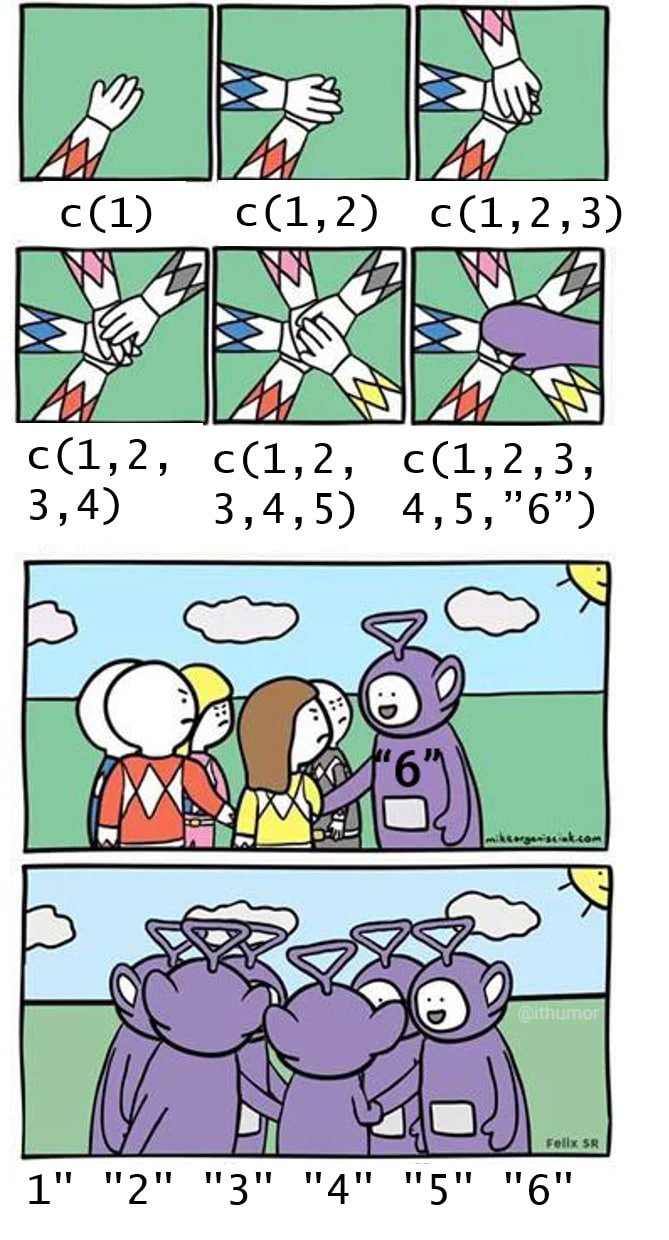
\includegraphics[width=0.56\textwidth,height=\textheight]{images/013-vector_coercion.jpeg}

}

\end{figure}

\end{tcolorbox}

У R есть иерархия приведения типов:

\texttt{NULL\ \textless{}\ raw\ \textless{}\ logical\ \textless{}\ integer\ \textless{}\ double\ \textless{}\ complex\ \textless{}\ character\ \textless{}\ list\ \textless{}\ expression}.

Мы из этого списка еще многого не знаем, сейчас важно запомнить, что
логические данные -- \texttt{FALSE} и \texttt{TRUE} -- превращаются в
\texttt{0} и \texttt{1} соответственно, а \texttt{0} и \texttt{1} в
строчки \texttt{"0"} и \texttt{"1"}.

Если Вы боитесь полагаться на приведение типов, то можете
воспользоваться функциями \texttt{as.нужныйтипданных()} для явного
приведения типов (\textbf{explicit coercion}):

\begin{Shaded}
\begin{Highlighting}[]
\FunctionTok{as.numeric}\NormalTok{(}\FunctionTok{c}\NormalTok{(}\ConstantTok{TRUE}\NormalTok{, }\ConstantTok{FALSE}\NormalTok{, }\ConstantTok{FALSE}\NormalTok{))}
\end{Highlighting}
\end{Shaded}

\begin{verbatim}
[1] 1 0 0
\end{verbatim}

\begin{Shaded}
\begin{Highlighting}[]
\FunctionTok{as.character}\NormalTok{(}\FunctionTok{as.numeric}\NormalTok{(}\FunctionTok{c}\NormalTok{(}\ConstantTok{TRUE}\NormalTok{, }\ConstantTok{FALSE}\NormalTok{, }\ConstantTok{FALSE}\NormalTok{)))}
\end{Highlighting}
\end{Shaded}

\begin{verbatim}
[1] "1" "0" "0"
\end{verbatim}

Можно превращать и обратно, например, строковые значения в числовые.
Если среди числа встретится буква или другой неподходящий знак, то мы
получим предупреждение \texttt{NA} -- пропущенное значение (мы очень
скоро научимся с ними работать, см. Глава~\ref{sec-about}).

\begin{Shaded}
\begin{Highlighting}[]
\FunctionTok{as.numeric}\NormalTok{(}\FunctionTok{c}\NormalTok{(}\StringTok{"1"}\NormalTok{, }\StringTok{"2"}\NormalTok{, }\StringTok{"три"}\NormalTok{))}
\end{Highlighting}
\end{Shaded}

\begin{verbatim}
Warning: NAs introduced by coercion
\end{verbatim}

\begin{verbatim}
[1]  1  2 NA
\end{verbatim}

\begin{tcolorbox}[enhanced jigsaw, leftrule=.75mm, toprule=.15mm, left=2mm, breakable, arc=.35mm, rightrule=.15mm, colback=white, opacityback=0, bottomrule=.15mm]

\textbf{\emph{Полезное:} подсчет количества и доли}\vspace{2mm}

Один из распространенных примеров использования неявного приведения
типов -- использования функций \texttt{sum()} и \texttt{mean()} для
подсчета в логическом векторе количества и доли \texttt{TRUE}
соответственно. Мы будем много раз пользоваться этим приемом в
дальнейшем!

\end{tcolorbox}

\hypertarget{sec-vector_op}{%
\section{Векторизация}\label{sec-vector_op}}

Все те арифметические операторы, что мы использовали ранее, можно
использовать с векторами одинаковой длины:

\begin{Shaded}
\begin{Highlighting}[]
\NormalTok{n }\OtherTok{\textless{}{-}} \DecValTok{1}\SpecialCharTok{:}\DecValTok{4}
\NormalTok{m }\OtherTok{\textless{}{-}} \DecValTok{4}\SpecialCharTok{:}\DecValTok{1}
\NormalTok{n }\SpecialCharTok{+}\NormalTok{ m}
\end{Highlighting}
\end{Shaded}

\begin{verbatim}
[1] 5 5 5 5
\end{verbatim}

\begin{Shaded}
\begin{Highlighting}[]
\NormalTok{n }\SpecialCharTok{{-}}\NormalTok{ m}
\end{Highlighting}
\end{Shaded}

\begin{verbatim}
[1] -3 -1  1  3
\end{verbatim}

\begin{Shaded}
\begin{Highlighting}[]
\NormalTok{n }\SpecialCharTok{*}\NormalTok{ m}
\end{Highlighting}
\end{Shaded}

\begin{verbatim}
[1] 4 6 6 4
\end{verbatim}

\begin{Shaded}
\begin{Highlighting}[]
\NormalTok{n }\SpecialCharTok{/}\NormalTok{ m}
\end{Highlighting}
\end{Shaded}

\begin{verbatim}
[1] 0.2500000 0.6666667 1.5000000 4.0000000
\end{verbatim}

\begin{Shaded}
\begin{Highlighting}[]
\NormalTok{n }\SpecialCharTok{\^{}}\NormalTok{ m }\SpecialCharTok{+}\NormalTok{ m }\SpecialCharTok{*}\NormalTok{ (n }\SpecialCharTok{{-}}\NormalTok{ m)}
\end{Highlighting}
\end{Shaded}

\begin{verbatim}
[1] -11   5  11   7
\end{verbatim}

Если применить операторы на двух векторах одинаковой длины, то мы
получим результат поэлементного применения оператора к двум векторам.
Это называется \textbf{векторизацией} (\textbf{vectorization}).

\begin{quote}
Если после какого-нибудь MATLAB Вы привыкли, что по умолчанию операторы
работают по правилам линейной алгебры и \texttt{m\ *\ n} будет давать
скалярное произведение (\emph{dot product}), то снова нет. Для
скалярного произведения нужно использовать операторы с \texttt{\%} по
краям:
\end{quote}

\begin{Shaded}
\begin{Highlighting}[]
\NormalTok{n }\SpecialCharTok{\%*\%}\NormalTok{ m}
\end{Highlighting}
\end{Shaded}

\begin{verbatim}
     [,1]
[1,]   20
\end{verbatim}

\begin{quote}
Абсолютно так же и с операциями с матрицами в R, хотя про матрицы будет
немного позже.
\end{quote}

В принципе, большинство функций в R, которые работают с отдельными
значениями, так же хорошо работают и с целыми векторами. Скажем, если вы
хотите извлечь корень из нескольких чисел, то для этого не нужны никакие
циклы (как это обычно делается во многих других языках
программирования). Можно просто ``скормить'' вектор функции и получить
результат применения функции к каждому элементу вектора:

\begin{Shaded}
\begin{Highlighting}[]
\FunctionTok{sqrt}\NormalTok{(}\DecValTok{1}\SpecialCharTok{:}\DecValTok{10}\NormalTok{)}
\end{Highlighting}
\end{Shaded}

\begin{verbatim}
 [1] 1.000000 1.414214 1.732051 2.000000 2.236068 2.449490 2.645751 2.828427
 [9] 3.000000 3.162278
\end{verbatim}

Таких векторизованных функций в R очень много. Многие из них написаны на
более низкоуровневых языках программирования (C, C++, FORTRAN), за счет
чего использование таких функций приводит не только к более элегантному,
лаконичному, но и к более быстрому коду.

\begin{quote}
Векторизация в R -- это очень важная фишка, которая отличает этот язык
программирования от многих других. Если вы уже имеете опыт
программирования на другом языке, то вам во многих задачах захочется
использовать циклы типа \texttt{for} и \texttt{while} @ref(for). Не
спешите этого делать! В очень многих случаях циклы можно заменить
векторизацией. Тем не менее, векторизация -- это не единственный способ
избавить от циклов типа \texttt{for} и \texttt{while} @ref(apply).
\end{quote}

\hypertarget{sec-recycling}{%
\section{Ресайклинг}\label{sec-recycling}}

Допустим мы хотим совершить какую-нибудь операцию с двумя векторами. Как
мы убедились, с этим обычно нет никаких проблем, если они совпадают по
длине. А что если вектора не совпадают по длине? Ничего страшного! Здесь
будет работать правило \textbf{ресайклинга} (\emph{правило
переписывания, recycling rule}). Это означает, что если мы делаем
операцию на двух векторах разной длины, то если короткий вектор кратен
по длине длинному, короткий вектор будет повторяться необходимое
количество раз:

\begin{Shaded}
\begin{Highlighting}[]
\NormalTok{n }\OtherTok{\textless{}{-}} \DecValTok{1}\SpecialCharTok{:}\DecValTok{4}
\NormalTok{m }\OtherTok{\textless{}{-}} \DecValTok{1}\SpecialCharTok{:}\DecValTok{2}
\NormalTok{n }\SpecialCharTok{*}\NormalTok{ m}
\end{Highlighting}
\end{Shaded}

\begin{verbatim}
[1] 1 4 3 8
\end{verbatim}

А что будет, если совершать операции с вектором и отдельным значением?
Можно считать это частным случаем ресайклинга: короткий вектор длиной 1
будет повторятся столько раз, сколько нужно, чтобы он совпадал по длине
с длинным:

\begin{Shaded}
\begin{Highlighting}[]
\NormalTok{n }\SpecialCharTok{*} \DecValTok{2}
\end{Highlighting}
\end{Shaded}

\begin{verbatim}
[1] 2 4 6 8
\end{verbatim}

Если же меньший вектор не кратен большему (например, один из них длиной
3, а другой длиной 4), то R посчитает результат, но выдаст
предупреждение.

\begin{Shaded}
\begin{Highlighting}[]
\NormalTok{n }\SpecialCharTok{+} \FunctionTok{c}\NormalTok{(}\DecValTok{3}\NormalTok{,}\DecValTok{4}\NormalTok{,}\DecValTok{5}\NormalTok{)}
\end{Highlighting}
\end{Shaded}

\begin{verbatim}
Warning in n + c(3, 4, 5): longer object length is not a multiple of shorter
object length
\end{verbatim}

\begin{verbatim}
[1] 4 6 8 7
\end{verbatim}

Проблема в том, что эти предупреждения могут в неожиданный момент стать
причиной ошибок. Поэтому
\href{https://stackoverflow.com/questions/6555651/under-what-circumstances-does-r-recycle}{не
стоит полагаться} на ресайклинг некратных по длине векторов. А вот
ресайклинг кратных по длине векторов -- это очень удобная штука, которая
используется очень часто.

\hypertarget{sec-index_atomic}{%
\section{Индексирование векторов}\label{sec-index_atomic}}

Итак, мы подошли к одному из самых сложных моментов. И одному из
основных. От того, как хорошо вы научись с этим работать, зависит весь
ваш дальнейший успех на R-поприще!

Речь пойдет об \textbf{индексировании} векторов. Задача, которую Вам
придется решать каждые пять минут работы в R -- как выбрать из вектора
(или же списка, матрицы и датафрейма) какую-то его часть. Для этого
используются квадратные скобочки \texttt{{[}{]}} (не круглые -- они для
функций!).

Самое простое -- индексировать по номеру индекса, т.е. порядку значения
в векторе.

\begin{Shaded}
\begin{Highlighting}[]
\NormalTok{n }\OtherTok{\textless{}{-}} \FunctionTok{c}\NormalTok{(}\DecValTok{0}\NormalTok{, }\DecValTok{1}\NormalTok{, }\DecValTok{1}\NormalTok{, }\DecValTok{2}\NormalTok{, }\DecValTok{3}\NormalTok{, }\DecValTok{5}\NormalTok{, }\DecValTok{8}\NormalTok{, }\DecValTok{13}\NormalTok{, }\DecValTok{21}\NormalTok{, }\DecValTok{34}\NormalTok{)}
\NormalTok{n[}\DecValTok{1}\NormalTok{]}
\end{Highlighting}
\end{Shaded}

\begin{verbatim}
[1] 0
\end{verbatim}

\begin{Shaded}
\begin{Highlighting}[]
\NormalTok{n[}\DecValTok{10}\NormalTok{]}
\end{Highlighting}
\end{Shaded}

\begin{verbatim}
[1] 34
\end{verbatim}

\begin{quote}
Если вы знакомы с другими языками программирования (не MATLAB, там все
так же) и уже научились думать, что индексация с 0 -- это очень удобно и
очень правильно (ну или просто свыклись с этим), то в R вам придется
переучиться обратно. Здесь первый индекс -- это 1, а последний равен
длине вектора -- ее можно узнать с помощью функции \texttt{length()}. С
обоих сторон индексы берутся включительно.
\end{quote}

С помощью индексирования можно не только вытаскивать имеющиеся значения
в векторе, но и присваивать им новые:

\begin{Shaded}
\begin{Highlighting}[]
\NormalTok{n[}\DecValTok{3}\NormalTok{] }\OtherTok{\textless{}{-}} \DecValTok{20}
\NormalTok{n}
\end{Highlighting}
\end{Shaded}

\begin{verbatim}
 [1]  0  1 20  2  3  5  8 13 21 34
\end{verbatim}

Конечно, можно использовать целые векторы для индексирования:

\begin{Shaded}
\begin{Highlighting}[]
\NormalTok{n[}\DecValTok{4}\SpecialCharTok{:}\DecValTok{7}\NormalTok{]}
\end{Highlighting}
\end{Shaded}

\begin{verbatim}
[1] 2 3 5 8
\end{verbatim}

\begin{Shaded}
\begin{Highlighting}[]
\NormalTok{n[}\DecValTok{10}\SpecialCharTok{:}\DecValTok{1}\NormalTok{]}
\end{Highlighting}
\end{Shaded}

\begin{verbatim}
 [1] 34 21 13  8  5  3  2 20  1  0
\end{verbatim}

\begin{Shaded}
\begin{Highlighting}[]
\NormalTok{n[}\DecValTok{4}\SpecialCharTok{:}\DecValTok{6}\NormalTok{] }\OtherTok{\textless{}{-}} \DecValTok{0}
\NormalTok{n}
\end{Highlighting}
\end{Shaded}

\begin{verbatim}
 [1]  0  1 20  0  0  0  8 13 21 34
\end{verbatim}

Индексирование с минусом выдаст вам все значения вектора кроме
выбранных:

\begin{Shaded}
\begin{Highlighting}[]
\NormalTok{n[}\SpecialCharTok{{-}}\DecValTok{1}\NormalTok{]}
\end{Highlighting}
\end{Shaded}

\begin{verbatim}
[1]  1 20  0  0  0  8 13 21 34
\end{verbatim}

\begin{Shaded}
\begin{Highlighting}[]
\NormalTok{n[}\FunctionTok{c}\NormalTok{(}\SpecialCharTok{{-}}\DecValTok{4}\NormalTok{, }\SpecialCharTok{{-}}\DecValTok{5}\NormalTok{)]}
\end{Highlighting}
\end{Shaded}

\begin{verbatim}
[1]  0  1 20  0  8 13 21 34
\end{verbatim}

Минус здесь ``выключает'' выбранные значения из вектора, а не означает
отсчет с конца как в Python.

Более того, можно использовать логический вектор для индексирования. В
этом случае нужен логический вектор такой же длины:

\begin{Shaded}
\begin{Highlighting}[]
\NormalTok{n[}\FunctionTok{c}\NormalTok{(}\ConstantTok{TRUE}\NormalTok{, }\ConstantTok{FALSE}\NormalTok{, }\ConstantTok{TRUE}\NormalTok{, }\ConstantTok{FALSE}\NormalTok{, }\ConstantTok{TRUE}\NormalTok{, }\ConstantTok{FALSE}\NormalTok{, }\ConstantTok{TRUE}\NormalTok{, }\ConstantTok{FALSE}\NormalTok{, }\ConstantTok{TRUE}\NormalTok{, }\ConstantTok{FALSE}\NormalTok{)]}
\end{Highlighting}
\end{Shaded}

\begin{verbatim}
[1]  0 20  0  8 21
\end{verbatim}

Логический вектор работает здесь как фильтр: пропускает только те
значения, где на соответствующей позиции в логическом векторе для
индексирования содержится \texttt{TRUE}, и не пропускает те значения,
где на соответствующей позиции в логическом векторе для индексирования
содержится \texttt{FALSE}.

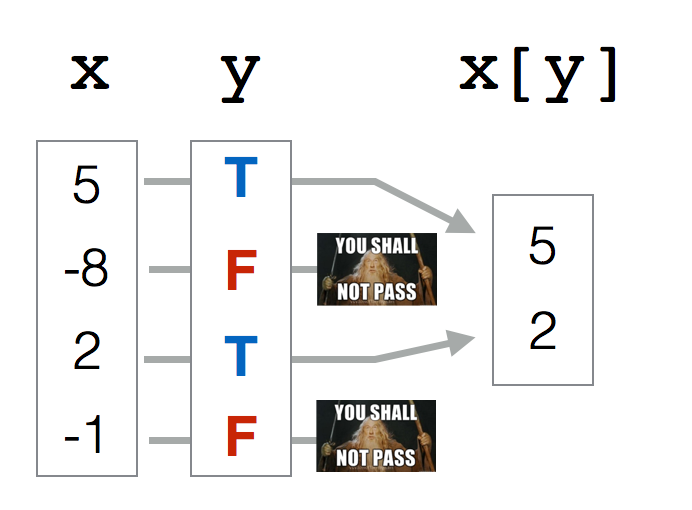
\includegraphics[width=4.16667in,height=\textheight]{images/indexgandolf.png}

Ну а если эти два вектора (исходный вектор и логический вектор индексов)
не равны по длине, то тут будет снова работать правило ресайклинга!

\begin{Shaded}
\begin{Highlighting}[]
\NormalTok{n[}\FunctionTok{c}\NormalTok{(}\ConstantTok{TRUE}\NormalTok{, }\ConstantTok{FALSE}\NormalTok{)] }\CommentTok{\#то же самое {-} recycling rule!}
\end{Highlighting}
\end{Shaded}

\begin{verbatim}
[1]  0 20  0  8 21
\end{verbatim}

Есть еще один способ индексирования векторов, но он несколько более
редкий: индексирование по имени. Дело в том, что для значений векторов
можно (но не обязательно) присваивать имена:

\begin{Shaded}
\begin{Highlighting}[]
\NormalTok{my\_named\_vector }\OtherTok{\textless{}{-}} \FunctionTok{c}\NormalTok{(}\AttributeTok{first =} \DecValTok{1}\NormalTok{,}
                     \AttributeTok{second =} \DecValTok{2}\NormalTok{,}
                     \AttributeTok{third =} \DecValTok{3}\NormalTok{)}
\NormalTok{my\_named\_vector[}\StringTok{\textquotesingle{}first\textquotesingle{}}\NormalTok{]}
\end{Highlighting}
\end{Shaded}

\begin{verbatim}
first 
    1 
\end{verbatim}

А еще можно ``вытаскивать'' имена из вектора с помощью функции
\texttt{names()} и присваивать таким образом новые имена.

\begin{Shaded}
\begin{Highlighting}[]
\NormalTok{d }\OtherTok{\textless{}{-}} \DecValTok{1}\SpecialCharTok{:}\DecValTok{4}
\FunctionTok{names}\NormalTok{(d) }\OtherTok{\textless{}{-}}\NormalTok{ letters[}\DecValTok{1}\SpecialCharTok{:}\DecValTok{4}\NormalTok{]}
\FunctionTok{names}\NormalTok{(d)}
\end{Highlighting}
\end{Shaded}

\begin{verbatim}
[1] "a" "b" "c" "d"
\end{verbatim}

\begin{Shaded}
\begin{Highlighting}[]
\NormalTok{d[}\StringTok{"a"}\NormalTok{]}
\end{Highlighting}
\end{Shaded}

\begin{verbatim}
a 
1 
\end{verbatim}

\begin{quote}
\texttt{letters} -- это ``зашитая'' в R константа -- вектор букв от a до
z. Иногда это очень удобно! Кроме того, есть константа \texttt{LETTERS}
-- то же самое, но заглавными буквами. А еще в R есть названия месяцев
на английском и числовая константа \texttt{pi}.
\end{quote}

Вернемся к нашему вектору \texttt{n} и посчитаем его среднее с помощью
функции \texttt{mean()}:

\begin{Shaded}
\begin{Highlighting}[]
\FunctionTok{mean}\NormalTok{(n)}
\end{Highlighting}
\end{Shaded}

\begin{verbatim}
[1] 9.7
\end{verbatim}

А как вытащить все значения, которые больше среднего?

Сначала получим логический вектор -- какие значения больше среднего:

\begin{Shaded}
\begin{Highlighting}[]
\NormalTok{larger }\OtherTok{\textless{}{-}}\NormalTok{ n }\SpecialCharTok{\textgreater{}} \FunctionTok{mean}\NormalTok{(n)}
\NormalTok{larger}
\end{Highlighting}
\end{Shaded}

\begin{verbatim}
 [1] FALSE FALSE  TRUE FALSE FALSE FALSE FALSE  TRUE  TRUE  TRUE
\end{verbatim}

А теперь используем его для индексирования вектора \texttt{n}:

\begin{Shaded}
\begin{Highlighting}[]
\NormalTok{n[larger]}
\end{Highlighting}
\end{Shaded}

\begin{verbatim}
[1] 20 13 21 34
\end{verbatim}

Можно все это сделать в одну строчку:

\begin{Shaded}
\begin{Highlighting}[]
\NormalTok{n[n }\SpecialCharTok{\textgreater{}} \FunctionTok{mean}\NormalTok{(n)]}
\end{Highlighting}
\end{Shaded}

\begin{verbatim}
[1] 20 13 21 34
\end{verbatim}

Предыдущая строчка отражает то, что мы будем постоянно делать в R:
вычленять (subset) из данных отдельные куски на основании разных
условий.

\hypertarget{sec-logic_vectors}{%
\section{Работа с логическими векторами}\label{sec-logic_vectors}}

На работе с логическими векторами построено очень много удобных фишек,
связанных со сравнением условий.

\begin{Shaded}
\begin{Highlighting}[]
\NormalTok{eyes }\OtherTok{\textless{}{-}} \FunctionTok{c}\NormalTok{(}\StringTok{"green"}\NormalTok{, }\StringTok{"blue"}\NormalTok{, }\StringTok{"blue"}\NormalTok{, }\StringTok{"brown"}\NormalTok{, }\StringTok{"green"}\NormalTok{, }\StringTok{"blue"}\NormalTok{)}
\end{Highlighting}
\end{Shaded}

\hypertarget{sec-logic_mean_sum}{%
\subsection{\texorpdfstring{\texttt{mean()} и \texttt{sum()} для
подсчета пропорций и количества
TRUE}{mean() и sum() для подсчета пропорций и количества TRUE}}\label{sec-logic_mean_sum}}

Уже знакомая нам функция \texttt{sum()} позволяет посчитать количество
\texttt{TRUE} в логическом векторе. Например, можно удобно посчитать
сколько раз значение \texttt{"blue"} встречается в векторе
\texttt{eyes}:

\begin{Shaded}
\begin{Highlighting}[]
\NormalTok{eyes }\SpecialCharTok{==} \StringTok{"blue"}
\end{Highlighting}
\end{Shaded}

\begin{verbatim}
[1] FALSE  TRUE  TRUE FALSE FALSE  TRUE
\end{verbatim}

\begin{Shaded}
\begin{Highlighting}[]
\FunctionTok{sum}\NormalTok{(eyes }\SpecialCharTok{==} \StringTok{"blue"}\NormalTok{)}
\end{Highlighting}
\end{Shaded}

\begin{verbatim}
[1] 3
\end{verbatim}

Функцию \texttt{mean()} можно использовать для подсчета пропорций
\texttt{TRUE} в логическом векторе.

\begin{Shaded}
\begin{Highlighting}[]
\NormalTok{eyes }\SpecialCharTok{==} \StringTok{"blue"}
\end{Highlighting}
\end{Shaded}

\begin{verbatim}
[1] FALSE  TRUE  TRUE FALSE FALSE  TRUE
\end{verbatim}

\begin{Shaded}
\begin{Highlighting}[]
\FunctionTok{mean}\NormalTok{(eyes }\SpecialCharTok{==} \StringTok{"blue"}\NormalTok{)}
\end{Highlighting}
\end{Shaded}

\begin{verbatim}
[1] 0.5
\end{verbatim}

Умножив на 100, мы получим долю выраженную в процентах:

\begin{Shaded}
\begin{Highlighting}[]
\FunctionTok{mean}\NormalTok{(eyes }\SpecialCharTok{==} \StringTok{"blue"}\NormalTok{) }\SpecialCharTok{*} \DecValTok{100}
\end{Highlighting}
\end{Shaded}

\begin{verbatim}
[1] 50
\end{verbatim}

\hypertarget{sec-all_any}{%
\subsection{\texorpdfstring{\texttt{all()} и
\texttt{any()}}{all() и any()}}\label{sec-all_any}}

Функция \texttt{all()} выдает \texttt{TRUE} только когда все значения
логического вектора на входе равны \texttt{TRUE}:

\begin{Shaded}
\begin{Highlighting}[]
\FunctionTok{all}\NormalTok{(eyes }\SpecialCharTok{==} \StringTok{"blue"}\NormalTok{)}
\end{Highlighting}
\end{Shaded}

\begin{verbatim}
[1] FALSE
\end{verbatim}

Функция \texttt{any()} выдает \texttt{TRUE} когда есть хотя бы одно
значение \texttt{TRUE}:

\begin{Shaded}
\begin{Highlighting}[]
\FunctionTok{any}\NormalTok{(eyes }\SpecialCharTok{==} \StringTok{"blue"}\NormalTok{)}
\end{Highlighting}
\end{Shaded}

\begin{verbatim}
[1] TRUE
\end{verbatim}

Вместе с оператором \texttt{!} можно получить много дополнительных
вариантов. Например, есть ли хотя бы один \texttt{FALSE} в векторе?

\begin{Shaded}
\begin{Highlighting}[]
\FunctionTok{any}\NormalTok{(}\SpecialCharTok{!}\NormalTok{eyes }\SpecialCharTok{==} \StringTok{"blue"}\NormalTok{)}
\end{Highlighting}
\end{Shaded}

\begin{verbatim}
[1] TRUE
\end{verbatim}

\begin{Shaded}
\begin{Highlighting}[]
\SpecialCharTok{!}\FunctionTok{all}\NormalTok{(eyes }\SpecialCharTok{==} \StringTok{"blue"}\NormalTok{)}
\end{Highlighting}
\end{Shaded}

\begin{verbatim}
[1] TRUE
\end{verbatim}

Все ли значения в векторе равны \texttt{FALSE}?

\begin{Shaded}
\begin{Highlighting}[]
\FunctionTok{all}\NormalTok{(}\SpecialCharTok{!}\NormalTok{eyes }\SpecialCharTok{==} \StringTok{"blue"}\NormalTok{)}
\end{Highlighting}
\end{Shaded}

\begin{verbatim}
[1] FALSE
\end{verbatim}

\begin{Shaded}
\begin{Highlighting}[]
\SpecialCharTok{!}\FunctionTok{any}\NormalTok{(eyes }\SpecialCharTok{==} \StringTok{"blue"}\NormalTok{)}
\end{Highlighting}
\end{Shaded}

\begin{verbatim}
[1] FALSE
\end{verbatim}

\hypertarget{sec-which}{%
\subsection{\texorpdfstring{Превращение логических значений в индексы:
\texttt{which()}}{Превращение логических значений в индексы: which()}}\label{sec-which}}

Как вы уже знаете, и логические векторы, и числовые вектора с индексами
могут использоваться для индексирования векторов. Иногда может
понадобиться превратить логический вектор в вектор индексов. Для этого
есть функция \texttt{which()}

\begin{Shaded}
\begin{Highlighting}[]
\FunctionTok{which}\NormalTok{(eyes }\SpecialCharTok{==} \StringTok{"blue"}\NormalTok{)}
\end{Highlighting}
\end{Shaded}

\begin{verbatim}
[1] 2 3 6
\end{verbatim}

\hypertarget{sec-in}{%
\subsection{оператор \%in\% и match()}\label{sec-in}}

Часто возникает такая задача: нужно проверить вектор на равенство с хотя
бы одним значением из другого вектора. Например, мы хотим вычленить всех
зеленоглазых и голубоглазых. Может возникнуть идея сделать так:

\begin{Shaded}
\begin{Highlighting}[]
\NormalTok{eyes[eyes }\SpecialCharTok{==} \FunctionTok{c}\NormalTok{(}\StringTok{"green"}\NormalTok{, }\StringTok{"blue"}\NormalTok{)]}
\end{Highlighting}
\end{Shaded}

\begin{verbatim}
[1] "green" "blue"  "green" "blue" 
\end{verbatim}

Перед нами самый страшный случай: результат \emph{похож} на правильный,
но не правильный! Попытайтесь самостоятельно понять почему этот ответ
неверный и что произошло на самом деле.

А на самом деле мы просто сравнили два вектора, один из которых короче
другого, следовательно, у нас сработало правило ресайклинга.

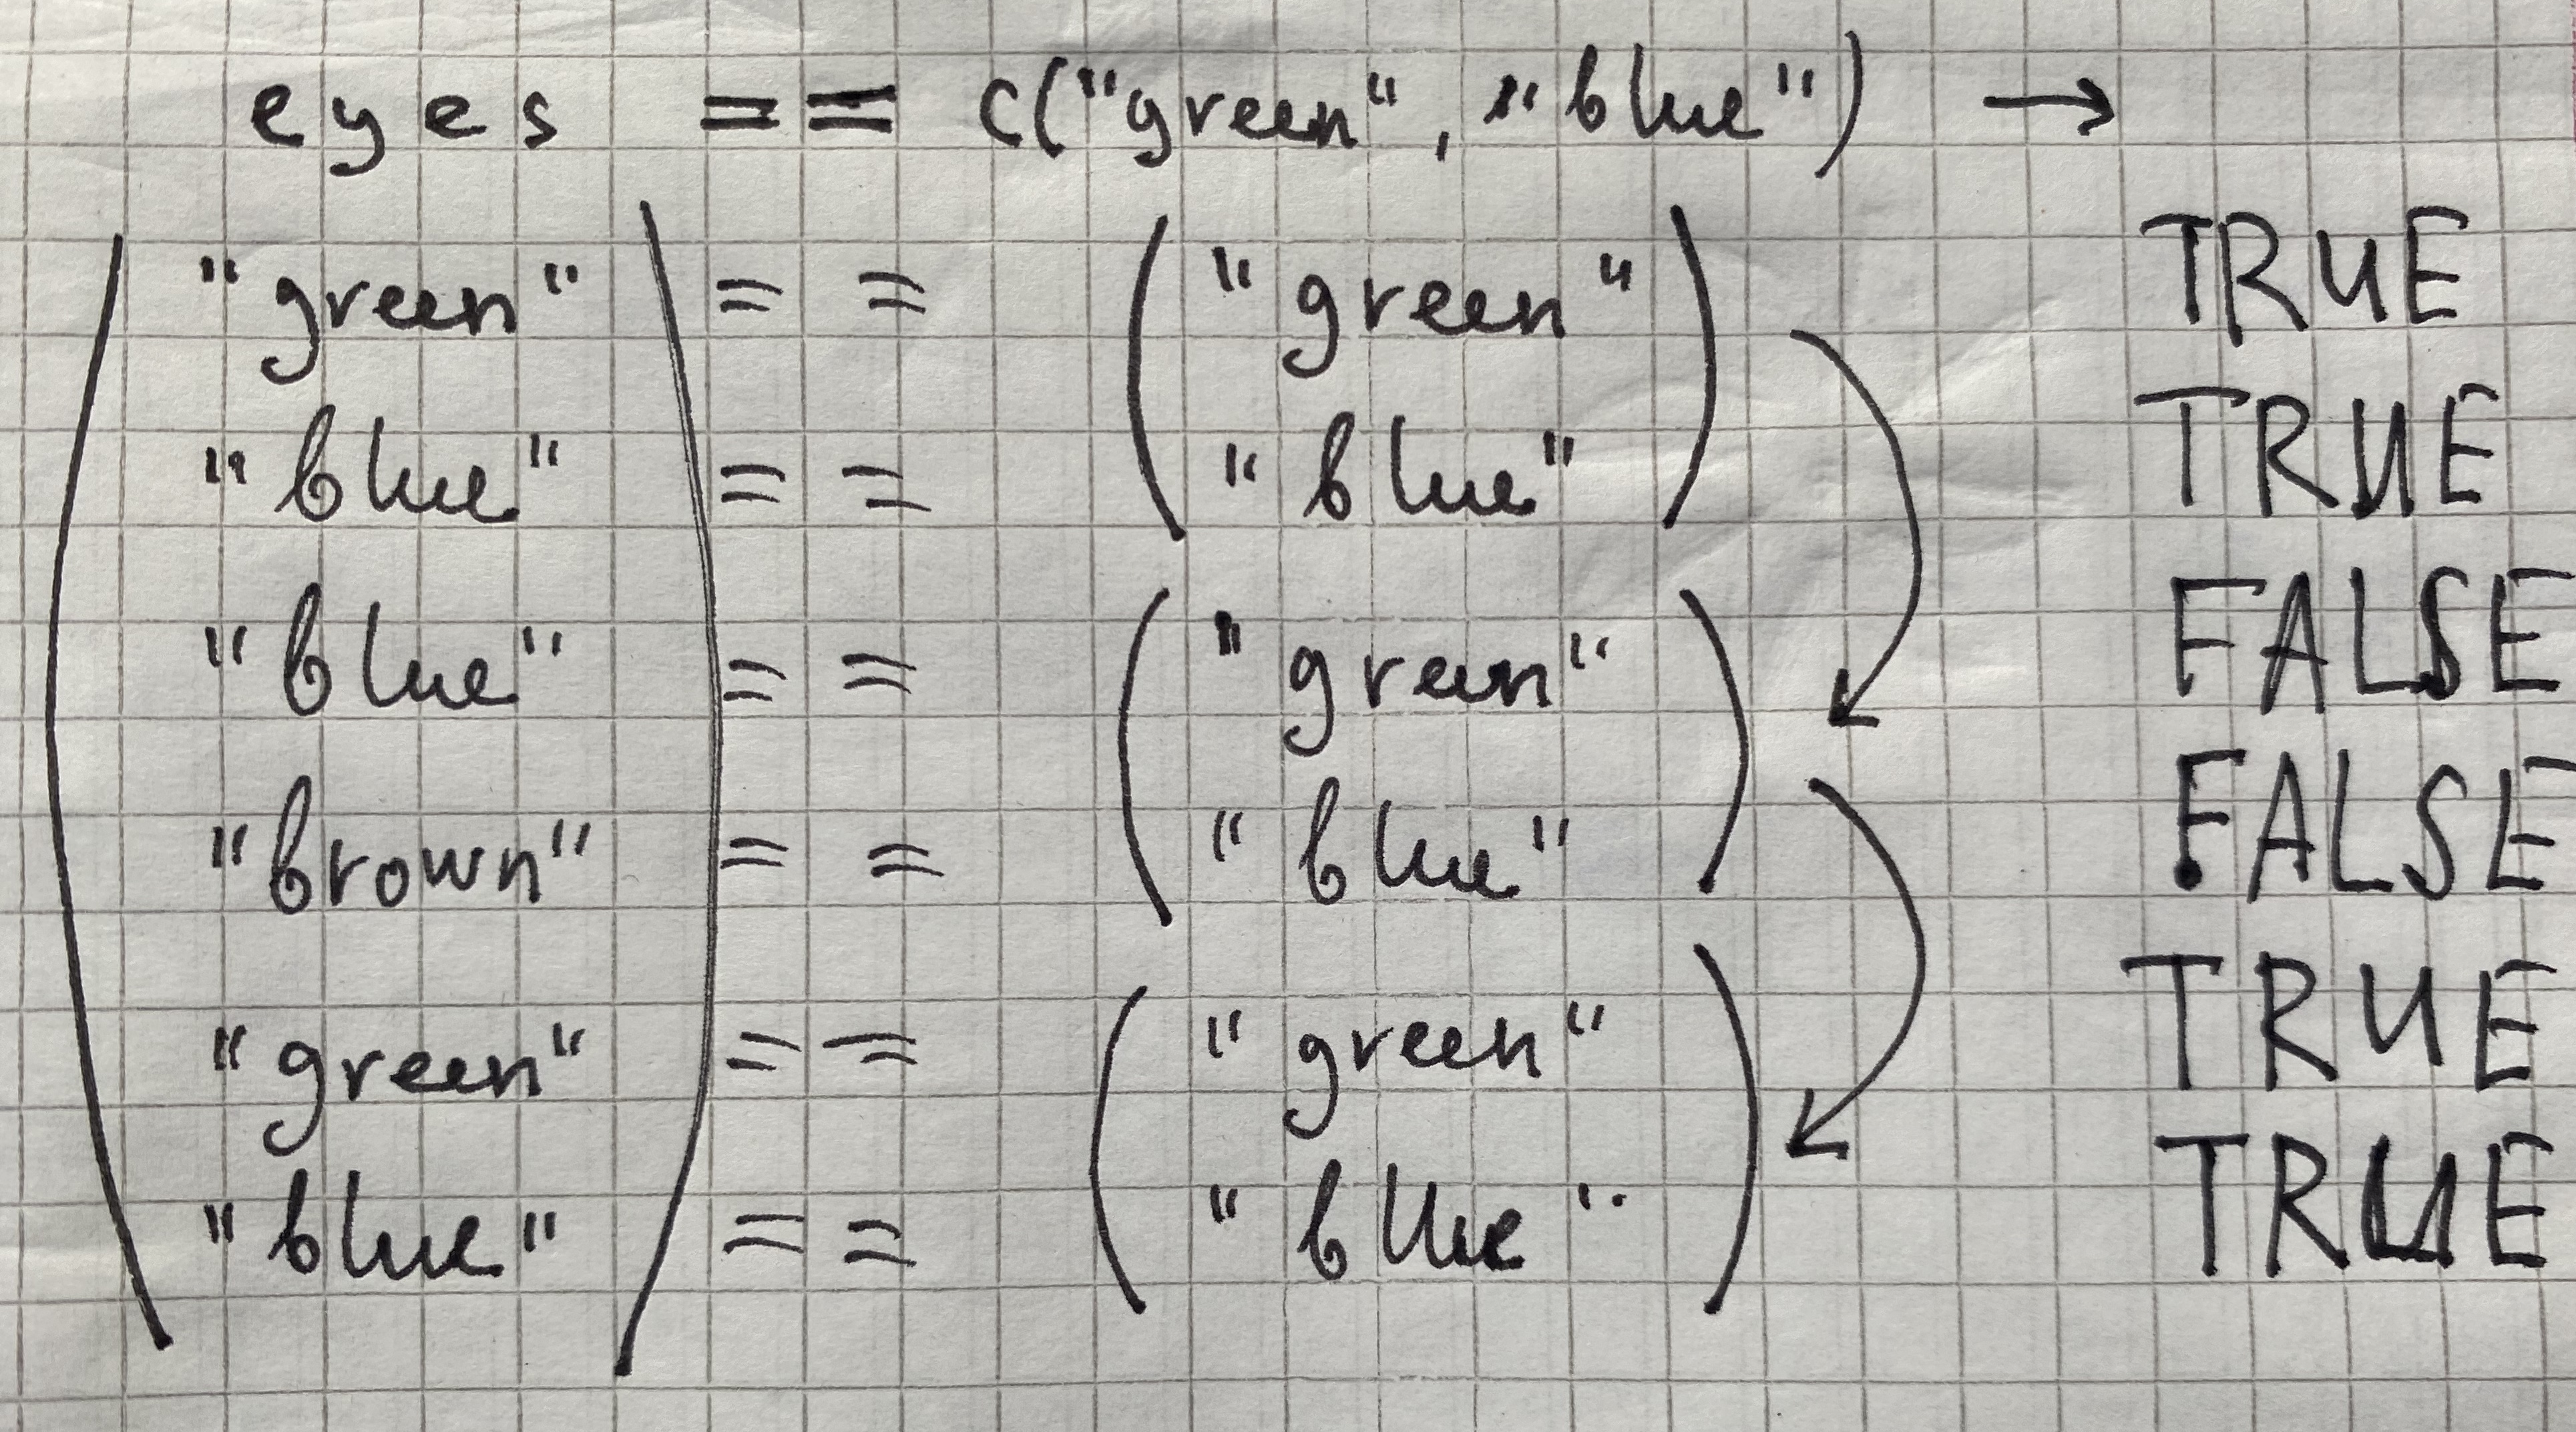
\includegraphics{images/logical_vectors_recycling.jpg}

Как мы видим, это совсем не то, что нам нужно! В данной ситуации нам
подойдет сравнение с двумя значениями вместе с логическим ИЛИ.

\begin{Shaded}
\begin{Highlighting}[]
\NormalTok{eyes[eyes }\SpecialCharTok{==} \StringTok{"green"} \SpecialCharTok{|}\NormalTok{ eyes }\SpecialCharTok{==} \StringTok{"blue"}\NormalTok{]}
\end{Highlighting}
\end{Shaded}

\begin{verbatim}
[1] "green" "blue"  "blue"  "green" "blue" 
\end{verbatim}

Однако это не очень удобно, особенно если значений больше 2. Тогда на
помощь приходит оператор \texttt{\%in\%}, который выполняет именно то,
что нам изначально нужно: выдает для каждого значения в векторе слева,
есть ли это значение среди значений вектора справа.

\begin{Shaded}
\begin{Highlighting}[]
\NormalTok{eyes[eyes }\SpecialCharTok{\%in\%} \FunctionTok{c}\NormalTok{(}\StringTok{"green"}\NormalTok{, }\StringTok{"blue"}\NormalTok{)]}
\end{Highlighting}
\end{Shaded}

\begin{verbatim}
[1] "green" "blue"  "blue"  "green" "blue" 
\end{verbatim}

\begin{tcolorbox}[enhanced jigsaw, leftrule=.75mm, toprule=.15mm, left=2mm, breakable, arc=.35mm, rightrule=.15mm, colback=white, opacityback=0, bottomrule=.15mm]

\textbf{\emph{Для продвинутых:} \texttt{match()}}\vspace{2mm}

Основное преимущество оператора \texttt{\%in\%} в его простоте и
понятности. У оператора \texttt{\%in\%} есть старший брат, более сложный
и более мощный.

Функция \texttt{match()} работает похожим образом на \texttt{\%in\%}, но
при совпадении значения в левом векторе с одним из значений в правом
выдает индекс соответствующего значения вместо \texttt{TRUE}. Если же
совпадений нет, то вместо \texttt{FALSE} функция \texttt{match()} выдает
\texttt{NA} (что можно поменять параметром \texttt{nomatch\ =}).

\begin{Shaded}
\begin{Highlighting}[]
\FunctionTok{match}\NormalTok{(eyes, }\FunctionTok{c}\NormalTok{(}\StringTok{"green"}\NormalTok{, }\StringTok{"blue"}\NormalTok{))}
\end{Highlighting}
\end{Shaded}

\begin{verbatim}
[1]  1  2  2 NA  1  2
\end{verbatim}

Зачем это может понадобиться? Во-первых, это способ соединить два набора
данных (хотя для этого есть и более подходящие инструменты), во-вторых,
так можно заменить все значения кроме выбранных заменить на \texttt{NA}
(для чего тоже есть альтернативы).

\begin{Shaded}
\begin{Highlighting}[]
\FunctionTok{c}\NormalTok{(}\StringTok{"green"}\NormalTok{, }\StringTok{"blue"}\NormalTok{)[}\FunctionTok{match}\NormalTok{(eyes, }\FunctionTok{c}\NormalTok{(}\StringTok{"green"}\NormalTok{, }\StringTok{"blue"}\NormalTok{))]}
\end{Highlighting}
\end{Shaded}

\begin{verbatim}
[1] "green" "blue"  "blue"  NA      "green" "blue" 
\end{verbatim}

\end{tcolorbox}

\hypertarget{sec-na}{%
\section{NA - пропущенные значения}\label{sec-na}}

В реальных данных у нас часто чего-то не хватает. Например, из-за
технической ошибки или невнимательности не получилось записать какое-то
измерение. Для обозначения пропущенных значений в R есть специальное
значение \texttt{NA} (расшифровывается как \emph{Not Available} -
недоступное значение). \texttt{NA} -- это не строка \texttt{"NA"}, не
\texttt{0}, не пустая строка \texttt{""} и не \texttt{FALSE}.
\texttt{NA} -- это \texttt{NA}. Большинство операций с векторами,
содержащими \texttt{NA} будут выдавать \texttt{NA}:

\begin{Shaded}
\begin{Highlighting}[]
\NormalTok{missed }\OtherTok{\textless{}{-}} \ConstantTok{NA}
\NormalTok{missed }\SpecialCharTok{==} \StringTok{"NA"}
\end{Highlighting}
\end{Shaded}

\begin{verbatim}
[1] NA
\end{verbatim}

\begin{Shaded}
\begin{Highlighting}[]
\NormalTok{missed }\SpecialCharTok{==} \StringTok{""}
\end{Highlighting}
\end{Shaded}

\begin{verbatim}
[1] NA
\end{verbatim}

\begin{Shaded}
\begin{Highlighting}[]
\NormalTok{missed }\SpecialCharTok{==} \ConstantTok{NA}
\end{Highlighting}
\end{Shaded}

\begin{verbatim}
[1] NA
\end{verbatim}

Заметьте, даже сравнение \texttt{NA} c \texttt{NA} выдает \texttt{NA}.
Это может прозвучать абсурдно: ну как же так, и то \texttt{NA}, и другое
\texttt{NA} -- это же одно и то же, они должны быть равны! Не совсем:
\texttt{NA} -- это отсутствие информации об объекте, неопределенность,
неизвестная нам величина. Если мы не знаем двух значений (т.е. имеем два
\texttt{NA}), то это еще не значит, что они равны.

Иногда наличие \texttt{NA} в данных очень бесит:

\begin{Shaded}
\begin{Highlighting}[]
\NormalTok{n[}\DecValTok{5}\NormalTok{] }\OtherTok{\textless{}{-}} \ConstantTok{NA}
\NormalTok{n}
\end{Highlighting}
\end{Shaded}

\begin{verbatim}
 [1]  0  1 20  0 NA  0  8 13 21 34
\end{verbatim}

\begin{Shaded}
\begin{Highlighting}[]
\FunctionTok{mean}\NormalTok{(n)}
\end{Highlighting}
\end{Shaded}

\begin{verbatim}
[1] NA
\end{verbatim}

Получается, что наличие \texttt{NA} ``заражает'' неопределенностью все
последующие действия. Что же делать?

Наверное, надо сравнить вектор с \texttt{NA} и исключить этих
пакостников. Давайте попробуем:

\begin{Shaded}
\begin{Highlighting}[]
\NormalTok{n }\SpecialCharTok{==} \ConstantTok{NA}
\end{Highlighting}
\end{Shaded}

\begin{verbatim}
 [1] NA NA NA NA NA NA NA NA NA NA
\end{verbatim}

Ах да, мы ведь только что узнали, что даже сравнение \texttt{NA} c
\texttt{NA} приводит к \texttt{NA}! Сначала это может показаться
нелогичным: ведь с обоих сторон \texttt{NA}, почему же тогда результат
их сравнения -- это тоже \texttt{NA}, а не \texttt{TRUE}?

Дело в том, что сравнивая две неопределенности, вы не можете установить
между ними знак равенства. Представим себе двух супергероев: Бэтмена и
Спайдермена. Допустим, мы не знаем их рост:

\begin{Shaded}
\begin{Highlighting}[]
\NormalTok{Batman }\OtherTok{\textless{}{-}} \ConstantTok{NA}
\NormalTok{Spiderman }\OtherTok{\textless{}{-}} \ConstantTok{NA}
\end{Highlighting}
\end{Shaded}

Одинаковый ли у них рост?

\begin{Shaded}
\begin{Highlighting}[]
\NormalTok{Batman }\SpecialCharTok{==}\NormalTok{ Spiderman}
\end{Highlighting}
\end{Shaded}

\begin{verbatim}
[1] NA
\end{verbatim}

Мы не знаем! Возможно, да, возможно, и нет. Поэтому у нас здесь остается
неопределенность.

Так как же избавиться от \texttt{NA} в данных? Самый простой способ --
это функция \texttt{is.na()}:

\begin{Shaded}
\begin{Highlighting}[]
\FunctionTok{is.na}\NormalTok{(n)}
\end{Highlighting}
\end{Shaded}

\begin{verbatim}
 [1] FALSE FALSE FALSE FALSE  TRUE FALSE FALSE FALSE FALSE FALSE
\end{verbatim}

Результат выполнения \texttt{is.na(n)} выдает \texttt{FALSE} на тех
позициях, где у нас числа (или другие значения), и \texttt{TRUE} там,
где у нас \texttt{NA}. Чтобы вычленить из вектора \texttt{n} все
значения кроме \texttt{NA} нам нужно, чтобы было наоборот:
\texttt{TRUE}, если это не \texttt{NA}, \texttt{FALSE}, если это
\texttt{NA}. Здесь нам понадобится логический оператор НЕ \texttt{!} (мы
его уже встречали -- см. Глава~\ref{sec-type_logical}), который
инвертирует логические значения:

\begin{Shaded}
\begin{Highlighting}[]
\NormalTok{n[}\SpecialCharTok{!}\FunctionTok{is.na}\NormalTok{(n)]}
\end{Highlighting}
\end{Shaded}

\begin{verbatim}
[1]  0  1 20  0  0  8 13 21 34
\end{verbatim}

Ура, мы можем считать среднее без \texttt{NA}!

\begin{Shaded}
\begin{Highlighting}[]
\FunctionTok{mean}\NormalTok{(n[}\SpecialCharTok{!}\FunctionTok{is.na}\NormalTok{(n)])}
\end{Highlighting}
\end{Shaded}

\begin{verbatim}
[1] 10.77778
\end{verbatim}

Теперь Вы понимаете, зачем нужно отрицание (\texttt{!})

\begin{tcolorbox}[enhanced jigsaw, leftrule=.75mm, toprule=.15mm, left=2mm, breakable, arc=.35mm, rightrule=.15mm, colback=white, opacityback=0, bottomrule=.15mm]

\textbf{\emph{Полезное:} \texttt{na.rm\ =\ TRUE}}\vspace{2mm}

Вообще, есть еще один способ посчитать среднее, если есть NA. Для этого
надо залезть в хэлп по функции \emph{mean()}:

\begin{Shaded}
\begin{Highlighting}[]
\NormalTok{?}\FunctionTok{mean}\NormalTok{()}
\end{Highlighting}
\end{Shaded}

В хэлпе мы найдем параметр \texttt{na.rm\ =}, который по умолчанию
\texttt{FALSE}. Вы знаете, что нужно делать!

\begin{Shaded}
\begin{Highlighting}[]
\FunctionTok{mean}\NormalTok{(n, }\AttributeTok{na.rm =} \ConstantTok{TRUE}\NormalTok{)}
\end{Highlighting}
\end{Shaded}

\begin{verbatim}
[1] 10.77778
\end{verbatim}

\texttt{NA} может появляться в векторах разных типов. На самом деле,
\texttt{NA} - это специальное значение в логических векторах, тогда как
в векторах других типов \texttt{NA} появляется как
\texttt{NA\_integer\_}, \texttt{NA\_real\_}, \texttt{NA\_complex\_} или
\texttt{NA\_character\_}, но R обычно сам все переводит в нужный формат
и показывает как просто \texttt{NA}. Таким образом, \texttt{NA} в
векторах разных типов -- это разные \texttt{NA}, хотя на практике эта
деталь обычно несущественна.

\end{tcolorbox}

\begin{tcolorbox}[enhanced jigsaw, leftrule=.75mm, toprule=.15mm, left=2mm, breakable, arc=.35mm, rightrule=.15mm, colback=white, opacityback=0, bottomrule=.15mm]

\textbf{\emph{Для продвинутых:} \texttt{NA} против
\texttt{NaN}}\vspace{2mm}

Кроме \texttt{NA} есть еще \texttt{NaN} -- это разные вещи. \texttt{NaN}
расшифровывается как \emph{Not a Number} и получается в результате таких
операций как \texttt{0\ /\ 0}. Тем не менее, функция \texttt{is.na()}
выдает \texttt{TRUE} на \texttt{NaN}, а вот функция \texttt{is.nan()}
выдает \texttt{TRUE} на \texttt{NaN} и \texttt{FALSE} на \texttt{NA}:

\begin{Shaded}
\begin{Highlighting}[]
\FunctionTok{is.na}\NormalTok{(}\ConstantTok{NA}\NormalTok{)}
\end{Highlighting}
\end{Shaded}

\begin{verbatim}
[1] TRUE
\end{verbatim}

\begin{Shaded}
\begin{Highlighting}[]
\FunctionTok{is.na}\NormalTok{(}\ConstantTok{NaN}\NormalTok{)}
\end{Highlighting}
\end{Shaded}

\begin{verbatim}
[1] TRUE
\end{verbatim}

\begin{Shaded}
\begin{Highlighting}[]
\FunctionTok{is.nan}\NormalTok{(}\ConstantTok{NA}\NormalTok{)}
\end{Highlighting}
\end{Shaded}

\begin{verbatim}
[1] FALSE
\end{verbatim}

\begin{Shaded}
\begin{Highlighting}[]
\FunctionTok{is.nan}\NormalTok{(}\ConstantTok{NaN}\NormalTok{)}
\end{Highlighting}
\end{Shaded}

\begin{verbatim}
[1] TRUE
\end{verbatim}

\end{tcolorbox}

\hypertarget{sec-vector_end}{%
\section{Заключение}\label{sec-vector_end}}

Итак, с векторами мы более-менее разобрались. Помните, что вектора --
это один из краеугольных камней вашей работы в R. Если вы хорошо с ними
разобрались, то дальше все будет довольно несложно. Тем не менее,
вектора -- это не все. Есть еще два важных типа данных: \textbf{списки}
\textbf{\emph{(list)}} и \textbf{матрицы} \textbf{\emph{(matrix)}}. Их
можно рассматривать как своеобразное ``расширение'' векторов, каждый в
свою сторону. Ну а списки и матрицы нужны чтобы понять основной тип
данных в R -- \textbf{датафрейм \emph{(dataframe)}}.

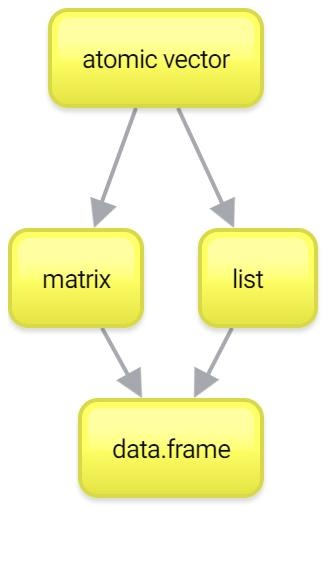
\includegraphics[width=4.16667in,height=\textheight]{images/New-Mind-Map.jpg}

\hypertarget{sec-complex_structures}{%
\chapter{Сложные структуры данных в R}\label{sec-complex_structures}}

Давайте повторим то, что мы знаем про вектор в R:

\begin{itemize}
\item
  Вектор -- это последовательность из значений.
\item
  Порядок значений имеет значение, но этот порядок одномерный.
\item
  Внутри вектора могут быть данные только одного типа
\end{itemize}

Как вы уже поняли, вектор -- это одно из важнейших понятий в R, и он нам
будет встречаться дальше постоянно. Обычно работа с данными -- это
именно работа с векторами, различные операции на векторах.

Однако иногда в понятии вектора нам уже становится несколько тесно.
Поэтому нам нужно выйти за рамки его ограничений. Во-первых, во второе
(и дальнейшие) измерения -- это делает \textbf{матрица (matrix)}.
Во-вторых, нам нужна структура, которая могла бы содержать данные разных
типов -- это \textbf{список (list).}

\hypertarget{sec-matrix}{%
\section{Матрица}\label{sec-matrix}}

Если вдруг вас пугает это слово, то совершенно зря. \textbf{Матрица
(matrix)} -- это всего лишь ``двумерный'' вектор: вектор, у которого
есть не только длина, но и ширина. Создать матрицу можно с помощью
функции \texttt{matrix()} из вектора, указав при этом количество строк и
столбцов.

\begin{Shaded}
\begin{Highlighting}[]
\NormalTok{A }\OtherTok{\textless{}{-}} \FunctionTok{matrix}\NormalTok{(}\DecValTok{1}\SpecialCharTok{:}\DecValTok{20}\NormalTok{, }\AttributeTok{nrow =} \DecValTok{5}\NormalTok{, }\AttributeTok{ncol =} \DecValTok{4}\NormalTok{)}
\NormalTok{A}
\end{Highlighting}
\end{Shaded}

\begin{verbatim}
     [,1] [,2] [,3] [,4]
[1,]    1    6   11   16
[2,]    2    7   12   17
[3,]    3    8   13   18
[4,]    4    9   14   19
[5,]    5   10   15   20
\end{verbatim}

\begin{tcolorbox}[enhanced jigsaw, leftrule=.75mm, toprule=.15mm, left=2mm, breakable, arc=.35mm, rightrule=.15mm, colback=white, opacityback=0, bottomrule=.15mm]

\textbf{\emph{Полезное:} порядок заполнения матрицы}\vspace{2mm}

Заметьте, значения вектора заполняются следующим образом: сначала
заполняется первый столбик сверху вниз, потом второй сверху вниз и так
до конца, т.е. заполнение значений матрицы идет в первую очередь по
вертикали. Это довольно стандартный способ создания матриц, характерный
не только для R.

\end{tcolorbox}

Если мы знаем сколько значений в матрице и сколько мы хотим строк, то
количество столбцов указывать необязательно:

\begin{Shaded}
\begin{Highlighting}[]
\NormalTok{A }\OtherTok{\textless{}{-}} \FunctionTok{matrix}\NormalTok{(}\DecValTok{1}\SpecialCharTok{:}\DecValTok{20}\NormalTok{, }\AttributeTok{nrow =} \DecValTok{5}\NormalTok{)}
\NormalTok{A}
\end{Highlighting}
\end{Shaded}

\begin{verbatim}
     [,1] [,2] [,3] [,4]
[1,]    1    6   11   16
[2,]    2    7   12   17
[3,]    3    8   13   18
[4,]    4    9   14   19
[5,]    5   10   15   20
\end{verbatim}

Все остальное так же как и с векторами: внутри находится данные только
одного типа. Поскольку матрица -- это уже двумерный массив, то у него
имеется два индекса. Эти два индекса разделяются запятыми.

\begin{Shaded}
\begin{Highlighting}[]
\NormalTok{A[}\DecValTok{2}\NormalTok{, }\DecValTok{3}\NormalTok{]}
\end{Highlighting}
\end{Shaded}

\begin{verbatim}
[1] 12
\end{verbatim}

Первый индекс -- выбор строк, второй индекс -- выбор колонок\footnote{Это
  универсальный порядок: что в других языках программирования, что в
  линейной алгебре первый индекс -- выбор строчек, второй индекс --
  выбор столбцов.}. Результат -- пересечение выбранных строк и столбцов.

Так же как и с векторами, матрицы можно индексировать числовыми
векторами:

\begin{Shaded}
\begin{Highlighting}[]
\NormalTok{A[}\DecValTok{2}\SpecialCharTok{:}\DecValTok{4}\NormalTok{, }\DecValTok{1}\SpecialCharTok{:}\DecValTok{3}\NormalTok{]}
\end{Highlighting}
\end{Shaded}

\begin{verbatim}
     [,1] [,2] [,3]
[1,]    2    7   12
[2,]    3    8   13
[3,]    4    9   14
\end{verbatim}

И даже логическими матрицами (матрицы имеют такие же типы, как и
вектора):

\begin{Shaded}
\begin{Highlighting}[]
\NormalTok{A[A }\SpecialCharTok{\textgreater{}} \DecValTok{10}\NormalTok{]}
\end{Highlighting}
\end{Shaded}

\begin{verbatim}
 [1] 11 12 13 14 15 16 17 18 19 20
\end{verbatim}

В этом случае матрица упростится до вектора.

Если же мы оставляем пустое поле вместо числа, то мы выбираем все
строки/колонки в зависимости от того, оставили мы поле пустым до или
после запятой:

\begin{Shaded}
\begin{Highlighting}[]
\NormalTok{A[, }\DecValTok{1}\SpecialCharTok{:}\DecValTok{3}\NormalTok{]}
\end{Highlighting}
\end{Shaded}

\begin{verbatim}
     [,1] [,2] [,3]
[1,]    1    6   11
[2,]    2    7   12
[3,]    3    8   13
[4,]    4    9   14
[5,]    5   10   15
\end{verbatim}

\begin{Shaded}
\begin{Highlighting}[]
\NormalTok{A[}\DecValTok{2}\SpecialCharTok{:}\DecValTok{4}\NormalTok{, ]}
\end{Highlighting}
\end{Shaded}

\begin{verbatim}
     [,1] [,2] [,3] [,4]
[1,]    2    7   12   17
[2,]    3    8   13   18
[3,]    4    9   14   19
\end{verbatim}

\begin{Shaded}
\begin{Highlighting}[]
\NormalTok{A[, ]}
\end{Highlighting}
\end{Shaded}

\begin{verbatim}
     [,1] [,2] [,3] [,4]
[1,]    1    6   11   16
[2,]    2    7   12   17
[3,]    3    8   13   18
[4,]    4    9   14   19
[5,]    5   10   15   20
\end{verbatim}

Так же как и в случае с обычными векторами, часть матрицы можно
переписать:

\begin{Shaded}
\begin{Highlighting}[]
\NormalTok{A[}\DecValTok{2}\SpecialCharTok{:}\DecValTok{4}\NormalTok{, }\DecValTok{2}\SpecialCharTok{:}\DecValTok{4}\NormalTok{] }\OtherTok{\textless{}{-}} \DecValTok{100}
\NormalTok{A}
\end{Highlighting}
\end{Shaded}

\begin{verbatim}
     [,1] [,2] [,3] [,4]
[1,]    1    6   11   16
[2,]    2  100  100  100
[3,]    3  100  100  100
[4,]    4  100  100  100
[5,]    5   10   15   20
\end{verbatim}

В принципе, это все, что нам нужно знать о матрицах. Матрицы
используются в R довольно редко, особенно по сравнению, например, с
MATLAB. Но вот индексировать матрицы хорошо бы уметь: это понадобится в
работе с датафреймами (см. Глава~\ref{sec-df}).

\begin{tcolorbox}[enhanced jigsaw, leftrule=.75mm, toprule=.15mm, left=2mm, breakable, arc=.35mm, rightrule=.15mm, colback=white, opacityback=0, bottomrule=.15mm]

\textbf{\emph{Для продвинутых:} матрица как вектор}\vspace{2mm}

То, что матрица -- это просто двумерный вектор, не является метафорой: в
R матрица -- это по сути своей вектор с дополнительными
\emph{атрибутами} \texttt{dim} и (опционально) \texttt{dimnames}.
Атрибуты -- это свойства объектов, своего рода ``метаданные''. Для всех
объектов есть обязательные атрибуты типа и длины и могут быть любые
необязательные атрибуты. Можно задавать свои атрибуты или удалять уже
присвоенные: удаление атрибута \texttt{dim} у матрицы превратит ее в
обычный вектор. Про атрибуты подробнее можно почитать
\href{https://perso.esiee.fr/~courivad/R/06-objects.html}{здесь} или на
стр. 99-101 книги ``R in a Nutshell'' (Adler 2010).

\end{tcolorbox}

\hypertarget{sec-arrays}{%
\section{Массив}\label{sec-arrays}}

Два измерения -- это не предел! Структура с одним типом данных внутри,
но с тремя измерениями или больше, называется \textbf{массивом (array)}.
Создание массива очень похоже на создание матрицы: задаем вектор, из
которого будет собран массив, и размерность массива.

\begin{Shaded}
\begin{Highlighting}[]
\NormalTok{array\_3d }\OtherTok{\textless{}{-}} \FunctionTok{array}\NormalTok{(}\DecValTok{1}\SpecialCharTok{:}\DecValTok{12}\NormalTok{, }\FunctionTok{c}\NormalTok{(}\DecValTok{3}\NormalTok{, }\DecValTok{2}\NormalTok{, }\DecValTok{2}\NormalTok{))}
\NormalTok{array\_3d}
\end{Highlighting}
\end{Shaded}

\begin{verbatim}
, , 1

     [,1] [,2]
[1,]    1    4
[2,]    2    5
[3,]    3    6

, , 2

     [,1] [,2]
[1,]    7   10
[2,]    8   11
[3,]    9   12
\end{verbatim}

\hypertarget{sec-list}{%
\section{Список}\label{sec-list}}

Теперь представим себе вектор без ограничения на одинаковые данные
внутри. И получим \textbf{список (list)}!

\begin{Shaded}
\begin{Highlighting}[]
\NormalTok{simple\_list }\OtherTok{\textless{}{-}} \FunctionTok{list}\NormalTok{(}\DecValTok{42}\NormalTok{, }\StringTok{"Пам пам"}\NormalTok{, }\ConstantTok{TRUE}\NormalTok{)}
\NormalTok{simple\_list}
\end{Highlighting}
\end{Shaded}

\begin{verbatim}
[[1]]
[1] 42

[[2]]
[1] "Пам пам"

[[3]]
[1] TRUE
\end{verbatim}

А это значит, что там могут содержаться самые разные данные, в том числе
и другие списки, векторы и матрицы (и другие объекты, которые нам еще не
знакомы)!

\begin{Shaded}
\begin{Highlighting}[]
\NormalTok{complex\_list }\OtherTok{\textless{}{-}} \FunctionTok{list}\NormalTok{(}\FunctionTok{c}\NormalTok{(}\StringTok{"Wow"}\NormalTok{, }\StringTok{"this"}\NormalTok{, }\StringTok{"list"}\NormalTok{, }\StringTok{"is"}\NormalTok{, }\StringTok{"so"}\NormalTok{, }\StringTok{"big"}\NormalTok{), }\StringTok{"16"}\NormalTok{, simple\_list, A)}
\NormalTok{complex\_list}
\end{Highlighting}
\end{Shaded}

\begin{verbatim}
[[1]]
[1] "Wow"  "this" "list" "is"   "so"   "big" 

[[2]]
[1] "16"

[[3]]
[[3]][[1]]
[1] 42

[[3]][[2]]
[1] "Пам пам"

[[3]][[3]]
[1] TRUE


[[4]]
     [,1] [,2] [,3] [,4]
[1,]    1    6   11   16
[2,]    2  100  100  100
[3,]    3  100  100  100
[4,]    4  100  100  100
[5,]    5   10   15   20
\end{verbatim}

Если у нас сложный список, то есть очень классная функция
\texttt{str()}, чтобы посмотреть, как он устроен:

\begin{Shaded}
\begin{Highlighting}[]
\FunctionTok{str}\NormalTok{(complex\_list)}
\end{Highlighting}
\end{Shaded}

\begin{verbatim}
List of 4
 $ : chr [1:6] "Wow" "this" "list" "is" ...
 $ : chr "16"
 $ :List of 3
  ..$ : num 42
  ..$ : chr "Пам пам"
  ..$ : logi TRUE
 $ : num [1:5, 1:4] 1 2 3 4 5 6 100 100 100 10 ...
\end{verbatim}

\begin{quote}
Представьте, что список - это такое дерево с ветвистой структурой. А на
конце этих ветвей - листья-векторы.
\end{quote}

Как и в случае с векторами мы можем давать имена элементам списка:

\begin{Shaded}
\begin{Highlighting}[]
\NormalTok{named\_list }\OtherTok{\textless{}{-}} \FunctionTok{list}\NormalTok{(}\AttributeTok{name =} \StringTok{"Veronika"}\NormalTok{, }\AttributeTok{age =} \DecValTok{26}\NormalTok{, }\AttributeTok{student =} \ConstantTok{FALSE}\NormalTok{)}
\NormalTok{named\_list}
\end{Highlighting}
\end{Shaded}

\begin{verbatim}
$name
[1] "Veronika"

$age
[1] 26

$student
[1] FALSE
\end{verbatim}

К списку можно обращаться как с помощью индексов, так и по именам.
Начнем с последнего:

\begin{Shaded}
\begin{Highlighting}[]
\NormalTok{named\_list}\SpecialCharTok{$}\NormalTok{age}
\end{Highlighting}
\end{Shaded}

\begin{verbatim}
[1] 26
\end{verbatim}

А вот с индексами сложнее, и в этом очень легко запутаться. Давайте
попробуем сделать так, как мы делали это раньше:

\begin{Shaded}
\begin{Highlighting}[]
\NormalTok{named\_list[}\DecValTok{1}\NormalTok{]}
\end{Highlighting}
\end{Shaded}

\begin{verbatim}
$name
[1] "Veronika"
\end{verbatim}

Мы, по сути, получили элемент списка -- просто как часть списка, т.е.
как список длиной один:

\begin{Shaded}
\begin{Highlighting}[]
\FunctionTok{class}\NormalTok{(named\_list)}
\end{Highlighting}
\end{Shaded}

\begin{verbatim}
[1] "list"
\end{verbatim}

\begin{Shaded}
\begin{Highlighting}[]
\FunctionTok{class}\NormalTok{(named\_list[}\DecValTok{1}\NormalTok{])}
\end{Highlighting}
\end{Shaded}

\begin{verbatim}
[1] "list"
\end{verbatim}

А вот чтобы добраться до самого элемента списка (и сделать с ним что-то
хорошее), нам нужна не одна, а две квадратных скобочки:

\begin{Shaded}
\begin{Highlighting}[]
\NormalTok{named\_list[[}\DecValTok{1}\NormalTok{]]}
\end{Highlighting}
\end{Shaded}

\begin{verbatim}
[1] "Veronika"
\end{verbatim}

\begin{Shaded}
\begin{Highlighting}[]
\FunctionTok{class}\NormalTok{(named\_list[[}\DecValTok{1}\NormalTok{]])}
\end{Highlighting}
\end{Shaded}

\begin{verbatim}
[1] "character"
\end{verbatim}

Как и в случае с вектором, к элементу списка можно обращаться по имени.
Здесь тоже будет иметь значение, одинарные или двойные квадратные скобки
вы используете:

\begin{Shaded}
\begin{Highlighting}[]
\NormalTok{named\_list[}\StringTok{"age"}\NormalTok{]}
\end{Highlighting}
\end{Shaded}

\begin{verbatim}
$age
[1] 26
\end{verbatim}

\begin{Shaded}
\begin{Highlighting}[]
\NormalTok{named\_list[[}\StringTok{"age"}\NormalTok{]]}
\end{Highlighting}
\end{Shaded}

\begin{verbatim}
[1] 26
\end{verbatim}

Хотя последнее -- практически то же самое, что и использование знака
\texttt{\$}.

\begin{tcolorbox}[enhanced jigsaw, leftrule=.75mm, toprule=.15mm, left=2mm, breakable, arc=.35mm, rightrule=.15mm, colback=white, opacityback=0, bottomrule=.15mm]

\textbf{\emph{Полезное:} зачем нужны списки}\vspace{2mm}

Списки довольно часто используются в R, но реже, чем в \emph{Python.} Со
многими объектами в R, такими как результаты статистических тестов,
удобно работать именно как со списками -- к ним все вышеописанное
применимо. Кроме того, некоторые данные мы изначально получаем в виде
древообразной структуры -- хочешь не хочешь, а придется работать с этим
как со списком. Но обычно после этого стоит как можно скорее превратить
список в датафрейм.

\end{tcolorbox}

\hypertarget{sec-df}{%
\section{Датафрейм}\label{sec-df}}

Итак, мы перешли к самому главному. Самому-самому. \textbf{Датафреймы
(dataframes)}. Более того, сейчас станет понятно, зачем нам нужно было
разбираться со всеми предыдущими темами.

Без векторов мы не смогли бы разобраться с матрицами и списками. А без
последних мы не сможем понять, что такое датафрейм.

Представьте себе, что мы хотим записать различную информацию о
нескольких респондентах. Мы могли бы записать это в список из векторов.

\begin{Shaded}
\begin{Highlighting}[]
\FunctionTok{list}\NormalTok{(}\AttributeTok{name =}  \FunctionTok{c}\NormalTok{(}\StringTok{"Veronika"}\NormalTok{, }\StringTok{"Eugeny"}\NormalTok{, }\StringTok{"Lena"}\NormalTok{, }\StringTok{"Misha"}\NormalTok{, }\StringTok{"Sasha"}\NormalTok{), }
     \AttributeTok{age =} \FunctionTok{c}\NormalTok{(}\DecValTok{26}\NormalTok{, }\DecValTok{34}\NormalTok{, }\DecValTok{23}\NormalTok{, }\DecValTok{27}\NormalTok{, }\DecValTok{26}\NormalTok{), }
     \AttributeTok{student =} \FunctionTok{c}\NormalTok{(}\ConstantTok{FALSE}\NormalTok{, }\ConstantTok{FALSE}\NormalTok{, }\ConstantTok{TRUE}\NormalTok{, }\ConstantTok{TRUE}\NormalTok{, }\ConstantTok{TRUE}\NormalTok{))}
\end{Highlighting}
\end{Shaded}

\begin{verbatim}
$name
[1] "Veronika" "Eugeny"   "Lena"     "Misha"    "Sasha"   

$age
[1] 26 34 23 27 26

$student
[1] FALSE FALSE  TRUE  TRUE  TRUE
\end{verbatim}

Датафрейм очень похож на список. Просто поменяем в команде выше list()
на data.frame() и посмотрим, что изменится:

\begin{Shaded}
\begin{Highlighting}[]
\NormalTok{df }\OtherTok{\textless{}{-}} \FunctionTok{data.frame}\NormalTok{(}\AttributeTok{name =}  \FunctionTok{c}\NormalTok{(}\StringTok{"Veronika"}\NormalTok{, }\StringTok{"Eugeny"}\NormalTok{, }\StringTok{"Lena"}\NormalTok{, }\StringTok{"Misha"}\NormalTok{, }\StringTok{"Sasha"}\NormalTok{), }
                 \AttributeTok{age =} \FunctionTok{c}\NormalTok{(}\DecValTok{26}\NormalTok{, }\DecValTok{34}\NormalTok{, }\DecValTok{23}\NormalTok{, }\DecValTok{27}\NormalTok{, }\DecValTok{26}\NormalTok{), }
                 \AttributeTok{student =} \FunctionTok{c}\NormalTok{(}\ConstantTok{FALSE}\NormalTok{, }\ConstantTok{FALSE}\NormalTok{, }\ConstantTok{TRUE}\NormalTok{, }\ConstantTok{TRUE}\NormalTok{, }\ConstantTok{TRUE}\NormalTok{))}
\FunctionTok{str}\NormalTok{(df)}
\end{Highlighting}
\end{Shaded}

\begin{verbatim}
'data.frame':   5 obs. of  3 variables:
 $ name   : chr  "Veronika" "Eugeny" "Lena" "Misha" ...
 $ age    : num  26 34 23 27 26
 $ student: logi  FALSE FALSE TRUE TRUE TRUE
\end{verbatim}

\begin{Shaded}
\begin{Highlighting}[]
\NormalTok{df}
\end{Highlighting}
\end{Shaded}

\begin{verbatim}
      name age student
1 Veronika  26   FALSE
2   Eugeny  34   FALSE
3     Lena  23    TRUE
4    Misha  27    TRUE
5    Sasha  26    TRUE
\end{verbatim}

Вообще, очень похоже на список, не правда ли? Так и есть, датафрейм --
это что-то вроде проименованного списка, каждый элемент которого
является \emph{atomic} вектором фиксированной длины. Скорее всего, вы
представляли список ``горизонтально''. Если это так, то теперь
``переверните'' список у себя в голове на 90 градусов. Так, чтобы
названия векторов оказались сверху, а элементы списка стали столбцами.

Поскольку длина всех этих векторов одинаковая (обязательное условие!),
то данные представляют собой табличку, похожую на матрицу. Но в отличие
от матрицы, разные столбцы могут иметь разные типы данных. В нашем
случае первая колонка -- \texttt{character}, вторая колонка --
\texttt{numeric}, третья колонка -- \texttt{logical}. Тем не менее,
обращаться с датафреймом можно и как с проименованным списком, и как с
матрицей:

\begin{Shaded}
\begin{Highlighting}[]
\NormalTok{df}\SpecialCharTok{$}\NormalTok{age}
\end{Highlighting}
\end{Shaded}

\begin{verbatim}
[1] 26 34 23 27 26
\end{verbatim}

Здесь мы сначала извлекли колонку \texttt{age} с помощью оператора
\texttt{\$}. Результатом этой операции является числовой вектор. Колонки
датафрейма -- это и есть векторы!

\begin{Shaded}
\begin{Highlighting}[]
\NormalTok{df}\SpecialCharTok{$}\NormalTok{age[}\DecValTok{2}\SpecialCharTok{:}\DecValTok{3}\NormalTok{]}
\end{Highlighting}
\end{Shaded}

\begin{verbatim}
[1] 34 23
\end{verbatim}

Теперь с ним можно работать как с обычным вектором: мы вытащили кусок,
выбрав индексы \texttt{2} и \texttt{3}.

Используя оператор \texttt{\$} и присваивание можно создавать новые
колонки датафрейма:

\begin{Shaded}
\begin{Highlighting}[]
\NormalTok{df}\SpecialCharTok{$}\NormalTok{lovesR }\OtherTok{\textless{}{-}} \ConstantTok{TRUE} \CommentTok{\#правило recycling {-} узнали? согласны?}
\NormalTok{df}
\end{Highlighting}
\end{Shaded}

\begin{verbatim}
      name age student lovesR
1 Veronika  26   FALSE   TRUE
2   Eugeny  34   FALSE   TRUE
3     Lena  23    TRUE   TRUE
4    Misha  27    TRUE   TRUE
5    Sasha  26    TRUE   TRUE
\end{verbatim}

Ну а можно просто обращаться с помощью двух индексов через запятую, как
мы это делали с матрицей:

\begin{Shaded}
\begin{Highlighting}[]
\NormalTok{df[}\DecValTok{3}\SpecialCharTok{:}\DecValTok{5}\NormalTok{, }\DecValTok{2}\SpecialCharTok{:}\DecValTok{3}\NormalTok{]}
\end{Highlighting}
\end{Shaded}

\begin{verbatim}
  age student
3  23    TRUE
4  27    TRUE
5  26    TRUE
\end{verbatim}

Как и с матрицами, первый индекс означает строчки, а второй -- столбцы.

А еще можно использовать названия колонок внутри квадратных скобок:

\begin{Shaded}
\begin{Highlighting}[]
\NormalTok{df[}\DecValTok{1}\SpecialCharTok{:}\DecValTok{2}\NormalTok{, }\StringTok{"age"}\NormalTok{]}
\end{Highlighting}
\end{Shaded}

\begin{verbatim}
[1] 26 34
\end{verbatim}

\begin{Shaded}
\begin{Highlighting}[]
\NormalTok{df[}\DecValTok{1}\SpecialCharTok{:}\DecValTok{2}\NormalTok{, }\FunctionTok{c}\NormalTok{(}\StringTok{"age"}\NormalTok{, }\StringTok{"name"}\NormalTok{)]}
\end{Highlighting}
\end{Shaded}

\begin{verbatim}
  age     name
1  26 Veronika
2  34   Eugeny
\end{verbatim}

И здесь перед нами открываются невообразимые возможности! Узнаем, любят
ли R те, кто моложе среднего возраста в группе:

\begin{Shaded}
\begin{Highlighting}[]
\NormalTok{df[df}\SpecialCharTok{$}\NormalTok{age }\SpecialCharTok{\textless{}} \FunctionTok{mean}\NormalTok{(df}\SpecialCharTok{$}\NormalTok{age), }\DecValTok{4}\NormalTok{]}
\end{Highlighting}
\end{Shaded}

\begin{verbatim}
[1] TRUE TRUE TRUE TRUE
\end{verbatim}

Обратите внимание, как удобно нам здесь пригодилось то, что мы научились
делать с векторами (Глава~\ref{sec-vector}). Сначала мы посчитали
среднее значение абсолютно так же, как мы делали это с векторами:

\begin{Shaded}
\begin{Highlighting}[]
\FunctionTok{mean}\NormalTok{(df}\SpecialCharTok{$}\NormalTok{age)}
\end{Highlighting}
\end{Shaded}

\begin{verbatim}
[1] 27.2
\end{verbatim}

Полученное среднее поэлементно сравнили с каждым значением колонки (т.е.
вектора) \texttt{df\$age}:

\begin{Shaded}
\begin{Highlighting}[]
\NormalTok{df}\SpecialCharTok{$}\NormalTok{age }\SpecialCharTok{\textless{}} \FunctionTok{mean}\NormalTok{(df}\SpecialCharTok{$}\NormalTok{age)}
\end{Highlighting}
\end{Shaded}

\begin{verbatim}
[1]  TRUE FALSE  TRUE  TRUE  TRUE
\end{verbatim}

Мы получили логический вектор, длина которого совпадает с длиной
датафрейма. При этом \texttt{TRUE} стоит на тех позициях, где в
соответствующей строчке в датафрейме возраст респондента больше
среднего, а \texttt{FALSE} -- в остальных случаях. Теперь этот
логический вектор мы используем для выбора строк в исходном датафрейме:

\begin{Shaded}
\begin{Highlighting}[]
\NormalTok{df[df}\SpecialCharTok{$}\NormalTok{age }\SpecialCharTok{\textless{}} \FunctionTok{mean}\NormalTok{(df}\SpecialCharTok{$}\NormalTok{age), ]}
\end{Highlighting}
\end{Shaded}

\begin{verbatim}
      name age student lovesR
1 Veronika  26   FALSE   TRUE
3     Lena  23    TRUE   TRUE
4    Misha  27    TRUE   TRUE
5    Sasha  26    TRUE   TRUE
\end{verbatim}

Наконец, тут же мы можем вытащить нужные колонки, по номеру колонки или
ее названию:

\begin{Shaded}
\begin{Highlighting}[]
\NormalTok{df[df}\SpecialCharTok{$}\NormalTok{age }\SpecialCharTok{\textless{}} \FunctionTok{mean}\NormalTok{(df}\SpecialCharTok{$}\NormalTok{age), }\DecValTok{4}\NormalTok{]}
\end{Highlighting}
\end{Shaded}

\begin{verbatim}
[1] TRUE TRUE TRUE TRUE
\end{verbatim}

Эту же задачу можно выполнить другими способами:

\begin{Shaded}
\begin{Highlighting}[]
\NormalTok{df}\SpecialCharTok{$}\NormalTok{lovesR[df}\SpecialCharTok{$}\NormalTok{age }\SpecialCharTok{\textless{}} \FunctionTok{mean}\NormalTok{(df}\SpecialCharTok{$}\NormalTok{age)]}
\end{Highlighting}
\end{Shaded}

\begin{verbatim}
[1] TRUE TRUE TRUE TRUE
\end{verbatim}

\begin{Shaded}
\begin{Highlighting}[]
\NormalTok{df[df}\SpecialCharTok{$}\NormalTok{age }\SpecialCharTok{\textless{}} \FunctionTok{mean}\NormalTok{(df}\SpecialCharTok{$}\NormalTok{age), }\StringTok{\textquotesingle{}lovesR\textquotesingle{}}\NormalTok{]}
\end{Highlighting}
\end{Shaded}

\begin{verbatim}
[1] TRUE TRUE TRUE TRUE
\end{verbatim}

В большинстве случаев подходят сразу несколько способов -- тем не менее,
стоит овладеть ими всеми. Чем богаче ваш арсенал инструментов работы в
R, тем легче вам обрабатывать свои данные: возможность сделать одно и то
же действие добавляет вам гибкости, потому что разные способы будут
более или менее подходящими в разных ситуациях.

Датафреймы удобно просматривать в RStudio. Для это нужно написать
команду \texttt{View(df)} или же просто нажать на названии нужной
переменной из списка вверху справа (там где Environment). Тогда увидите
табличку, очень похожую на Excel и тому подобные программы для работы с
таблицами. Там же есть и всякие возможности для фильтрации, сортировки и
поиска \footnote{Все, что вы нажмете в этом окошке, никак не повлияет на
  исходную переменную. Так что можете смело использовать эти функции для
  исследования содержимого датафрейма.}.

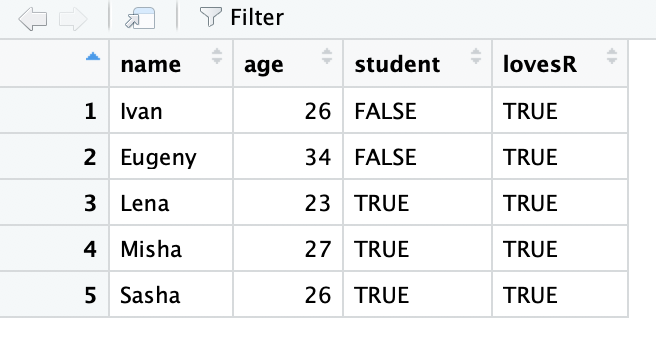
\includegraphics[width=2.08333in,height=\textheight]{images/View.png}

Но, конечно, интереснее все эти вещи делать руками, т.е. с помощью
написания кода.

Датафреймы -- это структура, которая будет встречаться вам чаще всего
при работе с данными в R. С одной стороны, кажется, что она все равно
довольно ограниченная: в каждой колонке должно быть одинаковое
количество значений, внутри колонки только один тип данных. Но именно
так обычно и представлены наши данные. Например, если вы загрузите
результаты опроса Google Forms в виде таблицы, то каждая строчка будет
респондентом, а каждая колонка -- ответом на какой-то вопрос. Поэтому
количество значений в каждой колонке будет одинаковым (хотя значения
могут быть пропущенными), а каждая колонка -- имеет свой тип. Например,
год рождения -- и это должна быть числовая колонка, с которой вы сможете
делать все, что вы умеете делать с числовыми колонками. Например,
посчитать возраст. Если в колонке с годом рождения оказалось что-то
кроме чисел, то это повод для исследования данных.

\hypertarget{sec-attr_class}{%
\section{Атрибуты и классы}\label{sec-attr_class}}

\ldots{}

\hypertarget{sec-formula}{%
\section{Формулы}\label{sec-formula}}

Формулы -- это специальный класс в R, который используется в первую
очередь для статистических моделей.

Выглядит формула следующим образом:

\begin{Shaded}
\begin{Highlighting}[]
\NormalTok{y }\SpecialCharTok{\textasciitilde{}}\NormalTok{ x}
\end{Highlighting}
\end{Shaded}

\begin{verbatim}
y ~ x
\end{verbatim}

\begin{Shaded}
\begin{Highlighting}[]
\FunctionTok{class}\NormalTok{(y }\SpecialCharTok{\textasciitilde{}}\NormalTok{ x)}
\end{Highlighting}
\end{Shaded}

\begin{verbatim}
[1] "formula"
\end{verbatim}

Как видите, здесь нет никаких кавычек, т.е. это не строковое значение, а
отдельный класс. В каждой формуле должна быть тильда
(\texttt{\textasciitilde{}}), которая имеет смысл знака равно (=) в
уравнениях (например, для уравнений линейной регрессии). Слева от
\texttt{\textasciitilde{}} обычно находится зависимая переменная, а
справа -- независимые (предикторы).

Кроме статистических моделей, формулы используются много где как
служебная конструкция, чтобы задать соответствующие пары значений. Вот
несколько примеров:

\begin{itemize}
\tightlist
\item
  \texttt{case\_when()} для задания множественных условий (см.
  Глава~\ref{sec-ifelse}),
\item
  визуализация ящиков с усами в базовом R (см. Глава~\ref{sec-r_vis}),
\item
  статистические тесты для сравнения двух (см. Глава~\ref{sec-ttest}) и
  более (см. Глава~\ref{sec-anova}) групп,
\item
  задание фасеток в \{ggplot2\} (см. Глава~\ref{sec-gg_ggplot2}).
\end{itemize}

\hypertarget{sec-r_packages}{%
\chapter{Пакеты в R}\label{sec-r_packages}}

\hypertarget{sec-extra_pack}{%
\section{Дополнительные пакеты}\label{sec-extra_pack}}

R --- очень богатый язык с широкими возможностями. Однако очень скоро мы
поймем, что этих возможностей нам не хватает. Эти возможности нам могут
предоставить дополнительные \textbf{пакеты (packages)}.

В большинстве случаев основным содержанием пакетов является набор
дополнительных функций. Кроме функций, пакеты могут содержать наборы
данных и новые структуры данных.

Обычно пакеты посвящены решению какого-то класса задач в определенной
области. Например, есть множество пакетов для создания какого-то одного
типа визуализации. Еще один пример --- пакет \texttt{beepr}, который
содержит всего две функции: \texttt{beep()} и \texttt{beep\_on\_error()}
для воспроизведения звукового сигнала. Это может быть удобно, если ваш
скрипт работает долго, но вы хотите получить уведомление, когда его
выполнение завершится.

Более крупные пакеты посвящены целому классу задач. Например, пакеты
\texttt{stringi} и \texttt{stringr} посвящены работе со строками,
значительно расширяя и делая более удобной работу со строковыми данными
в R. Еще один пример: пакет \texttt{igraph} для работы с графами
(сетями). Этот пакет предоставляет дополнительный класс данных
\texttt{igraph} для хранения и работы с сетями.

Есть и совсем крупные пакеты, которые значительно расширяют базовый
функционал R, изменяя основные принципы работы в нем. Это пакеты
\texttt{data.table} и \texttt{tidyverse}. Это настолько крупные пакеты,
что их даже называют отдельными диалектами R, потому что код, написанный
с использованием этих пакетов, довольно сильно отличается от базового R.
Кроме того, \emph{tidyverse} - это не просто пакет, а целая экосистема
пакетов, который взаимодополняют друг друга, но для удобства их можно
устанавливать и загружать как один пакет \texttt{tidyverse}. Еще один
пример крупной экосистемы из пакетов --- это пакеты \texttt{mlr3} и
\texttt{tidymodels} для машинного обучения, который представляет собой
большой расширяемый ``пакет пакетов'', где отдельные пакеты посвящены
отдельным этапам и задачам машинного обучения.

\hypertarget{sec-r_built_in}{%
\section{Встроенные пакеты R}\label{sec-r_built_in}}

Вообще, даже сам R является набором из нескольких пакетов: основного
\texttt{base} и нескольких других, таких как \texttt{stats},
\texttt{utils}, \texttt{graphics}. Вот их полный список:

\begin{Shaded}
\begin{Highlighting}[]
\FunctionTok{rownames}\NormalTok{(}\FunctionTok{installed.packages}\NormalTok{(}\AttributeTok{priority =} \StringTok{"base"}\NormalTok{))}
\end{Highlighting}
\end{Shaded}

\begin{verbatim}
 [1] "base"      "compiler"  "datasets"  "graphics"  "grDevices" "grid"     
 [7] "methods"   "parallel"  "splines"   "stats"     "stats4"    "tcltk"    
[13] "tools"     "utils"    
\end{verbatim}

Чтобы пользоваться этими пакетами ничего дополнительно делать не нужно.

\hypertarget{sec-install_cran}{%
\section{Установка пакетов с CRAN}\label{sec-install_cran}}

Функция \texttt{install.packages()} позволяет скачивать пакеты с
\href{https://cran.r-project.org}{Comprehensive R Archive Network
(CRAN)}. На репозитории \emph{CRAN} собрано более 19000 пакетов (число
постоянно меняется, как в большую, так и меньшую сторону). Каждый из
этих пакетов проходит проверку перед попаданием в \emph{CRAN}: он должен
быть хорошо задокументирован, стабильно работать и решать какую-то
задачу.

Для примера установим пакет \texttt{remotes}. Это пакет для удобной
установки пакетов не с \emph{CRAN} и скоро нам понадобится.

\begin{Shaded}
\begin{Highlighting}[]
\FunctionTok{install.packages}\NormalTok{(}\StringTok{"remotes"}\NormalTok{)}
\end{Highlighting}
\end{Shaded}

При установке вы увидите много непонятных надписей красным (или черным)
шрифтом. Не пугайтесь, это нормально, происходит скачивание и установка
пакетов. Скорее всего, если нигде нет слова \emph{Error}, то пакет
успешно установился.

Иногда установка бывает очень долгой, потому что большие пакеты склонны
иметь много \textbf{зависимостей}: для работы какого-то пакета может
понадобиться другие пакеты, а для тех пакетов - еще какие-то пакеты.
Таким образом, устанавливая какой-нибудь современный пакет, вы,
возможно, установите десятки других пакетов! Зато если они понадобятся
сами по себе, то их уже не нужно будет устанавливать.

\hypertarget{sec-package_load}{%
\section{Загрузка установленного пакета}\label{sec-package_load}}

Установить пакет с помощью \texttt{install.packages()} недостаточно,
пакет нужно еще загрузить. Для этого есть функция \texttt{library()}.

\begin{Shaded}
\begin{Highlighting}[]
\FunctionTok{library}\NormalTok{(}\StringTok{"remotes"}\NormalTok{)}
\end{Highlighting}
\end{Shaded}

В отличие от \texttt{install.packages()}, функция \texttt{library()}
принимает название пакета и как строчку в кавычках, и как название без
кавычек.

\begin{Shaded}
\begin{Highlighting}[]
\FunctionTok{library}\NormalTok{(remotes)}
\end{Highlighting}
\end{Shaded}

Теперь функции, данные и классы из пакета доступны для работы.

\begin{tcolorbox}[enhanced jigsaw, leftrule=.75mm, toprule=.15mm, left=2mm, breakable, arc=.35mm, rightrule=.15mm, colback=white, opacityback=0, bottomrule=.15mm]

\textbf{\emph{Полезное:} аналогия с \emph{Python}}\vspace{2mm}

Если сравнивать с \emph{Python}, то \texttt{install.packages()} -- это
аналог установки библиотек, например, с помощью \emph{pip}, а
\texttt{library()} -- это аналог \texttt{import} (например,
\texttt{import\ pandas\ as\ pd}).

\end{tcolorbox}

\hypertarget{sec-from_package}{%
\section{\texorpdfstring{Вызов функции из пакета с помощью
\texttt{::}}{Вызов функции из пакета с помощью ::}}\label{sec-from_package}}

Если пакетом нужно воспользоваться всего один-два раза, то имеет смысл
не подключать весь пакет, а загрузить отдельную функцию из него. Для
этого есть специальный оператор \texttt{::}, который использует функцию
(указанную справа от \texttt{::}) из выбранного пакета (указанного слева
от \texttt{::}), не загружая пакет полностью.

Для примера воспользуемся функцией \texttt{package\_deps()} из только
что установленного пакета \texttt{remotes}, которая возвращает все
зависимости пакета:

\begin{Shaded}
\begin{Highlighting}[]
\NormalTok{remotes}\SpecialCharTok{::}\FunctionTok{package\_deps}\NormalTok{(}\StringTok{"tidyverse"}\NormalTok{)}
\end{Highlighting}
\end{Shaded}

\begin{verbatim}
Needs update -----------------------------
 package      installed available is_cran remote
 cpp11        0.4.3     0.4.4     TRUE    CRAN  
 vctrs        0.6.2     0.6.3     TRUE    CRAN  
 sys          3.4.1     3.4.2     TRUE    CRAN  
 jsonlite     1.8.5     1.8.7     TRUE    CRAN  
 curl         5.0.0     5.0.1     TRUE    CRAN  
 xml2         1.3.3     1.3.4     TRUE    CRAN  
 httr         1.4.5     1.4.6     TRUE    CRAN  
 fastmap      1.1.0     1.1.1     TRUE    CRAN  
 digest       0.6.31    0.6.32    TRUE    CRAN  
 sass         0.4.5     0.4.6     TRUE    CRAN  
 cachem       1.0.6     1.0.8     TRUE    CRAN  
 tinytex      0.44      0.45      TRUE    CRAN  
 htmltools    0.5.4     0.5.5     TRUE    CRAN  
 fontawesome  0.5.0     0.5.1     TRUE    CRAN  
 bslib        0.4.2     0.5.0     TRUE    CRAN  
 xfun         0.37      0.39      TRUE    CRAN  
 processx     3.8.1     3.8.2     TRUE    CRAN  
 rmarkdown    2.20      2.23      TRUE    CRAN  
 knitr        1.42      1.43      TRUE    CRAN  
 tzdb         0.3.0     0.4.0     TRUE    CRAN  
 vroom        1.6.1     1.6.3     TRUE    CRAN  
 broom        1.0.4     1.0.5     TRUE    CRAN  
 readr        2.1.3     2.1.4     TRUE    CRAN  
 googledrive  2.0.0     2.1.1     TRUE    CRAN  
 gargle       1.3.0     1.5.1     TRUE    CRAN  
 blob         1.2.3     1.2.4     TRUE    CRAN  
 modelr       0.1.10    0.1.11    TRUE    CRAN  
 lubridate    1.9.1     1.9.2     TRUE    CRAN  
 haven        2.5.1     2.5.3     TRUE    CRAN  
 googleshe... 1.0.1     1.1.1     TRUE    CRAN  
 dtplyr       1.2.2     1.3.1     TRUE    CRAN  
 dbplyr       2.3.0     2.3.2     TRUE    CRAN  
 conflicted   NA        1.2.0     TRUE    CRAN  
 tidyverse    1.3.2     2.0.0     TRUE    CRAN  
\end{verbatim}

В дальнейшем использование оператора \texttt{::} будет иногда
использоваться, чтобы указать, из какого пакета взята функция.

Оператор \texttt{::} полезен еще и в тех случаях, когда в разных пакетах
присутствуют функции с одинаковым названием. Например, у основного
пакета tidyverse, \texttt{dplyr}, есть функция \texttt{filter()}.
Функция с точно таким же названием есть в базовом R в пакете
\texttt{stats}, в котором та выполняет совершенно другую задачу. Если у
вас уже загружен \texttt{dplyr}, то использование \texttt{::} укажет на
то, что вы хотите воспользоваться именно функцией \texttt{filter()} из
пакета \texttt{stats}:

\begin{Shaded}
\begin{Highlighting}[]
\NormalTok{stats}\SpecialCharTok{::}\FunctionTok{filter}\NormalTok{(}\DecValTok{1}\SpecialCharTok{:}\DecValTok{20}\NormalTok{, }\FunctionTok{rep}\NormalTok{(}\DecValTok{1}\NormalTok{,}\DecValTok{3}\NormalTok{))}
\end{Highlighting}
\end{Shaded}

\begin{verbatim}
Time Series:
Start = 1 
End = 20 
Frequency = 1 
 [1] NA  6  9 12 15 18 21 24 27 30 33 36 39 42 45 48 51 54 57 NA
\end{verbatim}

Подобные путаницы могут возникнуть, если у вас загружено много пакетов,
поэтому старайтесь не загружать слишком много пакетов, а если есть
функции с одинаковым названием, то обязательно используйте оператор
\texttt{::}. Иначе слишком велик риск загрузить пакеты не в том порядке
и получить из-за этого ошибку или некорректный результат.

\begin{tcolorbox}[enhanced jigsaw, leftrule=.75mm, toprule=.15mm, left=2mm, breakable, arc=.35mm, rightrule=.15mm, colback=white, opacityback=0, bottomrule=.15mm]

\textbf{\emph{Полезное:} оператор \texttt{::} для указания используемого
пакета}\vspace{2mm}

В дальнейшем я буду иногда использовать \texttt{::}, чтобы было понятно,
из какого пакета взята та или иная функция

\end{tcolorbox}

Выгрузить ненужный пакет можно с помощью функции \texttt{detach()}.

\begin{Shaded}
\begin{Highlighting}[]
\FunctionTok{detach}\NormalTok{(package}\SpecialCharTok{:}\NormalTok{remotes)}
\end{Highlighting}
\end{Shaded}

\hypertarget{sec-install_bioc}{%
\section{Установка пакетов c Bioconductor}\label{sec-install_bioc}}

У биологов есть свой большой репозиторий, который является альтернативой
\emph{CRAN}, --- \emph{Bioconductor}. С него можно скачать множество
специализированных пакетов для работы с биологическими данными.

Для установки пакетов с Bioconductor сначала нужно скачать пакет
\texttt{BiocManager} с CRAN.

\begin{Shaded}
\begin{Highlighting}[]
\FunctionTok{install.packages}\NormalTok{(}\StringTok{"BiocManager"}\NormalTok{)}
\end{Highlighting}
\end{Shaded}

Теперь можно воспользоваться функцией \texttt{install()} из пакета
\texttt{BiocManager} для установки пакета \texttt{flowCore} --- пакета
для анализа данных проточной цитометрии.

\begin{Shaded}
\begin{Highlighting}[]
\NormalTok{BiocManager}\SpecialCharTok{::}\FunctionTok{install}\NormalTok{(}\StringTok{"flowCore"}\NormalTok{)}
\end{Highlighting}
\end{Shaded}

\hypertarget{sec-install_github}{%
\section{Установка пакетов с Github}\label{sec-install_github}}

Некоторых пакетов нет ни на \emph{CRAN,} ни на \emph{Bioconductor.}
Обычно это касается пакетов, разработчики которых по каким-либо причинам
решили не проходить проверки или не прошли проверки на строгие
требования \emph{CRAN.} Иногда бывает, что пакет был удален с
\emph{CRAN} (например, автор давно не занимается им) или же версия
пакета на \emph{CRAN} отстает от последней, а именно в ней реализованы
так нужные вам функции. В некоторых случаях пакета может не быть на
\emph{CRAN}, потому что его разработчики активно занимаются его
развитием и постоянно переделывают уже имеющийся функционал, добавляя
новые возможности и удаляя старые. Это нужно делать с осторожностью,
когда пакет уже выложен на \emph{CRAN,} потому что если функции новой
версии пакета будут работать по-другому, то это может вызвать массу
проблем.

Во всех этих случаях пакет обычно можно скачать с репозитория
\emph{Github.} Для этого нам понадобится уже установленный (с
\emph{CRAN,} разумеется) пакет \texttt{remotes}\footnote{пакет
  \texttt{remotes} ``откололся'' от более старого пакета
  \texttt{devtools}, а многие функции из \texttt{remote} просто
  скопированы из \texttt{devtools}. Разработчики
  \texttt{devtools}/\texttt{remotes} рекомендуют использовать для
  установки пакетов именно более легковесный \texttt{remotes}, но во
  многих случаях вы увидите код с \texttt{devtools::install\_github()}.
  Оба варианта будут работать.}.

\begin{Shaded}
\begin{Highlighting}[]
\NormalTok{remotes}\SpecialCharTok{::}\FunctionTok{install\_github}\NormalTok{(}\StringTok{"dracor{-}org/rdracor"}\NormalTok{)}
\end{Highlighting}
\end{Shaded}

Теперь установленный пакет осталось загрузить, после чего им можно
пользоваться.

\begin{Shaded}
\begin{Highlighting}[]
\FunctionTok{library}\NormalTok{(rdracor)}
\NormalTok{godunov }\OtherTok{\textless{}{-}} \FunctionTok{get\_net\_cooccur\_igraph}\NormalTok{(}\AttributeTok{corpus =} \StringTok{"rus"}\NormalTok{,}
                                  \AttributeTok{play =} \StringTok{"pushkin{-}boris{-}godunov"}\NormalTok{)}
\FunctionTok{plot}\NormalTok{(godunov)}
\end{Highlighting}
\end{Shaded}

\begin{figure}[H]

{\centering 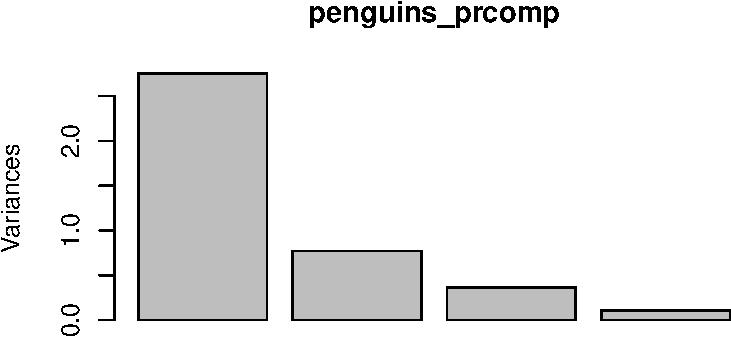
\includegraphics{020-install_files/figure-pdf/unnamed-chunk-12-1.pdf}

}

\end{figure}

Пакет \texttt{remotes} можно так же использовать для загрузки пакетов из
Bioconductor:

\begin{Shaded}
\begin{Highlighting}[]
\NormalTok{remotes}\SpecialCharTok{::}\FunctionTok{install\_bioc}\NormalTok{(}\StringTok{"flowCore"}\NormalTok{)}
\end{Highlighting}
\end{Shaded}

\hypertarget{sec-where_packages}{%
\section{Где искать нужные пакеты}\label{sec-where_packages}}

Мы разобрались с тем, как устанавливать пакеты. А где же их находить?

Это вопрос гораздо более сложный чем может показаться. Например, можно
работать в R и не знать, что существует пакет, который решает нужную для
вас задачу. Или же найти такой пакет и не знать, что есть более
современный пакет, который делает это еще лучше!

Здесь нет каких-то готовых решений. \emph{CRAN} пытается создавать и
поддерживать тематические списки \emph{(Task View)} пакетов с описанием
задач, которые они решают:

\url{https://cran.r-project.org/web/views/}

Безусловно, если вы глубоко занимаетесь какой-либо темой из списка, то
стоит изучить соотвестствующий \emph{Task View}, но начинать знакомство
с помощью \emph{Task View} достаточно тяжело.

Другой вариант --- просто погуглить, найти релевантные статьи или книги.
Внимательно смотрите на дату публикации: R --- очень быстро
развивающийся язык, поэтому с большой вероятностью то, что было написано
пять лет назад уже потеряло актуальность. Нет, работать это будет, но,
скорее всего, появился более удобный и продвинутый инструмент.

\hypertarget{sec-real_data}{%
\chapter{Импорт и экспорт данных}\label{sec-real_data}}

Итак, пришло время перейти к реальным данным. Мы начнем с использования
датасета (так мы будем называть любой набор данных) по супергероям. Этот
датасет представляет собой табличку, каждая строка которой - отдельный
супергерой, а столбик --- какая-либо информация о нем. Например, цвет
глаз, цвет волос, вселенная супергероя\footnote{супергерои в комиксах,
  фильмах и телесериалах часто взаимодействуют друг с другом, однако
  обычно это взаимодействие происходит между супергероями одного
  издателя. Два крупнейших издателя комиксов --- DC и Marvel, поэтому
  принято говорить о вселенной DC и Marvel.}, рост, вес, пол и так
далее. Несложно заметить, что этот датасет идеально подходит под
структуру датафрейма: прямоугольная табличка, внутри которой есть разные
колонки, каждая из которой имеет свой тип (числовой или строковый).

\hypertarget{sec-wd}{%
\section{Рабочая папка и проекты RStudio}\label{sec-wd}}

Для начала скачайте файл по
\href{https://raw.githubusercontent.com/Pozdniakov/tidy_stats/master/data/heroes_information.csv}{ссылке}

Он, скорее всего, появился у вас в папке ``Загрузки''. Если мы будем
просто пытаться прочитать этот файл (например, с помощью
\texttt{read.csv()} --- мы к этой функцией очень скоро перейдем), указав
его имя и разрешение, то наткнемся на такую ошибку:

\begin{Shaded}
\begin{Highlighting}[]
\FunctionTok{read.csv}\NormalTok{(}\StringTok{"heroes\_information.csv"}\NormalTok{)}
\end{Highlighting}
\end{Shaded}

\begin{verbatim}
Warning in file(file, "rt"): cannot open file 'heroes_information.csv': No such
file or directory
\end{verbatim}

\begin{verbatim}
Error in file(file, "rt"): cannot open the connection
\end{verbatim}

Это означает, что R не может найти нужный файл. Вообще-то мы даже не
сказали, где искать. Нам нужно как-то совместить место, где R ищет
загружаемые файлы и сами файлы. Для этого есть несколько способов.

\begin{itemize}
\tightlist
\item
  Магомет идет к горе: перемещение файлов в рабочую папку.
\end{itemize}

Для этого нужно узнать, какая папка является рабочей с помощью функции
\texttt{getwd()} (без аргументов), найти эту папку в проводнике и
переместить туда файл. После этого можно использовать просто название
файла с разрешением:

\begin{Shaded}
\begin{Highlighting}[]
\NormalTok{heroes }\OtherTok{\textless{}{-}} \FunctionTok{read.csv}\NormalTok{(}\StringTok{"heroes\_information.csv"}\NormalTok{)}
\end{Highlighting}
\end{Shaded}

Кроме того, путь к рабочей папке можно увидеть в RStudio во вкладке с
консолью, в самой верхней части (прямо под надписью ``Console''):


\includegraphics[width=4.16667in,height=\textheight]{images/Console_wd.png}

\begin{itemize}
\tightlist
\item
  Гора идет к Магомету: изменение рабочей папки.
\end{itemize}

Можно просто сменить рабочую папку с помощью \texttt{setwd()} на ту, где
сейчас лежит файл, прописав путь до этой папки. Теперь файл находится в
рабочей папке:

\begin{Shaded}
\begin{Highlighting}[]
\NormalTok{heroes }\OtherTok{\textless{}{-}} \FunctionTok{read.csv}\NormalTok{(}\StringTok{"heroes\_information.csv"}\NormalTok{)}
\end{Highlighting}
\end{Shaded}

Этот вариант использовать
\href{https://www.tidyverse.org/blog/2017/12/workflow-vs-script/}{не
рекомендуется}! Как минимум, это сразу делает невозможным запустить
скрипт на другом компьютере. Ну а если все-таки вдруг повезет и
получится, то ваш коллега будет очень недоволен, что ваш скрипт изменяет
рабочую директорию.

\begin{itemize}
\tightlist
\item
  Гора находит Магомета по месту прописки: указание полного пути файла.
\end{itemize}

\begin{Shaded}
\begin{Highlighting}[]
\NormalTok{heroes }\OtherTok{\textless{}{-}} \FunctionTok{read.csv}\NormalTok{(}\StringTok{"/Users/Username/Some\_Folder/heroes\_information.csv"}\NormalTok{)}
\end{Highlighting}
\end{Shaded}

Этот вариант страдает теми же проблемами, что и предыдущий, поэтому тоже
не рекомендуется!

\begin{quote}
Для пользователей Windows есть дополнительная сложность: знак \texttt{/}
является особым знаком для R, поэтому вместо него нужно использовать
двойной \texttt{//}.
\end{quote}

\begin{itemize}
\tightlist
\item
  Магомет использует кнопочный интерфейс: Import Dataset.
\end{itemize}

Во вкладке Environment справа в окне RStudio есть кнопка ``Import
Dataset''. Возможно, у Вас возникло непреодолимое желание отдохнуть от
написания кода и понажимать кнопочки --- сопротивляйтесь этому всеми
силами, но не вините себя, если не сдержитесь.

\begin{itemize}
\tightlist
\item
  Гора находит Магомета в интернете.
\end{itemize}

Многие функции в R, предназначенные для чтения файлов, могут прочитать
файл не только на Вашем компьютере, но и сразу из интернета. Для этого
просто используйте ссылку вместо пути:

\begin{Shaded}
\begin{Highlighting}[]
\NormalTok{heroes }\OtherTok{\textless{}{-}} \FunctionTok{read.csv}\NormalTok{(}\StringTok{"https://raw.githubusercontent.com/Pozdniakov/tidy\_stats/master/data/heroes\_information.csv"}\NormalTok{)}
\end{Highlighting}
\end{Shaded}

\begin{itemize}
\tightlist
\item
  Каждый Магомет получает по своей горе: использование проектов в
  RStudio.
\end{itemize}

На первый взгляд это кажется чем-то очень сложным, но это не так. Это
очень просто и ОЧЕНЬ удобно. При создании проекта создается отдельная
папка, где у вас лежат данные, хранятся скрипты, вспомогательные файлы и
отчеты. Кроме папки создается файл формата \emph{.Rproj}, в котором
хранятся настройки проекта. Если нужно вернуться к другому проекту ---
просто открываете другой проект, с другими файлами и скриптами. Можно
даже иметь открытыми несколько окон \emph{RStudio} таким образом. Это
еще помогает не пересекаться переменным из разных проектов --- а то,
знаете, использование двух переменных \texttt{data} в разных скриптах
чревато ошибками. Поэтому очень удобным решением будет выделение
отдельного проекта под этот курс.

\begin{quote}
При закрытии проекта все переменные по умолчанию тоже будут сохраняться,
а при открытии --- восстанавливаться (а вот пакеты все равно придется
подгружать заново). Это очень удобно, хотя некоторые
\href{https://r4ds.had.co.nz/workflow-projects.html}{рекомендуют от
этого отказаться}. Это можно сделать во вкладке
\texttt{Tool\ -\ Global\ Options...}
\end{quote}

\hypertarget{sec-project_workflow}{%
\section{Организация проектов}\label{sec-project_workflow}}

Даже если не пользоваться проектами RStudio (но я настоятельно
рекомендую, это очень удобно), то все равно имеет смысл разделять
различные свои проекты по отдельным папкам. Для небольших проектов этого
уже может быть достаточно, но я рекомендую делать немного более сложную
структуру папок внутри проекта. Например, такую:

\begin{verbatim}
.
└── my_project 
    ├── R 
    ├── data
    │   ├── raw
    │   ├── temp
    │   └── processed
    ├── figures
    ├── main_script.R 
    ├── my_project.Rproj
    ├── output
    └── README.txt
\end{verbatim}

В основной папке содержится автоматически созданный RStudio файл .Rproj,
основной скрипт с формат .R (или же это может быть .Rmd файл --- см.
@ref(rmd)). Вспомогательные скрипты (например, с функциями) могут
храниться в папке R. Если скриптов несколько, то их порядок стоит
обозначить числами:

\begin{verbatim}
.
├── 01_first_script_preposcessing.R
├── 02_second_script_statistics.R
└── 03_third_script_figures.R 
\end{verbatim}

Данные стоит держать в отдельной папке, причем в некоторых ситуациях вы
захотите создать отдельные подпапки, например, отдельные подпапки для
данных на входе, временных файлов и данных на выходе. Результаты работы,
например, отчеты, сгенерированные с помощью \emph{R Markdown} или
\emph{Quarto} (см. Глава~\ref{sec-rmd}). Туда же можно поместить папку с
графиками или же можно поместить эту папку в корневую директорию.

Это лишь пример структуры организации проектов, детали могут
различаться, но такая структура позволит не заблудиться в собственных
файлах, если тех накопилось достаточно много. Кроме того, другому
человеку в такой структуре проекта будет разобраться значительно проще

При создании папок внутри основного проекта важно помнить о том, что
теперь ваши файлы больше нельзя найти в вашей корневой директории: нужно
искать их в соответствующих папках. Это значит, что путь до файла теперь
будет не \texttt{"heroes\_information.csv"}, а
\texttt{"data/heroes\_information.csv"} или даже
\texttt{"data/raw/heroes\_information.csv"}.

\begin{tcolorbox}[enhanced jigsaw, leftrule=.75mm, toprule=.15mm, left=2mm, breakable, arc=.35mm, rightrule=.15mm, colback=white, opacityback=0, bottomrule=.15mm]

\textbf{\emph{Полезное:} пакет \texttt{\{here\}}}\vspace{2mm}

Пакет \texttt{\{here\}} позволяет удобно работать с путями на любых
операционных системах, создавая путь в зависимости от вашей корневой
директории проекта.

\begin{Shaded}
\begin{Highlighting}[]
\NormalTok{here}\SpecialCharTok{::}\FunctionTok{here}\NormalTok{(}\StringTok{"data"}\NormalTok{, }\StringTok{"heroes\_information.csv"}\NormalTok{)}
\end{Highlighting}
\end{Shaded}

\begin{verbatim}
[1] "/Users/ivan/R/tidy_stats/data/heroes_information.csv"
\end{verbatim}

Созданный путь можно использовать для чтения файлов:

\begin{Shaded}
\begin{Highlighting}[]
\NormalTok{heroes }\OtherTok{\textless{}{-}} \FunctionTok{read.csv}\NormalTok{(here}\SpecialCharTok{::}\FunctionTok{here}\NormalTok{(}\StringTok{"data"}\NormalTok{, }\StringTok{"heroes\_information.csv"}\NormalTok{))}
\end{Highlighting}
\end{Shaded}

\end{tcolorbox}

Сами скрипты тоже лучше разделять на смысловые части. Для этого есть
горячие клавиши Cmd + Shift + R. Это сочетание клавиш выведет окно, в
котором вам нужно вписать название, после чего появится вот такой
аккуратный комментарий:

\begin{Shaded}
\begin{Highlighting}[]
\CommentTok{\# Meaningful part of the script {-}{-}{-}{-}{-}{-}{-}{-}{-}{-}{-}{-}{-}{-}{-}{-}{-}{-}{-}{-}{-}{-}{-}{-}{-}{-}{-}{-}{-}{-}{-}{-}{-}{-}{-}{-}{-}{-}{-}{-}{-}{-}{-}}
\end{Highlighting}
\end{Shaded}

Разделенный на такие части скрипт (да еще и с подробными комментариями)
гораздо удобнее читать!

\hypertarget{sec-text_binary}{%
\subsection{Табличные данные: текстовые и бинарные
данные}\label{sec-text_binary}}

Как вы уже поняли, импорт данных - одна из самых муторных и неприятных
вещей в R. Если у вас получится с этим справится, то все остальное -
ерунда. Мы уже разобрались с первой частью этого процесса - нахождением
файла с данными, осталось научиться их читать.

Здесь стоит сделать небольшую ремарку. Довольно часто данные
представляют собой табличку. Или же их можно свести к табличке. Такая
табличка, как мы уже выяснили, удобно репрезентируется в виде
датафрейма. Но как эти данные хранятся на компьютере? Есть два варианта:
в \emph{бинарном} и в \emph{текстовом} файле.

Текстовый файл означает, что такой файл можно открыть в программе
\emph{Блокнот} или его аналоге (например, \emph{TextEdit} на
\emph{macOS}) и увидеть напечатанный текст: скрипт, роман или
упорядоченный набор цифр и букв. Нас сейчас интересует именно последний
случай. Таблица может быть представлена как текст: отдельные строчки в
файле будут разделять разные строчки таблицы, а какой-нибудь
знак-разделитель отделять колонки друг от друга.

Для чтения данных из текстового файла есть довольно удобная функция
\texttt{read.table()}. Почитайте хэлп по ней и ужаснитесь: столько
разных параметров на входе! Но там же вы увидите функции
\texttt{read.csv()}, \texttt{read.csv2()} и некоторые другие --- по
сути, это тот же \texttt{read.table()}, но с другими параметрами по
умолчанию, соответствующие формату файла, который мы загружаем. В данном
случае используется формат \emph{\textbf{.csv},} что означает
\textbf{\emph{``Comma Separated Values''}} \textbf{(Значения,
Разделенные Запятыми).} Формат \emph{.csv} --- это самый известный
способ хранения табличных данных в файле на сегодняшний день. Файлы с
расширением \emph{.csv} можно легко открыть в любой программе,
работающей с таблицами, в том числе \emph{Microsoft Excel} и его
аналогах.

Файл с расширением \emph{.csv} --- это просто текстовый файл, в котором
``закодирована'' таблица: разные строчки разделяют разные строчки
таблицы, а столбцы отделяются запятыми (отсюда и название). Вы можете
вручную создать такие файлы в \emph{Блокноте} и сохранять их с форматом
\emph{.csv} - и такая табличка будет нормально открываться в
\emph{Microsoft Excel} и других программах для работы с таблицами.
Можете попробовать это сделать самостоятельно!

Как говорилось ранее, в качестве разделителя ячеек по горизонтали --- то
есть разделителя между столбцами --- используется запятая. С этим
связана одна проблема: в некоторых странах (в т.ч. и России) принято
использовать запятую для разделения дробной части числа, а не точку, как
это делается в большинстве стран мира. Поэтому есть альтернативный
вариант формата .csv, где значения разделены точкой с запятой
(\texttt{;}), а дробные значения - запятой (\texttt{,}). В этом и
различие функций \texttt{read.csv()} и \texttt{read.csv2()} --- первая
функция предназначена для ``международного'' формата, вторая - для
(условно) ``российского''. Оба варианта формата имеют расширение
\emph{.csv,} поэтому заранее понять какой именно будет вариант довольно
сложно, приходится либо пробовать оба, либо заранее открывать файл в
текстовом редакторе.

В первой строчке обычно содержатся названия столбцов - и это чертовски
удобно, функции \texttt{read.csv()} и \texttt{read.csv2()} по умолчанию
считают первую строчку именно как название для колонок.

Кроме \emph{.csv} формата есть и другие варианты хранения таблиц в виде
текста. Например, \textbf{\emph{.tsv}} --- тоже самое, что и
\emph{.csv,} но разделитель - знак табуляции. Для чтения таких файлов
есть функция \texttt{read.delim()} и \texttt{read.delim2()}. Впрочем,
даже если бы ее и не было, можно было бы просто подобрать нужные
параметры для функции \texttt{read.table()}. Есть даже функции, которые
пытаются сами ``угадать'' нужные параметры для чтения --- часто они
справляются с этим довольно удачно. Но не всегда. Поэтому стоит
научиться справляться с любого рода данными на входе.

Итак, прочитаем наш файл. Для этого используем только параметр
\texttt{file\ =}, который идет первым:

\begin{Shaded}
\begin{Highlighting}[]
\NormalTok{heroes }\OtherTok{\textless{}{-}} \FunctionTok{read.csv}\NormalTok{(}\StringTok{"data/heroes\_information.csv"}\NormalTok{)}
\end{Highlighting}
\end{Shaded}

\begin{tcolorbox}[enhanced jigsaw, leftrule=.75mm, toprule=.15mm, left=2mm, breakable, arc=.35mm, rightrule=.15mm, colback=white, opacityback=0, bottomrule=.15mm]

\textbf{\emph{Осторожно:} параметр
\texttt{stringsAsFactors}}\vspace{2mm}

В более старых версиях R еще следовало указывать
\texttt{stringsAsFactors\ =\ FALSE}. Параметр
\texttt{stringsAsFactors\ =} задает то, как будут прочитаны строковые
значения - как уже знакомые нам строки или как факторы. По сути, факторы
- это примерно то же самое, что и \texttt{character}, но закодированные
числами. Когда-то это было придумано для экономии используемых времени и
памяти, сейчас же обычно становится просто лишней морокой. Некоторые
функции требуют именно \texttt{character}, некоторые \texttt{factor}, в
большинстве случаев это без разницы. Но иногда непонимание может
привести к дурацким ошибкам. В данном случае мы просто пока обойдемся
без факторов. Если у вас версия R выше 4.0.0, то
\texttt{stringsAsFactors\ =} будет \texttt{FALSE} по умолчанию.

\end{tcolorbox}

Можете проверить с помощью \texttt{View(heroes)}: все работает! Если же
вылезает какая-то странная ерунда или же просто ошибка - попробуйте
другие функции (\texttt{read.table()}, \texttt{read.delim()}) и
покопаться с параметрами. Для этого читайте \texttt{Help}.

\hypertarget{sec-check_imported}{%
\section{Проверка импортированных данных}\label{sec-check_imported}}

При импорте данных обратите внимания на предупреждения (если таковые
появляются), в большинстве случаев они указывают на то, что данные
импортированы некорректно.

Проверим, что все прочиталось нормально с помощью уже известной нам
функции \texttt{str()}:

\begin{Shaded}
\begin{Highlighting}[]
\FunctionTok{str}\NormalTok{(heroes)}
\end{Highlighting}
\end{Shaded}

\begin{verbatim}
'data.frame':   734 obs. of  11 variables:
 $ X         : int  0 1 2 3 4 5 6 7 8 9 ...
 $ name      : chr  "A-Bomb" "Abe Sapien" "Abin Sur" "Abomination" ...
 $ Gender    : chr  "Male" "Male" "Male" "Male" ...
 $ Eye.color : chr  "yellow" "blue" "blue" "green" ...
 $ Race      : chr  "Human" "Icthyo Sapien" "Ungaran" "Human / Radiation" ...
 $ Hair.color: chr  "No Hair" "No Hair" "No Hair" "No Hair" ...
 $ Height    : num  203 191 185 203 -99 193 -99 185 173 178 ...
 $ Publisher : chr  "Marvel Comics" "Dark Horse Comics" "DC Comics" "Marvel Comics" ...
 $ Skin.color: chr  "-" "blue" "red" "-" ...
 $ Alignment : chr  "good" "good" "good" "bad" ...
 $ Weight    : int  441 65 90 441 -99 122 -99 88 61 81 ...
\end{verbatim}

\begin{tcolorbox}[enhanced jigsaw, leftrule=.75mm, toprule=.15mm, left=2mm, breakable, arc=.35mm, rightrule=.15mm, colback=white, opacityback=0, bottomrule=.15mm]

\textbf{\emph{Осторожно:} проверяйте данные!}\vspace{2mm}

Всегда проверяйте данные на входе и никогда не верьте на слово, если вам
говорят, что данные вычищенные и не содержат никаких ошибок.

\end{tcolorbox}

На что нужно обращать внимание?

\begin{enumerate}
\def\labelenumi{\arabic{enumi}.}
\item
  Прочитаны ли пропущенные значения как \texttt{NA}. По умолчанию
  пропущенные значения обозначаются пропущенной строчкой или
  \texttt{"NA"}, но встречаются самые разнообразные варианты. Возможные
  варианты кодирования пропущенных значений можно задать в параметре
  \texttt{na.strings\ =} функции \texttt{read.table()} и ее вариантов. В
  нашем наборе данных как раз такая ситуация, где нужно самостоятельно
  задавать, какие значения будут прочитаны как \texttt{NA}.

\begin{Shaded}
\begin{Highlighting}[]
\NormalTok{heroes }\OtherTok{\textless{}{-}} \FunctionTok{read.csv}\NormalTok{(}\StringTok{"https://raw.githubusercontent.com/Pozdniakov/tidy\_stats/master/data/heroes\_information.csv"}\NormalTok{, }
                   \AttributeTok{na.strings =} \FunctionTok{c}\NormalTok{(}\StringTok{"NA"}\NormalTok{, }\StringTok{"{-}"}\NormalTok{, }\StringTok{"{-}99"}\NormalTok{))}
\end{Highlighting}
\end{Shaded}
\item
  Прочитаны ли те столбики, которые должны быть числовыми, как
  \texttt{int} или \texttt{num}. Если в колонке содержатся числа, а
  написано \texttt{chr} (= \texttt{"character"}) или \texttt{Factor} (в
  случае если \texttt{stringsAsFactors\ =\ TRUE}), то, скорее всего,
  одна из строчек содержит в себе нечисловые знаки, которые не были
  прочитаны как \texttt{NA}.
\item
  Странные названия колонок. Это может случиться по самым разным
  причинам, но в таких случаях стоит открывать файл в другой программе и
  смотреть первые строчки. Например, может оказаться, что первые
  несколько строчек --- пустые или что первая строчка не содержит
  название столбцов (тогда для параметра \texttt{header\ =} нужно
  поставить \texttt{FALSE})
\item
  Вместо строковых данных у вас кракозябры. Это означает проблемы с
  кодировкой. В первую очередь попробуйте выставить значение
  \texttt{"UTF-8"} для параметра \texttt{encoding\ =} в функции для
  чтения файла:
\end{enumerate}

\begin{Shaded}
\begin{Highlighting}[]
\NormalTok{heroes }\OtherTok{\textless{}{-}} \FunctionTok{read.csv}\NormalTok{(}\StringTok{"data/heroes\_information.csv"}\NormalTok{,}
                   \AttributeTok{encoding =} \StringTok{"UTF{-}8"}\NormalTok{)}
\end{Highlighting}
\end{Shaded}

В случае если это не помогает, попробуйте
\href{https://www.artlebedev.ru/decoder/}{разобрать}, что это за
кодировка.

\begin{enumerate}
\def\labelenumi{\arabic{enumi}.}
\setcounter{enumi}{4}
\item
  Все прочиталось как одна колонка. В этом случае, скорее всего,
  неправильно подобран разделить колонок --- параметр \texttt{sep\ =}.
  Откройте файл в текстовом редакторе, чтобы понять какой нужно
  использовать.
\item
  В отдельных строчках все прочиталось как одна колонка, а в остальных
  нормально. Скорее всего, в файле есть значения типа
  \texttt{\textbackslash{}} или \texttt{"}, которые в функциях
  \texttt{read.csv()}, \texttt{read.delim()}, \texttt{read.csv2()},
  \texttt{read.delim2()} читаются как символы для закавычивания
  значений. Это может понадобиться, если у вас в таблице есть строковые
  значения со знаками \texttt{,} или \texttt{;}, которые могут
  восприниматься как разделитель столбцов.
\item
  Появились какие-то новые числовые колонки. Возможно неправильно
  поставлен разделитель дробной части. Обычно это либо \texttt{.}
  (\texttt{read.table()}, \texttt{read.csv()}, \texttt{read.delim()}),
  либо \texttt{,} (\texttt{read.csv2()}, \texttt{read.delim2()}).
\end{enumerate}

Конкретно в нашем случае все прочиталось хорошо с помощью функции
\texttt{read.csv()}, но в строковых переменных есть много прочерков,
которые обозначают отсутствие информации по данному параметру
супергероя, т.е. пропущенное значение. А вот с числовыми значениями все
не так просто: для всех супергероев прописано какое-то число, но во
многих случаях это \texttt{-99}. Очевидно, отрицательного роста и массы
не бывает, это просто обозначение пропущенных значений (такое иногда
используется). Таким образом, чтобы адекватно прочитать файл, нам нужно
поменять параметр \texttt{na.strings\ =} функции \texttt{read.csv()}:

\begin{Shaded}
\begin{Highlighting}[]
\NormalTok{heroes }\OtherTok{\textless{}{-}} \FunctionTok{read.csv}\NormalTok{(}\StringTok{"data/heroes\_information.csv"}\NormalTok{, }
                   \AttributeTok{na.strings =} \FunctionTok{c}\NormalTok{(}\StringTok{"NA"}\NormalTok{, }\StringTok{"{-}"}\NormalTok{, }\StringTok{"{-}99"}\NormalTok{))}
\end{Highlighting}
\end{Shaded}

\hypertarget{sec-export_data}{%
\section{Экспорт данных}\label{sec-export_data}}

Представим, что вы хотите сохранить табличку с данными про супергероев
из вселенной DC в виде отдельного файла \emph{.csv.}

\begin{Shaded}
\begin{Highlighting}[]
\NormalTok{dc }\OtherTok{\textless{}{-}}\NormalTok{ heroes[heroes}\SpecialCharTok{$}\NormalTok{Publisher }\SpecialCharTok{==} \StringTok{"DC Comics"}\NormalTok{,]}
\end{Highlighting}
\end{Shaded}

Функция \texttt{write.csv()} позволит записать датафрейм в файл формата
\emph{.csv:}

\begin{Shaded}
\begin{Highlighting}[]
\FunctionTok{write.csv}\NormalTok{(dc, }\StringTok{"data/dc\_heroes\_information.csv"}\NormalTok{)}
\end{Highlighting}
\end{Shaded}

Обычно названия строк не используются, и их лучше не записывать,
поставив для \texttt{row.names\ =} значение \texttt{FALSE}:

\begin{Shaded}
\begin{Highlighting}[]
\FunctionTok{write.csv}\NormalTok{(dc, }\StringTok{"data/dc\_heroes\_information.csv"}\NormalTok{, }\AttributeTok{row.names =} \ConstantTok{FALSE}\NormalTok{)}
\end{Highlighting}
\end{Shaded}

По аналогии с \texttt{read.csv2()}, \texttt{write.csv2()} позволит
записать файлы формата .csv с разделителем \texttt{;}.

\begin{Shaded}
\begin{Highlighting}[]
\FunctionTok{write.csv2}\NormalTok{(dc, }\StringTok{"data/dc\_heroes\_information.csv"}\NormalTok{, }\AttributeTok{row.names =} \ConstantTok{FALSE}\NormalTok{)}
\end{Highlighting}
\end{Shaded}

\hypertarget{sec-binary}{%
\section{Импорт таблиц в бинарном формате: таблицы Excel,
SPSS}\label{sec-binary}}

Тем не менее, далеко не всегда таблицы представлены в виде текстового
файла. Самый распространенный пример таблицы в бинарном виде --- родные
форматы Microsoft Excel. Если Вы попробуете открыть .xlsx файл в
Блокноте, то увидите кракозябры. Это делает работу с этим файлами
гораздо менее удобной, поэтому стоит избегать экселевских форматов и
стараться все сохранять в .csv.

Такие файлы не получится прочитать при помощи базового инструментария R.
Тем не менее, для чтения таких файлов есть много дополнительных пакетов:

\begin{itemize}
\item
  файлы Microsoft Excel: лучше всего справляется пакет \texttt{readxl}
  (является частью расширенного tidyverse), у него есть много
  альтернатив (\texttt{xlsx}, \texttt{openxlsx}).
\item
  файлы SPSS, SAS, Stata: существуют два основных пакета ---
  \texttt{haven} (часть расширенного tidyverse) и \texttt{foreign}.
\end{itemize}

Что такое пакеты и как их устанавливать мы изучим очень скоро.

\hypertarget{import_googlesheets}{%
\section{Импорт данных из Google Sheets}\label{import_googlesheets}}

Все чаще ``кнопочная'' работа с данными переезжает из Excel в облачный
Google Sheets, который обладает схожим интерфейсом и функционалом, но
позволяет удобно работать нескольким пользователям одновременно.

Оттуда данные можно легко выгрузить в нужном формате. Конечно, и в .csv
тоже. Но было бы удобно загружать данные из Google Sheets напрямую, по
ссылке. И это вполне возможно и даже не очень трудно! Лучший пакет для
этого -- \texttt{googlesheets4}.

\begin{Shaded}
\begin{Highlighting}[]
\FunctionTok{install.packages}\NormalTok{(}\StringTok{"googlesheets"}\NormalTok{)}
\end{Highlighting}
\end{Shaded}

Основная функция -- read\_sheet(), в ней нужно прописать ссылку, которую
можно получить в ``Настройках доступа'' (или которую вам уже прислали).

\begin{Shaded}
\begin{Highlighting}[]
\NormalTok{heroes\_form\_gsh }\OtherTok{\textless{}{-}}\NormalTok{ googlesheets4}\SpecialCharTok{::}\FunctionTok{read\_sheet}\NormalTok{(}\StringTok{"https://docs.google.com/spreadsheets/d/1JnkftX8H2n383V6wFBTKBqiMmj79hravsYcSeClSeo8/edit?usp=sharing"}\NormalTok{)}
\end{Highlighting}
\end{Shaded}

После этого в консоли нужно будет выбрать Google-аккаунт:

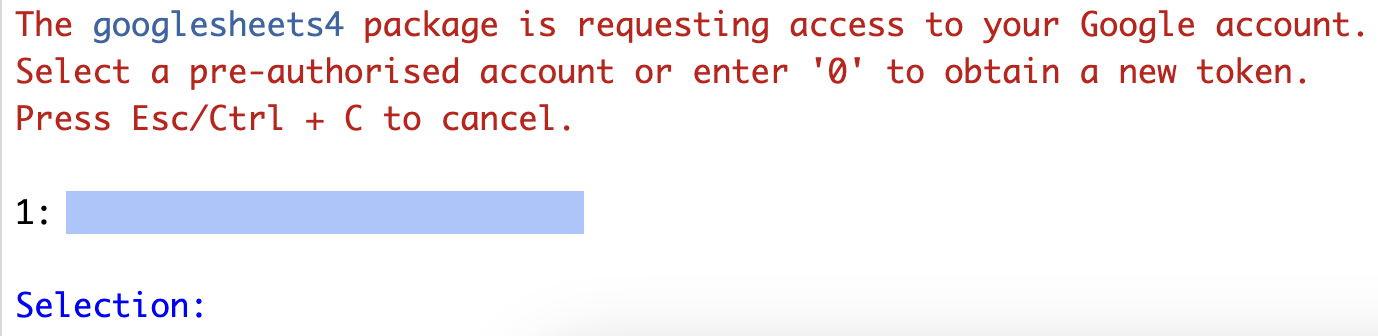
\includegraphics{images/030-_import_data_google_choose.png}

Выбираете (в данном случае у меня только один аккаунт, поэтому пишу
\emph{\texttt{1}} и жму \emph{\texttt{Enter}}).

После этого откроется окно в веб-браузере, в котором Google будет
спрашивать, доверяете ли вы R и готовы ли дать ему доступ к чтению
таблицы (разумеется, отвечаем, что да). Это нужно будет сделать всего
один раз, так что в дальнейшем нажимать в веб-браузере ничего будет не
нужно.

После этого таблица загрузится.

\hypertarget{sec-fastread}{%
\section{Быстрый импорт данных}\label{sec-fastread}}

Чтение табличных данных обычно происходит очень быстро. По крайней мере,
до тех пор пока ваши данные не содержат очень много значений. Если вы
попробуете прочитать с помощью \texttt{read.csv()} таблицу с миллионами
строчками, то заметите, что это происходит довольно медленно. Впрочем,
эта проблема эффективно решается дополнительными пакетами.

\begin{itemize}
\tightlist
\item
  Пакет \texttt{readr} (часть базового tidyverse) предлагает функции,
  очень похожие на стандартные \texttt{read.csv()}, \texttt{read.csv2()}
  и тому подобные, только в названиях используется нижнее подчеркивание:
  \texttt{read\_csv()} и \texttt{read\_csv2()}. Они быстрее и немного
  удобнее, особенно если вы работаете в tidyverse.
\end{itemize}

\begin{Shaded}
\begin{Highlighting}[]
\NormalTok{readr}\SpecialCharTok{::}\FunctionTok{read\_csv}\NormalTok{(}\StringTok{"data/heroes\_information.csv"}\NormalTok{,}
         \AttributeTok{na =} \FunctionTok{c}\NormalTok{(}\StringTok{"{-}"}\NormalTok{, }\StringTok{"{-}99"}\NormalTok{))}
\end{Highlighting}
\end{Shaded}

\begin{verbatim}
New names:
* `` -> `...1`
\end{verbatim}

\begin{verbatim}
Warning: One or more parsing issues, call `problems()` on your data frame for details,
e.g.:
  dat <- vroom(...)
  problems(dat)
\end{verbatim}

\begin{verbatim}
Rows: 734 Columns: 11
-- Column specification --------------------------------------------------------
Delimiter: ","
chr (8): name, Gender, Eye color, Race, Hair color, Publisher, Skin color, A...
dbl (3): ...1, Height, Weight

i Use `spec()` to retrieve the full column specification for this data.
i Specify the column types or set `show_col_types = FALSE` to quiet this message.
\end{verbatim}

\begin{verbatim}
# A tibble: 734 x 11
    ...1 name          Gender `Eye color` Race     `Hair color` Height Publisher
   <dbl> <chr>         <chr>  <chr>       <chr>    <chr>         <dbl> <chr>    
 1     0 A-Bomb        Male   yellow      Human    No Hair         203 Marvel C~
 2     1 Abe Sapien    Male   blue        Icthyo ~ No Hair         191 Dark Hor~
 3     2 Abin Sur      Male   blue        Ungaran  No Hair         185 DC Comics
 4     3 Abomination   Male   green       Human /~ No Hair         203 Marvel C~
 5     4 Abraxas       Male   blue        Cosmic ~ Black            NA Marvel C~
 6     5 Absorbing Man Male   blue        Human    No Hair         193 Marvel C~
 7     6 Adam Monroe   Male   blue        <NA>     Blond            NA NBC - He~
 8     7 Adam Strange  Male   blue        Human    Blond           185 DC Comics
 9     8 Agent 13      Female blue        <NA>     Blond           173 Marvel C~
10     9 Agent Bob     Male   brown       Human    Brown           178 Marvel C~
# i 724 more rows
# i 3 more variables: `Skin color` <chr>, Alignment <chr>, Weight <dbl>
\end{verbatim}

\begin{itemize}
\tightlist
\item
  Пакет \texttt{vroom} - это часть расширенного tidyverse. Это такая
  альтернатива \texttt{readr} из того же tidyverse, но еще быстрее
  (отсюда и название).
\end{itemize}

\begin{Shaded}
\begin{Highlighting}[]
\NormalTok{vroom}\SpecialCharTok{::}\FunctionTok{vroom}\NormalTok{(}\StringTok{"data/heroes\_information.csv"}\NormalTok{)}
\end{Highlighting}
\end{Shaded}

\begin{verbatim}
New names:
Rows: 734 Columns: 11
-- Column specification
-------------------------------------------------------- Delimiter: "," chr
(8): name, Gender, Eye color, Race, Hair color, Publisher, Skin color, A... dbl
(3): ...1, Height, Weight
i Use `spec()` to retrieve the full column specification for this data. i
Specify the column types or set `show_col_types = FALSE` to quiet this message.
* `` -> `...1`
\end{verbatim}

\begin{verbatim}
# A tibble: 734 x 11
    ...1 name          Gender `Eye color` Race     `Hair color` Height Publisher
   <dbl> <chr>         <chr>  <chr>       <chr>    <chr>         <dbl> <chr>    
 1     0 A-Bomb        Male   yellow      Human    No Hair         203 Marvel C~
 2     1 Abe Sapien    Male   blue        Icthyo ~ No Hair         191 Dark Hor~
 3     2 Abin Sur      Male   blue        Ungaran  No Hair         185 DC Comics
 4     3 Abomination   Male   green       Human /~ No Hair         203 Marvel C~
 5     4 Abraxas       Male   blue        Cosmic ~ Black           -99 Marvel C~
 6     5 Absorbing Man Male   blue        Human    No Hair         193 Marvel C~
 7     6 Adam Monroe   Male   blue        -        Blond           -99 NBC - He~
 8     7 Adam Strange  Male   blue        Human    Blond           185 DC Comics
 9     8 Agent 13      Female blue        -        Blond           173 Marvel C~
10     9 Agent Bob     Male   brown       Human    Brown           178 Marvel C~
# i 724 more rows
# i 3 more variables: `Skin color` <chr>, Alignment <chr>, Weight <dbl>
\end{verbatim}

\begin{itemize}
\tightlist
\item
  Пакет \texttt{data.table} - это не просто пакет, а целый фреймворк для
  работы с R, основной конкурент tidyverse. Одна из основных фишек
  \texttt{data.table} - быстрота работы. Это касается не только
  процессинга данных, но и их загрузки и записи. Поэтому некоторые
  используют функции \texttt{data.table} для чтения и записи данных в
  отдельности от всего остального пакета - они даже и называются
  соответствующе: \texttt{fread()} и \texttt{fwrite()}, где \textbf{f}
  означет \textbf{f}ast\footnote{А еще \textbf{f}riendly:
    \texttt{fread()} обычно самостоятельно хорошо угадывает формат
    таблицы на входе. \texttt{vroom} тоже так умеет.}.
\end{itemize}

\begin{Shaded}
\begin{Highlighting}[]
\NormalTok{data.table}\SpecialCharTok{::}\FunctionTok{fread}\NormalTok{(}\StringTok{"data/heroes\_information.csv"}\NormalTok{)}
\end{Highlighting}
\end{Shaded}

\begin{verbatim}
      V1            name Gender Eye color              Race       Hair color
  1:   0          A-Bomb   Male    yellow             Human          No Hair
  2:   1      Abe Sapien   Male      blue     Icthyo Sapien          No Hair
  3:   2        Abin Sur   Male      blue           Ungaran          No Hair
  4:   3     Abomination   Male     green Human / Radiation          No Hair
  5:   4         Abraxas   Male      blue     Cosmic Entity            Black
 ---                                                                        
730: 729 Yellowjacket II Female      blue             Human Strawberry Blond
731: 730            Ymir   Male     white       Frost Giant          No Hair
732: 731            Yoda   Male     brown    Yoda's species            White
733: 732         Zatanna Female      blue             Human            Black
734: 733            Zoom   Male       red                 -            Brown
     Height         Publisher Skin color Alignment Weight
  1:  203.0     Marvel Comics          -      good    441
  2:  191.0 Dark Horse Comics       blue      good     65
  3:  185.0         DC Comics        red      good     90
  4:  203.0     Marvel Comics          -       bad    441
  5:  -99.0     Marvel Comics          -       bad    -99
 ---                                                     
730:  165.0     Marvel Comics          -      good     52
731:  304.8     Marvel Comics      white      good    -99
732:   66.0      George Lucas      green      good     17
733:  170.0         DC Comics          -      good     57
734:  185.0         DC Comics          -       bad     81
\end{verbatim}

Чем же пользоваться среди всего этого многообразия?
\href{https://www.danielecook.com/speeding-up-reading-and-writing-in-r/}{Бенчмарки}\footnote{бенчмаркинг
  --- это тест производительности, в данном случае --- сравнение
  скорости работы конкурирующих пакетов.} показывают, что быстрее всех
\texttt{vroom} и \texttt{data.table}. Если же у вас нет задачи ускорить
работу кода на несколько миллисекунд или прочитать датасет на много
миллионов строк, то стандартного \texttt{read.csv()} (если вы работаете
в базовом R) и \texttt{readr::read\_csv()} (если вы работаете в
tidyverse) должно быть достаточно.

Все перечисленные пакеты повзоляют не только быстро импортировать
данные, но и быстро (и удобно!) экспортировать их:

\begin{Shaded}
\begin{Highlighting}[]
\NormalTok{readr}\SpecialCharTok{::}\FunctionTok{write\_csv}\NormalTok{(dc, }\StringTok{"data/dc\_heroes\_information.csv"}\NormalTok{)}
\NormalTok{readr}\SpecialCharTok{::}\FunctionTok{write\_excel\_csv}\NormalTok{(dc, }\StringTok{"data/dc\_heroes\_information.csv"}\NormalTok{) }\CommentTok{\#Если в Excel возникают проблемы с кодировками при открытии созданного .csv файла, то эта функция решает эти проблемы}
\NormalTok{vroom}\SpecialCharTok{::}\FunctionTok{vroom\_write}\NormalTok{(dc, }\StringTok{"data/dc\_heroes\_information.csv"}\NormalTok{, }\AttributeTok{delim =} \StringTok{","}\NormalTok{)}
\NormalTok{data.table}\SpecialCharTok{::}\FunctionTok{fwrite}\NormalTok{(dc, }\StringTok{"data/dc\_heroes\_information.csv"}\NormalTok{)}
\end{Highlighting}
\end{Shaded}

В плане скорости записи файлов соотношение сил примерно такое же, как и
для чтения: \texttt{vroom} и \texttt{data.table} обгоняют всех, затем
идет \texttt{readr}, и только после него - базовые функции R.

\hypertarget{sec-loops_conditions}{%
\chapter{Условные конструкции и циклы}\label{sec-loops_conditions}}

\hypertarget{sec-sec-if}{%
\section{\texorpdfstring{Выражения \texttt{if}, \texttt{else},
\texttt{else\ if}}{Выражения if, else, else if}}\label{sec-sec-if}}

Стандартная часть практически любого языка программирования --- условные
конструкции. R не исключение. Однако и здесь есть свои особенности.
Начнем с самого простого варианта с одним условием. Выглядеть условная
конcтрукция будет вот так:

\begin{verbatim}
if (условие) выражение
\end{verbatim}

Вот так это будет работать на практике:

\begin{Shaded}
\begin{Highlighting}[]
\NormalTok{number }\OtherTok{\textless{}{-}} \DecValTok{1}
\ControlFlowTok{if}\NormalTok{ (number }\SpecialCharTok{\textgreater{}} \DecValTok{0}\NormalTok{) }\StringTok{"Положительное число"}
\end{Highlighting}
\end{Shaded}

\begin{verbatim}
[1] "Положительное число"
\end{verbatim}

Если выражение (expression) содержит больше одной строчки, то они
объединяются фигурными скобками. Впрочем, использовать их можно, даже
если строчка всего в выражении всего одна.

\begin{Shaded}
\begin{Highlighting}[]
\NormalTok{number }\OtherTok{\textless{}{-}} \DecValTok{1}
\ControlFlowTok{if}\NormalTok{ (number }\SpecialCharTok{\textgreater{}} \DecValTok{0}\NormalTok{) \{}
  \StringTok{"Положительное число"}
\NormalTok{\}}
\end{Highlighting}
\end{Shaded}

\begin{verbatim}
[1] "Положительное число"
\end{verbatim}

В рассмотренной нами конструкции происходит проверка на условие. Если
условие верно\footnote{В принципе, необязательно внутри должна быть
  проверка условий, достаточно просто значения \texttt{TRUE}.}, то
происходит то, что записано в последующем выражении. Если же условие
неверно\footnote{Аналогично, достаточно просто значения \texttt{FALSE}.},
то ничего не происходит.

Оператор \texttt{else} позволяет задавать действие на все остальные
случаи:

\begin{verbatim}
if (условие) выражение else выражение
\end{verbatim}

Работает это так:

\begin{Shaded}
\begin{Highlighting}[]
\NormalTok{number }\OtherTok{\textless{}{-}} \SpecialCharTok{{-}}\DecValTok{3}
\ControlFlowTok{if}\NormalTok{ (number }\SpecialCharTok{\textgreater{}} \DecValTok{0}\NormalTok{) \{}
  \StringTok{"Положительное число"}
\NormalTok{\} }\ControlFlowTok{else}\NormalTok{ \{}
  \StringTok{"Отрицательное число или ноль"}
\NormalTok{\}}
\end{Highlighting}
\end{Shaded}

\begin{verbatim}
[1] "Отрицательное число или ноль"
\end{verbatim}

Иногда нам нужна последовательная проверка на несколько условий. Для
этого есть оператор \texttt{else\ if}. Вот как выглядит ее применение:

\begin{Shaded}
\begin{Highlighting}[]
\NormalTok{number }\OtherTok{\textless{}{-}} \DecValTok{0}
\ControlFlowTok{if}\NormalTok{ (number }\SpecialCharTok{\textgreater{}} \DecValTok{0}\NormalTok{) \{}
  \StringTok{"Положительное число"}
\NormalTok{\} }\ControlFlowTok{else} \ControlFlowTok{if}\NormalTok{ (number }\SpecialCharTok{\textless{}} \DecValTok{0}\NormalTok{)\{}
  \StringTok{"Отрицательное число"}
\NormalTok{\} }\ControlFlowTok{else}\NormalTok{ \{}
  \StringTok{"Ноль"}
\NormalTok{\}}
\end{Highlighting}
\end{Shaded}

\begin{verbatim}
[1] "Ноль"
\end{verbatim}

Как мы помним, R --- язык, в котором векторизация играет большое
значение. Но вот незадача --- условные конструкции не векторизованы в R!
Давайте попробуем применить эти конструкции для вектора значений и
посмотрим, что получится.

\begin{Shaded}
\begin{Highlighting}[]
\NormalTok{numbers }\OtherTok{\textless{}{-}} \SpecialCharTok{{-}}\DecValTok{2}\SpecialCharTok{:}\DecValTok{2}
\ControlFlowTok{if}\NormalTok{ (numbers }\SpecialCharTok{\textgreater{}} \DecValTok{0}\NormalTok{) \{}
  \StringTok{"Положительное число"}
\NormalTok{\} }\ControlFlowTok{else} \ControlFlowTok{if}\NormalTok{ (numbers }\SpecialCharTok{\textless{}} \DecValTok{0}\NormalTok{)\{}
  \StringTok{"Отрицательное число"}
\NormalTok{\} }\ControlFlowTok{else}\NormalTok{ \{}
  \StringTok{"Ноль"}
\NormalTok{\}}
\end{Highlighting}
\end{Shaded}

\begin{verbatim}
Error in if (numbers > 0) {: the condition has length > 1
\end{verbatim}

Ошибка! Однако если у вас более старая версия R (до 4.2.0, апрель 2022),
то вместо ошибки будет учитываться только первое значение вектора
условий: остальные будут игнорироваться, при этом будет выводиться
предупреждение. Как же посчитать для всего вектора сразу?

\begin{tcolorbox}[enhanced jigsaw, leftrule=.75mm, toprule=.15mm, left=2mm, breakable, arc=.35mm, rightrule=.15mm, colback=white, opacityback=0, bottomrule=.15mm]

\textbf{\emph{Полезное:} применение условных конструкций}\vspace{2mm}

Невекторизованная конструкция \emph{if/else/else if} неудобна при работе
с данными, ее практически не используют для обработки данных. В основном
она применяется при написании функций, чтобы проверить конкретное
значение параметра или адекватность данных на входе (см.
Глава~\ref{sec-functional}).

\end{tcolorbox}

\hypertarget{sec-for}{%
\section{\texorpdfstring{Циклы \texttt{for}}{Циклы for}}\label{sec-for}}

Во-первых, можно использовать \texttt{for}. Синтаксис у \texttt{for}
похож на синтаксис условных конструкций.

\begin{verbatim}
for(переменная in последовательность) выражение
\end{verbatim}

Теперь мы можем объединить условные конструкции и \texttt{for}. Немножко
монструозно, но это работает:

\begin{Shaded}
\begin{Highlighting}[]
\ControlFlowTok{for}\NormalTok{ (i }\ControlFlowTok{in}\NormalTok{ numbers) \{}
  \ControlFlowTok{if}\NormalTok{ (i }\SpecialCharTok{\textgreater{}} \DecValTok{0}\NormalTok{) \{}
    \FunctionTok{print}\NormalTok{(}\StringTok{"Положительное число"}\NormalTok{)}
\NormalTok{  \} }\ControlFlowTok{else} \ControlFlowTok{if}\NormalTok{ (i }\SpecialCharTok{\textless{}} \DecValTok{0}\NormalTok{) \{}
    \FunctionTok{print}\NormalTok{(}\StringTok{"Отрицательное число"}\NormalTok{)}
\NormalTok{  \} }\ControlFlowTok{else}\NormalTok{ \{}
    \FunctionTok{print}\NormalTok{(}\StringTok{"Ноль"}\NormalTok{)}
\NormalTok{  \}}
\NormalTok{\}}
\end{Highlighting}
\end{Shaded}

\begin{verbatim}
[1] "Отрицательное число"
[1] "Отрицательное число"
[1] "Ноль"
[1] "Положительное число"
[1] "Положительное число"
\end{verbatim}

\begin{tcolorbox}[enhanced jigsaw, leftrule=.75mm, toprule=.15mm, left=2mm, breakable, arc=.35mm, rightrule=.15mm, colback=white, opacityback=0, bottomrule=.15mm]

\textbf{\emph{Осторожно:} \texttt{print()}}\vspace{2mm}

Чтобы выводить в консоль результат вычислений внутри \texttt{for}, нужно
использовать \texttt{print()}.

\end{tcolorbox}

Здесь стоит отметить, что \texttt{for} используется в R относительно
редко. В подавляющем числе ситуаций использование \texttt{for} можно
избежать. Обычно мы работаем в R с векторами или датафреймами, которые
представляют собой множество относительно независимых наблюдений. Если
мы хотим провести какие-нибудь операции с этими наблюдениями, то они
обычно могут быть выполнены параллельно. Скажем, вы хотите для каждого
испытуемого пересчитать его массу из фунтов в килограммы. Этот пересчет
осуществляется по одинаковой формуле для каждого испытуемого. Эта
формула не изменится из-за того, что какой-то испытуемый слишком большой
или слишком маленький - для следующего испытуемого формула будет
прежняя. Если Вы встречаете подобную задачу (где функцию можно применить
независимо для всех значений), то без цикла \texttt{for} вполне можно
обойтись.

Даже во многих случаях, где расчеты для одной строчки зависят от
расчетов предыдущих строчек, можно обойтись без \texttt{for}
векторизованными функциями, например, \texttt{cumsum()} для подсчета
кумулятивной суммы.

\begin{Shaded}
\begin{Highlighting}[]
\FunctionTok{cumsum}\NormalTok{(}\DecValTok{1}\SpecialCharTok{:}\DecValTok{10}\NormalTok{)}
\end{Highlighting}
\end{Shaded}

\begin{verbatim}
 [1]  1  3  6 10 15 21 28 36 45 55
\end{verbatim}

Если же нет подходящей векторизованной функции, то можно воспользоваться
семейством функций \texttt{apply()} (см. Глава~\ref{sec-apply_f}).

\begin{tcolorbox}[enhanced jigsaw, leftrule=.75mm, toprule=.15mm, left=2mm, breakable, arc=.35mm, rightrule=.15mm, colback=white, opacityback=0, bottomrule=.15mm]

\textbf{\emph{Полезное:} зачем циклы? прост}\vspace{2mm}

После этих объяснений кому-то может показаться странным, что я вообще
упоминаю про эти циклы. Но для кого-то циклы \texttt{for} настолько
привычны, что их полное отсутствие в курсе может показаться еще более
странным. Поэтому лучше от меня, чем на улице.

\end{tcolorbox}

Зачем вообще избегать конструкций \texttt{for}? Некоторые говорят, что
они слишком медленные, и частично это верно, если мы сравниваем с
векторизованными функциями, которые написаны на более низкоуровневых
языках. Но в большинстве случаев низкая скорость \texttt{for} связана с
неправильным использованием этой конструкции. Например, стоит избегать
ситуации, когда на каждой итерации \texttt{for} какой-то объект (вектор,
список, что угодно) изменяется в размере. Лучше будет создать заранее
объект нужного размера, который затем будет наполняться значениями:

\begin{Shaded}
\begin{Highlighting}[]
\NormalTok{numbers\_descriptions }\OtherTok{\textless{}{-}} \FunctionTok{character}\NormalTok{(}\FunctionTok{length}\NormalTok{(numbers)) }\CommentTok{\#создаем строковый вектор с такой же длиной, как и исходный вектор}
\ControlFlowTok{for}\NormalTok{ (i }\ControlFlowTok{in} \DecValTok{1}\SpecialCharTok{:}\FunctionTok{length}\NormalTok{(numbers)) \{}
  \ControlFlowTok{if}\NormalTok{ (numbers[i] }\SpecialCharTok{\textgreater{}} \DecValTok{0}\NormalTok{) \{}
\NormalTok{    numbers\_descriptions[i] }\OtherTok{\textless{}{-}} \StringTok{"Положительное число"}
\NormalTok{  \} }\ControlFlowTok{else} \ControlFlowTok{if}\NormalTok{ (numbers[i] }\SpecialCharTok{\textless{}} \DecValTok{0}\NormalTok{) \{}
\NormalTok{    numbers\_descriptions[i] }\OtherTok{\textless{}{-}} \StringTok{"Отрицательное число"}
\NormalTok{  \} }\ControlFlowTok{else}\NormalTok{ \{}
\NormalTok{    numbers\_descriptions[i] }\OtherTok{\textless{}{-}} \StringTok{"Ноль"}
\NormalTok{  \}}
\NormalTok{\}}
\NormalTok{numbers\_descriptions}
\end{Highlighting}
\end{Shaded}

\begin{verbatim}
[1] "Отрицательное число" "Отрицательное число" "Ноль"               
[4] "Положительное число" "Положительное число"
\end{verbatim}

В общем, при правильном обращении с \texttt{for} особых проблем со
скоростью не будет, хотя векторизованные функции и будут быстрее. Но все
равно это будет громоздкая конструкция, в которой легко ошибиться, и
которую, скорее всего, можно заменить одной короткой строчкой. Кроме
того, без конструкции \texttt{for} код обычно легко превратить в набор
функций, последовательно применяющихся к данным, что мы будем по
максимуму использовать, работая в tidyverse и применяя пайпы (см.
Глава~\ref{sec-pipe}).

\hypertarget{sec-ifelse}{%
\section{\texorpdfstring{Векторизованные условные конструкции: функции
\texttt{ifelse()} и
\texttt{dplyr::case\_when()}}{Векторизованные условные конструкции: функции ifelse() и dplyr::case\_when()}}\label{sec-ifelse}}

Из-за того, что конструкция \emph{if/else/else if} не векторизованная,
она редко используется непосредственно в операциях с данными, обычно она
используется при написании функций (Глава~\ref{sec-create_fun}) и
разработке пакетов.

Альтернативой сочетанию условных конструкций и циклов \texttt{for}
является использование встроенной функции \texttt{ifelse()}. Функция
\texttt{ifelse()} принимает три аргумента:

\begin{enumerate}
\def\labelenumi{\arabic{enumi}.}
\item
  \texttt{test\ =} -- условие (т.е. просто логический вектор, состоящий
  из \texttt{TRUE} и \texttt{FALSE}),
\item
  \texttt{yes\ =} -- что выдавать в случае \texttt{TRUE},
\item
  \texttt{no\ =} -- что выдавать в случае \texttt{FALSE}.
\end{enumerate}

На выходе получается вектор такой же длины, как и изначальный логический
вектор (условие). Это очень похоже на \texttt{ЕСЛИ()} в \emph{Microsoft
Excel.}

\begin{Shaded}
\begin{Highlighting}[]
\FunctionTok{ifelse}\NormalTok{(numbers }\SpecialCharTok{\textgreater{}} \DecValTok{0}\NormalTok{, }\StringTok{"Положительное число"}\NormalTok{, }\StringTok{"Отрицательное число или ноль"}\NormalTok{)}
\end{Highlighting}
\end{Shaded}

\begin{verbatim}
[1] "Отрицательное число или ноль" "Отрицательное число или ноль"
[3] "Отрицательное число или ноль" "Положительное число"         
[5] "Положительное число"         
\end{verbatim}

\begin{tcolorbox}[enhanced jigsaw, leftrule=.75mm, toprule=.15mm, left=2mm, breakable, arc=.35mm, rightrule=.15mm, colback=white, opacityback=0, bottomrule=.15mm]

\textbf{\emph{Полезное:} иногда \texttt{ifelse()} излишен}\vspace{2mm}

Периодически я встречаю у студентов строчку вроде такой:
\texttt{ifelse(условие,\ TRUE,\ FALSE)}. Эта конструкция избыточна, т.к.
получается, что логический вектор из \texttt{TRUE} и \texttt{FALSE}
превращается в абсолютно такой же вектор из \texttt{TRUE} и
\texttt{FALSE} на тех же самых местах. Выходит, что ничего не меняется!

\end{tcolorbox}

\begin{tcolorbox}[enhanced jigsaw, leftrule=.75mm, toprule=.15mm, left=2mm, breakable, arc=.35mm, rightrule=.15mm, colback=white, opacityback=0, bottomrule=.15mm]

\textbf{\emph{Осторожно:} \texttt{NA} в \texttt{ifelse()} превращается в
\texttt{NA}}\vspace{2mm}

\texttt{NA} в условии в \texttt{ifelse()} возвращает \texttt{NA}. Обычно
это именно то поведение, которое вы ожидаете: если в исходном векторе
есть неопределенность, то и на выходе должна остаться неопределенность
на соответствующих позициях.

\end{tcolorbox}

Пакеты \texttt{\{dplyr\}} и \texttt{\{data.table\}} предоставляют более
быстрые и более строгие альтернативы для базовой функции
\texttt{ifelse()} с аналогичным синтаксисом:

\begin{Shaded}
\begin{Highlighting}[]
\NormalTok{dplyr}\SpecialCharTok{::}\FunctionTok{if\_else}\NormalTok{(numbers }\SpecialCharTok{\textgreater{}} \DecValTok{0}\NormalTok{, }\StringTok{"Положительное число"}\NormalTok{, }\StringTok{"Отрицательное число или ноль"}\NormalTok{)}
\end{Highlighting}
\end{Shaded}

\begin{verbatim}
[1] "Отрицательное число или ноль" "Отрицательное число или ноль"
[3] "Отрицательное число или ноль" "Положительное число"         
[5] "Положительное число"         
\end{verbatim}

\begin{Shaded}
\begin{Highlighting}[]
\NormalTok{data.table}\SpecialCharTok{::}\FunctionTok{fifelse}\NormalTok{(numbers }\SpecialCharTok{\textgreater{}} \DecValTok{0}\NormalTok{, }\StringTok{"Положительное число"}\NormalTok{, }\StringTok{"Отрицательное число или ноль"}\NormalTok{)}
\end{Highlighting}
\end{Shaded}

\begin{verbatim}
[1] "Отрицательное число или ноль" "Отрицательное число или ноль"
[3] "Отрицательное число или ноль" "Положительное число"         
[5] "Положительное число"         
\end{verbatim}

Если вы пользуетесь одним из этих пакетов (о них пойдет речь далее ---
см. Глава~\ref{sec-beyond_base_r}, то я советую пользоваться
соотвествующей функцией вместо базового \texttt{ifelse()}.

\begin{tcolorbox}[enhanced jigsaw, leftrule=.75mm, toprule=.15mm, left=2mm, breakable, arc=.35mm, rightrule=.15mm, colback=white, opacityback=0, bottomrule=.15mm]

\textbf{\emph{Осторожно:} возвращение \texttt{NA} может привести к
ошибкам}\vspace{2mm}

Обе функции будут избегать скрытого приведения типов (см.
Глава~\ref{sec-coercion}) и намеренно выдавать ошибку при использовании
разных типов данных в параметрах \texttt{yes\ =} и
\texttt{no\ =}\footnote{В более свежих версиях пакета \texttt{\{dplyr\}}
  разработчики отказались от этой ``строгости'', поэтому \texttt{NA}
  все-таки будут приводиться к нужному типу. Однако
  \texttt{data.table::fifelse()} остался строгим.}. Помните, что
\texttt{NA} по умолчанию --- это логический тип данных, поэтому в этих
функциях нужно использовать \texttt{NA} соответствующего типа
\texttt{NA\_character\_}, \texttt{NA\_integer\_}, \texttt{NA\_real\_},
\texttt{NA\_complex\_} (см. Глава~\ref{sec-na}).

\end{tcolorbox}

У \texttt{ifelse()} тоже есть недостаток: он не может включать в себя
дополнительных условий по типу \texttt{else\ if}. В простых ситуациях
можно вставлять \texttt{ifelse()} внутри \texttt{ifelse()}:

\begin{Shaded}
\begin{Highlighting}[]
\FunctionTok{ifelse}\NormalTok{(numbers }\SpecialCharTok{\textgreater{}} \DecValTok{0}\NormalTok{,}
       \StringTok{"Положительное число"}\NormalTok{,}
       \FunctionTok{ifelse}\NormalTok{(numbers }\SpecialCharTok{\textless{}} \DecValTok{0}\NormalTok{, }\StringTok{"Отрицательное число"}\NormalTok{, }\StringTok{"Ноль"}\NormalTok{))}
\end{Highlighting}
\end{Shaded}

\begin{verbatim}
[1] "Отрицательное число" "Отрицательное число" "Ноль"               
[4] "Положительное число" "Положительное число"
\end{verbatim}

Достаточно симпатичное решение есть в пакете \texttt{dplyr} --- функция
\texttt{case\_when()}, которая работает с использованием формулы:

\begin{Shaded}
\begin{Highlighting}[]
\NormalTok{dplyr}\SpecialCharTok{::}\FunctionTok{case\_when}\NormalTok{(}
\NormalTok{  numbers }\SpecialCharTok{\textgreater{}} \DecValTok{0} \SpecialCharTok{\textasciitilde{}} \StringTok{"Положительное число"}\NormalTok{,}
\NormalTok{  numbers }\SpecialCharTok{\textless{}} \DecValTok{0} \SpecialCharTok{\textasciitilde{}} \StringTok{"Отрицательное число"}\NormalTok{,}
\NormalTok{  numbers }\SpecialCharTok{==} \DecValTok{0} \SpecialCharTok{\textasciitilde{}} \StringTok{"Ноль"}\NormalTok{)}
\end{Highlighting}
\end{Shaded}

\begin{verbatim}
[1] "Отрицательное число" "Отрицательное число" "Ноль"               
[4] "Положительное число" "Положительное число"
\end{verbatim}

Функция \texttt{case\_when()} работает по той же логике, что и
\emph{if/else/else if} конструкция: сначала идет проверка на первое
условие (как первое \emph{if} в конструкции \emph{if/else/else if} ).
Если проверка проходит (то есть в условии получается \texttt{TRUE}), то
соответствующее значение возвращается, а остальные условия не
проверяются. Если же первое условие не выполняется, то идет проверка на
следующее условие (аналог \emph{else if}). Если же и оно не выполняется,
то идет проверка на следующее (следующее \emph{else if}), пока проверка
не пройдет до последнего условия. Можно поставить значение по умолчанию
с помощью параметра \texttt{.default\ =}, которое будет возвращаться,
если все проверки выдали \texttt{FALSE}.

\begin{Shaded}
\begin{Highlighting}[]
\NormalTok{heroes }\OtherTok{\textless{}{-}} \FunctionTok{read.csv}\NormalTok{(}\StringTok{"https://raw.githubusercontent.com/Pozdniakov/tidy\_stats/master/data/heroes\_information.csv"}\NormalTok{, }\AttributeTok{na.strings =} \FunctionTok{c}\NormalTok{(}\StringTok{"NA"}\NormalTok{, }\StringTok{"{-}"}\NormalTok{, }\StringTok{"{-}99"}\NormalTok{))}

\NormalTok{heroes}\SpecialCharTok{$}\NormalTok{weight\_group }\OtherTok{\textless{}{-}}\NormalTok{ dplyr}\SpecialCharTok{::}\FunctionTok{case\_when}\NormalTok{(}
\NormalTok{  heroes}\SpecialCharTok{$}\NormalTok{Weight }\SpecialCharTok{\textgreater{}} \DecValTok{200} \SpecialCharTok{\textasciitilde{}} \StringTok{"overweight"}\NormalTok{, }\CommentTok{\# "if"}
\NormalTok{  heroes}\SpecialCharTok{$}\NormalTok{Weight }\SpecialCharTok{\textgreater{}} \DecValTok{120} \SpecialCharTok{\textasciitilde{}} \StringTok{"somewhat overweight"}\NormalTok{, }\CommentTok{\# "else if"}
\NormalTok{  heroes}\SpecialCharTok{$}\NormalTok{Weight }\SpecialCharTok{\textless{}} \DecValTok{50} \SpecialCharTok{\textasciitilde{}} \StringTok{"underweight"}\NormalTok{, }\CommentTok{\# next "else if"}
  \AttributeTok{.default =} \StringTok{"typical weight"} \CommentTok{\# final "else" }
\NormalTok{) }
\end{Highlighting}
\end{Shaded}

\begin{tcolorbox}[enhanced jigsaw, leftrule=.75mm, toprule=.15mm, left=2mm, breakable, arc=.35mm, rightrule=.15mm, colback=white, opacityback=0, bottomrule=.15mm]

\textbf{Осторожно: не забывайте про запятые}\vspace{2mm}

Будьте внимательны с запятыми! Несмотря на довольно экстравагантный
синтаксис, \texttt{case\_when()} -- это по-прежнему функция, а различные
условия, которые вы прописываете внутри этой функции -- это аргументы
этой функции.

\end{tcolorbox}

Важный момент: если \texttt{ifelse()} возвращает \texttt{NA} на
\texttt{NA} в условии, что обычно нас устраивает (у нас нет данных, что
у нас на входе, следовательно, не знаем, что на выходе), то
\texttt{case\_when()} такого не делает. \texttt{NA} в условии считается
как \texttt{FALSE}, поэтому нужно дополнительно обрабатывать условие для
него. Чтобы на место \texttt{NA} поставить NA, нужно записать вот так:

\begin{Shaded}
\begin{Highlighting}[]
\NormalTok{heroes}\SpecialCharTok{$}\NormalTok{weight\_group }\OtherTok{\textless{}{-}}\NormalTok{ dplyr}\SpecialCharTok{::}\FunctionTok{case\_when}\NormalTok{(}
\NormalTok{  heroes}\SpecialCharTok{$}\NormalTok{Weight }\SpecialCharTok{\textgreater{}} \DecValTok{200} \SpecialCharTok{\textasciitilde{}} \StringTok{"overweight"}\NormalTok{, }\CommentTok{\# "if"}
\NormalTok{  heroes}\SpecialCharTok{$}\NormalTok{Weight }\SpecialCharTok{\textgreater{}} \DecValTok{120} \SpecialCharTok{\textasciitilde{}} \StringTok{"somewhat overweight"}\NormalTok{, }\CommentTok{\# "else if"}
\NormalTok{  heroes}\SpecialCharTok{$}\NormalTok{Weight }\SpecialCharTok{\textless{}} \DecValTok{50} \SpecialCharTok{\textasciitilde{}} \StringTok{"underweight"}\NormalTok{, }\CommentTok{\# next "else if"}
  \FunctionTok{is.na}\NormalTok{(heroes}\SpecialCharTok{$}\NormalTok{Weight) }\SpecialCharTok{\textasciitilde{}} \ConstantTok{NA}\NormalTok{, }\CommentTok{\# one more "else if", maps NA to NA}
  \AttributeTok{.default =} \StringTok{"typical weight"} \CommentTok{\# final "else" }
\NormalTok{  ) }\CommentTok{\# final "else" }
\end{Highlighting}
\end{Shaded}

В \texttt{\{data.table\}} тоже есть свой
(\href{https://themockup.blog/posts/2021-02-13-joins-vs-casewhen-speed-and-memory-tradeoffs/}{более
быстрый}) аналог \texttt{case\_when()} --- функция \texttt{fcase()}.
Синтаксис отличается только тем, что вместо формул используются простые
запятые. То есть первый аргумент -- условие, второй -- значение, которое
возвращается при верности первого аргумента, третий аргумент -- условие,
четвертый -- возвращаемое значение при верности третьего аргумента и
т.д.

\begin{Shaded}
\begin{Highlighting}[]
\NormalTok{data.table}\SpecialCharTok{::}\FunctionTok{fcase}\NormalTok{(}
\NormalTok{  numbers }\SpecialCharTok{\textgreater{}} \DecValTok{0}\NormalTok{, }\StringTok{"Положительное число"}\NormalTok{,}
\NormalTok{  numbers }\SpecialCharTok{\textless{}} \DecValTok{0}\NormalTok{, }\StringTok{"Отрицательное число"}\NormalTok{,}
\NormalTok{  numbers }\SpecialCharTok{==} \DecValTok{0}\NormalTok{, }\StringTok{"Ноль"}\NormalTok{)}
\end{Highlighting}
\end{Shaded}

\begin{verbatim}
[1] "Отрицательное число" "Отрицательное число" "Ноль"               
[4] "Положительное число" "Положительное число"
\end{verbatim}

Задача создания вектора или колонки по множественным условиям из другой
колонки плавно перетекает в задачу объединения двух датафреймов по
единому ключу, и такое решение может оказаться
\href{https://themockup.blog/posts/2021-02-13-joins-vs-casewhen-speed-and-memory-tradeoffs/}{наиболее
быстрым} (см. Глава~\ref{sec-tidy_join}).

\hypertarget{sec-functional}{%
\chapter{Функциональное программирование в R}\label{sec-functional}}

\hypertarget{sec-create_fun}{%
\section{Создание функций}\label{sec-create_fun}}

Поздравляю, сейчас мы выйдем на качественно новый уровень владения R.
Вместо того, чтобы пользоваться теми функциями, которые уже написали за
нас, мы можем сами создавать свои функции! В этом нет ничего сложного.

Синтаксис создания функции внешне похож на создание циклов или условных
конструкций. Мы пишем ключевое слово \texttt{function}, в круглых
скобках обозначаем переменные, с которыми собираемся что-то делать.
Внутри фигурных скобок пишем выражения, которые будут выполняться при
запуске функции. У функции есть свое собственное \textbf{окружение
\emph{(environment)}} --- место, где хранятся переменные. Именно те
объекты, которые мы передаем в скобочках, и будут в окружении, так же
как и ``обычные'' переменные для нас в глобальном окружении. Это
означает, что функция будет искать переменные в первую очередь среди
объектов, которые переданы в круглых скобочках. С ними функция и будет
работать. На выходе функция выдаст то, что вычисляется внутри функции
\texttt{return()}. Если \texttt{return()} появляется в теле функции
несколько раз, то до результат будет возвращаться из той функции
\texttt{return()}, до которой выполнение дошло первым.

\begin{Shaded}
\begin{Highlighting}[]
\NormalTok{pow }\OtherTok{\textless{}{-}} \ControlFlowTok{function}\NormalTok{(x, p) \{}
\NormalTok{  power }\OtherTok{\textless{}{-}}\NormalTok{ x }\SpecialCharTok{\^{}}\NormalTok{ p}
  \FunctionTok{return}\NormalTok{(power)}
\NormalTok{\}}
\FunctionTok{pow}\NormalTok{(}\DecValTok{3}\NormalTok{, }\DecValTok{2}\NormalTok{)}
\end{Highlighting}
\end{Shaded}

\begin{verbatim}
[1] 9
\end{verbatim}

Если функция проработала до конца, а функция \texttt{return()} так и не
встретилась, то возвращается последнее посчитанное значение.

\begin{Shaded}
\begin{Highlighting}[]
\NormalTok{pow }\OtherTok{\textless{}{-}} \ControlFlowTok{function}\NormalTok{(x, p) \{}
\NormalTok{  x }\SpecialCharTok{\^{}}\NormalTok{ p}
\NormalTok{\}}
\FunctionTok{pow}\NormalTok{(}\DecValTok{3}\NormalTok{, }\DecValTok{2}\NormalTok{)}
\end{Highlighting}
\end{Shaded}

\begin{verbatim}
[1] 9
\end{verbatim}

Если в последней строчке будет присвоение, то функция ничего не вернет
обратно. Это очень распространенная ошибка: функция вроде бы работает
правильно, но ничего не возвращает. Нужно писать так, как будто бы в
последней строчке результат выполнения выводится в консоль.

\begin{Shaded}
\begin{Highlighting}[]
\NormalTok{pow }\OtherTok{\textless{}{-}} \ControlFlowTok{function}\NormalTok{(x, p) \{}
\NormalTok{  power }\OtherTok{\textless{}{-}}\NormalTok{ x }\SpecialCharTok{\^{}}\NormalTok{ p }\CommentTok{\#Функция ничего не вернет, потому что в последней строчке присвоение!}
\NormalTok{\}}
\FunctionTok{pow}\NormalTok{(}\DecValTok{3}\NormalTok{, }\DecValTok{2}\NormalTok{) }\CommentTok{\#ничего не возвращается из функции}
\end{Highlighting}
\end{Shaded}

Если функция небольшая, то ее можно записать в одну строчку без фигурных
скобок.

\begin{Shaded}
\begin{Highlighting}[]
\NormalTok{pow }\OtherTok{\textless{}{-}} \ControlFlowTok{function}\NormalTok{(x, p) x }\SpecialCharTok{\^{}}\NormalTok{ p}
\FunctionTok{pow}\NormalTok{(}\DecValTok{3}\NormalTok{, }\DecValTok{2}\NormalTok{) }
\end{Highlighting}
\end{Shaded}

\begin{verbatim}
[1] 9
\end{verbatim}

\begin{tcolorbox}[enhanced jigsaw, leftrule=.75mm, toprule=.15mm, left=2mm, breakable, arc=.35mm, rightrule=.15mm, colback=white, opacityback=0, bottomrule=.15mm]

\textbf{\emph{Для продвинутых:} \texttt{\{\}} -- блок
инструкций}\vspace{2mm}

Вообще, фигурные скобки используются для того, чтобы выполнить серию
команд, но вернуть только результат выполнения последней команды. Такой
набор команд называется \textbf{блоком инструкций \emph{(statements
block)}.} Это можно использовать, чтобы не создавать лишних временных
переменных в глобальном окружении.

\end{tcolorbox}

Мы можем оставить в функции параметры по умолчанию.

\begin{Shaded}
\begin{Highlighting}[]
\NormalTok{pow }\OtherTok{\textless{}{-}} \ControlFlowTok{function}\NormalTok{(x, }\AttributeTok{p =} \DecValTok{2}\NormalTok{) x }\SpecialCharTok{\^{}}\NormalTok{ p}
\FunctionTok{pow}\NormalTok{(}\DecValTok{3}\NormalTok{) }
\end{Highlighting}
\end{Shaded}

\begin{verbatim}
[1] 9
\end{verbatim}

\begin{Shaded}
\begin{Highlighting}[]
\FunctionTok{pow}\NormalTok{(}\DecValTok{3}\NormalTok{, }\DecValTok{3}\NormalTok{) }
\end{Highlighting}
\end{Shaded}

\begin{verbatim}
[1] 27
\end{verbatim}

\begin{tcolorbox}[enhanced jigsaw, leftrule=.75mm, toprule=.15mm, left=2mm, breakable, arc=.35mm, rightrule=.15mm, colback=white, opacityback=0, bottomrule=.15mm]

\textbf{\emph{Для продвинутых:} ленивые вычисления}\vspace{2mm}

В R работают \textbf{ленивые вычисления (lazy evaluations)}. Это
означает, что параметры функций будут только когда они понадобятся, а не
заранее. R будет как самый ленивый прокрастинатор откладывать чтение
данных, пока они не понадобятся в вычислениях. Это приводит к тому, что
если параметр никак не задан, то обнаружится это только при его
непосредственном использовании. Например, эта функция не будет выдавать
ошибку, если мы не зададим параметр
\texttt{we\_will\_not\_use\_this\_parameter\ =}, потому что он нигде не
используется в расчетах.

\begin{Shaded}
\begin{Highlighting}[]
\NormalTok{pow }\OtherTok{\textless{}{-}} \ControlFlowTok{function}\NormalTok{(x, }\AttributeTok{p =} \DecValTok{2}\NormalTok{, we\_will\_not\_use\_this\_parameter) x }\SpecialCharTok{\^{}}\NormalTok{ p}
\FunctionTok{pow}\NormalTok{(}\AttributeTok{x =} \DecValTok{3}\NormalTok{)}
\end{Highlighting}
\end{Shaded}

\begin{verbatim}
[1] 9
\end{verbatim}

\end{tcolorbox}

\hypertarget{sec-sanity_check}{%
\section{Проверка на адекватность}\label{sec-sanity_check}}

Лучший способ не бояться ошибок и предупреждений --- научиться
прописывать их самостоятельно в собственных функциях. Это позволит
понять, что за текстом предупреждений и ошибок, которые у вас возникают,
стоит забота разработчиков о пользователях, которые хотят максимально
обезопасить нас от наших непродуманных действий.

Хорошо написанные функции не только выдают правильный результат на все
возможные адекватные данные на входе, но и не дают получить
правдоподобные результаты при неадекватных входных данных. Как вы уже
знаете, если на входе у вас имеются пропущенные значения, то многие
функции будут в ответ тоже выдавать пропущенные значения. И это вполне
осознанное решение, которое позволяет избегать ситуаций вроде той, когда
\href{https://genomebiology.biomedcentral.com/articles/10.1186/s13059-016-1044-7}{около
одной пятой научных статей по генетике содержало ошибки в приложенных
данных} и замечать пропущенные значения на ранней стадии. Кроме того,
можно проводить \textbf{проверки на адекватность входящих данных
\emph{(sanity check).}}

Разберем \textbf{проверку на адекватность входящих} данных на примере
самодельной функции \texttt{imt()}, которая выдает индекс массы тела,
если на входе задать вес (аргумент \texttt{weight\ =}) в килограммах и
рост (аргумент \texttt{height\ =}) в метрах.

\begin{Shaded}
\begin{Highlighting}[]
\NormalTok{imt }\OtherTok{\textless{}{-}} \ControlFlowTok{function}\NormalTok{(weight, height) weight }\SpecialCharTok{/}\NormalTok{ height }\SpecialCharTok{\^{}} \DecValTok{2}
\end{Highlighting}
\end{Shaded}

Проверим, что функция работает верно:

\begin{Shaded}
\begin{Highlighting}[]
\NormalTok{w }\OtherTok{\textless{}{-}} \FunctionTok{c}\NormalTok{(}\DecValTok{60}\NormalTok{, }\DecValTok{80}\NormalTok{, }\DecValTok{120}\NormalTok{)}
\NormalTok{h }\OtherTok{\textless{}{-}} \FunctionTok{c}\NormalTok{(}\FloatTok{1.6}\NormalTok{, }\FloatTok{1.7}\NormalTok{, }\FloatTok{1.8}\NormalTok{)}
\FunctionTok{imt}\NormalTok{(}\AttributeTok{weight =}\NormalTok{ w, }\AttributeTok{height =}\NormalTok{ h)}
\end{Highlighting}
\end{Shaded}

\begin{verbatim}
[1] 23.43750 27.68166 37.03704
\end{verbatim}

Очень легко перепутать и написать рост в сантиметрах. Было бы здорово
предупредить об этом пользователя, показав ему предупреждающее
сообщение, если рост больше, чем, например, 3. Это можно сделать с
помощью функции \texttt{warning()}.

\begin{Shaded}
\begin{Highlighting}[]
\NormalTok{imt }\OtherTok{\textless{}{-}} \ControlFlowTok{function}\NormalTok{(weight, height) \{}
  \ControlFlowTok{if}\NormalTok{ (}\FunctionTok{any}\NormalTok{(height }\SpecialCharTok{\textgreater{}} \DecValTok{3}\NormalTok{)) }\FunctionTok{warning}\NormalTok{(}\StringTok{"Рост в аргументе height больше 3: возможно, указан рост в сантиметрах, а не в метрах}\SpecialCharTok{\textbackslash{}n}\StringTok{"}\NormalTok{)}
\NormalTok{  weight }\SpecialCharTok{/}\NormalTok{ height }\SpecialCharTok{\^{}} \DecValTok{2}
\NormalTok{\}}
\FunctionTok{imt}\NormalTok{(}\DecValTok{78}\NormalTok{, }\DecValTok{167}\NormalTok{)}
\end{Highlighting}
\end{Shaded}

\begin{verbatim}
Warning in imt(78, 167): Рост в аргументе height больше 3: возможно, указан рост в сантиметрах, а не в метрах
\end{verbatim}

\begin{verbatim}
[1] 0.002796802
\end{verbatim}

В некоторых случаях ответ будет совершенно точно некорректным, хотя
функция все посчитает и выдаст ответ, как будто так и надо. Например,
если какой-то из аргументов функции \texttt{imt()} будет меньше или
равен 0. В этом случае нужно прописать проверку на это условие. Если это
действительно так, то можно поступить еще строже: выдать пользователю
ошибку.

\begin{Shaded}
\begin{Highlighting}[]
\NormalTok{imt }\OtherTok{\textless{}{-}} \ControlFlowTok{function}\NormalTok{(weight, height) \{}
  \ControlFlowTok{if}\NormalTok{ (}\FunctionTok{any}\NormalTok{(weight }\SpecialCharTok{\textless{}=} \DecValTok{0} \SpecialCharTok{|}\NormalTok{ height }\SpecialCharTok{\textless{}=} \DecValTok{0}\NormalTok{)) }\FunctionTok{stop}\NormalTok{(}\StringTok{"Индекс массы тела не может быть посчитан для отрицательных значений"}\NormalTok{)}
  \ControlFlowTok{if}\NormalTok{ (}\FunctionTok{any}\NormalTok{(height }\SpecialCharTok{\textgreater{}} \DecValTok{3}\NormalTok{)) }\FunctionTok{warning}\NormalTok{(}\StringTok{"Рост в аргументе height больше 3: возможно, указан рост в сантиметрах, а не в метрах}\SpecialCharTok{\textbackslash{}n}\StringTok{"}\NormalTok{)}
\NormalTok{  weight }\SpecialCharTok{/}\NormalTok{ height }\SpecialCharTok{\^{}} \DecValTok{2}
\NormalTok{\}}
\FunctionTok{imt}\NormalTok{(}\SpecialCharTok{{-}}\DecValTok{78}\NormalTok{, }\DecValTok{167}\NormalTok{)}
\end{Highlighting}
\end{Shaded}

\begin{verbatim}
Error in imt(-78, 167): Индекс массы тела не может быть посчитан для отрицательных значений
\end{verbatim}

Когда вы попробуете самостоятельно прописывать предупреждения и ошибки в
функциях, то быстро поймете, что ошибки - это вовсе не обязательно
результат того, что где-то что-то сломалось и нужно паниковать. Совсем
даже наоборот, прописанная ошибка - чья-то забота о пользователях,
которых пытаются максимально проинформировать о том, что и почему пошло
не так.

Это естественно в начале работы с R (и вообще с программированием)
избегать ошибок и пугаться их. Конечно, в самом начале обучения большая
часть из них остается непонятной. Но постарайтесь понять текст ошибки,
вспомнить в каких случаях у вас возникала похожая ошибка. Очень часто
этого оказывается достаточно чтобы понять причину ошибки даже если вы
только-только начали изучать R.

Ну а в дальнейшем я советую ознакомиться со
\href{https://adv-r.hadley.nz/debugging.html}{средствами отладки кода в
R} для того, чтобы научиться справляться с ошибками в своем коде на
более продвинутом уровне.

\hypertarget{sec-why_functions}{%
\section{Когда и зачем создавать функции?}\label{sec-why_functions}}

Когда стоит создавать функции? Существует
\href{https://en.wikipedia.org/wiki/Rule_of_three_(computer_programming)}{``правило
трех''} --- если у вас есть три куска очень похожего кода, то самое
время превратить код в функцию. Это очень условное правило, но,
действительно, стоит избегать копипастинга в коде. В этом случае очень
легко ошибиться, а сам код становится нечитаемым.

Есть и другой подход к созданию функций: их стоит создавать не столько
для того, чтобы использовать тот же код снова, сколько для
абстрагирования от того, что происходит в отдельных строчках кода. Если
несколько строчек кода были написаны для того, чтобы решить одну задачу,
которой можно дать понятное название (например, подсчет какой-то
особенной метрики, для которой нет готовой функции в R), то этот код
стоит обернуть в функцию. Если функция работает корректно, то теперь не
нужно думать над тем, что происходит внутри нее. Вы ее можете мысленно
представить как операцию, которая имеет определенный вход и выход ---
как и встроенные функции в R.

Отсюда следует важный вывод, что хорошее название для функции --- это
очень важно. Очень, очень, очень важно.

\hypertarget{sec-functions_objects}{%
\section{Функции как объекты первого
порядка}\label{sec-functions_objects}}

Ранее мы убедились, что арифметические операторы --- это тоже функции.
На самом деле, практически все в R --- это функции. Даже
\texttt{function} --- это функция \texttt{function()}. Даже скобочки
\texttt{(}, \texttt{\{} --- это функции!

А сами функции --- это объекты первого порядка в R. Это означает, что с
функциями вы можете делать практически все то же самое, что и с другими
объектами в R (векторами, датафреймами и т.д.). Небольшой пример,
который может взорвать ваш мозг:

\begin{Shaded}
\begin{Highlighting}[]
\FunctionTok{list}\NormalTok{(mean, min, }\StringTok{\textasciigrave{}}\AttributeTok{\{}\StringTok{\textasciigrave{}}\NormalTok{)}
\end{Highlighting}
\end{Shaded}

\begin{verbatim}
[[1]]
function (x, ...) 
UseMethod("mean")
<bytecode: 0x1359562f8>
<environment: namespace:base>

[[2]]
function (..., na.rm = FALSE)  .Primitive("min")

[[3]]
.Primitive("{")
\end{verbatim}

Мы можем создать список из функций! Зачем --- это другой вопрос, но ведь
можем же! Например, создавать списки из функций может быть удобным для
продвинутых операций в \texttt{across()} в пакете \texttt{\{dplyr\}}
(см. Глава~\ref{sec-tidy_across}).

Еще можно создавать функции внутри функций\footnote{Функция, которая
  создает другие функции, называется \textbf{фабрикой функций}.},
использовать функции в качестве аргументов функций, сохранять функции
как переменные. Пожалуй, самое важное из этого всего - это то, что
функция может быть аргументом в функции. Не просто название функции как
строковая переменная, не результат выполнения функции, а именно сама
функция как объект! Это лежит в основе использования семейства функций
\texttt{apply()}, о которых пойдет речь далее, и многих фишек
\emph{tidyverse.}

\begin{tcolorbox}[enhanced jigsaw, leftrule=.75mm, toprule=.15mm, left=2mm, breakable, arc=.35mm, rightrule=.15mm, colback=white, opacityback=0, bottomrule=.15mm]

\textbf{\emph{Полезное:} а как в Python?}\vspace{2mm}

В Python дело обстоит похожим образом: функции там тоже являются
объектами первого порядка, поэтому все эти фишки функционального
программирования (с поправкой на синтаксис, конечно) будут работать и
там.

\end{tcolorbox}

\hypertarget{sec-apply_f}{%
\section{\texorpdfstring{Семейство функций
\texttt{apply()}}{Семейство функций apply()}}\label{sec-apply_f}}

\hypertarget{sec-apply}{%
\subsection{\texorpdfstring{Применение \texttt{apply()} для
матриц}{Применение apply() для матриц}}\label{sec-apply}}

Семейство? Да, их целое множество: \texttt{apply()},
\texttt{lapply()},\texttt{sapply()},
\texttt{vapply()},\texttt{tapply()},\texttt{mapply()},
\texttt{rapply()}\ldots{} Ладно, не пугайтесь, всех их знать не
придется. Обычно достаточно первых двух-трех. Проще всего пояснить как
они работают на простой матрице с числами:

\begin{Shaded}
\begin{Highlighting}[]
\NormalTok{A }\OtherTok{\textless{}{-}} \FunctionTok{matrix}\NormalTok{(}\DecValTok{1}\SpecialCharTok{:}\DecValTok{12}\NormalTok{, }\DecValTok{3}\NormalTok{, }\DecValTok{4}\NormalTok{)}
\NormalTok{A }
\end{Highlighting}
\end{Shaded}

\begin{verbatim}
     [,1] [,2] [,3] [,4]
[1,]    1    4    7   10
[2,]    2    5    8   11
[3,]    3    6    9   12
\end{verbatim}

\begin{tcolorbox}[enhanced jigsaw, leftrule=.75mm, toprule=.15mm, left=2mm, breakable, arc=.35mm, rightrule=.15mm, colback=white, opacityback=0, bottomrule=.15mm]

\textbf{\emph{Осторожно:} \texttt{apply()} не работает с
датафреймами}\vspace{2mm}

Функция \texttt{apply()} предназначена для работы с матрицами (или
многомерными массивами). Если вы скормите функции \texttt{apply()}
датафрейм, то этот датафрейм будет сначала превращен в матрицу. Главное
отличие матрицы от датафрейма в том, что в матрице все значения одного
типа, поэтому будьте готовы, что сработает имплицитное приведение к
общему типу данных. Например, если среди колонок датафрейма есть хотя бы
одна строковая колонка, то все колонки станут строковыми.

\end{tcolorbox}

Теперь представим, что нам нужно посчитать что-нибудь (например, сумму)
по каждой из строк. С помощью функции \texttt{apply()} вы можете в
буквальном смысле ``применить'' функцию к матрице или датафрейму.
Синтаксис такой: \texttt{apply(X,\ MARGIN,\ FUN,\ ...)}, где \texttt{X}
--- данные, \texttt{MARGIN} это \texttt{1} (для строк), \texttt{2} (для
колонок), \texttt{c(1,2)} для строк и колонок (т.е. для каждого элемента
по отдельности), а \texttt{FUN} --- это функция, которую вы хотите
применить! \texttt{apply()} будет брать строки/колонки из \texttt{X} в
качестве первого аргумента для функции.

\begin{figure}

{\centering 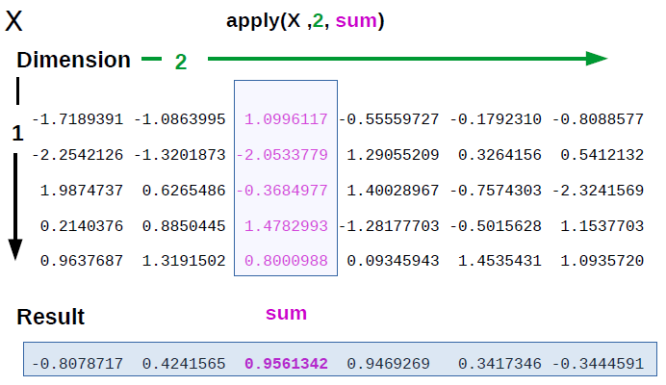
\includegraphics[width=4.16667in,height=\textheight]{images/Apply_function.png}

}

\caption{Визуальное представление функции apply(): выбираем матрицу,
задаем способ итерации (по строкам или столбцам, выбираем функцию,
которая будет применяться на каждом элементе.}

\end{figure}

\begin{tcolorbox}[enhanced jigsaw, leftrule=.75mm, toprule=.15mm, left=2mm, breakable, arc=.35mm, rightrule=.15mm, colback=white, opacityback=0, bottomrule=.15mm]

Заметьте, мы вставляем функцию без скобок и кавычек как аргумент в
функцию. Это как раз тот случай, когда аргументом в функции выступает
сама функция, а не ее название или результат ее выполнения.

\end{tcolorbox}

Давайте разберем на примере:

\begin{Shaded}
\begin{Highlighting}[]
\FunctionTok{apply}\NormalTok{(A, }\DecValTok{1}\NormalTok{, sum) }\CommentTok{\#сумма по каждой строчке}
\end{Highlighting}
\end{Shaded}

\begin{verbatim}
[1] 22 26 30
\end{verbatim}

\begin{Shaded}
\begin{Highlighting}[]
\FunctionTok{apply}\NormalTok{(A, }\DecValTok{2}\NormalTok{, sum) }\CommentTok{\#сумма по каждой колонке}
\end{Highlighting}
\end{Shaded}

\begin{verbatim}
[1]  6 15 24 33
\end{verbatim}

\begin{Shaded}
\begin{Highlighting}[]
\FunctionTok{apply}\NormalTok{(A, }\FunctionTok{c}\NormalTok{(}\DecValTok{1}\NormalTok{,}\DecValTok{2}\NormalTok{), sum) }\CommentTok{\#кхм... сумма каждого элемента}
\end{Highlighting}
\end{Shaded}

\begin{verbatim}
     [,1] [,2] [,3] [,4]
[1,]    1    4    7   10
[2,]    2    5    8   11
[3,]    3    6    9   12
\end{verbatim}

\begin{tcolorbox}[enhanced jigsaw, leftrule=.75mm, toprule=.15mm, left=2mm, breakable, arc=.35mm, rightrule=.15mm, colback=white, opacityback=0, bottomrule=.15mm]

\textbf{\emph{Полезное:} специальные функции для операций над всеми
строками/столбцами}\vspace{2mm}

Конкретно для подсчета сумм и средних по столбцам и строкам в R есть
функции \texttt{colSums()}, \texttt{rowSums()}, \texttt{colMeans()} и
\texttt{rowMeans()}, которые можно использовать как альтернативы
\texttt{apply()} в данном случае.

\end{tcolorbox}

Если же мы хотим прописать дополнительные аргументы для функции, то их
можно перечислить через запятую после функции:

\begin{Shaded}
\begin{Highlighting}[]
\NormalTok{A[}\DecValTok{2}\NormalTok{, }\DecValTok{2}\NormalTok{] }\OtherTok{\textless{}{-}} \ConstantTok{NA}
\NormalTok{A}
\end{Highlighting}
\end{Shaded}

\begin{verbatim}
     [,1] [,2] [,3] [,4]
[1,]    1    4    7   10
[2,]    2   NA    8   11
[3,]    3    6    9   12
\end{verbatim}

\begin{Shaded}
\begin{Highlighting}[]
\FunctionTok{apply}\NormalTok{(A, }\DecValTok{1}\NormalTok{, sum)}
\end{Highlighting}
\end{Shaded}

\begin{verbatim}
[1] 22 NA 30
\end{verbatim}

\begin{Shaded}
\begin{Highlighting}[]
\FunctionTok{apply}\NormalTok{(A, }\DecValTok{1}\NormalTok{, sum, }\AttributeTok{na.rm =} \ConstantTok{TRUE}\NormalTok{)}
\end{Highlighting}
\end{Shaded}

\begin{verbatim}
[1] 22 21 30
\end{verbatim}

\hypertarget{sec-anon_f}{%
\subsection{Анонимные функции}\label{sec-anon_f}}

Что делать, если мы хотим сделать что-то более сложное, чем просто
применить одну функцию? А если функция принимает не первым, а вторым
аргументом данные из матрицы? В этом случае нам помогут
\textbf{анонимные функции \emph{(anonymous function)}}\emph{.}

Анонимные функции - это функции, которые будут использоваться один раз и
без названия.

\begin{tcolorbox}[enhanced jigsaw, leftrule=.75mm, toprule=.15mm, left=2mm, breakable, arc=.35mm, rightrule=.15mm, colback=white, opacityback=0, bottomrule=.15mm]

\textbf{\emph{Полезное:} а как в Python?}\vspace{2mm}

Питонистам знакомо понятие \textbf{лямбда-функций}. Да, это то же самое.

\end{tcolorbox}

Например, мы можем посчитать общее количество знаков по строкам и
столбцам без называния этой функции:

\begin{Shaded}
\begin{Highlighting}[]
\NormalTok{B }\OtherTok{\textless{}{-}} \FunctionTok{matrix}\NormalTok{(}\FunctionTok{c}\NormalTok{(}\StringTok{"Всем"}\NormalTok{, }\StringTok{"привет"}\NormalTok{, }\StringTok{"Я"}\NormalTok{, }\StringTok{"строковая"}\NormalTok{, }\StringTok{"матрица"}\NormalTok{, }\StringTok{"и"}\NormalTok{, }\StringTok{"такое"}\NormalTok{, }\StringTok{"тоже"}\NormalTok{, }\StringTok{"бывает"}\NormalTok{), }\AttributeTok{nrow =} \DecValTok{3}\NormalTok{)}
\FunctionTok{apply}\NormalTok{(B, }\DecValTok{1}\NormalTok{, }\ControlFlowTok{function}\NormalTok{(x) }\FunctionTok{sum}\NormalTok{(}\FunctionTok{nchar}\NormalTok{(x)))}
\end{Highlighting}
\end{Shaded}

\begin{verbatim}
[1] 18 17  8
\end{verbatim}

\begin{Shaded}
\begin{Highlighting}[]
\FunctionTok{apply}\NormalTok{(B, }\DecValTok{2}\NormalTok{, }\ControlFlowTok{function}\NormalTok{(x) }\FunctionTok{sum}\NormalTok{(}\FunctionTok{nchar}\NormalTok{(x)))}
\end{Highlighting}
\end{Shaded}

\begin{verbatim}
[1] 11 17 15
\end{verbatim}

Начиная с R 4.1.0 (май 2021) можно использовать сокращенный вариант
написания анонимных функций с \texttt{\textbackslash{}} вместо ключевого
слова \texttt{function}:

\begin{Shaded}
\begin{Highlighting}[]
\FunctionTok{apply}\NormalTok{(B, }\DecValTok{1}\NormalTok{, \textbackslash{}(x) }\FunctionTok{sum}\NormalTok{(}\FunctionTok{nchar}\NormalTok{(x)))}
\end{Highlighting}
\end{Shaded}

\begin{verbatim}
[1] 18 17  8
\end{verbatim}

\begin{Shaded}
\begin{Highlighting}[]
\FunctionTok{apply}\NormalTok{(B, }\DecValTok{2}\NormalTok{, \textbackslash{}(x) }\FunctionTok{sum}\NormalTok{(}\FunctionTok{nchar}\NormalTok{(x)))}
\end{Highlighting}
\end{Shaded}

\begin{verbatim}
[1] 11 17 15
\end{verbatim}

\begin{tcolorbox}[enhanced jigsaw, leftrule=.75mm, toprule=.15mm, left=2mm, breakable, arc=.35mm, rightrule=.15mm, colback=white, opacityback=0, bottomrule=.15mm]

\textbf{\emph{Полезное:} аргументы анонимной функции}\vspace{2mm}

Как и в случае с обычной функцией, в качестве \texttt{x} выступает
объект, с которым мы хотим что-то сделать, а дальше следует функция,
которую мы собираемся применить к \texttt{х}. Можно использовать не
\texttt{х}, а что угодно, как и в обычных функциях:

\begin{Shaded}
\begin{Highlighting}[]
\FunctionTok{apply}\NormalTok{(B, }\DecValTok{1}\NormalTok{, }\ControlFlowTok{function}\NormalTok{(whatevername) }\FunctionTok{sum}\NormalTok{(}\FunctionTok{nchar}\NormalTok{(whatevername)))}
\end{Highlighting}
\end{Shaded}

\begin{verbatim}
[1] 18 17  8
\end{verbatim}

\end{tcolorbox}

\hypertarget{sec-apply_other}{%
\subsection{\texorpdfstring{Другие функции семейства
\texttt{apply()}}{Другие функции семейства apply()}}\label{sec-apply_other}}

ОК, с \texttt{apply()} разобрались. А что с остальными? Некоторые из
функций семейства \texttt{*apply()} еще проще и не требуют индексов,
например, \texttt{lapply()} (для применения к каждому элементу списка) и
\texttt{sapply()} - упрощенная версия \texttt{lapply()}, которая
пытается по возможности ``упростить'' результат до вектора или матрицы.

\begin{Shaded}
\begin{Highlighting}[]
\NormalTok{some\_list }\OtherTok{\textless{}{-}} \FunctionTok{list}\NormalTok{(}\AttributeTok{some =} \DecValTok{1}\SpecialCharTok{:}\DecValTok{10}\NormalTok{, }\AttributeTok{list =}\NormalTok{ letters)}
\FunctionTok{lapply}\NormalTok{(some\_list, length)}
\end{Highlighting}
\end{Shaded}

\begin{verbatim}
$some
[1] 10

$list
[1] 26
\end{verbatim}

\begin{Shaded}
\begin{Highlighting}[]
\FunctionTok{sapply}\NormalTok{(some\_list, length)}
\end{Highlighting}
\end{Shaded}

\begin{verbatim}
some list 
  10   26 
\end{verbatim}

\begin{tcolorbox}[enhanced jigsaw, leftrule=.75mm, toprule=.15mm, left=2mm, breakable, arc=.35mm, rightrule=.15mm, colback=white, opacityback=0, bottomrule=.15mm]

\textbf{\emph{Осторожно:} такой непредсказуемый
\texttt{sapply()}}\vspace{2mm}

Достаточно сложно предсказать, в каких именно случаях будет произведено
упрощение, а в каких нет. Поэтому \texttt{sapply()} удобен в
исследовании данных, но использовать эту функцию в скриптах не очень
рекомендуется. Один из вариантов решения этой проблемы --- это функция
\texttt{vapply()}, которая позволяет управлять результатом
\texttt{lapply()}, но гораздо более красиво эта проблема решена в пакете
\texttt{\{purrr\}} (см. Глава~\ref{sec-purrr} ).

\end{tcolorbox}

Использование \texttt{sapply()} на векторе приводит к тем же
результатам, что и просто применить векторизованную функцию обычным
способом.

\begin{Shaded}
\begin{Highlighting}[]
\FunctionTok{sapply}\NormalTok{(}\DecValTok{1}\SpecialCharTok{:}\DecValTok{10}\NormalTok{, sqrt)}
\end{Highlighting}
\end{Shaded}

\begin{verbatim}
 [1] 1.000000 1.414214 1.732051 2.000000 2.236068 2.449490 2.645751 2.828427
 [9] 3.000000 3.162278
\end{verbatim}

\begin{Shaded}
\begin{Highlighting}[]
\FunctionTok{sqrt}\NormalTok{(}\DecValTok{1}\SpecialCharTok{:}\DecValTok{10}\NormalTok{)}
\end{Highlighting}
\end{Shaded}

\begin{verbatim}
 [1] 1.000000 1.414214 1.732051 2.000000 2.236068 2.449490 2.645751 2.828427
 [9] 3.000000 3.162278
\end{verbatim}

Зачем вообще тогда нужен \texttt{sapply()}, если мы можем просто
применить векторизованную функцию? Ключевое слово здесь
\emph{векторизованная} функция. Если функция не векторизована, то
\texttt{sapply()} становится удобным вариантом для того, чтобы избежать
итерирования с помощью циклов \texttt{for}.

\begin{tcolorbox}[enhanced jigsaw, leftrule=.75mm, toprule=.15mm, left=2mm, breakable, arc=.35mm, rightrule=.15mm, colback=white, opacityback=0, bottomrule=.15mm]

\textbf{\emph{Для продвинутых:} \texttt{Vectorize()}}\vspace{2mm}

Еще одна альтернатива - это векторизация невекторизованной функции с
помощью \texttt{Vectorize()}. Эта функция просто оборачивает функцию
одним из вариантов \texttt{apply()}. Обратите внимание: функция
\texttt{Vectorize()} в качестве аргумента принимает функцию и возвращает
тоже функцию!

\end{tcolorbox}

Можно применять функции \texttt{lapply()} и \texttt{sapply()} на
датафреймах. Поскольку фактически датафрейм - это список из векторов
одинаковой длины (см. Глава~\ref{sec-df}), то итерироваться эти функции
будут по колонкам:

\begin{Shaded}
\begin{Highlighting}[]
\NormalTok{heroes }\OtherTok{\textless{}{-}} \FunctionTok{read.csv}\NormalTok{(}\StringTok{"https://raw.githubusercontent.com/Pozdniakov/tidy\_stats/master/data/heroes\_information.csv"}\NormalTok{, }
                   \AttributeTok{na.strings =} \FunctionTok{c}\NormalTok{(}\StringTok{"{-}"}\NormalTok{, }\StringTok{"{-}99"}\NormalTok{))}
\FunctionTok{sapply}\NormalTok{(heroes, class)}
\end{Highlighting}
\end{Shaded}

\begin{verbatim}
          X        name      Gender   Eye.color        Race  Hair.color 
  "integer" "character" "character" "character" "character" "character" 
     Height   Publisher  Skin.color   Alignment      Weight 
  "numeric" "character" "character" "character"   "integer" 
\end{verbatim}

Еще одна функция из семейства \texttt{apply()} - функция
\texttt{replicate()} - самый простой способ повторить одну и ту же
операцию много раз. Обычно эта функция используется при симуляции данных
и моделировании. Например, давайте сделаем выборку из логнормального
распределения (подробнее про распределения см. в
Глава~\ref{sec-distributions}):

\begin{Shaded}
\begin{Highlighting}[]
\NormalTok{samp }\OtherTok{\textless{}{-}} \FunctionTok{rlnorm}\NormalTok{(}\DecValTok{30}\NormalTok{)}
\FunctionTok{hist}\NormalTok{(samp)}
\end{Highlighting}
\end{Shaded}

\begin{figure}[H]

{\centering 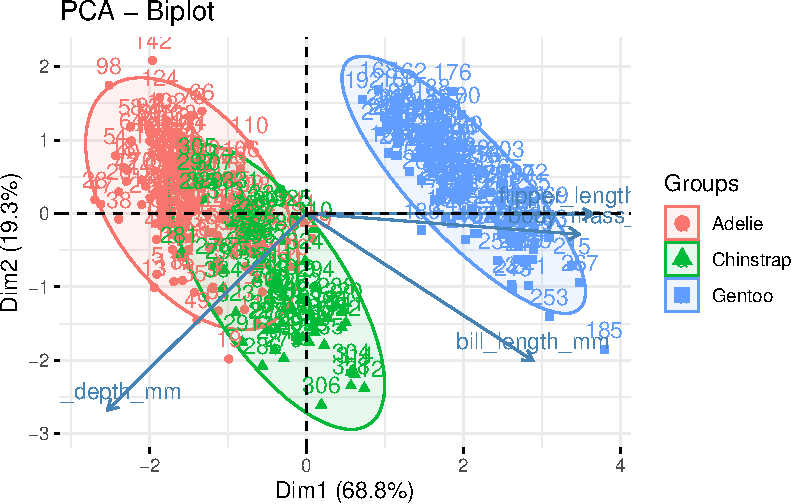
\includegraphics{050-functional_files/figure-pdf/unnamed-chunk-21-1.pdf}

}

\end{figure}

А теперь давайте сделаем 1000 таких выборок и из каждой возьмем среднее:

\begin{Shaded}
\begin{Highlighting}[]
\NormalTok{sampdist }\OtherTok{\textless{}{-}} \FunctionTok{replicate}\NormalTok{(}\DecValTok{1000}\NormalTok{, }\FunctionTok{mean}\NormalTok{(}\FunctionTok{rlnorm}\NormalTok{(}\DecValTok{30}\NormalTok{)))}
\FunctionTok{hist}\NormalTok{(sampdist)}
\end{Highlighting}
\end{Shaded}

\begin{figure}[H]

{\centering 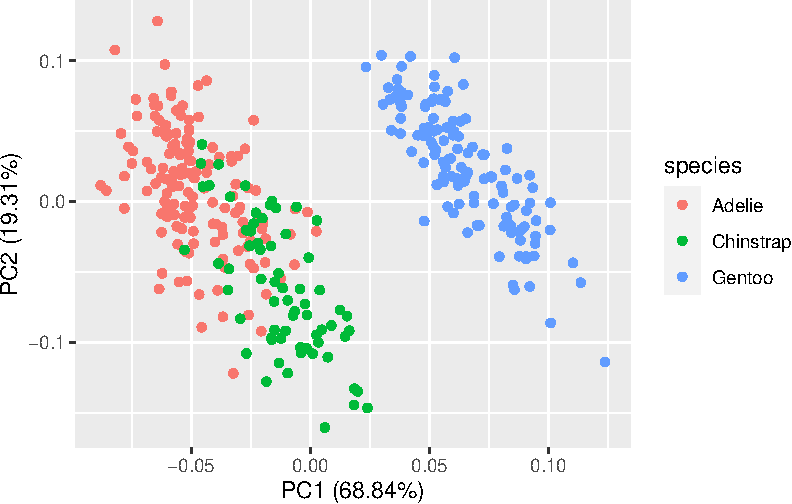
\includegraphics{050-functional_files/figure-pdf/unnamed-chunk-22-1.pdf}

}

\end{figure}

Про функции для генерации случайных чисел и про визуализацию будет в
следующих главах: Глава~\ref{sec-distributions} и Глава~\ref{sec-r_vis}
соответственно.

\begin{tcolorbox}[enhanced jigsaw, leftrule=.75mm, toprule=.15mm, left=2mm, breakable, arc=.35mm, rightrule=.15mm, colback=white, opacityback=0, bottomrule=.15mm]

\textbf{\emph{Для продвинутых:} больше \texttt{apply()}}\vspace{2mm}

Если хотите познакомиться с семейством \texttt{apply()} чуточку ближе,
то рекомендую
\href{https://www.datacamp.com/community/tutorials/r-tutorial-apply-family}{вот
этот туториал}.

\end{tcolorbox}

В заключение стоит сказать, что семейство функций \texttt{apply()} ---
это очень сильное колдунство, но в \emph{tidyverse} оно практически
полностью перекрывается функциями из пакета \texttt{\{purrr\}}, за
исключением самого \texttt{apply()} и некоторых других функций, которые
работают с матрицами и массивами (\emph{tidyverse} с ними принципиально
не дружит). Впрочем, если вы поняли логику \texttt{apply()}, то при
желании вы легко сможете переключиться на альтернативы из пакета
\texttt{\{purrr\}} (см. Глава~\ref{sec-purrr}).

\part{Tidyverse}

\hypertarget{sec-beyond_base_r}{%
\chapter{За пределами base R: tidyverse и
data.table}\label{sec-beyond_base_r}}

Как вы уже, наверное, убедились, базовый R умеет очень много, в том
числе и для работы с данными. Однако какие-то операции все равно
выполнить довольно непросто.

Возьмем, например, задачу агрегации: вам нужно посчитать средний рост
супергероев отдельно для мужчин и для женщин (а еще и для \texttt{NA},
за компанию). Три группы еще ничего, а если бы их было 10, 50 или 200? В
базовом R для этого есть специальная функция \texttt{aggregate()}, но
она довольно неудобная.

Поэтому стали появляться пакеты, которые пытаются сделать агрегацию и
другие непростые операции максимально безболезненными способами.
Основных таких пакетов два: \texttt{\{data.table\}} и
\texttt{\{tidyverse\}}. Это огромные пакеты, которые очень сильно
изменяют работу в R, в том числе в плане стиля и используемой парадигмы.
Тем не менее, в основе своей стоит все то, что мы прошли раньше.

\hypertarget{sec-dt_approach}{%
\section{\texorpdfstring{Подход
\texttt{\{data.table\}}}{Подход \{data.table\}}}\label{sec-dt_approach}}

\texttt{\{data.table\}} -- это распространенный пакет, который позволяет
анализировать датафреймы максимально быстро и с помощью очень
лаконичного кода.

\begin{Shaded}
\begin{Highlighting}[]
\FunctionTok{install.packages}\NormalTok{(}\StringTok{"data.table"}\NormalTok{)}
\end{Highlighting}
\end{Shaded}

Давайте импортируем наш набор данных про супергероев. Для этого
воспользуемся функцией \texttt{fread()} из пакета
\texttt{\{data.table\}}. Эта функция нам уже знакома как функция для
импорта больших наборов данных Глава~\ref{sec-fastread}.

\emph{``f''} в \texttt{fread()} означает \emph{``\textbf{f}ast and
\textbf{f}riendly''}: эта функция очень быстрая и довольно хорошо
угадывает формат текстовой таблицы.

\begin{Shaded}
\begin{Highlighting}[]
\FunctionTok{library}\NormalTok{(data.table)}
\NormalTok{heroes\_dt }\OtherTok{\textless{}{-}}
  \FunctionTok{fread}\NormalTok{(}
    \StringTok{"https://raw.githubusercontent.com/Pozdniakov/tidy\_stats/master/data/heroes\_information.csv"}\NormalTok{,}
    \AttributeTok{na.strings =} \FunctionTok{c}\NormalTok{(}\StringTok{"NA"}\NormalTok{, }\StringTok{"{-}"}\NormalTok{, }\StringTok{"{-}99"}\NormalTok{)}
\NormalTok{  )}
\end{Highlighting}
\end{Shaded}

Функция \texttt{fread()} создает не просто датафрейм, а
\textbf{дататейбл}:

\begin{Shaded}
\begin{Highlighting}[]
\NormalTok{heroes\_dt}
\end{Highlighting}
\end{Shaded}

\begin{verbatim}
      V1            name Gender Eye color              Race       Hair color
  1:   0          A-Bomb   Male    yellow             Human          No Hair
  2:   1      Abe Sapien   Male      blue     Icthyo Sapien          No Hair
  3:   2        Abin Sur   Male      blue           Ungaran          No Hair
  4:   3     Abomination   Male     green Human / Radiation          No Hair
  5:   4         Abraxas   Male      blue     Cosmic Entity            Black
 ---                                                                        
730: 729 Yellowjacket II Female      blue             Human Strawberry Blond
731: 730            Ymir   Male     white       Frost Giant          No Hair
732: 731            Yoda   Male     brown    Yoda's species            White
733: 732         Zatanna Female      blue             Human            Black
734: 733            Zoom   Male       red              <NA>            Brown
     Height         Publisher Skin color Alignment Weight
  1:  203.0     Marvel Comics       <NA>      good    441
  2:  191.0 Dark Horse Comics       blue      good     65
  3:  185.0         DC Comics        red      good     90
  4:  203.0     Marvel Comics       <NA>       bad    441
  5:     NA     Marvel Comics       <NA>       bad     NA
 ---                                                     
730:  165.0     Marvel Comics       <NA>      good     52
731:  304.8     Marvel Comics      white      good     NA
732:   66.0      George Lucas      green      good     17
733:  170.0         DC Comics       <NA>      good     57
734:  185.0         DC Comics       <NA>       bad     81
\end{verbatim}

\begin{Shaded}
\begin{Highlighting}[]
\FunctionTok{class}\NormalTok{(heroes\_dt)}
\end{Highlighting}
\end{Shaded}

\begin{verbatim}
[1] "data.table" "data.frame"
\end{verbatim}

\textbf{Дататейбл} -- это ``улучшенный'' датафрейм: с ним работают все
те функции, которые мы применяли для датафрейма, специальные функции для
дататейбла, а что-то работает немного по-другому по сравнению с
датафреймом. Например, оператор \texttt{{[}}, т.е. квадратные скобки.

Давайте посмотрим по-внимательнее как это происходит на примере расчета
среднего роста супергероев, группируя по полу:

\begin{Shaded}
\begin{Highlighting}[]
\NormalTok{heroes\_dt[, }\FunctionTok{mean}\NormalTok{(Height, }\AttributeTok{na.rm =} \ConstantTok{TRUE}\NormalTok{), by }\OtherTok{=}\NormalTok{ Gender]}
\end{Highlighting}
\end{Shaded}

\begin{verbatim}
   Gender       V1
1:   Male 191.9749
2: Female 174.6840
3:   <NA> 177.0667
\end{verbatim}

Сразу уже усложним задачу: возьмем только хороших (у кого в колонке
\texttt{Alignment} стоит \texttt{"good"}), а потом еще отсортируем по
среднему росту.

\begin{Shaded}
\begin{Highlighting}[]
\NormalTok{heroes\_dt[Alignment }\SpecialCharTok{==} \StringTok{"good"}\NormalTok{, }
\NormalTok{          .(}\AttributeTok{mean\_height =} \FunctionTok{mean}\NormalTok{(Height, }\AttributeTok{na.rm =} \ConstantTok{TRUE}\NormalTok{)), }
\NormalTok{          by }\OtherTok{=}\NormalTok{ Gender][}
            \FunctionTok{order}\NormalTok{(}\SpecialCharTok{{-}}\NormalTok{mean\_height)}
\NormalTok{          ]}
\end{Highlighting}
\end{Shaded}

\begin{verbatim}
   Gender mean_height
1:   Male    188.9601
2:   <NA>    179.5000
3: Female    174.7607
\end{verbatim}

Уух! Выглядит монструозно, да? Зато как мы все сделали используя
минимальное количество знаков. Заметьте, что здесь необычного для нас:

\begin{itemize}
\item
  Не нужно прописывать \texttt{heroes\_dt\$Alignment}, поиск переменной
  будет начинаться с колонок дататейбла.
\item
  Там, где мы раньше выбирали колонки, мы еще и расчеты можем вести.
\item
  Внутри квадратных скобок появилась вторая запятая, т.е. третье поле, в
  котором мы прописали группировку.
\item
  Несколько операций прописываются путем соединения квадратных скобочек,
  код превращается в эдакий паровозик\footnote{Это работает и в базовом
    R, но именно в \texttt{\{data.table\}} это очень частая конструкция.}.
\end{itemize}

И это не все отличия!

На \href{https://rdatatable.gitlab.io/data.table/}{сайте пакета
\texttt{\{data.table\}}} особенно уделяется вниманию скорости
\texttt{\{data.table\}}, приводя в качестве доказательства
\href{https://h2oai.github.io/db-benchmark/}{бэнчмарк}, где сравниваются
по скорости различные инструменты для работы с данными.
\texttt{\{data.table\}} почти на порядок обгоняет как
\texttt{\{dplyr\}}, так и питоновский \emph{pandas} -- самый
используемый пакет для анализа данных в \emph{Python}.

Разработчики \texttt{\{data.table\}} делают особый акцент на
``консервативности'' пакета: у него нет никаких зависимостей (в этом
плане пакет \texttt{\{data.table\}} обгоняет большинство российских
экспатов в Тбилиси), ему достаточно очень старой версии R,
функционирование пакета не будет ломаться из-за выкинутых устаревших
функций. В общем, \texttt{\{data.table\}} очень суров и уважаем
программистами. Он и не особо пытается понравиться рядовым
пользователям. Зато освоив его, вы сможете творить магию: то, что с
помощью базового R, \emph{tidyverse} или Python будет выполняться очень
долго (если выполнится вообще), \texttt{\{data.table\}} сможет сделать
гораздо быстрее, иногда в десятки и сотни раз!

Очень сильно, не правда ли? Чем же может ответить \emph{tidyverse}?

\hypertarget{sec-tidy_approach}{%
\section{Подход tidyverse}\label{sec-tidy_approach}}

Давайте посмотрим, как будет выглядеть решение тех же задач (отбор строк
по условию, агрегация и сортировка) в \emph{tidyverse}.

\begin{Shaded}
\begin{Highlighting}[]
\FunctionTok{install.packages}\NormalTok{(}\StringTok{"tidyverse"}\NormalTok{)}
\end{Highlighting}
\end{Shaded}

\begin{Shaded}
\begin{Highlighting}[]
\FunctionTok{library}\NormalTok{(tidyverse)}
\end{Highlighting}
\end{Shaded}

\begin{verbatim}
-- Attaching packages --------------------------------------- tidyverse 1.3.2 --
v ggplot2 3.4.2     v purrr   1.0.1
v tibble  3.2.1     v dplyr   1.1.2
v tidyr   1.3.0     v stringr 1.5.0
v readr   2.1.3     v forcats 1.0.0
-- Conflicts ------------------------------------------ tidyverse_conflicts() --
x dplyr::between()   masks data.table::between()
x dplyr::filter()    masks stats::filter()
x dplyr::first()     masks data.table::first()
x dplyr::lag()       masks stats::lag()
x dplyr::last()      masks data.table::last()
x purrr::transpose() masks data.table::transpose()
\end{verbatim}

Не пугайтесь сообщений, все в порядке. Во-первых, пакет
\texttt{\{tidyverse\}} -- это не просто пакет, а ``пакет с пакетами''
(да-да, как у вас дома), который подключает сразу несколько других
пакетов, которые составляют \emph{ядро tidyverse}. Список и версии этих
пакетов \texttt{\{tidyverse\}} выводит при подключении. Разные пакеты
\emph{tidyverse} мы очень детально разберем позже
(Глава~\ref{sec-tidy_intro} ), а сейчас просто посмотрите, как это все
выглядит.

\begin{Shaded}
\begin{Highlighting}[]
\NormalTok{heroes\_tbl }\OtherTok{\textless{}{-}} \FunctionTok{read\_csv}\NormalTok{(}\StringTok{"https://raw.githubusercontent.com/Pozdniakov/tidy\_stats/master/data/heroes\_information.csv"}\NormalTok{,}
    \AttributeTok{na =} \FunctionTok{c}\NormalTok{(}\StringTok{"NA"}\NormalTok{, }\StringTok{"{-}"}\NormalTok{, }\StringTok{"{-}99"}\NormalTok{))}
\end{Highlighting}
\end{Shaded}

\begin{verbatim}
New names:
* `` -> `...1`
\end{verbatim}

\begin{verbatim}
Warning: One or more parsing issues, call `problems()` on your data frame for details,
e.g.:
  dat <- vroom(...)
  problems(dat)
\end{verbatim}

\begin{verbatim}
Rows: 734 Columns: 11
-- Column specification --------------------------------------------------------
Delimiter: ","
chr (8): name, Gender, Eye color, Race, Hair color, Publisher, Skin color, A...
dbl (3): ...1, Height, Weight

i Use `spec()` to retrieve the full column specification for this data.
i Specify the column types or set `show_col_types = FALSE` to quiet this message.
\end{verbatim}

Функция \texttt{read\_csv()} (не путать с функцией из базового R --
\texttt{read.csv()}!) возвращает \textbf{тиббл} -- ``улучшенный''
датафрейм, примерно как это было с дататейблом.

\begin{Shaded}
\begin{Highlighting}[]
\NormalTok{heroes\_tbl}
\end{Highlighting}
\end{Shaded}

\begin{verbatim}
# A tibble: 734 x 11
    ...1 name          Gender `Eye color` Race     `Hair color` Height Publisher
   <dbl> <chr>         <chr>  <chr>       <chr>    <chr>         <dbl> <chr>    
 1     0 A-Bomb        Male   yellow      Human    No Hair         203 Marvel C~
 2     1 Abe Sapien    Male   blue        Icthyo ~ No Hair         191 Dark Hor~
 3     2 Abin Sur      Male   blue        Ungaran  No Hair         185 DC Comics
 4     3 Abomination   Male   green       Human /~ No Hair         203 Marvel C~
 5     4 Abraxas       Male   blue        Cosmic ~ Black            NA Marvel C~
 6     5 Absorbing Man Male   blue        Human    No Hair         193 Marvel C~
 7     6 Adam Monroe   Male   blue        <NA>     Blond            NA NBC - He~
 8     7 Adam Strange  Male   blue        Human    Blond           185 DC Comics
 9     8 Agent 13      Female blue        <NA>     Blond           173 Marvel C~
10     9 Agent Bob     Male   brown       Human    Brown           178 Marvel C~
# i 724 more rows
# i 3 more variables: `Skin color` <chr>, Alignment <chr>, Weight <dbl>
\end{verbatim}

\begin{Shaded}
\begin{Highlighting}[]
\FunctionTok{class}\NormalTok{(heroes\_tbl)}
\end{Highlighting}
\end{Shaded}

\begin{verbatim}
[1] "spec_tbl_df" "tbl_df"      "tbl"         "data.frame" 
\end{verbatim}

Теперь же сделаем то же самое с нашими данными, что мы делали с помощью
\texttt{\{data.table\}}:

\begin{Shaded}
\begin{Highlighting}[]
\NormalTok{heroes\_tbl }\SpecialCharTok{\%\textgreater{}\%}
  \FunctionTok{filter}\NormalTok{(Alignment }\SpecialCharTok{==} \StringTok{"good"}\NormalTok{) }\SpecialCharTok{\%\textgreater{}\%}
  \FunctionTok{group\_by}\NormalTok{(Gender) }\SpecialCharTok{\%\textgreater{}\%}
  \FunctionTok{summarise}\NormalTok{(}\AttributeTok{mean\_height =} \FunctionTok{mean}\NormalTok{(Height, }\AttributeTok{na.rm =} \ConstantTok{TRUE}\NormalTok{)) }\SpecialCharTok{\%\textgreater{}\%}
  \FunctionTok{arrange}\NormalTok{(}\FunctionTok{desc}\NormalTok{(mean\_height))}
\end{Highlighting}
\end{Shaded}

\begin{verbatim}
# A tibble: 3 x 2
  Gender mean_height
  <chr>        <dbl>
1 Male          189.
2 <NA>          180.
3 Female        175.
\end{verbatim}

Очень сильно отличается от того, как мы работали раньше! Хотя в основе
лежит все тот же R. Код, написанный в \emph{tidyverse}, нарочито
многословен (особенно по сравнению с \texttt{\{data.table\}}), каждая
отдельная операция имеет свою функцию. Писать нужно больше, зато это
гораздо легче: меньше нужно думать, какими хитрыми трюками сделать
преобразование данных. Нужно просто разделить весь процесс
преобразования данных на отдельные операции и последовательно прописать
их. Код получается аккуратный и очень читаемый, даже для человека,
который не знает \emph{tidyverse} или даже R в целом. Даже этот новый
оператор \texttt{\%\textgreater{}\%} выглядит довольно понятно: его
можно прочитать как ``затем''.

Заметьте, что \emph{tidyverse} выводит очень подробные сообщения,
которые даже выглядят очень красиво: со всякими иконками, красивым
форматированием. Разработчики \emph{tidyverse} работают над тем, чтобы
делать свой интерфейс максимально понятным для пользователя: говорящие
сами за себя названия функций, куча удобных фишек на все случаи жизни.

\emph{tidyverse} постоянно обновляется, регулярно появляются новые
функции, а старые функции заменяются на более удобные новые. И это не
всегда плюс: обновив пакеты, установленные год назад, вы можете
обнаружить, что старый код перестал работать! Мол, мы тут придумали, как
сделать лучше, переписывайте код заново (или используйте старые версии
пакетов).

Разработчики \emph{tidyverse}, в целом, не стремится за высокой
скоростью. Часто можно заметить, что новые функции работают довольно
медленно. Но если у вас строчек меньше миллиона, то разницу в скорости с
\texttt{\{data.table\}} вы едва ли заметите.

Команда разработчиков \emph{tidyverse} работает на компанию \emph{Posit}
(бывшая \emph{RStudio}). Поэтому в \emph{RStudio} вы найдете несколько
``шпаргалок'' для \emph{tidyverse}, но не для \texttt{\{data.table\}}.
Они также активно активно работают над популяризацией \emph{tidyverse},
стараясь сделать вход в него максимально комфортным, особенно для людей
без опыта программирования. \emph{tidyverse} команда открыто заявляет о
своей политике diversity, некоторые члены этой команды -- открытые
представители гендерных и сексуальных меньшинств.

\hypertarget{sec-dt_vs_tidy}{%
\section{\{data.table\} vs tidyverse}\label{sec-dt_vs_tidy}}

Так что же лучше: \texttt{\{data.table\}} или \emph{tidyverse}? Это один
из самых частых споров в R-комьюнити. У обоих подходов есть плюсы,
которые можно обсуждать вечно. Сегодня \emph{tidyverse} выигрывает в
популярности, особенно за пределами русскоязычного пространства.

В последнее время \texttt{\{data.table\}} и \emph{tidyverse} все меньше
противостоят друг другу и все больше взаимодополняют. Например,
некоторые используют в качестве основного инструмента tidyverse, но при
работе с данными побольше переключаются на
\texttt{\{data.table\}}\footnote{Автор книги поступает именно так =)}.
Кроме того, сами разработчики tidyverse пытаются приладить
суперскоростной \texttt{\{data.table\}} в \emph{tidyverse}: пакет
\texttt{\{dtplyr\}} позволяет ``переводить'' код, написанный в
\emph{tidyverse} в код на \texttt{\{data.table\}}.

Таким образом, выбирая из \emph{tidyverse} и \texttt{\{data.table\}},
начинать лучше с более удобного и популярного tidyverse, чем и займемся
далее.

\hypertarget{sec-tidy_intro}{%
\chapter{Введение в tidyverse}\label{sec-tidy_intro}}

\hypertarget{sec-tidy_verse}{%
\section{Вселенная tidyverse}\label{sec-tidy_verse}}

tidyverse - это не один, а целое множество пакетов. Есть ключевые пакеты
(ядро тайдиверса), а есть побочные - в основном для работы со
специфическими видами данных.

\href{https://www.tidyverse.org}{\emph{tidyverse}} --- это набор
пакетов:

\begin{itemize}
\tightlist
\item
  \emph{ggplot2}, для визуализации
\item
  \emph{tibble}, для работы с тибблами, продвинутый вариант датафрейма
\item
  \emph{tidyr}, для формата tidy data
\item
  \emph{readr}, для чтения файлов в R
\item
  \emph{purrr}, для функционального программирования (замена семейства
  функций *apply())
\item
  \emph{dplyr}, для преобразованиия данных
\item
  \emph{stringr}, для работы со строковыми переменными
\item
  \emph{forcats}, для работы с переменными-факторами
\end{itemize}

Полезно также знать о следующих пакетах, не включенных в ядро, но также
считающихся частью тайдиверса:

\begin{itemize}
\tightlist
\item
  \emph{vroom}, для быстрой загрузки табоичных данных
\item
  \emph{readxl}, для чтения .xls и .xlsx
\item
  \emph{jsonlite}, для работы с JSON
\item
  \emph{xml}, для работы с XML
\item
  \emph{DBI}, для работы с базами данных
\item
  \emph{rvest}, для веб-скреппинга
\item
  \emph{lubridate}, для работы с временем
\item
  \emph{tidytext}, для работы с текстами и корпусами
\item
  \emph{glue}, для продвинутого объединения строк
\item
  \emph{magrtittr}, с несколькими вариантами pipe оператора
\item
  \emph{tidymodels}, для моделирования и машинного обучения\footnote{Как
    и пакет \texttt{tidyverse}, \texttt{tidymodels} --- это пакет с
    несколькими пакетами.}
\item
  \emph{dtplyr}, для ускорения \texttt{dplyr} за счет перевод синтаксиса
  на \texttt{data.table}
\end{itemize}

И это еще не все пакеты tidyverse! Есть еще много других небольших
пакетов, которые тоже считаются частью tidyverse. Кроме официальных
пакетов tidyverse есть множество пакетов, которые пытаются
соответствовать принципам tidyverse и дополняют его.

Все пакеты tidyverse объединены tidy философией и взаимосовместимым
синтаксисом. Это означает, что, во многих случаях даже не нужно думать о
том, из какого именно пакета тайдиверса пришла функция. Можно просто
установить и загрузить пакет \texttt{tidyverse}.

\begin{Shaded}
\begin{Highlighting}[]
\FunctionTok{install.packages}\NormalTok{(}\StringTok{"tidyverse"}\NormalTok{)}
\end{Highlighting}
\end{Shaded}

Пакет \texttt{tidyverse} --- это такой
\href{https://cs11.pikabu.ru/post_img/big/2019/03/12/11/1552415351186680692.jpg}{пакет
с пакетами}.

\begin{Shaded}
\begin{Highlighting}[]
\FunctionTok{library}\NormalTok{(}\StringTok{"tidyverse"}\NormalTok{)}
\end{Highlighting}
\end{Shaded}

\begin{verbatim}
-- Attaching packages --------------------------------------- tidyverse 1.3.2 --
v ggplot2 3.4.2     v purrr   1.0.1
v tibble  3.2.1     v dplyr   1.1.2
v tidyr   1.3.0     v stringr 1.5.0
v readr   2.1.3     v forcats 1.0.0
-- Conflicts ------------------------------------------ tidyverse_conflicts() --
x dplyr::filter() masks stats::filter()
x dplyr::lag()    masks stats::lag()
\end{verbatim}

Подключение пакета \texttt{tidyverse} автоматически приводит к
подключению ядра tidyverse, остальные же пакеты нужно подключать
дополнительно при необходимости.

\hypertarget{ux437ux430ux433ux440ux443ux437ux43aux430-ux434ux430ux43dux43dux44bux445-ux441-ux43fux43eux43cux43eux449ux44cux44e-readr}{%
\section{\texorpdfstring{Загрузка данных с помощью
\texttt{readr}}{Загрузка данных с помощью readr}}\label{ux437ux430ux433ux440ux443ux437ux43aux430-ux434ux430ux43dux43dux44bux445-ux441-ux43fux43eux43cux43eux449ux44cux44e-readr}}

Стандартной функцией для чтения \texttt{.csv} файлов в R является
функция \texttt{read.csv()}, но мы будем использовать функцию
\texttt{read\_csv()} из пакета \texttt{readr}. Синтаксис функции
\texttt{read\_csv()} очень похож на \texttt{read.csv()}: первым
аргументом является путь к файлу (в том числе можно использовать URL),
некоторые остальные параметры тоже совпадают.

\begin{Shaded}
\begin{Highlighting}[]
\NormalTok{heroes }\OtherTok{\textless{}{-}} \FunctionTok{read\_csv}\NormalTok{(}\StringTok{"https://raw.githubusercontent.com/Pozdniakov/tidy\_stats/master/data/heroes\_information.csv"}\NormalTok{,}
                   \AttributeTok{na =} \FunctionTok{c}\NormalTok{(}\StringTok{"{-}"}\NormalTok{, }\StringTok{"{-}99"}\NormalTok{))}
\end{Highlighting}
\end{Shaded}

\begin{verbatim}
New names:
* `` -> `...1`
\end{verbatim}

\begin{verbatim}
Warning: One or more parsing issues, call `problems()` on your data frame for details,
e.g.:
  dat <- vroom(...)
  problems(dat)
\end{verbatim}

\begin{verbatim}
Rows: 734 Columns: 11
-- Column specification --------------------------------------------------------
Delimiter: ","
chr (8): name, Gender, Eye color, Race, Hair color, Publisher, Skin color, A...
dbl (3): ...1, Height, Weight

i Use `spec()` to retrieve the full column specification for this data.
i Specify the column types or set `show_col_types = FALSE` to quiet this message.
\end{verbatim}

Подробнее про импорт данных, в том числе в tidyverse, смотри в
@ref(real\_data).

\hypertarget{sec-tibble}{%
\section{tibble}\label{sec-tibble}}

Когда мы загрузили данные с помощью \texttt{read\_csv()}, то мы получили
\texttt{tibble}, а не \texttt{data.frame}:

\begin{Shaded}
\begin{Highlighting}[]
\FunctionTok{class}\NormalTok{(heroes)}
\end{Highlighting}
\end{Shaded}

\begin{verbatim}
[1] "spec_tbl_df" "tbl_df"      "tbl"         "data.frame" 
\end{verbatim}

Тиббл (\texttt{tibble}) - это такой ``усовершенствованный''
\texttt{data.frame}.
\href{https://www.jumpingrivers.com/blog/the-trouble-with-tibbles/}{Почти}
все, что работает с \texttt{data.frame}, работает и с тибблами. Однако у
тибблов есть свои дополнительные фишки. Самая очевидная из них - более
аккуратный вывод в консоль:

\begin{Shaded}
\begin{Highlighting}[]
\NormalTok{heroes}
\end{Highlighting}
\end{Shaded}

\begin{verbatim}
# A tibble: 734 x 11
    ...1 name          Gender `Eye color` Race     `Hair color` Height Publisher
   <dbl> <chr>         <chr>  <chr>       <chr>    <chr>         <dbl> <chr>    
 1     0 A-Bomb        Male   yellow      Human    No Hair         203 Marvel C~
 2     1 Abe Sapien    Male   blue        Icthyo ~ No Hair         191 Dark Hor~
 3     2 Abin Sur      Male   blue        Ungaran  No Hair         185 DC Comics
 4     3 Abomination   Male   green       Human /~ No Hair         203 Marvel C~
 5     4 Abraxas       Male   blue        Cosmic ~ Black            NA Marvel C~
 6     5 Absorbing Man Male   blue        Human    No Hair         193 Marvel C~
 7     6 Adam Monroe   Male   blue        <NA>     Blond            NA NBC - He~
 8     7 Adam Strange  Male   blue        Human    Blond           185 DC Comics
 9     8 Agent 13      Female blue        <NA>     Blond           173 Marvel C~
10     9 Agent Bob     Male   brown       Human    Brown           178 Marvel C~
# i 724 more rows
# i 3 more variables: `Skin color` <chr>, Alignment <chr>, Weight <dbl>
\end{verbatim}

Выводятся только первые 10 строк, если какие-то колонки не влезают на
экран, то они просто перечислены внизу. Ну а тип данных написан прямо
под названием колонки.

Функции различных пакетов tidyverse сами конвертируют в тиббл при
необходимости. Если же нужно это сделать самостоятельно, то можно это
сделать так:

\begin{Shaded}
\begin{Highlighting}[]
\NormalTok{heroes\_df }\OtherTok{\textless{}{-}} \FunctionTok{as.data.frame}\NormalTok{(heroes) }\CommentTok{\#создаем простой датафрейм}
\FunctionTok{class}\NormalTok{(heroes\_df)}
\end{Highlighting}
\end{Shaded}

\begin{verbatim}
[1] "data.frame"
\end{verbatim}

\begin{Shaded}
\begin{Highlighting}[]
\FunctionTok{as\_tibble}\NormalTok{(heroes\_df) }\CommentTok{\#превращаем обратно в тиббл}
\end{Highlighting}
\end{Shaded}

\begin{verbatim}
# A tibble: 734 x 11
    ...1 name          Gender `Eye color` Race     `Hair color` Height Publisher
   <dbl> <chr>         <chr>  <chr>       <chr>    <chr>         <dbl> <chr>    
 1     0 A-Bomb        Male   yellow      Human    No Hair         203 Marvel C~
 2     1 Abe Sapien    Male   blue        Icthyo ~ No Hair         191 Dark Hor~
 3     2 Abin Sur      Male   blue        Ungaran  No Hair         185 DC Comics
 4     3 Abomination   Male   green       Human /~ No Hair         203 Marvel C~
 5     4 Abraxas       Male   blue        Cosmic ~ Black            NA Marvel C~
 6     5 Absorbing Man Male   blue        Human    No Hair         193 Marvel C~
 7     6 Adam Monroe   Male   blue        <NA>     Blond            NA NBC - He~
 8     7 Adam Strange  Male   blue        Human    Blond           185 DC Comics
 9     8 Agent 13      Female blue        <NA>     Blond           173 Marvel C~
10     9 Agent Bob     Male   brown       Human    Brown           178 Marvel C~
# i 724 more rows
# i 3 more variables: `Skin color` <chr>, Alignment <chr>, Weight <dbl>
\end{verbatim}

\begin{quote}
В дальнейшем мы будем работать только с tidyverse, а это значит, что
только с тибблами, а не обычными датафреймами. Тем не менее, тибблы и
датафреймы будут в дальнейшем использоваться как синонимы.
\end{quote}

Можно создавать тибблы вручную с помощью функции \texttt{tibble()},
которая работает аналогично функции \texttt{data.frame()}:

\begin{Shaded}
\begin{Highlighting}[]
\FunctionTok{tibble}\NormalTok{(}
  \AttributeTok{a =} \DecValTok{1}\SpecialCharTok{:}\DecValTok{3}\NormalTok{,}
  \AttributeTok{b =}\NormalTok{ letters[}\DecValTok{1}\SpecialCharTok{:}\DecValTok{3}\NormalTok{]}
\NormalTok{)}
\end{Highlighting}
\end{Shaded}

\begin{verbatim}
# A tibble: 3 x 2
      a b    
  <int> <chr>
1     1 a    
2     2 b    
3     3 c    
\end{verbatim}

\hypertarget{sec-pipe}{%
\section{\texorpdfstring{magrittr::\texttt{\%\textgreater{}\%}}{magrittr::\%\textgreater\%}}\label{sec-pipe}}

Оператор \texttt{\%\textgreater{}\%} называется ``пайпом'' (pipe), т.е.
``трубой''. Он означает, что следующая функция (справа от пайпа)
принимает на вход в качестве первого аргумента результат выполнения
предыдущей функции (той, что слева). Фактически, это примерно то же
самое, что и вставлять результат выполнения функции в качестве первого
аргумента в другую функцию. Просто выглядит это красивее и читабельнее.
Как будто данные пропускаются через трубы функций или конвеерную ленту
на заводе, если хотите. А то, что первый параметр функции - это почти
всегда данные, работает нам здесь на руку. Этот оператор взят из пакета
\texttt{magrittr}\footnote{Если быть точным, то оператор
  \texttt{\%\textgreater{}\%} был импортирован во все основные пакеты
  tidyverse, а сам пакет \texttt{magrittr} не входит в базовый набор
  tidyverse. Тем не менее, в самом \texttt{magrittr} есть еще несколько
  интересных операторов.}. Возможно, даже если вы не захотите
пользоваться tidyverse, использование пайпов Вам понравится.

Важно понимать, что пайп не дает какой-то дополнительной
функциональности или дополнительной скорости работы\footnote{Даже
  наоборот, использование пайпов незначительно снижает скорость
  выполнения команды.}. Он создан исключительно для читабельности и
комфорта.

С помощью пайпов вот эту команду\ldots{}

\begin{Shaded}
\begin{Highlighting}[]
\FunctionTok{sum}\NormalTok{(}\FunctionTok{sqrt}\NormalTok{(}\FunctionTok{abs}\NormalTok{(}\FunctionTok{sin}\NormalTok{(}\DecValTok{1}\SpecialCharTok{:}\DecValTok{22}\NormalTok{))))}
\end{Highlighting}
\end{Shaded}

\begin{verbatim}
[1] 16.72656
\end{verbatim}

\ldots можно переписать вот так:

\begin{Shaded}
\begin{Highlighting}[]
\DecValTok{1}\SpecialCharTok{:}\DecValTok{22} \SpecialCharTok{\%\textgreater{}\%} 
  \FunctionTok{sin}\NormalTok{() }\SpecialCharTok{\%\textgreater{}\%} 
  \FunctionTok{abs}\NormalTok{() }\SpecialCharTok{\%\textgreater{}\%} 
  \FunctionTok{sqrt}\NormalTok{() }\SpecialCharTok{\%\textgreater{}\%} 
  \FunctionTok{sum}\NormalTok{()}
\end{Highlighting}
\end{Shaded}

\begin{verbatim}
[1] 16.72656
\end{verbatim}

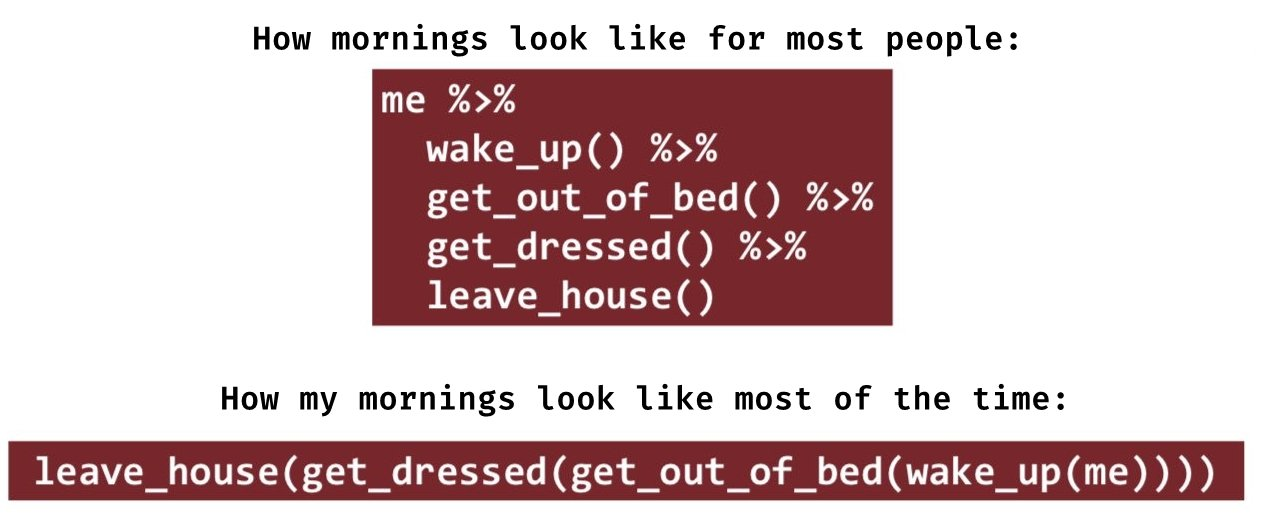
\includegraphics[width=4.16667in,height=\textheight]{images/morning_pipe.png}

В очень редких случаях результат выполнения функции нужно вставить не на
первую позицию (или же мы хотим использовать его несколько раз). В этих
случаях можно использовать \texttt{.}, чтобы обозначить, куда мы хотим
вставить результат выполнения выражения слева от
\texttt{\%\textgreater{}\%}.

\begin{Shaded}
\begin{Highlighting}[]
\StringTok{"Всем привет!"} \SpecialCharTok{\%\textgreater{}\%}
  \FunctionTok{c}\NormalTok{(}\StringTok{"{-}{-}"}\NormalTok{, ., }\StringTok{"{-}{-}"}\NormalTok{)}
\end{Highlighting}
\end{Shaded}

\begin{verbatim}
[1] "--"           "Всем привет!" "--"          
\end{verbatim}

Основные функции в tidyverse \ldots{}

\hypertarget{ux433ux43bux430ux432ux43dux44bux435-ux43fux430ux43aux435ux442ux44b-tidyverse-dplyr-ux438-tidyr}{%
\section{\texorpdfstring{Главные пакеты tidyverse: \texttt{dplyr} и
\texttt{tidyr}}{Главные пакеты tidyverse: dplyr и tidyr}}\label{ux433ux43bux430ux432ux43dux44bux435-ux43fux430ux43aux435ux442ux44b-tidyverse-dplyr-ux438-tidyr}}

\texttt{dplyr}\footnote{\href{https://community.rstudio.com/t/pronunciations-of-common-r-terms/1810}{Есть
  споры о том, как это правильно читать}. Используемые варианты:
  \emph{диплаер}, \emph{диплюр}, \emph{диплир}.} --- это самая основа
всего \texttt{tidyverse}. Этот пакет предоставляет основные функции для
манипуляции с тибблами. Пакет \texttt{dplyr} является наследником и
более усовершенствованной версией \texttt{plyr}, так что если увидите
использование пакета \texttt{plyr}, то, скорее всего, скрипт был написан
очень давно.

Пакет \texttt{tidyr} дополняет \texttt{dplyr}, предоставляя полезные
функции для тайдификации тибблов. Тайдификация (``аккуратизация'')
данных означает приведение табличных данных к такому формату, в котором:

\begin{itemize}
\tightlist
\item
  Каждая переменная имеет собственный столбец
\item
  Каждый наблюдение имеет собственную строку
\item
  Каждое значение имеет свою собственную ячейку
\end{itemize}

Впрочем, многие функции \texttt{dplyr} часто используются при
тайдификации, так же как и многие функции \texttt{tidyr} имеет
применение вне тайдификации. В общем, функционал этих двух пакетов
несколько смешался, поэтому мы будем рассматривать их вместе. А чтобы
представлять, какая функция относится к какому пакету (хотя запоминать
это необязательно), я буду использовать запись с двумя двоеточиями
\texttt{::}, которая обычно используется для использования функции без
подгрузки всего пакета, при первом упоминании функции.

Пакет \texttt{tidyr} --- это более усовершенствованная версия пакета
\texttt{reshape2}, который в свою очередь является усовершенствованной
версией \texttt{reshape}. По аналогии с \texttt{plyr}, если вы видите
использование этих пакетов, то это указывает на то, что перед вами
морально устаревший код.

Код с использованием \texttt{dplyr} и \texttt{tidyr}сильно непохож на
то, что мы видели раньше. Большинство функций \texttt{dplyr} и
\texttt{tidyr} работают с целым тибблом сразу, принимая его в качестве
первого аргумента и возвращая измененный тиббл. Это позволяет превратить
весь код в последовательный набор применяемых функций, соединенный
пайпами. На практике это выглядит очень элегантно, и вы в этом скоро
убедитесь.

\hypertarget{sec-tidy_select_cols}{%
\section{Работа с колонками тиббла}\label{sec-tidy_select_cols}}

\hypertarget{ux432ux44bux431ux43eux440-ux43aux43eux43bux43eux43dux43eux43a-dplyrselect}{%
\subsection{\texorpdfstring{Выбор колонок:
\texttt{dplyr::select()}}{Выбор колонок: dplyr::select()}}\label{ux432ux44bux431ux43eux440-ux43aux43eux43bux43eux43dux43eux43a-dplyrselect}}

Функция \texttt{dplyr::select()} позволяет выбирать колонки по номеру
или имени (кавычки не нужны).

\begin{Shaded}
\begin{Highlighting}[]
\NormalTok{heroes }\SpecialCharTok{\%\textgreater{}\%}
  \FunctionTok{select}\NormalTok{(}\DecValTok{1}\NormalTok{,}\DecValTok{5}\NormalTok{)}
\end{Highlighting}
\end{Shaded}

\begin{verbatim}
# A tibble: 734 x 2
    ...1 Race             
   <dbl> <chr>            
 1     0 Human            
 2     1 Icthyo Sapien    
 3     2 Ungaran          
 4     3 Human / Radiation
 5     4 Cosmic Entity    
 6     5 Human            
 7     6 <NA>             
 8     7 Human            
 9     8 <NA>             
10     9 Human            
# i 724 more rows
\end{verbatim}

\begin{Shaded}
\begin{Highlighting}[]
\NormalTok{heroes }\SpecialCharTok{\%\textgreater{}\%}
  \FunctionTok{select}\NormalTok{(name, Race, Publisher, }\StringTok{\textasciigrave{}}\AttributeTok{Hair color}\StringTok{\textasciigrave{}}\NormalTok{)}
\end{Highlighting}
\end{Shaded}

\begin{verbatim}
# A tibble: 734 x 4
   name          Race              Publisher         `Hair color`
   <chr>         <chr>             <chr>             <chr>       
 1 A-Bomb        Human             Marvel Comics     No Hair     
 2 Abe Sapien    Icthyo Sapien     Dark Horse Comics No Hair     
 3 Abin Sur      Ungaran           DC Comics         No Hair     
 4 Abomination   Human / Radiation Marvel Comics     No Hair     
 5 Abraxas       Cosmic Entity     Marvel Comics     Black       
 6 Absorbing Man Human             Marvel Comics     No Hair     
 7 Adam Monroe   <NA>              NBC - Heroes      Blond       
 8 Adam Strange  Human             DC Comics         Blond       
 9 Agent 13      <NA>              Marvel Comics     Blond       
10 Agent Bob     Human             Marvel Comics     Brown       
# i 724 more rows
\end{verbatim}

Обратите внимание, если в названии колонки присутствует пробел или,
например, колонка начинается с цифры или точки и цифры, то это
синтаксически невалидное имя (@ref(variables)). Это не значит, что такие
названия колонок недопустимы. Но такие названия колонок нужно обособлять
` грависом (правый штрих, на клавиатуре находится там же где и буква ё и
\textasciitilde).

Еще обратите внимание на то, что функции tidyverse не изменяют сами
изначальные тибблы/датафреймы. Это означает, что если вы хотите
полученный результат сохранить, то нужно добавить присвоение:

\begin{Shaded}
\begin{Highlighting}[]
\NormalTok{heroes\_some\_cols }\OtherTok{\textless{}{-}}\NormalTok{ heroes }\SpecialCharTok{\%\textgreater{}\%}
  \FunctionTok{select}\NormalTok{(name, Race, Publisher, }\StringTok{\textasciigrave{}}\AttributeTok{Hair color}\StringTok{\textasciigrave{}}\NormalTok{)}
\NormalTok{heroes\_some\_cols}
\end{Highlighting}
\end{Shaded}

\begin{verbatim}
# A tibble: 734 x 4
   name          Race              Publisher         `Hair color`
   <chr>         <chr>             <chr>             <chr>       
 1 A-Bomb        Human             Marvel Comics     No Hair     
 2 Abe Sapien    Icthyo Sapien     Dark Horse Comics No Hair     
 3 Abin Sur      Ungaran           DC Comics         No Hair     
 4 Abomination   Human / Radiation Marvel Comics     No Hair     
 5 Abraxas       Cosmic Entity     Marvel Comics     Black       
 6 Absorbing Man Human             Marvel Comics     No Hair     
 7 Adam Monroe   <NA>              NBC - Heroes      Blond       
 8 Adam Strange  Human             DC Comics         Blond       
 9 Agent 13      <NA>              Marvel Comics     Blond       
10 Agent Bob     Human             Marvel Comics     Brown       
# i 724 more rows
\end{verbatim}

\hypertarget{sec-tidyselect}{%
\subsection{Мини-язык tidyselect для выбора
колонок}\label{sec-tidyselect}}

Для выбора столбцов (не только в \texttt{select()}, но и для других
функций tidyverse) используется специальный мини-язык tidyselect из
одноименного пакета\footnote{Как и в случае с \texttt{magrittr}, пакет
  \texttt{tidyselect} не содержатся в базовом tidyverse, но функции
  импортируются основыми пакетами tidyverse.}. tidyselect дает очень
широкие возможности для выбора колонок.

Можно использовать оператор \texttt{:} для выбора нескольких соседних
колонок (по аналогии с созданием числового вектора с шагом 1).

\begin{Shaded}
\begin{Highlighting}[]
\NormalTok{heroes }\SpecialCharTok{\%\textgreater{}\%}
  \FunctionTok{select}\NormalTok{(name}\SpecialCharTok{:}\NormalTok{Publisher)}
\end{Highlighting}
\end{Shaded}

\begin{verbatim}
# A tibble: 734 x 7
   name          Gender `Eye color` Race           `Hair color` Height Publisher
   <chr>         <chr>  <chr>       <chr>          <chr>         <dbl> <chr>    
 1 A-Bomb        Male   yellow      Human          No Hair         203 Marvel C~
 2 Abe Sapien    Male   blue        Icthyo Sapien  No Hair         191 Dark Hor~
 3 Abin Sur      Male   blue        Ungaran        No Hair         185 DC Comics
 4 Abomination   Male   green       Human / Radia~ No Hair         203 Marvel C~
 5 Abraxas       Male   blue        Cosmic Entity  Black            NA Marvel C~
 6 Absorbing Man Male   blue        Human          No Hair         193 Marvel C~
 7 Adam Monroe   Male   blue        <NA>           Blond            NA NBC - He~
 8 Adam Strange  Male   blue        Human          Blond           185 DC Comics
 9 Agent 13      Female blue        <NA>           Blond           173 Marvel C~
10 Agent Bob     Male   brown       Human          Brown           178 Marvel C~
# i 724 more rows
\end{verbatim}

\begin{Shaded}
\begin{Highlighting}[]
\NormalTok{heroes }\SpecialCharTok{\%\textgreater{}\%}
  \FunctionTok{select}\NormalTok{(name}\SpecialCharTok{:}\StringTok{\textasciigrave{}}\AttributeTok{Eye color}\StringTok{\textasciigrave{}}\NormalTok{, Publisher}\SpecialCharTok{:}\NormalTok{Weight)}
\end{Highlighting}
\end{Shaded}

\begin{verbatim}
# A tibble: 734 x 7
   name          Gender `Eye color` Publisher      `Skin color` Alignment Weight
   <chr>         <chr>  <chr>       <chr>          <chr>        <chr>      <dbl>
 1 A-Bomb        Male   yellow      Marvel Comics  <NA>         good         441
 2 Abe Sapien    Male   blue        Dark Horse Co~ blue         good          65
 3 Abin Sur      Male   blue        DC Comics      red          good          90
 4 Abomination   Male   green       Marvel Comics  <NA>         bad          441
 5 Abraxas       Male   blue        Marvel Comics  <NA>         bad           NA
 6 Absorbing Man Male   blue        Marvel Comics  <NA>         bad          122
 7 Adam Monroe   Male   blue        NBC - Heroes   <NA>         good          NA
 8 Adam Strange  Male   blue        DC Comics      <NA>         good          88
 9 Agent 13      Female blue        Marvel Comics  <NA>         good          61
10 Agent Bob     Male   brown       Marvel Comics  <NA>         good          81
# i 724 more rows
\end{verbatim}

Используя \texttt{!} можно вырезать ненужные колонки.

\begin{Shaded}
\begin{Highlighting}[]
\NormalTok{heroes }\SpecialCharTok{\%\textgreater{}\%}
  \FunctionTok{select}\NormalTok{(}\SpecialCharTok{!}\NormalTok{...}\DecValTok{1}\NormalTok{)}
\end{Highlighting}
\end{Shaded}

\begin{verbatim}
# A tibble: 734 x 10
   name      Gender `Eye color` Race  `Hair color` Height Publisher `Skin color`
   <chr>     <chr>  <chr>       <chr> <chr>         <dbl> <chr>     <chr>       
 1 A-Bomb    Male   yellow      Human No Hair         203 Marvel C~ <NA>        
 2 Abe Sapi~ Male   blue        Icth~ No Hair         191 Dark Hor~ blue        
 3 Abin Sur  Male   blue        Unga~ No Hair         185 DC Comics red         
 4 Abominat~ Male   green       Huma~ No Hair         203 Marvel C~ <NA>        
 5 Abraxas   Male   blue        Cosm~ Black            NA Marvel C~ <NA>        
 6 Absorbin~ Male   blue        Human No Hair         193 Marvel C~ <NA>        
 7 Adam Mon~ Male   blue        <NA>  Blond            NA NBC - He~ <NA>        
 8 Adam Str~ Male   blue        Human Blond           185 DC Comics <NA>        
 9 Agent 13  Female blue        <NA>  Blond           173 Marvel C~ <NA>        
10 Agent Bob Male   brown       Human Brown           178 Marvel C~ <NA>        
# i 724 more rows
# i 2 more variables: Alignment <chr>, Weight <dbl>
\end{verbatim}

\begin{Shaded}
\begin{Highlighting}[]
\NormalTok{heroes }\SpecialCharTok{\%\textgreater{}\%}
  \FunctionTok{select}\NormalTok{(}\SpecialCharTok{!}\NormalTok{(Gender}\SpecialCharTok{:}\NormalTok{Height))}
\end{Highlighting}
\end{Shaded}

\begin{verbatim}
# A tibble: 734 x 6
    ...1 name          Publisher         `Skin color` Alignment Weight
   <dbl> <chr>         <chr>             <chr>        <chr>      <dbl>
 1     0 A-Bomb        Marvel Comics     <NA>         good         441
 2     1 Abe Sapien    Dark Horse Comics blue         good          65
 3     2 Abin Sur      DC Comics         red          good          90
 4     3 Abomination   Marvel Comics     <NA>         bad          441
 5     4 Abraxas       Marvel Comics     <NA>         bad           NA
 6     5 Absorbing Man Marvel Comics     <NA>         bad          122
 7     6 Adam Monroe   NBC - Heroes      <NA>         good          NA
 8     7 Adam Strange  DC Comics         <NA>         good          88
 9     8 Agent 13      Marvel Comics     <NA>         good          61
10     9 Agent Bob     Marvel Comics     <NA>         good          81
# i 724 more rows
\end{verbatim}

Другие известные нам логические операторы (\texttt{\&} и
\texttt{\textbar{}}) тоже работают в tidyselect.

В дополнение к логическим операторам и \texttt{:}, в tidyselect есть
набор вспомогательных функций, работающих исключительно в контексте
выбора колонок с помощью tidyselect.

Вспомогательная функция \texttt{last\_col()} позволит обратиться к
последней колонке тиббла:

\begin{Shaded}
\begin{Highlighting}[]
\NormalTok{heroes }\SpecialCharTok{\%\textgreater{}\%}
  \FunctionTok{select}\NormalTok{(name}\SpecialCharTok{:}\FunctionTok{last\_col}\NormalTok{())}
\end{Highlighting}
\end{Shaded}

\begin{verbatim}
# A tibble: 734 x 10
   name      Gender `Eye color` Race  `Hair color` Height Publisher `Skin color`
   <chr>     <chr>  <chr>       <chr> <chr>         <dbl> <chr>     <chr>       
 1 A-Bomb    Male   yellow      Human No Hair         203 Marvel C~ <NA>        
 2 Abe Sapi~ Male   blue        Icth~ No Hair         191 Dark Hor~ blue        
 3 Abin Sur  Male   blue        Unga~ No Hair         185 DC Comics red         
 4 Abominat~ Male   green       Huma~ No Hair         203 Marvel C~ <NA>        
 5 Abraxas   Male   blue        Cosm~ Black            NA Marvel C~ <NA>        
 6 Absorbin~ Male   blue        Human No Hair         193 Marvel C~ <NA>        
 7 Adam Mon~ Male   blue        <NA>  Blond            NA NBC - He~ <NA>        
 8 Adam Str~ Male   blue        Human Blond           185 DC Comics <NA>        
 9 Agent 13  Female blue        <NA>  Blond           173 Marvel C~ <NA>        
10 Agent Bob Male   brown       Human Brown           178 Marvel C~ <NA>        
# i 724 more rows
# i 2 more variables: Alignment <chr>, Weight <dbl>
\end{verbatim}

А функция \texttt{everything()} позволяет выбрать все колонки.

\begin{Shaded}
\begin{Highlighting}[]
\NormalTok{heroes }\SpecialCharTok{\%\textgreater{}\%}
  \FunctionTok{select}\NormalTok{(}\FunctionTok{everything}\NormalTok{())}
\end{Highlighting}
\end{Shaded}

\begin{verbatim}
# A tibble: 734 x 11
    ...1 name          Gender `Eye color` Race     `Hair color` Height Publisher
   <dbl> <chr>         <chr>  <chr>       <chr>    <chr>         <dbl> <chr>    
 1     0 A-Bomb        Male   yellow      Human    No Hair         203 Marvel C~
 2     1 Abe Sapien    Male   blue        Icthyo ~ No Hair         191 Dark Hor~
 3     2 Abin Sur      Male   blue        Ungaran  No Hair         185 DC Comics
 4     3 Abomination   Male   green       Human /~ No Hair         203 Marvel C~
 5     4 Abraxas       Male   blue        Cosmic ~ Black            NA Marvel C~
 6     5 Absorbing Man Male   blue        Human    No Hair         193 Marvel C~
 7     6 Adam Monroe   Male   blue        <NA>     Blond            NA NBC - He~
 8     7 Adam Strange  Male   blue        Human    Blond           185 DC Comics
 9     8 Agent 13      Female blue        <NA>     Blond           173 Marvel C~
10     9 Agent Bob     Male   brown       Human    Brown           178 Marvel C~
# i 724 more rows
# i 3 more variables: `Skin color` <chr>, Alignment <chr>, Weight <dbl>
\end{verbatim}

При этом \texttt{everything()} не будет дублировать выбранные колонки,
поэтому можно использовать \texttt{everything()} для перестановки
колонок в тиббле:

\begin{Shaded}
\begin{Highlighting}[]
\NormalTok{heroes }\SpecialCharTok{\%\textgreater{}\%}
  \FunctionTok{select}\NormalTok{(name, Publisher, }\FunctionTok{everything}\NormalTok{())}
\end{Highlighting}
\end{Shaded}

\begin{verbatim}
# A tibble: 734 x 11
   name          Publisher     ...1 Gender `Eye color` Race  `Hair color` Height
   <chr>         <chr>        <dbl> <chr>  <chr>       <chr> <chr>         <dbl>
 1 A-Bomb        Marvel Comi~     0 Male   yellow      Human No Hair         203
 2 Abe Sapien    Dark Horse ~     1 Male   blue        Icth~ No Hair         191
 3 Abin Sur      DC Comics        2 Male   blue        Unga~ No Hair         185
 4 Abomination   Marvel Comi~     3 Male   green       Huma~ No Hair         203
 5 Abraxas       Marvel Comi~     4 Male   blue        Cosm~ Black            NA
 6 Absorbing Man Marvel Comi~     5 Male   blue        Human No Hair         193
 7 Adam Monroe   NBC - Heroes     6 Male   blue        <NA>  Blond            NA
 8 Adam Strange  DC Comics        7 Male   blue        Human Blond           185
 9 Agent 13      Marvel Comi~     8 Female blue        <NA>  Blond           173
10 Agent Bob     Marvel Comi~     9 Male   brown       Human Brown           178
# i 724 more rows
# i 3 more variables: `Skin color` <chr>, Alignment <chr>, Weight <dbl>
\end{verbatim}

Впрочем, для перестановки колонок удобнее использовать специальную
функцию \texttt{relocate()} (@ref(tidy\_relocate)) Можно даже выбирать
колонки по паттернам в названиях. Например, с помощью
\texttt{ends\_with()} можно выбрать все колонки, заканчивающиеся
одинаковым суффиксом:

\begin{Shaded}
\begin{Highlighting}[]
\NormalTok{heroes }\SpecialCharTok{\%\textgreater{}\%}
  \FunctionTok{select}\NormalTok{(}\FunctionTok{ends\_with}\NormalTok{(}\StringTok{"color"}\NormalTok{))}
\end{Highlighting}
\end{Shaded}

\begin{verbatim}
# A tibble: 734 x 3
   `Eye color` `Hair color` `Skin color`
   <chr>       <chr>        <chr>       
 1 yellow      No Hair      <NA>        
 2 blue        No Hair      blue        
 3 blue        No Hair      red         
 4 green       No Hair      <NA>        
 5 blue        Black        <NA>        
 6 blue        No Hair      <NA>        
 7 blue        Blond        <NA>        
 8 blue        Blond        <NA>        
 9 blue        Blond        <NA>        
10 brown       Brown        <NA>        
# i 724 more rows
\end{verbatim}

Аналогично, с помощью функции \texttt{starts\_with()} можно найти
колонки с одинаковым префиксом, с помощью \texttt{contains()} --- все
колонки с выбранным паттерном в любой части названия колонки\footnote{Выбранный
  паттерн будет найден посимвольно, если же вы хотите искать по
  регулярным выражениям, то вместо \texttt{contains()} нужно
  использовать \texttt{matches()}.}.

\begin{Shaded}
\begin{Highlighting}[]
\NormalTok{heroes }\SpecialCharTok{\%\textgreater{}\%}
  \FunctionTok{select}\NormalTok{(}\FunctionTok{starts\_with}\NormalTok{(}\StringTok{"Eye"}\NormalTok{) }\SpecialCharTok{\&} \FunctionTok{ends\_with}\NormalTok{(}\StringTok{"color"}\NormalTok{))}
\end{Highlighting}
\end{Shaded}

\begin{verbatim}
# A tibble: 734 x 1
   `Eye color`
   <chr>      
 1 yellow     
 2 blue       
 3 blue       
 4 green      
 5 blue       
 6 blue       
 7 blue       
 8 blue       
 9 blue       
10 brown      
# i 724 more rows
\end{verbatim}

\begin{Shaded}
\begin{Highlighting}[]
\NormalTok{heroes }\SpecialCharTok{\%\textgreater{}\%}
  \FunctionTok{select}\NormalTok{(}\FunctionTok{contains}\NormalTok{(}\StringTok{"eight"}\NormalTok{))}
\end{Highlighting}
\end{Shaded}

\begin{verbatim}
# A tibble: 734 x 2
   Height Weight
    <dbl>  <dbl>
 1    203    441
 2    191     65
 3    185     90
 4    203    441
 5     NA     NA
 6    193    122
 7     NA     NA
 8    185     88
 9    173     61
10    178     81
# i 724 more rows
\end{verbatim}

Ну и наконец, можно выбирать по содержимому колонок с помощью
\texttt{where()}. Это напоминает применение
\texttt{sapply()}(@ref(apply\_other)) на датафрейме для индексирования
колонок: в качестве аргумента для \texttt{where} принимается функция,
которая применяется для каждой из колонок, после чего выбираются только
те колонки, для которых было получено \texttt{TRUE}.

\begin{Shaded}
\begin{Highlighting}[]
\NormalTok{heroes }\SpecialCharTok{\%\textgreater{}\%}
  \FunctionTok{select}\NormalTok{(}\FunctionTok{where}\NormalTok{(is.numeric))}
\end{Highlighting}
\end{Shaded}

\begin{verbatim}
# A tibble: 734 x 3
    ...1 Height Weight
   <dbl>  <dbl>  <dbl>
 1     0    203    441
 2     1    191     65
 3     2    185     90
 4     3    203    441
 5     4     NA     NA
 6     5    193    122
 7     6     NA     NA
 8     7    185     88
 9     8    173     61
10     9    178     81
# i 724 more rows
\end{verbatim}

Функция \texttt{where()} дает невиданную мощь. Например, можно выбрать
все колонки без \texttt{NA}:

\begin{Shaded}
\begin{Highlighting}[]
\NormalTok{heroes }\SpecialCharTok{\%\textgreater{}\%}
  \FunctionTok{select}\NormalTok{(}\FunctionTok{where}\NormalTok{(}\ControlFlowTok{function}\NormalTok{(x) }\SpecialCharTok{!}\FunctionTok{any}\NormalTok{(}\FunctionTok{is.na}\NormalTok{(x))))}
\end{Highlighting}
\end{Shaded}

\begin{verbatim}
# A tibble: 734 x 3
    ...1 name          Publisher        
   <dbl> <chr>         <chr>            
 1     0 A-Bomb        Marvel Comics    
 2     1 Abe Sapien    Dark Horse Comics
 3     2 Abin Sur      DC Comics        
 4     3 Abomination   Marvel Comics    
 5     4 Abraxas       Marvel Comics    
 6     5 Absorbing Man Marvel Comics    
 7     6 Adam Monroe   NBC - Heroes     
 8     7 Adam Strange  DC Comics        
 9     8 Agent 13      Marvel Comics    
10     9 Agent Bob     Marvel Comics    
# i 724 more rows
\end{verbatim}

\#\#\#Переименование колонок: \texttt{dplyr::rename()}

Внутри \texttt{select()} можно не только выбирать колонки, но и
переименовывать их:

\begin{Shaded}
\begin{Highlighting}[]
\NormalTok{heroes }\SpecialCharTok{\%\textgreater{}\%}
  \FunctionTok{select}\NormalTok{(}\AttributeTok{id =}\NormalTok{ ...}\DecValTok{1}\NormalTok{)}
\end{Highlighting}
\end{Shaded}

\begin{verbatim}
# A tibble: 734 x 1
      id
   <dbl>
 1     0
 2     1
 3     2
 4     3
 5     4
 6     5
 7     6
 8     7
 9     8
10     9
# i 724 more rows
\end{verbatim}

Однако удобнее для этого использовать специальную функцию
\texttt{dplyr::rename()}. Синтаксис у нее такой же, как и у
\texttt{select()}, но \texttt{rename()} не выбрасывает колонки, которые
не были упомянуты.

\begin{Shaded}
\begin{Highlighting}[]
\NormalTok{heroes }\SpecialCharTok{\%\textgreater{}\%}
  \FunctionTok{rename}\NormalTok{(}\AttributeTok{id =}\NormalTok{ ...}\DecValTok{1}\NormalTok{)}
\end{Highlighting}
\end{Shaded}

\begin{verbatim}
# A tibble: 734 x 11
      id name          Gender `Eye color` Race     `Hair color` Height Publisher
   <dbl> <chr>         <chr>  <chr>       <chr>    <chr>         <dbl> <chr>    
 1     0 A-Bomb        Male   yellow      Human    No Hair         203 Marvel C~
 2     1 Abe Sapien    Male   blue        Icthyo ~ No Hair         191 Dark Hor~
 3     2 Abin Sur      Male   blue        Ungaran  No Hair         185 DC Comics
 4     3 Abomination   Male   green       Human /~ No Hair         203 Marvel C~
 5     4 Abraxas       Male   blue        Cosmic ~ Black            NA Marvel C~
 6     5 Absorbing Man Male   blue        Human    No Hair         193 Marvel C~
 7     6 Adam Monroe   Male   blue        <NA>     Blond            NA NBC - He~
 8     7 Adam Strange  Male   blue        Human    Blond           185 DC Comics
 9     8 Agent 13      Female blue        <NA>     Blond           173 Marvel C~
10     9 Agent Bob     Male   brown       Human    Brown           178 Marvel C~
# i 724 more rows
# i 3 more variables: `Skin color` <chr>, Alignment <chr>, Weight <dbl>
\end{verbatim}

Для массового переименования колонок можно использовать функцию
\texttt{rename\_with()}. Эта функция так же использует tidyselect
синтаксис для выбора колонок (по умолчанию выбираются все колонки) и
применяет функцию в качестве аргумента, которая изменяет

\begin{Shaded}
\begin{Highlighting}[]
\NormalTok{heroes }\SpecialCharTok{\%\textgreater{}\%}
  \FunctionTok{rename\_with}\NormalTok{(make.names)}
\end{Highlighting}
\end{Shaded}

\begin{verbatim}
# A tibble: 734 x 11
    ...1 name      Gender Eye.color Race  Hair.color Height Publisher Skin.color
   <dbl> <chr>     <chr>  <chr>     <chr> <chr>       <dbl> <chr>     <chr>     
 1     0 A-Bomb    Male   yellow    Human No Hair       203 Marvel C~ <NA>      
 2     1 Abe Sapi~ Male   blue      Icth~ No Hair       191 Dark Hor~ blue      
 3     2 Abin Sur  Male   blue      Unga~ No Hair       185 DC Comics red       
 4     3 Abominat~ Male   green     Huma~ No Hair       203 Marvel C~ <NA>      
 5     4 Abraxas   Male   blue      Cosm~ Black          NA Marvel C~ <NA>      
 6     5 Absorbin~ Male   blue      Human No Hair       193 Marvel C~ <NA>      
 7     6 Adam Mon~ Male   blue      <NA>  Blond          NA NBC - He~ <NA>      
 8     7 Adam Str~ Male   blue      Human Blond         185 DC Comics <NA>      
 9     8 Agent 13  Female blue      <NA>  Blond         173 Marvel C~ <NA>      
10     9 Agent Bob Male   brown     Human Brown         178 Marvel C~ <NA>      
# i 724 more rows
# i 2 more variables: Alignment <chr>, Weight <dbl>
\end{verbatim}

\#\#\#Перестановка колонок: \texttt{dplyr::relocate()}
\{\#sec-tidy\_relocate\}

Для изменения порядка колонок можно использовать функцию
\texttt{relocate()}. Она тоже работает похожим образом на
\texttt{select()} и \texttt{rename()}\footnote{\texttt{relocate()} не
  позволяет переименовывать колонки в отличие от \texttt{select()} и
  \texttt{rename()}}. Как и \texttt{rename()}, функция
\texttt{relocate()} не выкидывает неиспользованные колонки:

\begin{Shaded}
\begin{Highlighting}[]
\NormalTok{heroes }\SpecialCharTok{\%\textgreater{}\%}
  \FunctionTok{relocate}\NormalTok{(Publisher)}
\end{Highlighting}
\end{Shaded}

\begin{verbatim}
# A tibble: 734 x 11
   Publisher          ...1 name     Gender `Eye color` Race  `Hair color` Height
   <chr>             <dbl> <chr>    <chr>  <chr>       <chr> <chr>         <dbl>
 1 Marvel Comics         0 A-Bomb   Male   yellow      Human No Hair         203
 2 Dark Horse Comics     1 Abe Sap~ Male   blue        Icth~ No Hair         191
 3 DC Comics             2 Abin Sur Male   blue        Unga~ No Hair         185
 4 Marvel Comics         3 Abomina~ Male   green       Huma~ No Hair         203
 5 Marvel Comics         4 Abraxas  Male   blue        Cosm~ Black            NA
 6 Marvel Comics         5 Absorbi~ Male   blue        Human No Hair         193
 7 NBC - Heroes          6 Adam Mo~ Male   blue        <NA>  Blond            NA
 8 DC Comics             7 Adam St~ Male   blue        Human Blond           185
 9 Marvel Comics         8 Agent 13 Female blue        <NA>  Blond           173
10 Marvel Comics         9 Agent B~ Male   brown       Human Brown           178
# i 724 more rows
# i 3 more variables: `Skin color` <chr>, Alignment <chr>, Weight <dbl>
\end{verbatim}

При этом \texttt{relocate()} имеет дополнительные параметры
\texttt{.after\ =} и \texttt{.before\ =}, которые позволяют выбирать,
куда поместить выбранные колонки.

\begin{Shaded}
\begin{Highlighting}[]
\NormalTok{heroes }\SpecialCharTok{\%\textgreater{}\%}
  \FunctionTok{relocate}\NormalTok{(Publisher, }\AttributeTok{.after =}\NormalTok{ name)}
\end{Highlighting}
\end{Shaded}

\begin{verbatim}
# A tibble: 734 x 11
    ...1 name          Publisher    Gender `Eye color` Race  `Hair color` Height
   <dbl> <chr>         <chr>        <chr>  <chr>       <chr> <chr>         <dbl>
 1     0 A-Bomb        Marvel Comi~ Male   yellow      Human No Hair         203
 2     1 Abe Sapien    Dark Horse ~ Male   blue        Icth~ No Hair         191
 3     2 Abin Sur      DC Comics    Male   blue        Unga~ No Hair         185
 4     3 Abomination   Marvel Comi~ Male   green       Huma~ No Hair         203
 5     4 Abraxas       Marvel Comi~ Male   blue        Cosm~ Black            NA
 6     5 Absorbing Man Marvel Comi~ Male   blue        Human No Hair         193
 7     6 Adam Monroe   NBC - Heroes Male   blue        <NA>  Blond            NA
 8     7 Adam Strange  DC Comics    Male   blue        Human Blond           185
 9     8 Agent 13      Marvel Comi~ Female blue        <NA>  Blond           173
10     9 Agent Bob     Marvel Comi~ Male   brown       Human Brown           178
# i 724 more rows
# i 3 more variables: `Skin color` <chr>, Alignment <chr>, Weight <dbl>
\end{verbatim}

\texttt{relocate()} очень хорошо работает в сочетании с выбором колонок
с помощью tidyselect. Например, можно передвинуть в одно место все
колонки с одним типом данных:

\begin{Shaded}
\begin{Highlighting}[]
\NormalTok{heroes }\SpecialCharTok{\%\textgreater{}\%}
  \FunctionTok{relocate}\NormalTok{(Publisher, }\FunctionTok{where}\NormalTok{(is.numeric), }\AttributeTok{.after =}\NormalTok{ name)}
\end{Highlighting}
\end{Shaded}

\begin{verbatim}
# A tibble: 734 x 11
   name      Publisher  ...1 Height Weight Gender `Eye color` Race  `Hair color`
   <chr>     <chr>     <dbl>  <dbl>  <dbl> <chr>  <chr>       <chr> <chr>       
 1 A-Bomb    Marvel C~     0    203    441 Male   yellow      Human No Hair     
 2 Abe Sapi~ Dark Hor~     1    191     65 Male   blue        Icth~ No Hair     
 3 Abin Sur  DC Comics     2    185     90 Male   blue        Unga~ No Hair     
 4 Abominat~ Marvel C~     3    203    441 Male   green       Huma~ No Hair     
 5 Abraxas   Marvel C~     4     NA     NA Male   blue        Cosm~ Black       
 6 Absorbin~ Marvel C~     5    193    122 Male   blue        Human No Hair     
 7 Adam Mon~ NBC - He~     6     NA     NA Male   blue        <NA>  Blond       
 8 Adam Str~ DC Comics     7    185     88 Male   blue        Human Blond       
 9 Agent 13  Marvel C~     8    173     61 Female blue        <NA>  Blond       
10 Agent Bob Marvel C~     9    178     81 Male   brown       Human Brown       
# i 724 more rows
# i 2 more variables: `Skin color` <chr>, Alignment <chr>
\end{verbatim}

Последняя важная функция для выбора колонок --- \texttt{pull()}. Эта
функция делает то же самое, что и индексирование с помощью \texttt{\$},
т.е. вытаскивает из тиббла вектор с выбранным названием. Это лучше
вписывается в логику tidyverse, поскольку позволяет извлечь колонку из
тиббла с использованием пайпа:

\begin{Shaded}
\begin{Highlighting}[]
\NormalTok{heroes }\SpecialCharTok{\%\textgreater{}\%}
  \FunctionTok{select}\NormalTok{(Height) }\SpecialCharTok{\%\textgreater{}\%}
  \FunctionTok{pull}\NormalTok{() }\SpecialCharTok{\%\textgreater{}\%}
  \FunctionTok{head}\NormalTok{()}
\end{Highlighting}
\end{Shaded}

\begin{verbatim}
[1] 203 191 185 203  NA 193
\end{verbatim}

\begin{Shaded}
\begin{Highlighting}[]
\NormalTok{heroes }\SpecialCharTok{\%\textgreater{}\%}
  \FunctionTok{pull}\NormalTok{(Height) }\SpecialCharTok{\%\textgreater{}\%}
  \FunctionTok{head}\NormalTok{()}
\end{Highlighting}
\end{Shaded}

\begin{verbatim}
[1] 203 191 185 203  NA 193
\end{verbatim}

У функции \texttt{pull()} есть аргумент \texttt{name\ =}, который
позволяет создать проименованный вектор:

\begin{Shaded}
\begin{Highlighting}[]
\NormalTok{heroes }\SpecialCharTok{\%\textgreater{}\%}
  \FunctionTok{pull}\NormalTok{(Height, name) }\SpecialCharTok{\%\textgreater{}\%}
  \FunctionTok{head}\NormalTok{()}
\end{Highlighting}
\end{Shaded}

\begin{verbatim}
       A-Bomb    Abe Sapien      Abin Sur   Abomination       Abraxas 
          203           191           185           203            NA 
Absorbing Man 
          193 
\end{verbatim}

В отличие от базового R, tidyverse нигде не сокращает имплицитно
результат вычислений до вектора, поэтому функция \texttt{pull()} - это
основной способ извлечения колонки из тиббла как вектора.

\hypertarget{sec-tidy_select_rows}{%
\section{Работа со строками тиббла}\label{sec-tidy_select_rows}}

\hypertarget{sec-tidy_slice}{%
\subsection{\texorpdfstring{Выбор строк по номеру:
\texttt{dplyr::slice()}}{Выбор строк по номеру: dplyr::slice()}}\label{sec-tidy_slice}}

Начнем с выбора строк. Функция \texttt{dplyr::slice()} выбирает строчки
по их числовому индексу.

\begin{Shaded}
\begin{Highlighting}[]
\NormalTok{heroes }\SpecialCharTok{\%\textgreater{}\%}
  \FunctionTok{slice}\NormalTok{(}\DecValTok{1}\SpecialCharTok{:}\DecValTok{3}\NormalTok{)}
\end{Highlighting}
\end{Shaded}

\begin{verbatim}
# A tibble: 3 x 11
   ...1 name       Gender `Eye color` Race         `Hair color` Height Publisher
  <dbl> <chr>      <chr>  <chr>       <chr>        <chr>         <dbl> <chr>    
1     0 A-Bomb     Male   yellow      Human        No Hair         203 Marvel C~
2     1 Abe Sapien Male   blue        Icthyo Sapi~ No Hair         191 Dark Hor~
3     2 Abin Sur   Male   blue        Ungaran      No Hair         185 DC Comics
# i 3 more variables: `Skin color` <chr>, Alignment <chr>, Weight <dbl>
\end{verbatim}

\hypertarget{sec-tidy_filter}{%
\subsection{\texorpdfstring{Выбор строк по условию:
\texttt{dplyr::filter()}}{Выбор строк по условию: dplyr::filter()}}\label{sec-tidy_filter}}

Функция \texttt{dplyr::filter()} делает то же самое, что и
\texttt{slice()}, но уже по условию. Причем для условий нужно
использовать не векторы из тиббла, а название колонок (без кавычек) как
будто бы они были переменными в окружении.

\begin{Shaded}
\begin{Highlighting}[]
\NormalTok{heroes }\SpecialCharTok{\%\textgreater{}\%} 
  \FunctionTok{filter}\NormalTok{(Publisher }\SpecialCharTok{==} \StringTok{"DC Comics"}\NormalTok{)}
\end{Highlighting}
\end{Shaded}

\begin{verbatim}
# A tibble: 215 x 11
    ...1 name             Gender `Eye color` Race  `Hair color` Height Publisher
   <dbl> <chr>            <chr>  <chr>       <chr> <chr>         <dbl> <chr>    
 1     2 Abin Sur         Male   blue        Unga~ No Hair         185 DC Comics
 2     7 Adam Strange     Male   blue        Human Blond           185 DC Comics
 3    13 Alan Scott       Male   blue        <NA>  Blond           180 DC Comics
 4    16 Alfred Pennywor~ Male   blue        Human Black           178 DC Comics
 5    19 Amazo            Male   red         Andr~ <NA>            257 DC Comics
 6    27 Animal Man       Male   blue        Human Blond           183 DC Comics
 7    31 Anti-Monitor     Male   yellow      God ~ No Hair          61 DC Comics
 8    35 Aquababy         Male   blue        <NA>  Blond            NA DC Comics
 9    36 Aqualad          Male   blue        Atla~ Black           178 DC Comics
10    37 Aquaman          Male   blue        Atla~ Blond           185 DC Comics
# i 205 more rows
# i 3 more variables: `Skin color` <chr>, Alignment <chr>, Weight <dbl>
\end{verbatim}

\hypertarget{sec-slice_family}{%
\subsection{\texorpdfstring{Семейство функций
\texttt{slice()}}{Семейство функций slice()}}\label{sec-slice_family}}

У функции \texttt{slice()} есть множество родственников, которые
объединяют функционал обычного \texttt{slice()} и \texttt{filter()}.
Например, с помощью функций \texttt{dplyr::slice\_max()} и
\texttt{dplyr::slice\_min()} можно выбрать заданное количество строк,
содержащих наибольшие или наименьшие значения по колонке соответственно:

\begin{Shaded}
\begin{Highlighting}[]
\NormalTok{heroes }\SpecialCharTok{\%\textgreater{}\%}
  \FunctionTok{slice\_max}\NormalTok{(Weight, }\AttributeTok{n =} \DecValTok{3}\NormalTok{)}
\end{Highlighting}
\end{Shaded}

\begin{verbatim}
# A tibble: 3 x 11
   ...1 name       Gender `Eye color` Race    `Hair color` Height Publisher    
  <dbl> <chr>      <chr>  <chr>       <chr>   <chr>         <dbl> <chr>        
1   575 Sasquatch  Male   red         <NA>    Orange          305 Marvel Comics
2   373 Juggernaut Male   blue        Human   Red             287 Marvel Comics
3   203 Darkseid   Male   red         New God No Hair         267 DC Comics    
# i 3 more variables: `Skin color` <chr>, Alignment <chr>, Weight <dbl>
\end{verbatim}

\begin{Shaded}
\begin{Highlighting}[]
\NormalTok{heroes }\SpecialCharTok{\%\textgreater{}\%}
  \FunctionTok{slice\_min}\NormalTok{(Weight, }\AttributeTok{n =} \DecValTok{3}\NormalTok{)}
\end{Highlighting}
\end{Shaded}

\begin{verbatim}
# A tibble: 3 x 11
   ...1 name        Gender `Eye color` Race        `Hair color` Height Publisher
  <dbl> <chr>       <chr>  <chr>       <chr>       <chr>         <dbl> <chr>    
1   346 Iron Monger Male   blue        <NA>        No Hair          NA Marvel C~
2   302 Groot       Male   yellow      Flora Colo~ <NA>            701 Marvel C~
3   350 Jack-Jack   Male   blue        Human       Brown            71 Dark Hor~
# i 3 more variables: `Skin color` <chr>, Alignment <chr>, Weight <dbl>
\end{verbatim}

Функция \texttt{slice\_sample()} позволяет выбирать заданное количество
случайных строчек:

\begin{Shaded}
\begin{Highlighting}[]
\NormalTok{heroes }\SpecialCharTok{\%\textgreater{}\%}
  \FunctionTok{slice\_sample}\NormalTok{(}\AttributeTok{n =} \DecValTok{3}\NormalTok{)}
\end{Highlighting}
\end{Shaded}

\begin{verbatim}
# A tibble: 3 x 11
   ...1 name     Gender `Eye color` Race     `Hair color` Height Publisher    
  <dbl> <chr>    <chr>  <chr>       <chr>    <chr>         <dbl> <chr>        
1   324 Hercules Male   blue        Demi-God Brown           196 Marvel Comics
2   425 Magus    Male   black       <NA>     <NA>            183 Marvel Comics
3   345 Iron Man Male   blue        Human    Black           198 Marvel Comics
# i 3 more variables: `Skin color` <chr>, Alignment <chr>, Weight <dbl>
\end{verbatim}

Или же долю строчек:

\begin{Shaded}
\begin{Highlighting}[]
\NormalTok{heroes }\SpecialCharTok{\%\textgreater{}\%}
  \FunctionTok{slice\_sample}\NormalTok{(}\AttributeTok{prop =}\NormalTok{ .}\DecValTok{01}\NormalTok{)}
\end{Highlighting}
\end{Shaded}

\begin{verbatim}
# A tibble: 7 x 11
   ...1 name          Gender `Eye color` Race      `Hair color` Height Publisher
  <dbl> <chr>         <chr>  <chr>       <chr>     <chr>         <dbl> <chr>    
1   146 Cameron Hicks Male   <NA>        Alpha     <NA>             NA SyFy     
2    60 Banshee       Male   green       Human     Strawberry ~    183 Marvel C~
3   443 Mephisto      Male   white       <NA>      Black           198 Marvel C~
4   315 Hawkman       Male   blue        <NA>      Brown           185 DC Comics
5   186 Corsair       Male   brown       <NA>      Brown           191 Marvel C~
6   469 Monica Dawson Female <NA>        <NA>      <NA>             NA NBC - He~
7   388 Kilowog       Male   red         Bolovaxi~ No Hair         234 DC Comics
# i 3 more variables: `Skin color` <chr>, Alignment <chr>, Weight <dbl>
\end{verbatim}

Если поставить значение параметра \texttt{prop\ =} равным \texttt{1}, то
таким образом можно перемешать порядок строчек в тиббле:

\begin{Shaded}
\begin{Highlighting}[]
\NormalTok{heroes }\SpecialCharTok{\%\textgreater{}\%}
  \FunctionTok{slice\_sample}\NormalTok{(}\AttributeTok{prop =} \DecValTok{1}\NormalTok{)}
\end{Highlighting}
\end{Shaded}

\begin{verbatim}
# A tibble: 734 x 11
    ...1 name             Gender `Eye color` Race  `Hair color` Height Publisher
   <dbl> <chr>            <chr>  <chr>       <chr> <chr>         <dbl> <chr>    
 1   463 MODOK            Male   white       Cybo~ Brownn          366 Marvel C~
 2     7 Adam Strange     Male   blue        Human Blond           185 DC Comics
 3   162 Cat              Female blue        <NA>  Blond           173 Marvel C~
 4   492 Niki Sanders     Female blue        <NA>  Blond            NA NBC - He~
 5   291 Goliath          Male   <NA>        Human <NA>             NA Marvel C~
 6   221 Doctor Doom      Male   brown       Human Brown           201 Marvel C~
 7   268 Franklin Richar~ Male   blue        Muta~ Blond           142 Marvel C~
 8   101 Black Knight III Male   brown       Human Brown           183 Marvel C~
 9   691 Venom III        Male   brown       Symb~ Brown           229 Marvel C~
10   672 Toad             Male   black       Muta~ Brown           175 Marvel C~
# i 724 more rows
# i 3 more variables: `Skin color` <chr>, Alignment <chr>, Weight <dbl>
\end{verbatim}

\hypertarget{sec-tidy_drop_na}{%
\subsection{\texorpdfstring{Удаление строчек с NA:
\texttt{tidyr::drop\_na()}}{Удаление строчек с NA: tidyr::drop\_na()}}\label{sec-tidy_drop_na}}

Если нужно выбрать только строчки без пропущенных значений, то можно
воспользоваться удобной функцией \texttt{tidyr::drop\_na()}.

\begin{Shaded}
\begin{Highlighting}[]
\NormalTok{heroes }\SpecialCharTok{\%\textgreater{}\%}
  \FunctionTok{drop\_na}\NormalTok{()}
\end{Highlighting}
\end{Shaded}

\begin{verbatim}
# A tibble: 50 x 11
    ...1 name       Gender `Eye color` Race        `Hair color` Height Publisher
   <dbl> <chr>      <chr>  <chr>       <chr>       <chr>         <dbl> <chr>    
 1     1 Abe Sapien Male   blue        Icthyo Sap~ No Hair         191 Dark Hor~
 2     2 Abin Sur   Male   blue        Ungaran     No Hair         185 DC Comics
 3    34 Apocalypse Male   red         Mutant      Black           213 Marvel C~
 4    39 Archangel  Male   blue        Mutant      Blond           183 Marvel C~
 5    41 Ardina     Female white       Alien       Orange          193 Marvel C~
 6    56 Azazel     Male   yellow      Neyaphem    Black           183 Marvel C~
 7    74 Beast      Male   blue        Mutant      Blue            180 Marvel C~
 8    75 Beast Boy  Male   green       Human       Green           173 DC Comics
 9    92 Bizarro    Male   black       Bizarro     Black           191 DC Comics
10   108 Blackout   Male   red         Demon       White           191 Marvel C~
# i 40 more rows
# i 3 more variables: `Skin color` <chr>, Alignment <chr>, Weight <dbl>
\end{verbatim}

Можно выбрать колонки, наличие \texttt{NA} в которых будет приводить к
удалению соответствующих строчек (не затрагивая другие строчки, в
которых есть \texttt{NA} в остальных столбцах).

\begin{Shaded}
\begin{Highlighting}[]
\NormalTok{heroes }\SpecialCharTok{\%\textgreater{}\%}
  \FunctionTok{drop\_na}\NormalTok{(Weight)}
\end{Highlighting}
\end{Shaded}

\begin{verbatim}
# A tibble: 495 x 11
    ...1 name          Gender `Eye color` Race     `Hair color` Height Publisher
   <dbl> <chr>         <chr>  <chr>       <chr>    <chr>         <dbl> <chr>    
 1     0 A-Bomb        Male   yellow      Human    No Hair         203 Marvel C~
 2     1 Abe Sapien    Male   blue        Icthyo ~ No Hair         191 Dark Hor~
 3     2 Abin Sur      Male   blue        Ungaran  No Hair         185 DC Comics
 4     3 Abomination   Male   green       Human /~ No Hair         203 Marvel C~
 5     5 Absorbing Man Male   blue        Human    No Hair         193 Marvel C~
 6     7 Adam Strange  Male   blue        Human    Blond           185 DC Comics
 7     8 Agent 13      Female blue        <NA>     Blond           173 Marvel C~
 8     9 Agent Bob     Male   brown       Human    Brown           178 Marvel C~
 9    10 Agent Zero    Male   <NA>        <NA>     <NA>            191 Marvel C~
10    11 Air-Walker    Male   blue        <NA>     White           188 Marvel C~
# i 485 more rows
# i 3 more variables: `Skin color` <chr>, Alignment <chr>, Weight <dbl>
\end{verbatim}

Для выбора колонок в \texttt{drop\_na()} используется tidyselect, с
которым мы недавно познакомились (@ref(tidyselect)).

\hypertarget{sec-tidy_arrange}{%
\subsection{\texorpdfstring{Сортировка строк:
\texttt{dplyr::arrange()}}{Сортировка строк: dplyr::arrange()}}\label{sec-tidy_arrange}}

Функция \texttt{dplyr::arrange()} сортирует строчки от меньшего к
большему (или по алфавиту - для текстовых значений) по выбранной
колонке.

\begin{Shaded}
\begin{Highlighting}[]
\NormalTok{heroes }\SpecialCharTok{\%\textgreater{}\%}
  \FunctionTok{arrange}\NormalTok{(Weight)}
\end{Highlighting}
\end{Shaded}

\begin{verbatim}
# A tibble: 734 x 11
    ...1 name            Gender `Eye color` Race   `Hair color` Height Publisher
   <dbl> <chr>           <chr>  <chr>       <chr>  <chr>         <dbl> <chr>    
 1   346 Iron Monger     Male   blue        <NA>   No Hair          NA Marvel C~
 2   302 Groot           Male   yellow      Flora~ <NA>            701 Marvel C~
 3   350 Jack-Jack       Male   blue        Human  Brown            71 Dark Hor~
 4   272 Galactus        Male   black       Cosmi~ Black           876 Marvel C~
 5   731 Yoda            Male   brown       Yoda'~ White            66 George L~
 6   255 Fin Fang Foom   Male   red         Kakar~ No Hair         975 Marvel C~
 7   330 Howard the Duck Male   brown       <NA>   Yellow           79 Marvel C~
 8   396 Krypto          Male   blue        Krypt~ White            64 DC Comics
 9   568 Rocket Raccoon  Male   brown       Animal Brown           122 Marvel C~
10   208 Dash            Male   blue        Human  Blond           122 Dark Hor~
# i 724 more rows
# i 3 more variables: `Skin color` <chr>, Alignment <chr>, Weight <dbl>
\end{verbatim}

Чтобы отсортировать в обратном порядке, воспользуйтесь функцией
\texttt{desc()}.

\begin{Shaded}
\begin{Highlighting}[]
\NormalTok{heroes }\SpecialCharTok{\%\textgreater{}\%}
  \FunctionTok{arrange}\NormalTok{(}\FunctionTok{desc}\NormalTok{(Weight))}
\end{Highlighting}
\end{Shaded}

\begin{verbatim}
# A tibble: 734 x 11
    ...1 name       Gender `Eye color` Race        `Hair color` Height Publisher
   <dbl> <chr>      <chr>  <chr>       <chr>       <chr>         <dbl> <chr>    
 1   575 Sasquatch  Male   red         <NA>        Orange        305   Marvel C~
 2   373 Juggernaut Male   blue        Human       Red           287   Marvel C~
 3   203 Darkseid   Male   red         New God     No Hair       267   DC Comics
 4   283 Giganta    Female green       <NA>        Red            62.5 DC Comics
 5   331 Hulk       Male   green       Human / Ra~ Green         244   Marvel C~
 6   549 Red Hulk   Male   yellow      Human / Ra~ Black         213   Marvel C~
 7   119 Bloodaxe   Female blue        Human       Brown         218   Marvel C~
 8   718 Wolfsbane  Female green       <NA>        Auburn        366   Marvel C~
 9   657 Thanos     Male   red         Eternal     No Hair       201   Marvel C~
10     0 A-Bomb     Male   yellow      Human       No Hair       203   Marvel C~
# i 724 more rows
# i 3 more variables: `Skin color` <chr>, Alignment <chr>, Weight <dbl>
\end{verbatim}

Можно сортировать по нескольким колонкам сразу. В таких случаях удобно в
качестве первой переменной выбирать переменную, обозначающую
принадлежность к группе, а в качестве второй --- континуальную числовую
переменную:

\begin{Shaded}
\begin{Highlighting}[]
\NormalTok{heroes }\SpecialCharTok{\%\textgreater{}\%}
  \FunctionTok{arrange}\NormalTok{(Gender, }\FunctionTok{desc}\NormalTok{(Weight))}
\end{Highlighting}
\end{Shaded}

\begin{verbatim}
# A tibble: 734 x 11
    ...1 name      Gender `Eye color` Race         `Hair color` Height Publisher
   <dbl> <chr>     <chr>  <chr>       <chr>        <chr>         <dbl> <chr>    
 1   283 Giganta   Female green       <NA>         Red            62.5 DC Comics
 2   119 Bloodaxe  Female blue        Human        Brown         218   Marvel C~
 3   718 Wolfsbane Female green       <NA>         Auburn        366   Marvel C~
 4   591 She-Hulk  Female green       Human        Green         201   Marvel C~
 5   320 Hela      Female green       Asgardian    Black         213   Marvel C~
 6   686 Valkyrie  Female blue        <NA>         Blond         191   Marvel C~
 7   596 Sif       Female blue        Asgardian    Black         188   Marvel C~
 8   271 Frigga    Female blue        <NA>         White         180   Marvel C~
 9   667 Thundra   Female green       <NA>         Red           218   Marvel C~
10   592 She-Thing Female blue        Human / Rad~ No Hair       183   Marvel C~
# i 724 more rows
# i 3 more variables: `Skin color` <chr>, Alignment <chr>, Weight <dbl>
\end{verbatim}

\hypertarget{sec-tidy_mutate}{%
\section{\texorpdfstring{Создание колонок: \texttt{dplyr::mutate()} и
\texttt{dplyr::transmute()}}{Создание колонок: dplyr::mutate() и dplyr::transmute()}}\label{sec-tidy_mutate}}

Функция \texttt{dplyr::mutate()} позволяет создавать новые колонки в
тиббле.

\begin{Shaded}
\begin{Highlighting}[]
\NormalTok{heroes }\SpecialCharTok{\%\textgreater{}\%}
  \FunctionTok{mutate}\NormalTok{(}\AttributeTok{imt =}\NormalTok{ Weight}\SpecialCharTok{/}\NormalTok{(Height}\SpecialCharTok{/}\DecValTok{100}\NormalTok{)}\SpecialCharTok{\^{}}\DecValTok{2}\NormalTok{) }\SpecialCharTok{\%\textgreater{}\%}
  \FunctionTok{select}\NormalTok{(name, imt) }\SpecialCharTok{\%\textgreater{}\%}
  \FunctionTok{arrange}\NormalTok{(}\FunctionTok{desc}\NormalTok{(imt))}
\end{Highlighting}
\end{Shaded}

\begin{verbatim}
# A tibble: 734 x 2
   name          imt
   <chr>       <dbl>
 1 Utgard-Loki 2510.
 2 Giganta     1613.
 3 Red Hulk     139.
 4 Darkseid     115.
 5 Machine Man  114.
 6 Thanos       110.
 7 Destroyer    108.
 8 A-Bomb       107.
 9 Abomination  107.
10 Hulk         106.
# i 724 more rows
\end{verbatim}

\texttt{dplyr::transmute()} - это аналог \texttt{mutate()}, который не
только создает новые колонки, но и сразу же выкидывает все старые:

\begin{Shaded}
\begin{Highlighting}[]
\NormalTok{heroes }\SpecialCharTok{\%\textgreater{}\%}
  \FunctionTok{transmute}\NormalTok{(}\AttributeTok{imt =}\NormalTok{ Weight}\SpecialCharTok{/}\NormalTok{(Height}\SpecialCharTok{/}\DecValTok{100}\NormalTok{)}\SpecialCharTok{\^{}}\DecValTok{2}\NormalTok{)}
\end{Highlighting}
\end{Shaded}

\begin{verbatim}
# A tibble: 734 x 1
     imt
   <dbl>
 1 107. 
 2  17.8
 3  26.3
 4 107. 
 5  NA  
 6  32.8
 7  NA  
 8  25.7
 9  20.4
10  25.6
# i 724 more rows
\end{verbatim}

Внутри \texttt{mutate()} и \texttt{transmute()} мы можем использовать
либо векторизованные операции (длина новой колонки должна равняться
длине датафрейма), либо операции, которые возвращают одно значение. В
последнем случае значение будет одинаковым на всю колонку, т.е. будет
работать правило ресайклинга (@ref(recycling)):

\begin{Shaded}
\begin{Highlighting}[]
\NormalTok{heroes }\SpecialCharTok{\%\textgreater{}\%}
  \FunctionTok{transmute}\NormalTok{(name, }\AttributeTok{weight\_mean =} \FunctionTok{mean}\NormalTok{(Weight, }\AttributeTok{na.rm =} \ConstantTok{TRUE}\NormalTok{))}
\end{Highlighting}
\end{Shaded}

\begin{verbatim}
# A tibble: 734 x 2
   name          weight_mean
   <chr>               <dbl>
 1 A-Bomb               112.
 2 Abe Sapien           112.
 3 Abin Sur             112.
 4 Abomination          112.
 5 Abraxas              112.
 6 Absorbing Man        112.
 7 Adam Monroe          112.
 8 Adam Strange         112.
 9 Agent 13             112.
10 Agent Bob            112.
# i 724 more rows
\end{verbatim}

Однако в функциях \texttt{mutate()} и \texttt{transmute()} правило
ресайклинга не будет работать в остальных случаях: если полученный
вектор будет не равен 1 или длине датафрейма, то мы получим ошибку.

\begin{Shaded}
\begin{Highlighting}[]
\NormalTok{heroes }\SpecialCharTok{\%\textgreater{}\%}
  \FunctionTok{mutate}\NormalTok{(}\AttributeTok{one\_and\_two =} \DecValTok{1}\SpecialCharTok{:}\DecValTok{2}\NormalTok{)}
\end{Highlighting}
\end{Shaded}

\begin{verbatim}
Error in `mutate()`:
i In argument: `one_and_two = 1:2`.
Caused by error:
! `one_and_two` must be size 734 or 1, not 2.
\end{verbatim}

Это не баг, а фича: авторы пакета \texttt{dplyr} считают, что ресайклинг
кратных друг другу векторов --- это слишком удобное место для выстрелов
себе в ногу. Поэтому в таких случаях разработчики \texttt{dplyr}
рекомендуют использовать функцию \texttt{rep()}, знакомую нам уже очень
давно (@ref(atomic)).

\begin{Shaded}
\begin{Highlighting}[]
\NormalTok{heroes }\SpecialCharTok{\%\textgreater{}\%}
  \FunctionTok{mutate}\NormalTok{(}\AttributeTok{one\_and\_two =} \FunctionTok{rep}\NormalTok{(}\DecValTok{1}\SpecialCharTok{:}\DecValTok{2}\NormalTok{, }\AttributeTok{length.out =} \FunctionTok{nrow}\NormalTok{(.)))}
\end{Highlighting}
\end{Shaded}

\begin{verbatim}
# A tibble: 734 x 12
    ...1 name          Gender `Eye color` Race     `Hair color` Height Publisher
   <dbl> <chr>         <chr>  <chr>       <chr>    <chr>         <dbl> <chr>    
 1     0 A-Bomb        Male   yellow      Human    No Hair         203 Marvel C~
 2     1 Abe Sapien    Male   blue        Icthyo ~ No Hair         191 Dark Hor~
 3     2 Abin Sur      Male   blue        Ungaran  No Hair         185 DC Comics
 4     3 Abomination   Male   green       Human /~ No Hair         203 Marvel C~
 5     4 Abraxas       Male   blue        Cosmic ~ Black            NA Marvel C~
 6     5 Absorbing Man Male   blue        Human    No Hair         193 Marvel C~
 7     6 Adam Monroe   Male   blue        <NA>     Blond            NA NBC - He~
 8     7 Adam Strange  Male   blue        Human    Blond           185 DC Comics
 9     8 Agent 13      Female blue        <NA>     Blond           173 Marvel C~
10     9 Agent Bob     Male   brown       Human    Brown           178 Marvel C~
# i 724 more rows
# i 4 more variables: `Skin color` <chr>, Alignment <chr>, Weight <dbl>,
#   one_and_two <int>
\end{verbatim}

\hypertarget{sec-tidy_aggregate}{%
\section{Агрегация данных в тиббле}\label{sec-tidy_aggregate}}

\hypertarget{sec-summarise}{%
\subsection{\texorpdfstring{Подытоживание:
\texttt{summarise()}}{Подытоживание: summarise()}}\label{sec-summarise}}

Аггрегация по группам - это очень часто возникающая задача, например,
это может использоваться для усреднения данных по испытуемым или
условиям. Сделать аггрегацию в датафрейме удобной Хэдли Уикхэм пытался
еще в предшественнике \texttt{dplyr}, пакете \texttt{plyr}.
\texttt{dplyr} позволяет делать аггрегацию очень симпатичным и понятным
способым. Аггрегация в \texttt{dplyr} состоит из двух этапов:
группировки (\texttt{group\_by()}) и подытоживания
(\texttt{summarise()}). Начнем с последнего.

Функция \texttt{dplyr::summarise()}\footnote{У функции
  \texttt{dplyr::summarise()} есть синоним \texttt{dplyr::summarize()},
  которая делает абсолбтно то же самое. Просто потому что в американском
  английском и британском английском это слово пишется по-разному.}
позволяет аггрегировать данные в тиббле. Работает она очень похоже на
\texttt{mutate()}, но если внутри \texttt{mutate()} используются
векторизованные функции, возвращающие вектор такой же длины, что и
колонки, использовавшиеся для расчетов, то в \texttt{summarise()}
используются функции, которые возвращают вектор длиной 1. Например,
\texttt{min()}, \texttt{mean()}, \texttt{max()} и т.д. Можно создавать
несколько колонок через запятую (это работает и для \texttt{mutate()}).

\begin{Shaded}
\begin{Highlighting}[]
\NormalTok{heroes }\SpecialCharTok{\%\textgreater{}\%}
  \FunctionTok{mutate}\NormalTok{(}\AttributeTok{imt =}\NormalTok{ Weight}\SpecialCharTok{/}\NormalTok{(Height}\SpecialCharTok{/}\DecValTok{100}\NormalTok{)}\SpecialCharTok{\^{}}\DecValTok{2}\NormalTok{) }\SpecialCharTok{\%\textgreater{}\%}
  \FunctionTok{summarise}\NormalTok{(}\FunctionTok{min}\NormalTok{(imt, }\AttributeTok{na.rm =} \ConstantTok{TRUE}\NormalTok{),}
            \FunctionTok{max}\NormalTok{(imt, }\AttributeTok{na.rm =} \ConstantTok{TRUE}\NormalTok{))}
\end{Highlighting}
\end{Shaded}

\begin{verbatim}
# A tibble: 1 x 2
  `min(imt, na.rm = TRUE)` `max(imt, na.rm = TRUE)`
                     <dbl>                    <dbl>
1                   0.0814                    2510.
\end{verbatim}

В \texttt{dplyr} есть дополнительные суммирующие функции для более
удобного индексирования в стиле tidyverse. Например, функции
\texttt{dplyr::nth()}, \texttt{dplyr::first()} и \texttt{dplyr::last()},
которые позволяют вытаскивать значения из вектора по индексу (что-то
вроде \texttt{slice()}, но для векторов)

\begin{Shaded}
\begin{Highlighting}[]
\NormalTok{heroes }\SpecialCharTok{\%\textgreater{}\%}
  \FunctionTok{mutate}\NormalTok{(}\AttributeTok{imt =}\NormalTok{ Weight}\SpecialCharTok{/}\NormalTok{(Height}\SpecialCharTok{/}\DecValTok{100}\NormalTok{)}\SpecialCharTok{\^{}}\DecValTok{2}\NormalTok{) }\SpecialCharTok{\%\textgreater{}\%}
  \FunctionTok{arrange}\NormalTok{(imt) }\SpecialCharTok{\%\textgreater{}\%}
  \FunctionTok{summarise}\NormalTok{(}\AttributeTok{first =} \FunctionTok{first}\NormalTok{(imt),}
            \AttributeTok{tenth =} \FunctionTok{nth}\NormalTok{(imt, }\DecValTok{10}\NormalTok{),}
            \AttributeTok{last =} \FunctionTok{last}\NormalTok{(imt))}
\end{Highlighting}
\end{Shaded}

\begin{verbatim}
# A tibble: 1 x 3
   first tenth  last
   <dbl> <dbl> <dbl>
1 0.0814  16.7    NA
\end{verbatim}

В отличие от \texttt{mutate()}, функции внутри \texttt{summarise()}
вполне позволяют функциям внутри возвращать вектор из нескольких
значений, создавая тиббл такой же длины, как и получившийся вектор.

\begin{Shaded}
\begin{Highlighting}[]
\NormalTok{heroes }\SpecialCharTok{\%\textgreater{}\%}
  \FunctionTok{mutate}\NormalTok{(}\AttributeTok{imt =}\NormalTok{ Weight}\SpecialCharTok{/}\NormalTok{(Height}\SpecialCharTok{/}\DecValTok{100}\NormalTok{)}\SpecialCharTok{\^{}}\DecValTok{2}\NormalTok{) }\SpecialCharTok{\%\textgreater{}\%}
  \FunctionTok{summarise}\NormalTok{(}\AttributeTok{imt\_range =} \FunctionTok{range}\NormalTok{(imt, }\AttributeTok{na.rm =} \ConstantTok{TRUE}\NormalTok{)) }\CommentTok{\#функция range() возвращает вектор из двух значений: минимальное и максимальное}
\end{Highlighting}
\end{Shaded}

\begin{verbatim}
Warning: Returning more (or less) than 1 row per `summarise()` group was deprecated in
dplyr 1.1.0.
i Please use `reframe()` instead.
i When switching from `summarise()` to `reframe()`, remember that `reframe()`
  always returns an ungrouped data frame and adjust accordingly.
\end{verbatim}

\begin{verbatim}
# A tibble: 2 x 1
  imt_range
      <dbl>
1    0.0814
2 2510.    
\end{verbatim}

\hypertarget{sec-tidy_group}{%
\subsection{\texorpdfstring{Группировка:
\texttt{group\_by()}}{Группировка: group\_by()}}\label{sec-tidy_group}}

\texttt{dplyr::group\_by()} - это функция для группировки данных в
тиббле по дискретной переменной для дальнейшей аггрегации с помощью
\texttt{summarise()}. После применения \texttt{group\_by()} тиббл будет
выглядеть так же, но у него появятся атрибут \texttt{groups}\footnote{Снять
  группировку можно с помощью функции \texttt{ungroup()}.}:

\begin{Shaded}
\begin{Highlighting}[]
\NormalTok{heroes }\SpecialCharTok{\%\textgreater{}\%}
  \FunctionTok{group\_by}\NormalTok{(Gender)}
\end{Highlighting}
\end{Shaded}

\begin{verbatim}
# A tibble: 734 x 11
# Groups:   Gender [3]
    ...1 name          Gender `Eye color` Race     `Hair color` Height Publisher
   <dbl> <chr>         <chr>  <chr>       <chr>    <chr>         <dbl> <chr>    
 1     0 A-Bomb        Male   yellow      Human    No Hair         203 Marvel C~
 2     1 Abe Sapien    Male   blue        Icthyo ~ No Hair         191 Dark Hor~
 3     2 Abin Sur      Male   blue        Ungaran  No Hair         185 DC Comics
 4     3 Abomination   Male   green       Human /~ No Hair         203 Marvel C~
 5     4 Abraxas       Male   blue        Cosmic ~ Black            NA Marvel C~
 6     5 Absorbing Man Male   blue        Human    No Hair         193 Marvel C~
 7     6 Adam Monroe   Male   blue        <NA>     Blond            NA NBC - He~
 8     7 Adam Strange  Male   blue        Human    Blond           185 DC Comics
 9     8 Agent 13      Female blue        <NA>     Blond           173 Marvel C~
10     9 Agent Bob     Male   brown       Human    Brown           178 Marvel C~
# i 724 more rows
# i 3 more variables: `Skin color` <chr>, Alignment <chr>, Weight <dbl>
\end{verbatim}

Если после этого применить на тиббле функцию \texttt{summarise()}, то мы
получим не тиббл длиной один, а тиббл со значением для каждой из групп.

\begin{Shaded}
\begin{Highlighting}[]
\NormalTok{heroes }\SpecialCharTok{\%\textgreater{}\%}
  \FunctionTok{mutate}\NormalTok{(}\AttributeTok{imt =}\NormalTok{ Weight}\SpecialCharTok{/}\NormalTok{(Height}\SpecialCharTok{/}\DecValTok{100}\NormalTok{)}\SpecialCharTok{\^{}}\DecValTok{2}\NormalTok{) }\SpecialCharTok{\%\textgreater{}\%}
  \FunctionTok{group\_by}\NormalTok{(Gender) }\SpecialCharTok{\%\textgreater{}\%}
  \FunctionTok{summarise}\NormalTok{(}\FunctionTok{min}\NormalTok{(imt, }\AttributeTok{na.rm =} \ConstantTok{TRUE}\NormalTok{),}
            \FunctionTok{max}\NormalTok{(imt, }\AttributeTok{na.rm =} \ConstantTok{TRUE}\NormalTok{))}
\end{Highlighting}
\end{Shaded}

\begin{verbatim}
# A tibble: 3 x 3
  Gender `min(imt, na.rm = TRUE)` `max(imt, na.rm = TRUE)`
  <chr>                     <dbl>                    <dbl>
1 Female                  15.5                       1613.
2 Male                     0.0814                    2510.
3 <NA>                    16.3                        114.
\end{verbatim}

Схематически это выглядит вот так:

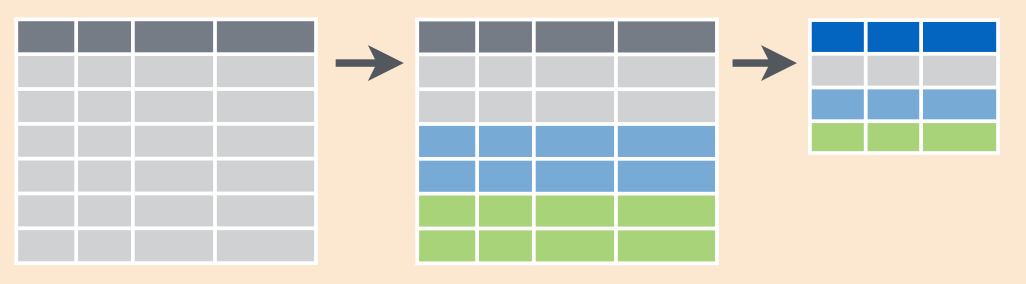
\includegraphics[width=4.16667in,height=\textheight]{images/group_by_s.png}

\hypertarget{sec-tidy_count}{%
\subsection{\texorpdfstring{Подсчет строк: \texttt{dplyr::n()},
\texttt{dplyr::count()}}{Подсчет строк: dplyr::n(), dplyr::count()}}\label{sec-tidy_count}}

Для подсчет количества значений можно воспользоваться функцией
\texttt{n()}.

\begin{Shaded}
\begin{Highlighting}[]
\NormalTok{heroes }\SpecialCharTok{\%\textgreater{}\%}
  \FunctionTok{group\_by}\NormalTok{(Gender) }\SpecialCharTok{\%\textgreater{}\%}
  \FunctionTok{summarise}\NormalTok{(}\AttributeTok{n =} \FunctionTok{n}\NormalTok{())}
\end{Highlighting}
\end{Shaded}

\begin{verbatim}
# A tibble: 3 x 2
  Gender     n
  <chr>  <int>
1 Female   200
2 Male     505
3 <NA>      29
\end{verbatim}

Функция \texttt{n()} вместе с \texttt{group\_by()} внутри
\texttt{filter()} позволяет удобным образом ``отрезать'' от тиббла
редкие группы\ldots{}

\begin{Shaded}
\begin{Highlighting}[]
\NormalTok{heroes }\SpecialCharTok{\%\textgreater{}\%}
  \FunctionTok{group\_by}\NormalTok{(Race) }\SpecialCharTok{\%\textgreater{}\%}
  \FunctionTok{filter}\NormalTok{(}\FunctionTok{n}\NormalTok{() }\SpecialCharTok{\textgreater{}} \DecValTok{10}\NormalTok{) }\SpecialCharTok{\%\textgreater{}\%}
  \FunctionTok{select}\NormalTok{(name, Race)}
\end{Highlighting}
\end{Shaded}

\begin{verbatim}
# A tibble: 611 x 2
# Groups:   Race [6]
   name          Race             
   <chr>         <chr>            
 1 A-Bomb        Human            
 2 Abomination   Human / Radiation
 3 Absorbing Man Human            
 4 Adam Monroe   <NA>             
 5 Adam Strange  Human            
 6 Agent 13      <NA>             
 7 Agent Bob     Human            
 8 Agent Zero    <NA>             
 9 Air-Walker    <NA>             
10 Ajax          Cyborg           
# i 601 more rows
\end{verbatim}

или же наоборот, выделить только маленькие группы:

\begin{Shaded}
\begin{Highlighting}[]
\NormalTok{heroes }\SpecialCharTok{\%\textgreater{}\%}
  \FunctionTok{group\_by}\NormalTok{(Race) }\SpecialCharTok{\%\textgreater{}\%}
  \FunctionTok{filter}\NormalTok{(}\FunctionTok{n}\NormalTok{() }\SpecialCharTok{==} \DecValTok{1}\NormalTok{) }\SpecialCharTok{\%\textgreater{}\%}
  \FunctionTok{select}\NormalTok{(name, Race)}
\end{Highlighting}
\end{Shaded}

\begin{verbatim}
# A tibble: 34 x 2
# Groups:   Race [34]
   name          Race              
   <chr>         <chr>             
 1 Abe Sapien    Icthyo Sapien     
 2 Abin Sur      Ungaran           
 3 Alien         Xenomorph XX121   
 4 Azazel        Neyaphem          
 5 Bizarro       Bizarro           
 6 Boba Fett     Human / Clone     
 7 Darth Maul    Dathomirian Zabrak
 8 Fin Fang Foom Kakarantharaian   
 9 Gamora        Zen-Whoberian     
10 Gladiator     Strontian         
# i 24 more rows
\end{verbatim}

Таблицу частот можно создать без \texttt{group\_by()} и
\texttt{summarise(n\ =\ n())}. Функция \texttt{count()} заменяет эту
конструкцию:

\begin{Shaded}
\begin{Highlighting}[]
\NormalTok{heroes }\SpecialCharTok{\%\textgreater{}\%}
  \FunctionTok{count}\NormalTok{(Gender)}
\end{Highlighting}
\end{Shaded}

\begin{verbatim}
# A tibble: 3 x 2
  Gender     n
  <chr>  <int>
1 Female   200
2 Male     505
3 <NA>      29
\end{verbatim}

Эту таблицу частот удобно сразу проранжировать, указав в параметре
\texttt{sort\ =} значение \texttt{TRUE}.

\begin{Shaded}
\begin{Highlighting}[]
\NormalTok{heroes }\SpecialCharTok{\%\textgreater{}\%}
  \FunctionTok{count}\NormalTok{(Gender, }\AttributeTok{sort =} \ConstantTok{TRUE}\NormalTok{)}
\end{Highlighting}
\end{Shaded}

\begin{verbatim}
# A tibble: 3 x 2
  Gender     n
  <chr>  <int>
1 Male     505
2 Female   200
3 <NA>      29
\end{verbatim}

\begin{quote}
Функция \texttt{count()}, несмотря на свою простоту, является одной из
наиболее используемых в tidyverse.
\end{quote}

\hypertarget{sec-tidy_distinct}{%
\subsection{\texorpdfstring{Уникальные значения:
\texttt{dplyr::distinct()}}{Уникальные значения: dplyr::distinct()}}\label{sec-tidy_distinct}}

\texttt{dplyr::distinct()} - это более быстрый аналог \texttt{unique()},
позволяет извлекать уникальные значения для одной или нескольких
колонок.

\begin{Shaded}
\begin{Highlighting}[]
\NormalTok{heroes }\SpecialCharTok{\%\textgreater{}\%}
  \FunctionTok{distinct}\NormalTok{(Gender)}
\end{Highlighting}
\end{Shaded}

\begin{verbatim}
# A tibble: 3 x 1
  Gender
  <chr> 
1 Male  
2 Female
3 <NA>  
\end{verbatim}

\begin{Shaded}
\begin{Highlighting}[]
\NormalTok{heroes }\SpecialCharTok{\%\textgreater{}\%}
  \FunctionTok{distinct}\NormalTok{(Gender, Race)}
\end{Highlighting}
\end{Shaded}

\begin{verbatim}
# A tibble: 81 x 2
   Gender Race             
   <chr>  <chr>            
 1 Male   Human            
 2 Male   Icthyo Sapien    
 3 Male   Ungaran          
 4 Male   Human / Radiation
 5 Male   Cosmic Entity    
 6 Male   <NA>             
 7 Female <NA>             
 8 Male   Cyborg           
 9 Male   Xenomorph XX121  
10 Male   Android          
# i 71 more rows
\end{verbatim}

Иногда нужно аггрегировать данные, но при этом сохранить исходную
структуру тиббла. Например, нужно посчитать размер групп или посчитать
средние значения по группе для последующего сравнения с индивидуальными
значениями.

\hypertarget{sec-tidy_group_mutate}{%
\subsection{Создание колонок с
группировкой}\label{sec-tidy_group_mutate}}

В tidyverse это можно сделать с помощью сочетания \texttt{group\_by()} и
\texttt{mutate()} (вместо \texttt{summarise()}):

\begin{Shaded}
\begin{Highlighting}[]
\NormalTok{heroes }\SpecialCharTok{\%\textgreater{}\%}
  \FunctionTok{group\_by}\NormalTok{(Race) }\SpecialCharTok{\%\textgreater{}\%}
  \FunctionTok{mutate}\NormalTok{(}\AttributeTok{Race\_n =} \FunctionTok{n}\NormalTok{()) }\SpecialCharTok{\%\textgreater{}\%}
  \FunctionTok{select}\NormalTok{(Race, name, Gender, Race\_n)}
\end{Highlighting}
\end{Shaded}

\begin{verbatim}
# A tibble: 734 x 4
# Groups:   Race [62]
   Race              name          Gender Race_n
   <chr>             <chr>         <chr>   <int>
 1 Human             A-Bomb        Male      208
 2 Icthyo Sapien     Abe Sapien    Male        1
 3 Ungaran           Abin Sur      Male        1
 4 Human / Radiation Abomination   Male       11
 5 Cosmic Entity     Abraxas       Male        4
 6 Human             Absorbing Man Male      208
 7 <NA>              Adam Monroe   Male      304
 8 Human             Adam Strange  Male      208
 9 <NA>              Agent 13      Female    304
10 Human             Agent Bob     Male      208
# i 724 more rows
\end{verbatim}

Результаты аггрегации были записаны в отдельную колонку, при этом
значения этой колонки внутри одной группы повторяются:

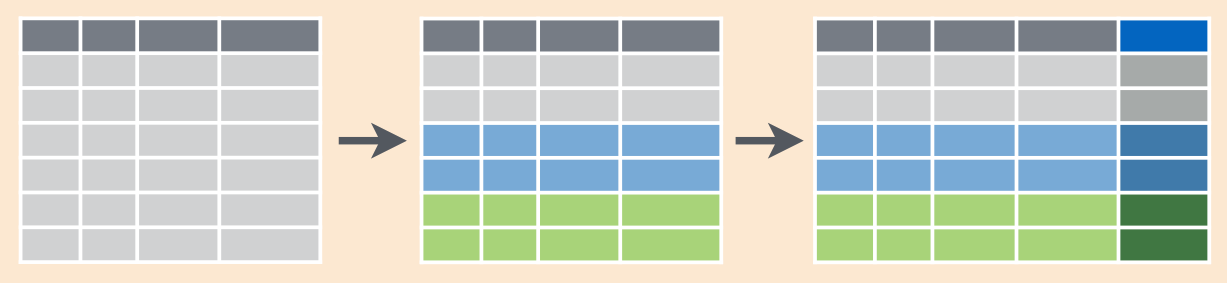
\includegraphics[width=4.16667in,height=\textheight]{images/group_by_m.png}

\hypertarget{sec-tidyverse_advanced}{%
\chapter{Продвинутый tidyverse}\label{sec-tidyverse_advanced}}

\hypertarget{sec-tidy_several}{%
\section{Объединение нескольких датафреймов}\label{sec-tidy_several}}

\hypertarget{sec-tidy_bind}{%
\subsection{Соединение структурно схожих датафреймов: bind\_rows(),
bind\_cols()}\label{sec-tidy_bind}}

Для начала подключим \texttt{tidyverse} и возьмем уже знакомый нам
датасет про супергероев:

\begin{Shaded}
\begin{Highlighting}[]
\FunctionTok{library}\NormalTok{(}\StringTok{"tidyverse"}\NormalTok{)}
\end{Highlighting}
\end{Shaded}

\begin{verbatim}
-- Attaching packages --------------------------------------- tidyverse 1.3.2 --
v ggplot2 3.4.2     v purrr   1.0.1
v tibble  3.2.1     v dplyr   1.1.2
v tidyr   1.3.0     v stringr 1.5.0
v readr   2.1.3     v forcats 1.0.0
-- Conflicts ------------------------------------------ tidyverse_conflicts() --
x dplyr::filter() masks stats::filter()
x dplyr::lag()    masks stats::lag()
\end{verbatim}

\begin{Shaded}
\begin{Highlighting}[]
\NormalTok{heroes }\OtherTok{\textless{}{-}} \FunctionTok{read\_csv}\NormalTok{(}\StringTok{"https://raw.githubusercontent.com/Pozdniakov/tidy\_stats/master/data/heroes\_information.csv"}\NormalTok{,}
                   \AttributeTok{na =} \FunctionTok{c}\NormalTok{(}\StringTok{"{-}"}\NormalTok{, }\StringTok{"{-}99"}\NormalTok{))}
\end{Highlighting}
\end{Shaded}

\begin{verbatim}
New names:
* `` -> `...1`
\end{verbatim}

\begin{verbatim}
Warning: One or more parsing issues, call `problems()` on your data frame for details,
e.g.:
  dat <- vroom(...)
  problems(dat)
\end{verbatim}

\begin{verbatim}
Rows: 734 Columns: 11
-- Column specification --------------------------------------------------------
Delimiter: ","
chr (8): name, Gender, Eye color, Race, Hair color, Publisher, Skin color, A...
dbl (3): ...1, Height, Weight

i Use `spec()` to retrieve the full column specification for this data.
i Specify the column types or set `show_col_types = FALSE` to quiet this message.
\end{verbatim}

Теперь создадим следующие тибблы и сохраним их как \texttt{dc},
\texttt{marvel} и \texttt{other\_publishers}:

\begin{Shaded}
\begin{Highlighting}[]
\NormalTok{dc }\OtherTok{\textless{}{-}}\NormalTok{ heroes }\SpecialCharTok{\%\textgreater{}\%}
  \FunctionTok{filter}\NormalTok{(Publisher }\SpecialCharTok{==} \StringTok{"DC Comics"}\NormalTok{) }\SpecialCharTok{\%\textgreater{}\%}
  \FunctionTok{group\_by}\NormalTok{(Gender) }\SpecialCharTok{\%\textgreater{}\%}
  \FunctionTok{summarise}\NormalTok{(}\AttributeTok{weight\_mean =} \FunctionTok{mean}\NormalTok{(Weight, }\AttributeTok{na.rm =} \ConstantTok{TRUE}\NormalTok{))}
\NormalTok{dc}
\end{Highlighting}
\end{Shaded}

\begin{verbatim}
# A tibble: 3 x 2
  Gender weight_mean
  <chr>        <dbl>
1 Female        76.8
2 Male         113. 
3 <NA>         NaN  
\end{verbatim}

\begin{Shaded}
\begin{Highlighting}[]
\NormalTok{marvel }\OtherTok{\textless{}{-}}\NormalTok{ heroes }\SpecialCharTok{\%\textgreater{}\%}
  \FunctionTok{filter}\NormalTok{(Publisher }\SpecialCharTok{==} \StringTok{"Marvel Comics"}\NormalTok{) }\SpecialCharTok{\%\textgreater{}\%}
  \FunctionTok{group\_by}\NormalTok{(Gender) }\SpecialCharTok{\%\textgreater{}\%}
  \FunctionTok{summarise}\NormalTok{(}\AttributeTok{weight\_mean =} \FunctionTok{mean}\NormalTok{(Weight, }\AttributeTok{na.rm =} \ConstantTok{TRUE}\NormalTok{))}
\NormalTok{marvel}
\end{Highlighting}
\end{Shaded}

\begin{verbatim}
# A tibble: 3 x 2
  Gender weight_mean
  <chr>        <dbl>
1 Female        80.1
2 Male         134. 
3 <NA>         129. 
\end{verbatim}

\begin{Shaded}
\begin{Highlighting}[]
\NormalTok{other\_publishers }\OtherTok{\textless{}{-}}\NormalTok{ heroes }\SpecialCharTok{\%\textgreater{}\%}
  \FunctionTok{filter}\NormalTok{(}\SpecialCharTok{!}\NormalTok{(Publisher }\SpecialCharTok{\%in\%} \FunctionTok{c}\NormalTok{(}\StringTok{"DC Comics"}\NormalTok{,}\StringTok{"Marvel Comics"}\NormalTok{))) }\SpecialCharTok{\%\textgreater{}\%}
  \FunctionTok{group\_by}\NormalTok{(Gender) }\SpecialCharTok{\%\textgreater{}\%}
  \FunctionTok{summarise}\NormalTok{(}\AttributeTok{weight\_mean =} \FunctionTok{mean}\NormalTok{(Weight, }\AttributeTok{na.rm =} \ConstantTok{TRUE}\NormalTok{))}
\NormalTok{other\_publishers}
\end{Highlighting}
\end{Shaded}

\begin{verbatim}
# A tibble: 3 x 2
  Gender weight_mean
  <chr>        <dbl>
1 Female        70.8
2 Male         111. 
3 <NA>         NaN  
\end{verbatim}

Несколько тибблов можно объединить вертикально с помощью функции
\texttt{bind\_rows()}. Для корректного объединения тибблы должны иметь
одинаковые названия колонок.

\begin{Shaded}
\begin{Highlighting}[]
\FunctionTok{bind\_rows}\NormalTok{(dc, marvel)}
\end{Highlighting}
\end{Shaded}

\begin{verbatim}
# A tibble: 6 x 2
  Gender weight_mean
  <chr>        <dbl>
1 Female        76.8
2 Male         113. 
3 <NA>         NaN  
4 Female        80.1
5 Male         134. 
6 <NA>         129. 
\end{verbatim}

Чтобы соединить тибблы горизонтально, воспользуйтесь функцией
\texttt{bind\_cols()}.

\begin{Shaded}
\begin{Highlighting}[]
\FunctionTok{bind\_cols}\NormalTok{(dc, marvel)}
\end{Highlighting}
\end{Shaded}

\begin{verbatim}
New names:
* `Gender` -> `Gender...1`
* `weight_mean` -> `weight_mean...2`
* `Gender` -> `Gender...3`
* `weight_mean` -> `weight_mean...4`
\end{verbatim}

\begin{verbatim}
# A tibble: 3 x 4
  Gender...1 weight_mean...2 Gender...3 weight_mean...4
  <chr>                <dbl> <chr>                <dbl>
1 Female                76.8 Female                80.1
2 Male                 113.  Male                 134. 
3 <NA>                 NaN   <NA>                 129. 
\end{verbatim}

Функции \texttt{bind\_rows()} и \texttt{bind\_cols()} могут работать не
только с двумя, но сразу с несколькими датафреймами.

\begin{Shaded}
\begin{Highlighting}[]
\FunctionTok{bind\_rows}\NormalTok{(dc, marvel, other\_publishers)}
\end{Highlighting}
\end{Shaded}

\begin{verbatim}
# A tibble: 9 x 2
  Gender weight_mean
  <chr>        <dbl>
1 Female        76.8
2 Male         113. 
3 <NA>         NaN  
4 Female        80.1
5 Male         134. 
6 <NA>         129. 
7 Female        70.8
8 Male         111. 
9 <NA>         NaN  
\end{verbatim}

На входе в функции \texttt{bind\_rows()} и \texttt{bind\_cold()} можно
подавать как сами датафреймы или тибблы через запятую, так и список из
датафреймов/тибблов.

\begin{Shaded}
\begin{Highlighting}[]
\NormalTok{heroes\_list\_of\_df }\OtherTok{\textless{}{-}} \FunctionTok{list}\NormalTok{(}\AttributeTok{DC =}\NormalTok{ dc, }
                          \AttributeTok{Marvel =}\NormalTok{ marvel, }
                          \AttributeTok{Other =}\NormalTok{ other\_publishers)}
\FunctionTok{bind\_rows}\NormalTok{(heroes\_list\_of\_df)}
\end{Highlighting}
\end{Shaded}

\begin{verbatim}
# A tibble: 9 x 2
  Gender weight_mean
  <chr>        <dbl>
1 Female        76.8
2 Male         113. 
3 <NA>         NaN  
4 Female        80.1
5 Male         134. 
6 <NA>         129. 
7 Female        70.8
8 Male         111. 
9 <NA>         NaN  
\end{verbatim}

Чтобы не потерять, из какого датафрейма какие данные, можно указать
любое строковое значение (название будущей колонки) для необязательного
аргумента \texttt{.id\ =}.

\begin{Shaded}
\begin{Highlighting}[]
\FunctionTok{bind\_rows}\NormalTok{(heroes\_list\_of\_df, }\AttributeTok{.id =} \StringTok{"Publisher"}\NormalTok{)}
\end{Highlighting}
\end{Shaded}

\begin{verbatim}
# A tibble: 9 x 3
  Publisher Gender weight_mean
  <chr>     <chr>        <dbl>
1 DC        Female        76.8
2 DC        Male         113. 
3 DC        <NA>         NaN  
4 Marvel    Female        80.1
5 Marvel    Male         134. 
6 Marvel    <NA>         129. 
7 Other     Female        70.8
8 Other     Male         111. 
9 Other     <NA>         NaN  
\end{verbatim}

\texttt{bind\_rows()} обычно используется, когда ваши данные находятся в
разных файлах с одинаковой структурой. Тогда вы можете прочитать все
таблицы в папке, сохранить их в качестве списка из датафреймов и
объединить в один датафрейм с помощью \texttt{bind\_rows()}.

\hypertarget{sec-tidy_join}{%
\subsection{\texorpdfstring{Реляционные данные:
\texttt{*\_join()}}{Реляционные данные: *\_join()}}\label{sec-tidy_join}}

В реальности иногда возникает ситуация, когда нужно соединить две
таблички, у которых есть общий столбец (или несколько столбцов), но все
остальные столбцы различаются. Табличек может быть и больше, это может
быть целая сеть таблиц, некоторые из которых содержат основные данные, а
некоторые - дополнительные, которые необходимо на определенном этапе
``включить'' в анализ. Например, таблица с расшифровкой аббревиатур или
сокращений вроде коротких названий стран или таблица телефонных кодов
разных стран. Совокупность нескольких связанных друг с другом таблиц
называют реляционными данными.

В случае с реляционными данными простых \texttt{bind\_rows()} и
\texttt{bind\_cols()} становится недостаточно.

Эти две таблички нужно объединить \textbf{(\emph{join}).} Эта задача
обычно возникает не очень часто, обычно это происходит один-два раза в
одном проекте, когда нужно дополнить имеющиеся данные дополнительной
информацией извне или объединить два набора данных, обрабатывавшихся в
разных программах. Однако каждый раз, когда такая задача возникает, это
доставляет много боли. \texttt{dplyr} предлагает интуитивно понятный
инструмент для объединения реляционных данных - семейство функций
\texttt{*\_join()}.

Возьмем для примера два тиббла \texttt{band\_members} и
\texttt{band\_instruments}, встроенных в \texttt{dplyr} специально для
демонстрации работы функций \texttt{*\_join()}.

\begin{Shaded}
\begin{Highlighting}[]
\NormalTok{band\_members}
\end{Highlighting}
\end{Shaded}

\begin{verbatim}
# A tibble: 3 x 2
  name  band   
  <chr> <chr>  
1 Mick  Stones 
2 John  Beatles
3 Paul  Beatles
\end{verbatim}

\begin{Shaded}
\begin{Highlighting}[]
\NormalTok{band\_instruments}
\end{Highlighting}
\end{Shaded}

\begin{verbatim}
# A tibble: 3 x 2
  name  plays 
  <chr> <chr> 
1 John  guitar
2 Paul  bass  
3 Keith guitar
\end{verbatim}

У этих двух тибблов есть колонка с одинаковым названием, которая по
своему смыслу соединяет данные обоих тибблов. Такая колонка называется
\textbf{ключом}. Ключ должен однозначно идентифицировать
наблюдения\footnote{Если ключи будут неуникальными, то функции
  \texttt{*\_join()} не будут выдавать ошибку. Вместо этого они добавят
  в итоговую таблицу все возможные пересечения повторяющихся ключей. С
  этим нужно быть очень осторожным, поэтому рекомендуется, во-первых,
  проверять уникальность ключей на входе и, во-вторых, проверять тиббл
  на выходе. Ну или использовать эту особенность работы функции
  \texttt{*\_join()} себе во благо.}.

Давайте попробуем посоединять \texttt{band\_members} и
\texttt{band\_instruments} разными вариантами \texttt{*\_join()} и
посмотрим, что у нас получится. Все эти функции имеют на входе два
обязательных аргумента (\texttt{x\ =} и \texttt{y\ =}) в которые мы
должны подставить два датафрейма/тиббла которые мы хотим объединить.
Главное различие между этими функциями заключается в том, что они будут
делать, если уникальные значения в ключах \texttt{x} и \texttt{y} не
соответствуют друг другу.

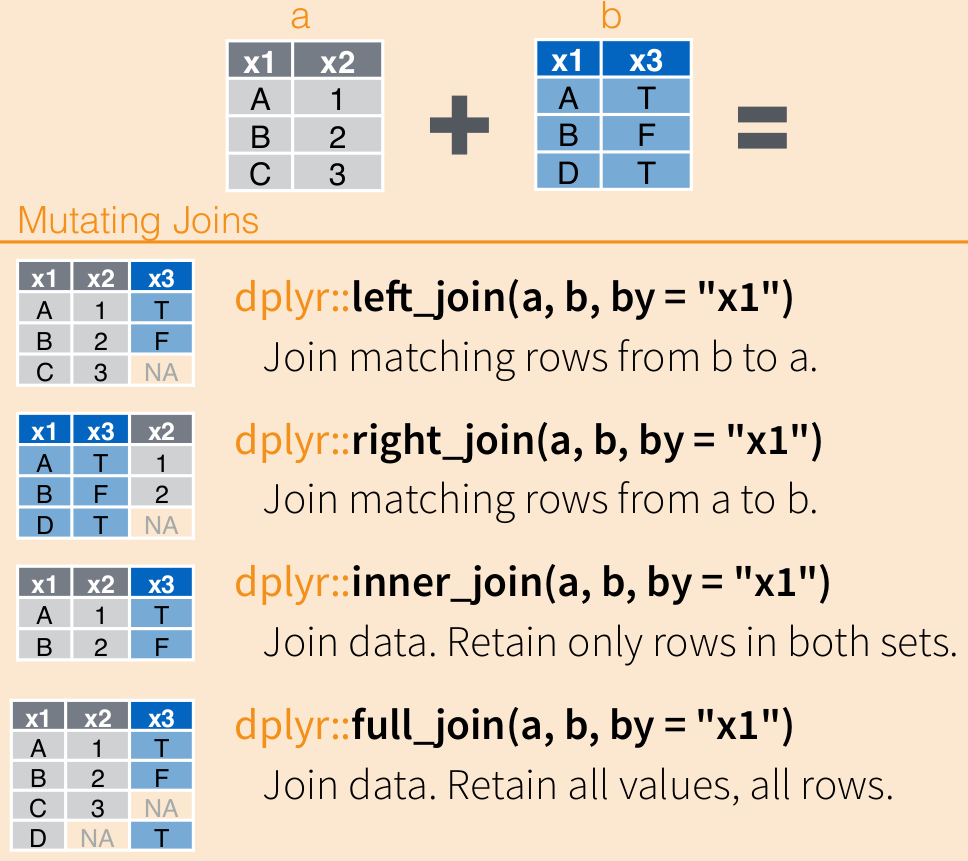
\includegraphics[width=4.16667in,height=\textheight]{images/joins.png}

\begin{itemize}
\tightlist
\item
  \texttt{left\_join()}:
\end{itemize}

\begin{Shaded}
\begin{Highlighting}[]
\NormalTok{band\_members }\SpecialCharTok{\%\textgreater{}\%}
  \FunctionTok{left\_join}\NormalTok{(band\_instruments)}
\end{Highlighting}
\end{Shaded}

\begin{verbatim}
Joining with `by = join_by(name)`
\end{verbatim}

\begin{verbatim}
# A tibble: 3 x 3
  name  band    plays 
  <chr> <chr>   <chr> 
1 Mick  Stones  <NA>  
2 John  Beatles guitar
3 Paul  Beatles bass  
\end{verbatim}

\texttt{left\_join()} - это самая простая для понимания и самая
используемая функция из семейства \texttt{*\_join()}. Она как бы
``дополняет'' информацию из первого тиббла вторым тибблом. В этом случае
сохраняются все уникальные наблюдения в \texttt{x}, но отбрасываются
лишние наблюдения в тиббле \texttt{y}. Тем значениям, которым не нашлось
соотвествия в \texttt{y}, в колонках, взятых их \texttt{y}, ставятся
значения \texttt{NA}.

Вы можете сами задать колонки-ключи параметром \texttt{by\ =}, по
умолчанию это все колонки с одинаковыми названиями в двух тибблах.

\begin{Shaded}
\begin{Highlighting}[]
\NormalTok{band\_members }\SpecialCharTok{\%\textgreater{}\%}
  \FunctionTok{left\_join}\NormalTok{(band\_instruments, }\AttributeTok{by =} \StringTok{"name"}\NormalTok{)}
\end{Highlighting}
\end{Shaded}

\begin{verbatim}
# A tibble: 3 x 3
  name  band    plays 
  <chr> <chr>   <chr> 
1 Mick  Stones  <NA>  
2 John  Beatles guitar
3 Paul  Beatles bass  
\end{verbatim}

Часто случается, что колонки-ключи называются по-разному в двух тибблах.
Их необязательно переименовывать, можно поставить соответстие вручную
используя проименованный вектор:

\begin{Shaded}
\begin{Highlighting}[]
\NormalTok{band\_members }\SpecialCharTok{\%\textgreater{}\%}
  \FunctionTok{left\_join}\NormalTok{(band\_instruments2, }\AttributeTok{by =} \FunctionTok{c}\NormalTok{(}\StringTok{"name"} \OtherTok{=} \StringTok{"artist"}\NormalTok{))}
\end{Highlighting}
\end{Shaded}

\begin{verbatim}
# A tibble: 3 x 3
  name  band    plays 
  <chr> <chr>   <chr> 
1 Mick  Stones  <NA>  
2 John  Beatles guitar
3 Paul  Beatles bass  
\end{verbatim}

\begin{itemize}
\tightlist
\item
  \texttt{right\_join()}:
\end{itemize}

\begin{Shaded}
\begin{Highlighting}[]
\NormalTok{band\_members }\SpecialCharTok{\%\textgreater{}\%}
  \FunctionTok{right\_join}\NormalTok{(band\_instruments)}
\end{Highlighting}
\end{Shaded}

\begin{verbatim}
Joining with `by = join_by(name)`
\end{verbatim}

\begin{verbatim}
# A tibble: 3 x 3
  name  band    plays 
  <chr> <chr>   <chr> 
1 John  Beatles guitar
2 Paul  Beatles bass  
3 Keith <NA>    guitar
\end{verbatim}

\texttt{right\_join()} отбрасывает строчки в \texttt{x}, которых не было
в \texttt{y}, но сохраняет соответствующие строчки \texttt{y} -
\texttt{left\_join()} наоборот.

\begin{itemize}
\tightlist
\item
  \texttt{full\_join()}:
\end{itemize}

\begin{Shaded}
\begin{Highlighting}[]
\NormalTok{band\_members }\SpecialCharTok{\%\textgreater{}\%}
  \FunctionTok{full\_join}\NormalTok{(band\_instruments)}
\end{Highlighting}
\end{Shaded}

\begin{verbatim}
Joining with `by = join_by(name)`
\end{verbatim}

\begin{verbatim}
# A tibble: 4 x 3
  name  band    plays 
  <chr> <chr>   <chr> 
1 Mick  Stones  <NA>  
2 John  Beatles guitar
3 Paul  Beatles bass  
4 Keith <NA>    guitar
\end{verbatim}

Функция \texttt{full\_join()} сохраняет все строчки и из \texttt{x} и
\texttt{y}. Пожалуй, наиболее используемая функция после
\texttt{left\_join()} -- благодаря \texttt{full\_join()} вы точно ничего
не потеряете при объединении.

\begin{itemize}
\tightlist
\item
  \texttt{inner\_join()}:
\end{itemize}

\begin{Shaded}
\begin{Highlighting}[]
\NormalTok{band\_members }\SpecialCharTok{\%\textgreater{}\%}
  \FunctionTok{inner\_join}\NormalTok{(band\_instruments)}
\end{Highlighting}
\end{Shaded}

\begin{verbatim}
Joining with `by = join_by(name)`
\end{verbatim}

\begin{verbatim}
# A tibble: 2 x 3
  name  band    plays 
  <chr> <chr>   <chr> 
1 John  Beatles guitar
2 Paul  Beatles bass  
\end{verbatim}

Функция \texttt{inner\_join()} сохраняет только строчки, которые
присутствуют и в \texttt{x}, и в \texttt{y}.

\begin{itemize}
\tightlist
\item
  \texttt{semi\_join()}:
\end{itemize}

\begin{Shaded}
\begin{Highlighting}[]
\NormalTok{band\_members }\SpecialCharTok{\%\textgreater{}\%}
  \FunctionTok{semi\_join}\NormalTok{(band\_instruments)}
\end{Highlighting}
\end{Shaded}

\begin{verbatim}
Joining with `by = join_by(name)`
\end{verbatim}

\begin{verbatim}
# A tibble: 2 x 2
  name  band   
  <chr> <chr>  
1 John  Beatles
2 Paul  Beatles
\end{verbatim}

\begin{itemize}
\tightlist
\item
  \texttt{anti\_join()}:
\end{itemize}

\begin{Shaded}
\begin{Highlighting}[]
\NormalTok{band\_members }\SpecialCharTok{\%\textgreater{}\%}
  \FunctionTok{anti\_join}\NormalTok{(band\_instruments)}
\end{Highlighting}
\end{Shaded}

\begin{verbatim}
Joining with `by = join_by(name)`
\end{verbatim}

\begin{verbatim}
# A tibble: 1 x 2
  name  band  
  <chr> <chr> 
1 Mick  Stones
\end{verbatim}

Функции \texttt{semi\_join()} и \texttt{anti\_join()} не присоединяют
второй датафрейм/тиббл (\texttt{y}) к первому. Вместо этого они
используются как некоторый словарь-фильтр для отделения только тех
значений в \texttt{x}, которые есть в \texttt{y} (\texttt{semi\_join()})
или, наоборот, которых нет в \texttt{y} (\texttt{anti\_join()}).

\hypertarget{sec-tidy_data}{%
\section{Tidy data: широкий и длинный форматы
данных}\label{sec-tidy_data}}

Принцип \textbf{\emph{tidy data}} предполагает, что каждая строка
содержит в себе одно измерение, каждая колонка - одну характеристику, а
в одной ячейке только одно значение. Тем не менее, это не говорит
однозначно о том, как именно хранить повторные измерения. Их можно
хранить в \textbf{широком формате \emph{(wide data)}} как одну колонку
для каждого измерения. Одной строчке соответствует один объект
измерения. Если измерений много, то такой датафрейм может получиться
очень широким.

Другой способ хранения данных в датафрейме -- \textbf{длинный формат
\emph{(long data).}} В этом случае создаются две колонки: одна колонка -
для идентификатора измерения (например, время измерения), другая колонка
- для записи самого измерения. Каждая строка соответствует одному
измерению объекта, а объект измерения имеет несколько строк в
датафрейме. Если измерений много, то датафрейм становится очень длинным.

Это лучше пояснить на примере. Например, измерим массу студентов до и
после прохождения курса по R. Как это лучше записать - \textbf{в широком
формате,} как два числовых столбца (один -- измерение до, второй --
измерение после)? Или же \textbf{в длинном формате:} создать строковую
колонку, в которой будет написано время измерения (``До курса по R'',
``После курса по R'') и числовую колонку со значением массы?

\begin{itemize}
\tightlist
\item
  \textbf{Широкий формат:}
\end{itemize}

\begin{longtable}[]{@{}lll@{}}
\toprule()
Студент & До курса по R & После курса по R \\
\midrule()
\endhead
Маша & 70 & 63 \\
Рома & 80 & 74 \\
Антонина & 86 & 71 \\
\bottomrule()
\end{longtable}

\begin{itemize}
\tightlist
\item
  \textbf{Длинный формат:}
\end{itemize}

\begin{longtable}[]{@{}lll@{}}
\toprule()
Студент & Время измерения & Масса (кг) \\
\midrule()
\endhead
Маша & До курса по R & 70 \\
Рома & До курса по R & 80 \\
Антонина & До курса по R & 86 \\
Маша & После курса по R & 63 \\
Рома & После курса по R & 74 \\
Антонина & После курса по R & 71 \\
\bottomrule()
\end{longtable}

На самом деле, оба варианта приемлемы, оба варианта встречаются в
реальных данных, а разные функции и статистические пакеты могут
требовать от вас как \textbf{длинный,} так и \textbf{широкий форматы.}

Таким образом, нам нужно научиться переводить из широкого формата в
длинный и наоборот. Для этого в tidyverse есть функции:

\begin{itemize}
\item
  \texttt{tidyr::pivot\_longer()}: переводит из \textbf{широкого} в
  \textbf{длинный формат,}
\item
  \texttt{tidyr::pivot\_wider()}: переводит из \textbf{длинного} в
  \textbf{широкий формат.}
\end{itemize}

К сожалению, в PDF нельзя вставить .gif анимацию, посмотреть ее можно по
\href{https://github.com/Pozdniakov/tidy_stats/blob/master/images/tidyr-longer-wider.gif}{ссылке}

\begin{Shaded}
\begin{Highlighting}[]
\NormalTok{new\_diet }\OtherTok{\textless{}{-}} \FunctionTok{tibble}\NormalTok{(}
  \AttributeTok{student =} \FunctionTok{c}\NormalTok{(}\StringTok{"Маша"}\NormalTok{, }\StringTok{"Рома"}\NormalTok{, }\StringTok{"Антонина"}\NormalTok{),}
  \AttributeTok{before\_r\_course =} \FunctionTok{c}\NormalTok{(}\DecValTok{70}\NormalTok{, }\DecValTok{80}\NormalTok{, }\DecValTok{86}\NormalTok{),}
  \AttributeTok{after\_r\_course =} \FunctionTok{c}\NormalTok{(}\DecValTok{63}\NormalTok{, }\DecValTok{74}\NormalTok{, }\DecValTok{71}\NormalTok{)}
\NormalTok{)}
\NormalTok{new\_diet}
\end{Highlighting}
\end{Shaded}

\begin{verbatim}
# A tibble: 3 x 3
  student  before_r_course after_r_course
  <chr>              <dbl>          <dbl>
1 Маша                  70             63
2 Рома                  80             74
3 Антонина              86             71
\end{verbatim}

Тиббл \texttt{new\_diet} - это пример широкого формата данных.

Превратим тиббл \texttt{new\_diet} длинный:

\begin{Shaded}
\begin{Highlighting}[]
\NormalTok{new\_diet }\SpecialCharTok{\%\textgreater{}\%}
  \FunctionTok{pivot\_longer}\NormalTok{(}\AttributeTok{cols =}\NormalTok{ before\_r\_course}\SpecialCharTok{:}\NormalTok{after\_r\_course,}
               \AttributeTok{names\_to =} \StringTok{"measurement\_time"}\NormalTok{, }
               \AttributeTok{values\_to =} \StringTok{"weight\_kg"}\NormalTok{)}
\end{Highlighting}
\end{Shaded}

\begin{verbatim}
# A tibble: 6 x 3
  student  measurement_time weight_kg
  <chr>    <chr>                <dbl>
1 Маша     before_r_course         70
2 Маша     after_r_course          63
3 Рома     before_r_course         80
4 Рома     after_r_course          74
5 Антонина before_r_course         86
6 Антонина after_r_course          71
\end{verbatim}

А теперь обратно в короткий:

\begin{Shaded}
\begin{Highlighting}[]
\NormalTok{new\_diet }\SpecialCharTok{\%\textgreater{}\%}
  \FunctionTok{pivot\_longer}\NormalTok{(}\AttributeTok{cols =}\NormalTok{ before\_r\_course}\SpecialCharTok{:}\NormalTok{after\_r\_course,}
               \AttributeTok{names\_to =} \StringTok{"measurement\_time"}\NormalTok{, }
               \AttributeTok{values\_to =} \StringTok{"weight\_kg"}\NormalTok{) }\SpecialCharTok{\%\textgreater{}\%}
  \FunctionTok{pivot\_wider}\NormalTok{(}\AttributeTok{names\_from =} \StringTok{"measurement\_time"}\NormalTok{,}
              \AttributeTok{values\_from =} \StringTok{"weight\_kg"}\NormalTok{)}
\end{Highlighting}
\end{Shaded}

\begin{verbatim}
# A tibble: 3 x 3
  student  before_r_course after_r_course
  <chr>              <dbl>          <dbl>
1 Маша                  70             63
2 Рома                  80             74
3 Антонина              86             71
\end{verbatim}

\hypertarget{sec-tidy_across}{%
\section{\texorpdfstring{Трансформация нескольких колонок:
\texttt{dplyr::across()}}{Трансформация нескольких колонок: dplyr::across()}}\label{sec-tidy_across}}

Допустим, вы хотите посчитать среднюю массу и рост, группируя по полу
супергероев. Можно посчитать это внутри одного \texttt{summarise()},
использую запятую:

\begin{Shaded}
\begin{Highlighting}[]
\NormalTok{heroes }\SpecialCharTok{\%\textgreater{}\%}
  \FunctionTok{group\_by}\NormalTok{(Gender) }\SpecialCharTok{\%\textgreater{}\%}
  \FunctionTok{summarise}\NormalTok{(}\AttributeTok{height =} \FunctionTok{mean}\NormalTok{(Height, }\AttributeTok{na.rm =} \ConstantTok{TRUE}\NormalTok{),}
            \AttributeTok{weight =} \FunctionTok{mean}\NormalTok{(Weight, }\AttributeTok{na.rm =} \ConstantTok{TRUE}\NormalTok{))}
\end{Highlighting}
\end{Shaded}

\begin{verbatim}
# A tibble: 3 x 3
  Gender height weight
  <chr>   <dbl>  <dbl>
1 Female   175.   78.8
2 Male     192.  126. 
3 <NA>     177.  129. 
\end{verbatim}

Если таких колонок будет много, то это уже станет сильно неудобным, нам
придется много копировать код, а это чревато ошибками и очень скучно.

Поэтому в \texttt{dplyr} есть функция для операций над несколькими
колонками сразу: \texttt{dplyr::across()}\footnote{Функция
  \texttt{across()} появилась в пакете \texttt{dplyr} относительно
  недавно, до этого для работы с множественными колонками в tidyverse
  использовались многочисленные функции \texttt{*\_at()},
  \texttt{*\_if()}, \texttt{*\_all()}, например,
  \texttt{summarise\_at()}, \texttt{summarise\_if()},
  \texttt{summarize\_all()}. Эти функции до сих пор присутствуют в
  \texttt{dplyr}, но считаются устаревшими. Другая альтернатива -
  использование пакета \texttt{purrr} (Глава~\ref{sec-purrr}) или
  семейства функций \texttt{apply()} (Глава~\ref{sec-apply_f}).}. Эта
функция работает похожим образом на функции семейства \texttt{apply()} и
использует tidyselect для выбора колонок.

Таким образом, конструкции с функцией \texttt{across()} можно разбить на
три части:

\begin{enumerate}
\def\labelenumi{\arabic{enumi}.}
\tightlist
\item
  Выбор колонок с помощью tidyselect. Здесь работают все те приемы,
  которые мы изучили при выборе колонок (Глава~\ref{sec-tidyselect}).
\item
  Собственно применение функции \texttt{across()}. Первый аргумент
  \texttt{.col} -- колонки, выбранные на первом этапе с помощью
  tidyselect, по умолчанию это \texttt{everything()}, т.е. все колонки.
  Второй аргумент \texttt{.fns} -- это функция или целый список из
  функций, которые будут применены к выбранным колонкам. Если функции
  требуют дополнительных аргументов, то они могут быть перечислены
  внутри \texttt{across()}.
\item
  Использование \texttt{summarise()} или другой функции \texttt{dplyr}.
  В этом случае в качестве аргумента для функции используется результат
  работы функции \texttt{across()}.
\end{enumerate}

Вот такой вот бутерброд выходит. Давайте посмотрим, как это работает на
практике и посчитаем среднее значение по колонкам \texttt{Height} и
\texttt{Weight}.

\begin{Shaded}
\begin{Highlighting}[]
\NormalTok{heroes }\SpecialCharTok{\%\textgreater{}\%}
  \FunctionTok{group\_by}\NormalTok{(Gender) }\SpecialCharTok{\%\textgreater{}\%}
  \FunctionTok{summarise}\NormalTok{(}\FunctionTok{across}\NormalTok{(}\FunctionTok{c}\NormalTok{(Height,Weight), mean))}
\end{Highlighting}
\end{Shaded}

\begin{verbatim}
# A tibble: 3 x 3
  Gender Height Weight
  <chr>   <dbl>  <dbl>
1 Female     NA     NA
2 Male       NA     NA
3 <NA>       NA     NA
\end{verbatim}

Здесь мы столкнулись с уже известной нам проблемой: функция
\texttt{mean()} при столкновении хотя бы с одним \texttt{NA} будет
возвращать \texttt{NA}, если мы не изменим параметр \texttt{na.rm\ =}.
Как и в случае с функциями семейства \texttt{apply()}
(Глава~\ref{sec-apply_f}), дополнительные параметры для функции можно
перечислить через запятую после самой функции:

\begin{Shaded}
\begin{Highlighting}[]
\NormalTok{heroes }\SpecialCharTok{\%\textgreater{}\%}
  \FunctionTok{group\_by}\NormalTok{(Gender) }\SpecialCharTok{\%\textgreater{}\%}
  \FunctionTok{summarise}\NormalTok{(}\FunctionTok{across}\NormalTok{(}\FunctionTok{c}\NormalTok{(Height, Weight), mean, }\AttributeTok{na.rm =} \ConstantTok{TRUE}\NormalTok{))}
\end{Highlighting}
\end{Shaded}

\begin{verbatim}
Warning: There was 1 warning in `summarise()`.
i In argument: `across(c(Height, Weight), mean, na.rm = TRUE)`.
i In group 1: `Gender = "Female"`.
Caused by warning:
! The `...` argument of `across()` is deprecated as of dplyr 1.1.0.
Supply arguments directly to `.fns` through an anonymous function instead.

  # Previously
  across(a:b, mean, na.rm = TRUE)

  # Now
  across(a:b, \(x) mean(x, na.rm = TRUE))
\end{verbatim}

\begin{verbatim}
# A tibble: 3 x 3
  Gender Height Weight
  <chr>   <dbl>  <dbl>
1 Female   175.   78.8
2 Male     192.  126. 
3 <NA>     177.  129. 
\end{verbatim}

До этого мы просто использовали выбор колонок по их названию. Но именно
внутри \texttt{across()} использование tidyselect раскрывается как
удивительно элегантный и мощный инструмент. Например, можно посчитать
среднее для всех numeric колонок:

\begin{Shaded}
\begin{Highlighting}[]
\NormalTok{heroes }\SpecialCharTok{\%\textgreater{}\%}
  \FunctionTok{drop\_na}\NormalTok{(Height, Weight) }\SpecialCharTok{\%\textgreater{}\%}
  \FunctionTok{group\_by}\NormalTok{(Gender) }\SpecialCharTok{\%\textgreater{}\%}
  \FunctionTok{summarise}\NormalTok{(}\FunctionTok{across}\NormalTok{(}\FunctionTok{where}\NormalTok{(is.numeric), mean, }\AttributeTok{na.rm =} \ConstantTok{TRUE}\NormalTok{))}
\end{Highlighting}
\end{Shaded}

\begin{verbatim}
# A tibble: 3 x 4
  Gender  ...1 Height Weight
  <chr>  <dbl>  <dbl>  <dbl>
1 Female  394.   174.   78.3
2 Male    369.   193.  126. 
3 <NA>    375.   182   129. 
\end{verbatim}

Или длину строк для строковых колонок. Для этого нам понадобится
вспомнить, как создавать анонимные функции (@ref(anon\_f)).

\begin{Shaded}
\begin{Highlighting}[]
\NormalTok{heroes }\SpecialCharTok{\%\textgreater{}\%}
  \FunctionTok{group\_by}\NormalTok{(Gender) }\SpecialCharTok{\%\textgreater{}\%}
  \FunctionTok{summarise}\NormalTok{(}\FunctionTok{across}\NormalTok{(}\FunctionTok{where}\NormalTok{(is.character), }
                   \ControlFlowTok{function}\NormalTok{(x) }\FunctionTok{mean}\NormalTok{(}\FunctionTok{nchar}\NormalTok{(x), }\AttributeTok{na.rm =} \ConstantTok{TRUE}\NormalTok{)))}
\end{Highlighting}
\end{Shaded}

\begin{verbatim}
# A tibble: 3 x 8
  Gender  name `Eye color`  Race `Hair color` Publisher `Skin color` Alignment
  <chr>  <dbl>       <dbl> <dbl>        <dbl>     <dbl>        <dbl>     <dbl>
1 Female  9.04        4.68  6.42         5.05      11.5         4.57      3.88
2 Male    9.05        4.53  6.75         5.48      11.4         5.02      3.78
3 <NA>    9.48        5.16 10.1          6.44      11.9         4         3.96
\end{verbatim}

Или же даже посчитать и то, и другое внутри одного \texttt{summarise()}!

\begin{Shaded}
\begin{Highlighting}[]
\NormalTok{heroes }\SpecialCharTok{\%\textgreater{}\%}
  \FunctionTok{group\_by}\NormalTok{(Gender) }\SpecialCharTok{\%\textgreater{}\%}
  \FunctionTok{summarise}\NormalTok{(}\FunctionTok{across}\NormalTok{(}\FunctionTok{where}\NormalTok{(is.numeric), mean, }\AttributeTok{na.rm =} \ConstantTok{TRUE}\NormalTok{),}
            \FunctionTok{across}\NormalTok{(}\FunctionTok{where}\NormalTok{(is.character), }
                   \ControlFlowTok{function}\NormalTok{(x) }\FunctionTok{mean}\NormalTok{(}\FunctionTok{nchar}\NormalTok{(x), }\AttributeTok{na.rm =} \ConstantTok{TRUE}\NormalTok{)))}
\end{Highlighting}
\end{Shaded}

\begin{verbatim}
# A tibble: 3 x 11
  Gender  ...1 Height Weight  name `Eye color`  Race `Hair color` Publisher
  <chr>  <dbl>  <dbl>  <dbl> <dbl>       <dbl> <dbl>        <dbl>     <dbl>
1 Female  395.   175.   78.8  9.04        4.68  6.42         5.05      11.5
2 Male    357.   192.  126.   9.05        4.53  6.75         5.48      11.4
3 <NA>    329    177.  129.   9.48        5.16 10.1          6.44      11.9
# i 2 more variables: `Skin color` <dbl>, Alignment <dbl>
\end{verbatim}

Внутри одного \texttt{across()} можно применить не одну функцию к каждой
из выбранных колонок, а сразу несколько функций для каждой из колонок.
Для этого нам нужно использовать список функций (желательно -
проименованный).

\begin{Shaded}
\begin{Highlighting}[]
\NormalTok{heroes }\SpecialCharTok{\%\textgreater{}\%}
  \FunctionTok{group\_by}\NormalTok{(Gender) }\SpecialCharTok{\%\textgreater{}\%}
  \FunctionTok{summarise}\NormalTok{(}\FunctionTok{across}\NormalTok{(}\FunctionTok{c}\NormalTok{(Height, Weight), }
                   \FunctionTok{list}\NormalTok{(}\AttributeTok{minimum =}\NormalTok{ min,}
                        \AttributeTok{average =}\NormalTok{ mean,}
                        \AttributeTok{maximum =}\NormalTok{ max), }
                   \AttributeTok{na.rm =} \ConstantTok{TRUE}\NormalTok{))}
\end{Highlighting}
\end{Shaded}

\begin{verbatim}
# A tibble: 3 x 7
  Gender Height_minimum Height_average Height_maximum Weight_minimum
  <chr>           <dbl>          <dbl>          <dbl>          <dbl>
1 Female           62.5           175.            366             41
2 Male             15.2           192.            975              2
3 <NA>            108             177.            198             39
# i 2 more variables: Weight_average <dbl>, Weight_maximum <dbl>
\end{verbatim}

\begin{quote}
Вот нам и понадобился список функций (@ref(functions\_objects))!
\end{quote}

\begin{Shaded}
\begin{Highlighting}[]
\NormalTok{heroes }\SpecialCharTok{\%\textgreater{}\%}
  \FunctionTok{group\_by}\NormalTok{(Gender) }\SpecialCharTok{\%\textgreater{}\%}
  \FunctionTok{summarise}\NormalTok{(}\FunctionTok{across}\NormalTok{(}\FunctionTok{c}\NormalTok{(Height, Weight),}
                   \FunctionTok{list}\NormalTok{(}\AttributeTok{min =} \ControlFlowTok{function}\NormalTok{(x) }\FunctionTok{min}\NormalTok{(x, }\AttributeTok{na.rm =} \ConstantTok{TRUE}\NormalTok{),}
                        \AttributeTok{mean =} \ControlFlowTok{function}\NormalTok{(x) }\FunctionTok{mean}\NormalTok{(x, }\AttributeTok{na.rm =} \ConstantTok{TRUE}\NormalTok{),}
                        \AttributeTok{max =} \ControlFlowTok{function}\NormalTok{(x) }\FunctionTok{max}\NormalTok{(x, }\AttributeTok{na.rm =} \ConstantTok{TRUE}\NormalTok{),}
                        \AttributeTok{na\_n =} \ControlFlowTok{function}\NormalTok{(x, ...) }\FunctionTok{sum}\NormalTok{(}\FunctionTok{is.na}\NormalTok{(x)))}
\NormalTok{                   )}
\NormalTok{            )}
\end{Highlighting}
\end{Shaded}

\begin{verbatim}
# A tibble: 3 x 9
  Gender Height_min Height_mean Height_max Height_na_n Weight_min Weight_mean
  <chr>       <dbl>       <dbl>      <dbl>       <int>      <dbl>       <dbl>
1 Female       62.5        175.        366          56         41        78.8
2 Male         15.2        192.        975         147          2       126. 
3 <NA>        108          177.        198          14         39       129. 
# i 2 more variables: Weight_max <dbl>, Weight_na_n <int>
\end{verbatim}

Хотя основное применение функции \texttt{across()} -- это массовое
подытоживание с помощью \texttt{summarise()}, \texttt{across()} можно
использовать и с другими функциями \texttt{dplyr}. Например, можно
делать массовые операции с колонками с помощью \texttt{mutate()}:

\begin{Shaded}
\begin{Highlighting}[]
\NormalTok{heroes }\SpecialCharTok{\%\textgreater{}\%}
  \FunctionTok{mutate}\NormalTok{(}\FunctionTok{across}\NormalTok{(}\FunctionTok{where}\NormalTok{(is.character), as.factor))}
\end{Highlighting}
\end{Shaded}

\begin{verbatim}
# A tibble: 734 x 11
    ...1 name          Gender `Eye color` Race     `Hair color` Height Publisher
   <dbl> <fct>         <fct>  <fct>       <fct>    <fct>         <dbl> <fct>    
 1     0 A-Bomb        Male   yellow      Human    No Hair         203 Marvel C~
 2     1 Abe Sapien    Male   blue        Icthyo ~ No Hair         191 Dark Hor~
 3     2 Abin Sur      Male   blue        Ungaran  No Hair         185 DC Comics
 4     3 Abomination   Male   green       Human /~ No Hair         203 Marvel C~
 5     4 Abraxas       Male   blue        Cosmic ~ Black            NA Marvel C~
 6     5 Absorbing Man Male   blue        Human    No Hair         193 Marvel C~
 7     6 Adam Monroe   Male   blue        <NA>     Blond            NA NBC - He~
 8     7 Adam Strange  Male   blue        Human    Blond           185 DC Comics
 9     8 Agent 13      Female blue        <NA>     Blond           173 Marvel C~
10     9 Agent Bob     Male   brown       Human    Brown           178 Marvel C~
# i 724 more rows
# i 3 more variables: `Skin color` <fct>, Alignment <fct>, Weight <dbl>
\end{verbatim}

Конструкция \texttt{across()} работает не только внутри
\texttt{summarise()} и \texttt{mutate()}, можно применять
\texttt{across()} и с другими функциями, которые используют
data-masking. Например, можно использовать \texttt{across()} внутри
\texttt{count()} вместе с функцией \texttt{n\_distinct()}, которая
считает количество уникальных значений в векторе. Это позволяет
посмотреть таблицу частот для группирующих переменных:

\begin{Shaded}
\begin{Highlighting}[]
\NormalTok{heroes }\SpecialCharTok{\%\textgreater{}\%}
  \FunctionTok{count}\NormalTok{(}\FunctionTok{across}\NormalTok{(}\FunctionTok{where}\NormalTok{(}\ControlFlowTok{function}\NormalTok{(x) }\FunctionTok{n\_distinct}\NormalTok{(x) }\SpecialCharTok{\textless{}=} \DecValTok{6}\NormalTok{)))}
\end{Highlighting}
\end{Shaded}

\begin{verbatim}
# A tibble: 11 x 3
   Gender Alignment     n
   <chr>  <chr>     <int>
 1 Female bad          35
 2 Female good        161
 3 Female neutral       4
 4 Male   bad         165
 5 Male   good        316
 6 Male   neutral      18
 7 Male   <NA>          6
 8 <NA>   bad           7
 9 <NA>   good         19
10 <NA>   neutral       2
11 <NA>   <NA>          1
\end{verbatim}

\hypertarget{sec-purrr}{%
\section{\texorpdfstring{Функциональное программирование:
\texttt{purrr}}{Функциональное программирование: purrr}}\label{sec-purrr}}

\texttt{purrr} -- это пакет для функционального программирования в
tidyverse. Как и многие пакеты tidyverse, \texttt{purrr} пытается
заменить собой базовый функционал R на более понятный и удобный. В
данном случае, речь в первую очередь идет о функциях семейства
\texttt{apply()}, с которыми мы работали ранее (@ref(apply\_f)).

Давайте вспомним, как работает \texttt{lapply()}. В качестве первого
аргумента функция \texttt{lapply()} принимает список (или то, что может
быть в него превращено, например, датафрейм), в качестве второго -
функцию, которая будет применена к каждому элементу списка. На выходе мы
получим список такой же длины.

\begin{Shaded}
\begin{Highlighting}[]
\FunctionTok{lapply}\NormalTok{(heroes, class)}
\end{Highlighting}
\end{Shaded}

\begin{verbatim}
$...1
[1] "numeric"

$name
[1] "character"

$Gender
[1] "character"

$`Eye color`
[1] "character"

$Race
[1] "character"

$`Hair color`
[1] "character"

$Height
[1] "numeric"

$Publisher
[1] "character"

$`Skin color`
[1] "character"

$Alignment
[1] "character"

$Weight
[1] "numeric"
\end{verbatim}

Функция \texttt{purrr::map()} работает по тому же принципу: можно просто
заменить \texttt{lapply()} на \texttt{map()}, и мы получим тот же
результат.

\begin{Shaded}
\begin{Highlighting}[]
\FunctionTok{map}\NormalTok{(heroes, class)}
\end{Highlighting}
\end{Shaded}

\begin{verbatim}
$...1
[1] "numeric"

$name
[1] "character"

$Gender
[1] "character"

$`Eye color`
[1] "character"

$Race
[1] "character"

$`Hair color`
[1] "character"

$Height
[1] "numeric"

$Publisher
[1] "character"

$`Skin color`
[1] "character"

$Alignment
[1] "character"

$Weight
[1] "numeric"
\end{verbatim}

\texttt{map()} можно встроить в канал с пайпом (впрочем, как и
\texttt{lapply()}):

\begin{Shaded}
\begin{Highlighting}[]
\NormalTok{heroes }\SpecialCharTok{\%\textgreater{}\%}
  \FunctionTok{map}\NormalTok{(class)}
\end{Highlighting}
\end{Shaded}

\begin{verbatim}
$...1
[1] "numeric"

$name
[1] "character"

$Gender
[1] "character"

$`Eye color`
[1] "character"

$Race
[1] "character"

$`Hair color`
[1] "character"

$Height
[1] "numeric"

$Publisher
[1] "character"

$`Skin color`
[1] "character"

$Alignment
[1] "character"

$Weight
[1] "numeric"
\end{verbatim}

Как и \texttt{lapply()}, \texttt{map()} всегда возвращает список. Из-за
этого мы больше пользовались функцией \texttt{sapply()}, а не
\texttt{lapply()}. Функция \texttt{sapply()} упрощала результат до
вектора, если это возможно. Подобное упрощение может показаться удобным
пока не сталкиваешься с тем, что иногда очень сложно предсказать, какой
тип данных получится на выходе. Есть функция \texttt{vapply()} в которой
можно управлять типом данных на выходе, но она не очень удобная. В
\texttt{purrr} эта проблема решена просто: есть множество функций
\texttt{map\_*()}, где вместо звездочки - нужный формат на выходе.

Например, если мы хотим получить строковый вектор на выходе, то нам
нужна функция \texttt{map\_chr()}.

\begin{Shaded}
\begin{Highlighting}[]
\NormalTok{heroes }\SpecialCharTok{\%\textgreater{}\%}
  \FunctionTok{map\_chr}\NormalTok{(class)}
\end{Highlighting}
\end{Shaded}

\begin{verbatim}
       ...1        name      Gender   Eye color        Race  Hair color 
  "numeric" "character" "character" "character" "character" "character" 
     Height   Publisher  Skin color   Alignment      Weight 
  "numeric" "character" "character" "character"   "numeric" 
\end{verbatim}

Можно превратить результат в датафрейм с помощью \texttt{map\_df()}.

\begin{Shaded}
\begin{Highlighting}[]
\NormalTok{heroes }\SpecialCharTok{\%\textgreater{}\%}
  \FunctionTok{map\_df}\NormalTok{(class)}
\end{Highlighting}
\end{Shaded}

\begin{verbatim}
# A tibble: 1 x 11
  ...1    name      Gender    `Eye color` Race     `Hair color` Height Publisher
  <chr>   <chr>     <chr>     <chr>       <chr>    <chr>        <chr>  <chr>    
1 numeric character character character   charact~ character    numer~ character
# i 3 more variables: `Skin color` <chr>, Alignment <chr>, Weight <chr>
\end{verbatim}

Так же как и функции семейства \texttt{apply()}, функции
\texttt{map\_*()} отлично сочетаются с анонимными функциями.

\begin{Shaded}
\begin{Highlighting}[]
\NormalTok{heroes }\SpecialCharTok{\%\textgreater{}\%}
  \FunctionTok{map\_int}\NormalTok{(}\ControlFlowTok{function}\NormalTok{(x) }\FunctionTok{sum}\NormalTok{(}\FunctionTok{is.na}\NormalTok{(x)))}
\end{Highlighting}
\end{Shaded}

\begin{verbatim}
      ...1       name     Gender  Eye color       Race Hair color     Height 
         0          0         29        172        304        172        217 
 Publisher Skin color  Alignment     Weight 
         0        662          7        239 
\end{verbatim}

Однако у \texttt{purrr} есть свой, более короткий способ записи
анонимных функций: \texttt{function(arg)} заменяется на
\texttt{\textasciitilde{}}, а \texttt{arg} на \texttt{.}.

\begin{Shaded}
\begin{Highlighting}[]
\NormalTok{heroes }\SpecialCharTok{\%\textgreater{}\%}
  \FunctionTok{map\_int}\NormalTok{(}\SpecialCharTok{\textasciitilde{}}\FunctionTok{sum}\NormalTok{(}\FunctionTok{is.na}\NormalTok{(.)))}
\end{Highlighting}
\end{Shaded}

\begin{verbatim}
      ...1       name     Gender  Eye color       Race Hair color     Height 
         0          0         29        172        304        172        217 
 Publisher Skin color  Alignment     Weight 
         0        662          7        239 
\end{verbatim}

Если нужно итерироваться сразу по нескольким спискам, то есть функции
\texttt{map2\_*()} (для двух списков) и \texttt{pmap\_*()} (для
нескольких списков).

\hypertarget{sec-list_colums_nest}{%
\section{\texorpdfstring{Колонки-списки и нестинг:
\texttt{nest()}}{Колонки-списки и нестинг: nest()}}\label{sec-list_colums_nest}}

Ранее мы говорили о том, что датафрейм -- это по своей сути список из
векторов разной длины. На самом деле, это не совсем так: колонки
обычного датафрейма вполне могут быть списками. Однако делать так обычно
не рекомендуется, пусть R это и не запрещает создавать такие колонки:
многие функции предполагают, что все колонки датафрейма являются
векторами.

\texttt{tidyverse} гораздо дружелюбнее относится к использовании списка
в качестве колонки. Такие колонки называются \textbf{колонками-списками
(list columns)}. Основной способ их создания - использования функции
\texttt{tidyr::nest()}. С помощью tidyselect нужно выбрать сжимаемые
колонки, которые будут агрегированы по невыбранным колонками. Это и
называется нестингом.

\begin{Shaded}
\begin{Highlighting}[]
\NormalTok{heroes }\SpecialCharTok{\%\textgreater{}\%}
  \FunctionTok{nest}\NormalTok{(}\SpecialCharTok{!}\NormalTok{Gender)}
\end{Highlighting}
\end{Shaded}

\begin{verbatim}
Warning: Supplying `...` without names was deprecated in tidyr 1.0.0.
i Please specify a name for each selection.
i Did you want `data = !Gender`?
\end{verbatim}

\begin{verbatim}
# A tibble: 3 x 2
  Gender data               
  <chr>  <list>             
1 Male   <tibble [505 x 10]>
2 Female <tibble [200 x 10]>
3 <NA>   <tibble [29 x 10]> 
\end{verbatim}

Заметьте, у нас появилась колонка \texttt{data}, в которой содержатся
тибблы. Туда и спрятались все наши данные.

Нестинг похож на агрегирование с помощью \texttt{group\_by()}. Если
сделать нестинг сгруппированного с помощью \texttt{group\_by()} тиббла,
то сожмутся все колонки кроме тех, которые выступают в качестве групп:

\begin{Shaded}
\begin{Highlighting}[]
\NormalTok{heroes }\SpecialCharTok{\%\textgreater{}\%}
  \FunctionTok{group\_by}\NormalTok{(Gender) }\SpecialCharTok{\%\textgreater{}\%}
  \FunctionTok{nest}\NormalTok{()}
\end{Highlighting}
\end{Shaded}

\begin{verbatim}
# A tibble: 3 x 2
# Groups:   Gender [3]
  Gender data               
  <chr>  <list>             
1 Male   <tibble [505 x 10]>
2 Female <tibble [200 x 10]>
3 <NA>   <tibble [29 x 10]> 
\end{verbatim}

Теперь можно работать с колонкой-списком как с обычной колонкой.
Например, применять функцию для каждой строчки (то есть для каждого
тиббла) с помощью \texttt{map()} и записывать результат в новую колонку
с помощью \texttt{mutate()}.

\begin{Shaded}
\begin{Highlighting}[]
\NormalTok{heroes }\SpecialCharTok{\%\textgreater{}\%}
  \FunctionTok{group\_by}\NormalTok{(Gender) }\SpecialCharTok{\%\textgreater{}\%}
  \FunctionTok{nest}\NormalTok{() }\SpecialCharTok{\%\textgreater{}\%}
  \FunctionTok{mutate}\NormalTok{(}\AttributeTok{dim =} \FunctionTok{map}\NormalTok{(data, dim))}
\end{Highlighting}
\end{Shaded}

\begin{verbatim}
# A tibble: 3 x 3
# Groups:   Gender [3]
  Gender data                dim      
  <chr>  <list>              <list>   
1 Male   <tibble [505 x 10]> <int [2]>
2 Female <tibble [200 x 10]> <int [2]>
3 <NA>   <tibble [29 x 10]>  <int [2]>
\end{verbatim}

В конце концов нам нужно ``разжать'' сжатую колонку-список. Сделать это
можно с помощью \texttt{unnest()}, выбрав с помощью tidyselect нужные
колонки.

\begin{Shaded}
\begin{Highlighting}[]
\NormalTok{heroes }\SpecialCharTok{\%\textgreater{}\%}
  \FunctionTok{group\_by}\NormalTok{(Gender) }\SpecialCharTok{\%\textgreater{}\%}
  \FunctionTok{nest}\NormalTok{() }\SpecialCharTok{\%\textgreater{}\%}
  \FunctionTok{mutate}\NormalTok{(}\AttributeTok{dim =} \FunctionTok{map}\NormalTok{(data, dim)) }\SpecialCharTok{\%\textgreater{}\%}
  \FunctionTok{unnest}\NormalTok{(dim)}
\end{Highlighting}
\end{Shaded}

\begin{verbatim}
# A tibble: 6 x 3
# Groups:   Gender [3]
  Gender data                  dim
  <chr>  <list>              <int>
1 Male   <tibble [505 x 10]>   505
2 Male   <tibble [505 x 10]>    10
3 Female <tibble [200 x 10]>   200
4 Female <tibble [200 x 10]>    10
5 <NA>   <tibble [29 x 10]>     29
6 <NA>   <tibble [29 x 10]>     10
\end{verbatim}

Разжатая колонка обычно больше сжатой, поэтому разжатие привело к
удлинению тиббла. Вместо удлинения тиббла, его можно расширить с помощью
\texttt{unnest\_wider()}.

\begin{Shaded}
\begin{Highlighting}[]
\NormalTok{heroes }\SpecialCharTok{\%\textgreater{}\%}
  \FunctionTok{group\_by}\NormalTok{(Gender) }\SpecialCharTok{\%\textgreater{}\%}
  \FunctionTok{nest}\NormalTok{() }\SpecialCharTok{\%\textgreater{}\%}
  \FunctionTok{mutate}\NormalTok{(}\AttributeTok{dim =} \FunctionTok{map}\NormalTok{(data, dim)) }\SpecialCharTok{\%\textgreater{}\%}
  \FunctionTok{unnest\_wider}\NormalTok{(dim, }\AttributeTok{names\_sep =} \StringTok{"\_"}\NormalTok{) }
\end{Highlighting}
\end{Shaded}

\begin{verbatim}
# A tibble: 3 x 4
# Groups:   Gender [3]
  Gender data                dim_1 dim_2
  <chr>  <list>              <int> <int>
1 Male   <tibble [505 x 10]>   505    10
2 Female <tibble [200 x 10]>   200    10
3 <NA>   <tibble [29 x 10]>     29    10
\end{verbatim}

Нестинг - это мощный инструмент tidyverse, хотя во многих случаях можно
обойтись и без него. Наиболее эффективна эта конструкция именно в тех
ситуациях, где вы делаете операции над целыми тибблами. Поэтому
наибольшее распространение нестинг получил в смычке с пакетом
\texttt{broom} для расчета множественных статистических моделей.

Другое применение нестинга -- решение проблемы с несколькими значениями
в одной ячейки, которые записаны через запятую или какой-либо другой
знак. Такое часто встречается в данных, поэтому хорошо бы уметь с этим
работать!

Возьмем небольшой искусственный пример:

\begin{Shaded}
\begin{Highlighting}[]
\NormalTok{films }\OtherTok{\textless{}{-}} \FunctionTok{tribble}\NormalTok{(}
  \SpecialCharTok{\textasciitilde{}}\NormalTok{film, }\SpecialCharTok{\textasciitilde{}}\NormalTok{genres,}
  \StringTok{"Ирония Судьбы"}\NormalTok{, }\StringTok{"comedy, drama"}\NormalTok{,}
  \StringTok{"Большой Лебовски"}\NormalTok{, }\StringTok{"comedy, criminal"}\NormalTok{,}
  \StringTok{"Аватар"}\NormalTok{, }\StringTok{"fantasy, drama"}
\NormalTok{)}

\NormalTok{films}
\end{Highlighting}
\end{Shaded}

\begin{verbatim}
# A tibble: 3 x 2
  film             genres          
  <chr>            <chr>           
1 Ирония Судьбы    comedy, drama   
2 Большой Лебовски comedy, criminal
3 Аватар           fantasy, drama  
\end{verbatim}

Для этого разобъем значения колонки \texttt{genres} с помощью встроенной
функции \texttt{strsplit()}. Она разбивает значения вектора по
выбранному разделителю. Здесь нам нужен разделитель \texttt{",\ "} (с
пробелом после запятой!). На выходе мы получим список такой же длины,
что и исходный вектором, а каждый элемент этого списка будет строковым
вектором. Количество значений внутри векторов может быть каким угодно.
Поскольку результат -- список, перезаписанная колонка \texttt{genres}
станет колонкой-списком.

\begin{Shaded}
\begin{Highlighting}[]
\NormalTok{films }\SpecialCharTok{\%\textgreater{}\%}
  \FunctionTok{mutate}\NormalTok{(}\AttributeTok{genres =} \FunctionTok{strsplit}\NormalTok{(genres, }\StringTok{", "}\NormalTok{))}
\end{Highlighting}
\end{Shaded}

\begin{verbatim}
# A tibble: 3 x 2
  film             genres   
  <chr>            <list>   
1 Ирония Судьбы    <chr [2]>
2 Большой Лебовски <chr [2]>
3 Аватар           <chr [2]>
\end{verbatim}

Теперь нам нужно сделать \texttt{unnest()}

\begin{Shaded}
\begin{Highlighting}[]
\NormalTok{films }\SpecialCharTok{\%\textgreater{}\%}
  \FunctionTok{mutate}\NormalTok{(}\AttributeTok{genres =} \FunctionTok{strsplit}\NormalTok{(genres, }\StringTok{", "}\NormalTok{)) }\SpecialCharTok{\%\textgreater{}\%}
  \FunctionTok{unnest}\NormalTok{()}
\end{Highlighting}
\end{Shaded}

\begin{verbatim}
Warning: `cols` is now required when using `unnest()`.
i Please use `cols = c(genres)`.
\end{verbatim}

\begin{verbatim}
# A tibble: 6 x 2
  film             genres  
  <chr>            <chr>   
1 Ирония Судьбы    comedy  
2 Ирония Судьбы    drama   
3 Большой Лебовски comedy  
4 Большой Лебовски criminal
5 Аватар           fantasy 
6 Аватар           drama   
\end{verbatim}

Теперь у нас данные в длинном виде! Результат можно расширить с помощью
уже знакомого \texttt{pivot\_wider()} и дополнительной колонки со
значениями \texttt{TRUE}. Если соответствующей пары нет в тиббле, то в
итоговой широкой таблице будет \texttt{NA}, мы можем поменять их на
\texttt{FALSE} с помощью параметра \texttt{values\_fill\ =}.

\begin{Shaded}
\begin{Highlighting}[]
\NormalTok{films }\SpecialCharTok{\%\textgreater{}\%}
  \FunctionTok{mutate}\NormalTok{(}\AttributeTok{genres =} \FunctionTok{strsplit}\NormalTok{(genres, }\StringTok{", "}\NormalTok{)) }\SpecialCharTok{\%\textgreater{}\%}
  \FunctionTok{unnest}\NormalTok{() }\SpecialCharTok{\%\textgreater{}\%}
  \FunctionTok{mutate}\NormalTok{(}\AttributeTok{value =} \ConstantTok{TRUE}\NormalTok{) }\SpecialCharTok{\%\textgreater{}\%}
  \FunctionTok{pivot\_wider}\NormalTok{(}\AttributeTok{names\_from =} \StringTok{"genres"}\NormalTok{,}
              \AttributeTok{values\_from =} \StringTok{"value"}\NormalTok{, }\AttributeTok{values\_fill =} \ConstantTok{FALSE}\NormalTok{)}
\end{Highlighting}
\end{Shaded}

\begin{verbatim}
Warning: `cols` is now required when using `unnest()`.
i Please use `cols = c(genres)`.
\end{verbatim}

\begin{verbatim}
# A tibble: 3 x 5
  film             comedy drama criminal fantasy
  <chr>            <lgl>  <lgl> <lgl>    <lgl>  
1 Ирония Судьбы    TRUE   TRUE  FALSE    FALSE  
2 Большой Лебовски TRUE   FALSE TRUE     FALSE  
3 Аватар           FALSE  TRUE  FALSE    TRUE   
\end{verbatim}

Правда, то же самое можно сделать чуть проще, без колонок списков.
Специально для этой задачи есть функция
\texttt{tidyr::separate\_rows()}, которая заменяет связку
\texttt{strsplit()} с \texttt{unnest()}:

\begin{Shaded}
\begin{Highlighting}[]
\NormalTok{films }\SpecialCharTok{\%\textgreater{}\%}
  \FunctionTok{separate\_rows}\NormalTok{(genres, }\AttributeTok{sep =} \StringTok{", "}\NormalTok{) }\SpecialCharTok{\%\textgreater{}\%}
  \FunctionTok{mutate}\NormalTok{(}\AttributeTok{value =} \ConstantTok{TRUE}\NormalTok{) }\SpecialCharTok{\%\textgreater{}\%}
  \FunctionTok{pivot\_wider}\NormalTok{(}\AttributeTok{names\_from =} \StringTok{"genres"}\NormalTok{,}
              \AttributeTok{values\_from =} \StringTok{"value"}\NormalTok{, }\AttributeTok{values\_fill =} \ConstantTok{FALSE}\NormalTok{)}
\end{Highlighting}
\end{Shaded}

\begin{verbatim}
# A tibble: 3 x 5
  film             comedy drama criminal fantasy
  <chr>            <lgl>  <lgl> <lgl>    <lgl>  
1 Ирония Судьбы    TRUE   TRUE  FALSE    FALSE  
2 Большой Лебовски TRUE   FALSE TRUE     FALSE  
3 Аватар           FALSE  TRUE  FALSE    TRUE   
\end{verbatim}

\part{Разведочный анализ и создание отчетов}

Этот раздел посвящен исследованию данных с помощью описательной
статистики и визуализации данных, а также представлению результатов в
виде отчетов.

В главе Глава~\ref{sec-vdesc} мы впервые познакомимся со статистикой, а
именно с ее наиболее простой частью -- описательной статистикой. Здесь
разобраны как сами статистики, так и функции, которые позволяют удобным
образом посчитать их все вместе для имеющихся данных

В главах Глава~\ref{sec-r_vis}, Глава~\ref{sec-gg_ggplot2},
Глава~\ref{sec-vis_dynamic} разобраны различные инструменты визуализации
данных: как простые встроенные инструменты, более сложный и гибкий пакет
\texttt{ggplot2} с его дополнениями и даже интерактивные визуализации!

В главе Глава~\ref{sec-rmd} мы научимся делать отчеты и презентации с
помощью R Markdown, совмещая отформатированный текст, картинки, ссылки и
прочее с кусками кода. Кстати, эта книга написана именно с помощью R
Markdown!

\hypertarget{sec-vdesc}{%
\chapter{Описательная статистика}\label{sec-vdesc}}

\hypertarget{sec-desc_infer}{%
\section{Описательная статистика и статистика
вывода}\label{sec-desc_infer}}

Статистика делится на \textbf{описательную статистику}
(\emph{descriptive statistics}) и \textbf{статистику вывода}
(\emph{inferential statistics}). Описательная статистика пытается
описать нашу \textbf{выборку} (\emph{sample}, т.е. те данные, что у нас
на руках) различными способами. Проблема в том, что описательная
статистика может описать только то, что у нас есть, но не позволяет
сделать выводы о \textbf{генеральной совокупности} (\emph{population}) -
это уже цель статистики вывода. Цель описательной статистики - ``ужать''
данные для их обобщенного понимания с помощью \emph{статистик}.

\begin{quote}
Заметьте, у выборки (\textbf{s}ample) мы считаем статистики
(\textbf{s}tatistics), а у генеральной совокупности
(\textbf{P}opulation) есть параметры (\textbf{P}arameters). Вот такая
вот мнемотехника.
\end{quote}

Статистики часто выступают в роли \emph{точечной оценки} (point
estimators) параметров, так что в этом легко запутаться. Например,
среднее (в выборке) - это оценка среднего (в генеральной совокупности).
Да, можно свихнуться. Мы это будем разбирать подробнее в следующие
занятия (это действительно важно, поверьте), пока что остановимся только
на описании выборки.

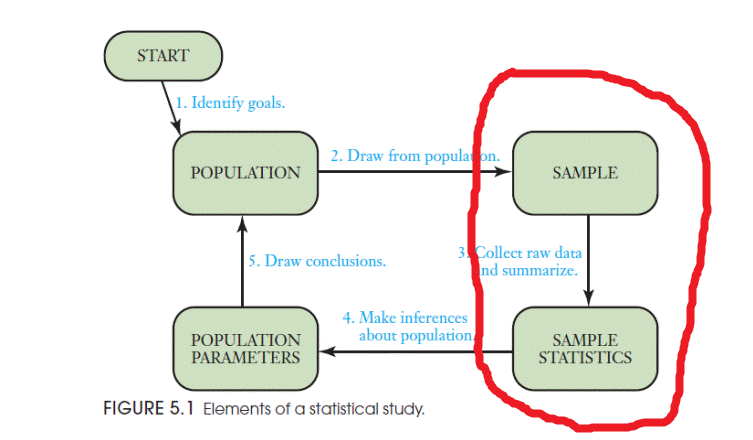
\includegraphics[width=4.16667in,height=\textheight]{images/sample2.png}

\hypertarget{ux442ux438ux43fux44b-ux448ux43aux430ux43b}{%
\section{Типы шкал}\label{ux442ux438ux43fux44b-ux448ux43aux430ux43b}}

Перед тем, как начать речь об описательных статистиках, нужно
разобраться с существующими типами шкал. Типы шкал классифицируются на
основании типа измеряемых данных, которые задают допустимые для данной
шкалы отношения.

\textbf{- Шкала наименований (номинальная шкала)} --- самая простая
шкала, где единственное отношение между элементами --- это отношения
равенства и неравенства. Это любая качественная шкала, между элементами
которой не могут быть установлены отношения ``больше --- меньше''. Это
большинство группирующих переменных (экспериментальная группа, пол,
политическая партия, страна), переменные с id. Еще один пример - номера
на майках у футболистов.

\textbf{- Шкала порядка (ранговая шкала)} --- шкала следующего уровня,
для которой можно установить отношения ``больше --- меньше'', причем
если \emph{B} больше \emph{A}, а \emph{C} больше \emph{B}, то и \emph{C}
должно быть больше \emph{A}. Если это верно, то мы можем выстроить
последовательность значений. Однако мы еще не можем говорить о разнице
между значениями. Ответы на вопросы ``Как часто вы курите?'' по шкале
``Никогда'', ``Редко'' и ``Часто'' являются примером ранговой шкалы.
``Часто'' --- это чаще, чем ``Редко'', ``Редко'' --- это чаще чем
``Никогда'', и, соотвественно, ``Часто'' --- это чаще, чем ``Никогда''.
Но мы не можем сказать, что разница между ``Часто'' и ``Редко'' такая
же, как и между ``Редко'' и ``Никогда''. Соответственно, даже если мы
обозначим ``Часто'', ``Редко'' и ``Никогда'' как 3, 2 и 1
соответственно, то многого не можем сделать с этой шкалой, Например, мы
не можем посчитать арифметическое среднее для такой шкалы.

\textbf{- Шкала разностей (интервальная шкала)} --- шкала, для которой
мы уже можем говорить про разницы между интервалами. Например, разница
между 10 Cº и 20 Cº такая же как и между 80 Cº и 90 Cº. Для шкалы
разностей уже можно сравнивать средние, но операции умножения и деления
не имеют смысл, потому что ноль в шкале разностей относительный.
Например, мы не можем сказать, что 20 Cº --- это в два раза теплее, чем
10 Cº, потому что 0 Cº --- это просто условно взятая точка ---
температура плавления льда.

\textbf{- Шкала отношений (абсолютная шкала)} --- самая ``полноценная''
шкала, которая отличается от интервальной наличием естественного и
однозначного начала координат. Например, масса в килограммах или та же
температура, но в градусах Кельвина, а не Цельсия.

\hypertarget{sec-quantiles}{%
\section{Квантили}\label{sec-quantiles}}

В жизни мы постоянно проходим какие-нибудь тесты, получаем баллы и рано
или поздно встает вопрос: ну а как оно у других? Как бы нас ни учили
книжки по саморазвитию, что не стоит сравнивать себя с другими, от этого
вопроса очень сложно избавиться. А иногда и вовсе не нужно.

Допустим, вы проходите профессиональный тест с задачами одинаковой
сложности. Как понять, если вы решили 10 из 20 задач (допустим, что
задачи одинаковой сложности), то это много или мало? Мы договорились,
что задачи одинаковой сложности, но не сказали какой. Если все 20 задач
очень легкие, то 10 -- это мало, а если сложные -- то много. В этой
ситуации может быть важен относительный успех: сколько людей справились
с тестом хуже вас, а сколько - лучше вас. Вот это и позволяют посчитать
\textbf{процентили} (\emph{percentile rank}) -- процент значений в
распределении ниже заданного значения. То есть 90ый процентиль означает,
что вы справились лучше, чем 90\% людей, который прошли тот же тест. То
есть вы находитесь в 10\% самых-самых! Поэтому настоящие понторезы
должны меряться не абсолютными значениями, а процентилями.

Здесь сразу нужно оговориться, что понятие процентиля имеет несколько
неоднозначностей. В английском принято разделять \emph{percentile} и
\emph{percentile rank}. \emph{Percentile rank} -- это процент значений в
распределении ниже заданного, то просто \emph{percentile} -- это само
значение, ниже которого находится соответствующий процент значений. А
иногда и вовсе процентилем называют сам интервал между процентильными
границами. Все эти понятия взаимосвязаны, поэтому о том, в каком именно
значении используется понятие ``процентиль'' можно догадаться из
контекста. Другая неоднозначность понятия процентиля связана с тем, в
какой процентиль относить пограничные значения. Эта проблема породила
целых девять различных подходов к расчету процентилей! Однако если шкала
континуальная и имеет достаточно много значений, то разницы между этими
подходами не будет.

Можно делить значения не на 100 интервалов, а на меньшее количество.
Например, на 4. Для этого нам нужно три точки: одна отделяет 25\%
наименьших значений, вторая отделяет нижнее 50\% от верхних 50\% (то
есть это медиана!), третья -- верхние 25\% отнижних 75\%. Эти точки и
интервалы, разделяемые ими, называются \textbf{квартилями}.

Кроме процентилей и квартилей есть еще \textbf{децили},
\textbf{квинтили}, \textbf{секстили}, \textbf{септили} и что угодно
\textbf{-тили}, хотя и используются они гораздо реже. Общее название для
всех них -- \textbf{квантили}.

\hypertarget{sec-cent_tend}{%
\section{Меры центральной тенденции}\label{sec-cent_tend}}

Продолжим работать с данными про супергероев.

\begin{Shaded}
\begin{Highlighting}[]
\FunctionTok{library}\NormalTok{(}\StringTok{"tidyverse"}\NormalTok{)}
\end{Highlighting}
\end{Shaded}

\begin{verbatim}
-- Attaching packages --------------------------------------- tidyverse 1.3.2 --
v ggplot2 3.4.2     v purrr   1.0.1
v tibble  3.2.1     v dplyr   1.1.2
v tidyr   1.3.0     v stringr 1.5.0
v readr   2.1.3     v forcats 1.0.0
-- Conflicts ------------------------------------------ tidyverse_conflicts() --
x dplyr::filter() masks stats::filter()
x dplyr::lag()    masks stats::lag()
\end{verbatim}

\begin{Shaded}
\begin{Highlighting}[]
\NormalTok{heroes }\OtherTok{\textless{}{-}} \FunctionTok{read\_csv}\NormalTok{(}\StringTok{"https://raw.githubusercontent.com/Pozdniakov/tidy\_stats/master/data/heroes\_information.csv"}\NormalTok{,}
                   \AttributeTok{na =} \FunctionTok{c}\NormalTok{(}\StringTok{"{-}"}\NormalTok{, }\StringTok{"{-}99"}\NormalTok{))}
\end{Highlighting}
\end{Shaded}

\begin{verbatim}
New names:
* `` -> `...1`
\end{verbatim}

\begin{verbatim}
Warning: One or more parsing issues, call `problems()` on your data frame for details,
e.g.:
  dat <- vroom(...)
  problems(dat)
\end{verbatim}

\begin{verbatim}
Rows: 734 Columns: 11
-- Column specification --------------------------------------------------------
Delimiter: ","
chr (8): name, Gender, Eye color, Race, Hair color, Publisher, Skin color, A...
dbl (3): ...1, Height, Weight

i Use `spec()` to retrieve the full column specification for this data.
i Specify the column types or set `show_col_types = FALSE` to quiet this message.
\end{verbatim}

Для примера мы возьмем массу супергероев, предварительно удалив из нее
все \texttt{NA} для удобства.

\begin{Shaded}
\begin{Highlighting}[]
\NormalTok{weight }\OtherTok{\textless{}{-}}\NormalTok{ heroes }\SpecialCharTok{\%\textgreater{}\%}
  \FunctionTok{drop\_na}\NormalTok{(Weight) }\SpecialCharTok{\%\textgreater{}\%}
  \FunctionTok{pull}\NormalTok{(Weight)}
\end{Highlighting}
\end{Shaded}

Мера центральной тенденции - это число для описания \emph{центра}
распределения.

\hypertarget{sec-mean}{%
\subsection{Арифметическое среднее}\label{sec-mean}}

Самая распространенная мера центральных тенденций -
\textbf{арифметическое среднее}, то самое, которые мы считаем с помощью
функции \texttt{mean()}.

\[\overline{x}= \frac{\sum\limits_{i=1}^{n} x_{i}} {n}\]

Не пугайтесь значка \(\sum\limits_{i=1}^{n}\) -- он означает сумму от
\(i = 1\) до \(n\). Что-то вроде цикла \texttt{for}!

\begin{tcolorbox}[enhanced jigsaw, leftrule=.75mm, toprule=.15mm, left=2mm, breakable, arc=.35mm, rightrule=.15mm, colback=white, opacityback=0, bottomrule=.15mm]

\textbf{\emph{Практика:} функция \emph{my\_mean()}}\vspace{2mm}

В качестве упражнения попробуйте самостоятельно превратить эту формулу в
функцию \texttt{mymean()} c помощью \texttt{sum()} и \texttt{length()}.
Можете убирать \texttt{NA} по дефолту! Сравните с результатом функции
\texttt{mean()}.

\begin{Shaded}
\begin{Highlighting}[]
\FunctionTok{mean}\NormalTok{(weight)}
\end{Highlighting}
\end{Shaded}

\begin{verbatim}
[1] 112.2525
\end{verbatim}

\end{tcolorbox}

\hypertarget{sec-median}{%
\subsection{Медиана}\label{sec-median}}

Представьте себе, что мы считаем среднюю зарплату сотрудников завода.
Большинство рабочих получает 30000-40000 рублей в месяц, а директор
завода получает 2 миллиона в месяц. Средняя зарплата на заводе в итоге
равна 70000 рублей. Никакого подвоха: мы просто применили арифметическое
среднее. Что спросили, то и получили, никаких манипуляций с цифрами! На
деле же нас интересует обычно не средняя зарплата, а сколько получает
средний сотрудник. Не директор, не главный мастер, но и не новичок и не
алкоголик Василий, который постоянно опаздывает и плохо справляется с
работой. Простой рабочий Иван, нормальный парень. Сколько зарабатывают
такие как он? Для ответа на этот вопрос используют не арифметическое
среднее, а \textbf{медиану.}

\textbf{Медиана (median)} - это \emph{середина} распределения.
Представим, что мы расставили значения по порядку (от меньшего к
большему) и взяли значение посередине.

Если у нас четное количество значений, то берется среднее значение между
теми двумя, что по середине.

Для расчета медианы есть функция \texttt{median()}:

\begin{Shaded}
\begin{Highlighting}[]
\FunctionTok{median}\NormalTok{(weight)}
\end{Highlighting}
\end{Shaded}

\begin{verbatim}
[1] 81
\end{verbatim}

Разница медианы со средним существенная. Это значит, что распределение
довольно асимметричное.

Представьте себе, что кто-то говорит про среднюю зарплату в Москве. Но
ведь эта средняя зарплата становится гораздо больше, если учитывать
относительно небольшое количество мультимиллионеров и миллиардеров! А
вот медианная зарплата будет гораздо меньше.

Представьте себе, что в среде супергероев поялвяется кто-то, кто весит
9000 килограммов! Тогда среднее сильно изменится:

\begin{Shaded}
\begin{Highlighting}[]
\FunctionTok{mean}\NormalTok{(}\FunctionTok{c}\NormalTok{(weight, }\DecValTok{9000}\NormalTok{))}
\end{Highlighting}
\end{Shaded}

\begin{verbatim}
[1] 130.1714
\end{verbatim}

А вот медиана останется той же.

\begin{Shaded}
\begin{Highlighting}[]
\FunctionTok{median}\NormalTok{(}\FunctionTok{c}\NormalTok{(weight, }\DecValTok{9000}\NormalTok{))}
\end{Highlighting}
\end{Shaded}

\begin{verbatim}
[1] 81
\end{verbatim}

Таким образом, экстремально большие или маленькие значения оказывают
сильное влияние на арифметическое среднее, но не на медиану. Поэтому
медиана считается более ``робастной'' оценкой, т.е. более устойчивой к
выбросам и крайним значениям.

\hypertarget{sec-trim}{%
\subsection{Усеченное среднее (trimmed mean)}\label{sec-trim}}

Если про среднее и медиану слышали все, то про усеченное (тримленное)
среднее известно гораздо меньше. Тем не менее, на практике это довольно
удобная штука, потому что представляет собой некий компромисс между
арифметическим средним и медианой.

В усеченном среднем значения ранжируются так же, как и для медианы, но
отбрасывается только какой-то процент крайних значений. Усеченное
среднее можно посчитать с помощью обычной функции \texttt{mean()},
поставив нужное значение параметра \texttt{trim\ =}:

\begin{Shaded}
\begin{Highlighting}[]
\FunctionTok{mean}\NormalTok{(weight, }\AttributeTok{trim =} \FloatTok{0.1}\NormalTok{)}
\end{Highlighting}
\end{Shaded}

\begin{verbatim}
[1] 89.56423
\end{verbatim}

\texttt{trim\ =\ 0.1} означает, что мы отбросили 10\% слева и 10\%
справа. \texttt{trim} может принимать значения от 0 до 0.5. Что будет,
если \texttt{trim\ =\ 0}?

\begin{Shaded}
\begin{Highlighting}[]
\FunctionTok{mean}\NormalTok{(weight, }\AttributeTok{trim =} \DecValTok{0}\NormalTok{)}
\end{Highlighting}
\end{Shaded}

\begin{verbatim}
[1] 112.2525
\end{verbatim}

Обычное арифметическое среднее! А если \texttt{trim\ =\ 0.5}?

\begin{Shaded}
\begin{Highlighting}[]
\FunctionTok{mean}\NormalTok{(weight, }\AttributeTok{trim =} \FloatTok{0.5}\NormalTok{)}
\end{Highlighting}
\end{Shaded}

\begin{verbatim}
[1] 81
\end{verbatim}

Медиана!

\hypertarget{sec-mode}{%
\subsection{Мода}\label{sec-mode}}

\textbf{Мода} \emph{(mode)} - это самое \emph{частое} значение. Обычно
используется для номинальных переменных, для континуальных данных мода
неприменима. Что интересно, в R нет встроенной функции для подсчета
моды. Обычно она и не нужна: мы можем посчитать таблицу частот и даже
проранжировать ее (и мы уже умеем это делать разными способами).

\begin{Shaded}
\begin{Highlighting}[]
\NormalTok{heroes }\SpecialCharTok{\%\textgreater{}\%}
  \FunctionTok{count}\NormalTok{(Gender, }\AttributeTok{sort =} \ConstantTok{TRUE}\NormalTok{)}
\end{Highlighting}
\end{Shaded}

\begin{verbatim}
# A tibble: 3 x 2
  Gender     n
  <chr>  <int>
1 Male     505
2 Female   200
3 <NA>      29
\end{verbatim}

\begin{quote}
Можете попробовать написать свою функцию для моды!
\end{quote}

\hypertarget{sec-vary}{%
\section{Меры рассеяния}\label{sec-vary}}

\begin{quote}
Начинающий статистик пытался перейти в брод реку, средняя глубина
которой 1 метр. И утонул.\\
В чем была его ошибка? Он не учитывал разброс значений глубины!
\end{quote}

Мер центральной тенденции недостаточно, чтобы описать выборку.
Необходимо знать ее вариабельность.\\

\hypertarget{sec-range}{%
\subsection{Размах}\label{sec-range}}

Самое очевидное - посчитать \textbf{размах} \emph{(range)}, то есть
разницу между минимальным и максимальным значением. В R есть функция для
вывода максимального и минимального значений:

\begin{Shaded}
\begin{Highlighting}[]
\FunctionTok{range}\NormalTok{(weight)}
\end{Highlighting}
\end{Shaded}

\begin{verbatim}
[1]   2 900
\end{verbatim}

Осталось посчитать разницу между ними:

\begin{Shaded}
\begin{Highlighting}[]
\FunctionTok{diff}\NormalTok{(}\FunctionTok{range}\NormalTok{(weight))}
\end{Highlighting}
\end{Shaded}

\begin{verbatim}
[1] 898
\end{verbatim}

Естественно, крайние значения очень сильно влияют на этот размах,
поэтому на практике он не очень-то используется.

\hypertarget{sec-var}{%
\subsection{Дисперсия}\label{sec-var}}

\textbf{Дисперсия} \emph{(variance)} вычисляется по следующей формуле:

\[s^2= \frac{\sum\limits_{i=1}^{n} (x_{i} - \overline{x})^2} {n}\]

Попробуйте превратить это в функцию \texttt{myvar()}!

\begin{Shaded}
\begin{Highlighting}[]
\NormalTok{myvar }\OtherTok{\textless{}{-}} \ControlFlowTok{function}\NormalTok{(x) }\FunctionTok{mean}\NormalTok{((x }\SpecialCharTok{{-}} \FunctionTok{mean}\NormalTok{(x))}\SpecialCharTok{\^{}}\DecValTok{2}\NormalTok{)}
\end{Highlighting}
\end{Shaded}

Естественно, в R уже есть готовая функция \texttt{var()}. Но, заметьте,
ее результат немного отличается от нашего:

\begin{Shaded}
\begin{Highlighting}[]
\FunctionTok{myvar}\NormalTok{(weight)}
\end{Highlighting}
\end{Shaded}

\begin{verbatim}
[1] 10825.55
\end{verbatim}

\begin{Shaded}
\begin{Highlighting}[]
\FunctionTok{var}\NormalTok{(weight)}
\end{Highlighting}
\end{Shaded}

\begin{verbatim}
[1] 10847.46
\end{verbatim}

Дело в том, что встроенная функция \texttt{var()} делит не на \(n\), а
на \(n-1\). Это связано с тем, что эта функция пытается оценить
дисперсию в генеральной совокупности, т.е. относится уже к статистике
вывода. Про это мы будем говорить в дальнейших занятиях, сейчас нам
нужно только отметить то, что здесь есть небольшое различие.

\hypertarget{sec-sd}{%
\subsection{Стандартное отклонение}\label{sec-sd}}

Если вы заметили, значение дисперсии очень большое. Чтобы вернуться к
единицам измерения, соответствующих нашим данным используется корень из
дисперсии, то есть \textbf{стандартное отклонение} \emph{(standard
deviation)}:

\[s= \sqrt\frac{\sum\limits_{i=1}^{n} (x_{i} - \overline{x})^2} {n}\]

Для этого есть функция \texttt{sd()}:

\begin{Shaded}
\begin{Highlighting}[]
\FunctionTok{sd}\NormalTok{(weight)}
\end{Highlighting}
\end{Shaded}

\begin{verbatim}
[1] 104.1511
\end{verbatim}

Что то же самое, что и:

\begin{Shaded}
\begin{Highlighting}[]
\FunctionTok{sqrt}\NormalTok{(}\FunctionTok{var}\NormalTok{(weight))}
\end{Highlighting}
\end{Shaded}

\begin{verbatim}
[1] 104.1511
\end{verbatim}

\hypertarget{sec-z_scores}{%
\subsubsection{\texorpdfstring{Преобразование в
\(z\)-оценки}{Преобразование в z-оценки}}\label{sec-z_scores}}

На основе арифметического среднего и стандартного отклонения вычисляются
\(z\)-оценки (\(z\)-scores) по простой формуле:

\[
z_i = \frac{x_i - \overline{x}}{s}
\]

Проще говоря, \(z\)-оценки -- это центрированные вокруг нуля значения в
единицах стандартного отклонения. Это может понадобится в случае
необходимости свести разные шкалы как одной размерности (со средним
равным нулю и стандартным отклонением равным одному).
\(z\)-преобразование является стандартной процедурой для многих методов,
например, для анализа главных компонент (см. \textbf{?@sec-pca}).

Для проведения \(z\)-преобразования можно воспользоваться встроенной
функцией \texttt{scale()}, однако она возвращает \(z\)-оценки в довольно
неочевидном формате: матрицу (см. Глава~\ref{sec-matrix}) с атрибутами
(см. Глава~\ref{sec-attr_class}) \texttt{"scaled:center"} (среднее
изначальной шкалы) и \texttt{"scaled:scale"} (стандартное отклонение
изначальной шкалы). Впрочем, функцию для \(z\)-преобразования легко
написать самостоятельно:

\begin{Shaded}
\begin{Highlighting}[]
\FunctionTok{head}\NormalTok{(}\FunctionTok{scale}\NormalTok{(weight))}
\end{Highlighting}
\end{Shaded}

\begin{verbatim}
            [,1]
[1,]  3.15644618
[2,] -0.45369186
[3,] -0.21365608
[4,]  3.15644618
[5,]  0.09358971
[6,] -0.23285895
\end{verbatim}

\begin{Shaded}
\begin{Highlighting}[]
\NormalTok{z }\OtherTok{\textless{}{-}} \ControlFlowTok{function}\NormalTok{(x) (x }\SpecialCharTok{{-}} \FunctionTok{mean}\NormalTok{(x, }\AttributeTok{na.rm =} \ConstantTok{TRUE}\NormalTok{))}\SpecialCharTok{/}\FunctionTok{sd}\NormalTok{(x, }\AttributeTok{na.rm =} \ConstantTok{TRUE}\NormalTok{)}
\FunctionTok{head}\NormalTok{(}\FunctionTok{z}\NormalTok{(weight))}
\end{Highlighting}
\end{Shaded}

\begin{verbatim}
[1]  3.15644618 -0.45369186 -0.21365608  3.15644618  0.09358971 -0.23285895
\end{verbatim}

\hypertarget{sec-mad}{%
\subsection{Медианное абсолютное отклонение}\label{sec-mad}}

Поскольку стандартное отклонение не устойчиво к выбросам, то иногда
используют его альтернативу, которая устойчива к выбросам (особенно если
эти выбросы нам как раз и нужно удалить) - медианное абсолютное
отклонение (median absolute deviation):

\[mad= median(|x_{i} - median(x)|)\]

Для этого есть функция \texttt{mad()}:

\begin{Shaded}
\begin{Highlighting}[]
\FunctionTok{mad}\NormalTok{(weight)}
\end{Highlighting}
\end{Shaded}

\begin{verbatim}
[1] 32.6172
\end{verbatim}

\hypertarget{sec-iqr}{%
\subsection{Межквартильный размах}\label{sec-iqr}}

Другой вариант рабостной оценки вариабельности данных является
\textbf{межквартильный размах} \emph{(interquartile range, IQR)}. Это
разница между третьим и первым \textbf{квартилем} \footnote{Квартиль ---
  это частный пример квантиля. Другой известный квантиль --- процентиль.
  Процентили часто используют для сравнения значения с другими
  значениями. Например, 63ий процентиль означает, что данное значение
  больше 63\% значений в выборке.} - значением, которое больше 75\%
значений в выборке, и значением, которое больше 25\% значений в выборке.

\begin{Shaded}
\begin{Highlighting}[]
\FunctionTok{IQR}\NormalTok{(weight)}
\end{Highlighting}
\end{Shaded}

\begin{verbatim}
[1] 47
\end{verbatim}

\begin{quote}
Ну а второй квартиль - это медиана!
\end{quote}

\hypertarget{sec-skku}{%
\section{Асимметрия и эксцесс}\label{sec-skku}}

\hypertarget{sec-skew}{%
\subsection{Асимметрия}\label{sec-skew}}

\textbf{Асимметрия \emph{(skewness)}} измеряет симметричность
распределения. \textbf{Положительный показатель асимметрии}
\textbf{\emph{(``Right-skewed''}} или \textbf{\emph{positive skewness)}}
означает, что хвосты с правой части распределения длиннее.
\textbf{Негативный показатель асимметрии (\emph{``Left-skewed''}} или
\textbf{\emph{negative skewness)}} означает, что левый хвост длиннее.
Нулевой показатель асимметрии означает симметричное распределение.

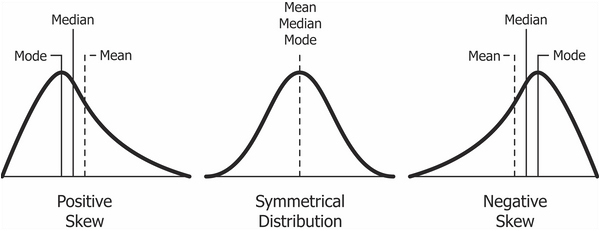
\includegraphics[width=4.16667in,height=\textheight]{images/7180OS_01_180.jpg}

В целом, распределения с положительным показателем асимметрии на
практике встречаются чаще, чем с отрицательным: очень часто мы
сталкиваемся со шкалами, которые ограничены снизу, но не ограничены
сверху.

\begin{itemize}
\item
  В когнитивистике положительная асимметрия встречается очень часто.
  Например, время реакции: оно ограничено снизу 0 мс (а по факту не
  меньше 100 мс -- быстрее сигнал не успеет по нервной системе пройти до
  пальцев), а вот с другой стороны оно никак не ограничено. Испытуемый
  может на полчаса перед монитором затупить, ага.
\item
  Если мы анализируем размеры индивидуальные доходы, то они не могут
  быть меньше 0, но могут быть невероятно большими для относительно
  небольшого количества миллионеров и миллиардеров. Доходы остальных
  людей находятся в относительно небольшом диапазоне (который гораздо
  ближе к нулю, чем к доходам миллиардеров)
\end{itemize}

\hypertarget{sec-kurtosis}{%
\subsection{Эксцесс}\label{sec-kurtosis}}

\textbf{Эксцесс \emph{(kurtosis)}} - это мера ``вытянутости''
распределения:

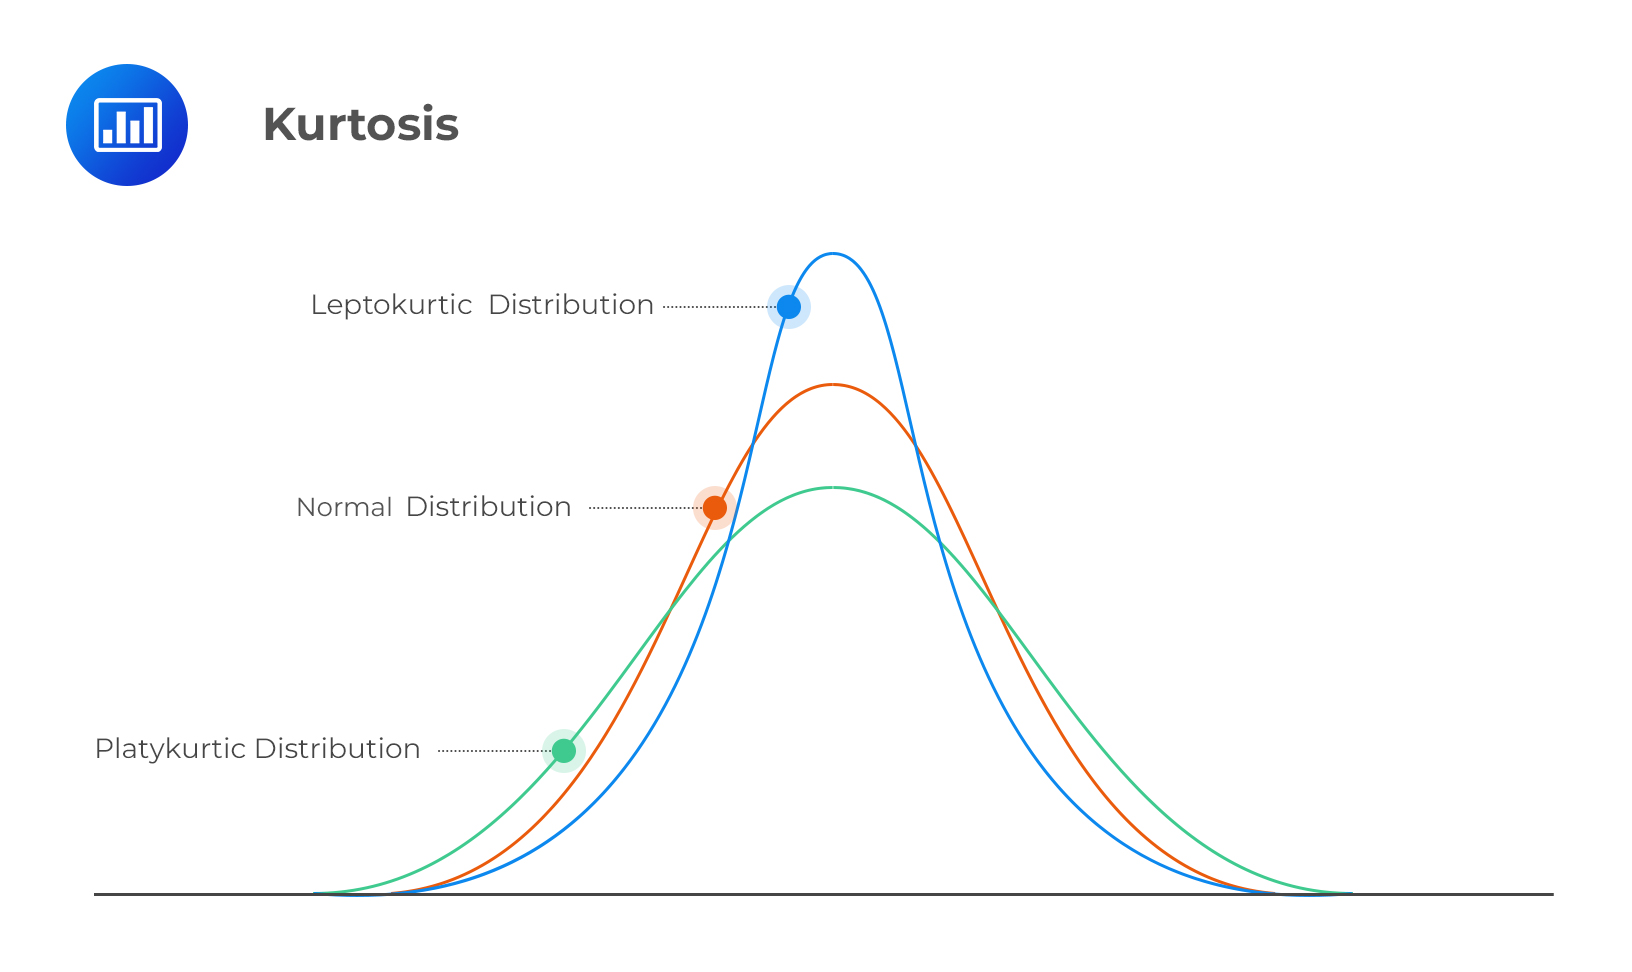
\includegraphics{images/page-64.png}

Положительные показатели эксцесса означают ``вытянутое'' распределение,
а отрицательные - ``плоское''.

\hypertarget{sec-skewR}{%
\subsection{Ассиметрия и эксцесс в R}\label{sec-skewR}}

К сожалению, в базовом R нет функций для асимметрии и эксцесса. Зато
есть замечательный пакет \texttt{\{psych\}} (да-да, специально для
психологов).

\begin{Shaded}
\begin{Highlighting}[]
\FunctionTok{install.packages}\NormalTok{(}\StringTok{"psych"}\NormalTok{)}
\end{Highlighting}
\end{Shaded}

\begin{Shaded}
\begin{Highlighting}[]
\FunctionTok{library}\NormalTok{(}\StringTok{"psych"}\NormalTok{)}
\end{Highlighting}
\end{Shaded}

\begin{verbatim}

Attaching package: 'psych'
\end{verbatim}

\begin{verbatim}
The following objects are masked from 'package:ggplot2':

    %+%, alpha
\end{verbatim}

В нем есть функции \texttt{skew()} и \texttt{kurtosi()}:

\begin{Shaded}
\begin{Highlighting}[]
\FunctionTok{skew}\NormalTok{(weight)}
\end{Highlighting}
\end{Shaded}

\begin{verbatim}
[1] 3.874557
\end{verbatim}

\begin{Shaded}
\begin{Highlighting}[]
\FunctionTok{kurtosi}\NormalTok{(weight)}
\end{Highlighting}
\end{Shaded}

\begin{verbatim}
[1] 19.45699
\end{verbatim}

Асимметрия положительная, это значит что распределение выборки
асимметричное, хвосты с правой части длиннее. Эксцесс значительно выше
нуля - значит распределение довольно ``вытянутое''.

\hypertarget{sec-summary}{%
\section{А теперь все вместе!}\label{sec-summary}}

В базовом R есть функция \texttt{summary()}, которая позволяет получить
сразу неплохой набор описательных статистик.

\begin{Shaded}
\begin{Highlighting}[]
\FunctionTok{summary}\NormalTok{(weight)}
\end{Highlighting}
\end{Shaded}

\begin{verbatim}
   Min. 1st Qu.  Median    Mean 3rd Qu.    Max. 
    2.0    61.0    81.0   112.3   108.0   900.0 
\end{verbatim}

Функция \texttt{summary()} - это \textbf{универсальная \emph{(generic)}}
функция (см. Глава~\ref{sec-attr_class}). Это означает, что Вы можете ее
применять для разных объектов и получать разные результаты. Попробуйте
применить ее к векторам с разными типами данных и даже к датафреймам.
Посмотрите, что получится.

В пакете \texttt{psych} есть еще и замечательная функция
\texttt{describe()}, которая даст Вам еще больше статистик, включая
ассиметрию и куртозис:

\begin{Shaded}
\begin{Highlighting}[]
\NormalTok{psych}\SpecialCharTok{::}\FunctionTok{describe}\NormalTok{(weight)}
\end{Highlighting}
\end{Shaded}

\begin{verbatim}
   vars   n   mean     sd median trimmed   mad min max range skew kurtosis   se
X1    1 495 112.25 104.15     81   89.56 32.62   2 900   898 3.87    19.46 4.68
\end{verbatim}

Даже \textbf{усеченное \emph{(trimmed)} среднее} есть (с
\texttt{trim\ =\ 0.1})! Все кроме \texttt{se} мы уже знаем. А про этот
\texttt{se} узнаем немного позже (см. Глава~\ref{sec-sample_dist}).

Эта функция хорошо работает в сочетании с \texttt{group\_by()}:

\begin{Shaded}
\begin{Highlighting}[]
\NormalTok{heroes }\SpecialCharTok{\%\textgreater{}\%}
  \FunctionTok{group\_by}\NormalTok{(Gender) }\SpecialCharTok{\%\textgreater{}\%}
  \FunctionTok{summarise}\NormalTok{(}\FunctionTok{describe}\NormalTok{(Weight))}
\end{Highlighting}
\end{Shaded}

\begin{verbatim}
# A tibble: 3 x 14
  Gender  vars     n  mean    sd median trimmed   mad   min   max range  skew
  <chr>  <dbl> <dbl> <dbl> <dbl>  <dbl>   <dbl> <dbl> <dbl> <dbl> <dbl> <dbl>
1 Female     1   142  78.8  77.0     58    60.9  7.41    41   630   589  4.97
2 Male       1   339 126.  111.      90   103.  23.7      2   900   898  3.76
3 <NA>       1    14 129.  107.      94   115.  43.0     39   383   344  1.55
# i 2 more variables: kurtosis <dbl>, se <dbl>
\end{verbatim}

Другой интересный пакет для получения описательных статистик для всего
датафрейма --- \texttt{\{skimr\}}.

\begin{Shaded}
\begin{Highlighting}[]
\FunctionTok{install.packages}\NormalTok{(}\StringTok{"skimr"}\NormalTok{)}
\end{Highlighting}
\end{Shaded}

Его основная функция --- \texttt{skim()}, выводит в консоли симпатичную
сводную таблицу:

\begin{Shaded}
\begin{Highlighting}[]
\NormalTok{skimr}\SpecialCharTok{::}\FunctionTok{skim}\NormalTok{(heroes)}
\end{Highlighting}
\end{Shaded}

\begin{longtable}[]{@{}ll@{}}
\caption{Data summary}\tabularnewline
\toprule()
\endhead
Name & heroes \\
Number of rows & 734 \\
Number of columns & 11 \\
\_\_\_\_\_\_\_\_\_\_\_\_\_\_\_\_\_\_\_\_\_\_\_ & \\
Column type frequency: & \\
character & 8 \\
numeric & 3 \\
\_\_\_\_\_\_\_\_\_\_\_\_\_\_\_\_\_\_\_\_\_\_\_\_ & \\
Group variables & None \\
\bottomrule()
\end{longtable}

\textbf{Variable type: character}

\begin{longtable}[]{@{}
  >{\raggedright\arraybackslash}p{(\columnwidth - 14\tabcolsep) * \real{0.1944}}
  >{\raggedleft\arraybackslash}p{(\columnwidth - 14\tabcolsep) * \real{0.1389}}
  >{\raggedleft\arraybackslash}p{(\columnwidth - 14\tabcolsep) * \real{0.1944}}
  >{\raggedleft\arraybackslash}p{(\columnwidth - 14\tabcolsep) * \real{0.0556}}
  >{\raggedleft\arraybackslash}p{(\columnwidth - 14\tabcolsep) * \real{0.0556}}
  >{\raggedleft\arraybackslash}p{(\columnwidth - 14\tabcolsep) * \real{0.0833}}
  >{\raggedleft\arraybackslash}p{(\columnwidth - 14\tabcolsep) * \real{0.1250}}
  >{\raggedleft\arraybackslash}p{(\columnwidth - 14\tabcolsep) * \real{0.1528}}@{}}
\toprule()
\begin{minipage}[b]{\linewidth}\raggedright
skim\_variable
\end{minipage} & \begin{minipage}[b]{\linewidth}\raggedleft
n\_missing
\end{minipage} & \begin{minipage}[b]{\linewidth}\raggedleft
complete\_rate
\end{minipage} & \begin{minipage}[b]{\linewidth}\raggedleft
min
\end{minipage} & \begin{minipage}[b]{\linewidth}\raggedleft
max
\end{minipage} & \begin{minipage}[b]{\linewidth}\raggedleft
empty
\end{minipage} & \begin{minipage}[b]{\linewidth}\raggedleft
n\_unique
\end{minipage} & \begin{minipage}[b]{\linewidth}\raggedleft
whitespace
\end{minipage} \\
\midrule()
\endhead
name & 0 & 1.00 & 1 & 25 & 0 & 715 & 0 \\
Gender & 29 & 0.96 & 4 & 6 & 0 & 2 & 0 \\
Eye color & 172 & 0.77 & 3 & 23 & 0 & 22 & 0 \\
Race & 304 & 0.59 & 5 & 18 & 0 & 61 & 0 \\
Hair color & 172 & 0.77 & 3 & 16 & 0 & 29 & 0 \\
Publisher & 0 & 1.00 & 0 & 17 & 15 & 25 & 0 \\
Skin color & 662 & 0.10 & 3 & 14 & 0 & 16 & 0 \\
Alignment & 7 & 0.99 & 3 & 7 & 0 & 3 & 0 \\
\bottomrule()
\end{longtable}

\textbf{Variable type: numeric}

\begin{longtable}[]{@{}
  >{\raggedright\arraybackslash}p{(\columnwidth - 20\tabcolsep) * \real{0.1591}}
  >{\raggedleft\arraybackslash}p{(\columnwidth - 20\tabcolsep) * \real{0.1136}}
  >{\raggedleft\arraybackslash}p{(\columnwidth - 20\tabcolsep) * \real{0.1591}}
  >{\raggedleft\arraybackslash}p{(\columnwidth - 20\tabcolsep) * \real{0.0795}}
  >{\raggedleft\arraybackslash}p{(\columnwidth - 20\tabcolsep) * \real{0.0795}}
  >{\raggedleft\arraybackslash}p{(\columnwidth - 20\tabcolsep) * \real{0.0568}}
  >{\raggedleft\arraybackslash}p{(\columnwidth - 20\tabcolsep) * \real{0.0795}}
  >{\raggedleft\arraybackslash}p{(\columnwidth - 20\tabcolsep) * \real{0.0682}}
  >{\raggedleft\arraybackslash}p{(\columnwidth - 20\tabcolsep) * \real{0.0795}}
  >{\raggedleft\arraybackslash}p{(\columnwidth - 20\tabcolsep) * \real{0.0568}}
  >{\raggedright\arraybackslash}p{(\columnwidth - 20\tabcolsep) * \real{0.0682}}@{}}
\toprule()
\begin{minipage}[b]{\linewidth}\raggedright
skim\_variable
\end{minipage} & \begin{minipage}[b]{\linewidth}\raggedleft
n\_missing
\end{minipage} & \begin{minipage}[b]{\linewidth}\raggedleft
complete\_rate
\end{minipage} & \begin{minipage}[b]{\linewidth}\raggedleft
mean
\end{minipage} & \begin{minipage}[b]{\linewidth}\raggedleft
sd
\end{minipage} & \begin{minipage}[b]{\linewidth}\raggedleft
p0
\end{minipage} & \begin{minipage}[b]{\linewidth}\raggedleft
p25
\end{minipage} & \begin{minipage}[b]{\linewidth}\raggedleft
p50
\end{minipage} & \begin{minipage}[b]{\linewidth}\raggedleft
p75
\end{minipage} & \begin{minipage}[b]{\linewidth}\raggedleft
p100
\end{minipage} & \begin{minipage}[b]{\linewidth}\raggedright
hist
\end{minipage} \\
\midrule()
\endhead
\ldots1 & 0 & 1.00 & 366.50 & 212.03 & 0.0 & 183.25 & 366.5 & 549.75 &
733 & ▇▇▇▇▇ \\
Height & 217 & 0.70 & 186.73 & 59.25 & 15.2 & 173.00 & 183.0 & 191.00 &
975 & ▇▁▁▁▁ \\
Weight & 239 & 0.67 & 112.25 & 104.15 & 2.0 & 61.00 & 81.0 & 108.00 &
900 & ▇▁▁▁▁ \\
\bottomrule()
\end{longtable}

В зависимости от типа данных колонки функция skim() показывает различные
статистики. Для числовых колонок мы можем увидеть количество и долю
пропущенных значений, среднее и стандартное отклонение. А еще мы видим
некие \emph{p0, p25, p50, p75} и \emph{p100.} Это процентили! И совсем
не с потолка взятые:

\begin{itemize}
\item
  p0 -- минимальное значение,
\item
  p25 -- первый квартиль (Q1),
\item
  p50 -- второй квартиль (Q2), т.е. медиана,
\item
  p75 -- третий квартиль (Q3),
\item
  p100 -- максимальное значение.
\end{itemize}

Ну и вишенкой на торте выступает маленькая гистограмма (см. для каждой
колонки!

Кроме того, \texttt{skimr} адаптирован под tidyverse. В нем можно
выбирать колонки с помощью tidyselect (@ref(tidyselect)) прямо внутри
функции \texttt{skim()}.

\begin{Shaded}
\begin{Highlighting}[]
\NormalTok{heroes }\SpecialCharTok{\%\textgreater{}\%}
\NormalTok{  skimr}\SpecialCharTok{::}\FunctionTok{skim}\NormalTok{(}\FunctionTok{ends\_with}\NormalTok{(}\StringTok{"color"}\NormalTok{))}
\end{Highlighting}
\end{Shaded}

\begin{longtable}[]{@{}ll@{}}
\caption{Data summary}\tabularnewline
\toprule()
\endhead
Name & Piped data \\
Number of rows & 734 \\
Number of columns & 11 \\
\_\_\_\_\_\_\_\_\_\_\_\_\_\_\_\_\_\_\_\_\_\_\_ & \\
Column type frequency: & \\
character & 3 \\
\_\_\_\_\_\_\_\_\_\_\_\_\_\_\_\_\_\_\_\_\_\_\_\_ & \\
Group variables & None \\
\bottomrule()
\end{longtable}

\textbf{Variable type: character}

\begin{longtable}[]{@{}
  >{\raggedright\arraybackslash}p{(\columnwidth - 14\tabcolsep) * \real{0.1944}}
  >{\raggedleft\arraybackslash}p{(\columnwidth - 14\tabcolsep) * \real{0.1389}}
  >{\raggedleft\arraybackslash}p{(\columnwidth - 14\tabcolsep) * \real{0.1944}}
  >{\raggedleft\arraybackslash}p{(\columnwidth - 14\tabcolsep) * \real{0.0556}}
  >{\raggedleft\arraybackslash}p{(\columnwidth - 14\tabcolsep) * \real{0.0556}}
  >{\raggedleft\arraybackslash}p{(\columnwidth - 14\tabcolsep) * \real{0.0833}}
  >{\raggedleft\arraybackslash}p{(\columnwidth - 14\tabcolsep) * \real{0.1250}}
  >{\raggedleft\arraybackslash}p{(\columnwidth - 14\tabcolsep) * \real{0.1528}}@{}}
\toprule()
\begin{minipage}[b]{\linewidth}\raggedright
skim\_variable
\end{minipage} & \begin{minipage}[b]{\linewidth}\raggedleft
n\_missing
\end{minipage} & \begin{minipage}[b]{\linewidth}\raggedleft
complete\_rate
\end{minipage} & \begin{minipage}[b]{\linewidth}\raggedleft
min
\end{minipage} & \begin{minipage}[b]{\linewidth}\raggedleft
max
\end{minipage} & \begin{minipage}[b]{\linewidth}\raggedleft
empty
\end{minipage} & \begin{minipage}[b]{\linewidth}\raggedleft
n\_unique
\end{minipage} & \begin{minipage}[b]{\linewidth}\raggedleft
whitespace
\end{minipage} \\
\midrule()
\endhead
Eye color & 172 & 0.77 & 3 & 23 & 0 & 22 & 0 \\
Hair color & 172 & 0.77 & 3 & 16 & 0 & 29 & 0 \\
Skin color & 662 & 0.10 & 3 & 14 & 0 & 16 & 0 \\
\bottomrule()
\end{longtable}

А еще можно сочетать с группировкой с помощью \texttt{group\_by()}.

\begin{Shaded}
\begin{Highlighting}[]
\NormalTok{heroes }\SpecialCharTok{\%\textgreater{}\%}
  \FunctionTok{group\_by}\NormalTok{(Gender) }\SpecialCharTok{\%\textgreater{}\%}
\NormalTok{  skimr}\SpecialCharTok{::}\FunctionTok{skim}\NormalTok{(}\FunctionTok{ends\_with}\NormalTok{(}\StringTok{"color"}\NormalTok{))}
\end{Highlighting}
\end{Shaded}

\begin{longtable}[]{@{}ll@{}}
\caption{Data summary}\tabularnewline
\toprule()
\endhead
Name & Piped data \\
Number of rows & 734 \\
Number of columns & 11 \\
\_\_\_\_\_\_\_\_\_\_\_\_\_\_\_\_\_\_\_\_\_\_\_ & \\
Column type frequency: & \\
character & 3 \\
\_\_\_\_\_\_\_\_\_\_\_\_\_\_\_\_\_\_\_\_\_\_\_\_ & \\
Group variables & Gender \\
\bottomrule()
\end{longtable}

\textbf{Variable type: character}

\begin{longtable}[]{@{}
  >{\raggedright\arraybackslash}p{(\columnwidth - 16\tabcolsep) * \real{0.1772}}
  >{\raggedright\arraybackslash}p{(\columnwidth - 16\tabcolsep) * \real{0.0886}}
  >{\raggedleft\arraybackslash}p{(\columnwidth - 16\tabcolsep) * \real{0.1266}}
  >{\raggedleft\arraybackslash}p{(\columnwidth - 16\tabcolsep) * \real{0.1772}}
  >{\raggedleft\arraybackslash}p{(\columnwidth - 16\tabcolsep) * \real{0.0506}}
  >{\raggedleft\arraybackslash}p{(\columnwidth - 16\tabcolsep) * \real{0.0506}}
  >{\raggedleft\arraybackslash}p{(\columnwidth - 16\tabcolsep) * \real{0.0759}}
  >{\raggedleft\arraybackslash}p{(\columnwidth - 16\tabcolsep) * \real{0.1139}}
  >{\raggedleft\arraybackslash}p{(\columnwidth - 16\tabcolsep) * \real{0.1392}}@{}}
\toprule()
\begin{minipage}[b]{\linewidth}\raggedright
skim\_variable
\end{minipage} & \begin{minipage}[b]{\linewidth}\raggedright
Gender
\end{minipage} & \begin{minipage}[b]{\linewidth}\raggedleft
n\_missing
\end{minipage} & \begin{minipage}[b]{\linewidth}\raggedleft
complete\_rate
\end{minipage} & \begin{minipage}[b]{\linewidth}\raggedleft
min
\end{minipage} & \begin{minipage}[b]{\linewidth}\raggedleft
max
\end{minipage} & \begin{minipage}[b]{\linewidth}\raggedleft
empty
\end{minipage} & \begin{minipage}[b]{\linewidth}\raggedleft
n\_unique
\end{minipage} & \begin{minipage}[b]{\linewidth}\raggedleft
whitespace
\end{minipage} \\
\midrule()
\endhead
Eye color & Female & 41 & 0.80 & 3 & 23 & 0 & 14 & 0 \\
Eye color & Male & 121 & 0.76 & 3 & 12 & 0 & 18 & 0 \\
Eye color & NA & 10 & 0.66 & 3 & 23 & 0 & 7 & 0 \\
Hair color & Female & 38 & 0.81 & 3 & 16 & 0 & 18 & 0 \\
Hair color & Male & 123 & 0.76 & 3 & 16 & 0 & 23 & 0 \\
Hair color & NA & 11 & 0.62 & 4 & 14 & 0 & 10 & 0 \\
Skin color & Female & 186 & 0.07 & 4 & 6 & 0 & 7 & 0 \\
Skin color & Male & 449 & 0.11 & 3 & 14 & 0 & 14 & 0 \\
Skin color & NA & 27 & 0.07 & 4 & 4 & 0 & 2 & 0 \\
\bottomrule()
\end{longtable}

\hypertarget{ux43eux43fux438ux441ux430ux442ux435ux43bux44cux43dux44bux445-ux441ux442ux430ux442ux438ux441ux442ux438ux43a-ux43dux435ux434ux43eux441ux442ux430ux442ux43eux447ux43dux43e-sec-datasaurus}{%
\subsection{Описательных статистик недостаточно
\{@sec-datasaurus\}}\label{ux43eux43fux438ux441ux430ux442ux435ux43bux44cux43dux44bux445-ux441ux442ux430ux442ux438ux441ux442ux438ux43a-ux43dux435ux434ux43eux441ux442ux430ux442ux43eux447ux43dux43e-sec-datasaurus}}

Я в тайне от Вас загрузил данные в переменную \texttt{xxx} (можете найти
этот набор данных
\href{https://raw.githubusercontent.com/Pozdniakov/stats/master/data/d.csv}{здесь},
если интересно). Выглядят они примерно так:

\begin{Shaded}
\begin{Highlighting}[]
\FunctionTok{head}\NormalTok{(xxx)}
\end{Highlighting}
\end{Shaded}

\begin{verbatim}
# A tibble: 6 x 2
      x     y
  <dbl> <dbl>
1  55.4  97.2
2  51.5  96.0
3  46.2  94.5
4  42.8  91.4
5  40.8  88.3
6  38.7  84.9
\end{verbatim}

\begin{Shaded}
\begin{Highlighting}[]
\FunctionTok{str}\NormalTok{(xxx)}
\end{Highlighting}
\end{Shaded}

\begin{verbatim}
spc_tbl_ [142 x 2] (S3: spec_tbl_df/tbl_df/tbl/data.frame)
 $ x: num [1:142] 55.4 51.5 46.2 42.8 40.8 ...
 $ y: num [1:142] 97.2 96 94.5 91.4 88.3 ...
 - attr(*, "spec")=
  .. cols(
  ..   x = col_double(),
  ..   y = col_double()
  .. )
 - attr(*, "problems")=<externalptr> 
\end{verbatim}

Надеюсь, Вы уже понимаете, как это интерпретировать - два столбца с 142
числами каждый. Представьте себе, как выглядят эти точки на плоскости,
если каждая строчка означают координаты одной точки по осям \emph{x} и
\emph{y} (это называется диаграмма рассеяния, точечная диаграмма или
scatterplot).

\begin{verbatim}
Warning in grid.Call(C_textBounds, as.graphicsAnnot(x$label), x$x, x$y, :
conversion failure on 'Представьте точки здесь:' in 'mbcsToSbcs': dot
substituted for <d0>
\end{verbatim}

\begin{verbatim}
Warning in grid.Call(C_textBounds, as.graphicsAnnot(x$label), x$x, x$y, :
conversion failure on 'Представьте точки здесь:' in 'mbcsToSbcs': dot
substituted for <9f>
\end{verbatim}

\begin{verbatim}
Warning in grid.Call(C_textBounds, as.graphicsAnnot(x$label), x$x, x$y, :
conversion failure on 'Представьте точки здесь:' in 'mbcsToSbcs': dot
substituted for <d1>
\end{verbatim}

\begin{verbatim}
Warning in grid.Call(C_textBounds, as.graphicsAnnot(x$label), x$x, x$y, :
conversion failure on 'Представьте точки здесь:' in 'mbcsToSbcs': dot
substituted for <80>
\end{verbatim}

\begin{verbatim}
Warning in grid.Call(C_textBounds, as.graphicsAnnot(x$label), x$x, x$y, :
conversion failure on 'Представьте точки здесь:' in 'mbcsToSbcs': dot
substituted for <d0>
\end{verbatim}

\begin{verbatim}
Warning in grid.Call(C_textBounds, as.graphicsAnnot(x$label), x$x, x$y, :
conversion failure on 'Представьте точки здесь:' in 'mbcsToSbcs': dot
substituted for <b5>
\end{verbatim}

\begin{verbatim}
Warning in grid.Call(C_textBounds, as.graphicsAnnot(x$label), x$x, x$y, :
conversion failure on 'Представьте точки здесь:' in 'mbcsToSbcs': dot
substituted for <d0>
\end{verbatim}

\begin{verbatim}
Warning in grid.Call(C_textBounds, as.graphicsAnnot(x$label), x$x, x$y, :
conversion failure on 'Представьте точки здесь:' in 'mbcsToSbcs': dot
substituted for <b4>
\end{verbatim}

\begin{verbatim}
Warning in grid.Call(C_textBounds, as.graphicsAnnot(x$label), x$x, x$y, :
conversion failure on 'Представьте точки здесь:' in 'mbcsToSbcs': dot
substituted for <d1>
\end{verbatim}

\begin{verbatim}
Warning in grid.Call(C_textBounds, as.graphicsAnnot(x$label), x$x, x$y, :
conversion failure on 'Представьте точки здесь:' in 'mbcsToSbcs': dot
substituted for <81>
\end{verbatim}

\begin{verbatim}
Warning in grid.Call(C_textBounds, as.graphicsAnnot(x$label), x$x, x$y, :
conversion failure on 'Представьте точки здесь:' in 'mbcsToSbcs': dot
substituted for <d1>
\end{verbatim}

\begin{verbatim}
Warning in grid.Call(C_textBounds, as.graphicsAnnot(x$label), x$x, x$y, :
conversion failure on 'Представьте точки здесь:' in 'mbcsToSbcs': dot
substituted for <82>
\end{verbatim}

\begin{verbatim}
Warning in grid.Call(C_textBounds, as.graphicsAnnot(x$label), x$x, x$y, :
conversion failure on 'Представьте точки здесь:' in 'mbcsToSbcs': dot
substituted for <d0>
\end{verbatim}

\begin{verbatim}
Warning in grid.Call(C_textBounds, as.graphicsAnnot(x$label), x$x, x$y, :
conversion failure on 'Представьте точки здесь:' in 'mbcsToSbcs': dot
substituted for <b0>
\end{verbatim}

\begin{verbatim}
Warning in grid.Call(C_textBounds, as.graphicsAnnot(x$label), x$x, x$y, :
conversion failure on 'Представьте точки здесь:' in 'mbcsToSbcs': dot
substituted for <d0>
\end{verbatim}

\begin{verbatim}
Warning in grid.Call(C_textBounds, as.graphicsAnnot(x$label), x$x, x$y, :
conversion failure on 'Представьте точки здесь:' in 'mbcsToSbcs': dot
substituted for <b2>
\end{verbatim}

\begin{verbatim}
Warning in grid.Call(C_textBounds, as.graphicsAnnot(x$label), x$x, x$y, :
conversion failure on 'Представьте точки здесь:' in 'mbcsToSbcs': dot
substituted for <d1>
\end{verbatim}

\begin{verbatim}
Warning in grid.Call(C_textBounds, as.graphicsAnnot(x$label), x$x, x$y, :
conversion failure on 'Представьте точки здесь:' in 'mbcsToSbcs': dot
substituted for <8c>
\end{verbatim}

\begin{verbatim}
Warning in grid.Call(C_textBounds, as.graphicsAnnot(x$label), x$x, x$y, :
conversion failure on 'Представьте точки здесь:' in 'mbcsToSbcs': dot
substituted for <d1>
\end{verbatim}

\begin{verbatim}
Warning in grid.Call(C_textBounds, as.graphicsAnnot(x$label), x$x, x$y, :
conversion failure on 'Представьте точки здесь:' in 'mbcsToSbcs': dot
substituted for <82>
\end{verbatim}

\begin{verbatim}
Warning in grid.Call(C_textBounds, as.graphicsAnnot(x$label), x$x, x$y, :
conversion failure on 'Представьте точки здесь:' in 'mbcsToSbcs': dot
substituted for <d0>
\end{verbatim}

\begin{verbatim}
Warning in grid.Call(C_textBounds, as.graphicsAnnot(x$label), x$x, x$y, :
conversion failure on 'Представьте точки здесь:' in 'mbcsToSbcs': dot
substituted for <b5>
\end{verbatim}

\begin{verbatim}
Warning in grid.Call(C_textBounds, as.graphicsAnnot(x$label), x$x, x$y, :
conversion failure on 'Представьте точки здесь:' in 'mbcsToSbcs': dot
substituted for <d1>
\end{verbatim}

\begin{verbatim}
Warning in grid.Call(C_textBounds, as.graphicsAnnot(x$label), x$x, x$y, :
conversion failure on 'Представьте точки здесь:' in 'mbcsToSbcs': dot
substituted for <82>
\end{verbatim}

\begin{verbatim}
Warning in grid.Call(C_textBounds, as.graphicsAnnot(x$label), x$x, x$y, :
conversion failure on 'Представьте точки здесь:' in 'mbcsToSbcs': dot
substituted for <d0>
\end{verbatim}

\begin{verbatim}
Warning in grid.Call(C_textBounds, as.graphicsAnnot(x$label), x$x, x$y, :
conversion failure on 'Представьте точки здесь:' in 'mbcsToSbcs': dot
substituted for <be>
\end{verbatim}

\begin{verbatim}
Warning in grid.Call(C_textBounds, as.graphicsAnnot(x$label), x$x, x$y, :
conversion failure on 'Представьте точки здесь:' in 'mbcsToSbcs': dot
substituted for <d1>
\end{verbatim}

\begin{verbatim}
Warning in grid.Call(C_textBounds, as.graphicsAnnot(x$label), x$x, x$y, :
conversion failure on 'Представьте точки здесь:' in 'mbcsToSbcs': dot
substituted for <87>
\end{verbatim}

\begin{verbatim}
Warning in grid.Call(C_textBounds, as.graphicsAnnot(x$label), x$x, x$y, :
conversion failure on 'Представьте точки здесь:' in 'mbcsToSbcs': dot
substituted for <d0>
\end{verbatim}

\begin{verbatim}
Warning in grid.Call(C_textBounds, as.graphicsAnnot(x$label), x$x, x$y, :
conversion failure on 'Представьте точки здесь:' in 'mbcsToSbcs': dot
substituted for <ba>
\end{verbatim}

\begin{verbatim}
Warning in grid.Call(C_textBounds, as.graphicsAnnot(x$label), x$x, x$y, :
conversion failure on 'Представьте точки здесь:' in 'mbcsToSbcs': dot
substituted for <d0>
\end{verbatim}

\begin{verbatim}
Warning in grid.Call(C_textBounds, as.graphicsAnnot(x$label), x$x, x$y, :
conversion failure on 'Представьте точки здесь:' in 'mbcsToSbcs': dot
substituted for <b8>
\end{verbatim}

\begin{verbatim}
Warning in grid.Call(C_textBounds, as.graphicsAnnot(x$label), x$x, x$y, :
conversion failure on 'Представьте точки здесь:' in 'mbcsToSbcs': dot
substituted for <d0>
\end{verbatim}

\begin{verbatim}
Warning in grid.Call(C_textBounds, as.graphicsAnnot(x$label), x$x, x$y, :
conversion failure on 'Представьте точки здесь:' in 'mbcsToSbcs': dot
substituted for <b7>
\end{verbatim}

\begin{verbatim}
Warning in grid.Call(C_textBounds, as.graphicsAnnot(x$label), x$x, x$y, :
conversion failure on 'Представьте точки здесь:' in 'mbcsToSbcs': dot
substituted for <d0>
\end{verbatim}

\begin{verbatim}
Warning in grid.Call(C_textBounds, as.graphicsAnnot(x$label), x$x, x$y, :
conversion failure on 'Представьте точки здесь:' in 'mbcsToSbcs': dot
substituted for <b4>
\end{verbatim}

\begin{verbatim}
Warning in grid.Call(C_textBounds, as.graphicsAnnot(x$label), x$x, x$y, :
conversion failure on 'Представьте точки здесь:' in 'mbcsToSbcs': dot
substituted for <d0>
\end{verbatim}

\begin{verbatim}
Warning in grid.Call(C_textBounds, as.graphicsAnnot(x$label), x$x, x$y, :
conversion failure on 'Представьте точки здесь:' in 'mbcsToSbcs': dot
substituted for <b5>
\end{verbatim}

\begin{verbatim}
Warning in grid.Call(C_textBounds, as.graphicsAnnot(x$label), x$x, x$y, :
conversion failure on 'Представьте точки здесь:' in 'mbcsToSbcs': dot
substituted for <d1>
\end{verbatim}

\begin{verbatim}
Warning in grid.Call(C_textBounds, as.graphicsAnnot(x$label), x$x, x$y, :
conversion failure on 'Представьте точки здесь:' in 'mbcsToSbcs': dot
substituted for <81>
\end{verbatim}

\begin{verbatim}
Warning in grid.Call(C_textBounds, as.graphicsAnnot(x$label), x$x, x$y, :
conversion failure on 'Представьте точки здесь:' in 'mbcsToSbcs': dot
substituted for <d1>
\end{verbatim}

\begin{verbatim}
Warning in grid.Call(C_textBounds, as.graphicsAnnot(x$label), x$x, x$y, :
conversion failure on 'Представьте точки здесь:' in 'mbcsToSbcs': dot
substituted for <8c>
\end{verbatim}

\begin{verbatim}
Warning in grid.Call(C_textBounds, as.graphicsAnnot(x$label), x$x, x$y, :
conversion failure on 'Представьте точки здесь:' in 'mbcsToSbcs': dot
substituted for <d0>
\end{verbatim}

\begin{verbatim}
Warning in grid.Call(C_textBounds, as.graphicsAnnot(x$label), x$x, x$y, :
conversion failure on 'Представьте точки здесь:' in 'mbcsToSbcs': dot
substituted for <9f>
\end{verbatim}

\begin{verbatim}
Warning in grid.Call(C_textBounds, as.graphicsAnnot(x$label), x$x, x$y, :
conversion failure on 'Представьте точки здесь:' in 'mbcsToSbcs': dot
substituted for <d1>
\end{verbatim}

\begin{verbatim}
Warning in grid.Call(C_textBounds, as.graphicsAnnot(x$label), x$x, x$y, :
conversion failure on 'Представьте точки здесь:' in 'mbcsToSbcs': dot
substituted for <80>
\end{verbatim}

\begin{verbatim}
Warning in grid.Call(C_textBounds, as.graphicsAnnot(x$label), x$x, x$y, :
conversion failure on 'Представьте точки здесь:' in 'mbcsToSbcs': dot
substituted for <d0>
\end{verbatim}

\begin{verbatim}
Warning in grid.Call(C_textBounds, as.graphicsAnnot(x$label), x$x, x$y, :
conversion failure on 'Представьте точки здесь:' in 'mbcsToSbcs': dot
substituted for <b5>
\end{verbatim}

\begin{verbatim}
Warning in grid.Call(C_textBounds, as.graphicsAnnot(x$label), x$x, x$y, :
conversion failure on 'Представьте точки здесь:' in 'mbcsToSbcs': dot
substituted for <d0>
\end{verbatim}

\begin{verbatim}
Warning in grid.Call(C_textBounds, as.graphicsAnnot(x$label), x$x, x$y, :
conversion failure on 'Представьте точки здесь:' in 'mbcsToSbcs': dot
substituted for <b4>
\end{verbatim}

\begin{verbatim}
Warning in grid.Call(C_textBounds, as.graphicsAnnot(x$label), x$x, x$y, :
conversion failure on 'Представьте точки здесь:' in 'mbcsToSbcs': dot
substituted for <d1>
\end{verbatim}

\begin{verbatim}
Warning in grid.Call(C_textBounds, as.graphicsAnnot(x$label), x$x, x$y, :
conversion failure on 'Представьте точки здесь:' in 'mbcsToSbcs': dot
substituted for <81>
\end{verbatim}

\begin{verbatim}
Warning in grid.Call(C_textBounds, as.graphicsAnnot(x$label), x$x, x$y, :
conversion failure on 'Представьте точки здесь:' in 'mbcsToSbcs': dot
substituted for <d1>
\end{verbatim}

\begin{verbatim}
Warning in grid.Call(C_textBounds, as.graphicsAnnot(x$label), x$x, x$y, :
conversion failure on 'Представьте точки здесь:' in 'mbcsToSbcs': dot
substituted for <82>
\end{verbatim}

\begin{verbatim}
Warning in grid.Call(C_textBounds, as.graphicsAnnot(x$label), x$x, x$y, :
conversion failure on 'Представьте точки здесь:' in 'mbcsToSbcs': dot
substituted for <d0>
\end{verbatim}

\begin{verbatim}
Warning in grid.Call(C_textBounds, as.graphicsAnnot(x$label), x$x, x$y, :
conversion failure on 'Представьте точки здесь:' in 'mbcsToSbcs': dot
substituted for <b0>
\end{verbatim}

\begin{verbatim}
Warning in grid.Call(C_textBounds, as.graphicsAnnot(x$label), x$x, x$y, :
conversion failure on 'Представьте точки здесь:' in 'mbcsToSbcs': dot
substituted for <d0>
\end{verbatim}

\begin{verbatim}
Warning in grid.Call(C_textBounds, as.graphicsAnnot(x$label), x$x, x$y, :
conversion failure on 'Представьте точки здесь:' in 'mbcsToSbcs': dot
substituted for <b2>
\end{verbatim}

\begin{verbatim}
Warning in grid.Call(C_textBounds, as.graphicsAnnot(x$label), x$x, x$y, :
conversion failure on 'Представьте точки здесь:' in 'mbcsToSbcs': dot
substituted for <d1>
\end{verbatim}

\begin{verbatim}
Warning in grid.Call(C_textBounds, as.graphicsAnnot(x$label), x$x, x$y, :
conversion failure on 'Представьте точки здесь:' in 'mbcsToSbcs': dot
substituted for <8c>
\end{verbatim}

\begin{verbatim}
Warning in grid.Call(C_textBounds, as.graphicsAnnot(x$label), x$x, x$y, :
conversion failure on 'Представьте точки здесь:' in 'mbcsToSbcs': dot
substituted for <d1>
\end{verbatim}

\begin{verbatim}
Warning in grid.Call(C_textBounds, as.graphicsAnnot(x$label), x$x, x$y, :
conversion failure on 'Представьте точки здесь:' in 'mbcsToSbcs': dot
substituted for <82>
\end{verbatim}

\begin{verbatim}
Warning in grid.Call(C_textBounds, as.graphicsAnnot(x$label), x$x, x$y, :
conversion failure on 'Представьте точки здесь:' in 'mbcsToSbcs': dot
substituted for <d0>
\end{verbatim}

\begin{verbatim}
Warning in grid.Call(C_textBounds, as.graphicsAnnot(x$label), x$x, x$y, :
conversion failure on 'Представьте точки здесь:' in 'mbcsToSbcs': dot
substituted for <b5>
\end{verbatim}

\begin{verbatim}
Warning in grid.Call(C_textBounds, as.graphicsAnnot(x$label), x$x, x$y, :
conversion failure on 'Представьте точки здесь:' in 'mbcsToSbcs': dot
substituted for <d1>
\end{verbatim}

\begin{verbatim}
Warning in grid.Call(C_textBounds, as.graphicsAnnot(x$label), x$x, x$y, :
conversion failure on 'Представьте точки здесь:' in 'mbcsToSbcs': dot
substituted for <82>
\end{verbatim}

\begin{verbatim}
Warning in grid.Call(C_textBounds, as.graphicsAnnot(x$label), x$x, x$y, :
conversion failure on 'Представьте точки здесь:' in 'mbcsToSbcs': dot
substituted for <d0>
\end{verbatim}

\begin{verbatim}
Warning in grid.Call(C_textBounds, as.graphicsAnnot(x$label), x$x, x$y, :
conversion failure on 'Представьте точки здесь:' in 'mbcsToSbcs': dot
substituted for <be>
\end{verbatim}

\begin{verbatim}
Warning in grid.Call(C_textBounds, as.graphicsAnnot(x$label), x$x, x$y, :
conversion failure on 'Представьте точки здесь:' in 'mbcsToSbcs': dot
substituted for <d1>
\end{verbatim}

\begin{verbatim}
Warning in grid.Call(C_textBounds, as.graphicsAnnot(x$label), x$x, x$y, :
conversion failure on 'Представьте точки здесь:' in 'mbcsToSbcs': dot
substituted for <87>
\end{verbatim}

\begin{verbatim}
Warning in grid.Call(C_textBounds, as.graphicsAnnot(x$label), x$x, x$y, :
conversion failure on 'Представьте точки здесь:' in 'mbcsToSbcs': dot
substituted for <d0>
\end{verbatim}

\begin{verbatim}
Warning in grid.Call(C_textBounds, as.graphicsAnnot(x$label), x$x, x$y, :
conversion failure on 'Представьте точки здесь:' in 'mbcsToSbcs': dot
substituted for <ba>
\end{verbatim}

\begin{verbatim}
Warning in grid.Call(C_textBounds, as.graphicsAnnot(x$label), x$x, x$y, :
conversion failure on 'Представьте точки здесь:' in 'mbcsToSbcs': dot
substituted for <d0>
\end{verbatim}

\begin{verbatim}
Warning in grid.Call(C_textBounds, as.graphicsAnnot(x$label), x$x, x$y, :
conversion failure on 'Представьте точки здесь:' in 'mbcsToSbcs': dot
substituted for <b8>
\end{verbatim}

\begin{verbatim}
Warning in grid.Call(C_textBounds, as.graphicsAnnot(x$label), x$x, x$y, :
conversion failure on 'Представьте точки здесь:' in 'mbcsToSbcs': dot
substituted for <d0>
\end{verbatim}

\begin{verbatim}
Warning in grid.Call(C_textBounds, as.graphicsAnnot(x$label), x$x, x$y, :
conversion failure on 'Представьте точки здесь:' in 'mbcsToSbcs': dot
substituted for <b7>
\end{verbatim}

\begin{verbatim}
Warning in grid.Call(C_textBounds, as.graphicsAnnot(x$label), x$x, x$y, :
conversion failure on 'Представьте точки здесь:' in 'mbcsToSbcs': dot
substituted for <d0>
\end{verbatim}

\begin{verbatim}
Warning in grid.Call(C_textBounds, as.graphicsAnnot(x$label), x$x, x$y, :
conversion failure on 'Представьте точки здесь:' in 'mbcsToSbcs': dot
substituted for <b4>
\end{verbatim}

\begin{verbatim}
Warning in grid.Call(C_textBounds, as.graphicsAnnot(x$label), x$x, x$y, :
conversion failure on 'Представьте точки здесь:' in 'mbcsToSbcs': dot
substituted for <d0>
\end{verbatim}

\begin{verbatim}
Warning in grid.Call(C_textBounds, as.graphicsAnnot(x$label), x$x, x$y, :
conversion failure on 'Представьте точки здесь:' in 'mbcsToSbcs': dot
substituted for <b5>
\end{verbatim}

\begin{verbatim}
Warning in grid.Call(C_textBounds, as.graphicsAnnot(x$label), x$x, x$y, :
conversion failure on 'Представьте точки здесь:' in 'mbcsToSbcs': dot
substituted for <d1>
\end{verbatim}

\begin{verbatim}
Warning in grid.Call(C_textBounds, as.graphicsAnnot(x$label), x$x, x$y, :
conversion failure on 'Представьте точки здесь:' in 'mbcsToSbcs': dot
substituted for <81>
\end{verbatim}

\begin{verbatim}
Warning in grid.Call(C_textBounds, as.graphicsAnnot(x$label), x$x, x$y, :
conversion failure on 'Представьте точки здесь:' in 'mbcsToSbcs': dot
substituted for <d1>
\end{verbatim}

\begin{verbatim}
Warning in grid.Call(C_textBounds, as.graphicsAnnot(x$label), x$x, x$y, :
conversion failure on 'Представьте точки здесь:' in 'mbcsToSbcs': dot
substituted for <8c>
\end{verbatim}

\begin{verbatim}
Warning in grid.Call(C_textBounds, as.graphicsAnnot(x$label), x$x, x$y, :
conversion failure on 'Представьте точки здесь:' in 'mbcsToSbcs': dot
substituted for <d0>
\end{verbatim}

\begin{verbatim}
Warning in grid.Call(C_textBounds, as.graphicsAnnot(x$label), x$x, x$y, :
conversion failure on 'Представьте точки здесь:' in 'mbcsToSbcs': dot
substituted for <9f>
\end{verbatim}

\begin{verbatim}
Warning in grid.Call(C_textBounds, as.graphicsAnnot(x$label), x$x, x$y, :
conversion failure on 'Представьте точки здесь:' in 'mbcsToSbcs': dot
substituted for <d1>
\end{verbatim}

\begin{verbatim}
Warning in grid.Call(C_textBounds, as.graphicsAnnot(x$label), x$x, x$y, :
conversion failure on 'Представьте точки здесь:' in 'mbcsToSbcs': dot
substituted for <80>
\end{verbatim}

\begin{verbatim}
Warning in grid.Call(C_textBounds, as.graphicsAnnot(x$label), x$x, x$y, :
conversion failure on 'Представьте точки здесь:' in 'mbcsToSbcs': dot
substituted for <d0>
\end{verbatim}

\begin{verbatim}
Warning in grid.Call(C_textBounds, as.graphicsAnnot(x$label), x$x, x$y, :
conversion failure on 'Представьте точки здесь:' in 'mbcsToSbcs': dot
substituted for <b5>
\end{verbatim}

\begin{verbatim}
Warning in grid.Call(C_textBounds, as.graphicsAnnot(x$label), x$x, x$y, :
conversion failure on 'Представьте точки здесь:' in 'mbcsToSbcs': dot
substituted for <d0>
\end{verbatim}

\begin{verbatim}
Warning in grid.Call(C_textBounds, as.graphicsAnnot(x$label), x$x, x$y, :
conversion failure on 'Представьте точки здесь:' in 'mbcsToSbcs': dot
substituted for <b4>
\end{verbatim}

\begin{verbatim}
Warning in grid.Call(C_textBounds, as.graphicsAnnot(x$label), x$x, x$y, :
conversion failure on 'Представьте точки здесь:' in 'mbcsToSbcs': dot
substituted for <d1>
\end{verbatim}

\begin{verbatim}
Warning in grid.Call(C_textBounds, as.graphicsAnnot(x$label), x$x, x$y, :
conversion failure on 'Представьте точки здесь:' in 'mbcsToSbcs': dot
substituted for <81>
\end{verbatim}

\begin{verbatim}
Warning in grid.Call(C_textBounds, as.graphicsAnnot(x$label), x$x, x$y, :
conversion failure on 'Представьте точки здесь:' in 'mbcsToSbcs': dot
substituted for <d1>
\end{verbatim}

\begin{verbatim}
Warning in grid.Call(C_textBounds, as.graphicsAnnot(x$label), x$x, x$y, :
conversion failure on 'Представьте точки здесь:' in 'mbcsToSbcs': dot
substituted for <82>
\end{verbatim}

\begin{verbatim}
Warning in grid.Call(C_textBounds, as.graphicsAnnot(x$label), x$x, x$y, :
conversion failure on 'Представьте точки здесь:' in 'mbcsToSbcs': dot
substituted for <d0>
\end{verbatim}

\begin{verbatim}
Warning in grid.Call(C_textBounds, as.graphicsAnnot(x$label), x$x, x$y, :
conversion failure on 'Представьте точки здесь:' in 'mbcsToSbcs': dot
substituted for <b0>
\end{verbatim}

\begin{verbatim}
Warning in grid.Call(C_textBounds, as.graphicsAnnot(x$label), x$x, x$y, :
conversion failure on 'Представьте точки здесь:' in 'mbcsToSbcs': dot
substituted for <d0>
\end{verbatim}

\begin{verbatim}
Warning in grid.Call(C_textBounds, as.graphicsAnnot(x$label), x$x, x$y, :
conversion failure on 'Представьте точки здесь:' in 'mbcsToSbcs': dot
substituted for <b2>
\end{verbatim}

\begin{verbatim}
Warning in grid.Call(C_textBounds, as.graphicsAnnot(x$label), x$x, x$y, :
conversion failure on 'Представьте точки здесь:' in 'mbcsToSbcs': dot
substituted for <d1>
\end{verbatim}

\begin{verbatim}
Warning in grid.Call(C_textBounds, as.graphicsAnnot(x$label), x$x, x$y, :
conversion failure on 'Представьте точки здесь:' in 'mbcsToSbcs': dot
substituted for <8c>
\end{verbatim}

\begin{verbatim}
Warning in grid.Call(C_textBounds, as.graphicsAnnot(x$label), x$x, x$y, :
conversion failure on 'Представьте точки здесь:' in 'mbcsToSbcs': dot
substituted for <d1>
\end{verbatim}

\begin{verbatim}
Warning in grid.Call(C_textBounds, as.graphicsAnnot(x$label), x$x, x$y, :
conversion failure on 'Представьте точки здесь:' in 'mbcsToSbcs': dot
substituted for <82>
\end{verbatim}

\begin{verbatim}
Warning in grid.Call(C_textBounds, as.graphicsAnnot(x$label), x$x, x$y, :
conversion failure on 'Представьте точки здесь:' in 'mbcsToSbcs': dot
substituted for <d0>
\end{verbatim}

\begin{verbatim}
Warning in grid.Call(C_textBounds, as.graphicsAnnot(x$label), x$x, x$y, :
conversion failure on 'Представьте точки здесь:' in 'mbcsToSbcs': dot
substituted for <b5>
\end{verbatim}

\begin{verbatim}
Warning in grid.Call(C_textBounds, as.graphicsAnnot(x$label), x$x, x$y, :
conversion failure on 'Представьте точки здесь:' in 'mbcsToSbcs': dot
substituted for <d1>
\end{verbatim}

\begin{verbatim}
Warning in grid.Call(C_textBounds, as.graphicsAnnot(x$label), x$x, x$y, :
conversion failure on 'Представьте точки здесь:' in 'mbcsToSbcs': dot
substituted for <82>
\end{verbatim}

\begin{verbatim}
Warning in grid.Call(C_textBounds, as.graphicsAnnot(x$label), x$x, x$y, :
conversion failure on 'Представьте точки здесь:' in 'mbcsToSbcs': dot
substituted for <d0>
\end{verbatim}

\begin{verbatim}
Warning in grid.Call(C_textBounds, as.graphicsAnnot(x$label), x$x, x$y, :
conversion failure on 'Представьте точки здесь:' in 'mbcsToSbcs': dot
substituted for <be>
\end{verbatim}

\begin{verbatim}
Warning in grid.Call(C_textBounds, as.graphicsAnnot(x$label), x$x, x$y, :
conversion failure on 'Представьте точки здесь:' in 'mbcsToSbcs': dot
substituted for <d1>
\end{verbatim}

\begin{verbatim}
Warning in grid.Call(C_textBounds, as.graphicsAnnot(x$label), x$x, x$y, :
conversion failure on 'Представьте точки здесь:' in 'mbcsToSbcs': dot
substituted for <87>
\end{verbatim}

\begin{verbatim}
Warning in grid.Call(C_textBounds, as.graphicsAnnot(x$label), x$x, x$y, :
conversion failure on 'Представьте точки здесь:' in 'mbcsToSbcs': dot
substituted for <d0>
\end{verbatim}

\begin{verbatim}
Warning in grid.Call(C_textBounds, as.graphicsAnnot(x$label), x$x, x$y, :
conversion failure on 'Представьте точки здесь:' in 'mbcsToSbcs': dot
substituted for <ba>
\end{verbatim}

\begin{verbatim}
Warning in grid.Call(C_textBounds, as.graphicsAnnot(x$label), x$x, x$y, :
conversion failure on 'Представьте точки здесь:' in 'mbcsToSbcs': dot
substituted for <d0>
\end{verbatim}

\begin{verbatim}
Warning in grid.Call(C_textBounds, as.graphicsAnnot(x$label), x$x, x$y, :
conversion failure on 'Представьте точки здесь:' in 'mbcsToSbcs': dot
substituted for <b8>
\end{verbatim}

\begin{verbatim}
Warning in grid.Call(C_textBounds, as.graphicsAnnot(x$label), x$x, x$y, :
conversion failure on 'Представьте точки здесь:' in 'mbcsToSbcs': dot
substituted for <d0>
\end{verbatim}

\begin{verbatim}
Warning in grid.Call(C_textBounds, as.graphicsAnnot(x$label), x$x, x$y, :
conversion failure on 'Представьте точки здесь:' in 'mbcsToSbcs': dot
substituted for <b7>
\end{verbatim}

\begin{verbatim}
Warning in grid.Call(C_textBounds, as.graphicsAnnot(x$label), x$x, x$y, :
conversion failure on 'Представьте точки здесь:' in 'mbcsToSbcs': dot
substituted for <d0>
\end{verbatim}

\begin{verbatim}
Warning in grid.Call(C_textBounds, as.graphicsAnnot(x$label), x$x, x$y, :
conversion failure on 'Представьте точки здесь:' in 'mbcsToSbcs': dot
substituted for <b4>
\end{verbatim}

\begin{verbatim}
Warning in grid.Call(C_textBounds, as.graphicsAnnot(x$label), x$x, x$y, :
conversion failure on 'Представьте точки здесь:' in 'mbcsToSbcs': dot
substituted for <d0>
\end{verbatim}

\begin{verbatim}
Warning in grid.Call(C_textBounds, as.graphicsAnnot(x$label), x$x, x$y, :
conversion failure on 'Представьте точки здесь:' in 'mbcsToSbcs': dot
substituted for <b5>
\end{verbatim}

\begin{verbatim}
Warning in grid.Call(C_textBounds, as.graphicsAnnot(x$label), x$x, x$y, :
conversion failure on 'Представьте точки здесь:' in 'mbcsToSbcs': dot
substituted for <d1>
\end{verbatim}

\begin{verbatim}
Warning in grid.Call(C_textBounds, as.graphicsAnnot(x$label), x$x, x$y, :
conversion failure on 'Представьте точки здесь:' in 'mbcsToSbcs': dot
substituted for <81>
\end{verbatim}

\begin{verbatim}
Warning in grid.Call(C_textBounds, as.graphicsAnnot(x$label), x$x, x$y, :
conversion failure on 'Представьте точки здесь:' in 'mbcsToSbcs': dot
substituted for <d1>
\end{verbatim}

\begin{verbatim}
Warning in grid.Call(C_textBounds, as.graphicsAnnot(x$label), x$x, x$y, :
conversion failure on 'Представьте точки здесь:' in 'mbcsToSbcs': dot
substituted for <8c>
\end{verbatim}

\begin{verbatim}
Warning in grid.Call(C_textBounds, as.graphicsAnnot(x$label), x$x, x$y, :
conversion failure on 'Представьте точки здесь:' in 'mbcsToSbcs': dot
substituted for <d0>
\end{verbatim}

\begin{verbatim}
Warning in grid.Call(C_textBounds, as.graphicsAnnot(x$label), x$x, x$y, :
conversion failure on 'Представьте точки здесь:' in 'mbcsToSbcs': dot
substituted for <9f>
\end{verbatim}

\begin{verbatim}
Warning in grid.Call(C_textBounds, as.graphicsAnnot(x$label), x$x, x$y, :
conversion failure on 'Представьте точки здесь:' in 'mbcsToSbcs': dot
substituted for <d1>
\end{verbatim}

\begin{verbatim}
Warning in grid.Call(C_textBounds, as.graphicsAnnot(x$label), x$x, x$y, :
conversion failure on 'Представьте точки здесь:' in 'mbcsToSbcs': dot
substituted for <80>
\end{verbatim}

\begin{verbatim}
Warning in grid.Call(C_textBounds, as.graphicsAnnot(x$label), x$x, x$y, :
conversion failure on 'Представьте точки здесь:' in 'mbcsToSbcs': dot
substituted for <d0>
\end{verbatim}

\begin{verbatim}
Warning in grid.Call(C_textBounds, as.graphicsAnnot(x$label), x$x, x$y, :
conversion failure on 'Представьте точки здесь:' in 'mbcsToSbcs': dot
substituted for <b5>
\end{verbatim}

\begin{verbatim}
Warning in grid.Call(C_textBounds, as.graphicsAnnot(x$label), x$x, x$y, :
conversion failure on 'Представьте точки здесь:' in 'mbcsToSbcs': dot
substituted for <d0>
\end{verbatim}

\begin{verbatim}
Warning in grid.Call(C_textBounds, as.graphicsAnnot(x$label), x$x, x$y, :
conversion failure on 'Представьте точки здесь:' in 'mbcsToSbcs': dot
substituted for <b4>
\end{verbatim}

\begin{verbatim}
Warning in grid.Call(C_textBounds, as.graphicsAnnot(x$label), x$x, x$y, :
conversion failure on 'Представьте точки здесь:' in 'mbcsToSbcs': dot
substituted for <d1>
\end{verbatim}

\begin{verbatim}
Warning in grid.Call(C_textBounds, as.graphicsAnnot(x$label), x$x, x$y, :
conversion failure on 'Представьте точки здесь:' in 'mbcsToSbcs': dot
substituted for <81>
\end{verbatim}

\begin{verbatim}
Warning in grid.Call(C_textBounds, as.graphicsAnnot(x$label), x$x, x$y, :
conversion failure on 'Представьте точки здесь:' in 'mbcsToSbcs': dot
substituted for <d1>
\end{verbatim}

\begin{verbatim}
Warning in grid.Call(C_textBounds, as.graphicsAnnot(x$label), x$x, x$y, :
conversion failure on 'Представьте точки здесь:' in 'mbcsToSbcs': dot
substituted for <82>
\end{verbatim}

\begin{verbatim}
Warning in grid.Call(C_textBounds, as.graphicsAnnot(x$label), x$x, x$y, :
conversion failure on 'Представьте точки здесь:' in 'mbcsToSbcs': dot
substituted for <d0>
\end{verbatim}

\begin{verbatim}
Warning in grid.Call(C_textBounds, as.graphicsAnnot(x$label), x$x, x$y, :
conversion failure on 'Представьте точки здесь:' in 'mbcsToSbcs': dot
substituted for <b0>
\end{verbatim}

\begin{verbatim}
Warning in grid.Call(C_textBounds, as.graphicsAnnot(x$label), x$x, x$y, :
conversion failure on 'Представьте точки здесь:' in 'mbcsToSbcs': dot
substituted for <d0>
\end{verbatim}

\begin{verbatim}
Warning in grid.Call(C_textBounds, as.graphicsAnnot(x$label), x$x, x$y, :
conversion failure on 'Представьте точки здесь:' in 'mbcsToSbcs': dot
substituted for <b2>
\end{verbatim}

\begin{verbatim}
Warning in grid.Call(C_textBounds, as.graphicsAnnot(x$label), x$x, x$y, :
conversion failure on 'Представьте точки здесь:' in 'mbcsToSbcs': dot
substituted for <d1>
\end{verbatim}

\begin{verbatim}
Warning in grid.Call(C_textBounds, as.graphicsAnnot(x$label), x$x, x$y, :
conversion failure on 'Представьте точки здесь:' in 'mbcsToSbcs': dot
substituted for <8c>
\end{verbatim}

\begin{verbatim}
Warning in grid.Call(C_textBounds, as.graphicsAnnot(x$label), x$x, x$y, :
conversion failure on 'Представьте точки здесь:' in 'mbcsToSbcs': dot
substituted for <d1>
\end{verbatim}

\begin{verbatim}
Warning in grid.Call(C_textBounds, as.graphicsAnnot(x$label), x$x, x$y, :
conversion failure on 'Представьте точки здесь:' in 'mbcsToSbcs': dot
substituted for <82>
\end{verbatim}

\begin{verbatim}
Warning in grid.Call(C_textBounds, as.graphicsAnnot(x$label), x$x, x$y, :
conversion failure on 'Представьте точки здесь:' in 'mbcsToSbcs': dot
substituted for <d0>
\end{verbatim}

\begin{verbatim}
Warning in grid.Call(C_textBounds, as.graphicsAnnot(x$label), x$x, x$y, :
conversion failure on 'Представьте точки здесь:' in 'mbcsToSbcs': dot
substituted for <b5>
\end{verbatim}

\begin{verbatim}
Warning in grid.Call(C_textBounds, as.graphicsAnnot(x$label), x$x, x$y, :
conversion failure on 'Представьте точки здесь:' in 'mbcsToSbcs': dot
substituted for <d1>
\end{verbatim}

\begin{verbatim}
Warning in grid.Call(C_textBounds, as.graphicsAnnot(x$label), x$x, x$y, :
conversion failure on 'Представьте точки здесь:' in 'mbcsToSbcs': dot
substituted for <82>
\end{verbatim}

\begin{verbatim}
Warning in grid.Call(C_textBounds, as.graphicsAnnot(x$label), x$x, x$y, :
conversion failure on 'Представьте точки здесь:' in 'mbcsToSbcs': dot
substituted for <d0>
\end{verbatim}

\begin{verbatim}
Warning in grid.Call(C_textBounds, as.graphicsAnnot(x$label), x$x, x$y, :
conversion failure on 'Представьте точки здесь:' in 'mbcsToSbcs': dot
substituted for <be>
\end{verbatim}

\begin{verbatim}
Warning in grid.Call(C_textBounds, as.graphicsAnnot(x$label), x$x, x$y, :
conversion failure on 'Представьте точки здесь:' in 'mbcsToSbcs': dot
substituted for <d1>
\end{verbatim}

\begin{verbatim}
Warning in grid.Call(C_textBounds, as.graphicsAnnot(x$label), x$x, x$y, :
conversion failure on 'Представьте точки здесь:' in 'mbcsToSbcs': dot
substituted for <87>
\end{verbatim}

\begin{verbatim}
Warning in grid.Call(C_textBounds, as.graphicsAnnot(x$label), x$x, x$y, :
conversion failure on 'Представьте точки здесь:' in 'mbcsToSbcs': dot
substituted for <d0>
\end{verbatim}

\begin{verbatim}
Warning in grid.Call(C_textBounds, as.graphicsAnnot(x$label), x$x, x$y, :
conversion failure on 'Представьте точки здесь:' in 'mbcsToSbcs': dot
substituted for <ba>
\end{verbatim}

\begin{verbatim}
Warning in grid.Call(C_textBounds, as.graphicsAnnot(x$label), x$x, x$y, :
conversion failure on 'Представьте точки здесь:' in 'mbcsToSbcs': dot
substituted for <d0>
\end{verbatim}

\begin{verbatim}
Warning in grid.Call(C_textBounds, as.graphicsAnnot(x$label), x$x, x$y, :
conversion failure on 'Представьте точки здесь:' in 'mbcsToSbcs': dot
substituted for <b8>
\end{verbatim}

\begin{verbatim}
Warning in grid.Call(C_textBounds, as.graphicsAnnot(x$label), x$x, x$y, :
conversion failure on 'Представьте точки здесь:' in 'mbcsToSbcs': dot
substituted for <d0>
\end{verbatim}

\begin{verbatim}
Warning in grid.Call(C_textBounds, as.graphicsAnnot(x$label), x$x, x$y, :
conversion failure on 'Представьте точки здесь:' in 'mbcsToSbcs': dot
substituted for <b7>
\end{verbatim}

\begin{verbatim}
Warning in grid.Call(C_textBounds, as.graphicsAnnot(x$label), x$x, x$y, :
conversion failure on 'Представьте точки здесь:' in 'mbcsToSbcs': dot
substituted for <d0>
\end{verbatim}

\begin{verbatim}
Warning in grid.Call(C_textBounds, as.graphicsAnnot(x$label), x$x, x$y, :
conversion failure on 'Представьте точки здесь:' in 'mbcsToSbcs': dot
substituted for <b4>
\end{verbatim}

\begin{verbatim}
Warning in grid.Call(C_textBounds, as.graphicsAnnot(x$label), x$x, x$y, :
conversion failure on 'Представьте точки здесь:' in 'mbcsToSbcs': dot
substituted for <d0>
\end{verbatim}

\begin{verbatim}
Warning in grid.Call(C_textBounds, as.graphicsAnnot(x$label), x$x, x$y, :
conversion failure on 'Представьте точки здесь:' in 'mbcsToSbcs': dot
substituted for <b5>
\end{verbatim}

\begin{verbatim}
Warning in grid.Call(C_textBounds, as.graphicsAnnot(x$label), x$x, x$y, :
conversion failure on 'Представьте точки здесь:' in 'mbcsToSbcs': dot
substituted for <d1>
\end{verbatim}

\begin{verbatim}
Warning in grid.Call(C_textBounds, as.graphicsAnnot(x$label), x$x, x$y, :
conversion failure on 'Представьте точки здесь:' in 'mbcsToSbcs': dot
substituted for <81>
\end{verbatim}

\begin{verbatim}
Warning in grid.Call(C_textBounds, as.graphicsAnnot(x$label), x$x, x$y, :
conversion failure on 'Представьте точки здесь:' in 'mbcsToSbcs': dot
substituted for <d1>
\end{verbatim}

\begin{verbatim}
Warning in grid.Call(C_textBounds, as.graphicsAnnot(x$label), x$x, x$y, :
conversion failure on 'Представьте точки здесь:' in 'mbcsToSbcs': dot
substituted for <8c>
\end{verbatim}

\begin{verbatim}
Warning in grid.Call(C_textBounds, as.graphicsAnnot(x$label), x$x, x$y, :
conversion failure on 'Представьте точки здесь:' in 'mbcsToSbcs': dot
substituted for <d0>
\end{verbatim}

\begin{verbatim}
Warning in grid.Call(C_textBounds, as.graphicsAnnot(x$label), x$x, x$y, :
conversion failure on 'Представьте точки здесь:' in 'mbcsToSbcs': dot
substituted for <9f>
\end{verbatim}

\begin{verbatim}
Warning in grid.Call(C_textBounds, as.graphicsAnnot(x$label), x$x, x$y, :
conversion failure on 'Представьте точки здесь:' in 'mbcsToSbcs': dot
substituted for <d1>
\end{verbatim}

\begin{verbatim}
Warning in grid.Call(C_textBounds, as.graphicsAnnot(x$label), x$x, x$y, :
conversion failure on 'Представьте точки здесь:' in 'mbcsToSbcs': dot
substituted for <80>
\end{verbatim}

\begin{verbatim}
Warning in grid.Call(C_textBounds, as.graphicsAnnot(x$label), x$x, x$y, :
conversion failure on 'Представьте точки здесь:' in 'mbcsToSbcs': dot
substituted for <d0>
\end{verbatim}

\begin{verbatim}
Warning in grid.Call(C_textBounds, as.graphicsAnnot(x$label), x$x, x$y, :
conversion failure on 'Представьте точки здесь:' in 'mbcsToSbcs': dot
substituted for <b5>
\end{verbatim}

\begin{verbatim}
Warning in grid.Call(C_textBounds, as.graphicsAnnot(x$label), x$x, x$y, :
conversion failure on 'Представьте точки здесь:' in 'mbcsToSbcs': dot
substituted for <d0>
\end{verbatim}

\begin{verbatim}
Warning in grid.Call(C_textBounds, as.graphicsAnnot(x$label), x$x, x$y, :
conversion failure on 'Представьте точки здесь:' in 'mbcsToSbcs': dot
substituted for <b4>
\end{verbatim}

\begin{verbatim}
Warning in grid.Call(C_textBounds, as.graphicsAnnot(x$label), x$x, x$y, :
conversion failure on 'Представьте точки здесь:' in 'mbcsToSbcs': dot
substituted for <d1>
\end{verbatim}

\begin{verbatim}
Warning in grid.Call(C_textBounds, as.graphicsAnnot(x$label), x$x, x$y, :
conversion failure on 'Представьте точки здесь:' in 'mbcsToSbcs': dot
substituted for <81>
\end{verbatim}

\begin{verbatim}
Warning in grid.Call(C_textBounds, as.graphicsAnnot(x$label), x$x, x$y, :
conversion failure on 'Представьте точки здесь:' in 'mbcsToSbcs': dot
substituted for <d1>
\end{verbatim}

\begin{verbatim}
Warning in grid.Call(C_textBounds, as.graphicsAnnot(x$label), x$x, x$y, :
conversion failure on 'Представьте точки здесь:' in 'mbcsToSbcs': dot
substituted for <82>
\end{verbatim}

\begin{verbatim}
Warning in grid.Call(C_textBounds, as.graphicsAnnot(x$label), x$x, x$y, :
conversion failure on 'Представьте точки здесь:' in 'mbcsToSbcs': dot
substituted for <d0>
\end{verbatim}

\begin{verbatim}
Warning in grid.Call(C_textBounds, as.graphicsAnnot(x$label), x$x, x$y, :
conversion failure on 'Представьте точки здесь:' in 'mbcsToSbcs': dot
substituted for <b0>
\end{verbatim}

\begin{verbatim}
Warning in grid.Call(C_textBounds, as.graphicsAnnot(x$label), x$x, x$y, :
conversion failure on 'Представьте точки здесь:' in 'mbcsToSbcs': dot
substituted for <d0>
\end{verbatim}

\begin{verbatim}
Warning in grid.Call(C_textBounds, as.graphicsAnnot(x$label), x$x, x$y, :
conversion failure on 'Представьте точки здесь:' in 'mbcsToSbcs': dot
substituted for <b2>
\end{verbatim}

\begin{verbatim}
Warning in grid.Call(C_textBounds, as.graphicsAnnot(x$label), x$x, x$y, :
conversion failure on 'Представьте точки здесь:' in 'mbcsToSbcs': dot
substituted for <d1>
\end{verbatim}

\begin{verbatim}
Warning in grid.Call(C_textBounds, as.graphicsAnnot(x$label), x$x, x$y, :
conversion failure on 'Представьте точки здесь:' in 'mbcsToSbcs': dot
substituted for <8c>
\end{verbatim}

\begin{verbatim}
Warning in grid.Call(C_textBounds, as.graphicsAnnot(x$label), x$x, x$y, :
conversion failure on 'Представьте точки здесь:' in 'mbcsToSbcs': dot
substituted for <d1>
\end{verbatim}

\begin{verbatim}
Warning in grid.Call(C_textBounds, as.graphicsAnnot(x$label), x$x, x$y, :
conversion failure on 'Представьте точки здесь:' in 'mbcsToSbcs': dot
substituted for <82>
\end{verbatim}

\begin{verbatim}
Warning in grid.Call(C_textBounds, as.graphicsAnnot(x$label), x$x, x$y, :
conversion failure on 'Представьте точки здесь:' in 'mbcsToSbcs': dot
substituted for <d0>
\end{verbatim}

\begin{verbatim}
Warning in grid.Call(C_textBounds, as.graphicsAnnot(x$label), x$x, x$y, :
conversion failure on 'Представьте точки здесь:' in 'mbcsToSbcs': dot
substituted for <b5>
\end{verbatim}

\begin{verbatim}
Warning in grid.Call(C_textBounds, as.graphicsAnnot(x$label), x$x, x$y, :
conversion failure on 'Представьте точки здесь:' in 'mbcsToSbcs': dot
substituted for <d1>
\end{verbatim}

\begin{verbatim}
Warning in grid.Call(C_textBounds, as.graphicsAnnot(x$label), x$x, x$y, :
conversion failure on 'Представьте точки здесь:' in 'mbcsToSbcs': dot
substituted for <82>
\end{verbatim}

\begin{verbatim}
Warning in grid.Call(C_textBounds, as.graphicsAnnot(x$label), x$x, x$y, :
conversion failure on 'Представьте точки здесь:' in 'mbcsToSbcs': dot
substituted for <d0>
\end{verbatim}

\begin{verbatim}
Warning in grid.Call(C_textBounds, as.graphicsAnnot(x$label), x$x, x$y, :
conversion failure on 'Представьте точки здесь:' in 'mbcsToSbcs': dot
substituted for <be>
\end{verbatim}

\begin{verbatim}
Warning in grid.Call(C_textBounds, as.graphicsAnnot(x$label), x$x, x$y, :
conversion failure on 'Представьте точки здесь:' in 'mbcsToSbcs': dot
substituted for <d1>
\end{verbatim}

\begin{verbatim}
Warning in grid.Call(C_textBounds, as.graphicsAnnot(x$label), x$x, x$y, :
conversion failure on 'Представьте точки здесь:' in 'mbcsToSbcs': dot
substituted for <87>
\end{verbatim}

\begin{verbatim}
Warning in grid.Call(C_textBounds, as.graphicsAnnot(x$label), x$x, x$y, :
conversion failure on 'Представьте точки здесь:' in 'mbcsToSbcs': dot
substituted for <d0>
\end{verbatim}

\begin{verbatim}
Warning in grid.Call(C_textBounds, as.graphicsAnnot(x$label), x$x, x$y, :
conversion failure on 'Представьте точки здесь:' in 'mbcsToSbcs': dot
substituted for <ba>
\end{verbatim}

\begin{verbatim}
Warning in grid.Call(C_textBounds, as.graphicsAnnot(x$label), x$x, x$y, :
conversion failure on 'Представьте точки здесь:' in 'mbcsToSbcs': dot
substituted for <d0>
\end{verbatim}

\begin{verbatim}
Warning in grid.Call(C_textBounds, as.graphicsAnnot(x$label), x$x, x$y, :
conversion failure on 'Представьте точки здесь:' in 'mbcsToSbcs': dot
substituted for <b8>
\end{verbatim}

\begin{verbatim}
Warning in grid.Call(C_textBounds, as.graphicsAnnot(x$label), x$x, x$y, :
conversion failure on 'Представьте точки здесь:' in 'mbcsToSbcs': dot
substituted for <d0>
\end{verbatim}

\begin{verbatim}
Warning in grid.Call(C_textBounds, as.graphicsAnnot(x$label), x$x, x$y, :
conversion failure on 'Представьте точки здесь:' in 'mbcsToSbcs': dot
substituted for <b7>
\end{verbatim}

\begin{verbatim}
Warning in grid.Call(C_textBounds, as.graphicsAnnot(x$label), x$x, x$y, :
conversion failure on 'Представьте точки здесь:' in 'mbcsToSbcs': dot
substituted for <d0>
\end{verbatim}

\begin{verbatim}
Warning in grid.Call(C_textBounds, as.graphicsAnnot(x$label), x$x, x$y, :
conversion failure on 'Представьте точки здесь:' in 'mbcsToSbcs': dot
substituted for <b4>
\end{verbatim}

\begin{verbatim}
Warning in grid.Call(C_textBounds, as.graphicsAnnot(x$label), x$x, x$y, :
conversion failure on 'Представьте точки здесь:' in 'mbcsToSbcs': dot
substituted for <d0>
\end{verbatim}

\begin{verbatim}
Warning in grid.Call(C_textBounds, as.graphicsAnnot(x$label), x$x, x$y, :
conversion failure on 'Представьте точки здесь:' in 'mbcsToSbcs': dot
substituted for <b5>
\end{verbatim}

\begin{verbatim}
Warning in grid.Call(C_textBounds, as.graphicsAnnot(x$label), x$x, x$y, :
conversion failure on 'Представьте точки здесь:' in 'mbcsToSbcs': dot
substituted for <d1>
\end{verbatim}

\begin{verbatim}
Warning in grid.Call(C_textBounds, as.graphicsAnnot(x$label), x$x, x$y, :
conversion failure on 'Представьте точки здесь:' in 'mbcsToSbcs': dot
substituted for <81>
\end{verbatim}

\begin{verbatim}
Warning in grid.Call(C_textBounds, as.graphicsAnnot(x$label), x$x, x$y, :
conversion failure on 'Представьте точки здесь:' in 'mbcsToSbcs': dot
substituted for <d1>
\end{verbatim}

\begin{verbatim}
Warning in grid.Call(C_textBounds, as.graphicsAnnot(x$label), x$x, x$y, :
conversion failure on 'Представьте точки здесь:' in 'mbcsToSbcs': dot
substituted for <8c>
\end{verbatim}

\begin{verbatim}
Warning in grid.Call(C_textBounds, as.graphicsAnnot(x$label), x$x, x$y, :
conversion failure on 'Представьте точки здесь:' in 'mbcsToSbcs': dot
substituted for <d0>
\end{verbatim}

\begin{verbatim}
Warning in grid.Call(C_textBounds, as.graphicsAnnot(x$label), x$x, x$y, :
conversion failure on 'Представьте точки здесь:' in 'mbcsToSbcs': dot
substituted for <9f>
\end{verbatim}

\begin{verbatim}
Warning in grid.Call(C_textBounds, as.graphicsAnnot(x$label), x$x, x$y, :
conversion failure on 'Представьте точки здесь:' in 'mbcsToSbcs': dot
substituted for <d1>
\end{verbatim}

\begin{verbatim}
Warning in grid.Call(C_textBounds, as.graphicsAnnot(x$label), x$x, x$y, :
conversion failure on 'Представьте точки здесь:' in 'mbcsToSbcs': dot
substituted for <80>
\end{verbatim}

\begin{verbatim}
Warning in grid.Call(C_textBounds, as.graphicsAnnot(x$label), x$x, x$y, :
conversion failure on 'Представьте точки здесь:' in 'mbcsToSbcs': dot
substituted for <d0>
\end{verbatim}

\begin{verbatim}
Warning in grid.Call(C_textBounds, as.graphicsAnnot(x$label), x$x, x$y, :
conversion failure on 'Представьте точки здесь:' in 'mbcsToSbcs': dot
substituted for <b5>
\end{verbatim}

\begin{verbatim}
Warning in grid.Call(C_textBounds, as.graphicsAnnot(x$label), x$x, x$y, :
conversion failure on 'Представьте точки здесь:' in 'mbcsToSbcs': dot
substituted for <d0>
\end{verbatim}

\begin{verbatim}
Warning in grid.Call(C_textBounds, as.graphicsAnnot(x$label), x$x, x$y, :
conversion failure on 'Представьте точки здесь:' in 'mbcsToSbcs': dot
substituted for <b4>
\end{verbatim}

\begin{verbatim}
Warning in grid.Call(C_textBounds, as.graphicsAnnot(x$label), x$x, x$y, :
conversion failure on 'Представьте точки здесь:' in 'mbcsToSbcs': dot
substituted for <d1>
\end{verbatim}

\begin{verbatim}
Warning in grid.Call(C_textBounds, as.graphicsAnnot(x$label), x$x, x$y, :
conversion failure on 'Представьте точки здесь:' in 'mbcsToSbcs': dot
substituted for <81>
\end{verbatim}

\begin{verbatim}
Warning in grid.Call(C_textBounds, as.graphicsAnnot(x$label), x$x, x$y, :
conversion failure on 'Представьте точки здесь:' in 'mbcsToSbcs': dot
substituted for <d1>
\end{verbatim}

\begin{verbatim}
Warning in grid.Call(C_textBounds, as.graphicsAnnot(x$label), x$x, x$y, :
conversion failure on 'Представьте точки здесь:' in 'mbcsToSbcs': dot
substituted for <82>
\end{verbatim}

\begin{verbatim}
Warning in grid.Call(C_textBounds, as.graphicsAnnot(x$label), x$x, x$y, :
conversion failure on 'Представьте точки здесь:' in 'mbcsToSbcs': dot
substituted for <d0>
\end{verbatim}

\begin{verbatim}
Warning in grid.Call(C_textBounds, as.graphicsAnnot(x$label), x$x, x$y, :
conversion failure on 'Представьте точки здесь:' in 'mbcsToSbcs': dot
substituted for <b0>
\end{verbatim}

\begin{verbatim}
Warning in grid.Call(C_textBounds, as.graphicsAnnot(x$label), x$x, x$y, :
conversion failure on 'Представьте точки здесь:' in 'mbcsToSbcs': dot
substituted for <d0>
\end{verbatim}

\begin{verbatim}
Warning in grid.Call(C_textBounds, as.graphicsAnnot(x$label), x$x, x$y, :
conversion failure on 'Представьте точки здесь:' in 'mbcsToSbcs': dot
substituted for <b2>
\end{verbatim}

\begin{verbatim}
Warning in grid.Call(C_textBounds, as.graphicsAnnot(x$label), x$x, x$y, :
conversion failure on 'Представьте точки здесь:' in 'mbcsToSbcs': dot
substituted for <d1>
\end{verbatim}

\begin{verbatim}
Warning in grid.Call(C_textBounds, as.graphicsAnnot(x$label), x$x, x$y, :
conversion failure on 'Представьте точки здесь:' in 'mbcsToSbcs': dot
substituted for <8c>
\end{verbatim}

\begin{verbatim}
Warning in grid.Call(C_textBounds, as.graphicsAnnot(x$label), x$x, x$y, :
conversion failure on 'Представьте точки здесь:' in 'mbcsToSbcs': dot
substituted for <d1>
\end{verbatim}

\begin{verbatim}
Warning in grid.Call(C_textBounds, as.graphicsAnnot(x$label), x$x, x$y, :
conversion failure on 'Представьте точки здесь:' in 'mbcsToSbcs': dot
substituted for <82>
\end{verbatim}

\begin{verbatim}
Warning in grid.Call(C_textBounds, as.graphicsAnnot(x$label), x$x, x$y, :
conversion failure on 'Представьте точки здесь:' in 'mbcsToSbcs': dot
substituted for <d0>
\end{verbatim}

\begin{verbatim}
Warning in grid.Call(C_textBounds, as.graphicsAnnot(x$label), x$x, x$y, :
conversion failure on 'Представьте точки здесь:' in 'mbcsToSbcs': dot
substituted for <b5>
\end{verbatim}

\begin{verbatim}
Warning in grid.Call(C_textBounds, as.graphicsAnnot(x$label), x$x, x$y, :
conversion failure on 'Представьте точки здесь:' in 'mbcsToSbcs': dot
substituted for <d1>
\end{verbatim}

\begin{verbatim}
Warning in grid.Call(C_textBounds, as.graphicsAnnot(x$label), x$x, x$y, :
conversion failure on 'Представьте точки здесь:' in 'mbcsToSbcs': dot
substituted for <82>
\end{verbatim}

\begin{verbatim}
Warning in grid.Call(C_textBounds, as.graphicsAnnot(x$label), x$x, x$y, :
conversion failure on 'Представьте точки здесь:' in 'mbcsToSbcs': dot
substituted for <d0>
\end{verbatim}

\begin{verbatim}
Warning in grid.Call(C_textBounds, as.graphicsAnnot(x$label), x$x, x$y, :
conversion failure on 'Представьте точки здесь:' in 'mbcsToSbcs': dot
substituted for <be>
\end{verbatim}

\begin{verbatim}
Warning in grid.Call(C_textBounds, as.graphicsAnnot(x$label), x$x, x$y, :
conversion failure on 'Представьте точки здесь:' in 'mbcsToSbcs': dot
substituted for <d1>
\end{verbatim}

\begin{verbatim}
Warning in grid.Call(C_textBounds, as.graphicsAnnot(x$label), x$x, x$y, :
conversion failure on 'Представьте точки здесь:' in 'mbcsToSbcs': dot
substituted for <87>
\end{verbatim}

\begin{verbatim}
Warning in grid.Call(C_textBounds, as.graphicsAnnot(x$label), x$x, x$y, :
conversion failure on 'Представьте точки здесь:' in 'mbcsToSbcs': dot
substituted for <d0>
\end{verbatim}

\begin{verbatim}
Warning in grid.Call(C_textBounds, as.graphicsAnnot(x$label), x$x, x$y, :
conversion failure on 'Представьте точки здесь:' in 'mbcsToSbcs': dot
substituted for <ba>
\end{verbatim}

\begin{verbatim}
Warning in grid.Call(C_textBounds, as.graphicsAnnot(x$label), x$x, x$y, :
conversion failure on 'Представьте точки здесь:' in 'mbcsToSbcs': dot
substituted for <d0>
\end{verbatim}

\begin{verbatim}
Warning in grid.Call(C_textBounds, as.graphicsAnnot(x$label), x$x, x$y, :
conversion failure on 'Представьте точки здесь:' in 'mbcsToSbcs': dot
substituted for <b8>
\end{verbatim}

\begin{verbatim}
Warning in grid.Call(C_textBounds, as.graphicsAnnot(x$label), x$x, x$y, :
conversion failure on 'Представьте точки здесь:' in 'mbcsToSbcs': dot
substituted for <d0>
\end{verbatim}

\begin{verbatim}
Warning in grid.Call(C_textBounds, as.graphicsAnnot(x$label), x$x, x$y, :
conversion failure on 'Представьте точки здесь:' in 'mbcsToSbcs': dot
substituted for <b7>
\end{verbatim}

\begin{verbatim}
Warning in grid.Call(C_textBounds, as.graphicsAnnot(x$label), x$x, x$y, :
conversion failure on 'Представьте точки здесь:' in 'mbcsToSbcs': dot
substituted for <d0>
\end{verbatim}

\begin{verbatim}
Warning in grid.Call(C_textBounds, as.graphicsAnnot(x$label), x$x, x$y, :
conversion failure on 'Представьте точки здесь:' in 'mbcsToSbcs': dot
substituted for <b4>
\end{verbatim}

\begin{verbatim}
Warning in grid.Call(C_textBounds, as.graphicsAnnot(x$label), x$x, x$y, :
conversion failure on 'Представьте точки здесь:' in 'mbcsToSbcs': dot
substituted for <d0>
\end{verbatim}

\begin{verbatim}
Warning in grid.Call(C_textBounds, as.graphicsAnnot(x$label), x$x, x$y, :
conversion failure on 'Представьте точки здесь:' in 'mbcsToSbcs': dot
substituted for <b5>
\end{verbatim}

\begin{verbatim}
Warning in grid.Call(C_textBounds, as.graphicsAnnot(x$label), x$x, x$y, :
conversion failure on 'Представьте точки здесь:' in 'mbcsToSbcs': dot
substituted for <d1>
\end{verbatim}

\begin{verbatim}
Warning in grid.Call(C_textBounds, as.graphicsAnnot(x$label), x$x, x$y, :
conversion failure on 'Представьте точки здесь:' in 'mbcsToSbcs': dot
substituted for <81>
\end{verbatim}

\begin{verbatim}
Warning in grid.Call(C_textBounds, as.graphicsAnnot(x$label), x$x, x$y, :
conversion failure on 'Представьте точки здесь:' in 'mbcsToSbcs': dot
substituted for <d1>
\end{verbatim}

\begin{verbatim}
Warning in grid.Call(C_textBounds, as.graphicsAnnot(x$label), x$x, x$y, :
conversion failure on 'Представьте точки здесь:' in 'mbcsToSbcs': dot
substituted for <8c>
\end{verbatim}

\begin{verbatim}
Warning in grid.Call(C_textBounds, as.graphicsAnnot(x$label), x$x, x$y, :
conversion failure on 'Представьте точки здесь:' in 'mbcsToSbcs': dot
substituted for <d0>
\end{verbatim}

\begin{verbatim}
Warning in grid.Call(C_textBounds, as.graphicsAnnot(x$label), x$x, x$y, :
conversion failure on 'Представьте точки здесь:' in 'mbcsToSbcs': dot
substituted for <9f>
\end{verbatim}

\begin{verbatim}
Warning in grid.Call(C_textBounds, as.graphicsAnnot(x$label), x$x, x$y, :
conversion failure on 'Представьте точки здесь:' in 'mbcsToSbcs': dot
substituted for <d1>
\end{verbatim}

\begin{verbatim}
Warning in grid.Call(C_textBounds, as.graphicsAnnot(x$label), x$x, x$y, :
conversion failure on 'Представьте точки здесь:' in 'mbcsToSbcs': dot
substituted for <80>
\end{verbatim}

\begin{verbatim}
Warning in grid.Call(C_textBounds, as.graphicsAnnot(x$label), x$x, x$y, :
conversion failure on 'Представьте точки здесь:' in 'mbcsToSbcs': dot
substituted for <d0>
\end{verbatim}

\begin{verbatim}
Warning in grid.Call(C_textBounds, as.graphicsAnnot(x$label), x$x, x$y, :
conversion failure on 'Представьте точки здесь:' in 'mbcsToSbcs': dot
substituted for <b5>
\end{verbatim}

\begin{verbatim}
Warning in grid.Call(C_textBounds, as.graphicsAnnot(x$label), x$x, x$y, :
conversion failure on 'Представьте точки здесь:' in 'mbcsToSbcs': dot
substituted for <d0>
\end{verbatim}

\begin{verbatim}
Warning in grid.Call(C_textBounds, as.graphicsAnnot(x$label), x$x, x$y, :
conversion failure on 'Представьте точки здесь:' in 'mbcsToSbcs': dot
substituted for <b4>
\end{verbatim}

\begin{verbatim}
Warning in grid.Call(C_textBounds, as.graphicsAnnot(x$label), x$x, x$y, :
conversion failure on 'Представьте точки здесь:' in 'mbcsToSbcs': dot
substituted for <d1>
\end{verbatim}

\begin{verbatim}
Warning in grid.Call(C_textBounds, as.graphicsAnnot(x$label), x$x, x$y, :
conversion failure on 'Представьте точки здесь:' in 'mbcsToSbcs': dot
substituted for <81>
\end{verbatim}

\begin{verbatim}
Warning in grid.Call(C_textBounds, as.graphicsAnnot(x$label), x$x, x$y, :
conversion failure on 'Представьте точки здесь:' in 'mbcsToSbcs': dot
substituted for <d1>
\end{verbatim}

\begin{verbatim}
Warning in grid.Call(C_textBounds, as.graphicsAnnot(x$label), x$x, x$y, :
conversion failure on 'Представьте точки здесь:' in 'mbcsToSbcs': dot
substituted for <82>
\end{verbatim}

\begin{verbatim}
Warning in grid.Call(C_textBounds, as.graphicsAnnot(x$label), x$x, x$y, :
conversion failure on 'Представьте точки здесь:' in 'mbcsToSbcs': dot
substituted for <d0>
\end{verbatim}

\begin{verbatim}
Warning in grid.Call(C_textBounds, as.graphicsAnnot(x$label), x$x, x$y, :
conversion failure on 'Представьте точки здесь:' in 'mbcsToSbcs': dot
substituted for <b0>
\end{verbatim}

\begin{verbatim}
Warning in grid.Call(C_textBounds, as.graphicsAnnot(x$label), x$x, x$y, :
conversion failure on 'Представьте точки здесь:' in 'mbcsToSbcs': dot
substituted for <d0>
\end{verbatim}

\begin{verbatim}
Warning in grid.Call(C_textBounds, as.graphicsAnnot(x$label), x$x, x$y, :
conversion failure on 'Представьте точки здесь:' in 'mbcsToSbcs': dot
substituted for <b2>
\end{verbatim}

\begin{verbatim}
Warning in grid.Call(C_textBounds, as.graphicsAnnot(x$label), x$x, x$y, :
conversion failure on 'Представьте точки здесь:' in 'mbcsToSbcs': dot
substituted for <d1>
\end{verbatim}

\begin{verbatim}
Warning in grid.Call(C_textBounds, as.graphicsAnnot(x$label), x$x, x$y, :
conversion failure on 'Представьте точки здесь:' in 'mbcsToSbcs': dot
substituted for <8c>
\end{verbatim}

\begin{verbatim}
Warning in grid.Call(C_textBounds, as.graphicsAnnot(x$label), x$x, x$y, :
conversion failure on 'Представьте точки здесь:' in 'mbcsToSbcs': dot
substituted for <d1>
\end{verbatim}

\begin{verbatim}
Warning in grid.Call(C_textBounds, as.graphicsAnnot(x$label), x$x, x$y, :
conversion failure on 'Представьте точки здесь:' in 'mbcsToSbcs': dot
substituted for <82>
\end{verbatim}

\begin{verbatim}
Warning in grid.Call(C_textBounds, as.graphicsAnnot(x$label), x$x, x$y, :
conversion failure on 'Представьте точки здесь:' in 'mbcsToSbcs': dot
substituted for <d0>
\end{verbatim}

\begin{verbatim}
Warning in grid.Call(C_textBounds, as.graphicsAnnot(x$label), x$x, x$y, :
conversion failure on 'Представьте точки здесь:' in 'mbcsToSbcs': dot
substituted for <b5>
\end{verbatim}

\begin{verbatim}
Warning in grid.Call(C_textBounds, as.graphicsAnnot(x$label), x$x, x$y, :
conversion failure on 'Представьте точки здесь:' in 'mbcsToSbcs': dot
substituted for <d1>
\end{verbatim}

\begin{verbatim}
Warning in grid.Call(C_textBounds, as.graphicsAnnot(x$label), x$x, x$y, :
conversion failure on 'Представьте точки здесь:' in 'mbcsToSbcs': dot
substituted for <82>
\end{verbatim}

\begin{verbatim}
Warning in grid.Call(C_textBounds, as.graphicsAnnot(x$label), x$x, x$y, :
conversion failure on 'Представьте точки здесь:' in 'mbcsToSbcs': dot
substituted for <d0>
\end{verbatim}

\begin{verbatim}
Warning in grid.Call(C_textBounds, as.graphicsAnnot(x$label), x$x, x$y, :
conversion failure on 'Представьте точки здесь:' in 'mbcsToSbcs': dot
substituted for <be>
\end{verbatim}

\begin{verbatim}
Warning in grid.Call(C_textBounds, as.graphicsAnnot(x$label), x$x, x$y, :
conversion failure on 'Представьте точки здесь:' in 'mbcsToSbcs': dot
substituted for <d1>
\end{verbatim}

\begin{verbatim}
Warning in grid.Call(C_textBounds, as.graphicsAnnot(x$label), x$x, x$y, :
conversion failure on 'Представьте точки здесь:' in 'mbcsToSbcs': dot
substituted for <87>
\end{verbatim}

\begin{verbatim}
Warning in grid.Call(C_textBounds, as.graphicsAnnot(x$label), x$x, x$y, :
conversion failure on 'Представьте точки здесь:' in 'mbcsToSbcs': dot
substituted for <d0>
\end{verbatim}

\begin{verbatim}
Warning in grid.Call(C_textBounds, as.graphicsAnnot(x$label), x$x, x$y, :
conversion failure on 'Представьте точки здесь:' in 'mbcsToSbcs': dot
substituted for <ba>
\end{verbatim}

\begin{verbatim}
Warning in grid.Call(C_textBounds, as.graphicsAnnot(x$label), x$x, x$y, :
conversion failure on 'Представьте точки здесь:' in 'mbcsToSbcs': dot
substituted for <d0>
\end{verbatim}

\begin{verbatim}
Warning in grid.Call(C_textBounds, as.graphicsAnnot(x$label), x$x, x$y, :
conversion failure on 'Представьте точки здесь:' in 'mbcsToSbcs': dot
substituted for <b8>
\end{verbatim}

\begin{verbatim}
Warning in grid.Call(C_textBounds, as.graphicsAnnot(x$label), x$x, x$y, :
conversion failure on 'Представьте точки здесь:' in 'mbcsToSbcs': dot
substituted for <d0>
\end{verbatim}

\begin{verbatim}
Warning in grid.Call(C_textBounds, as.graphicsAnnot(x$label), x$x, x$y, :
conversion failure on 'Представьте точки здесь:' in 'mbcsToSbcs': dot
substituted for <b7>
\end{verbatim}

\begin{verbatim}
Warning in grid.Call(C_textBounds, as.graphicsAnnot(x$label), x$x, x$y, :
conversion failure on 'Представьте точки здесь:' in 'mbcsToSbcs': dot
substituted for <d0>
\end{verbatim}

\begin{verbatim}
Warning in grid.Call(C_textBounds, as.graphicsAnnot(x$label), x$x, x$y, :
conversion failure on 'Представьте точки здесь:' in 'mbcsToSbcs': dot
substituted for <b4>
\end{verbatim}

\begin{verbatim}
Warning in grid.Call(C_textBounds, as.graphicsAnnot(x$label), x$x, x$y, :
conversion failure on 'Представьте точки здесь:' in 'mbcsToSbcs': dot
substituted for <d0>
\end{verbatim}

\begin{verbatim}
Warning in grid.Call(C_textBounds, as.graphicsAnnot(x$label), x$x, x$y, :
conversion failure on 'Представьте точки здесь:' in 'mbcsToSbcs': dot
substituted for <b5>
\end{verbatim}

\begin{verbatim}
Warning in grid.Call(C_textBounds, as.graphicsAnnot(x$label), x$x, x$y, :
conversion failure on 'Представьте точки здесь:' in 'mbcsToSbcs': dot
substituted for <d1>
\end{verbatim}

\begin{verbatim}
Warning in grid.Call(C_textBounds, as.graphicsAnnot(x$label), x$x, x$y, :
conversion failure on 'Представьте точки здесь:' in 'mbcsToSbcs': dot
substituted for <81>
\end{verbatim}

\begin{verbatim}
Warning in grid.Call(C_textBounds, as.graphicsAnnot(x$label), x$x, x$y, :
conversion failure on 'Представьте точки здесь:' in 'mbcsToSbcs': dot
substituted for <d1>
\end{verbatim}

\begin{verbatim}
Warning in grid.Call(C_textBounds, as.graphicsAnnot(x$label), x$x, x$y, :
conversion failure on 'Представьте точки здесь:' in 'mbcsToSbcs': dot
substituted for <8c>
\end{verbatim}

\begin{verbatim}
Warning in grid.Call.graphics(C_text, as.graphicsAnnot(x$label), x$x, x$y, :
conversion failure on 'Представьте точки здесь:' in 'mbcsToSbcs': dot
substituted for <d0>
\end{verbatim}

\begin{verbatim}
Warning in grid.Call.graphics(C_text, as.graphicsAnnot(x$label), x$x, x$y, :
conversion failure on 'Представьте точки здесь:' in 'mbcsToSbcs': dot
substituted for <9f>
\end{verbatim}

\begin{verbatim}
Warning in grid.Call.graphics(C_text, as.graphicsAnnot(x$label), x$x, x$y, :
conversion failure on 'Представьте точки здесь:' in 'mbcsToSbcs': dot
substituted for <d1>
\end{verbatim}

\begin{verbatim}
Warning in grid.Call.graphics(C_text, as.graphicsAnnot(x$label), x$x, x$y, :
conversion failure on 'Представьте точки здесь:' in 'mbcsToSbcs': dot
substituted for <80>
\end{verbatim}

\begin{verbatim}
Warning in grid.Call.graphics(C_text, as.graphicsAnnot(x$label), x$x, x$y, :
conversion failure on 'Представьте точки здесь:' in 'mbcsToSbcs': dot
substituted for <d0>
\end{verbatim}

\begin{verbatim}
Warning in grid.Call.graphics(C_text, as.graphicsAnnot(x$label), x$x, x$y, :
conversion failure on 'Представьте точки здесь:' in 'mbcsToSbcs': dot
substituted for <b5>
\end{verbatim}

\begin{verbatim}
Warning in grid.Call.graphics(C_text, as.graphicsAnnot(x$label), x$x, x$y, :
conversion failure on 'Представьте точки здесь:' in 'mbcsToSbcs': dot
substituted for <d0>
\end{verbatim}

\begin{verbatim}
Warning in grid.Call.graphics(C_text, as.graphicsAnnot(x$label), x$x, x$y, :
conversion failure on 'Представьте точки здесь:' in 'mbcsToSbcs': dot
substituted for <b4>
\end{verbatim}

\begin{verbatim}
Warning in grid.Call.graphics(C_text, as.graphicsAnnot(x$label), x$x, x$y, :
conversion failure on 'Представьте точки здесь:' in 'mbcsToSbcs': dot
substituted for <d1>
\end{verbatim}

\begin{verbatim}
Warning in grid.Call.graphics(C_text, as.graphicsAnnot(x$label), x$x, x$y, :
conversion failure on 'Представьте точки здесь:' in 'mbcsToSbcs': dot
substituted for <81>
\end{verbatim}

\begin{verbatim}
Warning in grid.Call.graphics(C_text, as.graphicsAnnot(x$label), x$x, x$y, :
conversion failure on 'Представьте точки здесь:' in 'mbcsToSbcs': dot
substituted for <d1>
\end{verbatim}

\begin{verbatim}
Warning in grid.Call.graphics(C_text, as.graphicsAnnot(x$label), x$x, x$y, :
conversion failure on 'Представьте точки здесь:' in 'mbcsToSbcs': dot
substituted for <82>
\end{verbatim}

\begin{verbatim}
Warning in grid.Call.graphics(C_text, as.graphicsAnnot(x$label), x$x, x$y, :
conversion failure on 'Представьте точки здесь:' in 'mbcsToSbcs': dot
substituted for <d0>
\end{verbatim}

\begin{verbatim}
Warning in grid.Call.graphics(C_text, as.graphicsAnnot(x$label), x$x, x$y, :
conversion failure on 'Представьте точки здесь:' in 'mbcsToSbcs': dot
substituted for <b0>
\end{verbatim}

\begin{verbatim}
Warning in grid.Call.graphics(C_text, as.graphicsAnnot(x$label), x$x, x$y, :
conversion failure on 'Представьте точки здесь:' in 'mbcsToSbcs': dot
substituted for <d0>
\end{verbatim}

\begin{verbatim}
Warning in grid.Call.graphics(C_text, as.graphicsAnnot(x$label), x$x, x$y, :
conversion failure on 'Представьте точки здесь:' in 'mbcsToSbcs': dot
substituted for <b2>
\end{verbatim}

\begin{verbatim}
Warning in grid.Call.graphics(C_text, as.graphicsAnnot(x$label), x$x, x$y, :
conversion failure on 'Представьте точки здесь:' in 'mbcsToSbcs': dot
substituted for <d1>
\end{verbatim}

\begin{verbatim}
Warning in grid.Call.graphics(C_text, as.graphicsAnnot(x$label), x$x, x$y, :
conversion failure on 'Представьте точки здесь:' in 'mbcsToSbcs': dot
substituted for <8c>
\end{verbatim}

\begin{verbatim}
Warning in grid.Call.graphics(C_text, as.graphicsAnnot(x$label), x$x, x$y, :
conversion failure on 'Представьте точки здесь:' in 'mbcsToSbcs': dot
substituted for <d1>
\end{verbatim}

\begin{verbatim}
Warning in grid.Call.graphics(C_text, as.graphicsAnnot(x$label), x$x, x$y, :
conversion failure on 'Представьте точки здесь:' in 'mbcsToSbcs': dot
substituted for <82>
\end{verbatim}

\begin{verbatim}
Warning in grid.Call.graphics(C_text, as.graphicsAnnot(x$label), x$x, x$y, :
conversion failure on 'Представьте точки здесь:' in 'mbcsToSbcs': dot
substituted for <d0>
\end{verbatim}

\begin{verbatim}
Warning in grid.Call.graphics(C_text, as.graphicsAnnot(x$label), x$x, x$y, :
conversion failure on 'Представьте точки здесь:' in 'mbcsToSbcs': dot
substituted for <b5>
\end{verbatim}

\begin{verbatim}
Warning in grid.Call.graphics(C_text, as.graphicsAnnot(x$label), x$x, x$y, :
conversion failure on 'Представьте точки здесь:' in 'mbcsToSbcs': dot
substituted for <d1>
\end{verbatim}

\begin{verbatim}
Warning in grid.Call.graphics(C_text, as.graphicsAnnot(x$label), x$x, x$y, :
conversion failure on 'Представьте точки здесь:' in 'mbcsToSbcs': dot
substituted for <82>
\end{verbatim}

\begin{verbatim}
Warning in grid.Call.graphics(C_text, as.graphicsAnnot(x$label), x$x, x$y, :
conversion failure on 'Представьте точки здесь:' in 'mbcsToSbcs': dot
substituted for <d0>
\end{verbatim}

\begin{verbatim}
Warning in grid.Call.graphics(C_text, as.graphicsAnnot(x$label), x$x, x$y, :
conversion failure on 'Представьте точки здесь:' in 'mbcsToSbcs': dot
substituted for <be>
\end{verbatim}

\begin{verbatim}
Warning in grid.Call.graphics(C_text, as.graphicsAnnot(x$label), x$x, x$y, :
conversion failure on 'Представьте точки здесь:' in 'mbcsToSbcs': dot
substituted for <d1>
\end{verbatim}

\begin{verbatim}
Warning in grid.Call.graphics(C_text, as.graphicsAnnot(x$label), x$x, x$y, :
conversion failure on 'Представьте точки здесь:' in 'mbcsToSbcs': dot
substituted for <87>
\end{verbatim}

\begin{verbatim}
Warning in grid.Call.graphics(C_text, as.graphicsAnnot(x$label), x$x, x$y, :
conversion failure on 'Представьте точки здесь:' in 'mbcsToSbcs': dot
substituted for <d0>
\end{verbatim}

\begin{verbatim}
Warning in grid.Call.graphics(C_text, as.graphicsAnnot(x$label), x$x, x$y, :
conversion failure on 'Представьте точки здесь:' in 'mbcsToSbcs': dot
substituted for <ba>
\end{verbatim}

\begin{verbatim}
Warning in grid.Call.graphics(C_text, as.graphicsAnnot(x$label), x$x, x$y, :
conversion failure on 'Представьте точки здесь:' in 'mbcsToSbcs': dot
substituted for <d0>
\end{verbatim}

\begin{verbatim}
Warning in grid.Call.graphics(C_text, as.graphicsAnnot(x$label), x$x, x$y, :
conversion failure on 'Представьте точки здесь:' in 'mbcsToSbcs': dot
substituted for <b8>
\end{verbatim}

\begin{verbatim}
Warning in grid.Call.graphics(C_text, as.graphicsAnnot(x$label), x$x, x$y, :
conversion failure on 'Представьте точки здесь:' in 'mbcsToSbcs': dot
substituted for <d0>
\end{verbatim}

\begin{verbatim}
Warning in grid.Call.graphics(C_text, as.graphicsAnnot(x$label), x$x, x$y, :
conversion failure on 'Представьте точки здесь:' in 'mbcsToSbcs': dot
substituted for <b7>
\end{verbatim}

\begin{verbatim}
Warning in grid.Call.graphics(C_text, as.graphicsAnnot(x$label), x$x, x$y, :
conversion failure on 'Представьте точки здесь:' in 'mbcsToSbcs': dot
substituted for <d0>
\end{verbatim}

\begin{verbatim}
Warning in grid.Call.graphics(C_text, as.graphicsAnnot(x$label), x$x, x$y, :
conversion failure on 'Представьте точки здесь:' in 'mbcsToSbcs': dot
substituted for <b4>
\end{verbatim}

\begin{verbatim}
Warning in grid.Call.graphics(C_text, as.graphicsAnnot(x$label), x$x, x$y, :
conversion failure on 'Представьте точки здесь:' in 'mbcsToSbcs': dot
substituted for <d0>
\end{verbatim}

\begin{verbatim}
Warning in grid.Call.graphics(C_text, as.graphicsAnnot(x$label), x$x, x$y, :
conversion failure on 'Представьте точки здесь:' in 'mbcsToSbcs': dot
substituted for <b5>
\end{verbatim}

\begin{verbatim}
Warning in grid.Call.graphics(C_text, as.graphicsAnnot(x$label), x$x, x$y, :
conversion failure on 'Представьте точки здесь:' in 'mbcsToSbcs': dot
substituted for <d1>
\end{verbatim}

\begin{verbatim}
Warning in grid.Call.graphics(C_text, as.graphicsAnnot(x$label), x$x, x$y, :
conversion failure on 'Представьте точки здесь:' in 'mbcsToSbcs': dot
substituted for <81>
\end{verbatim}

\begin{verbatim}
Warning in grid.Call.graphics(C_text, as.graphicsAnnot(x$label), x$x, x$y, :
conversion failure on 'Представьте точки здесь:' in 'mbcsToSbcs': dot
substituted for <d1>
\end{verbatim}

\begin{verbatim}
Warning in grid.Call.graphics(C_text, as.graphicsAnnot(x$label), x$x, x$y, :
conversion failure on 'Представьте точки здесь:' in 'mbcsToSbcs': dot
substituted for <8c>
\end{verbatim}

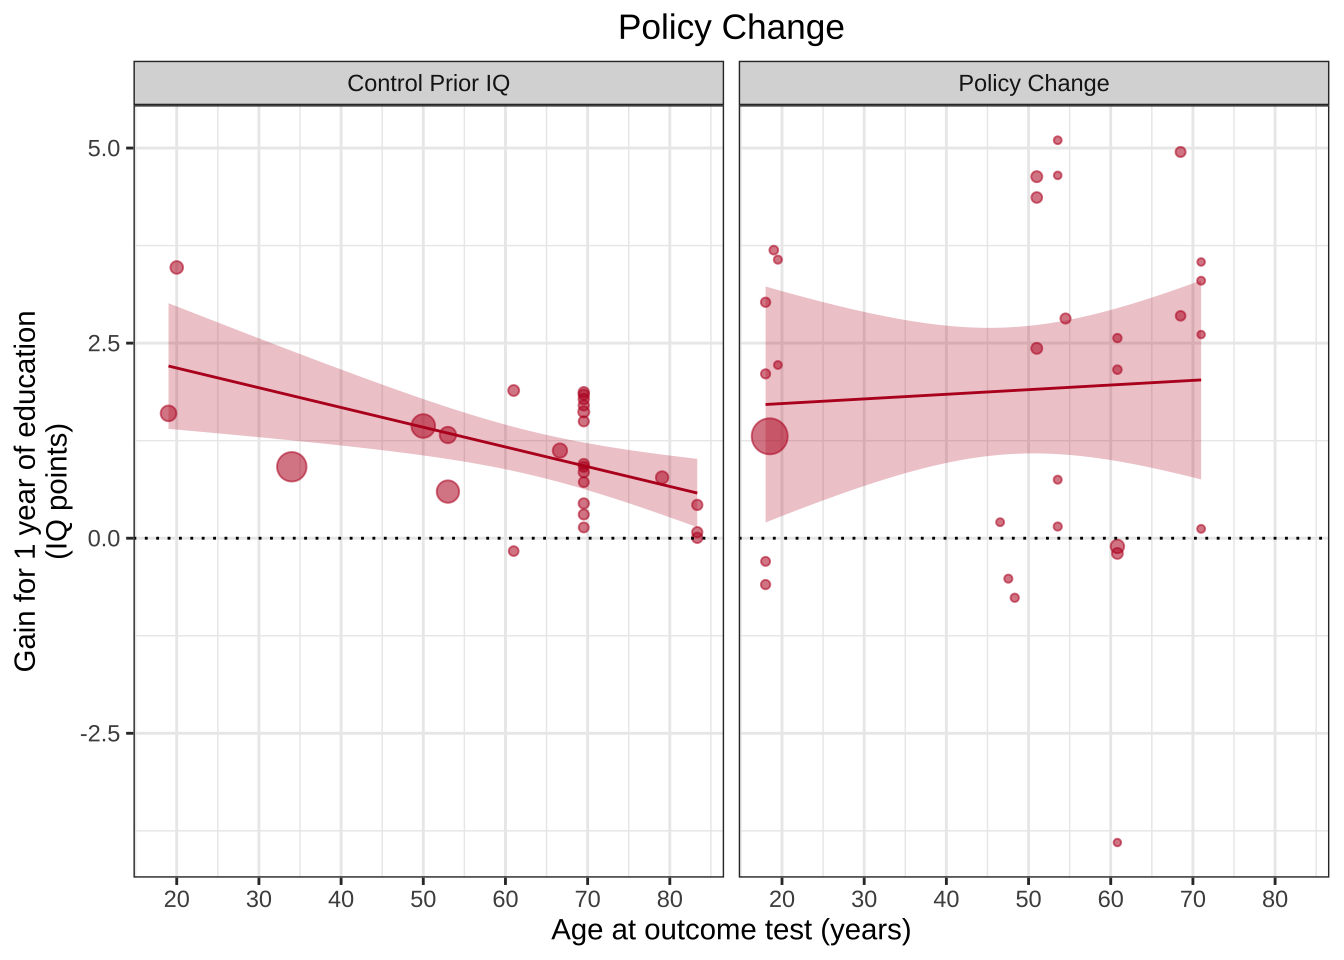
\includegraphics{210-desc_stats_files/figure-pdf/unnamed-chunk-32-1.pdf}

Применим разные функции, которые мы выучили:

\begin{Shaded}
\begin{Highlighting}[]
\FunctionTok{mean}\NormalTok{(xxx}\SpecialCharTok{$}\NormalTok{x)}
\end{Highlighting}
\end{Shaded}

\begin{verbatim}
[1] 54.26327
\end{verbatim}

\begin{Shaded}
\begin{Highlighting}[]
\FunctionTok{mean}\NormalTok{(xxx}\SpecialCharTok{$}\NormalTok{y)}
\end{Highlighting}
\end{Shaded}

\begin{verbatim}
[1] 47.83225
\end{verbatim}

\begin{Shaded}
\begin{Highlighting}[]
\FunctionTok{median}\NormalTok{(xxx}\SpecialCharTok{$}\NormalTok{x)}
\end{Highlighting}
\end{Shaded}

\begin{verbatim}
[1] 53.3333
\end{verbatim}

\begin{Shaded}
\begin{Highlighting}[]
\FunctionTok{median}\NormalTok{(xxx}\SpecialCharTok{$}\NormalTok{y)}
\end{Highlighting}
\end{Shaded}

\begin{verbatim}
[1] 46.0256
\end{verbatim}

Средние и медианы примерно одинаковые, при этом по \emph{х} они около
53-54, а по \emph{у} - примерно 46-47. Попытайтесь представить это. Идем
дальше:

\begin{Shaded}
\begin{Highlighting}[]
\FunctionTok{sd}\NormalTok{(xxx}\SpecialCharTok{$}\NormalTok{x)}
\end{Highlighting}
\end{Shaded}

\begin{verbatim}
[1] 16.76514
\end{verbatim}

\begin{Shaded}
\begin{Highlighting}[]
\FunctionTok{sd}\NormalTok{(xxx}\SpecialCharTok{$}\NormalTok{y)}
\end{Highlighting}
\end{Shaded}

\begin{verbatim}
[1] 26.9354
\end{verbatim}

Похоже, разброс по \emph{у} несколько больше, верно?

\begin{Shaded}
\begin{Highlighting}[]
\FunctionTok{skew}\NormalTok{(xxx}\SpecialCharTok{$}\NormalTok{x)}
\end{Highlighting}
\end{Shaded}

\begin{verbatim}
[1] 0.2807568
\end{verbatim}

\begin{Shaded}
\begin{Highlighting}[]
\FunctionTok{skew}\NormalTok{(xxx}\SpecialCharTok{$}\NormalTok{y)}
\end{Highlighting}
\end{Shaded}

\begin{verbatim}
[1] 0.2472603
\end{verbatim}

\begin{Shaded}
\begin{Highlighting}[]
\FunctionTok{kurtosi}\NormalTok{(xxx}\SpecialCharTok{$}\NormalTok{x)}
\end{Highlighting}
\end{Shaded}

\begin{verbatim}
[1] -0.2854912
\end{verbatim}

\begin{Shaded}
\begin{Highlighting}[]
\FunctionTok{kurtosi}\NormalTok{(xxx}\SpecialCharTok{$}\NormalTok{y)}
\end{Highlighting}
\end{Shaded}

\begin{verbatim}
[1] -1.063552
\end{verbatim}

Похоже, оба распределения немного право-ассиметричны и довольно
``плоские''.

Давайте еще посчитаем \textbf{коэффициент корреляции \emph{(correlation
coefficient)}}\emph{.} Мы про него будем говорить позже гораздо
подробнее (Глава~\ref{sec-cor}). Пока что нам нужно знать, что
\textbf{коэффициент корреляции} говорит о линейной связи двух
переменных. Если коэффициент корреляции \emph{положительный} (максимум
равен \texttt{1}), то чем \emph{больше} х, тем \emph{больше} у. Если
\emph{отрицательный} (минимум равен \texttt{-1}), то чем \emph{больше}
х, тем \emph{меньше} у. Если же коэффициент корреляции равен нулю, то
такая линейная зависимость отсутствует.

\begin{Shaded}
\begin{Highlighting}[]
\FunctionTok{cor}\NormalTok{(xxx}\SpecialCharTok{$}\NormalTok{x, xxx}\SpecialCharTok{$}\NormalTok{y)}
\end{Highlighting}
\end{Shaded}

\begin{verbatim}
[1] -0.06447185
\end{verbatim}

Коэффициент корреляции очень близка к нулю (делайте выводы и
представляйте).

Давайте напоследок воспользуемся функцией \texttt{describe()} из
\texttt{psych}:

\begin{Shaded}
\begin{Highlighting}[]
\NormalTok{psych}\SpecialCharTok{::}\FunctionTok{describe}\NormalTok{(xxx)}
\end{Highlighting}
\end{Shaded}

\begin{verbatim}
  vars   n  mean    sd median trimmed   mad   min   max range skew kurtosis
x    1 142 54.26 16.77  53.33   53.69 15.97 22.31 98.21 75.90 0.28    -0.29
y    2 142 47.83 26.94  46.03   46.90 30.79  2.95 99.49 96.54 0.25    -1.06
    se
x 1.41
y 2.26
\end{verbatim}

\begin{Shaded}
\begin{Highlighting}[]
\NormalTok{skimr}\SpecialCharTok{::}\FunctionTok{skim}\NormalTok{(xxx)}
\end{Highlighting}
\end{Shaded}

\begin{longtable}[]{@{}ll@{}}
\caption{Data summary}\tabularnewline
\toprule()
\endhead
Name & xxx \\
Number of rows & 142 \\
Number of columns & 2 \\
\_\_\_\_\_\_\_\_\_\_\_\_\_\_\_\_\_\_\_\_\_\_\_ & \\
Column type frequency: & \\
numeric & 2 \\
\_\_\_\_\_\_\_\_\_\_\_\_\_\_\_\_\_\_\_\_\_\_\_\_ & \\
Group variables & None \\
\bottomrule()
\end{longtable}

\textbf{Variable type: numeric}

\begin{longtable}[]{@{}
  >{\raggedright\arraybackslash}p{(\columnwidth - 20\tabcolsep) * \real{0.1628}}
  >{\raggedleft\arraybackslash}p{(\columnwidth - 20\tabcolsep) * \real{0.1163}}
  >{\raggedleft\arraybackslash}p{(\columnwidth - 20\tabcolsep) * \real{0.1628}}
  >{\raggedleft\arraybackslash}p{(\columnwidth - 20\tabcolsep) * \real{0.0698}}
  >{\raggedleft\arraybackslash}p{(\columnwidth - 20\tabcolsep) * \real{0.0698}}
  >{\raggedleft\arraybackslash}p{(\columnwidth - 20\tabcolsep) * \real{0.0698}}
  >{\raggedleft\arraybackslash}p{(\columnwidth - 20\tabcolsep) * \real{0.0698}}
  >{\raggedleft\arraybackslash}p{(\columnwidth - 20\tabcolsep) * \real{0.0698}}
  >{\raggedleft\arraybackslash}p{(\columnwidth - 20\tabcolsep) * \real{0.0698}}
  >{\raggedleft\arraybackslash}p{(\columnwidth - 20\tabcolsep) * \real{0.0698}}
  >{\raggedright\arraybackslash}p{(\columnwidth - 20\tabcolsep) * \real{0.0698}}@{}}
\toprule()
\begin{minipage}[b]{\linewidth}\raggedright
skim\_variable
\end{minipage} & \begin{minipage}[b]{\linewidth}\raggedleft
n\_missing
\end{minipage} & \begin{minipage}[b]{\linewidth}\raggedleft
complete\_rate
\end{minipage} & \begin{minipage}[b]{\linewidth}\raggedleft
mean
\end{minipage} & \begin{minipage}[b]{\linewidth}\raggedleft
sd
\end{minipage} & \begin{minipage}[b]{\linewidth}\raggedleft
p0
\end{minipage} & \begin{minipage}[b]{\linewidth}\raggedleft
p25
\end{minipage} & \begin{minipage}[b]{\linewidth}\raggedleft
p50
\end{minipage} & \begin{minipage}[b]{\linewidth}\raggedleft
p75
\end{minipage} & \begin{minipage}[b]{\linewidth}\raggedleft
p100
\end{minipage} & \begin{minipage}[b]{\linewidth}\raggedright
hist
\end{minipage} \\
\midrule()
\endhead
x & 0 & 1 & 54.26 & 16.77 & 22.31 & 44.10 & 53.33 & 64.74 & 98.21 &
▅▇▇▅▂ \\
y & 0 & 1 & 47.83 & 26.94 & 2.95 & 25.29 & 46.03 & 68.53 & 99.49 &
▇▇▇▅▆ \\
\bottomrule()
\end{longtable}

Готовы узнать, как выглядят эти данные на самом деле?!

Жмите сюда если готовы!

\begin{verbatim}
Warning in grid.Call(C_textBounds, as.graphicsAnnot(x$label), x$x, x$y, :
conversion failure on 'Это Датазавр!' in 'mbcsToSbcs': dot substituted for <d0>
\end{verbatim}

\begin{verbatim}
Warning in grid.Call(C_textBounds, as.graphicsAnnot(x$label), x$x, x$y, :
conversion failure on 'Это Датазавр!' in 'mbcsToSbcs': dot substituted for <ad>
\end{verbatim}

\begin{verbatim}
Warning in grid.Call(C_textBounds, as.graphicsAnnot(x$label), x$x, x$y, :
conversion failure on 'Это Датазавр!' in 'mbcsToSbcs': dot substituted for <d1>
\end{verbatim}

\begin{verbatim}
Warning in grid.Call(C_textBounds, as.graphicsAnnot(x$label), x$x, x$y, :
conversion failure on 'Это Датазавр!' in 'mbcsToSbcs': dot substituted for <82>
\end{verbatim}

\begin{verbatim}
Warning in grid.Call(C_textBounds, as.graphicsAnnot(x$label), x$x, x$y, :
conversion failure on 'Это Датазавр!' in 'mbcsToSbcs': dot substituted for <d0>
\end{verbatim}

\begin{verbatim}
Warning in grid.Call(C_textBounds, as.graphicsAnnot(x$label), x$x, x$y, :
conversion failure on 'Это Датазавр!' in 'mbcsToSbcs': dot substituted for <be>
\end{verbatim}

\begin{verbatim}
Warning in grid.Call(C_textBounds, as.graphicsAnnot(x$label), x$x, x$y, :
conversion failure on 'Это Датазавр!' in 'mbcsToSbcs': dot substituted for <d0>
\end{verbatim}

\begin{verbatim}
Warning in grid.Call(C_textBounds, as.graphicsAnnot(x$label), x$x, x$y, :
conversion failure on 'Это Датазавр!' in 'mbcsToSbcs': dot substituted for <94>
\end{verbatim}

\begin{verbatim}
Warning in grid.Call(C_textBounds, as.graphicsAnnot(x$label), x$x, x$y, :
conversion failure on 'Это Датазавр!' in 'mbcsToSbcs': dot substituted for <d0>
\end{verbatim}

\begin{verbatim}
Warning in grid.Call(C_textBounds, as.graphicsAnnot(x$label), x$x, x$y, :
conversion failure on 'Это Датазавр!' in 'mbcsToSbcs': dot substituted for <b0>
\end{verbatim}

\begin{verbatim}
Warning in grid.Call(C_textBounds, as.graphicsAnnot(x$label), x$x, x$y, :
conversion failure on 'Это Датазавр!' in 'mbcsToSbcs': dot substituted for <d1>
\end{verbatim}

\begin{verbatim}
Warning in grid.Call(C_textBounds, as.graphicsAnnot(x$label), x$x, x$y, :
conversion failure on 'Это Датазавр!' in 'mbcsToSbcs': dot substituted for <82>
\end{verbatim}

\begin{verbatim}
Warning in grid.Call(C_textBounds, as.graphicsAnnot(x$label), x$x, x$y, :
conversion failure on 'Это Датазавр!' in 'mbcsToSbcs': dot substituted for <d0>
\end{verbatim}

\begin{verbatim}
Warning in grid.Call(C_textBounds, as.graphicsAnnot(x$label), x$x, x$y, :
conversion failure on 'Это Датазавр!' in 'mbcsToSbcs': dot substituted for <b0>
\end{verbatim}

\begin{verbatim}
Warning in grid.Call(C_textBounds, as.graphicsAnnot(x$label), x$x, x$y, :
conversion failure on 'Это Датазавр!' in 'mbcsToSbcs': dot substituted for <d0>
\end{verbatim}

\begin{verbatim}
Warning in grid.Call(C_textBounds, as.graphicsAnnot(x$label), x$x, x$y, :
conversion failure on 'Это Датазавр!' in 'mbcsToSbcs': dot substituted for <b7>
\end{verbatim}

\begin{verbatim}
Warning in grid.Call(C_textBounds, as.graphicsAnnot(x$label), x$x, x$y, :
conversion failure on 'Это Датазавр!' in 'mbcsToSbcs': dot substituted for <d0>
\end{verbatim}

\begin{verbatim}
Warning in grid.Call(C_textBounds, as.graphicsAnnot(x$label), x$x, x$y, :
conversion failure on 'Это Датазавр!' in 'mbcsToSbcs': dot substituted for <b0>
\end{verbatim}

\begin{verbatim}
Warning in grid.Call(C_textBounds, as.graphicsAnnot(x$label), x$x, x$y, :
conversion failure on 'Это Датазавр!' in 'mbcsToSbcs': dot substituted for <d0>
\end{verbatim}

\begin{verbatim}
Warning in grid.Call(C_textBounds, as.graphicsAnnot(x$label), x$x, x$y, :
conversion failure on 'Это Датазавр!' in 'mbcsToSbcs': dot substituted for <b2>
\end{verbatim}

\begin{verbatim}
Warning in grid.Call(C_textBounds, as.graphicsAnnot(x$label), x$x, x$y, :
conversion failure on 'Это Датазавр!' in 'mbcsToSbcs': dot substituted for <d1>
\end{verbatim}

\begin{verbatim}
Warning in grid.Call(C_textBounds, as.graphicsAnnot(x$label), x$x, x$y, :
conversion failure on 'Это Датазавр!' in 'mbcsToSbcs': dot substituted for <80>
\end{verbatim}

\begin{verbatim}
Warning in grid.Call(C_textBounds, as.graphicsAnnot(x$label), x$x, x$y, :
conversion failure on 'Это Датазавр!' in 'mbcsToSbcs': dot substituted for <d0>
\end{verbatim}

\begin{verbatim}
Warning in grid.Call(C_textBounds, as.graphicsAnnot(x$label), x$x, x$y, :
conversion failure on 'Это Датазавр!' in 'mbcsToSbcs': dot substituted for <ad>
\end{verbatim}

\begin{verbatim}
Warning in grid.Call(C_textBounds, as.graphicsAnnot(x$label), x$x, x$y, :
conversion failure on 'Это Датазавр!' in 'mbcsToSbcs': dot substituted for <d1>
\end{verbatim}

\begin{verbatim}
Warning in grid.Call(C_textBounds, as.graphicsAnnot(x$label), x$x, x$y, :
conversion failure on 'Это Датазавр!' in 'mbcsToSbcs': dot substituted for <82>
\end{verbatim}

\begin{verbatim}
Warning in grid.Call(C_textBounds, as.graphicsAnnot(x$label), x$x, x$y, :
conversion failure on 'Это Датазавр!' in 'mbcsToSbcs': dot substituted for <d0>
\end{verbatim}

\begin{verbatim}
Warning in grid.Call(C_textBounds, as.graphicsAnnot(x$label), x$x, x$y, :
conversion failure on 'Это Датазавр!' in 'mbcsToSbcs': dot substituted for <be>
\end{verbatim}

\begin{verbatim}
Warning in grid.Call(C_textBounds, as.graphicsAnnot(x$label), x$x, x$y, :
conversion failure on 'Это Датазавр!' in 'mbcsToSbcs': dot substituted for <d0>
\end{verbatim}

\begin{verbatim}
Warning in grid.Call(C_textBounds, as.graphicsAnnot(x$label), x$x, x$y, :
conversion failure on 'Это Датазавр!' in 'mbcsToSbcs': dot substituted for <94>
\end{verbatim}

\begin{verbatim}
Warning in grid.Call(C_textBounds, as.graphicsAnnot(x$label), x$x, x$y, :
conversion failure on 'Это Датазавр!' in 'mbcsToSbcs': dot substituted for <d0>
\end{verbatim}

\begin{verbatim}
Warning in grid.Call(C_textBounds, as.graphicsAnnot(x$label), x$x, x$y, :
conversion failure on 'Это Датазавр!' in 'mbcsToSbcs': dot substituted for <b0>
\end{verbatim}

\begin{verbatim}
Warning in grid.Call(C_textBounds, as.graphicsAnnot(x$label), x$x, x$y, :
conversion failure on 'Это Датазавр!' in 'mbcsToSbcs': dot substituted for <d1>
\end{verbatim}

\begin{verbatim}
Warning in grid.Call(C_textBounds, as.graphicsAnnot(x$label), x$x, x$y, :
conversion failure on 'Это Датазавр!' in 'mbcsToSbcs': dot substituted for <82>
\end{verbatim}

\begin{verbatim}
Warning in grid.Call(C_textBounds, as.graphicsAnnot(x$label), x$x, x$y, :
conversion failure on 'Это Датазавр!' in 'mbcsToSbcs': dot substituted for <d0>
\end{verbatim}

\begin{verbatim}
Warning in grid.Call(C_textBounds, as.graphicsAnnot(x$label), x$x, x$y, :
conversion failure on 'Это Датазавр!' in 'mbcsToSbcs': dot substituted for <b0>
\end{verbatim}

\begin{verbatim}
Warning in grid.Call(C_textBounds, as.graphicsAnnot(x$label), x$x, x$y, :
conversion failure on 'Это Датазавр!' in 'mbcsToSbcs': dot substituted for <d0>
\end{verbatim}

\begin{verbatim}
Warning in grid.Call(C_textBounds, as.graphicsAnnot(x$label), x$x, x$y, :
conversion failure on 'Это Датазавр!' in 'mbcsToSbcs': dot substituted for <b7>
\end{verbatim}

\begin{verbatim}
Warning in grid.Call(C_textBounds, as.graphicsAnnot(x$label), x$x, x$y, :
conversion failure on 'Это Датазавр!' in 'mbcsToSbcs': dot substituted for <d0>
\end{verbatim}

\begin{verbatim}
Warning in grid.Call(C_textBounds, as.graphicsAnnot(x$label), x$x, x$y, :
conversion failure on 'Это Датазавр!' in 'mbcsToSbcs': dot substituted for <b0>
\end{verbatim}

\begin{verbatim}
Warning in grid.Call(C_textBounds, as.graphicsAnnot(x$label), x$x, x$y, :
conversion failure on 'Это Датазавр!' in 'mbcsToSbcs': dot substituted for <d0>
\end{verbatim}

\begin{verbatim}
Warning in grid.Call(C_textBounds, as.graphicsAnnot(x$label), x$x, x$y, :
conversion failure on 'Это Датазавр!' in 'mbcsToSbcs': dot substituted for <b2>
\end{verbatim}

\begin{verbatim}
Warning in grid.Call(C_textBounds, as.graphicsAnnot(x$label), x$x, x$y, :
conversion failure on 'Это Датазавр!' in 'mbcsToSbcs': dot substituted for <d1>
\end{verbatim}

\begin{verbatim}
Warning in grid.Call(C_textBounds, as.graphicsAnnot(x$label), x$x, x$y, :
conversion failure on 'Это Датазавр!' in 'mbcsToSbcs': dot substituted for <80>
\end{verbatim}

\begin{verbatim}
Warning in grid.Call(C_textBounds, as.graphicsAnnot(x$label), x$x, x$y, :
conversion failure on 'Это Датазавр!' in 'mbcsToSbcs': dot substituted for <d0>
\end{verbatim}

\begin{verbatim}
Warning in grid.Call(C_textBounds, as.graphicsAnnot(x$label), x$x, x$y, :
conversion failure on 'Это Датазавр!' in 'mbcsToSbcs': dot substituted for <ad>
\end{verbatim}

\begin{verbatim}
Warning in grid.Call(C_textBounds, as.graphicsAnnot(x$label), x$x, x$y, :
conversion failure on 'Это Датазавр!' in 'mbcsToSbcs': dot substituted for <d1>
\end{verbatim}

\begin{verbatim}
Warning in grid.Call(C_textBounds, as.graphicsAnnot(x$label), x$x, x$y, :
conversion failure on 'Это Датазавр!' in 'mbcsToSbcs': dot substituted for <82>
\end{verbatim}

\begin{verbatim}
Warning in grid.Call(C_textBounds, as.graphicsAnnot(x$label), x$x, x$y, :
conversion failure on 'Это Датазавр!' in 'mbcsToSbcs': dot substituted for <d0>
\end{verbatim}

\begin{verbatim}
Warning in grid.Call(C_textBounds, as.graphicsAnnot(x$label), x$x, x$y, :
conversion failure on 'Это Датазавр!' in 'mbcsToSbcs': dot substituted for <be>
\end{verbatim}

\begin{verbatim}
Warning in grid.Call(C_textBounds, as.graphicsAnnot(x$label), x$x, x$y, :
conversion failure on 'Это Датазавр!' in 'mbcsToSbcs': dot substituted for <d0>
\end{verbatim}

\begin{verbatim}
Warning in grid.Call(C_textBounds, as.graphicsAnnot(x$label), x$x, x$y, :
conversion failure on 'Это Датазавр!' in 'mbcsToSbcs': dot substituted for <94>
\end{verbatim}

\begin{verbatim}
Warning in grid.Call(C_textBounds, as.graphicsAnnot(x$label), x$x, x$y, :
conversion failure on 'Это Датазавр!' in 'mbcsToSbcs': dot substituted for <d0>
\end{verbatim}

\begin{verbatim}
Warning in grid.Call(C_textBounds, as.graphicsAnnot(x$label), x$x, x$y, :
conversion failure on 'Это Датазавр!' in 'mbcsToSbcs': dot substituted for <b0>
\end{verbatim}

\begin{verbatim}
Warning in grid.Call(C_textBounds, as.graphicsAnnot(x$label), x$x, x$y, :
conversion failure on 'Это Датазавр!' in 'mbcsToSbcs': dot substituted for <d1>
\end{verbatim}

\begin{verbatim}
Warning in grid.Call(C_textBounds, as.graphicsAnnot(x$label), x$x, x$y, :
conversion failure on 'Это Датазавр!' in 'mbcsToSbcs': dot substituted for <82>
\end{verbatim}

\begin{verbatim}
Warning in grid.Call(C_textBounds, as.graphicsAnnot(x$label), x$x, x$y, :
conversion failure on 'Это Датазавр!' in 'mbcsToSbcs': dot substituted for <d0>
\end{verbatim}

\begin{verbatim}
Warning in grid.Call(C_textBounds, as.graphicsAnnot(x$label), x$x, x$y, :
conversion failure on 'Это Датазавр!' in 'mbcsToSbcs': dot substituted for <b0>
\end{verbatim}

\begin{verbatim}
Warning in grid.Call(C_textBounds, as.graphicsAnnot(x$label), x$x, x$y, :
conversion failure on 'Это Датазавр!' in 'mbcsToSbcs': dot substituted for <d0>
\end{verbatim}

\begin{verbatim}
Warning in grid.Call(C_textBounds, as.graphicsAnnot(x$label), x$x, x$y, :
conversion failure on 'Это Датазавр!' in 'mbcsToSbcs': dot substituted for <b7>
\end{verbatim}

\begin{verbatim}
Warning in grid.Call(C_textBounds, as.graphicsAnnot(x$label), x$x, x$y, :
conversion failure on 'Это Датазавр!' in 'mbcsToSbcs': dot substituted for <d0>
\end{verbatim}

\begin{verbatim}
Warning in grid.Call(C_textBounds, as.graphicsAnnot(x$label), x$x, x$y, :
conversion failure on 'Это Датазавр!' in 'mbcsToSbcs': dot substituted for <b0>
\end{verbatim}

\begin{verbatim}
Warning in grid.Call(C_textBounds, as.graphicsAnnot(x$label), x$x, x$y, :
conversion failure on 'Это Датазавр!' in 'mbcsToSbcs': dot substituted for <d0>
\end{verbatim}

\begin{verbatim}
Warning in grid.Call(C_textBounds, as.graphicsAnnot(x$label), x$x, x$y, :
conversion failure on 'Это Датазавр!' in 'mbcsToSbcs': dot substituted for <b2>
\end{verbatim}

\begin{verbatim}
Warning in grid.Call(C_textBounds, as.graphicsAnnot(x$label), x$x, x$y, :
conversion failure on 'Это Датазавр!' in 'mbcsToSbcs': dot substituted for <d1>
\end{verbatim}

\begin{verbatim}
Warning in grid.Call(C_textBounds, as.graphicsAnnot(x$label), x$x, x$y, :
conversion failure on 'Это Датазавр!' in 'mbcsToSbcs': dot substituted for <80>
\end{verbatim}

\begin{verbatim}
Warning in grid.Call(C_textBounds, as.graphicsAnnot(x$label), x$x, x$y, :
conversion failure on 'Это Датазавр!' in 'mbcsToSbcs': dot substituted for <d0>
\end{verbatim}

\begin{verbatim}
Warning in grid.Call(C_textBounds, as.graphicsAnnot(x$label), x$x, x$y, :
conversion failure on 'Это Датазавр!' in 'mbcsToSbcs': dot substituted for <ad>
\end{verbatim}

\begin{verbatim}
Warning in grid.Call(C_textBounds, as.graphicsAnnot(x$label), x$x, x$y, :
conversion failure on 'Это Датазавр!' in 'mbcsToSbcs': dot substituted for <d1>
\end{verbatim}

\begin{verbatim}
Warning in grid.Call(C_textBounds, as.graphicsAnnot(x$label), x$x, x$y, :
conversion failure on 'Это Датазавр!' in 'mbcsToSbcs': dot substituted for <82>
\end{verbatim}

\begin{verbatim}
Warning in grid.Call(C_textBounds, as.graphicsAnnot(x$label), x$x, x$y, :
conversion failure on 'Это Датазавр!' in 'mbcsToSbcs': dot substituted for <d0>
\end{verbatim}

\begin{verbatim}
Warning in grid.Call(C_textBounds, as.graphicsAnnot(x$label), x$x, x$y, :
conversion failure on 'Это Датазавр!' in 'mbcsToSbcs': dot substituted for <be>
\end{verbatim}

\begin{verbatim}
Warning in grid.Call(C_textBounds, as.graphicsAnnot(x$label), x$x, x$y, :
conversion failure on 'Это Датазавр!' in 'mbcsToSbcs': dot substituted for <d0>
\end{verbatim}

\begin{verbatim}
Warning in grid.Call(C_textBounds, as.graphicsAnnot(x$label), x$x, x$y, :
conversion failure on 'Это Датазавр!' in 'mbcsToSbcs': dot substituted for <94>
\end{verbatim}

\begin{verbatim}
Warning in grid.Call(C_textBounds, as.graphicsAnnot(x$label), x$x, x$y, :
conversion failure on 'Это Датазавр!' in 'mbcsToSbcs': dot substituted for <d0>
\end{verbatim}

\begin{verbatim}
Warning in grid.Call(C_textBounds, as.graphicsAnnot(x$label), x$x, x$y, :
conversion failure on 'Это Датазавр!' in 'mbcsToSbcs': dot substituted for <b0>
\end{verbatim}

\begin{verbatim}
Warning in grid.Call(C_textBounds, as.graphicsAnnot(x$label), x$x, x$y, :
conversion failure on 'Это Датазавр!' in 'mbcsToSbcs': dot substituted for <d1>
\end{verbatim}

\begin{verbatim}
Warning in grid.Call(C_textBounds, as.graphicsAnnot(x$label), x$x, x$y, :
conversion failure on 'Это Датазавр!' in 'mbcsToSbcs': dot substituted for <82>
\end{verbatim}

\begin{verbatim}
Warning in grid.Call(C_textBounds, as.graphicsAnnot(x$label), x$x, x$y, :
conversion failure on 'Это Датазавр!' in 'mbcsToSbcs': dot substituted for <d0>
\end{verbatim}

\begin{verbatim}
Warning in grid.Call(C_textBounds, as.graphicsAnnot(x$label), x$x, x$y, :
conversion failure on 'Это Датазавр!' in 'mbcsToSbcs': dot substituted for <b0>
\end{verbatim}

\begin{verbatim}
Warning in grid.Call(C_textBounds, as.graphicsAnnot(x$label), x$x, x$y, :
conversion failure on 'Это Датазавр!' in 'mbcsToSbcs': dot substituted for <d0>
\end{verbatim}

\begin{verbatim}
Warning in grid.Call(C_textBounds, as.graphicsAnnot(x$label), x$x, x$y, :
conversion failure on 'Это Датазавр!' in 'mbcsToSbcs': dot substituted for <b7>
\end{verbatim}

\begin{verbatim}
Warning in grid.Call(C_textBounds, as.graphicsAnnot(x$label), x$x, x$y, :
conversion failure on 'Это Датазавр!' in 'mbcsToSbcs': dot substituted for <d0>
\end{verbatim}

\begin{verbatim}
Warning in grid.Call(C_textBounds, as.graphicsAnnot(x$label), x$x, x$y, :
conversion failure on 'Это Датазавр!' in 'mbcsToSbcs': dot substituted for <b0>
\end{verbatim}

\begin{verbatim}
Warning in grid.Call(C_textBounds, as.graphicsAnnot(x$label), x$x, x$y, :
conversion failure on 'Это Датазавр!' in 'mbcsToSbcs': dot substituted for <d0>
\end{verbatim}

\begin{verbatim}
Warning in grid.Call(C_textBounds, as.graphicsAnnot(x$label), x$x, x$y, :
conversion failure on 'Это Датазавр!' in 'mbcsToSbcs': dot substituted for <b2>
\end{verbatim}

\begin{verbatim}
Warning in grid.Call(C_textBounds, as.graphicsAnnot(x$label), x$x, x$y, :
conversion failure on 'Это Датазавр!' in 'mbcsToSbcs': dot substituted for <d1>
\end{verbatim}

\begin{verbatim}
Warning in grid.Call(C_textBounds, as.graphicsAnnot(x$label), x$x, x$y, :
conversion failure on 'Это Датазавр!' in 'mbcsToSbcs': dot substituted for <80>
\end{verbatim}

\begin{verbatim}
Warning in grid.Call(C_textBounds, as.graphicsAnnot(x$label), x$x, x$y, :
conversion failure on 'Это Датазавр!' in 'mbcsToSbcs': dot substituted for <d0>
\end{verbatim}

\begin{verbatim}
Warning in grid.Call(C_textBounds, as.graphicsAnnot(x$label), x$x, x$y, :
conversion failure on 'Это Датазавр!' in 'mbcsToSbcs': dot substituted for <ad>
\end{verbatim}

\begin{verbatim}
Warning in grid.Call(C_textBounds, as.graphicsAnnot(x$label), x$x, x$y, :
conversion failure on 'Это Датазавр!' in 'mbcsToSbcs': dot substituted for <d1>
\end{verbatim}

\begin{verbatim}
Warning in grid.Call(C_textBounds, as.graphicsAnnot(x$label), x$x, x$y, :
conversion failure on 'Это Датазавр!' in 'mbcsToSbcs': dot substituted for <82>
\end{verbatim}

\begin{verbatim}
Warning in grid.Call(C_textBounds, as.graphicsAnnot(x$label), x$x, x$y, :
conversion failure on 'Это Датазавр!' in 'mbcsToSbcs': dot substituted for <d0>
\end{verbatim}

\begin{verbatim}
Warning in grid.Call(C_textBounds, as.graphicsAnnot(x$label), x$x, x$y, :
conversion failure on 'Это Датазавр!' in 'mbcsToSbcs': dot substituted for <be>
\end{verbatim}

\begin{verbatim}
Warning in grid.Call(C_textBounds, as.graphicsAnnot(x$label), x$x, x$y, :
conversion failure on 'Это Датазавр!' in 'mbcsToSbcs': dot substituted for <d0>
\end{verbatim}

\begin{verbatim}
Warning in grid.Call(C_textBounds, as.graphicsAnnot(x$label), x$x, x$y, :
conversion failure on 'Это Датазавр!' in 'mbcsToSbcs': dot substituted for <94>
\end{verbatim}

\begin{verbatim}
Warning in grid.Call(C_textBounds, as.graphicsAnnot(x$label), x$x, x$y, :
conversion failure on 'Это Датазавр!' in 'mbcsToSbcs': dot substituted for <d0>
\end{verbatim}

\begin{verbatim}
Warning in grid.Call(C_textBounds, as.graphicsAnnot(x$label), x$x, x$y, :
conversion failure on 'Это Датазавр!' in 'mbcsToSbcs': dot substituted for <b0>
\end{verbatim}

\begin{verbatim}
Warning in grid.Call(C_textBounds, as.graphicsAnnot(x$label), x$x, x$y, :
conversion failure on 'Это Датазавр!' in 'mbcsToSbcs': dot substituted for <d1>
\end{verbatim}

\begin{verbatim}
Warning in grid.Call(C_textBounds, as.graphicsAnnot(x$label), x$x, x$y, :
conversion failure on 'Это Датазавр!' in 'mbcsToSbcs': dot substituted for <82>
\end{verbatim}

\begin{verbatim}
Warning in grid.Call(C_textBounds, as.graphicsAnnot(x$label), x$x, x$y, :
conversion failure on 'Это Датазавр!' in 'mbcsToSbcs': dot substituted for <d0>
\end{verbatim}

\begin{verbatim}
Warning in grid.Call(C_textBounds, as.graphicsAnnot(x$label), x$x, x$y, :
conversion failure on 'Это Датазавр!' in 'mbcsToSbcs': dot substituted for <b0>
\end{verbatim}

\begin{verbatim}
Warning in grid.Call(C_textBounds, as.graphicsAnnot(x$label), x$x, x$y, :
conversion failure on 'Это Датазавр!' in 'mbcsToSbcs': dot substituted for <d0>
\end{verbatim}

\begin{verbatim}
Warning in grid.Call(C_textBounds, as.graphicsAnnot(x$label), x$x, x$y, :
conversion failure on 'Это Датазавр!' in 'mbcsToSbcs': dot substituted for <b7>
\end{verbatim}

\begin{verbatim}
Warning in grid.Call(C_textBounds, as.graphicsAnnot(x$label), x$x, x$y, :
conversion failure on 'Это Датазавр!' in 'mbcsToSbcs': dot substituted for <d0>
\end{verbatim}

\begin{verbatim}
Warning in grid.Call(C_textBounds, as.graphicsAnnot(x$label), x$x, x$y, :
conversion failure on 'Это Датазавр!' in 'mbcsToSbcs': dot substituted for <b0>
\end{verbatim}

\begin{verbatim}
Warning in grid.Call(C_textBounds, as.graphicsAnnot(x$label), x$x, x$y, :
conversion failure on 'Это Датазавр!' in 'mbcsToSbcs': dot substituted for <d0>
\end{verbatim}

\begin{verbatim}
Warning in grid.Call(C_textBounds, as.graphicsAnnot(x$label), x$x, x$y, :
conversion failure on 'Это Датазавр!' in 'mbcsToSbcs': dot substituted for <b2>
\end{verbatim}

\begin{verbatim}
Warning in grid.Call(C_textBounds, as.graphicsAnnot(x$label), x$x, x$y, :
conversion failure on 'Это Датазавр!' in 'mbcsToSbcs': dot substituted for <d1>
\end{verbatim}

\begin{verbatim}
Warning in grid.Call(C_textBounds, as.graphicsAnnot(x$label), x$x, x$y, :
conversion failure on 'Это Датазавр!' in 'mbcsToSbcs': dot substituted for <80>
\end{verbatim}

\begin{verbatim}
Warning in grid.Call(C_textBounds, as.graphicsAnnot(x$label), x$x, x$y, :
conversion failure on 'Это Датазавр!' in 'mbcsToSbcs': dot substituted for <d0>
\end{verbatim}

\begin{verbatim}
Warning in grid.Call(C_textBounds, as.graphicsAnnot(x$label), x$x, x$y, :
conversion failure on 'Это Датазавр!' in 'mbcsToSbcs': dot substituted for <ad>
\end{verbatim}

\begin{verbatim}
Warning in grid.Call(C_textBounds, as.graphicsAnnot(x$label), x$x, x$y, :
conversion failure on 'Это Датазавр!' in 'mbcsToSbcs': dot substituted for <d1>
\end{verbatim}

\begin{verbatim}
Warning in grid.Call(C_textBounds, as.graphicsAnnot(x$label), x$x, x$y, :
conversion failure on 'Это Датазавр!' in 'mbcsToSbcs': dot substituted for <82>
\end{verbatim}

\begin{verbatim}
Warning in grid.Call(C_textBounds, as.graphicsAnnot(x$label), x$x, x$y, :
conversion failure on 'Это Датазавр!' in 'mbcsToSbcs': dot substituted for <d0>
\end{verbatim}

\begin{verbatim}
Warning in grid.Call(C_textBounds, as.graphicsAnnot(x$label), x$x, x$y, :
conversion failure on 'Это Датазавр!' in 'mbcsToSbcs': dot substituted for <be>
\end{verbatim}

\begin{verbatim}
Warning in grid.Call(C_textBounds, as.graphicsAnnot(x$label), x$x, x$y, :
conversion failure on 'Это Датазавр!' in 'mbcsToSbcs': dot substituted for <d0>
\end{verbatim}

\begin{verbatim}
Warning in grid.Call(C_textBounds, as.graphicsAnnot(x$label), x$x, x$y, :
conversion failure on 'Это Датазавр!' in 'mbcsToSbcs': dot substituted for <94>
\end{verbatim}

\begin{verbatim}
Warning in grid.Call(C_textBounds, as.graphicsAnnot(x$label), x$x, x$y, :
conversion failure on 'Это Датазавр!' in 'mbcsToSbcs': dot substituted for <d0>
\end{verbatim}

\begin{verbatim}
Warning in grid.Call(C_textBounds, as.graphicsAnnot(x$label), x$x, x$y, :
conversion failure on 'Это Датазавр!' in 'mbcsToSbcs': dot substituted for <b0>
\end{verbatim}

\begin{verbatim}
Warning in grid.Call(C_textBounds, as.graphicsAnnot(x$label), x$x, x$y, :
conversion failure on 'Это Датазавр!' in 'mbcsToSbcs': dot substituted for <d1>
\end{verbatim}

\begin{verbatim}
Warning in grid.Call(C_textBounds, as.graphicsAnnot(x$label), x$x, x$y, :
conversion failure on 'Это Датазавр!' in 'mbcsToSbcs': dot substituted for <82>
\end{verbatim}

\begin{verbatim}
Warning in grid.Call(C_textBounds, as.graphicsAnnot(x$label), x$x, x$y, :
conversion failure on 'Это Датазавр!' in 'mbcsToSbcs': dot substituted for <d0>
\end{verbatim}

\begin{verbatim}
Warning in grid.Call(C_textBounds, as.graphicsAnnot(x$label), x$x, x$y, :
conversion failure on 'Это Датазавр!' in 'mbcsToSbcs': dot substituted for <b0>
\end{verbatim}

\begin{verbatim}
Warning in grid.Call(C_textBounds, as.graphicsAnnot(x$label), x$x, x$y, :
conversion failure on 'Это Датазавр!' in 'mbcsToSbcs': dot substituted for <d0>
\end{verbatim}

\begin{verbatim}
Warning in grid.Call(C_textBounds, as.graphicsAnnot(x$label), x$x, x$y, :
conversion failure on 'Это Датазавр!' in 'mbcsToSbcs': dot substituted for <b7>
\end{verbatim}

\begin{verbatim}
Warning in grid.Call(C_textBounds, as.graphicsAnnot(x$label), x$x, x$y, :
conversion failure on 'Это Датазавр!' in 'mbcsToSbcs': dot substituted for <d0>
\end{verbatim}

\begin{verbatim}
Warning in grid.Call(C_textBounds, as.graphicsAnnot(x$label), x$x, x$y, :
conversion failure on 'Это Датазавр!' in 'mbcsToSbcs': dot substituted for <b0>
\end{verbatim}

\begin{verbatim}
Warning in grid.Call(C_textBounds, as.graphicsAnnot(x$label), x$x, x$y, :
conversion failure on 'Это Датазавр!' in 'mbcsToSbcs': dot substituted for <d0>
\end{verbatim}

\begin{verbatim}
Warning in grid.Call(C_textBounds, as.graphicsAnnot(x$label), x$x, x$y, :
conversion failure on 'Это Датазавр!' in 'mbcsToSbcs': dot substituted for <b2>
\end{verbatim}

\begin{verbatim}
Warning in grid.Call(C_textBounds, as.graphicsAnnot(x$label), x$x, x$y, :
conversion failure on 'Это Датазавр!' in 'mbcsToSbcs': dot substituted for <d1>
\end{verbatim}

\begin{verbatim}
Warning in grid.Call(C_textBounds, as.graphicsAnnot(x$label), x$x, x$y, :
conversion failure on 'Это Датазавр!' in 'mbcsToSbcs': dot substituted for <80>
\end{verbatim}

\begin{verbatim}
Warning in grid.Call(C_textBounds, as.graphicsAnnot(x$label), x$x, x$y, :
conversion failure on 'Это Датазавр!' in 'mbcsToSbcs': dot substituted for <d0>
\end{verbatim}

\begin{verbatim}
Warning in grid.Call(C_textBounds, as.graphicsAnnot(x$label), x$x, x$y, :
conversion failure on 'Это Датазавр!' in 'mbcsToSbcs': dot substituted for <ad>
\end{verbatim}

\begin{verbatim}
Warning in grid.Call(C_textBounds, as.graphicsAnnot(x$label), x$x, x$y, :
conversion failure on 'Это Датазавр!' in 'mbcsToSbcs': dot substituted for <d1>
\end{verbatim}

\begin{verbatim}
Warning in grid.Call(C_textBounds, as.graphicsAnnot(x$label), x$x, x$y, :
conversion failure on 'Это Датазавр!' in 'mbcsToSbcs': dot substituted for <82>
\end{verbatim}

\begin{verbatim}
Warning in grid.Call(C_textBounds, as.graphicsAnnot(x$label), x$x, x$y, :
conversion failure on 'Это Датазавр!' in 'mbcsToSbcs': dot substituted for <d0>
\end{verbatim}

\begin{verbatim}
Warning in grid.Call(C_textBounds, as.graphicsAnnot(x$label), x$x, x$y, :
conversion failure on 'Это Датазавр!' in 'mbcsToSbcs': dot substituted for <be>
\end{verbatim}

\begin{verbatim}
Warning in grid.Call(C_textBounds, as.graphicsAnnot(x$label), x$x, x$y, :
conversion failure on 'Это Датазавр!' in 'mbcsToSbcs': dot substituted for <d0>
\end{verbatim}

\begin{verbatim}
Warning in grid.Call(C_textBounds, as.graphicsAnnot(x$label), x$x, x$y, :
conversion failure on 'Это Датазавр!' in 'mbcsToSbcs': dot substituted for <94>
\end{verbatim}

\begin{verbatim}
Warning in grid.Call(C_textBounds, as.graphicsAnnot(x$label), x$x, x$y, :
conversion failure on 'Это Датазавр!' in 'mbcsToSbcs': dot substituted for <d0>
\end{verbatim}

\begin{verbatim}
Warning in grid.Call(C_textBounds, as.graphicsAnnot(x$label), x$x, x$y, :
conversion failure on 'Это Датазавр!' in 'mbcsToSbcs': dot substituted for <b0>
\end{verbatim}

\begin{verbatim}
Warning in grid.Call(C_textBounds, as.graphicsAnnot(x$label), x$x, x$y, :
conversion failure on 'Это Датазавр!' in 'mbcsToSbcs': dot substituted for <d1>
\end{verbatim}

\begin{verbatim}
Warning in grid.Call(C_textBounds, as.graphicsAnnot(x$label), x$x, x$y, :
conversion failure on 'Это Датазавр!' in 'mbcsToSbcs': dot substituted for <82>
\end{verbatim}

\begin{verbatim}
Warning in grid.Call(C_textBounds, as.graphicsAnnot(x$label), x$x, x$y, :
conversion failure on 'Это Датазавр!' in 'mbcsToSbcs': dot substituted for <d0>
\end{verbatim}

\begin{verbatim}
Warning in grid.Call(C_textBounds, as.graphicsAnnot(x$label), x$x, x$y, :
conversion failure on 'Это Датазавр!' in 'mbcsToSbcs': dot substituted for <b0>
\end{verbatim}

\begin{verbatim}
Warning in grid.Call(C_textBounds, as.graphicsAnnot(x$label), x$x, x$y, :
conversion failure on 'Это Датазавр!' in 'mbcsToSbcs': dot substituted for <d0>
\end{verbatim}

\begin{verbatim}
Warning in grid.Call(C_textBounds, as.graphicsAnnot(x$label), x$x, x$y, :
conversion failure on 'Это Датазавр!' in 'mbcsToSbcs': dot substituted for <b7>
\end{verbatim}

\begin{verbatim}
Warning in grid.Call(C_textBounds, as.graphicsAnnot(x$label), x$x, x$y, :
conversion failure on 'Это Датазавр!' in 'mbcsToSbcs': dot substituted for <d0>
\end{verbatim}

\begin{verbatim}
Warning in grid.Call(C_textBounds, as.graphicsAnnot(x$label), x$x, x$y, :
conversion failure on 'Это Датазавр!' in 'mbcsToSbcs': dot substituted for <b0>
\end{verbatim}

\begin{verbatim}
Warning in grid.Call(C_textBounds, as.graphicsAnnot(x$label), x$x, x$y, :
conversion failure on 'Это Датазавр!' in 'mbcsToSbcs': dot substituted for <d0>
\end{verbatim}

\begin{verbatim}
Warning in grid.Call(C_textBounds, as.graphicsAnnot(x$label), x$x, x$y, :
conversion failure on 'Это Датазавр!' in 'mbcsToSbcs': dot substituted for <b2>
\end{verbatim}

\begin{verbatim}
Warning in grid.Call(C_textBounds, as.graphicsAnnot(x$label), x$x, x$y, :
conversion failure on 'Это Датазавр!' in 'mbcsToSbcs': dot substituted for <d1>
\end{verbatim}

\begin{verbatim}
Warning in grid.Call(C_textBounds, as.graphicsAnnot(x$label), x$x, x$y, :
conversion failure on 'Это Датазавр!' in 'mbcsToSbcs': dot substituted for <80>
\end{verbatim}

\begin{verbatim}
Warning in grid.Call.graphics(C_text, as.graphicsAnnot(x$label), x$x, x$y, :
conversion failure on 'Это Датазавр!' in 'mbcsToSbcs': dot substituted for <d0>
\end{verbatim}

\begin{verbatim}
Warning in grid.Call.graphics(C_text, as.graphicsAnnot(x$label), x$x, x$y, :
conversion failure on 'Это Датазавр!' in 'mbcsToSbcs': dot substituted for <ad>
\end{verbatim}

\begin{verbatim}
Warning in grid.Call.graphics(C_text, as.graphicsAnnot(x$label), x$x, x$y, :
conversion failure on 'Это Датазавр!' in 'mbcsToSbcs': dot substituted for <d1>
\end{verbatim}

\begin{verbatim}
Warning in grid.Call.graphics(C_text, as.graphicsAnnot(x$label), x$x, x$y, :
conversion failure on 'Это Датазавр!' in 'mbcsToSbcs': dot substituted for <82>
\end{verbatim}

\begin{verbatim}
Warning in grid.Call.graphics(C_text, as.graphicsAnnot(x$label), x$x, x$y, :
conversion failure on 'Это Датазавр!' in 'mbcsToSbcs': dot substituted for <d0>
\end{verbatim}

\begin{verbatim}
Warning in grid.Call.graphics(C_text, as.graphicsAnnot(x$label), x$x, x$y, :
conversion failure on 'Это Датазавр!' in 'mbcsToSbcs': dot substituted for <be>
\end{verbatim}

\begin{verbatim}
Warning in grid.Call.graphics(C_text, as.graphicsAnnot(x$label), x$x, x$y, :
conversion failure on 'Это Датазавр!' in 'mbcsToSbcs': dot substituted for <d0>
\end{verbatim}

\begin{verbatim}
Warning in grid.Call.graphics(C_text, as.graphicsAnnot(x$label), x$x, x$y, :
conversion failure on 'Это Датазавр!' in 'mbcsToSbcs': dot substituted for <94>
\end{verbatim}

\begin{verbatim}
Warning in grid.Call.graphics(C_text, as.graphicsAnnot(x$label), x$x, x$y, :
conversion failure on 'Это Датазавр!' in 'mbcsToSbcs': dot substituted for <d0>
\end{verbatim}

\begin{verbatim}
Warning in grid.Call.graphics(C_text, as.graphicsAnnot(x$label), x$x, x$y, :
conversion failure on 'Это Датазавр!' in 'mbcsToSbcs': dot substituted for <b0>
\end{verbatim}

\begin{verbatim}
Warning in grid.Call.graphics(C_text, as.graphicsAnnot(x$label), x$x, x$y, :
conversion failure on 'Это Датазавр!' in 'mbcsToSbcs': dot substituted for <d1>
\end{verbatim}

\begin{verbatim}
Warning in grid.Call.graphics(C_text, as.graphicsAnnot(x$label), x$x, x$y, :
conversion failure on 'Это Датазавр!' in 'mbcsToSbcs': dot substituted for <82>
\end{verbatim}

\begin{verbatim}
Warning in grid.Call.graphics(C_text, as.graphicsAnnot(x$label), x$x, x$y, :
conversion failure on 'Это Датазавр!' in 'mbcsToSbcs': dot substituted for <d0>
\end{verbatim}

\begin{verbatim}
Warning in grid.Call.graphics(C_text, as.graphicsAnnot(x$label), x$x, x$y, :
conversion failure on 'Это Датазавр!' in 'mbcsToSbcs': dot substituted for <b0>
\end{verbatim}

\begin{verbatim}
Warning in grid.Call.graphics(C_text, as.graphicsAnnot(x$label), x$x, x$y, :
conversion failure on 'Это Датазавр!' in 'mbcsToSbcs': dot substituted for <d0>
\end{verbatim}

\begin{verbatim}
Warning in grid.Call.graphics(C_text, as.graphicsAnnot(x$label), x$x, x$y, :
conversion failure on 'Это Датазавр!' in 'mbcsToSbcs': dot substituted for <b7>
\end{verbatim}

\begin{verbatim}
Warning in grid.Call.graphics(C_text, as.graphicsAnnot(x$label), x$x, x$y, :
conversion failure on 'Это Датазавр!' in 'mbcsToSbcs': dot substituted for <d0>
\end{verbatim}

\begin{verbatim}
Warning in grid.Call.graphics(C_text, as.graphicsAnnot(x$label), x$x, x$y, :
conversion failure on 'Это Датазавр!' in 'mbcsToSbcs': dot substituted for <b0>
\end{verbatim}

\begin{verbatim}
Warning in grid.Call.graphics(C_text, as.graphicsAnnot(x$label), x$x, x$y, :
conversion failure on 'Это Датазавр!' in 'mbcsToSbcs': dot substituted for <d0>
\end{verbatim}

\begin{verbatim}
Warning in grid.Call.graphics(C_text, as.graphicsAnnot(x$label), x$x, x$y, :
conversion failure on 'Это Датазавр!' in 'mbcsToSbcs': dot substituted for <b2>
\end{verbatim}

\begin{verbatim}
Warning in grid.Call.graphics(C_text, as.graphicsAnnot(x$label), x$x, x$y, :
conversion failure on 'Это Датазавр!' in 'mbcsToSbcs': dot substituted for <d1>
\end{verbatim}

\begin{verbatim}
Warning in grid.Call.graphics(C_text, as.graphicsAnnot(x$label), x$x, x$y, :
conversion failure on 'Это Датазавр!' in 'mbcsToSbcs': dot substituted for <80>
\end{verbatim}

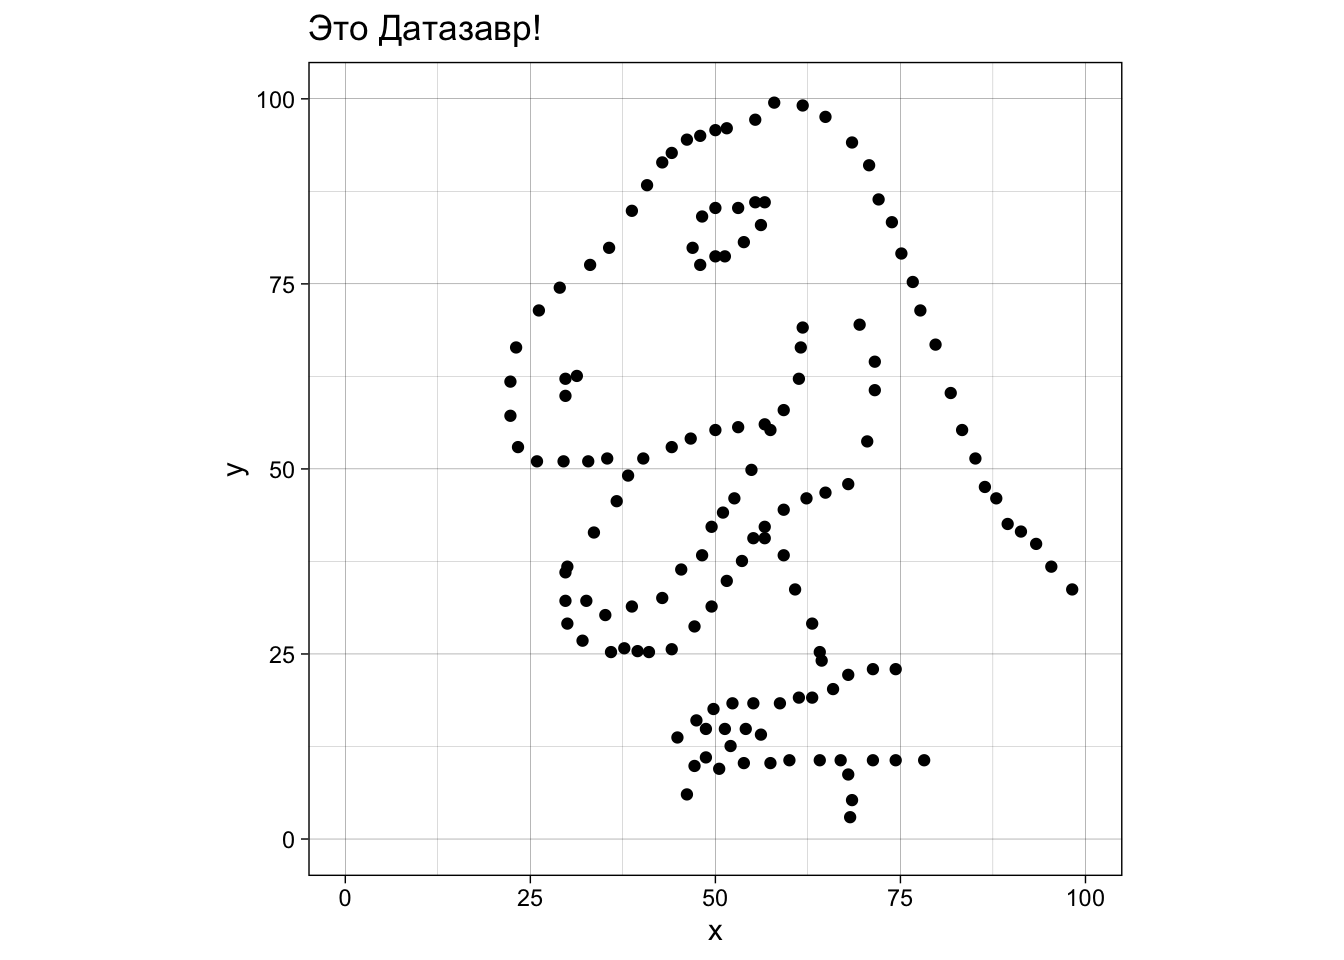
\includegraphics{210-desc_stats_files/figure-pdf/unnamed-chunk-39-1.pdf}

Из этого можно сделать важный вывод: не стоит слепо доверять
описательным статистикам. Нужно визуализировать данные, иначе можно
попасть в такую ситуацию в реальности. По словам знаменитого статитстика
Джона Тьюки, величайшая ценность картинки в том, что она заставляет нас
заметить то, что мы не ожидали заметить. Поэтому графики --- это не
просто метод коммуникации --- представления ваших результатов сообществу
в понятном виде (хотя и это, конечно, тоже), но и сам по себе очень
важный метод анализа данных.

\hypertarget{sec-r_vis}{%
\chapter{Встроенные функции для графиков}\label{sec-r_vis}}

В R есть достаточно мощные встроенные инструменты для визуализации. Я
приведу три простых примера: функции \texttt{plot()}, \texttt{hist()} и
\texttt{boxplot()}.

\hypertarget{sec-base_plot}{%
\section{\texorpdfstring{Многоликий
\texttt{plot()}}{Многоликий plot()}}\label{sec-base_plot}}

Для примера возьмем датасет \texttt{heroes}, вытащим из него колонки
\texttt{Height} и \texttt{Weight} как векторы и применим на них функцию
\texttt{plot()}.

\begin{Shaded}
\begin{Highlighting}[]
\FunctionTok{library}\NormalTok{(}\StringTok{"tidyverse"}\NormalTok{)}
\end{Highlighting}
\end{Shaded}

\begin{verbatim}
-- Attaching packages --------------------------------------- tidyverse 1.3.2 --
v ggplot2 3.4.2     v purrr   1.0.1
v tibble  3.2.1     v dplyr   1.1.2
v tidyr   1.3.0     v stringr 1.5.0
v readr   2.1.3     v forcats 1.0.0
-- Conflicts ------------------------------------------ tidyverse_conflicts() --
x dplyr::filter() masks stats::filter()
x dplyr::lag()    masks stats::lag()
\end{verbatim}

\begin{Shaded}
\begin{Highlighting}[]
\NormalTok{heroes }\OtherTok{\textless{}{-}} \FunctionTok{read\_csv}\NormalTok{(}\StringTok{"https://raw.githubusercontent.com/Pozdniakov/tidy\_stats/master/data/heroes\_information.csv"}\NormalTok{,}
                   \AttributeTok{na =} \FunctionTok{c}\NormalTok{(}\StringTok{"{-}"}\NormalTok{, }\StringTok{"{-}99"}\NormalTok{))}
\end{Highlighting}
\end{Shaded}

\begin{verbatim}
New names:
* `` -> `...1`
\end{verbatim}

\begin{verbatim}
Warning: One or more parsing issues, call `problems()` on your data frame for details,
e.g.:
  dat <- vroom(...)
  problems(dat)
\end{verbatim}

\begin{verbatim}
Rows: 734 Columns: 11
-- Column specification --------------------------------------------------------
Delimiter: ","
chr (8): name, Gender, Eye color, Race, Hair color, Publisher, Skin color, A...
dbl (3): ...1, Height, Weight

i Use `spec()` to retrieve the full column specification for this data.
i Specify the column types or set `show_col_types = FALSE` to quiet this message.
\end{verbatim}

\begin{Shaded}
\begin{Highlighting}[]
\FunctionTok{plot}\NormalTok{(heroes}\SpecialCharTok{$}\NormalTok{Height, heroes}\SpecialCharTok{$}\NormalTok{Weight)}
\end{Highlighting}
\end{Shaded}

\begin{figure}[H]

{\centering 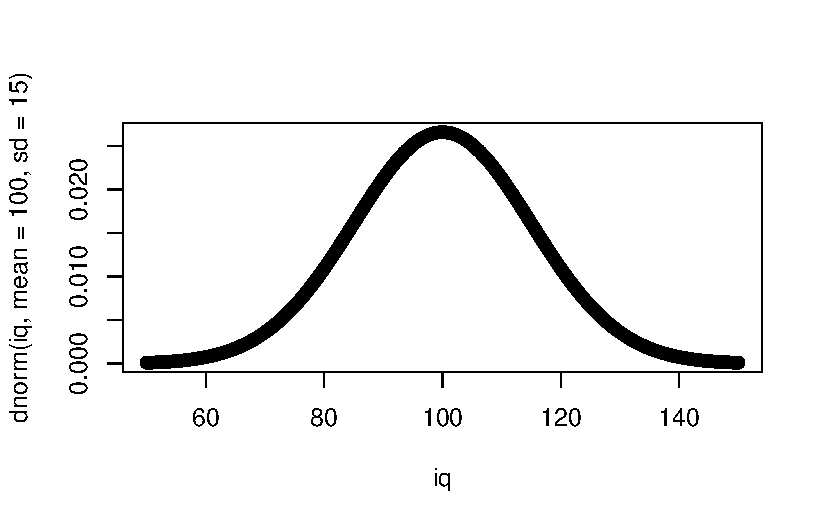
\includegraphics{220-base_viz_files/figure-pdf/unnamed-chunk-2-1.pdf}

}

\end{figure}

В этом случае будет нарисована \textbf{диаграмма рассеяния (точечная
диаграмма, \emph{scatterplot),}} где каждая точка задается парой
значений из этих векторов: значения из колонки \texttt{Height}
используются как координаты по оси \emph{x}, а соответствующие значения
колонки \texttt{Weight} как координаты по оси \emph{y}.

Функция \texttt{plot()} - это тоже \textbf{универсальная
\emph{(generic)}} функция, как и \texttt{summary()}(см.
Глава~\ref{sec-summary}). В качестве аргумента можете ей скормить просто
один вектор, матрицу, датафрейм. Давайте попробуем использовать функцию
\texttt{plot()} на встроенном датафрейме \texttt{iris}\footnote{\texttt{iris}
  -- пожалуй, самый известный набор данных в мире, своего рода
  \emph{``Hello, world!''} от мира науки о данных. Этот датасет был
  собран известным ботаником Эдгаром Андерсоном, но стал известен
  благодаря статье 1936 года известного статистика Роберта Фишера, в
  которой он использовал эти данные для демонстрации разработанного им
  метода дискриминантного анализа. С \texttt{iris} мы еще столкнемся в
  главе про многомерные методы анализа (Глава~\ref{sec-multivar}).}:

\begin{Shaded}
\begin{Highlighting}[]
\NormalTok{iris}
\end{Highlighting}
\end{Shaded}

\begin{verbatim}
    Sepal.Length Sepal.Width Petal.Length Petal.Width    Species
1            5.1         3.5          1.4         0.2     setosa
2            4.9         3.0          1.4         0.2     setosa
3            4.7         3.2          1.3         0.2     setosa
4            4.6         3.1          1.5         0.2     setosa
5            5.0         3.6          1.4         0.2     setosa
6            5.4         3.9          1.7         0.4     setosa
7            4.6         3.4          1.4         0.3     setosa
8            5.0         3.4          1.5         0.2     setosa
9            4.4         2.9          1.4         0.2     setosa
10           4.9         3.1          1.5         0.1     setosa
11           5.4         3.7          1.5         0.2     setosa
12           4.8         3.4          1.6         0.2     setosa
13           4.8         3.0          1.4         0.1     setosa
14           4.3         3.0          1.1         0.1     setosa
15           5.8         4.0          1.2         0.2     setosa
16           5.7         4.4          1.5         0.4     setosa
17           5.4         3.9          1.3         0.4     setosa
18           5.1         3.5          1.4         0.3     setosa
19           5.7         3.8          1.7         0.3     setosa
20           5.1         3.8          1.5         0.3     setosa
21           5.4         3.4          1.7         0.2     setosa
22           5.1         3.7          1.5         0.4     setosa
23           4.6         3.6          1.0         0.2     setosa
24           5.1         3.3          1.7         0.5     setosa
25           4.8         3.4          1.9         0.2     setosa
26           5.0         3.0          1.6         0.2     setosa
27           5.0         3.4          1.6         0.4     setosa
28           5.2         3.5          1.5         0.2     setosa
29           5.2         3.4          1.4         0.2     setosa
30           4.7         3.2          1.6         0.2     setosa
31           4.8         3.1          1.6         0.2     setosa
32           5.4         3.4          1.5         0.4     setosa
33           5.2         4.1          1.5         0.1     setosa
34           5.5         4.2          1.4         0.2     setosa
35           4.9         3.1          1.5         0.2     setosa
36           5.0         3.2          1.2         0.2     setosa
37           5.5         3.5          1.3         0.2     setosa
38           4.9         3.6          1.4         0.1     setosa
39           4.4         3.0          1.3         0.2     setosa
40           5.1         3.4          1.5         0.2     setosa
41           5.0         3.5          1.3         0.3     setosa
42           4.5         2.3          1.3         0.3     setosa
43           4.4         3.2          1.3         0.2     setosa
44           5.0         3.5          1.6         0.6     setosa
45           5.1         3.8          1.9         0.4     setosa
46           4.8         3.0          1.4         0.3     setosa
47           5.1         3.8          1.6         0.2     setosa
48           4.6         3.2          1.4         0.2     setosa
49           5.3         3.7          1.5         0.2     setosa
50           5.0         3.3          1.4         0.2     setosa
51           7.0         3.2          4.7         1.4 versicolor
52           6.4         3.2          4.5         1.5 versicolor
53           6.9         3.1          4.9         1.5 versicolor
54           5.5         2.3          4.0         1.3 versicolor
55           6.5         2.8          4.6         1.5 versicolor
56           5.7         2.8          4.5         1.3 versicolor
57           6.3         3.3          4.7         1.6 versicolor
58           4.9         2.4          3.3         1.0 versicolor
59           6.6         2.9          4.6         1.3 versicolor
60           5.2         2.7          3.9         1.4 versicolor
61           5.0         2.0          3.5         1.0 versicolor
62           5.9         3.0          4.2         1.5 versicolor
63           6.0         2.2          4.0         1.0 versicolor
64           6.1         2.9          4.7         1.4 versicolor
65           5.6         2.9          3.6         1.3 versicolor
66           6.7         3.1          4.4         1.4 versicolor
67           5.6         3.0          4.5         1.5 versicolor
68           5.8         2.7          4.1         1.0 versicolor
69           6.2         2.2          4.5         1.5 versicolor
70           5.6         2.5          3.9         1.1 versicolor
71           5.9         3.2          4.8         1.8 versicolor
72           6.1         2.8          4.0         1.3 versicolor
73           6.3         2.5          4.9         1.5 versicolor
74           6.1         2.8          4.7         1.2 versicolor
75           6.4         2.9          4.3         1.3 versicolor
76           6.6         3.0          4.4         1.4 versicolor
77           6.8         2.8          4.8         1.4 versicolor
78           6.7         3.0          5.0         1.7 versicolor
79           6.0         2.9          4.5         1.5 versicolor
80           5.7         2.6          3.5         1.0 versicolor
81           5.5         2.4          3.8         1.1 versicolor
82           5.5         2.4          3.7         1.0 versicolor
83           5.8         2.7          3.9         1.2 versicolor
84           6.0         2.7          5.1         1.6 versicolor
85           5.4         3.0          4.5         1.5 versicolor
86           6.0         3.4          4.5         1.6 versicolor
87           6.7         3.1          4.7         1.5 versicolor
88           6.3         2.3          4.4         1.3 versicolor
89           5.6         3.0          4.1         1.3 versicolor
90           5.5         2.5          4.0         1.3 versicolor
91           5.5         2.6          4.4         1.2 versicolor
92           6.1         3.0          4.6         1.4 versicolor
93           5.8         2.6          4.0         1.2 versicolor
94           5.0         2.3          3.3         1.0 versicolor
95           5.6         2.7          4.2         1.3 versicolor
96           5.7         3.0          4.2         1.2 versicolor
97           5.7         2.9          4.2         1.3 versicolor
98           6.2         2.9          4.3         1.3 versicolor
99           5.1         2.5          3.0         1.1 versicolor
100          5.7         2.8          4.1         1.3 versicolor
101          6.3         3.3          6.0         2.5  virginica
102          5.8         2.7          5.1         1.9  virginica
103          7.1         3.0          5.9         2.1  virginica
104          6.3         2.9          5.6         1.8  virginica
105          6.5         3.0          5.8         2.2  virginica
106          7.6         3.0          6.6         2.1  virginica
107          4.9         2.5          4.5         1.7  virginica
108          7.3         2.9          6.3         1.8  virginica
109          6.7         2.5          5.8         1.8  virginica
110          7.2         3.6          6.1         2.5  virginica
111          6.5         3.2          5.1         2.0  virginica
112          6.4         2.7          5.3         1.9  virginica
113          6.8         3.0          5.5         2.1  virginica
114          5.7         2.5          5.0         2.0  virginica
115          5.8         2.8          5.1         2.4  virginica
116          6.4         3.2          5.3         2.3  virginica
117          6.5         3.0          5.5         1.8  virginica
118          7.7         3.8          6.7         2.2  virginica
119          7.7         2.6          6.9         2.3  virginica
120          6.0         2.2          5.0         1.5  virginica
121          6.9         3.2          5.7         2.3  virginica
122          5.6         2.8          4.9         2.0  virginica
123          7.7         2.8          6.7         2.0  virginica
124          6.3         2.7          4.9         1.8  virginica
125          6.7         3.3          5.7         2.1  virginica
126          7.2         3.2          6.0         1.8  virginica
127          6.2         2.8          4.8         1.8  virginica
128          6.1         3.0          4.9         1.8  virginica
129          6.4         2.8          5.6         2.1  virginica
130          7.2         3.0          5.8         1.6  virginica
131          7.4         2.8          6.1         1.9  virginica
132          7.9         3.8          6.4         2.0  virginica
133          6.4         2.8          5.6         2.2  virginica
134          6.3         2.8          5.1         1.5  virginica
135          6.1         2.6          5.6         1.4  virginica
136          7.7         3.0          6.1         2.3  virginica
137          6.3         3.4          5.6         2.4  virginica
138          6.4         3.1          5.5         1.8  virginica
139          6.0         3.0          4.8         1.8  virginica
140          6.9         3.1          5.4         2.1  virginica
141          6.7         3.1          5.6         2.4  virginica
142          6.9         3.1          5.1         2.3  virginica
143          5.8         2.7          5.1         1.9  virginica
144          6.8         3.2          5.9         2.3  virginica
145          6.7         3.3          5.7         2.5  virginica
146          6.7         3.0          5.2         2.3  virginica
147          6.3         2.5          5.0         1.9  virginica
148          6.5         3.0          5.2         2.0  virginica
149          6.2         3.4          5.4         2.3  virginica
150          5.9         3.0          5.1         1.8  virginica
\end{verbatim}

Каждая строчка -- один цветок ириса, числовые колонки содержат
информацию о длине и ширине наружной \emph{(sepal)} и внутренней
\emph{(petal)} долях околоцветника, в колонке \texttt{Species}
содержится название сорта ирисов.

Давайте уберем последнюю колонку, чтобы у нас остались только числовые
колонки:

\begin{Shaded}
\begin{Highlighting}[]
\NormalTok{iris[, }\SpecialCharTok{{-}}\DecValTok{5}\NormalTok{]}
\end{Highlighting}
\end{Shaded}

\begin{verbatim}
    Sepal.Length Sepal.Width Petal.Length Petal.Width
1            5.1         3.5          1.4         0.2
2            4.9         3.0          1.4         0.2
3            4.7         3.2          1.3         0.2
4            4.6         3.1          1.5         0.2
5            5.0         3.6          1.4         0.2
6            5.4         3.9          1.7         0.4
7            4.6         3.4          1.4         0.3
8            5.0         3.4          1.5         0.2
9            4.4         2.9          1.4         0.2
10           4.9         3.1          1.5         0.1
11           5.4         3.7          1.5         0.2
12           4.8         3.4          1.6         0.2
13           4.8         3.0          1.4         0.1
14           4.3         3.0          1.1         0.1
15           5.8         4.0          1.2         0.2
16           5.7         4.4          1.5         0.4
17           5.4         3.9          1.3         0.4
18           5.1         3.5          1.4         0.3
19           5.7         3.8          1.7         0.3
20           5.1         3.8          1.5         0.3
21           5.4         3.4          1.7         0.2
22           5.1         3.7          1.5         0.4
23           4.6         3.6          1.0         0.2
24           5.1         3.3          1.7         0.5
25           4.8         3.4          1.9         0.2
26           5.0         3.0          1.6         0.2
27           5.0         3.4          1.6         0.4
28           5.2         3.5          1.5         0.2
29           5.2         3.4          1.4         0.2
30           4.7         3.2          1.6         0.2
31           4.8         3.1          1.6         0.2
32           5.4         3.4          1.5         0.4
33           5.2         4.1          1.5         0.1
34           5.5         4.2          1.4         0.2
35           4.9         3.1          1.5         0.2
36           5.0         3.2          1.2         0.2
37           5.5         3.5          1.3         0.2
38           4.9         3.6          1.4         0.1
39           4.4         3.0          1.3         0.2
40           5.1         3.4          1.5         0.2
41           5.0         3.5          1.3         0.3
42           4.5         2.3          1.3         0.3
43           4.4         3.2          1.3         0.2
44           5.0         3.5          1.6         0.6
45           5.1         3.8          1.9         0.4
46           4.8         3.0          1.4         0.3
47           5.1         3.8          1.6         0.2
48           4.6         3.2          1.4         0.2
49           5.3         3.7          1.5         0.2
50           5.0         3.3          1.4         0.2
51           7.0         3.2          4.7         1.4
52           6.4         3.2          4.5         1.5
53           6.9         3.1          4.9         1.5
54           5.5         2.3          4.0         1.3
55           6.5         2.8          4.6         1.5
56           5.7         2.8          4.5         1.3
57           6.3         3.3          4.7         1.6
58           4.9         2.4          3.3         1.0
59           6.6         2.9          4.6         1.3
60           5.2         2.7          3.9         1.4
61           5.0         2.0          3.5         1.0
62           5.9         3.0          4.2         1.5
63           6.0         2.2          4.0         1.0
64           6.1         2.9          4.7         1.4
65           5.6         2.9          3.6         1.3
66           6.7         3.1          4.4         1.4
67           5.6         3.0          4.5         1.5
68           5.8         2.7          4.1         1.0
69           6.2         2.2          4.5         1.5
70           5.6         2.5          3.9         1.1
71           5.9         3.2          4.8         1.8
72           6.1         2.8          4.0         1.3
73           6.3         2.5          4.9         1.5
74           6.1         2.8          4.7         1.2
75           6.4         2.9          4.3         1.3
76           6.6         3.0          4.4         1.4
77           6.8         2.8          4.8         1.4
78           6.7         3.0          5.0         1.7
79           6.0         2.9          4.5         1.5
80           5.7         2.6          3.5         1.0
81           5.5         2.4          3.8         1.1
82           5.5         2.4          3.7         1.0
83           5.8         2.7          3.9         1.2
84           6.0         2.7          5.1         1.6
85           5.4         3.0          4.5         1.5
86           6.0         3.4          4.5         1.6
87           6.7         3.1          4.7         1.5
88           6.3         2.3          4.4         1.3
89           5.6         3.0          4.1         1.3
90           5.5         2.5          4.0         1.3
91           5.5         2.6          4.4         1.2
92           6.1         3.0          4.6         1.4
93           5.8         2.6          4.0         1.2
94           5.0         2.3          3.3         1.0
95           5.6         2.7          4.2         1.3
96           5.7         3.0          4.2         1.2
97           5.7         2.9          4.2         1.3
98           6.2         2.9          4.3         1.3
99           5.1         2.5          3.0         1.1
100          5.7         2.8          4.1         1.3
101          6.3         3.3          6.0         2.5
102          5.8         2.7          5.1         1.9
103          7.1         3.0          5.9         2.1
104          6.3         2.9          5.6         1.8
105          6.5         3.0          5.8         2.2
106          7.6         3.0          6.6         2.1
107          4.9         2.5          4.5         1.7
108          7.3         2.9          6.3         1.8
109          6.7         2.5          5.8         1.8
110          7.2         3.6          6.1         2.5
111          6.5         3.2          5.1         2.0
112          6.4         2.7          5.3         1.9
113          6.8         3.0          5.5         2.1
114          5.7         2.5          5.0         2.0
115          5.8         2.8          5.1         2.4
116          6.4         3.2          5.3         2.3
117          6.5         3.0          5.5         1.8
118          7.7         3.8          6.7         2.2
119          7.7         2.6          6.9         2.3
120          6.0         2.2          5.0         1.5
121          6.9         3.2          5.7         2.3
122          5.6         2.8          4.9         2.0
123          7.7         2.8          6.7         2.0
124          6.3         2.7          4.9         1.8
125          6.7         3.3          5.7         2.1
126          7.2         3.2          6.0         1.8
127          6.2         2.8          4.8         1.8
128          6.1         3.0          4.9         1.8
129          6.4         2.8          5.6         2.1
130          7.2         3.0          5.8         1.6
131          7.4         2.8          6.1         1.9
132          7.9         3.8          6.4         2.0
133          6.4         2.8          5.6         2.2
134          6.3         2.8          5.1         1.5
135          6.1         2.6          5.6         1.4
136          7.7         3.0          6.1         2.3
137          6.3         3.4          5.6         2.4
138          6.4         3.1          5.5         1.8
139          6.0         3.0          4.8         1.8
140          6.9         3.1          5.4         2.1
141          6.7         3.1          5.6         2.4
142          6.9         3.1          5.1         2.3
143          5.8         2.7          5.1         1.9
144          6.8         3.2          5.9         2.3
145          6.7         3.3          5.7         2.5
146          6.7         3.0          5.2         2.3
147          6.3         2.5          5.0         1.9
148          6.5         3.0          5.2         2.0
149          6.2         3.4          5.4         2.3
150          5.9         3.0          5.1         1.8
\end{verbatim}

\begin{Shaded}
\begin{Highlighting}[]
\FunctionTok{plot}\NormalTok{(iris[, }\SpecialCharTok{{-}}\DecValTok{5}\NormalTok{])}
\end{Highlighting}
\end{Shaded}

\begin{figure}[H]

{\centering \includegraphics{220-base_viz_files/figure-pdf/unnamed-chunk-5-1.pdf}

}

\end{figure}

Мы получили таблицу из \textbf{диаграмм рассеяния!} Для каждой пары
колонок строится отдельная диаграмма рассеяния, что может быть очень
удобно при исследовании данных.

Многие пакеты добавляют новые методы \texttt{plot()} для объектов из
новых классов, поэтому функцию \texttt{plot()} имеет смысл пробовать на
любых непривычных вам объектах.

\hypertarget{sec-base_vis_hist}{%
\section{Великая гистограмма}\label{sec-base_vis_hist}}

Другая распространенная функция --- \texttt{hist()} ---
\textbf{гистограмма (histogram)}:

\begin{Shaded}
\begin{Highlighting}[]
\NormalTok{weight }\OtherTok{\textless{}{-}}\NormalTok{ heroes }\SpecialCharTok{\%\textgreater{}\%}
  \FunctionTok{drop\_na}\NormalTok{(Weight) }\SpecialCharTok{\%\textgreater{}\%}
  \FunctionTok{pull}\NormalTok{(Weight)}
\FunctionTok{hist}\NormalTok{(weight)}
\end{Highlighting}
\end{Shaded}

\begin{figure}[H]

{\centering \includegraphics{220-base_viz_files/figure-pdf/unnamed-chunk-6-1.pdf}

}

\end{figure}

Гистограмма -- очень простая визуализация, которую при желании несложно
нарисовать карандашом на бумаге, следуя простому алгоритму:

\begin{enumerate}
\def\labelenumi{\arabic{enumi}.}
\tightlist
\item
  Весь диапазон значений в выборке делим на интервалы (обычно
  одинаковые, но можно и разные).
\item
  Считаем сколько точек попадает в каждый из интервалов.
\item
  Откладываем высоту столбцов в зависимости от количества точек в каждом
  интервале.
\end{enumerate}

Главный вопрос здесь: на какие интервалы мы делим? В зависимости от
этого гистограмма может выглядеть очень по-разному.

Количество интервалов можно задать самостоятельно с помощью аргумента
\texttt{breaks\ =}:

\begin{Shaded}
\begin{Highlighting}[]
\FunctionTok{hist}\NormalTok{(weight, }\AttributeTok{breaks =} \DecValTok{4}\NormalTok{)}
\end{Highlighting}
\end{Shaded}

\begin{figure}[H]

{\centering \includegraphics{220-base_viz_files/figure-pdf/unnamed-chunk-7-1.pdf}

}

\end{figure}

\begin{Shaded}
\begin{Highlighting}[]
\FunctionTok{hist}\NormalTok{(weight, }\AttributeTok{breaks =} \DecValTok{30}\NormalTok{)}
\end{Highlighting}
\end{Shaded}

\begin{figure}[H]

{\centering \includegraphics{220-base_viz_files/figure-pdf/unnamed-chunk-8-1.pdf}

}

\end{figure}

\begin{Shaded}
\begin{Highlighting}[]
\FunctionTok{hist}\NormalTok{(weight, }\AttributeTok{breaks =} \DecValTok{100}\NormalTok{)}
\end{Highlighting}
\end{Shaded}

\begin{figure}[H]

{\centering \includegraphics{220-base_viz_files/figure-pdf/unnamed-chunk-9-1.pdf}

}

\end{figure}

Попробовав различные значения, можно убедиться, что форма гистограммы
может достаточно сильно изменяться в зависимости от выбранного
количества интервалов\footnote{На самом деле, функция \texttt{hist()}
  будет использовать заданное количество интервал очень ориентировочно:
  на основе желаемого количества интервалов будут вычисляться интервалы
  с круглыми границами.}.

\begin{tcolorbox}[enhanced jigsaw, leftrule=.75mm, toprule=.15mm, left=2mm, breakable, arc=.35mm, rightrule=.15mm, colback=white, opacityback=0, bottomrule=.15mm]

\textbf{\emph{Для продвинутых:} правило Стёрджеса и иже с
ними}\vspace{2mm}

По умолчанию, функция \texttt{hist()} использует
\href{https://ru.wikipedia.org/wiki/Правило_Стёрджеса}{\textbf{правило
Стёрджеса}} \textbf{\emph{(Sturges' rule)}} для определения количества
интервалов гистограммы:
\[\displaystyle n=1+\lfloor \log _{2}N\rfloor\]Здесь \(N\) -- размер
выборки, а \(\lfloor \rfloor\) обозначают целую часть числа (т.е.
округление вниз). Если мы возьмем вектор \texttt{weight}, длина которого
495, то получим 9 интервалов:

\begin{Shaded}
\begin{Highlighting}[]
\DecValTok{1} \SpecialCharTok{+} \FunctionTok{floor}\NormalTok{(}\FunctionTok{log}\NormalTok{(}\FunctionTok{length}\NormalTok{(weight), }\AttributeTok{base =} \DecValTok{2}\NormalTok{))}
\end{Highlighting}
\end{Shaded}

\begin{verbatim}
[1] 9
\end{verbatim}

Правило Стёрджеса -- только один из алгоритмов для расчета количества
интервалов в гистограмме! Есть и множество других, например,
\textbf{правило Фридмана-Диакониса \emph{(Freedman--Diaconis' rule)}} и
\textbf{правило Скотта \emph{(Scott's normal reference rule).}} Чтобы
ими воспользоваться в функции \texttt{hist()}, нужно прописать
\texttt{breaks\ =\ "FD"} или \texttt{"Scott"} соответственно.

\end{tcolorbox}

\hypertarget{sec-base_vis_boxplot}{%
\section{Нестареющий боксплот}\label{sec-base_vis_boxplot}}

Ну и закончим на суперзвезде прошлого века под названием \textbf{ящик с
усами \emph{(boxplot with whiskers):}}

\begin{Shaded}
\begin{Highlighting}[]
\FunctionTok{boxplot}\NormalTok{(Weight }\SpecialCharTok{\textasciitilde{}}\NormalTok{ Gender, heroes)}
\end{Highlighting}
\end{Shaded}

\begin{figure}[H]

{\centering 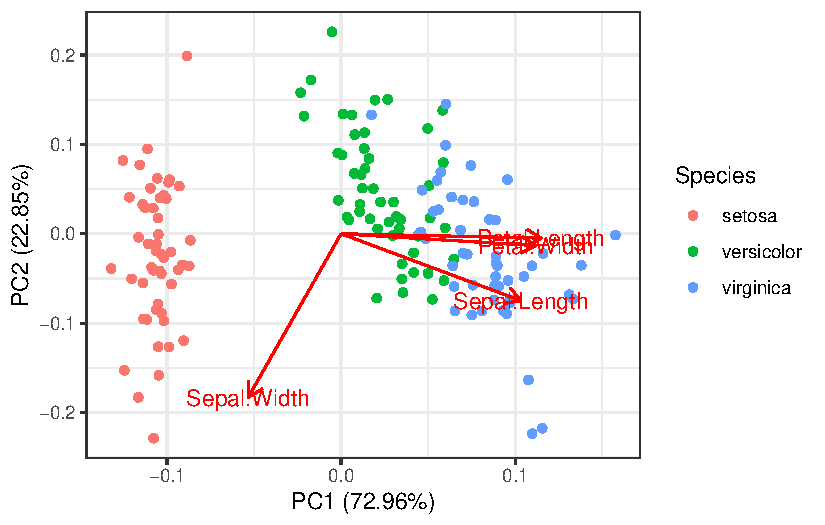
\includegraphics{220-base_viz_files/figure-pdf/unnamed-chunk-11-1.pdf}

}

\end{figure}

Здесь мы использовали уже знакомый нам класс формул. Они еще будут нам
встречаться дальше, обычно они используются следующим образом: слева от
\texttt{\textasciitilde{}} находится зависимая переменная, а справа -
``предикторы''. Эта интуиция работает и здесь: мы хотим посмотреть, как
различается вес в зависимости от пола.

Несмотря на свою популярность, ящик с усами -- достаточно непростой тип
графиков. С одной стороны, он неплохо помогает понять, как распределены
данные. С другой стороны, немногие знают, как эти ящики и усы рисуются.

Начнем с линии в середине ящика -- это медиана (а не среднее, как могло
бы показаться). Низ и верх ящика -- это Q1 и Q3 соответственно. А это
значит, что высота ящика -- это разница между Q1 и Q3, т.е.
межквартильный размах.

А вот с усами все еще сложнее. Они строятся следующим образом: от края
ящика откладываются полтора межквартильных размаха. Но ус рисуется не на
этой границе (1.5 IQR), а по крайней точке внутри полутора
межквартильных размахов. Если остаются значения за пределами полутора
межквартильных размахов, то они отмечаются точками.

Очень часто эти точки называют ``выбросами'', однако это может запутать:
нет никакого магического алгоритма, который назначает эти точки
выбросами. Точнее, алгоритм есть (и мы его теперь знаем), но в нем нет
никакой магии. Почему именно квартили и медиана? А, главное, почему
именно полтора межквартильных размаха? Просто так решили. Могли бы взять
и 1, и 2, и 1.4, и 1.645 межквартильных размаха, просто потому что (а
еще число 1.5 -- число более красивое, чем в 1.4 и 1.645). Это может
показаться удивительным, что в статистике, области математики,
используются взятые с потолка числа, но скоро мы убедимся, что такое
встречается сплошь и рядом.

\hypertarget{ux437ux430ux43aux43bux44eux447ux435ux43dux438ux435}{%
\section{Заключение}\label{ux437ux430ux43aux43bux44eux447ux435ux43dux438ux435}}

Возможности R для визуализации очень богатые, и некоторые даже
утверждают, что их
\href{https://flowingdata.com/2016/03/22/comparing-ggplot2-and-r-base-graphics/}{более
чем достаточно}. Главное преимущество встроенных функций для графики в R
-- возможность быстро нарисовать простой график с помощью одной функции,
не подключая никаких дополнительных пакетов. Это делает базовые функции
визуализации в R удобными для исследования данных.

\hypertarget{sec-gg_ggplot2}{%
\chapter{\texorpdfstring{Грамматика графики
\texttt{ggplot2}}{Грамматика графики ggplot2}}\label{sec-gg_ggplot2}}

\hypertarget{sec-grammar_of_graphics}{%
\section{История грамматики графики}\label{sec-grammar_of_graphics}}

Встроенные возможности для визуализации в R довольно обширны, но
дополнительные пакеты значительно ее расширяют. Среди этих пакетов, есть
один, который занимает совершенно особенное место -- \texttt{ggplot2}.

\texttt{ggplot2} --- это не просто пакет, который рисует красивые
графики. Красивые графики можно рисовать и в базовом R. Чтобы понять,
почему пакет \texttt{ggplot2} занимает особенное место среди пакетов для
визуализации (и не только среди пакетов для R, а вообще!), нужно
расшифровать \texttt{gg} в его названии. \texttt{gg} означает грамматику
графики (Grammar of Graphics), язык для описания графиков, изложенный в
одноименной книге Леланда Уилкинсона (Wilkinson 2005).

Грамматика графики позволяет описывать графики не в терминах типологии
(вот есть пайчарт, есть барплот, есть гистограмма, а есть ящик с усами),
а с помощью специального разработанного языка. Этот язык позволяет с
помощью грамматики и небольшого количества ``слов'' языка описывать и
создавать практически любые графики и даже придумывать новые! Это дает
огромную свободу в создании именно той визуализации, что необходима для
текущей задачи.

Хэдли Уикхэм (да, снова он) немного дополнил идею грамматики графики в
статье ``A Layered grammar of graphics'' (Wickham 2010), которую
сопроводил пакетом \texttt{ggplot2} с реализацией идей Уилкинсона и
своих.

\hypertarget{sec-gg_base}{%
\section{Основы грамматики графики}\label{sec-gg_base}}

Каждый график состоит из одного или нескольких \textbf{слоев (layers)}.
Если слоев несколько, то они располагаются один над другим, при этом
верхние слои ``перекрывают'' нижние, примерно как это происходит в
программах вроде Adobe Photoshop. У каждого слоя есть три обязательных
элемента: \textbf{данные (data)}, \textbf{геом (geom)}, \textbf{эстетики
(aestetics)}; и два вспомогательных: \textbf{статистические
трансформации (stat).} и \textbf{регулировка положения (position
adjustment).}

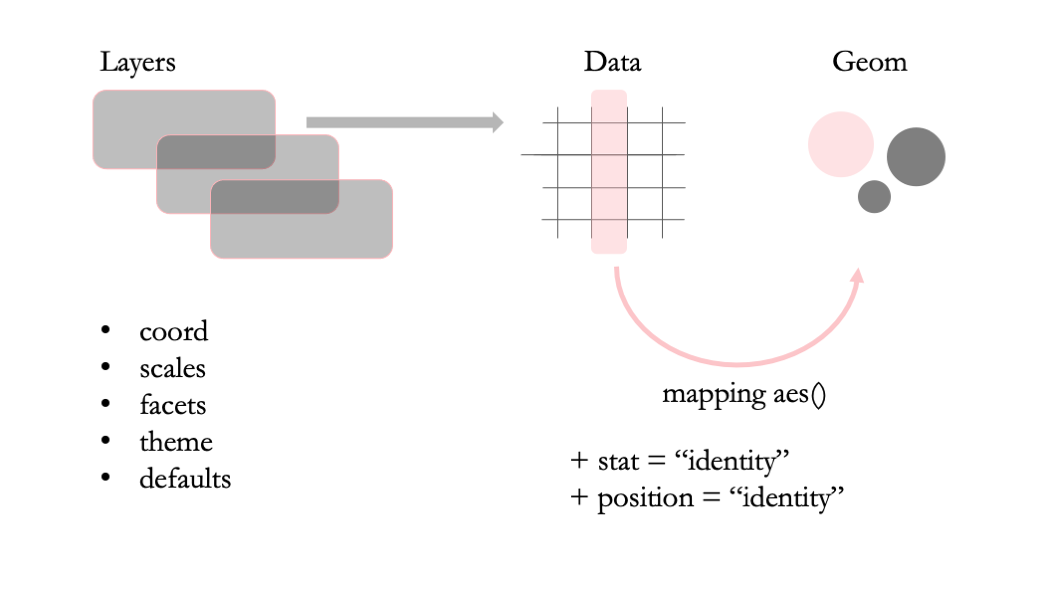
\includegraphics{images/ggplot2_scheme.png}

\begin{itemize}
\item
  \textbf{Данные (data).} Собственно, сами данные в виде датафрейма,
  используемые в данном слое.
\item
  \textbf{Геом (geom).} Геом --- это сокращение от ``геометрический
  объект''. Собственно, в какой геометрический объект мы собираемся
  превращать данные. Например, в точки, прямоугольники или линии.
\item
  \textbf{Отображение (mapping).} Эстетические отображения или просто
  \textbf{эстетики (aestetics)} --- это набор правил, как различные
  переменные превращаются в визуальные особенности геометрии. Без
  эстетик остается непонятно, какие именно колонки в используемом
  датафрейме превращаются в различные особенности геомов: позицию,
  размер, цвет и т.д. У каждой геометрии свой набор эстетик, но многие
  из них совпадают у разных геомов, например, \emph{x}, \emph{y},
  \emph{colour}, \emph{fill}, \emph{size}. Без некоторых эстетик геом не
  будет работать. Например, геометрия в виде точек не будет работать без
  двух координат этих точек (\emph{x} и \emph{y}). Другие эстетики
  необязательны и имеют значения по умолчанию. Например, по умолчанию
  точки будут черными, но можно сделать их цвет зависимым от выбранной
  колонки в датафрейме с помощью эстетики \emph{colour}.
\item
  \textbf{Статистические трансформации (stat).} Название используемой
  статистической трансформации (или просто --- статистики). Да,
  статистические трансформации можно делать прямо внутри
  \texttt{ggplot2}! Это дает дополнительную свободу в выборе
  инструментов, потому что обычно те же статистические трансформации
  можно сделать вне \texttt{ggplot2} в процессе препроцессинга.
  Формально, статистические трансформации --- это обязательный элемент
  геома, но если вы не хотите преобразовывать данные, то можете выбрать
  ``identity'' преобразование, которое оставляет все как есть. В
  \texttt{ggplot2} у каждого геома есть статистика по умолчанию, а у
  каждой статистики - свой геом по умолчанию. И не всегда статистика по
  умолчанию --- это ``identity'' статистика. Например, для барплота
  (\texttt{geom\_barplot()}) используется статистика ``count''
  \footnote{идентична по своему смыслу функции \texttt{dplyr::count},
    которая считает частоты по выбранной колонке тиббла
    @ref(tidy\_count)}, которая считает частоты, ведь именно частоты
  затем трансформируются в высоту барплотов.
\end{itemize}

\begin{itemize}
\tightlist
\item
  \textbf{Регулировка положения (position adjustment).} Регуляровка
  положения --- это небольшое улучшение позиции геометрий для части
  элементов. Например, можно добавить немного случайного шума
  (``jitter'') в позицию точек, чтобы они не перекрывали друг друга. Или
  ``раздвинуть'' (``dodge'') два барплота, чтобы один не загораживал
  другой. Как и в случае со статистическими трансформациями, в
  большинстве случаев значение по умолчанию --- ``identity''.
\end{itemize}

Кроме слоев, у графика есть:

\begin{itemize}
\tightlist
\item
  \textbf{Координатная система (coord).} Если мы задали координаты, то
  нам нужно задать и координатную плоскость, верно? Конечно, в
  большинстве случаев используется \emph{декартова система координат
  (Cartesian coordinate system)} \footnote{Декартова система координат
    названа в честь великого математика и философа Рене Декарта, на
    латинском --- \emph{Renatus Cartesius}, отсюда и название
    \emph{cartesian coordinate system}.}, т.е. стандартная прямоугольная
  система координат, но можно использовать и другие, например, полярную
  систему координат или картографическую проекцию.
\end{itemize}

\begin{itemize}
\item
  \textbf{Шкалы (scales).} Шкалы задают то, \emph{как именно} значения
  превращаются в эстетики. Например, если мы задали, что разные значения
  в колонке будут влиять на цвет точки, то какая именно палитра будет
  использоваться? В какие конкретно цвета будут превращаться числовые,
  логические или строковые значения в колонке? В \texttt{ggplot2} есть
  правила по умолчанию для всех эстестик, и они отличные, но
  самостоятельная настройка шкал может значительно улучшить график.
\item
  \textbf{Фасетки (facets).} Фасетки --- это одно из нововведений
  Уикхэма в грамматику графики. Фасетки повзоляют разбить график на
  множество похожих, задав переменную, по которой график будет разделен.
  Это очень напоминает использование группировки с помощью
  \texttt{group\_by()}.
\item
  \textbf{Тема (theme).} Тема --- это зрительное оформление ``подложки''
  графика, не относящийся к содержанию графика: размер шрифта, цвет
  фона, размер и цвет линий на фоне и т.д. и т.п. В \texttt{ggplot2}
  есть несколько встроенных тем, а также есть множество пакетов, которые
  добавляют дополнительные темы. Кроме того, их можно настраивать
  самостоятельно!
\item
  \textbf{Значения по умолчанию (defaults).} Если в графике используется
  несколько слоев, то часто все они используют одни и те же данные и
  эстетики. Можно задать данные и эстетики по умолчанию для всего
  графика, чтобы не повторять код.
\end{itemize}

\hypertarget{sec-gg_0}{%
\section{Пример №0: пайчарт с распределение по полу}\label{sec-gg_0}}

Сейчас мы попробуем сделать простой пример в \texttt{ggplot2}, похожий
на пример, который использует в своей книге Леланд Уилкинсон, чтобы
показать мощь грамматики графики (Wilkinson 2005). Приготовьтесь, этот
пример перевернет ваши представления о графиках!

Но сначала взглянем на структуру кода в \texttt{ggplot()}.

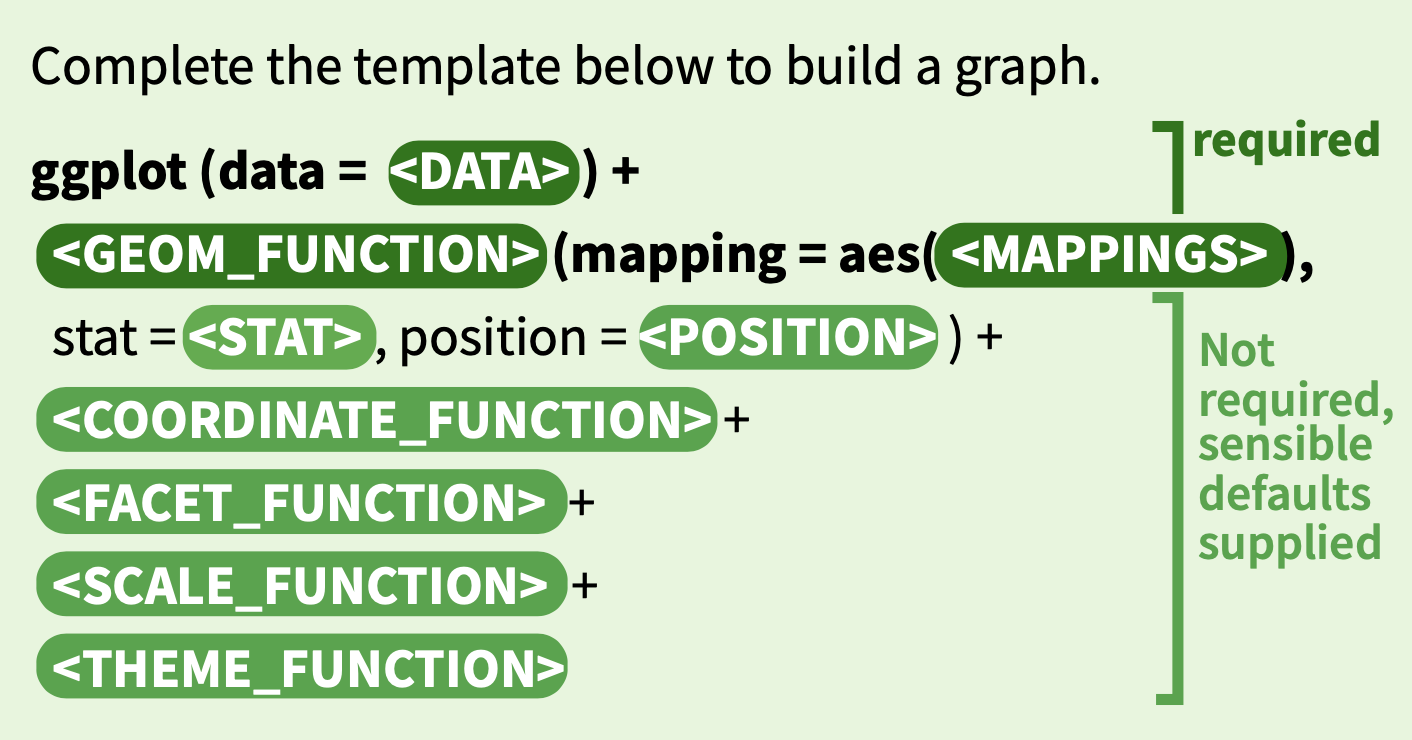
\includegraphics[width=4.16667in,height=\textheight]{images/ggplot_code.png}

Как видно, код чем-то напоминает стандартный код tidyverse, но с
\texttt{+} вместо пайпов. Когда был написан \texttt{ggplot2}, Хэдли
Уикхэм еще не знал про \texttt{\%\textgreater{}\%} из \texttt{magrittr},
хотя по смыслу \texttt{+} означает примерно то же самое.

\begin{Shaded}
\begin{Highlighting}[]
\FunctionTok{library}\NormalTok{(tidyverse)}
\end{Highlighting}
\end{Shaded}

\begin{verbatim}
-- Attaching packages --------------------------------------- tidyverse 1.3.2 --
v ggplot2 3.4.2     v purrr   1.0.1
v tibble  3.2.1     v dplyr   1.1.2
v tidyr   1.3.0     v stringr 1.5.0
v readr   2.1.3     v forcats 1.0.0
-- Conflicts ------------------------------------------ tidyverse_conflicts() --
x dplyr::filter() masks stats::filter()
x dplyr::lag()    masks stats::lag()
\end{verbatim}

\begin{Shaded}
\begin{Highlighting}[]
\NormalTok{heroes }\OtherTok{\textless{}{-}} \FunctionTok{read\_csv}\NormalTok{(}\StringTok{"https://raw.githubusercontent.com/Pozdniakov/tidy\_stats/master/data/heroes\_information.csv"}\NormalTok{,}
                   \AttributeTok{na =} \FunctionTok{c}\NormalTok{(}\StringTok{"{-}"}\NormalTok{, }\StringTok{"{-}99"}\NormalTok{))}
\end{Highlighting}
\end{Shaded}

\begin{verbatim}
New names:
* `` -> `...1`
\end{verbatim}

\begin{verbatim}
Warning: One or more parsing issues, call `problems()` on your data frame for details,
e.g.:
  dat <- vroom(...)
  problems(dat)
\end{verbatim}

\begin{verbatim}
Rows: 734 Columns: 11
-- Column specification --------------------------------------------------------
Delimiter: ","
chr (8): name, Gender, Eye color, Race, Hair color, Publisher, Skin color, A...
dbl (3): ...1, Height, Weight

i Use `spec()` to retrieve the full column specification for this data.
i Specify the column types or set `show_col_types = FALSE` to quiet this message.
\end{verbatim}

Итак, запустим функцию \texttt{ggplot()}, задав наш тиббл
\texttt{heroes} в качестве данных.

\begin{Shaded}
\begin{Highlighting}[]
\FunctionTok{ggplot}\NormalTok{(}\AttributeTok{data =}\NormalTok{ heroes)}
\end{Highlighting}
\end{Shaded}

\begin{figure}[H]

{\centering 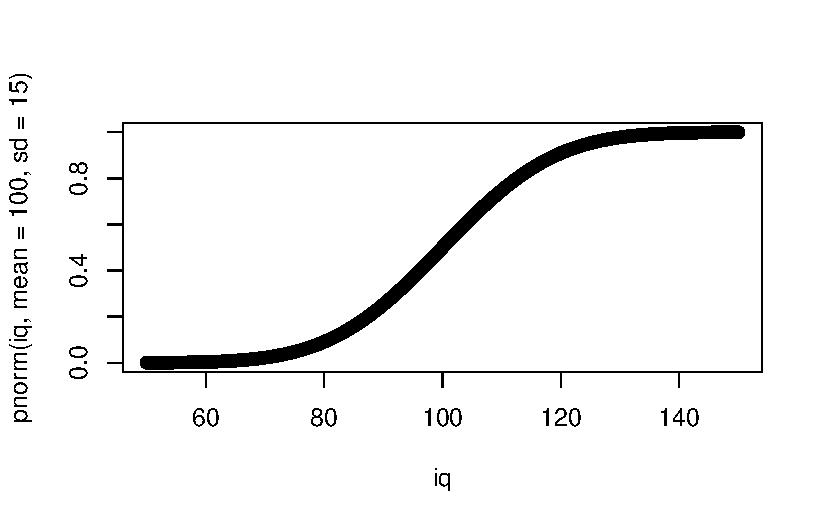
\includegraphics{230-ggplot2_files/figure-pdf/unnamed-chunk-3-1.pdf}

}

\end{figure}

Мы ничего не получили! Это естественно, ведь мы задали только данные по
умолчанию, но не задали геометрию и эстетики.

Функция \texttt{ggplot()} не просто отрисовывает график, эта функция
создает объект класса \texttt{ggplot}, который можно сохранить и
модифицировать в дальнейшем:

\begin{Shaded}
\begin{Highlighting}[]
\NormalTok{almost\_empty\_ggplot }\OtherTok{\textless{}{-}} \FunctionTok{ggplot}\NormalTok{(}\AttributeTok{data =}\NormalTok{ heroes)}
\NormalTok{almost\_empty\_ggplot}
\end{Highlighting}
\end{Shaded}

\begin{figure}[H]

{\centering 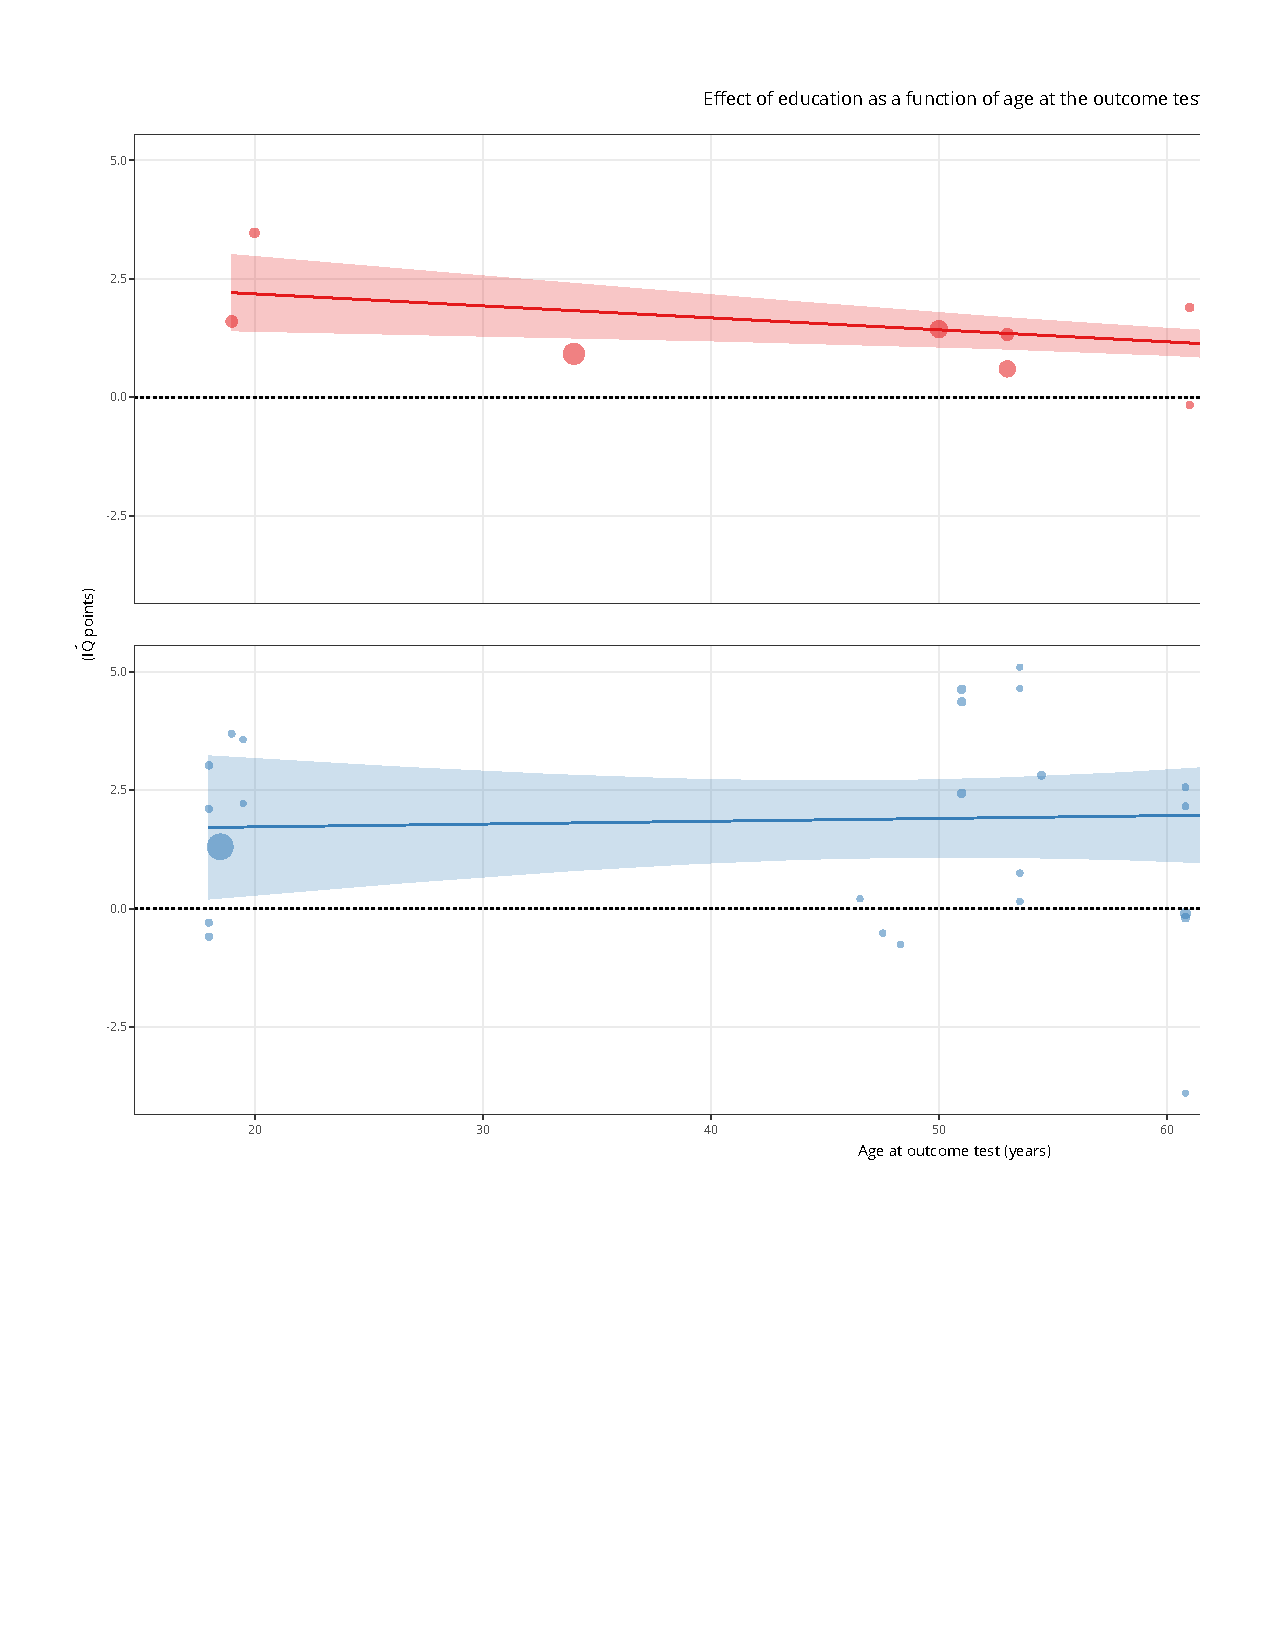
\includegraphics{230-ggplot2_files/figure-pdf/unnamed-chunk-4-1.pdf}

}

\end{figure}

Возьмем \texttt{geom\_bar()} для отрисовки барплота. В качестве эстетик
поставим \texttt{x\ =\ Gender} и \texttt{fill\ =\ Gender}. Поскольку это
эстетики, они обозначаются внутри функции параметра
\texttt{mapping\ =\ aes()} или просто внутри функции \texttt{aes()}. По
умолчанию, \texttt{geom\_bar()} имеет статистику ``count'', что нас
полностью устраивает: \texttt{geom\_bar()} сам посчитает табличу частот
и использует значения \texttt{Gender} для обозначения позиций и заливки,
а посчитанные частоты будет использовать для задания высоты столбцов.

\begin{Shaded}
\begin{Highlighting}[]
\FunctionTok{ggplot}\NormalTok{(}\AttributeTok{data =}\NormalTok{ heroes) }\SpecialCharTok{+}
  \FunctionTok{geom\_bar}\NormalTok{(}\FunctionTok{aes}\NormalTok{(}\AttributeTok{x =}\NormalTok{ Gender, }\AttributeTok{fill =}\NormalTok{ Gender))}
\end{Highlighting}
\end{Shaded}

\begin{figure}[H]

{\centering \includegraphics{230-ggplot2_files/figure-pdf/unnamed-chunk-5-1.pdf}

}

\end{figure}

Сейчас мы сделаем один хитрый трюк: поставим значение эстетики
\texttt{x\ =\ ""}, чтобы собрать все столбики в один.

\begin{Shaded}
\begin{Highlighting}[]
\FunctionTok{ggplot}\NormalTok{(}\AttributeTok{data =}\NormalTok{ heroes) }\SpecialCharTok{+}
  \FunctionTok{geom\_bar}\NormalTok{(}\FunctionTok{aes}\NormalTok{(}\AttributeTok{x =} \StringTok{""}\NormalTok{, }\AttributeTok{fill =}\NormalTok{ Gender))}
\end{Highlighting}
\end{Shaded}

\begin{figure}[H]

{\centering \includegraphics{230-ggplot2_files/figure-pdf/unnamed-chunk-6-1.pdf}

}

\end{figure}

Получилось что-то не очень симпатичное, но вполне осмысленное: доли
столбца обозначают относительную частоту.

Можно настроить общие параметры геома, не зависящие от данных. Это нужно
делать \emph{вне} функции \texttt{aes()}, но внутри функции для геома.

\begin{Shaded}
\begin{Highlighting}[]
\FunctionTok{ggplot}\NormalTok{(}\AttributeTok{data =}\NormalTok{ heroes) }\SpecialCharTok{+}
  \FunctionTok{geom\_bar}\NormalTok{(}\FunctionTok{aes}\NormalTok{(}\AttributeTok{x =} \StringTok{""}\NormalTok{, }\AttributeTok{fill =}\NormalTok{ Gender), }\AttributeTok{width =}\NormalTok{ .}\DecValTok{2}\NormalTok{)}
\end{Highlighting}
\end{Shaded}

\begin{figure}[H]

{\centering \includegraphics{230-ggplot2_files/figure-pdf/unnamed-chunk-7-1.pdf}

}

\end{figure}

\begin{quote}
Казалось бы, причем здесь Minecraft?
\end{quote}

А теперь внимание! Подумайте, какого действия нам не хватает, чтобы из
имеющегося графика получить пайчарт?

\begin{Shaded}
\begin{Highlighting}[]
\FunctionTok{ggplot}\NormalTok{(}\AttributeTok{data =}\NormalTok{ heroes) }\SpecialCharTok{+}
  \FunctionTok{geom\_bar}\NormalTok{(}\FunctionTok{aes}\NormalTok{(}\AttributeTok{x =} \StringTok{""}\NormalTok{, }\AttributeTok{fill =}\NormalTok{ Gender)) }\SpecialCharTok{+}
  \FunctionTok{coord\_polar}\NormalTok{(}\AttributeTok{theta =} \StringTok{"y"}\NormalTok{)}
\end{Highlighting}
\end{Shaded}

\begin{figure}[H]

{\centering \includegraphics{230-ggplot2_files/figure-pdf/unnamed-chunk-8-1.pdf}

}

\end{figure}

Нам нужно было всего-лишь поменять систему координат с декартовой на
полярную (круговую)! Иначе говоря, пайчарт - это барплот в полярной
системе координат.

Именно в этом основная сила грамматики графики и ее реализации в
\texttt{ggplot2} --- вместо того, чтобы описывать и рисовать огромное
количество типов графиков, можно описать практически любой график через
небольшой количество элементарных элементов и правила их соединения.

Получившийся пайчарт осталось подретушировать, убрав все лишние элементы
подложки с помощью самой минималистичной темы \texttt{theme\_void()} и
добавив название графика:

\begin{Shaded}
\begin{Highlighting}[]
\FunctionTok{ggplot}\NormalTok{(}\AttributeTok{data =}\NormalTok{ heroes) }\SpecialCharTok{+}
  \FunctionTok{geom\_bar}\NormalTok{(}\FunctionTok{aes}\NormalTok{(}\AttributeTok{x =} \StringTok{""}\NormalTok{, }\AttributeTok{fill =}\NormalTok{ Gender)) }\SpecialCharTok{+}
  \FunctionTok{coord\_polar}\NormalTok{(}\AttributeTok{theta =} \StringTok{"y"}\NormalTok{) }\SpecialCharTok{+}
  \FunctionTok{theme\_void}\NormalTok{() }\SpecialCharTok{+}
  \FunctionTok{labs}\NormalTok{(}\AttributeTok{title =} \StringTok{"Gender distributions for superheroes"}\NormalTok{)}
\end{Highlighting}
\end{Shaded}

\begin{figure}[H]

{\centering \includegraphics{230-ggplot2_files/figure-pdf/unnamed-chunk-9-1.pdf}

}

\end{figure}

Это был интересный, но немного шуточный пример. Все-таки пайчарт --- это
довольно спорный способ визуализировать данные, вызывающий много вполне
справедливой критики. Поэтому сейчас мы перейдем к гораздо более
реалистичному примеру.

\hypertarget{sec-gg_1}{%
\section{Пример №1: Education and IQ meta-analysis}\label{sec-gg_1}}

Для этого примера мы возьмем мета-анализ связи количества лет обучения и
интеллекта: \emph{``How Much Does Education Improve Intelligence? A
Meta-Analysis''} (Ritchie и Tucker-Drob 2018). Мета-анализ --- это
группа статистических методов, которые позволяют объединить результаты
нескольких исследований с похожим планом исследованием и тематикой,
чтобы посчитать средний эффект между несколькими статьями сразу.

Данные и скрипт для анализа данных в этой статье находятся в открытом
доступе: https://osf.io/r8a24/

Полный текст статьи доступен по
\href{https://www.ncbi.nlm.nih.gov/pmc/articles/PMC6088505/}{ссылке}.

Существует положительная корреляция между количеством лет, который
человек потратил на обучение, и интеллектом. Это может объясняться
по-разному: как то, что обучение повышает интеллект, и как то, что люди
с высоким интеллекте стремятся получать больше образования. Напрямую в
эксперименте это проверить нельзя, поэтому есть несколько
квази-экспериментальных планов, которые косвенно указывают на верность
той или иной гипотезу. Например, если в стране изменилось количество лет
обязательного школьного образования, то повлияло ли это на интеллект
целого поколения? \sout{Или все-таки дело в Моргенштерне}

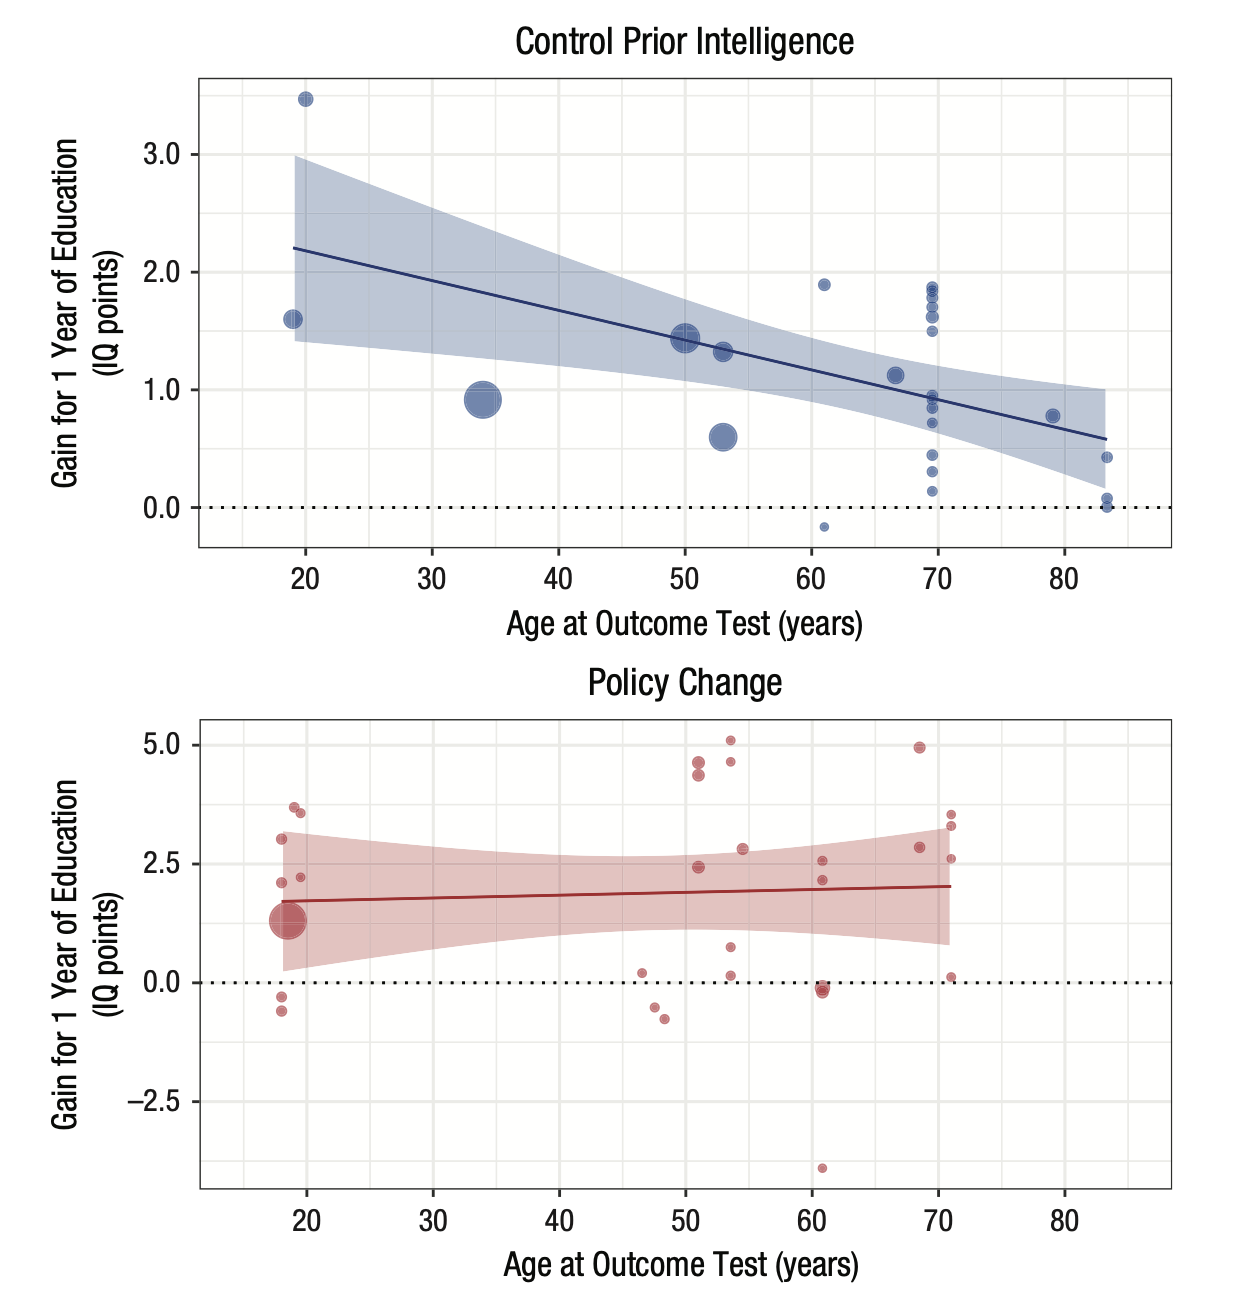
\includegraphics{images/meta_2.png}

Данная картинка показывает, насколько размер эффекта (выраженный в
баллах IQ) зависит от того, какой средний возраст участвоваших в
исследовании испытуемых.

Каждая точка на этом графике --- это отдельное исследование, положение
по оси \emph{x} --- средний возраст респондентов, а положение по оси
\emph{y} - средний прирост интеллекта согласно исследованию. Размер
точки отражает ``точность'' исследования (грубо говоря, чем больше
выборка, тем больше точка). Два графика обозначают два
квазиэкспериментальных плана.

Мы сфокусируемся на нижней картинке с ``Policy change'' --- это как раз
исследования, в которых изучается изменения интеллекта в возрастных
группах после изменения количества лет обучения в школе.

Мы полностью воспроизведем код построчно, посмотрим, как эта картинка
создавалась шаг за шагом.

Заметьте, данный датасет использует немного непривычный для нас формат
хранения данных. Попытайтесь самостоятельно прочитать его.

\begin{Shaded}
\begin{Highlighting}[]
\FunctionTok{library}\NormalTok{(tidyverse)}
\NormalTok{df }\OtherTok{\textless{}{-}} \FunctionTok{read\_tsv}\NormalTok{(}\StringTok{"https://raw.githubusercontent.com/Pozdniakov/tidy\_stats/master/data/meta\_dataset.txt"}\NormalTok{)}
\end{Highlighting}
\end{Shaded}

\begin{verbatim}
Rows: 142 Columns: 17
-- Column specification --------------------------------------------------------
Delimiter: "\t"
chr  (2): Country, Design
dbl (15): Study_ID, Data_ID, k, n, outcome_test_cat, Effect_size, SE, Outcom...

i Use `spec()` to retrieve the full column specification for this data.
i Specify the column types or set `show_col_types = FALSE` to quiet this message.
\end{verbatim}

Давайте посмотрим, как устроен датафрейм \texttt{df}:

\begin{Shaded}
\begin{Highlighting}[]
\NormalTok{df}
\end{Highlighting}
\end{Shaded}

\begin{verbatim}
# A tibble: 142 x 17
   Study_ID Data_ID     k Country     n Design      outcome_test_cat Effect_size
      <dbl>   <dbl> <dbl> <chr>   <dbl> <chr>                  <dbl>       <dbl>
 1      1         1     4 UK        483 Control Pr~                0     0.778  
 2      1         1     4 UK        290 Control Pr~                1     0.0771 
 3      1         1     4 UK        290 Control Pr~                1     0.427  
 4      1         1     4 UK        288 Control Pr~                1     0.00519
 5      1         2    13 UK       1017 Control Pr~                0     1.62   
 6      1         2    13 UK       1022 Control Pr~                1     0.915  
 7      1         2    13 UK       1021 Control Pr~                1     0.305  
 8      1         2    13 UK        981 Control Pr~                1     0.719  
 9      1.5       2    13 UK       1024 Control Pr~                1     1.70   
10      1.5       2    13 UK       1023 Control Pr~                1     1.78   
# i 132 more rows
# i 9 more variables: SE <dbl>, Outcome_age <dbl>, quasi_age <dbl>,
#   cpiq_early_age <dbl>, cpiq_age_diff <dbl>, ses_funnel <dbl>,
#   published <dbl>, Male_only <dbl>, Achievement <dbl>
\end{verbatim}

Каждая строчка --- это результат отдельного исследования, при этом одна
статья может включать несколько исследований,

В дальнейшем мы будем использовать код авторов статьи и смотреть,
строчка за строчкой, как он будет работать.

\begin{Shaded}
\begin{Highlighting}[]
\NormalTok{cpiq }\OtherTok{\textless{}{-}} \FunctionTok{subset}\NormalTok{(df, }\AttributeTok{subset=}\NormalTok{(Design}\SpecialCharTok{==}\StringTok{"Control Prior IQ"}\NormalTok{))}
\NormalTok{poli }\OtherTok{\textless{}{-}} \FunctionTok{subset}\NormalTok{(df, }\AttributeTok{subset=}\NormalTok{(Design}\SpecialCharTok{==}\StringTok{"Policy Change"}\NormalTok{))}
\end{Highlighting}
\end{Shaded}

Авторы исследования используют \texttt{subset()}, это функция базового
R, принцип которой очень похож на \texttt{filter()} \footnote{Кстати,
  именно функция \texttt{subset()} вдохновила Уикхема на создание
  \texttt{filter()}.}.

Итак, начнем рисовать сам график. Сначала иницируем объект
\texttt{ggplot} с данными \texttt{poli} по умолчанию.

\begin{Shaded}
\begin{Highlighting}[]
\FunctionTok{ggplot}\NormalTok{(}\AttributeTok{data=}\NormalTok{poli) }
\end{Highlighting}
\end{Shaded}

\begin{figure}[H]

{\centering 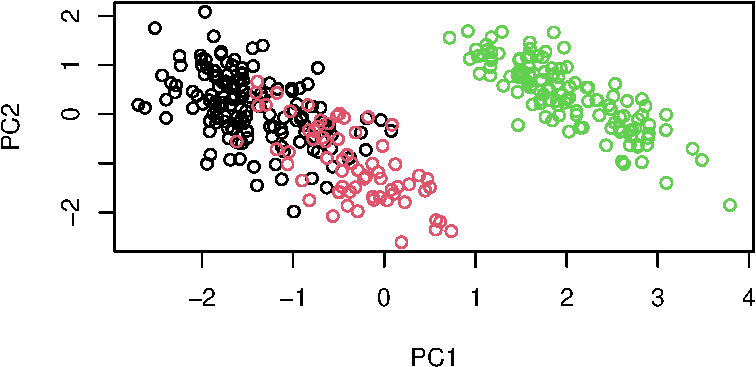
\includegraphics{230-ggplot2_files/figure-pdf/unnamed-chunk-13-1.pdf}

}

\end{figure}

Теперь добавим в качестве эстетик по умолчанию координаты:
\texttt{aes(x=Outcome\_age,\ y=Effect\_size)}.

\begin{Shaded}
\begin{Highlighting}[]
\FunctionTok{ggplot}\NormalTok{(}\FunctionTok{aes}\NormalTok{(}\AttributeTok{x=}\NormalTok{Outcome\_age, }\AttributeTok{y=}\NormalTok{Effect\_size), }\AttributeTok{data=}\NormalTok{poli) }
\end{Highlighting}
\end{Shaded}

\begin{figure}[H]

{\centering 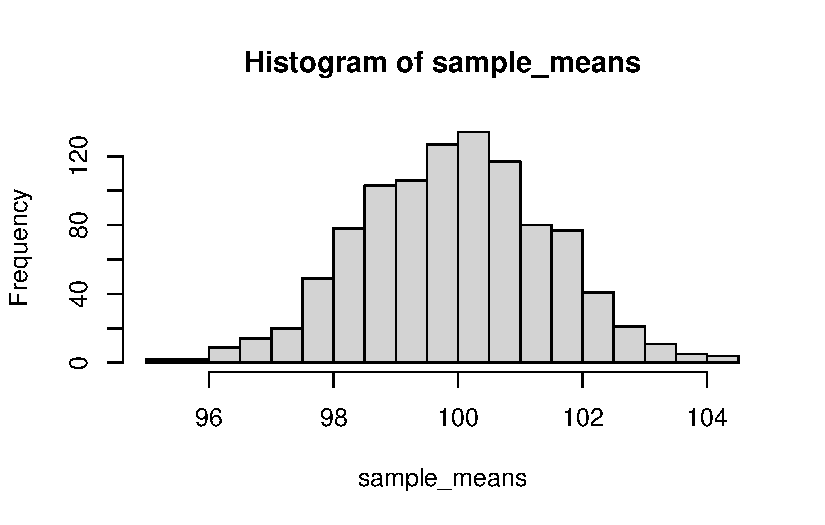
\includegraphics{230-ggplot2_files/figure-pdf/unnamed-chunk-14-1.pdf}

}

\end{figure}

Что изменилось? Появилась координатная ось и шкалы. Заметьте, масштаб
неслучаен: он строится на основе разброса значений в выбранных колонках.
Однако этого недостаточно для отрисовки графика, нехватает геометрии:
нужно задать, в какую географическую сущность отобразятся данные.

\begin{Shaded}
\begin{Highlighting}[]
\FunctionTok{ggplot}\NormalTok{(}\FunctionTok{aes}\NormalTok{(}\AttributeTok{x=}\NormalTok{Outcome\_age, }\AttributeTok{y=}\NormalTok{Effect\_size), }\AttributeTok{data=}\NormalTok{poli) }\SpecialCharTok{+}
        \FunctionTok{geom\_point}\NormalTok{() }
\end{Highlighting}
\end{Shaded}

\begin{figure}[H]

{\centering \includegraphics{230-ggplot2_files/figure-pdf/unnamed-chunk-15-1.pdf}

}

\end{figure}

Готово! Это и есть основа картинки. Добавляем размер:

\begin{Shaded}
\begin{Highlighting}[]
\FunctionTok{ggplot}\NormalTok{(}\FunctionTok{aes}\NormalTok{(}\AttributeTok{x=}\NormalTok{Outcome\_age, }\AttributeTok{y=}\NormalTok{Effect\_size, }\AttributeTok{size=}\DecValTok{1}\SpecialCharTok{/}\NormalTok{(SE}\SpecialCharTok{\^{}}\DecValTok{2}\NormalTok{)), }\AttributeTok{data=}\NormalTok{poli) }\SpecialCharTok{+}
        \FunctionTok{geom\_point}\NormalTok{() }
\end{Highlighting}
\end{Shaded}

\begin{figure}[H]

{\centering \includegraphics{230-ggplot2_files/figure-pdf/unnamed-chunk-16-1.pdf}

}

\end{figure}

Перед нами возникла проблема оверплоттинга: некоторые точки перекрывают
друг друга, поскольку имеют очень близкие координат. Авторы графика
решают эту проблему очевидным способом: добавляют прозрачности точкам.
Заметьте, прозрачность задается для всех точек одним значением, поэтому
параметр \texttt{alpha} задается вне функции \texttt{aes()}.

\begin{Shaded}
\begin{Highlighting}[]
\FunctionTok{ggplot}\NormalTok{(}\FunctionTok{aes}\NormalTok{(}\AttributeTok{x=}\NormalTok{Outcome\_age, }\AttributeTok{y=}\NormalTok{Effect\_size, }\AttributeTok{size=}\DecValTok{1}\SpecialCharTok{/}\NormalTok{(SE}\SpecialCharTok{\^{}}\DecValTok{2}\NormalTok{)), }\AttributeTok{data=}\NormalTok{poli) }\SpecialCharTok{+}
        \FunctionTok{geom\_point}\NormalTok{(}\AttributeTok{alpha=}\NormalTok{.}\DecValTok{55}\NormalTok{) }
\end{Highlighting}
\end{Shaded}

\begin{figure}[H]

{\centering \includegraphics{230-ggplot2_files/figure-pdf/unnamed-chunk-17-1.pdf}

}

\end{figure}

Совершенно так же задается и цвет. Он задается одинаковым для всех точек
с помощью \href{https://ru.wikipedia.org/wiki/Цвета_HTML}{HEX-кода}.

\begin{Shaded}
\begin{Highlighting}[]
\FunctionTok{ggplot}\NormalTok{(}\FunctionTok{aes}\NormalTok{(}\AttributeTok{x=}\NormalTok{Outcome\_age, }\AttributeTok{y=}\NormalTok{Effect\_size, }\AttributeTok{size=}\DecValTok{1}\SpecialCharTok{/}\NormalTok{(SE}\SpecialCharTok{\^{}}\DecValTok{2}\NormalTok{)), }\AttributeTok{data=}\NormalTok{poli) }\SpecialCharTok{+}
        \FunctionTok{geom\_point}\NormalTok{(}\AttributeTok{alpha=}\NormalTok{.}\DecValTok{55}\NormalTok{, }\AttributeTok{colour=}\StringTok{"\#BA1825"}\NormalTok{)}
\end{Highlighting}
\end{Shaded}

\begin{figure}[H]

{\centering \includegraphics{230-ggplot2_files/figure-pdf/unnamed-chunk-18-1.pdf}

}

\end{figure}

Теперь добавим регрессионную прямую с доверительными интервалами на
график. Это специальный геом \texttt{geom\_smooth()} со специальной
статистикой, который займет второй слой данного графика.

\begin{Shaded}
\begin{Highlighting}[]
\FunctionTok{ggplot}\NormalTok{(}\FunctionTok{aes}\NormalTok{(}\AttributeTok{x=}\NormalTok{Outcome\_age, }\AttributeTok{y=}\NormalTok{Effect\_size, }\AttributeTok{size=}\DecValTok{1}\SpecialCharTok{/}\NormalTok{(SE}\SpecialCharTok{\^{}}\DecValTok{2}\NormalTok{)), }\AttributeTok{data=}\NormalTok{poli) }\SpecialCharTok{+}
        \FunctionTok{geom\_point}\NormalTok{(}\AttributeTok{alpha=}\NormalTok{.}\DecValTok{55}\NormalTok{, }\AttributeTok{colour=}\StringTok{"\#BA1825"}\NormalTok{) }\SpecialCharTok{+}
        \FunctionTok{geom\_smooth}\NormalTok{()}
\end{Highlighting}
\end{Shaded}

\begin{verbatim}
Warning: Using `size` aesthetic for lines was deprecated in ggplot2 3.4.0.
i Please use `linewidth` instead.
\end{verbatim}

\begin{verbatim}
`geom_smooth()` using method = 'loess' and formula = 'y ~ x'
\end{verbatim}

\begin{verbatim}
Warning: The following aesthetics were dropped during statistical transformation: size
i This can happen when ggplot fails to infer the correct grouping structure in
  the data.
i Did you forget to specify a `group` aesthetic or to convert a numerical
  variable into a factor?
\end{verbatim}

\begin{figure}[H]

{\centering \includegraphics{230-ggplot2_files/figure-pdf/unnamed-chunk-19-1.pdf}

}

\end{figure}

По умолчанию \texttt{geom\_smooth()} строит кривую линию. Поставим
\texttt{method\ =\ "lm"} для прямой.

\begin{Shaded}
\begin{Highlighting}[]
\FunctionTok{ggplot}\NormalTok{(}\FunctionTok{aes}\NormalTok{(}\AttributeTok{x=}\NormalTok{Outcome\_age, }\AttributeTok{y=}\NormalTok{Effect\_size, }\AttributeTok{size=}\DecValTok{1}\SpecialCharTok{/}\NormalTok{(SE}\SpecialCharTok{\^{}}\DecValTok{2}\NormalTok{)), }\AttributeTok{data=}\NormalTok{poli) }\SpecialCharTok{+}
        \FunctionTok{geom\_point}\NormalTok{(}\AttributeTok{alpha=}\NormalTok{.}\DecValTok{55}\NormalTok{, }\AttributeTok{colour=}\StringTok{"\#BA1825"}\NormalTok{) }\SpecialCharTok{+}
        \FunctionTok{geom\_smooth}\NormalTok{(}\AttributeTok{method=}\StringTok{"lm"}\NormalTok{)}
\end{Highlighting}
\end{Shaded}

\begin{verbatim}
`geom_smooth()` using formula = 'y ~ x'
\end{verbatim}

\begin{verbatim}
Warning: The following aesthetics were dropped during statistical transformation: size
i This can happen when ggplot fails to infer the correct grouping structure in
  the data.
i Did you forget to specify a `group` aesthetic or to convert a numerical
  variable into a factor?
\end{verbatim}

\begin{figure}[H]

{\centering \includegraphics{230-ggplot2_files/figure-pdf/unnamed-chunk-20-1.pdf}

}

\end{figure}

Теперь нужно поменять цвет: ярко синий цвет, используемый по умолчанию
здесь попросту мешает восприятию графика.

\begin{Shaded}
\begin{Highlighting}[]
\FunctionTok{ggplot}\NormalTok{(}\FunctionTok{aes}\NormalTok{(}\AttributeTok{x=}\NormalTok{Outcome\_age, }\AttributeTok{y=}\NormalTok{Effect\_size, }\AttributeTok{size=}\DecValTok{1}\SpecialCharTok{/}\NormalTok{(SE}\SpecialCharTok{\^{}}\DecValTok{2}\NormalTok{)), }\AttributeTok{data=}\NormalTok{poli) }\SpecialCharTok{+}
        \FunctionTok{geom\_point}\NormalTok{(}\AttributeTok{alpha=}\NormalTok{.}\DecValTok{55}\NormalTok{, }\AttributeTok{colour=}\StringTok{"\#BA1825"}\NormalTok{) }\SpecialCharTok{+}
        \FunctionTok{geom\_smooth}\NormalTok{(}\AttributeTok{method=}\StringTok{"lm"}\NormalTok{, }\AttributeTok{colour=}\StringTok{"\#BA1825"}\NormalTok{)}
\end{Highlighting}
\end{Shaded}

\begin{verbatim}
`geom_smooth()` using formula = 'y ~ x'
\end{verbatim}

\begin{verbatim}
Warning: The following aesthetics were dropped during statistical transformation: size
i This can happen when ggplot fails to infer the correct grouping structure in
  the data.
i Did you forget to specify a `group` aesthetic or to convert a numerical
  variable into a factor?
\end{verbatim}

\begin{figure}[H]

{\centering \includegraphics{230-ggplot2_files/figure-pdf/unnamed-chunk-21-1.pdf}

}

\end{figure}

Авторы графика перекрашивают серую полупрозначную область тоже. В этом
случае используется параметр \texttt{fill\ =}, а не \texttt{colour\ =},
но цвет используется тот же.

\begin{Shaded}
\begin{Highlighting}[]
\FunctionTok{ggplot}\NormalTok{(}\FunctionTok{aes}\NormalTok{(}\AttributeTok{x=}\NormalTok{Outcome\_age, }\AttributeTok{y=}\NormalTok{Effect\_size, }\AttributeTok{size=}\DecValTok{1}\SpecialCharTok{/}\NormalTok{(SE}\SpecialCharTok{\^{}}\DecValTok{2}\NormalTok{)), }\AttributeTok{data=}\NormalTok{poli) }\SpecialCharTok{+}
        \FunctionTok{geom\_point}\NormalTok{(}\AttributeTok{alpha=}\NormalTok{.}\DecValTok{55}\NormalTok{, }\AttributeTok{colour=}\StringTok{"\#BA1825"}\NormalTok{) }\SpecialCharTok{+}
        \FunctionTok{geom\_smooth}\NormalTok{(}\AttributeTok{method=}\StringTok{"lm"}\NormalTok{, }\AttributeTok{colour=}\StringTok{"\#BA1825"}\NormalTok{,}\AttributeTok{fill=}\StringTok{"\#BA1825"}\NormalTok{)}
\end{Highlighting}
\end{Shaded}

\begin{verbatim}
`geom_smooth()` using formula = 'y ~ x'
\end{verbatim}

\begin{verbatim}
Warning: The following aesthetics were dropped during statistical transformation: size
i This can happen when ggplot fails to infer the correct grouping structure in
  the data.
i Did you forget to specify a `group` aesthetic or to convert a numerical
  variable into a factor?
\end{verbatim}

\begin{figure}[H]

{\centering \includegraphics{230-ggplot2_files/figure-pdf/unnamed-chunk-22-1.pdf}

}

\end{figure}

Регрессионную линию авторы немного утоньшают с помощью параметра
\texttt{size\ =}.

\begin{Shaded}
\begin{Highlighting}[]
\FunctionTok{ggplot}\NormalTok{(}\FunctionTok{aes}\NormalTok{(}\AttributeTok{x=}\NormalTok{Outcome\_age, }\AttributeTok{y=}\NormalTok{Effect\_size, }\AttributeTok{size=}\DecValTok{1}\SpecialCharTok{/}\NormalTok{(SE}\SpecialCharTok{\^{}}\DecValTok{2}\NormalTok{)), }\AttributeTok{data=}\NormalTok{poli) }\SpecialCharTok{+}
        \FunctionTok{geom\_point}\NormalTok{(}\AttributeTok{alpha=}\NormalTok{.}\DecValTok{55}\NormalTok{, }\AttributeTok{colour=}\StringTok{"\#BA1825"}\NormalTok{) }\SpecialCharTok{+}
        \FunctionTok{geom\_smooth}\NormalTok{(}\AttributeTok{method=}\StringTok{"lm"}\NormalTok{, }\AttributeTok{colour=}\StringTok{"\#BA1825"}\NormalTok{,}\AttributeTok{fill=}\StringTok{"\#BA1825"}\NormalTok{,}\AttributeTok{size=}\NormalTok{.}\DecValTok{5}\NormalTok{)}
\end{Highlighting}
\end{Shaded}

\begin{verbatim}
`geom_smooth()` using formula = 'y ~ x'
\end{verbatim}

\begin{figure}[H]

{\centering \includegraphics{230-ggplot2_files/figure-pdf/unnamed-chunk-23-1.pdf}

}

\end{figure}

Чтобы сместить фокус в сторону точек, авторы добавляют прозрачности для
всего \texttt{geom\_smooth()}.

\begin{Shaded}
\begin{Highlighting}[]
\FunctionTok{ggplot}\NormalTok{(}\FunctionTok{aes}\NormalTok{(}\AttributeTok{x=}\NormalTok{Outcome\_age, }\AttributeTok{y=}\NormalTok{Effect\_size, }\AttributeTok{size=}\DecValTok{1}\SpecialCharTok{/}\NormalTok{(SE}\SpecialCharTok{\^{}}\DecValTok{2}\NormalTok{)), }\AttributeTok{data=}\NormalTok{poli) }\SpecialCharTok{+}
        \FunctionTok{geom\_point}\NormalTok{(}\AttributeTok{alpha=}\NormalTok{.}\DecValTok{55}\NormalTok{, }\AttributeTok{colour=}\StringTok{"\#BA1825"}\NormalTok{) }\SpecialCharTok{+}
        \FunctionTok{geom\_smooth}\NormalTok{(}\AttributeTok{method=}\StringTok{"lm"}\NormalTok{, }\AttributeTok{colour=}\StringTok{"\#BA1825"}\NormalTok{,}\AttributeTok{fill=}\StringTok{"\#BA1825"}\NormalTok{,}\AttributeTok{size=}\NormalTok{.}\DecValTok{5}\NormalTok{, }\AttributeTok{alpha=}\NormalTok{.}\DecValTok{25}\NormalTok{)}
\end{Highlighting}
\end{Shaded}

\begin{verbatim}
`geom_smooth()` using formula = 'y ~ x'
\end{verbatim}

\begin{figure}[H]

{\centering \includegraphics{230-ggplot2_files/figure-pdf/unnamed-chunk-24-1.pdf}

}

\end{figure}

На шкале присутствует 0, и по умолчанию он никак не обозначен. Это легко
исправить с помощью вспомогательного геома \texttt{geom\_hline()}.

\begin{Shaded}
\begin{Highlighting}[]
\FunctionTok{ggplot}\NormalTok{(}\FunctionTok{aes}\NormalTok{(}\AttributeTok{x=}\NormalTok{Outcome\_age, }\AttributeTok{y=}\NormalTok{Effect\_size, }\AttributeTok{size=}\DecValTok{1}\SpecialCharTok{/}\NormalTok{(SE}\SpecialCharTok{\^{}}\DecValTok{2}\NormalTok{)), }\AttributeTok{data=}\NormalTok{poli) }\SpecialCharTok{+}
        \FunctionTok{geom\_point}\NormalTok{(}\AttributeTok{alpha=}\NormalTok{.}\DecValTok{55}\NormalTok{, }\AttributeTok{colour=}\StringTok{"\#BA1825"}\NormalTok{) }\SpecialCharTok{+}
        \FunctionTok{geom\_hline}\NormalTok{(}\AttributeTok{yintercept=}\DecValTok{0}\NormalTok{) }\SpecialCharTok{+} 
        \FunctionTok{geom\_smooth}\NormalTok{(}\AttributeTok{method=}\StringTok{"lm"}\NormalTok{, }\AttributeTok{colour=}\StringTok{"\#BA1825"}\NormalTok{,}\AttributeTok{fill=}\StringTok{"\#BA1825"}\NormalTok{,}\AttributeTok{size=}\NormalTok{.}\DecValTok{5}\NormalTok{, }\AttributeTok{alpha=}\NormalTok{.}\DecValTok{25}\NormalTok{)}
\end{Highlighting}
\end{Shaded}

\begin{verbatim}
`geom_smooth()` using formula = 'y ~ x'
\end{verbatim}

\begin{figure}[H]

{\centering \includegraphics{230-ggplot2_files/figure-pdf/unnamed-chunk-25-1.pdf}

}

\end{figure}

Оттенить эту линию можно, сделав ее пунктирной.

\begin{Shaded}
\begin{Highlighting}[]
\FunctionTok{ggplot}\NormalTok{(}\FunctionTok{aes}\NormalTok{(}\AttributeTok{x=}\NormalTok{Outcome\_age, }\AttributeTok{y=}\NormalTok{Effect\_size, }\AttributeTok{size=}\DecValTok{1}\SpecialCharTok{/}\NormalTok{(SE}\SpecialCharTok{\^{}}\DecValTok{2}\NormalTok{)), }\AttributeTok{data=}\NormalTok{poli) }\SpecialCharTok{+}
        \FunctionTok{geom\_point}\NormalTok{(}\AttributeTok{alpha=}\NormalTok{.}\DecValTok{55}\NormalTok{, }\AttributeTok{colour=}\StringTok{"\#BA1825"}\NormalTok{) }\SpecialCharTok{+}
        \FunctionTok{geom\_hline}\NormalTok{(}\AttributeTok{yintercept=}\DecValTok{0}\NormalTok{, }\AttributeTok{linetype=}\StringTok{"dotted"}\NormalTok{) }\SpecialCharTok{+} 
        \FunctionTok{geom\_smooth}\NormalTok{(}\AttributeTok{method=}\StringTok{"lm"}\NormalTok{, }\AttributeTok{colour=}\StringTok{"\#BA1825"}\NormalTok{,}\AttributeTok{fill=}\StringTok{"\#BA1825"}\NormalTok{,}\AttributeTok{size=}\NormalTok{.}\DecValTok{5}\NormalTok{, }\AttributeTok{alpha=}\NormalTok{.}\DecValTok{25}\NormalTok{)}
\end{Highlighting}
\end{Shaded}

\begin{verbatim}
`geom_smooth()` using formula = 'y ~ x'
\end{verbatim}

\begin{figure}[H]

{\centering \includegraphics{230-ggplot2_files/figure-pdf/unnamed-chunk-26-1.pdf}

}

\end{figure}

Авторы графика вручную задают деления шкалы по оси \emph{x}.

\begin{Shaded}
\begin{Highlighting}[]
\FunctionTok{ggplot}\NormalTok{(}\FunctionTok{aes}\NormalTok{(}\AttributeTok{x=}\NormalTok{Outcome\_age, }\AttributeTok{y=}\NormalTok{Effect\_size, }\AttributeTok{size=}\DecValTok{1}\SpecialCharTok{/}\NormalTok{(SE}\SpecialCharTok{\^{}}\DecValTok{2}\NormalTok{)), }\AttributeTok{data=}\NormalTok{poli) }\SpecialCharTok{+}
        \FunctionTok{geom\_point}\NormalTok{(}\AttributeTok{alpha=}\NormalTok{.}\DecValTok{55}\NormalTok{, }\AttributeTok{colour=}\StringTok{"\#BA1825"}\NormalTok{) }\SpecialCharTok{+}
        \FunctionTok{geom\_hline}\NormalTok{(}\AttributeTok{yintercept=}\DecValTok{0}\NormalTok{, }\AttributeTok{linetype=}\StringTok{"dotted"}\NormalTok{) }\SpecialCharTok{+} 
        \FunctionTok{scale\_x\_continuous}\NormalTok{(}\AttributeTok{breaks=}\FunctionTok{c}\NormalTok{(}\DecValTok{20}\NormalTok{,}\DecValTok{30}\NormalTok{,}\DecValTok{40}\NormalTok{,}\DecValTok{50}\NormalTok{,}\DecValTok{60}\NormalTok{,}\DecValTok{70}\NormalTok{,}\DecValTok{80}\NormalTok{)) }\SpecialCharTok{+}
        \FunctionTok{geom\_smooth}\NormalTok{(}\AttributeTok{method=}\StringTok{"lm"}\NormalTok{, }\AttributeTok{colour=}\StringTok{"\#BA1825"}\NormalTok{,}\AttributeTok{fill=}\StringTok{"\#BA1825"}\NormalTok{,}\AttributeTok{size=}\NormalTok{.}\DecValTok{5}\NormalTok{, }\AttributeTok{alpha=}\NormalTok{.}\DecValTok{25}\NormalTok{)}
\end{Highlighting}
\end{Shaded}

\begin{verbatim}
`geom_smooth()` using formula = 'y ~ x'
\end{verbatim}

\begin{figure}[H]

{\centering \includegraphics{230-ggplot2_files/figure-pdf/unnamed-chunk-27-1.pdf}

}

\end{figure}

С помощью функции \texttt{guides()} убирают легенду с картинки.

\begin{Shaded}
\begin{Highlighting}[]
\FunctionTok{ggplot}\NormalTok{(}\FunctionTok{aes}\NormalTok{(}\AttributeTok{x=}\NormalTok{Outcome\_age, }\AttributeTok{y=}\NormalTok{Effect\_size, }\AttributeTok{size=}\DecValTok{1}\SpecialCharTok{/}\NormalTok{(SE}\SpecialCharTok{\^{}}\DecValTok{2}\NormalTok{)), }\AttributeTok{data=}\NormalTok{poli) }\SpecialCharTok{+}
        \FunctionTok{geom\_point}\NormalTok{(}\AttributeTok{alpha=}\NormalTok{.}\DecValTok{55}\NormalTok{, }\AttributeTok{colour=}\StringTok{"\#BA1825"}\NormalTok{) }\SpecialCharTok{+}
        \FunctionTok{geom\_hline}\NormalTok{(}\AttributeTok{yintercept=}\DecValTok{0}\NormalTok{, }\AttributeTok{linetype=}\StringTok{"dotted"}\NormalTok{) }\SpecialCharTok{+} 
        \FunctionTok{scale\_x\_continuous}\NormalTok{(}\AttributeTok{breaks=}\FunctionTok{c}\NormalTok{(}\DecValTok{20}\NormalTok{,}\DecValTok{30}\NormalTok{,}\DecValTok{40}\NormalTok{,}\DecValTok{50}\NormalTok{,}\DecValTok{60}\NormalTok{,}\DecValTok{70}\NormalTok{,}\DecValTok{80}\NormalTok{)) }\SpecialCharTok{+}
        \FunctionTok{guides}\NormalTok{(}\AttributeTok{size=}\NormalTok{F) }\SpecialCharTok{+}
        \FunctionTok{geom\_smooth}\NormalTok{(}\AttributeTok{method=}\StringTok{"lm"}\NormalTok{, }\AttributeTok{colour=}\StringTok{"\#BA1825"}\NormalTok{,}\AttributeTok{fill=}\StringTok{"\#BA1825"}\NormalTok{,}\AttributeTok{size=}\NormalTok{.}\DecValTok{5}\NormalTok{, }\AttributeTok{alpha=}\NormalTok{.}\DecValTok{25}\NormalTok{)}
\end{Highlighting}
\end{Shaded}

\begin{verbatim}
Warning: The `<scale>` argument of `guides()` cannot be `FALSE`. Use "none" instead as
of ggplot2 3.3.4.
\end{verbatim}

\begin{verbatim}
`geom_smooth()` using formula = 'y ~ x'
\end{verbatim}

\begin{figure}[H]

{\centering \includegraphics{230-ggplot2_files/figure-pdf/unnamed-chunk-28-1.pdf}

}

\end{figure}

Следующим этапом авторы добавляют подписи шкал и название картинки.
Обратите внимание на \texttt{\textbackslash{}n} внутри подписи к оси
\emph{y}, которая задает перенос на следующую строку.

\begin{Shaded}
\begin{Highlighting}[]
\FunctionTok{ggplot}\NormalTok{(}\FunctionTok{aes}\NormalTok{(}\AttributeTok{x=}\NormalTok{Outcome\_age, }\AttributeTok{y=}\NormalTok{Effect\_size, }\AttributeTok{size=}\DecValTok{1}\SpecialCharTok{/}\NormalTok{(SE}\SpecialCharTok{\^{}}\DecValTok{2}\NormalTok{)), }\AttributeTok{data=}\NormalTok{poli) }\SpecialCharTok{+}
        \FunctionTok{geom\_point}\NormalTok{(}\AttributeTok{alpha=}\NormalTok{.}\DecValTok{55}\NormalTok{, }\AttributeTok{colour=}\StringTok{"\#BA1825"}\NormalTok{) }\SpecialCharTok{+}
        \FunctionTok{geom\_hline}\NormalTok{(}\AttributeTok{yintercept=}\DecValTok{0}\NormalTok{, }\AttributeTok{linetype=}\StringTok{"dotted"}\NormalTok{) }\SpecialCharTok{+} 
        \FunctionTok{scale\_x\_continuous}\NormalTok{(}\AttributeTok{breaks=}\FunctionTok{c}\NormalTok{(}\DecValTok{20}\NormalTok{,}\DecValTok{30}\NormalTok{,}\DecValTok{40}\NormalTok{,}\DecValTok{50}\NormalTok{,}\DecValTok{60}\NormalTok{,}\DecValTok{70}\NormalTok{,}\DecValTok{80}\NormalTok{)) }\SpecialCharTok{+}
        \FunctionTok{xlab}\NormalTok{(}\StringTok{"Age at outcome test (years)"}\NormalTok{) }\SpecialCharTok{+}
        \FunctionTok{ylab}\NormalTok{(}\StringTok{"Gain for 1 year of education}\SpecialCharTok{\textbackslash{}n}\StringTok{(IQ points)"}\NormalTok{) }\SpecialCharTok{+}
        \FunctionTok{guides}\NormalTok{(}\AttributeTok{size=}\NormalTok{F) }\SpecialCharTok{+}
        \FunctionTok{geom\_smooth}\NormalTok{(}\AttributeTok{method=}\StringTok{"lm"}\NormalTok{, }\AttributeTok{colour=}\StringTok{"\#BA1825"}\NormalTok{,}\AttributeTok{fill=}\StringTok{"\#BA1825"}\NormalTok{,}\AttributeTok{size=}\NormalTok{.}\DecValTok{5}\NormalTok{, }\AttributeTok{alpha=}\NormalTok{.}\DecValTok{25}\NormalTok{) }\SpecialCharTok{+} \FunctionTok{ggtitle}\NormalTok{(}\StringTok{"Policy Change"}\NormalTok{)}
\end{Highlighting}
\end{Shaded}

\begin{verbatim}
`geom_smooth()` using formula = 'y ~ x'
\end{verbatim}

\begin{figure}[H]

{\centering \includegraphics{230-ggplot2_files/figure-pdf/unnamed-chunk-29-1.pdf}

}

\end{figure}

Теперь пришло время сделать график более красивым и понятным с помощью
изменения подложки, т.е. работы с темой графика. Здесь тема задается
сначала как \texttt{theme\_bw()} --- встроенная в \texttt{ggplot2}
минималистичная тема, а потом через функцию \texttt{theme()}, через
которую можно управлять конкретными элементами темы. Здесь это сделано,
чтобы передвинуть название графика к центру.

\begin{Shaded}
\begin{Highlighting}[]
\FunctionTok{ggplot}\NormalTok{(}\FunctionTok{aes}\NormalTok{(}\AttributeTok{x=}\NormalTok{Outcome\_age, }\AttributeTok{y=}\NormalTok{Effect\_size, }\AttributeTok{size=}\DecValTok{1}\SpecialCharTok{/}\NormalTok{(SE}\SpecialCharTok{\^{}}\DecValTok{2}\NormalTok{)), }\AttributeTok{data=}\NormalTok{poli) }\SpecialCharTok{+}
        \FunctionTok{geom\_point}\NormalTok{(}\AttributeTok{alpha=}\NormalTok{.}\DecValTok{55}\NormalTok{, }\AttributeTok{colour=}\StringTok{"\#BA1825"}\NormalTok{) }\SpecialCharTok{+}
        \FunctionTok{geom\_hline}\NormalTok{(}\AttributeTok{yintercept=}\DecValTok{0}\NormalTok{, }\AttributeTok{linetype=}\StringTok{"dotted"}\NormalTok{) }\SpecialCharTok{+} 
        \FunctionTok{theme\_bw}\NormalTok{() }\SpecialCharTok{+} 
        \FunctionTok{scale\_x\_continuous}\NormalTok{(}\AttributeTok{breaks=}\FunctionTok{c}\NormalTok{(}\DecValTok{20}\NormalTok{,}\DecValTok{30}\NormalTok{,}\DecValTok{40}\NormalTok{,}\DecValTok{50}\NormalTok{,}\DecValTok{60}\NormalTok{,}\DecValTok{70}\NormalTok{,}\DecValTok{80}\NormalTok{)) }\SpecialCharTok{+}
        \FunctionTok{xlab}\NormalTok{(}\StringTok{"Age at outcome test (years)"}\NormalTok{) }\SpecialCharTok{+}
        \FunctionTok{ylab}\NormalTok{(}\StringTok{"Gain for 1 year of education}\SpecialCharTok{\textbackslash{}n}\StringTok{(IQ points)"}\NormalTok{) }\SpecialCharTok{+}
        \FunctionTok{guides}\NormalTok{(}\AttributeTok{size=}\NormalTok{F) }\SpecialCharTok{+}
        \FunctionTok{geom\_smooth}\NormalTok{(}\AttributeTok{method=}\StringTok{"lm"}\NormalTok{, }\AttributeTok{colour=}\StringTok{"\#BA1825"}\NormalTok{,}\AttributeTok{fill=}\StringTok{"\#BA1825"}\NormalTok{,}\AttributeTok{size=}\NormalTok{.}\DecValTok{5}\NormalTok{, }\AttributeTok{alpha=}\NormalTok{.}\DecValTok{25}\NormalTok{) }\SpecialCharTok{+} \FunctionTok{ggtitle}\NormalTok{(}\StringTok{"Policy Change"}\NormalTok{)}\SpecialCharTok{+} 
        \FunctionTok{theme}\NormalTok{(}\AttributeTok{plot.title =} \FunctionTok{element\_text}\NormalTok{(}\AttributeTok{hjust=}\FloatTok{0.5}\NormalTok{))}
\end{Highlighting}
\end{Shaded}

\begin{verbatim}
`geom_smooth()` using formula = 'y ~ x'
\end{verbatim}

\begin{figure}[H]

{\centering \includegraphics{230-ggplot2_files/figure-pdf/unnamed-chunk-30-1.pdf}

}

\end{figure}

Готово! Мы полностью воспроизвели график авторов статьи с помощью их
открытого кода.

Если вы помните, то в изначальном графике было две картинки. Авторы
делают их отдельно, с помощью почти идентичного кода. Нечто похожее
можно сделать по-другому, применяя фасетки.

Для этого мы возьмем неотфильтрованный датасет \texttt{df}, а с помощью
колонки \texttt{Design}, на основании которой разделялся датасет для
графиков, произведем разделение графиков внутри самого \texttt{ggplot}
объекта. Для этого нам понадобится функция \texttt{facet\_wrap()}, в
которой с помощью формулы можно задать колонки, по которым будут
разделены картинки по вертикали (слева от \textasciitilde) и
горизонтально (справа от \textasciitilde). Пробуем разделить графики
горизонтально:

\begin{Shaded}
\begin{Highlighting}[]
\FunctionTok{ggplot}\NormalTok{(}\FunctionTok{aes}\NormalTok{(}\AttributeTok{x=}\NormalTok{Outcome\_age, }\AttributeTok{y=}\NormalTok{Effect\_size, }\AttributeTok{size=}\DecValTok{1}\SpecialCharTok{/}\NormalTok{(SE}\SpecialCharTok{\^{}}\DecValTok{2}\NormalTok{)), }\AttributeTok{data=}\NormalTok{df) }\SpecialCharTok{+}
        \FunctionTok{geom\_point}\NormalTok{(}\AttributeTok{alpha=}\NormalTok{.}\DecValTok{55}\NormalTok{, }\AttributeTok{colour=}\StringTok{"\#BA1825"}\NormalTok{) }\SpecialCharTok{+}
        \FunctionTok{geom\_hline}\NormalTok{(}\AttributeTok{yintercept=}\DecValTok{0}\NormalTok{, }\AttributeTok{linetype=}\StringTok{"dotted"}\NormalTok{) }\SpecialCharTok{+} 
        \FunctionTok{theme\_bw}\NormalTok{() }\SpecialCharTok{+} 
        \FunctionTok{scale\_x\_continuous}\NormalTok{(}\AttributeTok{breaks=}\FunctionTok{c}\NormalTok{(}\DecValTok{20}\NormalTok{,}\DecValTok{30}\NormalTok{,}\DecValTok{40}\NormalTok{,}\DecValTok{50}\NormalTok{,}\DecValTok{60}\NormalTok{,}\DecValTok{70}\NormalTok{,}\DecValTok{80}\NormalTok{)) }\SpecialCharTok{+}
        \FunctionTok{xlab}\NormalTok{(}\StringTok{"Age at outcome test (years)"}\NormalTok{) }\SpecialCharTok{+}
        \FunctionTok{ylab}\NormalTok{(}\StringTok{"Gain for 1 year of education}\SpecialCharTok{\textbackslash{}n}\StringTok{(IQ points)"}\NormalTok{) }\SpecialCharTok{+}
        \FunctionTok{guides}\NormalTok{(}\AttributeTok{size=}\NormalTok{F) }\SpecialCharTok{+}
        \FunctionTok{geom\_smooth}\NormalTok{(}\AttributeTok{method=}\StringTok{"lm"}\NormalTok{, }\AttributeTok{colour=}\StringTok{"\#BA1825"}\NormalTok{,}\AttributeTok{fill=}\StringTok{"\#BA1825"}\NormalTok{,}\AttributeTok{size=}\NormalTok{.}\DecValTok{5}\NormalTok{, }\AttributeTok{alpha=}\NormalTok{.}\DecValTok{25}\NormalTok{) }\SpecialCharTok{+} \FunctionTok{ggtitle}\NormalTok{(}\StringTok{"Policy Change"}\NormalTok{)}\SpecialCharTok{+} 
        \FunctionTok{theme}\NormalTok{(}\AttributeTok{plot.title =} \FunctionTok{element\_text}\NormalTok{(}\AttributeTok{hjust=}\FloatTok{0.5}\NormalTok{)) }\SpecialCharTok{+}
    \FunctionTok{facet\_wrap}\NormalTok{(}\SpecialCharTok{\textasciitilde{}}\NormalTok{Design)}
\end{Highlighting}
\end{Shaded}

\begin{verbatim}
`geom_smooth()` using formula = 'y ~ x'
\end{verbatim}

\begin{figure}[H]

{\centering \includegraphics{230-ggplot2_files/figure-pdf/unnamed-chunk-31-1.pdf}

}

\end{figure}

Здесь становится очевидно, почему авторы не включали данные
\texttt{"School\ Age\ Cutoff"} третьим графиком: средний возраст
участников этих исследований сильно отличается.

\begin{Shaded}
\begin{Highlighting}[]
\FunctionTok{ggplot}\NormalTok{(}\FunctionTok{aes}\NormalTok{(}\AttributeTok{x=}\NormalTok{Outcome\_age, }\AttributeTok{y=}\NormalTok{Effect\_size, }\AttributeTok{size=}\DecValTok{1}\SpecialCharTok{/}\NormalTok{(SE}\SpecialCharTok{\^{}}\DecValTok{2}\NormalTok{)), }\AttributeTok{data=}\NormalTok{df }\SpecialCharTok{\%\textgreater{}\%} \FunctionTok{filter}\NormalTok{(Design }\SpecialCharTok{!=} \StringTok{"School Age Cutoff"}\NormalTok{)) }\SpecialCharTok{+}
        \FunctionTok{geom\_point}\NormalTok{(}\AttributeTok{alpha=}\NormalTok{.}\DecValTok{55}\NormalTok{, }\AttributeTok{colour=}\StringTok{"\#BA1825"}\NormalTok{) }\SpecialCharTok{+}
        \FunctionTok{geom\_hline}\NormalTok{(}\AttributeTok{yintercept=}\DecValTok{0}\NormalTok{, }\AttributeTok{linetype=}\StringTok{"dotted"}\NormalTok{) }\SpecialCharTok{+} 
        \FunctionTok{theme\_bw}\NormalTok{() }\SpecialCharTok{+} 
        \FunctionTok{scale\_x\_continuous}\NormalTok{(}\AttributeTok{breaks=}\FunctionTok{c}\NormalTok{(}\DecValTok{20}\NormalTok{,}\DecValTok{30}\NormalTok{,}\DecValTok{40}\NormalTok{,}\DecValTok{50}\NormalTok{,}\DecValTok{60}\NormalTok{,}\DecValTok{70}\NormalTok{,}\DecValTok{80}\NormalTok{)) }\SpecialCharTok{+}
        \FunctionTok{xlab}\NormalTok{(}\StringTok{"Age at outcome test (years)"}\NormalTok{) }\SpecialCharTok{+}
        \FunctionTok{ylab}\NormalTok{(}\StringTok{"Gain for 1 year of education}\SpecialCharTok{\textbackslash{}n}\StringTok{(IQ points)"}\NormalTok{) }\SpecialCharTok{+}
        \FunctionTok{guides}\NormalTok{(}\AttributeTok{size=}\NormalTok{F) }\SpecialCharTok{+}
        \FunctionTok{geom\_smooth}\NormalTok{(}\AttributeTok{method=}\StringTok{"lm"}\NormalTok{, }\AttributeTok{colour=}\StringTok{"\#BA1825"}\NormalTok{,}\AttributeTok{fill=}\StringTok{"\#BA1825"}\NormalTok{,}\AttributeTok{size=}\NormalTok{.}\DecValTok{5}\NormalTok{, }\AttributeTok{alpha=}\NormalTok{.}\DecValTok{25}\NormalTok{) }\SpecialCharTok{+} \FunctionTok{ggtitle}\NormalTok{(}\StringTok{"Policy Change"}\NormalTok{)}\SpecialCharTok{+} 
        \FunctionTok{theme}\NormalTok{(}\AttributeTok{plot.title =} \FunctionTok{element\_text}\NormalTok{(}\AttributeTok{hjust=}\FloatTok{0.5}\NormalTok{)) }\SpecialCharTok{+}
    \FunctionTok{facet\_wrap}\NormalTok{(}\SpecialCharTok{\textasciitilde{}}\NormalTok{Design)}
\end{Highlighting}
\end{Shaded}

\begin{verbatim}
`geom_smooth()` using formula = 'y ~ x'
\end{verbatim}

\begin{figure}[H]

{\centering \includegraphics{230-ggplot2_files/figure-pdf/unnamed-chunk-32-1.pdf}

}

\end{figure}

Теперь поставим два графика друг над другом, поместив \texttt{Design}
слева от \texttt{\textasciitilde{}} внутри \texttt{facet\_wrap()}.
Справа нужно добавить точку.

\begin{Shaded}
\begin{Highlighting}[]
\FunctionTok{ggplot}\NormalTok{(}\FunctionTok{aes}\NormalTok{(}\AttributeTok{x=}\NormalTok{Outcome\_age, }\AttributeTok{y=}\NormalTok{Effect\_size, }\AttributeTok{size=}\DecValTok{1}\SpecialCharTok{/}\NormalTok{(SE}\SpecialCharTok{\^{}}\DecValTok{2}\NormalTok{)), }\AttributeTok{data=}\NormalTok{df }\SpecialCharTok{\%\textgreater{}\%} \FunctionTok{filter}\NormalTok{(Design }\SpecialCharTok{!=} \StringTok{"School Age Cutoff"}\NormalTok{)) }\SpecialCharTok{+}
        \FunctionTok{geom\_point}\NormalTok{(}\AttributeTok{alpha=}\NormalTok{.}\DecValTok{55}\NormalTok{, }\AttributeTok{colour=}\StringTok{"\#BA1825"}\NormalTok{) }\SpecialCharTok{+}
        \FunctionTok{geom\_hline}\NormalTok{(}\AttributeTok{yintercept=}\DecValTok{0}\NormalTok{, }\AttributeTok{linetype=}\StringTok{"dotted"}\NormalTok{) }\SpecialCharTok{+} 
        \FunctionTok{theme\_bw}\NormalTok{() }\SpecialCharTok{+} 
        \FunctionTok{scale\_x\_continuous}\NormalTok{(}\AttributeTok{breaks=}\FunctionTok{c}\NormalTok{(}\DecValTok{20}\NormalTok{,}\DecValTok{30}\NormalTok{,}\DecValTok{40}\NormalTok{,}\DecValTok{50}\NormalTok{,}\DecValTok{60}\NormalTok{,}\DecValTok{70}\NormalTok{,}\DecValTok{80}\NormalTok{)) }\SpecialCharTok{+}
        \FunctionTok{xlab}\NormalTok{(}\StringTok{"Age at outcome test (years)"}\NormalTok{) }\SpecialCharTok{+}
        \FunctionTok{ylab}\NormalTok{(}\StringTok{"Gain for 1 year of education}\SpecialCharTok{\textbackslash{}n}\StringTok{(IQ points)"}\NormalTok{) }\SpecialCharTok{+}
        \FunctionTok{guides}\NormalTok{(}\AttributeTok{size=}\NormalTok{F) }\SpecialCharTok{+}
        \FunctionTok{geom\_smooth}\NormalTok{(}\AttributeTok{method=}\StringTok{"lm"}\NormalTok{, }\AttributeTok{colour=}\StringTok{"\#BA1825"}\NormalTok{,}\AttributeTok{fill=}\StringTok{"\#BA1825"}\NormalTok{,}\AttributeTok{size=}\NormalTok{.}\DecValTok{5}\NormalTok{, }\AttributeTok{alpha=}\NormalTok{.}\DecValTok{25}\NormalTok{) }\SpecialCharTok{+} \FunctionTok{ggtitle}\NormalTok{(}\StringTok{"Policy Change"}\NormalTok{)}\SpecialCharTok{+} 
        \FunctionTok{theme}\NormalTok{(}\AttributeTok{plot.title =} \FunctionTok{element\_text}\NormalTok{(}\AttributeTok{hjust=}\FloatTok{0.5}\NormalTok{)) }\SpecialCharTok{+}
    \FunctionTok{facet\_grid}\NormalTok{(Design}\SpecialCharTok{\textasciitilde{}}\NormalTok{.)}
\end{Highlighting}
\end{Shaded}

\begin{verbatim}
`geom_smooth()` using formula = 'y ~ x'
\end{verbatim}

\begin{figure}[H]

{\centering \includegraphics{230-ggplot2_files/figure-pdf/unnamed-chunk-33-1.pdf}

}

\end{figure}

Теперь нужно изменить подписи.

\begin{Shaded}
\begin{Highlighting}[]
\FunctionTok{ggplot}\NormalTok{(}\FunctionTok{aes}\NormalTok{(}\AttributeTok{x=}\NormalTok{Outcome\_age, }\AttributeTok{y=}\NormalTok{Effect\_size, }\AttributeTok{size=}\DecValTok{1}\SpecialCharTok{/}\NormalTok{(SE}\SpecialCharTok{\^{}}\DecValTok{2}\NormalTok{)), }\AttributeTok{data=}\NormalTok{df }\SpecialCharTok{\%\textgreater{}\%} \FunctionTok{filter}\NormalTok{(Design }\SpecialCharTok{!=} \StringTok{"School Age Cutoff"}\NormalTok{)) }\SpecialCharTok{+}
        \FunctionTok{geom\_point}\NormalTok{(}\AttributeTok{alpha=}\NormalTok{.}\DecValTok{55}\NormalTok{, }\AttributeTok{colour=}\StringTok{"\#BA1825"}\NormalTok{) }\SpecialCharTok{+}
        \FunctionTok{geom\_hline}\NormalTok{(}\AttributeTok{yintercept=}\DecValTok{0}\NormalTok{, }\AttributeTok{linetype=}\StringTok{"dotted"}\NormalTok{) }\SpecialCharTok{+} 
        \FunctionTok{theme\_bw}\NormalTok{() }\SpecialCharTok{+} 
        \FunctionTok{scale\_x\_continuous}\NormalTok{(}\AttributeTok{breaks=}\FunctionTok{c}\NormalTok{(}\DecValTok{20}\NormalTok{,}\DecValTok{30}\NormalTok{,}\DecValTok{40}\NormalTok{,}\DecValTok{50}\NormalTok{,}\DecValTok{60}\NormalTok{,}\DecValTok{70}\NormalTok{,}\DecValTok{80}\NormalTok{)) }\SpecialCharTok{+}
        \FunctionTok{xlab}\NormalTok{(}\StringTok{"Age at outcome test (years)"}\NormalTok{) }\SpecialCharTok{+}
        \FunctionTok{ylab}\NormalTok{(}\StringTok{"Gain for 1 year of education}\SpecialCharTok{\textbackslash{}n}\StringTok{(IQ points)"}\NormalTok{) }\SpecialCharTok{+}
        \FunctionTok{guides}\NormalTok{(}\AttributeTok{size=}\NormalTok{F) }\SpecialCharTok{+}
        \FunctionTok{geom\_smooth}\NormalTok{(}\AttributeTok{method=}\StringTok{"lm"}\NormalTok{, }\AttributeTok{colour=}\StringTok{"\#BA1825"}\NormalTok{,}\AttributeTok{fill=}\StringTok{"\#BA1825"}\NormalTok{,}\AttributeTok{size=}\NormalTok{.}\DecValTok{5}\NormalTok{, }\AttributeTok{alpha=}\NormalTok{.}\DecValTok{25}\NormalTok{) }\SpecialCharTok{+} 
    \FunctionTok{ggtitle}\NormalTok{(}\StringTok{"Effect of education as a function of age at the outcome test"}\NormalTok{)}\SpecialCharTok{+} 
        \FunctionTok{theme}\NormalTok{(}\AttributeTok{plot.title =} \FunctionTok{element\_text}\NormalTok{(}\AttributeTok{hjust=}\FloatTok{0.5}\NormalTok{)) }\SpecialCharTok{+}
    \FunctionTok{facet\_grid}\NormalTok{(Design}\SpecialCharTok{\textasciitilde{}}\NormalTok{.)}
\end{Highlighting}
\end{Shaded}

\begin{verbatim}
`geom_smooth()` using formula = 'y ~ x'
\end{verbatim}

\begin{figure}[H]

{\centering \includegraphics{230-ggplot2_files/figure-pdf/unnamed-chunk-34-1.pdf}

}

\end{figure}

Чтобы акцентировать графики, можно раскрасить их в разные цвета в
дополнение к фасеткам. Для этого мы переносим \texttt{colour\ =} и
\texttt{fill\ =} из параметров соответствующих геомов внутрь эстетик и
делаем зависимыми от \texttt{Design}. Поскольку эти эстетики (точнее,
\texttt{colour\ =}) одинаковы заданы для двух геомов
(\texttt{geom\_point()} и \texttt{geom\_smooth()}), то мы спокойно можем
вынести их в эстетики по умолчанию --- в параметры \texttt{aes()} внутри
\texttt{ggplot()}.

При этом сразу выключим легенды для новых эстетик, потому они избыточны.

\begin{Shaded}
\begin{Highlighting}[]
\FunctionTok{ggplot}\NormalTok{(}\FunctionTok{aes}\NormalTok{(}\AttributeTok{x=}\NormalTok{Outcome\_age, }\AttributeTok{y=}\NormalTok{Effect\_size, }\AttributeTok{size=}\DecValTok{1}\SpecialCharTok{/}\NormalTok{(SE}\SpecialCharTok{\^{}}\DecValTok{2}\NormalTok{), }\AttributeTok{colour =}\NormalTok{ Design, }\AttributeTok{fill =}\NormalTok{ Design), }\AttributeTok{data=}\NormalTok{df }\SpecialCharTok{\%\textgreater{}\%} \FunctionTok{filter}\NormalTok{(Design }\SpecialCharTok{!=} \StringTok{"School Age Cutoff"}\NormalTok{)) }\SpecialCharTok{+}
        \FunctionTok{geom\_point}\NormalTok{(}\AttributeTok{alpha=}\NormalTok{.}\DecValTok{55}\NormalTok{) }\SpecialCharTok{+}
        \FunctionTok{geom\_hline}\NormalTok{(}\AttributeTok{yintercept=}\DecValTok{0}\NormalTok{, }\AttributeTok{linetype=}\StringTok{"dotted"}\NormalTok{) }\SpecialCharTok{+} 
        \FunctionTok{theme\_bw}\NormalTok{() }\SpecialCharTok{+} 
        \FunctionTok{scale\_x\_continuous}\NormalTok{(}\AttributeTok{breaks=}\FunctionTok{c}\NormalTok{(}\DecValTok{20}\NormalTok{,}\DecValTok{30}\NormalTok{,}\DecValTok{40}\NormalTok{,}\DecValTok{50}\NormalTok{,}\DecValTok{60}\NormalTok{,}\DecValTok{70}\NormalTok{,}\DecValTok{80}\NormalTok{)) }\SpecialCharTok{+}
        \FunctionTok{xlab}\NormalTok{(}\StringTok{"Age at outcome test (years)"}\NormalTok{) }\SpecialCharTok{+}
        \FunctionTok{ylab}\NormalTok{(}\StringTok{"Gain for 1 year of education}\SpecialCharTok{\textbackslash{}n}\StringTok{(IQ points)"}\NormalTok{) }\SpecialCharTok{+}
        \FunctionTok{guides}\NormalTok{(}\AttributeTok{size=}\ConstantTok{FALSE}\NormalTok{, }\AttributeTok{colour =} \ConstantTok{FALSE}\NormalTok{, }\AttributeTok{fill =} \ConstantTok{FALSE}\NormalTok{) }\SpecialCharTok{+}
        \FunctionTok{geom\_smooth}\NormalTok{(}\AttributeTok{method=}\StringTok{"lm"}\NormalTok{, }\AttributeTok{size=}\NormalTok{.}\DecValTok{5}\NormalTok{, }\AttributeTok{alpha=}\NormalTok{.}\DecValTok{25}\NormalTok{) }\SpecialCharTok{+} 
    \FunctionTok{ggtitle}\NormalTok{(}\StringTok{"Effect of education as a function of age at the outcome test"}\NormalTok{)}\SpecialCharTok{+} 
        \FunctionTok{theme}\NormalTok{(}\AttributeTok{plot.title =} \FunctionTok{element\_text}\NormalTok{(}\AttributeTok{hjust=}\FloatTok{0.5}\NormalTok{)) }\SpecialCharTok{+}
    \FunctionTok{facet\_grid}\NormalTok{(Design}\SpecialCharTok{\textasciitilde{}}\NormalTok{.)}
\end{Highlighting}
\end{Shaded}

\begin{verbatim}
`geom_smooth()` using formula = 'y ~ x'
\end{verbatim}

\begin{figure}[H]

{\centering \includegraphics{230-ggplot2_files/figure-pdf/unnamed-chunk-35-1.pdf}

}

\end{figure}

Слишком блеклая палитра? Не беда, можно задать палитру вручную! В
\texttt{ggplot2} встроены легендарные \emph{Brewer's Color Palettes},
которыми мы и воспользуемся.

Функции для шкал устроены интересным образом: они состоят из трех слов,
первое из которых \texttt{scale\_*\_*()}, второе --- эстетика, например,
\texttt{scale\_color\_*()}, а последнее слово --- тип самой шкалы, в
некоторых случаях - специальное название для используемой шкалы, как и в
случае с \texttt{scale\_color\_brewer()}.

\begin{Shaded}
\begin{Highlighting}[]
\NormalTok{meta\_2\_gg }\OtherTok{\textless{}{-}} \FunctionTok{ggplot}\NormalTok{(}\FunctionTok{aes}\NormalTok{(}\AttributeTok{x=}\NormalTok{Outcome\_age, }\AttributeTok{y=}\NormalTok{Effect\_size, }\AttributeTok{size=}\DecValTok{1}\SpecialCharTok{/}\NormalTok{(SE}\SpecialCharTok{\^{}}\DecValTok{2}\NormalTok{), }\AttributeTok{colour =}\NormalTok{ Design, }\AttributeTok{fill =}\NormalTok{ Design), }\AttributeTok{data=}\NormalTok{df }\SpecialCharTok{\%\textgreater{}\%} \FunctionTok{filter}\NormalTok{(Design }\SpecialCharTok{!=} \StringTok{"School Age Cutoff"}\NormalTok{)) }\SpecialCharTok{+}
        \FunctionTok{geom\_point}\NormalTok{(}\AttributeTok{alpha=}\NormalTok{.}\DecValTok{55}\NormalTok{) }\SpecialCharTok{+}
        \FunctionTok{geom\_hline}\NormalTok{(}\AttributeTok{yintercept=}\DecValTok{0}\NormalTok{, }\AttributeTok{linetype=}\StringTok{"dotted"}\NormalTok{) }\SpecialCharTok{+} 
        \FunctionTok{theme\_bw}\NormalTok{() }\SpecialCharTok{+} 
        \FunctionTok{scale\_x\_continuous}\NormalTok{(}\AttributeTok{breaks=}\FunctionTok{c}\NormalTok{(}\DecValTok{20}\NormalTok{,}\DecValTok{30}\NormalTok{,}\DecValTok{40}\NormalTok{,}\DecValTok{50}\NormalTok{,}\DecValTok{60}\NormalTok{,}\DecValTok{70}\NormalTok{,}\DecValTok{80}\NormalTok{)) }\SpecialCharTok{+}
        \FunctionTok{xlab}\NormalTok{(}\StringTok{"Age at outcome test (years)"}\NormalTok{) }\SpecialCharTok{+}
        \FunctionTok{ylab}\NormalTok{(}\StringTok{"Gain for 1 year of education}\SpecialCharTok{\textbackslash{}n}\StringTok{(IQ points)"}\NormalTok{) }\SpecialCharTok{+}
        \FunctionTok{guides}\NormalTok{(}\AttributeTok{size=}\ConstantTok{FALSE}\NormalTok{, }\AttributeTok{colour =} \ConstantTok{FALSE}\NormalTok{, }\AttributeTok{fill =} \ConstantTok{FALSE}\NormalTok{) }\SpecialCharTok{+}
        \FunctionTok{geom\_smooth}\NormalTok{(}\AttributeTok{method=}\StringTok{"lm"}\NormalTok{, }\AttributeTok{size=}\NormalTok{.}\DecValTok{5}\NormalTok{, }\AttributeTok{alpha=}\NormalTok{.}\DecValTok{25}\NormalTok{) }\SpecialCharTok{+} 
    \FunctionTok{ggtitle}\NormalTok{(}\StringTok{"Effect of education as a function of age at the outcome test"}\NormalTok{)}\SpecialCharTok{+} 
        \FunctionTok{theme}\NormalTok{(}\AttributeTok{plot.title =} \FunctionTok{element\_text}\NormalTok{(}\AttributeTok{hjust=}\FloatTok{0.5}\NormalTok{)) }\SpecialCharTok{+}
    \FunctionTok{facet\_grid}\NormalTok{(Design}\SpecialCharTok{\textasciitilde{}}\NormalTok{.)}\SpecialCharTok{+}
    \FunctionTok{scale\_colour\_brewer}\NormalTok{(}\AttributeTok{palette =} \StringTok{"Set1"}\NormalTok{)}\SpecialCharTok{+}
    \FunctionTok{scale\_fill\_brewer}\NormalTok{(}\AttributeTok{palette =} \StringTok{"Set1"}\NormalTok{)}
\NormalTok{meta\_2\_gg}
\end{Highlighting}
\end{Shaded}

\begin{verbatim}
`geom_smooth()` using formula = 'y ~ x'
\end{verbatim}

\begin{figure}[H]

{\centering \includegraphics{230-ggplot2_files/figure-pdf/unnamed-chunk-36-1.pdf}

}

\end{figure}

\hypertarget{sec-gg_ext}{%
\section{\texorpdfstring{Расширения
\texttt{ggplot2}}{Расширения ggplot2}}\label{sec-gg_ext}}

\texttt{ggplot2} стал очень популярным пакетом и быстро обзавелся
расширениями - пакетами R, которые являются надстройками над
\texttt{ggplot2}. Эти расширения бывают самого разного рода, например,
добавляющие дополнительные геомы или просто реализующие отдельные типы
графиков на языке \texttt{ggplot2}.

Я рекомендую посмотреть самостоятельно галерею расширений
\texttt{ggplot2}: https://exts.ggplot2.tidyverse.org/gallery/

Для примера мы возьмем пакет \texttt{hrbrthemes}, который предоставляет
дополнительные темы для \texttt{ggplot2}, компоненты тем и шкалы.

\begin{Shaded}
\begin{Highlighting}[]
\FunctionTok{install.packages}\NormalTok{(}\StringTok{"hrbrthemes"}\NormalTok{)}
\end{Highlighting}
\end{Shaded}

\begin{Shaded}
\begin{Highlighting}[]
\FunctionTok{library}\NormalTok{(hrbrthemes)}
\NormalTok{meta\_2\_gg }\SpecialCharTok{+}
  \FunctionTok{theme\_ipsum}\NormalTok{()}
\end{Highlighting}
\end{Shaded}

\hypertarget{sec-vis_dynamic}{%
\chapter{Динамические визуализации в R}\label{sec-vis_dynamic}}

\hypertarget{html_w}{%
\section{\texorpdfstring{Интерфейс для JavaScript фреймворков: пакет
\texttt{htmlwidgets}}{Интерфейс для JavaScript фреймворков: пакет htmlwidgets}}\label{html_w}}

До этого мы делали только статические картинки, но в R можно делать
динамические визуализации с интерактивными элементами! Делаются такие
визуализации на основе \emph{JavaScript}, в первую очередь, на основе
фреймворка \emph{D3.js}. Существует пакет для R \texttt{htmlwidgets},
который предоставляет интерфейс для работы с \emph{JavaScript}
визуализациями из R и вставлять их в \emph{RMarkdown} или \emph{Quarto}
HTML-документы и веб-приложения \emph{Shiny}. \texttt{htmlwidgets} ---
это пакет, в первую очередь, для разработчиков R пакетов, которые делают
на его основе очень простые и удобные в использовании R пакеты для
создания динамических визуализаций и прочих динамических элементов.

\hypertarget{sec-plotly}{%
\section{\texorpdfstring{Динамические визуализации в
\texttt{plotly}}{Динамические визуализации в plotly}}\label{sec-plotly}}

Один из самых распространенных средств для динамических визуализаций ---
это пакет \texttt{plotly}.

\begin{Shaded}
\begin{Highlighting}[]
\FunctionTok{install.packages}\NormalTok{(}\StringTok{"plotly"}\NormalTok{)}
\end{Highlighting}
\end{Shaded}

\begin{Shaded}
\begin{Highlighting}[]
\FunctionTok{library}\NormalTok{(plotly)}
\end{Highlighting}
\end{Shaded}

\begin{verbatim}

Attaching package: 'plotly'
\end{verbatim}

\begin{verbatim}
The following object is masked from 'package:ggplot2':

    last_plot
\end{verbatim}

\begin{verbatim}
The following object is masked from 'package:stats':

    filter
\end{verbatim}

\begin{verbatim}
The following object is masked from 'package:graphics':

    layout
\end{verbatim}

Есть два базовых способа использовать \texttt{plotly} в R. Первый ---
это просто оборачивать готовые графики \texttt{ggplot2} с помощью
функции \texttt{ggplotly()}.

\begin{Shaded}
\begin{Highlighting}[]
\FunctionTok{ggplotly}\NormalTok{(meta\_2\_gg)}
\end{Highlighting}
\end{Shaded}

\begin{verbatim}
`geom_smooth()` using formula = 'y ~ x'
\end{verbatim}

\begin{figure}[H]

{\centering \includegraphics{240-dynamic_viz_files/figure-pdf/unnamed-chunk-4-1.pdf}

}

\end{figure}

Не всегда это получается так, как хотелось бы, но простота этого способа
подкупает: теперь наведение на курсора на точки открывает небольшое
окошко с дополнительной информацией о точке (конечно, если вы читаете
эту книгу в PDF или ePUB, то этого не увидите).

Другой способ создания графиков --- создание вручную с помощью
\texttt{plot\_ly()}. Такой способ частично напоминает \texttt{ggplot2}
использованием пайпов (обычных \texttt{\%\textgreater{}\%} или
\texttt{\textbar{}\textgreater{}}, а не \texttt{+}), задание эстетик
здесь происходит с помощью \texttt{\textasciitilde{}}.

\begin{Shaded}
\begin{Highlighting}[]
\FunctionTok{plot\_ly}\NormalTok{(poli, }
        \AttributeTok{x =} \SpecialCharTok{\textasciitilde{}}\NormalTok{Outcome\_age, }
        \AttributeTok{y =} \SpecialCharTok{\textasciitilde{}}\NormalTok{Effect\_size, }
        \AttributeTok{size =} \SpecialCharTok{\textasciitilde{}}\DecValTok{1}\SpecialCharTok{/}\NormalTok{(SE}\SpecialCharTok{\^{}}\DecValTok{2}\NormalTok{), }
        \AttributeTok{color =} \SpecialCharTok{\textasciitilde{}}\NormalTok{Effect\_size, }
        \AttributeTok{sizes =} \FunctionTok{c}\NormalTok{(}\DecValTok{40}\NormalTok{, }\DecValTok{400}\NormalTok{),}
        \AttributeTok{text =} \SpecialCharTok{\textasciitilde{}}\FunctionTok{paste}\NormalTok{(}\StringTok{"N: "}\NormalTok{, n, }\StringTok{\textquotesingle{}\textless{}br\textgreater{}Country:\textquotesingle{}}\NormalTok{, Country)) }\SpecialCharTok{\%\textgreater{}\%}
  \FunctionTok{add\_markers}\NormalTok{()}
\end{Highlighting}
\end{Shaded}

\begin{verbatim}
Warning: `line.width` does not currently support multiple values.
\end{verbatim}

\begin{figure}[H]

{\centering \includegraphics{240-dynamic_viz_files/figure-pdf/unnamed-chunk-5-1.pdf}

}

\end{figure}

\hypertarget{sec-html_other}{%
\section{Другие пакеты для динамической
визуализации}\label{sec-html_other}}

Кроме \texttt{plotly} есть и множество других HTML-виджетов для
динамической визуализации. Я рекомендую посмотреть их самостоятельно на
\url{http://gallery.htmlwidgets.org/}

Выделю некоторые из них:

\begin{itemize}
\tightlist
\item
  \href{https://echarts4r.john-coene.com/articles/get_started.html}{\texttt{echarts4r}}
  --- один из основных конкурентов для \texttt{plotly}. Симпатичный,
  работает довольно плавно, синтаксис тоже пытается вписаться в логику
  tidyverse.
\item
  \href{https://rstudio.github.io/leaflet/}{\texttt{leaflet}} ---
  основной (но не единственный!) пакет для работы с картами. Leaflet ---
  это очень популярная библиотека JavaScript, используемая во многих
  веб-приложениях, а пакет \texttt{leaflet} - это довольно понятный
  интерфейс к ней с широкими возможностями.
\item
  \href{http://christophergandrud.github.io/networkD3/}{\texttt{networkD3}}
  --- пакет для интерактивной визуализации сетей. Подходит для небольших
  сетей.
\end{itemize}

\hypertarget{sec-rmd}{%
\chapter{R Markdown и Quarto}\label{sec-rmd}}

\hypertarget{sec-rmd_what}{%
\section{Что такое R Markdown}\label{sec-rmd_what}}

После подсчета описательных статистик, создания графиков и, в
особенности, интерактивных визуализаций, возникает вопрос о том, как
представить полученные результаты.

R Markdown представляет такую возможность. С помощью R Markdown в
документе можно совмещать код, результаты его исполнения и написанный
текст. Кроме того, можно вставлять картинки, ссылки, видео и многое
другое. В чем-то R Markdown напоминает Jupyter Notebook знакомый всем
питоноводом, но это сходство, скорее, функциональное (и то, и то
позволяет превращать сухой текст скрипта в красивый документ), их
устройство значительно различается.

R Markdown представляет собой текстовый документ специального формата
.Rmd, который можно скомпилировать в самые различные документы:

\begin{itemize}
\item
  Документы в форматах Word, ODT, RTF, PDF (с использованием LaTeX),
  HTML, в том числе:

  \begin{itemize}
  \tightlist
  \item
    Онлайн-книги (bookdown)
  \item
    Научные статьи (papaja)
  \end{itemize}
\item
  Презентации в виде HTML (ioslides, Slidy, revealjs, rmdshower, Beamer)
\item
  Веб-сайты (blogdown)
\item
  Дашборды (flexdashboard)
\end{itemize}

Формат вывода легко настроить и поменять по ходу работы, что позволяет
гибко изменять формат документа на выходе.

\hypertarget{sec-rmd_begin}{%
\section{Начало работы в R Markdown}\label{sec-rmd_begin}}

Для работы с R Markdown у RStudio есть специальные инструменты, которые
позволяют не только удобно писать и компилировать R Markdown документы,
но и превращают R Markdown в удобную среду для работы с R вместо обычных
R-скриптов.

Чтобы начать работать с R Markdown, нужно создать новый .Rmd файл с
помощью \texttt{File\ -\ New\ File\ -\ R\ Markdown..}. Перед вами
появится меню выбора формата R Markdown документа, названия и имени
автора.

\begin{figure}

{\centering \includegraphics[width=4.16667in,height=\textheight]{images/rmd_choose.png}

}

\caption{Меню выбора формата R Markdown документа}

\end{figure}

Выбирайте что угодно, все это можно потом изменить вручную.

Если пакет \texttt{rmarkdown} у вас еще не установлен, то он будет
автоматически установлен. Кроме того, если вы выбрали в качестве формата
PDF (презентацию или документ), то вам понадобится еще установить LaTeX
на компьютер. Это тоже можно сделать с помощью специального пакета:

\begin{Shaded}
\begin{Highlighting}[]
\FunctionTok{install.packages}\NormalTok{(}\StringTok{\textquotesingle{}tinytex\textquotesingle{}}\NormalTok{)}
\NormalTok{tinytex}\SpecialCharTok{::}\FunctionTok{install\_tinytex}\NormalTok{()  }\CommentTok{\# install TinyTeX}
\end{Highlighting}
\end{Shaded}

.Rmd файл, который вы создадите таким образом, будет создан из шаблона,
который демонстрирует основной функционал R Markdown. В отличие от
работы с R скриптом, перед вами будет немного другой набор кнопок. Самая
важная из новых кнопок --- это кнопка \texttt{Knit} (с клубком и спицей
рядом), нажав на которую, начнется ``вязание'' (knitting) финального
документа, то есть его компиляция. Если компиляция завершится успешно,
то перед вами появится скомпилированный документ в том формате, который
вы выбрали.

\hypertarget{sec-rmd_str}{%
\section{Структура R Markdown документа}\label{sec-rmd_str}}

R Markdown документ состоит из трех базовых элементов:

\begin{itemize}
\tightlist
\item
  YAML-шапки \footnote{YAML расшифровывается как \emph{``YAML Ain't
    Markup Language''}, ранее --- как \emph{Yet Another Markup
    Language}. Связано это с тем, что сначала этот язык позиционировался
    как язык разметки (например, HTML), затем --- как язык сериализации,
    т.е. хранения данных (как JSON).}
\item
  Текста с использованием разметки Markdown
\item
  \textbf{Чанков (chunks)} с кодом
\end{itemize}

Разберем их по порядку.

\begin{enumerate}
\def\labelenumi{\arabic{enumi})}
\tightlist
\item
  \textbf{YAML-шапка} находится в самом верху документа и отделена тремя
  дефисами (\texttt{-\/-\/-}) сверху и снизу. В нем содержится,
  во-первых, мета-информация о документе, которая будет отображена на
  титульном листе/слайде, во-вторых, информация о формате документа,
  который будет ``связан''. Пример YAML-шапки:
\end{enumerate}

\begin{verbatim}
---
title: "Классное название для документа"
author: "Поздняков Иван"
date: "15 11 2020"
output: html_document
---
\end{verbatim}

\begin{enumerate}
\def\labelenumi{\arabic{enumi})}
\setcounter{enumi}{1}
\tightlist
\item
  \textbf{Текст с использование синтаксиса Markdown} идет сразу после
  YAML-шапки и составляет основную часть .Rmd документа. Markdown (не
  путать с R Markdown!) --- это популярный и очень удобный язык
  разметки. Markdown используется повсюду: в ReadMe страницах на GitHub,
  как способ ведения записей во многих программах для заметок и даже в
  Telegram! Например, вот так можно задавать полужирный шрифт и курсив:
\end{enumerate}

\begin{verbatim}
Вот так мы делаем **полужирный**, а вот так мы делаем *курсив.*
\end{verbatim}

В результате мы получим следующую строчку:

Вот так мы делаем \textbf{полужирный}, а вот так мы делаем
\emph{курсив.}

Далее мы разберем подробнее синтаксис Markdown.

\begin{enumerate}
\def\labelenumi{\arabic{enumi})}
\setcounter{enumi}{2}
\tightlist
\item
  \textbf{Чанки с кодом} содержат в себе код на языке R или другом языке
  программирования, которые будут исполнены, а результат которых будет
  отображен прямо под чанком с кодом. Чанк с кодом отделяется ``` с
  обоих сторон и содержит \texttt{\{r\}}. Это означает, что внутри
  находится код на R, который должен быть выполнен:
\end{enumerate}

\begin{Shaded}
\begin{Highlighting}[]
\InformationTok{\textasciigrave{}\textasciigrave{}\textasciigrave{}\{r\}}
\DecValTok{2}\SpecialCharTok{+}\DecValTok{2}
\InformationTok{\textasciigrave{}\textasciigrave{}\textasciigrave{}}
\end{Highlighting}
\end{Shaded}

В итоговом документе чанк будет выглядеть так:

\begin{Shaded}
\begin{Highlighting}[]
\DecValTok{2}\SpecialCharTok{+}\DecValTok{2}
\end{Highlighting}
\end{Shaded}

\begin{verbatim}
[1] 4
\end{verbatim}

\hypertarget{sec-chunk}{%
\section{Настройки чанка}\label{sec-chunk}}

У чанка с кодом есть набор настроек. Самый важные из них такие:

\begin{itemize}
\item
  \emph{echo}: будет ли показан сам код
\item
  \emph{message} и \emph{warning}: будут ли показаны сообщения и
  предупреждения, всплывающие во время исполнения кода
\item
  \emph{eval}: будет ли испольняться код внутри чанка
\end{itemize}

\hypertarget{sec-chunks}{%
\subsection{Настройка нескольких чанков}\label{sec-chunks}}

Все эти настройки можно настроить как для отдельных чанков, так и для
все чанков сразу:

\begin{Shaded}
\begin{Highlighting}[]
\NormalTok{knitr}\SpecialCharTok{::}\NormalTok{opts\_chunk}\SpecialCharTok{$}\FunctionTok{set}\NormalTok{(}\AttributeTok{echo =} \ConstantTok{TRUE}\NormalTok{, }\AttributeTok{message =} \ConstantTok{FALSE}\NormalTok{, }\AttributeTok{warning =} \ConstantTok{FALSE}\NormalTok{)}
\end{Highlighting}
\end{Shaded}

Этот чанк нужно вставлять в начале .Rmd документа, тогда выбранные
настройки повлияют на все последующие чанки.

\hypertarget{sec-python}{%
\subsection{Чанки с Python и другими языками
программирования}\label{sec-python}}

Можно вставлять чанки с кодом на других языках программирования! Для
этого вместо \{r\} нужно написать \{python\}.

\begin{Shaded}
\begin{Highlighting}[]
\NormalTok{x }\OperatorTok{=} \StringTok{\textquotesingle{}hello, python !\textquotesingle{}}
\BuiltInTok{print}\NormalTok{ (x.split(}\StringTok{" "}\NormalTok{))}
\end{Highlighting}
\end{Shaded}

Вот полный список поддерживаемых языков:

\begin{Shaded}
\begin{Highlighting}[]
\FunctionTok{names}\NormalTok{(knitr}\SpecialCharTok{::}\NormalTok{knit\_engines}\SpecialCharTok{$}\FunctionTok{get}\NormalTok{())}
\end{Highlighting}
\end{Shaded}

\begin{verbatim}
 [1] "awk"       "bash"      "coffee"    "gawk"      "groovy"    "haskell"  
 [7] "lein"      "mysql"     "node"      "octave"    "perl"      "php"      
[13] "psql"      "Rscript"   "ruby"      "sas"       "scala"     "sed"      
[19] "sh"        "stata"     "zsh"       "asis"      "asy"       "block"    
[25] "block2"    "bslib"     "c"         "cat"       "cc"        "comment"  
[31] "css"       "ditaa"     "dot"       "embed"     "eviews"    "exec"     
[37] "fortran"   "fortran95" "go"        "highlight" "js"        "julia"    
[43] "python"    "R"         "Rcpp"      "sass"      "scss"      "sql"      
[49] "stan"      "targets"   "tikz"      "verbatim"  "ojs"       "mermaid"  
[55] "include"  
\end{verbatim}

\hypertarget{sec-inline}{%
\subsection{Код вне чанков (inline code)}\label{sec-inline}}

Иногда хочется вставить результат расчетов прямо в текст. Для этого
нужно поставить символ ` с обоих краев команды и написать r перед самой
командой. В этом случае результат выполнения этой команды будет в тексте
вместо этой конструкции.

Число пи равно ` r pi `:

\texttt{Число\ пи\ равно\ 3.1415927}

\hypertarget{sec-md}{%
\section{Синтаксис Markdown (без R)}\label{sec-md}}

В RStudio есть подсказка по синтаксису Markdown, для ее вызова нужно
нажать \texttt{Help\ -\ Markdown\ Quick\ Reference}

\hypertarget{sec-md_high}{%
\subsection{Выделение текста}\label{sec-md_high}}

Выделение текста происходит с помощью обособления текста специальными
символами:

\begin{verbatim}
*Курсив* 
_Тоже курсив_
**Полужирный**
__Тоже полужирный__
~~перечеркнутый~~
индекс^надстрочный^
индекс~подстрочный~
\end{verbatim}

\emph{Курсив} \emph{Тоже курсив} \textbf{Полужирный} \textbf{Тоже
полужирный} \sout{перечеркнутый} индекс\textsuperscript{надстрочный}
индекс\textsubscript{подстрочный}

\hypertarget{sec-headers}{%
\subsection{Заголовки разных уровней}\label{sec-headers}}

С помощью решенточек (\texttt{\#}) выделяются заголовки разных уровней.

\begin{verbatim}
# Самый верхний заголовок

## Заголовок второго уровня

### Мне заголовок

#### И моему сыну тоже

##### И моему!

###### Все, дальше опускаться некуда
\end{verbatim}

\hypertarget{sec-md_lists}{%
\subsection{Списки}\label{sec-md_lists}}

Списки можно создавать по-разному, в зависимости от того, является ли
список пронумерованным:

\begin{verbatim}
* Первый вариант списка выглядит так:  
    + Можно и с подсписком
    + Почему бы и нет?

1. Кому нужен порядок
2. Тот списки номерует
\end{verbatim}

\begin{itemize}
\tightlist
\item
  Первый вариант списка выглядит так:

  \begin{itemize}
  \tightlist
  \item
    Можно и с подсписком
  \item
    Почему бы и нет?
  \end{itemize}
\end{itemize}

\begin{enumerate}
\def\labelenumi{\arabic{enumi}.}
\tightlist
\item
  Кому нужен порядок
\item
  Тот списки номерует
\end{enumerate}

\hypertarget{sec-md_cite}{%
\subsection{Цитаты}\label{sec-md_cite}}

Цитаты выделяются с помощью знака \texttt{\textgreater{}} в начале
строки.

\begin{verbatim}
> Я устал  
> Который год во мне живет нарвал
\end{verbatim}

\begin{quote}
Я устал\\
Который год во мне живет нарвал
\end{quote}

\hypertarget{sec-rmd_tables}{%
\subsection{Таблицы}\label{sec-rmd_tables}}

Табличные данные имеют особое значение в R, в R Markdown им тоже
уделяется особое внимание.

Для начала подгрузим данные о супергероях:

\begin{Shaded}
\begin{Highlighting}[]
\FunctionTok{library}\NormalTok{(}\StringTok{"tidyverse"}\NormalTok{)}
\NormalTok{heroes }\OtherTok{\textless{}{-}} \FunctionTok{read\_csv}\NormalTok{(}\StringTok{"https://raw.githubusercontent.com/Pozdniakov/tidy\_stats/master/data/heroes\_information.csv"}\NormalTok{,}
                   \AttributeTok{na =} \FunctionTok{c}\NormalTok{(}\StringTok{"{-}"}\NormalTok{, }\StringTok{"{-}99"}\NormalTok{))}
\end{Highlighting}
\end{Shaded}

Функция \texttt{knitr::kable()} превращает табличные данные (матрицы,
датафреймы) в текст, отформатированный как Markdown-таблицы. Таким
образом, вот такая таблица:

\begin{Shaded}
\begin{Highlighting}[]
\NormalTok{knitr}\SpecialCharTok{::}\FunctionTok{kable}\NormalTok{(heroes[}\DecValTok{1}\SpecialCharTok{:}\DecValTok{3}\NormalTok{, }\DecValTok{1}\SpecialCharTok{:}\DecValTok{4}\NormalTok{])}
\end{Highlighting}
\end{Shaded}

Превращается вот в такую, отформатированную с помощью символов
\texttt{-}, \texttt{\textbar{}} и т.п.:

\begin{verbatim}
| X1|name       |Gender |Eye color |
|--:|:----------|:------|:---------|
|  0|A-Bomb     |Male   |yellow    |
|  1|Abe Sapien |Male   |blue      |
|  2|Abin Sur   |Male   |blue      |
\end{verbatim}

А эта таблица, в свою очередь, превращается в такую в финальном
документе:

\begin{longtable}[]{@{}rlll@{}}
\toprule()
X1 & name & Gender & Eye color \\
\midrule()
\endhead
0 & A-Bomb & Male & yellow \\
1 & Abe Sapien & Male & blue \\
2 & Abin Sur & Male & blue \\
\bottomrule()
\end{longtable}

Если вам нужно самостоятельно отформатировать таблицу в Markdown, то для
этого есть
\href{https://www.tablesgenerator.com/markdown_tables}{специальный
ресурс}.

Пакет \texttt{knitr} является ключевым для R Markdown, поэтому он
устанавливается вместе с \texttt{rmarkdown}. А вот для дополнительной
настройки вывода таблиц рекомендуется пакет \texttt{kableExtra}.

\hypertarget{sec-extra_rmd}{%
\section{Дополнительные возможности R Markdown}\label{sec-extra_rmd}}

\hypertarget{sec-dynamic_tables}{%
\subsection{Динамические таблицы}\label{sec-dynamic_tables}}

Один из самых интересных HTML-виджетов (@ref(htmlwidgets)) --- пакет
\texttt{DT} для создания интерактивных таблиц прямо внутри
HTML-документа.

\begin{Shaded}
\begin{Highlighting}[]
\FunctionTok{library}\NormalTok{(tidyverse)}
\NormalTok{heroes }\OtherTok{\textless{}{-}} \FunctionTok{read\_csv}\NormalTok{(}\StringTok{"https://raw.githubusercontent.com/Pozdniakov/tidy\_stats/master/data/heroes\_information.csv"}\NormalTok{,}
                   \AttributeTok{na =} \FunctionTok{c}\NormalTok{(}\StringTok{"{-}"}\NormalTok{, }\StringTok{"{-}99"}\NormalTok{))}
\NormalTok{DT}\SpecialCharTok{::}\FunctionTok{datatable}\NormalTok{(heroes)}
\end{Highlighting}
\end{Shaded}

\begin{figure}[H]

{\centering \includegraphics{250-rmarkdown_files/figure-pdf/unnamed-chunk-7-1.pdf}

}

\end{figure}

\hypertarget{sec-vis}{%
\subsection{Графики в R Markdown}\label{sec-vis}}

Все создаваемые графики будут появляться под чанком с кодом.

\begin{Shaded}
\begin{Highlighting}[]
\NormalTok{height\_weight\_gg }\OtherTok{\textless{}{-}}\NormalTok{ heroes }\SpecialCharTok{\%\textgreater{}\%}
  \FunctionTok{mutate}\NormalTok{(}\AttributeTok{Publisher =} \FunctionTok{ifelse}\NormalTok{(Publisher }\SpecialCharTok{\%in\%} \FunctionTok{c}\NormalTok{(}\StringTok{"Marvel Comics"}\NormalTok{, }\StringTok{"DC Comics"}\NormalTok{), }
\NormalTok{                            Publisher,}
                            \StringTok{"Other publishers"}\NormalTok{)) }\SpecialCharTok{\%\textgreater{}\%}
  \FunctionTok{filter}\NormalTok{(Weight }\SpecialCharTok{\textless{}} \DecValTok{700} \SpecialCharTok{\&}\NormalTok{ Height }\SpecialCharTok{\textless{}} \DecValTok{400}\NormalTok{) }\SpecialCharTok{\%\textgreater{}\%}
  \FunctionTok{ggplot}\NormalTok{(}\FunctionTok{aes}\NormalTok{(}\AttributeTok{x =}\NormalTok{ Height, }\AttributeTok{y =}\NormalTok{ Weight)) }\SpecialCharTok{+}
  \FunctionTok{geom\_point}\NormalTok{(}\FunctionTok{aes}\NormalTok{(}\AttributeTok{colour =}\NormalTok{ Gender), }\AttributeTok{alpha =} \FloatTok{0.5}\NormalTok{) }\SpecialCharTok{+}
  \FunctionTok{coord\_fixed}\NormalTok{() }\SpecialCharTok{+}
  \FunctionTok{facet\_wrap}\NormalTok{(}\SpecialCharTok{\textasciitilde{}}\NormalTok{Publisher)}\SpecialCharTok{+}
  \FunctionTok{theme\_minimal}\NormalTok{()}
\NormalTok{height\_weight\_gg}
\end{Highlighting}
\end{Shaded}

\begin{figure}[H]

{\centering \includegraphics{250-rmarkdown_files/figure-pdf/unnamed-chunk-8-1.pdf}

}

\end{figure}

Это так же относится и к динамическим визуализациям с помощью
HTML-виджетов (@ref(htmlwidgets)), например, \texttt{plotly}.

\begin{Shaded}
\begin{Highlighting}[]
\FunctionTok{library}\NormalTok{(plotly)}
\FunctionTok{ggplotly}\NormalTok{(height\_weight\_gg)}
\end{Highlighting}
\end{Shaded}

\begin{figure}[H]

{\centering \includegraphics{250-rmarkdown_files/figure-pdf/unnamed-chunk-9-1.pdf}

}

\end{figure}

Конечно, чтобы эта интерактивность сохранилась, используемый формат
итогового документа должен ее поддерживать. Word-документы, так же как и
PDF-документы, --- статичны, поэтому единственный вариант сохранить
интерактивные элементы --- это использование HTML-документов или
HTML-презентаций.

\hypertarget{sec-html_inside}{%
\subsection{HTML-код}\label{sec-html_inside}}

Если вы выбрали HTML форматом итогового документа, то можете
использовать все его фишки, включая форматирование с помощью HTML-тегов
(в дополнение к обычному Markdown). Еще вы можете вставлять куски
HTML-кода, например, вставить видео с YouTube или отдельный пост из
Twitter.

К сожалению, в PDF нельзя вставить никакой интерактивности, смотрите
онлайн-версию книги)

\hypertarget{sec-quarto}{%
\section{Quarto}\label{sec-quarto}}

\emph{Quarto} -- это следующая итерация развития \emph{R Markdown},
которая пытается выйти за пределы его ограничений и стать более
универсальным инструментом, не привязанным к R. \emph{Quarto} позволяет
использовать как \texttt{\{knitr\}}, который лежит в основе \emph{R
Markdown}, так и Jupyter Notebooks, Julia и Observable JS. Quarto имеет
свой дополнительный синтаксис, но так же будет работать со всеми фишками
R Markdown, которые были описаны выше. В частности, данная книга была
изначально написана с помощью R Markdown и была переведена в Quarto
почти без каких-либо дополнительных усилий кроме переименования файлов.

\part{Тестирование статистических гипотез}

Этот раздел будет посвящен статистическим модели и тестам. Но чтобы
разобраться с ними, нам для начала придется понять общую логику, которая
стоит за ними, которую мы будем разбирать в главе
Глава~\ref{sec-infer_stats}.

Все последующие главы будут посвящены отдельным группам статистических
моделей и тестов, от самых простых до самых сложных.

\hypertarget{sec-infer_stats}{%
\chapter{Статистика вывода}\label{sec-infer_stats}}

\hypertarget{sec-infer_intro}{%
\section{Введение в статистику вывода}\label{sec-infer_intro}}

\textbf{Статистика вывода \emph{(inferential statistics)}} - это
основной раздел статистики, связанный уже не с описанием и суммированием
имеющихся данных (описательная статистика), а с попытками сделать вывод
о \textbf{генеральной совокупности \emph{(population)}} на основе
имеющихся данных по \textbf{выборке \emph{(sample)}}\emph{.} Короче
говоря, статистика вывода - это о том, как выйти за пределы наших
данных. Это именно то, зачем мы проводим исследования - мы не можем
собрать информацию обо всей генеральной совокупности, но по тому, что
имеем (т.е. по нашей выборке), можем попытаться как-то оценить
\textbf{параметры} распределения в генеральной совокупности.

Итак, еще раз: генеральной совокупности - параметры
\textbf{(\uline{P}opulation - \uline{P}arameters),} а у выборки -
статистики \textbf{(\uline{S}ample - \uline{S}tatistics).} Параметры
обычно обозначаются греческими буквами: \(\mu\), \(\sigma\) (или
большими латинскими: \(M\), \(S\) ), а статистики - соответствующими
латинскими: \(m\), \(s\).

\hypertarget{sec-distributions}{%
\section{Случайные величины и их
распределения}\label{sec-distributions}}

\textbf{Случайная величина (\emph{random variable})} -- это переменная
значения которой в зависимости от случая принимают различные значения.
Представьте себе машину, которая по требованию выдает какое-то случайное
число (или даже несколько). Это и будет \textbf{случайная величина.}
Какие это могут быть значения, какие-то конкретные или любые в каком-то
диапазоне? Могут ли какие-то значения выпадать чаще других? Очевидно,
случайные переменные могут быть разными в зависимости от закона, который
стоит за тем, какие значения она может принимать и с какой частотой.
Этот закон называется распределением вероятности.

Если случайная переменная может принимать только какие-то конкретные
значения (например, 3, 10, 0.25 или число пи), то случайная переменная
имеет \textbf{дискретное распределение}. Если же случайная переменная
может принимать любые значения (в каком-то диапазоне или же вообще
любые), то такая случайная переменная будет иметь \textbf{непрерывное
распределение}. По большей части нас будут интересовать именно
непрерывные. Хотя для полного их понимания нужен матан (да, именно тот,
который \emph{calculus}), непрерывные распределения довольно интуитивно
понятны.

Может ли случайная переменная принимать значения с разной частотой? Если
нет, то речь идет о \textbf{равномерном распределении}
\textbf{(\emph{uniform distribution}).} Пример случайной величины с
дискретным равномерным распределением -- игральный кубик, с вероятностью
\(\frac{1}{6}\) возвращает одно из значений: 1, 2, 3, 4, 5 или 6. Однако
равномерное распределение может быть как дискретным, так и непрерывным.

Все остальные распределения (кроме \textbf{равномерного распределения)}
обозначают, что какие-то значения имеют больший шанс выпадения, чем
другие. Разные распределения могут быть описаны с помощью
\textbf{функций распределения}. В R есть свой набор из трех основных
функций для каждого распределения и еще одна функция: генератор
случайных чисел из выбранного распределения.

Вот эти функции:

\begin{itemize}
\tightlist
\item
  \texttt{d*()} -- \textbf{функция вероятности}
  \textbf{(\emph{probability mass function})} для дискретных
  распределений и \textbf{функция плотности вероятности} для непрерывных
  распределений;
\item
  \texttt{p*()} -- \textbf{функция накопленной плотности распределения}
  \textbf{(\emph{cumulative distribution function; cdf});}
\item
  \texttt{q*()} -- \textbf{квантильная функция} \textbf{(\emph{quantile
  function}),} или \textbf{обратная функция накопленной плотности
  распределения} \textbf{(\emph{inverse cumulative distribution
  function}).}
\end{itemize}

Ну и функция \texttt{r*()} для создания случайных выборок из выбранного
распределения.

Во всех четырех случаях, вместо звездочки нужно поставить название
соответствующего распределения в R. Таким образом, для каждого
распределения в R есть четыре функции (с похожими названиями,
различающимися первой буквой), и таких семейств функций в базовом R
(точнее, во встроенном пакете \texttt{\{stats\}}) очень много
(посмотреть можно с помощью \texttt{?Distributions}). Вот лишь некоторые
из них:

\includegraphics[width=4.16667in,height=\textheight]{images/rdists.PNG}

Возьмем, например, нормальное распределение, и разберем на его примере
все эти функции: \texttt{dnorm()}, \texttt{pnorm()}, \texttt{qnorm()} и
\texttt{rnorm()}.

Для того, чтобы описать нормальное распределение нам нужно всего два
параметра - его среднее \(\mu\) и стандартное отклонение \(\sigma\).
Если же \(\mu = 0\), а \(\sigma = 1\), то такое \textbf{нормальное
распределение} называется \textbf{стандартным \emph{(standard normal
distribution).}} Заметьте, здесь мы говорим о \emph{параметрах}
распределения в генеральной совокупности, а не о \emph{статистиках} в
конкретной выборке, хотя называются они одинаково.

Я думаю, все видели, как выглядит нормальное распределение. Это та самая
``колоколообразная кривая''\footnote{Если распределение имеет
  колоколообразнуюю форму, то это еще не значит, что оно нормальное.
  Есть очень много похожих по форме распределений, которые, тем не
  менее, значительно отличаются от нормального, в том числе своими
  свойствами. Например, распределение Коши тоже внешне похоже на
  колокол, но у него нет среднего и стандартного отклонения!}.

\includegraphics[width=4.16667in,height=\textheight]{images/normalstandard.jpg}

То, что Вы видите на картинке - это так называемая \textbf{функция
плотности вероятности \emph{(probability density function).}} Вот ее
формула для \textbf{нормального распределения \emph{(normal
distribution):}}
\[P(x) = \frac{e^{-(x - \mu)^{2}/(2\sigma^{2}) }} {\sigma\sqrt{2\pi}}\]

Это аналог \textbf{\emph{probability mass function}} для дискретных
величин - распределение вероятности того, что случайная величина имеет
данное значение. Довольно очевидно, да? Тогда почему аналогичная функция
для непрерывных распределений называется по-другому?

Дело в том, что вероятность получения конкретного значения для
непрерывных величин равна нулю. Это немного необычный момент, но тем не
менее: если распределение непрерывно, то получить точно
0,000000000000\ldots{} с бесконечным количеством нулей после запятой
невозможно, даже если среднее распределения равно нулю. Тем не менее, мы
можем посчитать вероятность того, что случайное значение окажется в
определенном промежутке. \textbf{Функция плотности вероятности} как раз
и позволяет это сделать. Чтобы посчитать эту вероятность, надо посчитать
площадь соответствующего участка под функцией. Соответственно, площадь
под всей функцией плотности вероятности равна 1.

Конечно, функцию плотности можно получить в R - это функции
\texttt{d*()}, где \texttt{*} означает соответствующее распределение.
Для нормального распределения это будет функция \texttt{dnorm()}.

Функция \texttt{dnorm()} имеет следующие основные параметры:
\texttt{x\ =} - вектор принимаемых значений, среднее и стандартное
отклонение распределения (\texttt{mean\ =} и \texttt{sd\ =}
соответственно). В качестве параметров по умолчанию используются 0 для
среднего и 1 для стандартного отклонения, то есть \textbf{стандартное
нормальное распределение.} Для других распределений параметры будут
отличаться (например, вместо \texttt{mean\ =} и \texttt{sd\ =} в
t-распределении будет параметр \texttt{df\ =} -- ``степени свободы'').

Давайте посмотрим, как работает эта функция, визуализировав результат ее
выполнения на векторе от -3 до 3 с небольшим шагом (0.1). С помощью
базовой функции \texttt{plot()} мы построим диаграмму рассеяния, где по
оси \emph{x} используем исходный вектор с последовательностью от -3 до 3
с шагом 0.1, а по оси \emph{y} -- результат применения функции
\texttt{dnorm()} на исходном векторе. Каждая отдельная точка -- это
значение \textbf{функции плотности вероятности} (координата \emph{y)}
для конкретного \emph{x}. Поскольку таких точек много, и они находятся
близко друг к другу, то фактически получается кривая линия.

\begin{Shaded}
\begin{Highlighting}[]
\NormalTok{vec }\OtherTok{\textless{}{-}} \FunctionTok{seq}\NormalTok{(}\SpecialCharTok{{-}}\DecValTok{3}\NormalTok{,}\DecValTok{3}\NormalTok{, }\FloatTok{0.1}\NormalTok{)}
\FunctionTok{plot}\NormalTok{(vec,}\FunctionTok{dnorm}\NormalTok{(vec))}
\end{Highlighting}
\end{Shaded}

\begin{figure}[H]

{\centering \includegraphics{310-infer_stats_files/figure-pdf/unnamed-chunk-1-1.pdf}

}

\end{figure}

Вот мы и получили то, что называем \textbf{стандартным нормальным
распределением,} точнее, \textbf{функцию плотности вероятности}
стандартного нормального распределения.

Давайте теперь возьмем другое нормальное распределение с другими
параметрами. Например, среднее будет равно 100, а стандартное отклонение
-- 15. Это нормы для шкалы IQ:

\begin{Shaded}
\begin{Highlighting}[]
\NormalTok{iq }\OtherTok{\textless{}{-}} \FunctionTok{seq}\NormalTok{(}\DecValTok{50}\NormalTok{,}\DecValTok{150}\NormalTok{, }\FloatTok{0.1}\NormalTok{)}
\FunctionTok{plot}\NormalTok{(iq, }\FunctionTok{dnorm}\NormalTok{(iq, }\AttributeTok{mean =} \DecValTok{100}\NormalTok{, }\AttributeTok{sd =} \DecValTok{15}\NormalTok{))}
\end{Highlighting}
\end{Shaded}

\begin{figure}[H]

{\centering \includegraphics{310-infer_stats_files/figure-pdf/unnamed-chunk-2-1.pdf}

}

\end{figure}

\begin{tcolorbox}[enhanced jigsaw, leftrule=.75mm, toprule=.15mm, left=2mm, breakable, arc=.35mm, rightrule=.15mm, colback=white, opacityback=0, bottomrule=.15mm]

\textbf{\emph{Полезное:} шкала IQ}\vspace{2mm}

Шкала IQ --- это вообще очень удобная шкала. Поскольку в измерениях
интеллекта нет никаких объективных метрик (сантиметров, градусов,
килограммов), с которыми его можно было бы сравнить, то единственная
возможность дать какую-то оценку величины интеллекта у человека ---
сравнить его с интеллектом другого человека, например, по количеству
решенных заданий за определенное время. Поэтому шкала IQ так
сконструирована, чтобы среднее значение количество решенных заданий
обозначалось за 100, а стандартное отклонение за 15. Поэтому по баллу IQ
(если используется хороший тест, разумеется) можно понять процент людей,
которых респондент опережает по интеллекту, по крайней мере, сравнивая с
выборкой, на которой был стандартизирован тест. Примерно так же устроены
и другие психологические шкалы.

\end{tcolorbox}

Следующая функция это \textbf{функция накопленной плотности
распределения \emph{(cumulative distribution function;
cdf)}}\footnote{Иногда эта функция называется \emph{интегральной
  функцией вероятности}, а иногда просто \emph{функцией вероятности.}
  Последний вариант может запутать, потому что часто под функцией
  вероятности подразумевают функцию плотности вероятности.}. Это функция
очень важная, потому что именно на ней основано \textbf{тестирование
уровня значимости нулевой гипотезы,} которым мы будем заниматься в
дальнейшем.

\begin{quote}
Функция накопленной плотности распределения показывает вероятность того,
что полученное случайное значение из распределения будет меньше искомого
или равно ему.
\end{quote}

Для этой функции распределения используются функции вида \texttt{p*()},
в частности, функция \texttt{pnorm()} для нормального распределения:

\begin{Shaded}
\begin{Highlighting}[]
\FunctionTok{plot}\NormalTok{(iq, }\FunctionTok{pnorm}\NormalTok{(iq, }\AttributeTok{mean =} \DecValTok{100}\NormalTok{, }\AttributeTok{sd =} \DecValTok{15}\NormalTok{))}
\end{Highlighting}
\end{Shaded}

\begin{figure}[H]

{\centering \includegraphics{310-infer_stats_files/figure-pdf/unnamed-chunk-3-1.pdf}

}

\end{figure}

Какова вероятность того, что полученное случайное значение IQ будет
меньше или равно 100?

\begin{Shaded}
\begin{Highlighting}[]
\FunctionTok{pnorm}\NormalTok{(}\DecValTok{100}\NormalTok{, }\AttributeTok{mean =} \DecValTok{100}\NormalTok{, }\AttributeTok{sd =} \DecValTok{15}\NormalTok{)}
\end{Highlighting}
\end{Shaded}

\begin{verbatim}
[1] 0.5
\end{verbatim}

А меньше или равно 130?

\begin{Shaded}
\begin{Highlighting}[]
\FunctionTok{pnorm}\NormalTok{(}\DecValTok{130}\NormalTok{, }\AttributeTok{mean =} \DecValTok{100}\NormalTok{, }\AttributeTok{sd =} \DecValTok{15}\NormalTok{)}
\end{Highlighting}
\end{Shaded}

\begin{verbatim}
[1] 0.9772499
\end{verbatim}

Следующая функция --- это \textbf{квантильная функция \emph{(quantile
function)}}\emph{,} или \textbf{обратная функция накопленной плотности
распределения \emph{(inverse cumulative distribution function):}}

\begin{Shaded}
\begin{Highlighting}[]
\NormalTok{prob }\OtherTok{\textless{}{-}} \FunctionTok{seq}\NormalTok{(}\DecValTok{0}\NormalTok{,}\DecValTok{1}\NormalTok{, }\FloatTok{0.01}\NormalTok{)}
\FunctionTok{plot}\NormalTok{(prob, }\FunctionTok{qnorm}\NormalTok{(prob, }\AttributeTok{mean =} \DecValTok{100}\NormalTok{, }\AttributeTok{sd =} \DecValTok{15}\NormalTok{))}
\end{Highlighting}
\end{Shaded}

\begin{figure}[H]

{\centering \includegraphics{310-infer_stats_files/figure-pdf/unnamed-chunk-6-1.pdf}

}

\end{figure}

Обратная функция означает, что если мы применим сначала одну, а потом
другую, то (если не берем особо крайних значений) на выходе получим
исходные числа \footnote{Если мы возьмем достаточно большие значения, то
  этот трюк не сработает, что свзязано с тем, что числа дробные числа в
  компьютерах хранятся с ограниченной точностью.}. \textbf{Квантильная
функция} возвращает значение, которое по заданной вероятности случайная
переменная не будет превышать. Поскольку квантильная функция -- это
функция от вероятности, квантильная функция определена на отрезке от 0
до 1.

\begin{Shaded}
\begin{Highlighting}[]
\FunctionTok{qnorm}\NormalTok{(}\FunctionTok{pnorm}\NormalTok{(}\SpecialCharTok{{-}}\DecValTok{4}\SpecialCharTok{:}\DecValTok{4}\NormalTok{))}
\end{Highlighting}
\end{Shaded}

\begin{verbatim}
[1] -4 -3 -2 -1  0  1  2  3  4
\end{verbatim}

Ну и последняя важная функция - это \texttt{rnorm()} - просто генерирует
выборку значений из данного распределения заданной длины \texttt{n\ =}:

\begin{Shaded}
\begin{Highlighting}[]
\FunctionTok{set.seed}\NormalTok{(}\DecValTok{42}\NormalTok{)}
\NormalTok{samp }\OtherTok{\textless{}{-}} \FunctionTok{rnorm}\NormalTok{(}\DecValTok{100}\NormalTok{, }\AttributeTok{mean =} \DecValTok{100}\NormalTok{, }\AttributeTok{sd =} \DecValTok{15}\NormalTok{)}
\NormalTok{samp}
\end{Highlighting}
\end{Shaded}

\begin{verbatim}
  [1] 120.56438  91.52953 105.44693 109.49294 106.06402  98.40813 122.67283
  [8]  98.58011 130.27636  99.05929 119.57304 134.29968  79.16709  95.81817
 [15]  98.00018 109.53926  95.73621  60.15317  63.39300 119.80170  95.40042
 [22]  73.28037  97.42124 118.22012 128.42790  93.54296  96.14096  73.55255
 [29] 106.90146  90.40008 106.83175 110.57256 115.52655  90.86610 107.57433
 [36]  74.24487  88.23311  87.23639  63.78689 100.54184 103.08998  94.58414
 [43] 111.37245  89.09943  79.47578 106.49227  87.82910 121.66152  93.52831
 [50] 109.83472 104.82888  88.24242 123.63591 109.64349 101.34641 104.14826
 [57] 110.18933 101.34749  55.10365 104.27324  94.49148 102.77846 108.72736
 [64] 120.99605  89.09062 119.53814 105.03772 115.57759 113.81093 110.81317
 [71]  84.35322  98.64720 109.35277  85.69715  91.85757 108.71495 111.52268
 [78] 106.95651  86.71336  83.50329 122.69061 103.86882 101.32660  98.18655
 [85]  82.08507 109.17995  96.74290  97.25865 114.00019 112.32660 120.88175
 [92]  92.85739 109.75523 120.86666  83.33817  87.08811  83.02392  78.11179
 [99] 101.19974 109.79807
\end{verbatim}

\begin{quote}
\texttt{set.seed()} - это функция, которая позволяет получить нам
воспроизводимые результаты при использовании генератора случайных чисел.
Короче говоря, если все мы поставим \texttt{set.seed(42)} \footnote{А
  почему именно 42? Ну, можно брать любое число, которое Вам нравится. А
  42 - это
  \href{https://ru.wikipedia.org/wiki/\%D0\%9E\%D1\%82\%D0\%B2\%D0\%B5\%D1\%82_\%D0\%BD\%D0\%B0_\%D0\%B3\%D0\%BB\%D0\%B0\%D0\%B2\%D0\%BD\%D1\%8B\%D0\%B9_\%D0\%B2\%D0\%BE\%D0\%BF\%D1\%80\%D0\%BE\%D1\%81_\%D0\%B6\%D0\%B8\%D0\%B7\%D0\%BD\%D0\%B8,_\%D0\%B2\%D1\%81\%D0\%B5\%D0\%BB\%D0\%B5\%D0\%BD\%D0\%BD\%D0\%BE\%D0\%B9_\%D0\%B8_\%D0\%B2\%D1\%81\%D0\%B5\%D0\%B3\%D0\%BE_\%D1\%82\%D0\%B0\%D0\%BA\%D0\%BE\%D0\%B3\%D0\%BE}{ответ
  на главный вопрос жизни, вселенной и всего такого}}, то одна и та же
строчка выдаст нам один и тот же результат на разных компьютерах. Как
это вообще возможно, это же случайные числа? Дело в том, что\ldots{}
нет. Они ``псевдо-случайные''. На самом деле, используются определенные
алгоритмы, чтобы генерировать числа, которые выглядят как случайные.
Например, можно брать цифры после запятой в числе пи после, например,
42го знака. Реальные алгоритмы создания псевдо-случайных чисел, конечно,
гораздо сложнее, но суть примерно такая. Насколько подобные числа
действительно получаются случайными - отдельный сложный математический
вопрос. Но для нас этого вполне достаточно.
\end{quote}

\begin{Shaded}
\begin{Highlighting}[]
\FunctionTok{hist}\NormalTok{(samp, }\AttributeTok{breaks =} \DecValTok{10}\NormalTok{)}
\end{Highlighting}
\end{Shaded}

\begin{figure}[H]

{\centering \includegraphics{310-infer_stats_files/figure-pdf/unnamed-chunk-9-1.pdf}

}

\end{figure}

\hypertarget{sec-estimates}{%
\section{Оценки}\label{sec-estimates}}

Самая основа статистики вывода - это \textbf{оценки
\emph{(estimates)}}\emph{.} Как мы уже знаем, у распределений есть
определенные параметры, которые описывают данное распределение.

Например, для того, чтобы описать нормальное распределение нам нужно
всего два параметра - его среднее \(\mu\) и стандартное отклонение
\(\sigma\).

Наша цель - как-нибудь оценить эти параметры, потому что обычно мы их не
знаем. Допустим, человеческий рост распределен нормально
{[}\^{}isnotnormal{]}. Какой средний рост в популяции? Какое у него
стандартное отклонение? Для этого мы используем разного рода оценки:
точечные и интервальные. В качестве оценок параметров часто используются
статистики по выборке. Вот здесь легко запутаться, поэтому покажу
картинку:\\
{[}\^{}isnotnormal{]}: На самом деле, ``чистое'' нормальное
распределение, так же как и любое другое ``чистое'' распределение, в
природе встречается достаточно редко. Но довольно многие процессы могут
апроксимироваться нормальным распределением благодаря центральной
предельной теореме Глава~\ref{sec-clt}.

\hypertarget{sec-sample_estimate}{%
\section{Точечные оценки}\label{sec-sample_estimate}}

Представим, что только что сгенерированные данные с помощью
\texttt{rnorm()} - это и есть наша выборка. Перед нами стоит задача
оценить IQ популяции по этой выборке. Попробуем \textbf{оценить
\emph{(estimate)}} среднее в генеральной совокупности.

Здесь все просто и очень очевидно - самой лучшей оценкой среднего в
генеральной совокупности будет среднее по выборке:

\[\hat{\mu}=\frac{\sum_{i=1}^n x_i}{n}\]

Оценки обозначаются значком домика: \(\hat{}\). \(\sum_{i=1}^n x_i\)
означает сумму всех элементов \(x\) от \(1\) до \(n\). Подобная запись с
\(\sum_{i=1}^n\) нам будет встречаться очень часто!

Посчитаем оценку среднего в генеральной совокупности с помощью уже
знакомой нам функции для выборочного среднего:

\begin{Shaded}
\begin{Highlighting}[]
\FunctionTok{mean}\NormalTok{(samp)}
\end{Highlighting}
\end{Shaded}

\begin{verbatim}
[1] 100.4877
\end{verbatim}

Конечно, не совсем точно, но лучше оценки не придумаешь. Что есть, то
есть. Чем больше выборка, тем в ближе оценка будет к популяционному
среднему, т.е. тем выше \textbf{точность \emph{(efficiency)}} оценки.

А что с оценкой стандартного отклонения? Давайте воспользуемся нашей
предыдущей формулой.

\[\hat{\sigma}= \sqrt\frac{\sum\limits_{i=1}^{n} (x_{i} - \overline{x})^2} {n}\]

\begin{Shaded}
\begin{Highlighting}[]
\FunctionTok{sqrt}\NormalTok{(}\FunctionTok{sum}\NormalTok{((samp }\SpecialCharTok{{-}} \FunctionTok{mean}\NormalTok{(samp))}\SpecialCharTok{\^{}}\DecValTok{2}\NormalTok{)}\SpecialCharTok{/}\FunctionTok{length}\NormalTok{(samp))}
\end{Highlighting}
\end{Shaded}

\begin{verbatim}
[1] 15.54206
\end{verbatim}

В данном случае мы несколько промахнулись вверх, но обычно оценка по
этой формуле дает небольшое \textbf{смещение} \textbf{\emph{(bias)}} в
меньшую сторону. В отличие от выборочного среднего как оценки среднего в
генеральной совокупности, использование выборочного стандартного
отклонения по выборке приводит к смещенной оценке! Само по себе это
кажется странным, и это нормально. Но этому есть всякие серьезные
математические доказательства. Кроме того, есть множество всяких
демонстраций, например,
\href{https://www.khanacademy.org/math/ap-statistics/summarizing-quantitative-data-ap/more-standard-deviation/v/simulation-showing-bias-in-sample-variance}{от
Академии Хана}.

\begin{tcolorbox}[enhanced jigsaw, leftrule=.75mm, toprule=.15mm, left=2mm, breakable, arc=.35mm, rightrule=.15mm, colback=white, opacityback=0, bottomrule=.15mm]

\textbf{\emph{Для продвинутых:} откуда смещение оценки?}\vspace{2mm}

Одно из простых объяснений такое: поскольку мы оцениваем стандартное
отклонение на основе оценки среднего, среднеквадратичные расстояния
счиnаются не от реального среднего в генеральной совокупности, а от
среднего по выборке, которое немного смещено в ту или иную сторону.
Представьте, что так получилось, что в нашей выборке оно оказалось
сильно смещено и выборочное среднее получилось около 90 (такое бывает).
Это значит, что получилось много довольно низких значений около этого
90, а высчитываться среднеквадратичные разницы будут не от среднего 100
(которое мы не знаем), а от этого 90. Поэтому стандартное отклонение
получится сильно меньше, чем должно было получиться.

\end{tcolorbox}

Чтобы получить \textbf{несмещенную (unbiased) оценку} стандартного
отклонения или дисперсии, то нам нужно делить не на \(n\), а на \(n-1\).

\[\hat{\sigma} = \sqrt\frac{\sum\limits_{i=1}^{n} (x_{i} - \overline{x})^2} {n-1}\]
Заметьте, что именно так делает стандартная функция \texttt{sd()}:

\begin{Shaded}
\begin{Highlighting}[]
\FunctionTok{sqrt}\NormalTok{(}\FunctionTok{sum}\NormalTok{((samp }\SpecialCharTok{{-}} \FunctionTok{mean}\NormalTok{(samp))}\SpecialCharTok{\^{}}\DecValTok{2}\NormalTok{)}\SpecialCharTok{/}\NormalTok{(}\FunctionTok{length}\NormalTok{(samp) }\SpecialCharTok{{-}} \DecValTok{1}\NormalTok{))}
\end{Highlighting}
\end{Shaded}

\begin{verbatim}
[1] 15.62035
\end{verbatim}

\begin{Shaded}
\begin{Highlighting}[]
\FunctionTok{sd}\NormalTok{(samp)}
\end{Highlighting}
\end{Shaded}

\begin{verbatim}
[1] 15.62035
\end{verbatim}

Это называется поправкой Бесселя, и она настолько распространена, что
именно скорректированное стандартное отклонение обычно называют
стандартным отклонением. Поэтому в дальнейшем будет использоваться
именно эта формула или же просто функция \texttt{sd()}.

Таким образом, у оценки есть два критерия качества -- ее
\textbf{точность} и ее \textbf{несмещенность.}

\hypertarget{sec-interval_estimate}{%
\section{Интервальные оценки}\label{sec-interval_estimate}}

Другой подход к оцениванию параметра распределения в генеральной
совокупности заключается в использовании интервалов. Вместо того, чтобы
дать одну точечную оценку, которая будет заведомо неточна, можно
попробовать оценить интервал, в котором находится истинное среднее
генеральной совокупности.

Самая распространенная интервальная оценка называется
\textbf{доверительным интервалом \emph{(confidence interval)}}\emph{.}
Цель доверительного интервала -- ``покрыть'' параметр генеральной
совокупности с определенной степенью уверенности.

Например, 95\% доверительный интервал или просто \(CI95\%\) означает,
что примерно в 95\% случаев подсчитанный на выборках интервал будет
ловить значение параметра в популяции. Например, построив \(CI95\%\) по
нашей сгенерированной выборке, мы хотим чтобы примерно в 95\% случаев
выборок, построенных таким способом, этот интервал ловил истинное
среднее (в данном случае --- 100).

Для того, чтобы научиться строить такие интервалы, нам нужно разобраться
с \textbf{выборочным распределение \emph{(sampling distribution).}}

\hypertarget{sec-sample_dist}{%
\section{Выборочное распределение}\label{sec-sample_dist}}

Чтобы разобраться с тем, что стоит за \textbf{доверительными
интервалами} и \textbf{тестированием уровня значимости нулевой гипотезы}
(короче говоря, с основными инструментами статистики вывода), нам надо
разобраться с очень абстрактной концепцией -- выборочными
распределениями.

Представьте себе, что мы бы выбрали не одну, а сразу много выборок, а
потом у каждой выборки посчитали бы среднее. Мы бы получили новый вектор
данных - средние выборок из одного распределения. Давайте это
сделаем\footnote{Конечно, на практике никто не будет собирать тысячу
  выборок. Но нам важно понимать, чтобы было, если бы мы повторяли один
  и тот же эксперимент в одинаковых условиях, даже если это и невозможно
  сделать. Это позволит нам понять, какие выводы мы можем сделать на
  основе тех данных, что мы имеем на самом деле.}:

\begin{Shaded}
\begin{Highlighting}[]
\NormalTok{sample\_means }\OtherTok{\textless{}{-}} \FunctionTok{replicate}\NormalTok{(}\DecValTok{1000}\NormalTok{, }\FunctionTok{mean}\NormalTok{(}\FunctionTok{rnorm}\NormalTok{(}\DecValTok{100}\NormalTok{, }\AttributeTok{mean =} \DecValTok{100}\NormalTok{, }\AttributeTok{sd =} \DecValTok{15}\NormalTok{)))}
\end{Highlighting}
\end{Shaded}

Каждая выборка состоит из сотни ``испытуемых'', всего таких выборок
1000. По каждой мы посчитали среднее. Как распределены эти средние?

\begin{Shaded}
\begin{Highlighting}[]
\FunctionTok{hist}\NormalTok{(sample\_means, }\AttributeTok{breaks =} \DecValTok{30}\NormalTok{)}
\end{Highlighting}
\end{Shaded}

\begin{figure}[H]

{\centering \includegraphics{310-infer_stats_files/figure-pdf/unnamed-chunk-14-1.pdf}

}

\end{figure}

Вот это распределение и есть \textbf{выборочное распределение средних
\emph{(sampling distribution of means).}} Точнее, было бы, если бы мы
взяли не 1000 выборок, а бесконечное количество выборок. Так что у нас
всего лишь аппроксимация выборочного распределения средних, к сожалению.

Мы могли взять другие статистики, не средние выборок, а, например,
медианы или стандартные отклонения выборок. Тогда это были бы выборочные
распределения медиан и выборочные распределения стандартных отклонений
соответственно. Но именно выборочное распределение средних обладает
уникальными математическими свойствами, про которые мы скоро узнаем.

Например, среднее выборочного распределения средних будет равно
популяционному среднему:

\[
\mu_{\overline{x}} = \mu
\]

То есть если бы у нас было много выборок, то среднее их средних все
больше бы приближалось к популяционному среднему:

\begin{Shaded}
\begin{Highlighting}[]
\FunctionTok{mean}\NormalTok{(sample\_means)}
\end{Highlighting}
\end{Shaded}

\begin{verbatim}
[1] 99.93772
\end{verbatim}

Жаль, что мы не можем позволить себе симулировать бесконечное количество
выборок, ведь тогда их среднее было бы равно популяционному среднему!

Теперь перейдем к стандартному отклонению выборочного распределения
средних. Звучит очень громоздко, не правда ли? Поэтому стандартное
отклонение выборочного распределения обычно называют \textbf{стандартной
ошибкой \emph{(standard error),}} а стандартное отклонение выборочного
распределения средних называют \textbf{стандартной ошибкой среднего}
\textbf{\emph{(standard error of the mean; s.e.m.).}}

Чему будет равна \textbf{стандартная ошибка среднего?} Давайте посмотрим
на стандартное отклонение в нашей симуляции выборочного распределения
средних:

\begin{Shaded}
\begin{Highlighting}[]
\FunctionTok{sd}\NormalTok{(sample\_means)}
\end{Highlighting}
\end{Shaded}

\begin{verbatim}
[1] 1.501392
\end{verbatim}

Очень похоже на стандартное отклонение в шкале IQ (15), но в 10 раз
меньше. Это не случайно: \textbf{стандартная ошибка среднего} равна
стандартному отклонению в генеральной совокупности, деленному на корень
из размера выборки.

\[\sigma_{\overline{x}}= \frac{\sigma} {\sqrt{n}}\]

Как раз это мы и получили: размер нашей выборки - 100, а корень из 100
равен 10:

\begin{Shaded}
\begin{Highlighting}[]
\DecValTok{15}\SpecialCharTok{/}\FunctionTok{sqrt}\NormalTok{(}\FunctionTok{length}\NormalTok{(samp))}
\end{Highlighting}
\end{Shaded}

\begin{verbatim}
[1] 1.5
\end{verbatim}

Из этой формулы следует, что стандартная ошибка тем меньше, чем больше
выборка. И это довольно логично: чем больше у нас размер выборок, тем
меньше будет разброс их средних. При этом уменьшение разброса не будет
линейным: чтобы уменьшить его в 2 раза, нужно увеличить выборку в 4
раза, а чтобы уменьшить его в 10 раз, нужно увеличить выборку в 100 раз.

Ну а если мы не знаем стандартного отклонения в генеральной совокупности
(что обычно и бывает в жизни), то можем оценить стандартную ошибку
среднего с помощью оценки стандартного отклонения, посчитанного на
выборке:

\[\hat{\sigma_\overline{x}}= \frac{\hat{\sigma}} {\sqrt{n}}\]

\begin{Shaded}
\begin{Highlighting}[]
\FunctionTok{sd}\NormalTok{(samp)}\SpecialCharTok{/}\FunctionTok{sqrt}\NormalTok{(}\FunctionTok{length}\NormalTok{(samp))}
\end{Highlighting}
\end{Shaded}

\begin{verbatim}
[1] 1.562035
\end{verbatim}

Именно \textbf{оценку} \textbf{стандартной ошибки среднего} обычно
используют на графиках в научных статьях в качестве \textbf{усов}
\textbf{\emph{(error bars)}}\footnote{Для барплотов или точечных
  диаграмм. Для ящиков с усами используются другие правила, см.
  Глава~\ref{sec-base_vis_boxplot}.}\textbf{\emph{.}}

\hypertarget{sec-nordm_dist_importance}{%
\section{Важность нормального
распределения}\label{sec-nordm_dist_importance}}

В математике все числа равны, но некоторые все-таки заметно равнее
других. Например, есть 0 и 1 - и очевидно, что это очень важные числа.
Даже гугл выдает больше страниц по числам 0 и 1, чем по другим числам,
например, 8 и 23218974. Не только целые числа могут быть важными. Вот,
например, число пи и число Эйлера: они очень часто встречаются в самых
разных, подчас неожиданных местах. Например, в тех же функциях
распределений. На эти числа завязано очень интересные и важные свойства,
поэтому такая зацикленность на них неудивительна. Например, число пи
связывает радиус круг с длиной его окружности и площадью, поэтому когда
перед нами что-то круглое, то и пи появится с большой вероятностью.

В статистике тоже есть распределения, которые ``главнее'' других
распределений. Есть, например, равномерное распределение. Например,
равномерно распределены исходы одного броска кубика.

Но есть и распределение, которое смело можно называть королем всех
распределений - это уже знакомое нам нормальное распределение.

Нормальное распределение - это что-то в духе единицы из мира
распределений. Это не просто одно из распределений, а это фундаментально
важная штуковина, которая обладает почти магической силой. И сила эта
зовется ``Центральная Пределельная Теорема''.

\hypertarget{sec-clt}{%
\section{Центральная предельная теорема}\label{sec-clt}}

Давайте теперь сделаем много выборок не из нормального, а из
логнормального распределения. Что-то похожее представляет собой
распределение времени реакции на многие задачи (особенно связанные с
выбором и когда нужно подумать перед нажатием кнопки). Одна выборка
будет распределена примерно так:

\begin{Shaded}
\begin{Highlighting}[]
\FunctionTok{hist}\NormalTok{(}\FunctionTok{rlnorm}\NormalTok{(}\DecValTok{10000}\NormalTok{), }\AttributeTok{breaks =} \DecValTok{100}\NormalTok{)}
\end{Highlighting}
\end{Shaded}

\begin{figure}[H]

{\centering \includegraphics{310-infer_stats_files/figure-pdf/unnamed-chunk-19-1.pdf}

}

\end{figure}

Распределение сильно ассиметрично, но его форма примерно понятна.

А как будут распределены средние многих выборок, взятых из
логнормального распределения? Хочется сказать, что так же, но нет!

\begin{Shaded}
\begin{Highlighting}[]
\NormalTok{many\_means }\OtherTok{\textless{}{-}} \FunctionTok{replicate}\NormalTok{(}\DecValTok{1000}\NormalTok{, }\FunctionTok{mean}\NormalTok{(}\FunctionTok{rlnorm}\NormalTok{(}\DecValTok{10000}\NormalTok{)))}
\FunctionTok{hist}\NormalTok{(many\_means, }\AttributeTok{breaks =} \DecValTok{100}\NormalTok{)}
\end{Highlighting}
\end{Shaded}

\begin{figure}[H]

{\centering \includegraphics{310-infer_stats_files/figure-pdf/unnamed-chunk-20-1.pdf}

}

\end{figure}

Удивительно, но средние по выборкам из логнормального распределения
будут выглядеть почти нормально! Более того, для других распределений
это тоже будет верно: \textbf{согласно центральной предельной теореме
\emph{(ЦПТ, central limit theorem)}, какой бы ни была форма
распределения в генеральной совокупности, выборочное распределение
средних будет стремиться к нормальному. При этом чем больше размер
выборки, тем ближе выборочное распределение средних будет к
нормальному.} Это очень важная фишка, на которой основаны многие
статистические тесты.

\includegraphics[width=4.16667in,height=\textheight]{images/IllustrationCentralTheorem.png}

Не верите? Попробуйте сами! Можете поиграться с разными распределениями
с помощью кода (можете посмотреть другие распределения в хэлпе:
\texttt{?Distributions} ). А еще можно потыкать интерактивную
\href{https://gallery.shinyapps.io/CLT_mean/}{Shiny-демонстрацию магии
ЦПТ}. Я очень рекомендую поиграться с ней. Попробуйте разные значения,
посмотрите что будет.

Как только наиграетесь, то сразу станет понятно, почему именно
нормальное распределение занимает такое важное место в статистике.

\begin{tcolorbox}[enhanced jigsaw, leftrule=.75mm, toprule=.15mm, left=2mm, breakable, arc=.35mm, rightrule=.15mm, colback=white, opacityback=0, bottomrule=.15mm]

\textbf{\emph{Полезное:} ЦПТ в реальной жизни}\vspace{2mm}

Если выходить за рамки выборочного распределения средних, то центральная
предельная теорема говорит нам о том, что сумма слабо зависящих
случайных величин, имеющих примерно одинаковое влияние, имеет
распределение близкое к нормальному. Например, рост является следствием
большого количества генетических и средовых факторов, поэтому он
распределен примерно нормально. Однако это нормальное распределение
портят такие факторы как пол --- он вносит очень сильный вклад в рост,
поэтому распределение становится более плоским, т.к. это смесь двух
похожих на нормальное распределений. И даже внутри этих распределений
есть более и менее влияющие факторы. Поэтому какую бы более узкую
генеральную совокупность мы ни рассматривали, распределение никогда не
будет идеально нормальным. За исключением, возможно, фундаментальных
физических процессов.

\end{tcolorbox}

\hypertarget{sec-ci_build}{%
\section{Строим доверительный интервал}\label{sec-ci_build}}

Теперь мы знаем достаточно, чтобы построить доверительный интервал
своими руками на основе стандартной ошибки. Мы построим самый
стандартный вариант - 95\% доверительный интервал.

Давайте еще раз посмотрим на нормальное распределение.

\includegraphics[width=4.16667in,height=\textheight]{images/normalstandard.jpg}

Мы хотим поймать симметрично 95\% от площади под кривой. Для этого нам
нужно отбросить по 2.5\% с обоих сторон. Эти 2.5\% соответствуют
примерно двум стандартным отклонениям от среднего. Если быть точнее, то
1.96. Если быть еще точнее:

\begin{Shaded}
\begin{Highlighting}[]
\FunctionTok{qnorm}\NormalTok{(}\FloatTok{0.975}\NormalTok{)}
\end{Highlighting}
\end{Shaded}

\begin{verbatim}
[1] 1.959964
\end{verbatim}

Почему 0.975? Потому что мы смотрим квантильную функцию по верхней
границе: отсекаем правые 0.025:

\begin{Shaded}
\begin{Highlighting}[]
\FunctionTok{qnorm}\NormalTok{(}\DecValTok{1} \SpecialCharTok{{-}}\NormalTok{ (}\DecValTok{1} \SpecialCharTok{{-}} \FloatTok{0.95}\NormalTok{)}\SpecialCharTok{/}\DecValTok{2}\NormalTok{)}
\end{Highlighting}
\end{Shaded}

\begin{verbatim}
[1] 1.959964
\end{verbatim}

Давайте сохраним это число. Назовем его \texttt{zcr}:

\begin{Shaded}
\begin{Highlighting}[]
\NormalTok{zcr }\OtherTok{\textless{}{-}} \FunctionTok{qnorm}\NormalTok{(}\DecValTok{1} \SpecialCharTok{{-}}\NormalTok{ (}\DecValTok{1} \SpecialCharTok{{-}} \FloatTok{0.95}\NormalTok{)}\SpecialCharTok{/}\DecValTok{2}\NormalTok{)}
\end{Highlighting}
\end{Shaded}

Это количество стандартных отклонений от среднего в нормальном
распределении, которое включает в себя ровно 95\% площади нормального
распределения. Теперь давайте посчитаем стандартную ошибку. Здесь мы
знаем стандартное отклонение в генеральной совокупности (это 15), его
поделим на корень из размера выборки:

\begin{Shaded}
\begin{Highlighting}[]
\NormalTok{sem }\OtherTok{\textless{}{-}} \DecValTok{15}\SpecialCharTok{/}\FunctionTok{sqrt}\NormalTok{(}\FunctionTok{length}\NormalTok{(samp))}
\end{Highlighting}
\end{Shaded}

Чтобы посчитать нижнюю и верхнюю границы доверительного интервала, нам
нужно вычесть и прибавить соответственно нужное количество стандартных
ошибок:

\begin{Shaded}
\begin{Highlighting}[]
\FunctionTok{mean}\NormalTok{(samp) }\SpecialCharTok{{-}}\NormalTok{ sem}\SpecialCharTok{*}\NormalTok{zcr }\CommentTok{\#нижняя граница}
\end{Highlighting}
\end{Shaded}

\begin{verbatim}
[1] 97.54778
\end{verbatim}

\begin{Shaded}
\begin{Highlighting}[]
\FunctionTok{mean}\NormalTok{(samp) }\SpecialCharTok{+}\NormalTok{ sem}\SpecialCharTok{*}\NormalTok{zcr }\CommentTok{\#верхняя граница}
\end{Highlighting}
\end{Shaded}

\begin{verbatim}
[1] 103.4277
\end{verbatim}

Давайте теперь нарисуем сотню доверительных интервалов с помощью
\texttt{ggplot2}! Цветом обозначим интервалы, которые не поймали
истинное значение параметра в центральной совокупности.

\begin{Shaded}
\begin{Highlighting}[]
\FunctionTok{library}\NormalTok{(tidyverse)}
\end{Highlighting}
\end{Shaded}

\begin{verbatim}
-- Attaching packages --------------------------------------- tidyverse 1.3.2 --
v ggplot2 3.4.2     v purrr   1.0.1
v tibble  3.2.1     v dplyr   1.1.2
v tidyr   1.3.0     v stringr 1.5.0
v readr   2.1.3     v forcats 1.0.0
-- Conflicts ------------------------------------------ tidyverse_conflicts() --
x dplyr::filter() masks stats::filter()
x dplyr::lag()    masks stats::lag()
\end{verbatim}

\begin{Shaded}
\begin{Highlighting}[]
\NormalTok{sample\_size }\OtherTok{\textless{}{-}} \DecValTok{100}
\FunctionTok{set.seed}\NormalTok{(}\DecValTok{42}\NormalTok{)}
\NormalTok{ci\_simulations }\OtherTok{\textless{}{-}} \FunctionTok{tibble}\NormalTok{(}
  \AttributeTok{m =} \FunctionTok{replicate}\NormalTok{(sample\_size, }\FunctionTok{mean}\NormalTok{(}\FunctionTok{rnorm}\NormalTok{(sample\_size, }\AttributeTok{mean =} \DecValTok{100}\NormalTok{, }\AttributeTok{sd =} \DecValTok{15}\NormalTok{))),}
  \AttributeTok{se =} \DecValTok{15}\SpecialCharTok{/}\FunctionTok{sqrt}\NormalTok{(sample\_size),}
  \AttributeTok{lower =}\NormalTok{ m }\SpecialCharTok{{-}}\NormalTok{ se}\SpecialCharTok{*}\NormalTok{zcr,}
  \AttributeTok{higher =}\NormalTok{ m }\SpecialCharTok{+}\NormalTok{ se}\SpecialCharTok{*}\NormalTok{zcr,}
  \AttributeTok{parameter\_inside =}\NormalTok{ lower}\SpecialCharTok{\textless{}}\DecValTok{100} \SpecialCharTok{\&}\NormalTok{ higher}\SpecialCharTok{\textgreater{}}\DecValTok{100}
\NormalTok{)}
\end{Highlighting}
\end{Shaded}

\begin{Shaded}
\begin{Highlighting}[]
\NormalTok{many\_ci\_gg }\OtherTok{\textless{}{-}} \FunctionTok{ggplot}\NormalTok{(}\AttributeTok{data =}\NormalTok{ ci\_simulations, }\FunctionTok{aes}\NormalTok{(}\AttributeTok{x =} \DecValTok{1}\SpecialCharTok{:}\NormalTok{sample\_size,}\AttributeTok{y =}\NormalTok{ m)) }\SpecialCharTok{+}
  \FunctionTok{geom\_pointrange}\NormalTok{(}\FunctionTok{aes}\NormalTok{(}\AttributeTok{ymin =}\NormalTok{ lower,}\AttributeTok{ymax =}\NormalTok{ higher,}\AttributeTok{colour =}\NormalTok{ parameter\_inside))}\SpecialCharTok{+}
  \FunctionTok{geom\_hline}\NormalTok{(}\AttributeTok{yintercept =} \DecValTok{100}\NormalTok{)}\SpecialCharTok{+}
  \FunctionTok{coord\_flip}\NormalTok{() }\SpecialCharTok{+}
  \FunctionTok{theme\_minimal}\NormalTok{()}
\NormalTok{many\_ci\_gg}
\end{Highlighting}
\end{Shaded}

\begin{figure}[H]

{\centering \includegraphics{310-infer_stats_files/figure-pdf/unnamed-chunk-27-1.pdf}

}

\end{figure}

Примерно 5\% не ловят 100 в 95\% доверительный интервал! Примерно это и
означает доверительный интервал: где-то в 95\% он ловит параметр в
генеральной совокупности, а в 5\% - нет.

\begin{tcolorbox}[enhanced jigsaw, leftrule=.75mm, toprule=.15mm, left=2mm, breakable, arc=.35mm, rightrule=.15mm, colback=white, opacityback=0, bottomrule=.15mm]

\textbf{\emph{Осторожно:} определение доверительного
интервала}\vspace{2mm}

Понятие доверительного интервала вызывает кучу недопонимания и ошибок.
Очень многие его интерпретируют, например, как интервал, включающий в
себя 95\% значений популяции, но это неправильно.

\end{tcolorbox}

Еще я советую посмотреть вот эту визуализацию:
\href{http://rpsychologist.com/d3/CI/}{Доверительные интервалы сыпятся
как из мешка}

\hypertarget{sec-nhst}{%
\section{Тестирование значимости нулевой гипотезы}\label{sec-nhst}}

\textbf{Тестирование значимости нулевой гипотезы (null hypothesis
significance testing)} --- это основной подход в статистике вывода. Вы
про него точно слышали (хотя, возможно, не знали, что он так
называется), потому что де-факто он является стандартом в психологии,
биологии, медицине и многих других науках.

Мы сейчас детально его проведем на примере одного из самых простых
статистических тестов - \textbf{z-тестов \emph{(z-test).}} Однако та же
самая логика стоит и за остальными статистическими тестами.

\textbf{1. Формулирование нулевой и альтернативной гипотезы.}

Сначала мы задаем две гипотезы о параметрах распределения. Одна из них
называется нулевой: она обычно включает положение о том, что различий
или связи нет или что это различие/связь равно определенному числу. Если
мы хотим применить тестирование значимости к нашей ``выборке'', то
нулевую гипотезу можно будет сформулировать так: \[H_0: \mu = 100\]

Наша нулевая гипотеза заключается в том, что выборка была взята из
распределения со средним 100.

Альтернативная или ненулевая гипотеза либо говорит о том, что среднее в
генеральной совокупности на самом деле не равно какому-то конкретному
числу (в нашем случае --- 100) или что две выборки взяты из групп с
различным средним и т.п.

\[H_1: \mu \ne 100\]

Тестирование нулевой гипотезы предполагает подсчет какой-то статистики,
а потом вычисление того, какова вероятность получить такой или более
радикальный результат при условии, что верна нулевая гипотеза.

Заметьте, мы формулируем гипотезу не про \emph{статистики} в выборке, а
про \emph{параметры} в генеральной совокупности, поэтому пользуемся
греческими (или большими латинскими) буквами.

Вся дальнейшая логика расчетов будет строиться именно на нулевой
гипотезе: мы будем пытаться понять, насколько реалистичны наши
результаты при верности нулевой гипотезы, которую мы заранее обозначили.
Это похоже на ``доказательство от обратного'' в геометрии: мы исходим из
того, что эффекта не существует и пытаемся прийти к противоречию с
данными, чтобы отбросить эту нулевую гипотезу и принять альтернативную
гипотезу.

\textbf{2. Подсчет тестовой статистики по выборке}

Следующий этап \textbf{тестирования значимости нулевой гипотезы} ---
подсчет тестовой статистики. Тестовые статистики по своей сути не
отличаются от описательных статистик, с которыми мы уже познакомились,
но имеют другую функцию. Как и в случае описательных статистик, мы
пытаемся выразить информацию о выборке в виде одного числа, но делаем
это для того, чтобы сравнить это значение с другими \emph{возможными}
значениями, которые мы могли бы получить, если бы наша нулевая гипотеза
была верна.

Если мы знаем стандартное отклонение в генеральной совокупности, то
можем посчитать \(z\)-статистику по формуле:

\[z = \frac{\overline{x} - \mu} {\sigma / \sqrt{N}} \]

\begin{Shaded}
\begin{Highlighting}[]
\NormalTok{m }\OtherTok{\textless{}{-}} \FunctionTok{mean}\NormalTok{(samp)}
\NormalTok{sem }\OtherTok{\textless{}{-}} \DecValTok{15}\SpecialCharTok{/}\FunctionTok{sqrt}\NormalTok{(}\FunctionTok{length}\NormalTok{(samp))}
\NormalTok{z }\OtherTok{\textless{}{-}}\NormalTok{ (m }\SpecialCharTok{{-}} \DecValTok{100}\NormalTok{)}\SpecialCharTok{/}\NormalTok{sem}
\NormalTok{z}
\end{Highlighting}
\end{Shaded}

\begin{verbatim}
[1] 0.3251482
\end{verbatim}

\(z\)-статистика --- это выборочное среднее, из которого вычтено среднее
в генеральной совокупности согласно нашей гипотезе. Получившуюся разницу
мы делим на стандартную ошибку.

\textbf{3. Расчет p-value}

И вот мы подобрались к самому важному этапу -- расчет \textbf{p-value}.

\begin{quote}
\textbf{p-value} -- это вероятность получить такую и более отклоняющуюся
тестовую статистику при условии верности нулевой гипотезы.
\end{quote}

Очень важно понять, как именно рассчитывается \emph{p-value,} потому что
на этом основывается сама идея тестирования значимости нулевой гипотезы!
Для этого нам нужно вернуться к идее выборочного распределения, только
теперь уже не среднего, а \(z\)-статистики. Впрочем, выглядеть оно будет
абсолютно так же -- нормально! Благодаря тому, что мы вычли среднее и
поделили на стандартное отклонение, среднее этого нормального
распределения будет равно 0, а стандартное отклонение -- 1. То есть
перед нами снова \textbf{стандартное нормальное распределение.}

Благодаря ЦПТ, даже если распределение в генеральной совокупности
несколько отличается от нормального, а выборка достаточно большая, то
выборочное распределение \(z\)-статистик при верности нулевой гипотезы
будет (примерно) нормальным.

Теперь нам нужно соотнести нашу \(z\)-статистику с теоретическим
выборочным распределением \(z\)-статистик. Это позволит нам оценить
вероятность получить такие и более отличающиеся результаты при допущении
верности нулевой гипотезы, т.е. p-value.

Какая вероятность получить \(z\)-статистику 0.3251482, если на самом
деле нулевая гипотеза верна? Это вопрос с подвохом: как мы выяснили
ранее, для непрерывных распределений вероятность получить отдельное
число равна 0. Но мы можем посчитать, какая вероятность получить такую
же или большую \(z\)-статистику!

Графически эту вероятность можно представить как площадь под кривой
функции плотности распределения от полученной \(z\)-статистики до плюс
бесконечности или от минус бесконечности до полученной \(z\)-статистики,
если \(z\)-статистика отрицательная.

\includegraphics[width=4.16667in,height=\textheight]{images/explanationsPValue.png}

Или же можем воспользоваться \textbf{функцией накопленной плотности
распределения.} Для нормального распределения это можно сделать с
помощью уже знакомой нам функции \texttt{pnorm()}:

\begin{Shaded}
\begin{Highlighting}[]
\FunctionTok{pnorm}\NormalTok{(z)}
\end{Highlighting}
\end{Shaded}

\begin{verbatim}
[1] 0.6274655
\end{verbatim}

\texttt{pnorm()} считает от минус бесконечности до заданного числа, а
нам нужно наоборот --- от заданного числа до плюс бесконечности, потому
что \(z\) отличается от 0 в большую сторону. Этого можно добиться
вычетанием из 1\footnote{или же можно поставить параметру
  \texttt{lower.tail\ =} функции \texttt{pnorm()} значение
  \texttt{FALSE}.}:

\begin{Shaded}
\begin{Highlighting}[]
\DecValTok{1} \SpecialCharTok{{-}} \FunctionTok{pnorm}\NormalTok{(z)}
\end{Highlighting}
\end{Shaded}

\begin{verbatim}
[1] 0.3725345
\end{verbatim}

Обычно это число еще и умножают на 2, потому что мы заранее не знаем, в
какую сторону будет отклоняться среднее по нашей выборке. Вернемся к
шагу 1: мы сформулировали ненулевую гипотезу таким образом, что среднее
генеральной совокупности не равно 100:

\[H_1: \mu \ne 100\]

Это означает, что \(H_1\) включает в себя как случаи, когда среднее
отклоняется в большую сторону, так и случаи когда среднее отклоняется в
меньшую сторону.

\begin{Shaded}
\begin{Highlighting}[]
\NormalTok{p }\OtherTok{\textless{}{-}}\NormalTok{ (}\DecValTok{1} \SpecialCharTok{{-}} \FunctionTok{pnorm}\NormalTok{(z))}\SpecialCharTok{*}\DecValTok{2}
\NormalTok{p}
\end{Highlighting}
\end{Shaded}

\begin{verbatim}
[1] 0.7450689
\end{verbatim}

Вот эта число и есть \emph{p-value ---} \emph{вероятность получения
такого же и более экстремального значения тестовой статистики при
условии, что нулевая гипотеза верна.}

\textbf{4. Принятие решения о гипотезах}

Отлично, мы посчитали \emph{p-value}. В данном конкретном случае он
оказался равен 0.7450689. Это много или мало? Фактически это означает,
что если нулевая гипотеза верна, то в большинстве случаев мы будем
получать z-статистики больше нашей. Короче говоря, это вполне
реалистичный случай, если нулевая гипотеза верна.

Значит ли это, что нулевая гипотеза верна? Нет, не значит. При
тестировании уровня значимости нулевой гипотезы мы в принципе ничего не
можем сказать про верность альтернативной гипотезы. Например, возможно,
настоящее среднее в генеральной совокупности, из которой мы взяли
выборку, очень мало отличается от 100.

Поэтому если \emph{p-value} большой, мы не можем сделать выводов про
верность нулевой и альтернативной гипотезы. Мы можем лишь сказать, что у
нас нет оснований отклонить нулевую гипотезу.

Если же \emph{p-value} очень маленький, то здесь у нас появляется больше
однозначности. Например, если \emph{p-value} равен .02, мы можем
сказать, что ситуация малореалистичная: такие и более сильные отклонения
от среднего мы можем получить только раз в 50 случаев, если \(H_0\)
верна. Поэтому мы отклоняем \(H_0\) и принимаем \(H_1\).

Насколько маленьким должен быть \emph{p-value}, чтобы отклонить нулевую
гипотезу? \textbf{Критическое значение \emph{p-value}, при котором
отклоняют нулевую гипотезу, называется уровнем} \(\alpha\). Это
максимальный уровень ошибки, который мы допускаем в исследовании.

Так получилось исторически, что стандартный уровень \(\alpha\) равен
.05. Нужно помнить, что .05 --- это просто общепринятая условность, за
этим числом не стоит никакого сакрального знания. Просто так получилось.

Очевидно, что такой статистический подход к принятию решений будет
периодически приводить к нас ошибкам. Если \(H_0\) на самом деле верна,
а мы ее отвергли и приняли \(H_1\), то это \textbf{ошибка первого рода}
(\emph{type I error}). Вероятность этой ошибки и есть наше критическое
значение \(\alpha\). Однако есть вероятность ошибиться и в другую
сторону, т.е. ошибочно не отклонить \(H_0\) --- это \textbf{ошибка
второго рода} (\emph{type II error}), эта вероятность обозначается
буквой \(\beta\).

\begin{longtable}[]{@{}
  >{\raggedright\arraybackslash}p{(\columnwidth - 4\tabcolsep) * \real{0.3288}}
  >{\raggedright\arraybackslash}p{(\columnwidth - 4\tabcolsep) * \real{0.3288}}
  >{\raggedright\arraybackslash}p{(\columnwidth - 4\tabcolsep) * \real{0.3425}}@{}}
\toprule()
\begin{minipage}[b]{\linewidth}\raggedright
Принятое решение ~Реальность
\end{minipage} & \begin{minipage}[b]{\linewidth}\raggedright
\(H_0\) верна
\end{minipage} & \begin{minipage}[b]{\linewidth}\raggedright
\(H_1\) верна
\end{minipage} \\
\midrule()
\endhead
Не отклоняем \(H_0\) & Верный пропуск & Ошибка 2 рода (type II error) \\
Отклоняем \(H_0\) & Ошибка 1 рода (type I error) & Верное попадание \\
\bottomrule()
\end{longtable}

\hypertarget{sec-ttest}{%
\chapter{\texorpdfstring{\(t\)-тест}{t-тест}}\label{sec-ttest}}

\hypertarget{sec-one_ttest}{%
\section{\texorpdfstring{Одновыборочный
\(t\)-тест}{Одновыборочный t-тест}}\label{sec-one_ttest}}

Мы научились делать \(z\)-тест. Однако на практике он почти не
используется, потому что предполагает, что мы откуда-то знаем
стандартное отклонение в генеральной совокупности. Это обычно не так,
поэтому мы \emph{оцениваем} стандартное отклонение в генеральной
совокупности на основе стандартного отклонения по выборке. Это приводит
к тому, что тестовая статистика уже не распределена нормально, а
распределена согласно \(t\)-распределению. Ну и статистика уже
называется \(t\)-статистикой.

\[t = \frac{\overline{x} - \mu} {s_x / \sqrt{N}} \]

\begin{tcolorbox}[enhanced jigsaw, leftrule=.75mm, toprule=.15mm, left=2mm, breakable, arc=.35mm, rightrule=.15mm, colback=white, opacityback=0, bottomrule=.15mm]

\textbf{\emph{Полезное:} казалось бы, причем здесь пиво?}\vspace{2mm}

Иногда это \(t\)-распределение называют \(t\)-распределением Стьюдента,
а соответствующий статистический тест - критерий Стьюдента. Дело в том,
что его открыл сотрудник пивоварни Гиннесс Уильям Госсет. Сотрудникам
Гиннесса было запрещено публиковать научные работы под своим именем,
поэтому он написал свою знаменитую работу про \(t\)-распределение под
псевдонимом ``Ученик'' (\emph{Student}).

\end{tcolorbox}

Форма этого распределения очень похожа на форму нормального
распределения, но имеет более тяжелые ``хвосты'' распределения. При этом
эта форма зависит от размера выборки: чем больше выборка, тем ближе
распределение к нормальному. Этот параметр распределения называется
\textbf{степенями свободы} \textbf{\emph{(degrees of freedom)}} и
вычисляется как \(N - 1\), где \(N\) - это размер выборки.

\begin{verbatim}
-- Attaching packages --------------------------------------- tidyverse 1.3.2 --
v ggplot2 3.4.2     v purrr   1.0.1
v tibble  3.2.1     v dplyr   1.1.2
v tidyr   1.3.0     v stringr 1.5.0
v readr   2.1.3     v forcats 1.0.0
-- Conflicts ------------------------------------------ tidyverse_conflicts() --
x dplyr::filter() masks stats::filter()
x dplyr::lag()    masks stats::lag()
\end{verbatim}

\includegraphics{320-ttest_files/figure-pdf/unnamed-chunk-1-1.pdf}

Как видите, чем больше выборка (и количество степеней свободы
соответственно), тем ближе \(t\)-распределение к стандартному
нормальному распределению. При 100 степенях свободы они уже почти не
различимы! Поэтому на больших выборках разница между \(t\)-тестом и
\(z\)-тестом будет минимальна, тогда как на маленьких выборках разница
может быть значительной.

Давайте посчитаем \(t\)-статистику на тех же симулированных данных, что
и раньше\footnote{Благодаря \texttt{set.seed(42)} мы можем точно
  повторить сгенерированные значения.}:

\begin{Shaded}
\begin{Highlighting}[]
\FunctionTok{set.seed}\NormalTok{(}\DecValTok{42}\NormalTok{)}
\NormalTok{samp }\OtherTok{\textless{}{-}} \FunctionTok{rnorm}\NormalTok{(}\DecValTok{100}\NormalTok{, }\DecValTok{100}\NormalTok{, }\DecValTok{15}\NormalTok{)}
\NormalTok{m }\OtherTok{\textless{}{-}} \FunctionTok{mean}\NormalTok{(samp)}
\NormalTok{sem }\OtherTok{\textless{}{-}} \FunctionTok{sd}\NormalTok{(samp)}\SpecialCharTok{/}\FunctionTok{sqrt}\NormalTok{(}\FunctionTok{length}\NormalTok{(samp))}
\NormalTok{t }\OtherTok{\textless{}{-}}\NormalTok{ (m }\SpecialCharTok{{-}} \DecValTok{100}\NormalTok{)}\SpecialCharTok{/}\NormalTok{sem}
\NormalTok{t}
\end{Highlighting}
\end{Shaded}

\begin{verbatim}
[1] 0.3122351
\end{verbatim}

Давайте для сравнения еще раз посчитаем \(z\)-статистику:

\begin{Shaded}
\begin{Highlighting}[]
\NormalTok{(m }\SpecialCharTok{{-}} \DecValTok{100}\NormalTok{) }\SpecialCharTok{/}\NormalTok{ (}\DecValTok{15}\SpecialCharTok{/}\FunctionTok{sqrt}\NormalTok{(}\DecValTok{100}\NormalTok{))}
\end{Highlighting}
\end{Shaded}

\begin{verbatim}
[1] 0.3251482
\end{verbatim}

Как видите, расчет довольно схожий, разница только в том, откуда мы
берем стандартное отклонение. Для \(z\)-статистики у нас был заранее
известный параметр генеральной совокупности (что обычно не так), для
\(t\)-статистики мы оценивали стандартное отклонение по выборке.

Давайте теперь посчитаем \emph{p-value.} Мы будем пользоваться не
функцией \texttt{pnorm()}, а функцией \texttt{pt()}, а в качестве
параметра распределения нужно указать количество степеней свобод в
\texttt{df\ =} (размер выборки минус 1).

\begin{Shaded}
\begin{Highlighting}[]
\FunctionTok{pt}\NormalTok{(t, }\AttributeTok{df =} \FunctionTok{length}\NormalTok{(samp) }\SpecialCharTok{{-}} \DecValTok{1}\NormalTok{)}
\end{Highlighting}
\end{Shaded}

\begin{verbatim}
[1] 0.6222407
\end{verbatim}

Функция \texttt{pt()} считает от минус бесконечности до \(t\), а нам
нужно от \(t\) до плюс бесконечности, потому что \(t\) больше \(0\):

\begin{Shaded}
\begin{Highlighting}[]
\DecValTok{1} \SpecialCharTok{{-}} \FunctionTok{pt}\NormalTok{(t, }\AttributeTok{df =} \FunctionTok{length}\NormalTok{(samp) }\SpecialCharTok{{-}} \DecValTok{1}\NormalTok{)}
\end{Highlighting}
\end{Shaded}

\begin{verbatim}
[1] 0.3777593
\end{verbatim}

И не забываем умножать на \(2\), если мы хотим сделать двусторонний
тест.

\begin{Shaded}
\begin{Highlighting}[]
\NormalTok{(}\DecValTok{1} \SpecialCharTok{{-}} \FunctionTok{pt}\NormalTok{(t, }\AttributeTok{df =} \FunctionTok{length}\NormalTok{(samp) }\SpecialCharTok{{-}} \DecValTok{1}\NormalTok{))}\SpecialCharTok{*}\DecValTok{2}
\end{Highlighting}
\end{Shaded}

\begin{verbatim}
[1] 0.7555186
\end{verbatim}

В отличие от \(z\)-теста, t-тест есть в базовом R.

\begin{Shaded}
\begin{Highlighting}[]
\FunctionTok{t.test}\NormalTok{(samp, }\AttributeTok{mu =} \DecValTok{100}\NormalTok{)}
\end{Highlighting}
\end{Shaded}

\begin{verbatim}

    One Sample t-test

data:  samp
t = 0.31224, df = 99, p-value = 0.7555
alternative hypothesis: true mean is not equal to 100
95 percent confidence interval:
  97.38831 103.58714
sample estimates:
mean of x 
 100.4877 
\end{verbatim}

Да, конечно, мы могли сразу запустить эту функцию и получить результаты.
Обычно именно так вы и будете делать. Зато теперь вы знаете, что стоит
за всеми числами в результате выполнения функции \texttt{t.test()}!
Здесь можно увидеть выборочное среднее как оценку среднего в генеральной
совокупности, 95\% доверительный интервал для оценки среднего в
генеральной совокупности, \(t\)-статистику, степени свобод и
\emph{p-value.}

\hypertarget{sec-two_ttest}{%
\section{Двухвыборочный t-тест}\label{sec-two_ttest}}

Одна из наиболее часто встречающихся задач при анализе данных - это
сравнение средних двух выборок. Для этого нам тоже понадобится
\(t\)-тест, но теперь \(H_0\) нужно сформулировать по-другому: что две
генеральные совокупности (из которых взяты соответствующие выборки)
имеют одинаковое среднее. \[H_0: \mu_1 = \mu_2\]

Ну а альтернативная гипотеза, что эти две выборки взяты из распределений
с разным средним в генеральной совокупности. \[H_1: \mu_1 \ne \mu_2\]

Есть две разновидности двухвыборочного \(t\)-теста: \textbf{зависимый}
\(t\)\textbf{-тест \emph{(paired}} \(t\)\textbf{\emph{-test; dependent}}
\(t\)\textbf{\emph{-test)}} и \textbf{независимый} \(t\)\textbf{-тест
\emph{(unpaired}} \(t\)\textbf{\emph{-test; independent}}
\(t\)\textbf{\emph{-test).}} Различие между зависимыми и независимыми
тестами принципиальное, мы с ним еще будем сталкиваться при обсуждении
других методов, например, дисперсионного анализа (см.
Глава~\ref{sec-anova}).

Зависимые тесты предполагают, что каждому значению в одной выборке мы
можем поставить соответствующее значение из другой выборки. Обычно это
повторные измерения какого-либо признака в разные моменты времени. В
независимых тестах нет возможности сопоставить одно значение с другим.
Мы уже не можем напрямую соотнести значения в двух выборках друг с
другом, более того, размер двух выборок может быть разным!

Использование зависимых и независимых тестов связано с использованием
\textbf{внутрииндивидуального \emph{(intra-subject design)}} и
\textbf{межиндивидуального} \textbf{экспериментальных планов
\emph{(inter-subject design)}} в планировании научных экспериментов.
Даже если вы не планируете в дальнейшем заниматься проведением
экспериментов, понимание различий между двумя видами планов поможет вам
понять разницу между зависимыми и независимыми тестами.

Допустим, мы хотим исследовать влияние кофеина на скорость реакции у
человека. Мы собрали добровольцев на эксперимент, подготовили обычную
воду и воду с кофеином, определили методику измерения времени реакции.
Что делать дальше? У нас есть два варианта.

\begin{enumerate}
\def\labelenumi{\arabic{enumi})}
\item
  \textbf{Межиндивидуальный экспериментальный план.} Каждому испытуемому
  мы даем либо воду с кофеином, либо обычную воду. Что именно получит
  испытуемый получит определяется случайным образом. Таким образом, для
  \textbf{межиндивидуального экспериментального плана} рандомизация
  \emph{определяет испытуемого в одну из экспериментальных групп.} Для
  анализа результатов такого исследования нам понадобится
  \textbf{независимый} \(t\)\textbf{-тест.}
\item
  \textbf{Внутрииндивидуальный экспериментальный план.} Набрать выборку,
  каждому испытуемому дать и обычную воду, и воду с кофеином, записывать
  скорость решения задач после употребления простой воды и после
  употребления воды с кофеином, соответственно. В данном случае будет
  случайным образом варьироваться порядок предъявления: одни испытуемые
  сначала получат обычную воду, а потом воду с кофеином, другие
  испытуемые --- наоборот. Для такого эксперимента понадобится меньше
  участников, но оно будет дольше для каждого участника. Более того, в
  этом случае мы учтем межиндивидуальные различия участников: одни
  участники в среднем решают задачи быстрее других. Это
  внутриинидивидуальный экспериментальный дизайн, для анализа
  результатов которого нам понадобится зависимый t-тест.
\end{enumerate}

\begin{longtable}[]{@{}ll@{}}
\toprule()
Внутрииндивидуальный план & Межиндивидуальный план \\
\midrule()
\endhead
Зависимый t-тест & Независимый t-тест \\
\bottomrule()
\end{longtable}

Итак, с тем, когда использовать зависимый, а когда независимый t-тест,
более-менее разобрались, давайте опробуем их!

\begin{tcolorbox}[enhanced jigsaw, leftrule=.75mm, toprule=.15mm, left=2mm, breakable, arc=.35mm, rightrule=.15mm, colback=white, opacityback=0, bottomrule=.15mm]

\textbf{\emph{Полезное:} испытуемые должны быть слепыми
котятками}\vspace{2mm}

Как при \textbf{внутрииндивидуальном плане,} так и при
\textbf{межиндивидуальном плане} испытуемый не должен знать какое из
экспериментальных условий он получает \textbf{(слепое тестирование;
\emph{blind study),}} а в идеале этого не должен знать даже сам
экспериментатор, который дает напиток и измеряет показатели
\textbf{(двойное слепое тестирование; \emph{double blind study).}}
Поскольку в внутрииндивидуальном плане испытуемый получает несколько
экспериментальных условий, у него есть возможность сравнить различные
условия, поэтому организовать слепое тестирование сложнее. Сделать
экспериментальные условия максимально похожими друг на друга для
испытуемого -- особое искусство исследователя-экспериментатора.

\end{tcolorbox}

\hypertarget{sec-dep_ttest}{%
\subsection{Двухвыборочный зависимый t-тест}\label{sec-dep_ttest}}

Двухвыборочный зависимый t-тест --- это то же самое, что и
одновыборочный t-тест, только для разницы между связанными значениями.
Поскольку наша нулевая гипотеза звучит, что средние должны быть равны,

\[H_0: \mu_1 = \mu_2\]

то при верности нулевой гипотезы \[\mu_1 - \mu_2 = 0\].

Тогда вместо \(x\) подставим \(d\) --- разницу (вектор разниц) между
парами значений. Получаем вот что:

\[t = \frac{\overline{x} - \mu} {s_x / \sqrt{N}} = \frac{\overline{d} - (\mu_1 - \mu_2)} {s_d / \sqrt{N}} = \frac{\overline{d} - 0} {s_d / \sqrt{N}}  = \frac{\overline{d}} {s_d / \sqrt{N}}\]

Мы будем использовать
\href{https://www.sheffield.ac.uk/polopoly_fs/1.570199!/file/stcp-Rdataset-Diet.csv}{данные
с курса по статистике Университета Шеффилда про эффективность диет}. Мы
вытащим оттуда данные по диете номер 1 и посмотрим, действительно ли она
помогает сбросить вес.

\begin{Shaded}
\begin{Highlighting}[]
\FunctionTok{library}\NormalTok{(tidyverse)}
\NormalTok{diet }\OtherTok{\textless{}{-}}\NormalTok{ readr}\SpecialCharTok{::}\FunctionTok{read\_csv}\NormalTok{(}\StringTok{"https://raw.githubusercontent.com/Pozdniakov/tidy\_stats/master/data/stcp{-}Rdataset{-}Diet.csv"}\NormalTok{)}
\end{Highlighting}
\end{Shaded}

\begin{verbatim}
Rows: 78 Columns: 7
-- Column specification --------------------------------------------------------
Delimiter: ","
dbl (7): Person, gender, Age, Height, pre.weight, Diet, weight6weeks

i Use `spec()` to retrieve the full column specification for this data.
i Specify the column types or set `show_col_types = FALSE` to quiet this message.
\end{verbatim}

\begin{Shaded}
\begin{Highlighting}[]
\NormalTok{diet1 }\OtherTok{\textless{}{-}}\NormalTok{ diet }\SpecialCharTok{\%\textgreater{}\%}
  \FunctionTok{filter}\NormalTok{(Diet }\SpecialCharTok{==} \DecValTok{1}\NormalTok{)}
\end{Highlighting}
\end{Shaded}

Провести двухвыборочный \(t\)-тест в R можно двумя базовыми способами.
Первый вариант - это дать два вектора значений. Это удобно в случае
широкого формата данных.

\begin{Shaded}
\begin{Highlighting}[]
\FunctionTok{t.test}\NormalTok{(diet1}\SpecialCharTok{$}\NormalTok{pre.weight, diet1}\SpecialCharTok{$}\NormalTok{weight6weeks, }\AttributeTok{paired =} \ConstantTok{TRUE}\NormalTok{)}
\end{Highlighting}
\end{Shaded}

\begin{verbatim}

    Paired t-test

data:  diet1$pre.weight and diet1$weight6weeks
t = 7.2168, df = 23, p-value = 2.397e-07
alternative hypothesis: true mean difference is not equal to 0
95 percent confidence interval:
 2.354069 4.245931
sample estimates:
mean difference 
            3.3 
\end{verbatim}

Второй вариант - используя формулы. Это удобно при длинном формате
данных:

\begin{Shaded}
\begin{Highlighting}[]
\NormalTok{diet1\_long }\OtherTok{\textless{}{-}}\NormalTok{ diet1 }\SpecialCharTok{\%\textgreater{}\%}
  \FunctionTok{pivot\_longer}\NormalTok{(}
  \AttributeTok{cols =} \FunctionTok{c}\NormalTok{(pre.weight, weight6weeks),}
  \AttributeTok{names\_to =} \StringTok{"when"}\NormalTok{,}
  \AttributeTok{values\_to =} \StringTok{"weight"}
\NormalTok{  )}
  

\FunctionTok{t.test}\NormalTok{(weight }\SpecialCharTok{\textasciitilde{}}\NormalTok{ when, }\AttributeTok{data =}\NormalTok{ diet1\_long, }\AttributeTok{paired =} \ConstantTok{TRUE}\NormalTok{)}
\end{Highlighting}
\end{Shaded}

\begin{verbatim}

    Paired t-test

data:  weight by when
t = 7.2168, df = 23, p-value = 2.397e-07
alternative hypothesis: true mean difference is not equal to 0
95 percent confidence interval:
 2.354069 4.245931
sample estimates:
mean difference 
            3.3 
\end{verbatim}

\begin{Shaded}
\begin{Highlighting}[]
\FunctionTok{t.test}\NormalTok{(diet1\_long}\SpecialCharTok{$}\NormalTok{weight }\SpecialCharTok{\textasciitilde{}}\NormalTok{ diet1\_long}\SpecialCharTok{$}\NormalTok{when, }\AttributeTok{paired =} \ConstantTok{TRUE}\NormalTok{)}
\end{Highlighting}
\end{Shaded}

\begin{verbatim}

    Paired t-test

data:  diet1_long$weight by diet1_long$when
t = 7.2168, df = 23, p-value = 2.397e-07
alternative hypothesis: true mean difference is not equal to 0
95 percent confidence interval:
 2.354069 4.245931
sample estimates:
mean difference 
            3.3 
\end{verbatim}

В обоих вариантах мы использовали \texttt{paired\ =\ TRUE} , чтобы
обозначить использование именно зависимого (т.е. парного) t-теста.

\begin{longtable}[]{@{}ll@{}}
\toprule()
Внутрииндивидуальный план & Межиндивидуальный план \\
\midrule()
\endhead
Зависимый t-тест & Независимый t-тест \\
\texttt{t.test(...,\ paired\ =\ TRUE)} &
\texttt{t.test(...,\ paired\ =\ FALSE)} \\
\bottomrule()
\end{longtable}

\hypertarget{sec-ind_ttest}{%
\subsection{Двухвыборочный независимый t-тест}\label{sec-ind_ttest}}

В случае независимого t-теста формула отличается. Однако гипотеза
остается такой же и логика примерна та же.

У двух выборок могут различаться стандартные отклонения, поэтому для
подсчет стандартной ошибки разницы средних для независимых выборок нужно
сначала посчитать \textbf{объединенное стандартное отклонение (pooled
standard deviation)}:

\[s^2_{pool} = \frac {(n_1-1)s^2_1 + (n_2-1)s^2_2} {(n_1 - 1) + (n_2 -1)}\]

Тогда стандартная ошибка разницы средних считается следующим образом:

\[se_{m_1 - m_2} = \sqrt {(s^2_{pool}) (\frac {1} {n_1} + \frac {1}{n_2} )}\]

Выглядит сложно, но по своей сути это что-то вроде усредненного
стандартного отклонения (с учетом размеров выборок). Ну а t-статистика
затем считается просто:

\[t = \frac {(m_1 - m_2) - (\mu_1 - \mu_2)} {se_{m_1 - m_2}} = \frac {(m_1 - m_2) - 0} {se_{m_1 - m_2}} = \frac {m_1 - m_2} {se_{m_1 - m_2}}\]

Давайте теперь опробуем независимый t-тест для сравнения веса испытуемых
двух групп после диеты. Мы снова воспользуемся функцией
\texttt{t.test()}, но теперь уже поставим \texttt{paired\ =\ FALSE}:

\begin{Shaded}
\begin{Highlighting}[]
\NormalTok{diet12 }\OtherTok{\textless{}{-}}\NormalTok{ diet }\SpecialCharTok{\%\textgreater{}\%}
  \FunctionTok{filter}\NormalTok{(Diet }\SpecialCharTok{\%in\%} \DecValTok{1}\SpecialCharTok{:}\DecValTok{2}\NormalTok{)}
\FunctionTok{t.test}\NormalTok{(weight6weeks }\SpecialCharTok{\textasciitilde{}}\NormalTok{ Diet, }\AttributeTok{data =}\NormalTok{ diet12, }\AttributeTok{paired =} \ConstantTok{FALSE}\NormalTok{)}
\end{Highlighting}
\end{Shaded}

\begin{verbatim}

    Welch Two Sample t-test

data:  weight6weeks by Diet
t = 0.5711, df = 48.724, p-value = 0.5706
alternative hypothesis: true difference in means between group 1 and group 2 is not equal to 0
95 percent confidence interval:
 -3.753268  6.732897
sample estimates:
mean in group 1 mean in group 2 
       69.57500        68.08519 
\end{verbatim}

Если присмотритесь, то увидите, что со степенями свободы что-то
странное. Они дробные! Дело в том, что мы провели не совсем
``настоящий'' t-тест, а его очень близкую альтернативу под названием
\textbf{тест Уэлча} \emph{(Welch test)}, который иногда называют
\textbf{поправкой Уэлча} к t-тесту. Эта поправка позволяет тесту лучше
справляться с выборками с разной дисперсией. Даже если у нас нет проблем
с разной дисперсией, то от поправки Уэлча хуже не будет, поэтому это
вариант по умолчанию в R.

Но если его хочется отключить, то нужно поставить
\texttt{var.equal\ =\ TRUE}.

\begin{Shaded}
\begin{Highlighting}[]
\FunctionTok{t.test}\NormalTok{(weight6weeks }\SpecialCharTok{\textasciitilde{}}\NormalTok{ Diet, }\AttributeTok{data =}\NormalTok{ diet12, }\AttributeTok{paired =} \ConstantTok{FALSE}\NormalTok{, }\AttributeTok{var.equal =} \ConstantTok{TRUE}\NormalTok{)}
\end{Highlighting}
\end{Shaded}

\begin{verbatim}

    Two Sample t-test

data:  weight6weeks by Diet
t = 0.5645, df = 49, p-value = 0.575
alternative hypothesis: true difference in means between group 1 and group 2 is not equal to 0
95 percent confidence interval:
 -3.813769  6.793399
sample estimates:
mean in group 1 mean in group 2 
       69.57500        68.08519 
\end{verbatim}

\hypertarget{sec-assumptions_ttest}{%
\section{Допущения t-теста}\label{sec-assumptions_ttest}}

Чтобы подсчет \emph{p-value} был корректным, некоторые допущения должны
быть выполнены.

\begin{enumerate}
\def\labelenumi{\arabic{enumi}.}
\tightlist
\item
  \textbf{Нормальное распределение.} Это самое известное допущение, но
  чуть ли не наименее важное. Часто утверждается, что выборки должны
  быть взяты из нормального распределения. Это не совсем так: да, верно,
  это достаточное условие, но не необходимое. В первую очередь, важно
  именно выборочное распределение (средних разниц или разниц средних),
  которое достигается за счет центральной предельной теоремы
  (Глава~\ref{sec-clt}) особенно при большой выборке
  (Глава~\ref{sec-nordm_dist_importance}). Отсюда и все правила в духе
  ``для t-теста распределение должно быть нормальным, но если n
  \textgreater{} 30, то это необязательно''. Откуда именно 30? Да
  ниоткуда, просто. Как и со всеми точными числами в статистике.
\end{enumerate}

Для проверки на нормальность существуют различные статистические тесты.
Самый известный из них --- тест Шапиро-Уилка. Его можно провести в R при
помощи функции \texttt{shapiro.test()}.

\begin{Shaded}
\begin{Highlighting}[]
\FunctionTok{shapiro.test}\NormalTok{(samp)}
\end{Highlighting}
\end{Shaded}

\begin{verbatim}

    Shapiro-Wilk normality test

data:  samp
W = 0.98122, p-value = 0.1654
\end{verbatim}

В нашем случае \emph{p-value} больше 0.05, что логично: мы взяли эту
выборку именно из нормального распределения. Если \emph{p-value} меньше
уровня \(\alpha\), который у нас стандартно 0.05, то мы можем отвергнуть
нулевую гипотезу о том, что выборка взята из нормального распределения.
Если это так, то нам нужно, по идее, отказаться от t-теста и
использовать непараметрический тест, который не имеет требований к
распределению исследуемой переменной.

Однако проведения теста на нормальность для проверки допущения о
нормальности --- вещь довольно бессмысленная. Дело в том, что тест
Шапиро-Уилка --- это такой же статистический тест, как и все прочие: чем
больше выборка, тем с большей вероятностью он ``поймает'' отклонения от
нормальности, чем меньше выборка, тем с меньшей вероятностью он
обнаружит даже серьезные отклонения от нормальности. А нам-то нужно
наоборот! При большой выборке отклонения от нормальности нам не особо
страшны, а при маленькой тест все равно ничего не обнаружит. Более того,
идеально нормальных распределений в природе вообще почти не существует!
А это значит, что при достаточно большой выборке тест Шапиро-Уилка
практически всегда будет находить отклонения от нормальности. Все это
делает его малоинформативным при тестировании допущения о нормальности.
Это же верно и для других тестов на нормальность.

Другой способ проверять допущение о нормальности --- это проверять
визуально с помощью гистограммы или \emph{Q-Q plot} (см.
(\textbf{ref-lm\_a?}))

\begin{enumerate}
\def\labelenumi{\arabic{enumi}.}
\setcounter{enumi}{1}
\item
  Для двувыборочного независимого t-теста выборки должны быть взяты из
  распределения \textbf{с одинаковыми дисперсиями}. Однако это не так
  критично с применением поправки Уэлча.
\item
  \textbf{Независимость значений (или пар)} в выборке. Типичным примером
  нарушения независимости является случай, когда t-тест применяется на
  неусредненных (например, по испытуемому) значениях. Еще один пример
  нарушения независимости --- использование одного наблюдения несколько
  раз или использование одного и того же испытуемого несколько раз.
  Определить независимость можно следующим мысленным экспериментом: могу
  ли я хоть как-нибудь предсказать следующее значение в выборке?
  Например, в случае с несколькими значениями от одного испытуемого я
  могу ориентироваться на его предыдущие результаты и предсказать
  последующие результаты лучше, чем на основе простого среднего по всем
  остальным значениям. Это значит, что допущение о независимости
  нарушено.
\end{enumerate}

\hypertarget{sec-nonparam_ttest}{%
\section{Непараметрические аналоги t-теста}\label{sec-nonparam_ttest}}

Если выборка не очень большая и взята из сильно ассиметричного
распределения или выборка представляет собой порядковые данные, то можно
воспользоваться непараметрическими альтернативами для t-теста.

Непараметрические тесты не имеют допущений о распределении, что делает
их более универсальными. Большинство подобных тестов подразумевает
превращение данных в ранги, т.е. внутри этих тестов происходит
преобразование в ранговую шкалу. Такое преобразование может снизить
статистическую мощность теста и привести к повышению вероятности ошибки
второго рода.

\hypertarget{sec-wilcox_test}{%
\subsection{Тест Уилкоксона}\label{sec-wilcox_test}}

Непараметрический аналог двустороннего \emph{зависимого} t-теста
называется \textbf{тестом Уилкоксона.} Функция для него называется
\texttt{wilcox.test()}, и она имеет такой же синтаксис, как и
\texttt{t.test()}.

\begin{Shaded}
\begin{Highlighting}[]
\FunctionTok{wilcox.test}\NormalTok{(weight }\SpecialCharTok{\textasciitilde{}}\NormalTok{ when, }\AttributeTok{data =}\NormalTok{ diet1\_long, }\AttributeTok{paired =} \ConstantTok{TRUE}\NormalTok{)}
\end{Highlighting}
\end{Shaded}

\begin{verbatim}
Warning in wilcox.test.default(x = DATA[[1L]], y = DATA[[2L]], ...): cannot
compute exact p-value with ties
\end{verbatim}

\begin{verbatim}

    Wilcoxon signed rank test with continuity correction

data:  weight by when
V = 299, p-value = 2.203e-05
alternative hypothesis: true location shift is not equal to 0
\end{verbatim}

\begin{tcolorbox}[enhanced jigsaw, leftrule=.75mm, toprule=.15mm, left=2mm, breakable, arc=.35mm, rightrule=.15mm, colback=white, opacityback=0, bottomrule=.15mm]

\textbf{\emph{Осторожно:} предупреждение о повторяющихся
рангах}\vspace{2mm}

Не пугайтесь, когда видите сообщение \emph{``Есть совпадающие значения:
не могу высчитать точное p-значение''}. Это означает, что в ваших данных
есть повторяющиеся значения, поэтому расчет p-value в данном случае ---
это некоторая апроксимация, но в большинстве случаев это не играет
серьезной роли, разве что у вас действительно очень много повторяющихся
значений.

\end{tcolorbox}

\hypertarget{sec-mann_test}{%
\subsection{Тест Манна-Уитни}\label{sec-mann_test}}

Непараметрическим аналогом двустороннего \emph{независимого} t-теста
является \textbf{тест Манна-Уитни.} Для него тоже используется функция
\texttt{wilcox.test()}, только в данном случае с параметром
\texttt{paired\ =\ FALSE}.

\begin{Shaded}
\begin{Highlighting}[]
\FunctionTok{wilcox.test}\NormalTok{(weight }\SpecialCharTok{\textasciitilde{}}\NormalTok{ when, }\AttributeTok{data =}\NormalTok{ diet1\_long, }\AttributeTok{paired =} \ConstantTok{FALSE}\NormalTok{)}
\end{Highlighting}
\end{Shaded}

\begin{verbatim}
Warning in wilcox.test.default(x = DATA[[1L]], y = DATA[[2L]], ...): cannot
compute exact p-value with ties
\end{verbatim}

\begin{verbatim}

    Wilcoxon rank sum test with continuity correction

data:  weight by when
W = 357.5, p-value = 0.1546
alternative hypothesis: true location shift is not equal to 0
\end{verbatim}

\begin{longtable}[]{@{}
  >{\raggedright\arraybackslash}p{(\columnwidth - 2\tabcolsep) * \real{0.4930}}
  >{\raggedright\arraybackslash}p{(\columnwidth - 2\tabcolsep) * \real{0.5070}}@{}}
\toprule()
\begin{minipage}[b]{\linewidth}\raggedright
Внутрииндивидуальный план
\end{minipage} & \begin{minipage}[b]{\linewidth}\raggedright
Межиндивидуальный план
\end{minipage} \\
\midrule()
\endhead
Зависимый t-тест: & Независимый t-тест: \\
\texttt{t.test(...,\ paired\ =\ TRUE)} &
\texttt{t.test(...,\ paired\ =\ FALSE)} \\
Тест Уилкоксона: & Тест Манна-Уитни: \\
\texttt{wilcox.test(...,\ paired\ =\ TRUE)} &
\texttt{wilcox.test(...,\ paired\ =\ FALSE)} \\
\bottomrule()
\end{longtable}

\hypertarget{sec-cov_cor}{%
\chapter{Ковариация и корреляция}\label{sec-cov_cor}}

Возьмем новый набор данных, на этот раз про американских студентов, вес
их рюкзаков и проблемы со спиной. Этот набор данных хранится в пакете
\texttt{Stat2Data} --- пакет с большим количеством разнообразных данных.

\begin{Shaded}
\begin{Highlighting}[]
\FunctionTok{install.packages}\NormalTok{(}\StringTok{"Stat2Data"}\NormalTok{)}
\end{Highlighting}
\end{Shaded}

С помощью функции \texttt{data()} загрузим набор данных
\texttt{Backpack}:

\begin{Shaded}
\begin{Highlighting}[]
\FunctionTok{library}\NormalTok{(tidyverse)}
\end{Highlighting}
\end{Shaded}

\begin{verbatim}
-- Attaching packages --------------------------------------- tidyverse 1.3.2 --
v ggplot2 3.4.2     v purrr   1.0.1
v tibble  3.2.1     v dplyr   1.1.2
v tidyr   1.3.0     v stringr 1.5.0
v readr   2.1.3     v forcats 1.0.0
-- Conflicts ------------------------------------------ tidyverse_conflicts() --
x dplyr::filter() masks stats::filter()
x dplyr::lag()    masks stats::lag()
\end{verbatim}

\begin{Shaded}
\begin{Highlighting}[]
\FunctionTok{library}\NormalTok{(Stat2Data)}
\FunctionTok{data}\NormalTok{(Backpack)}
\end{Highlighting}
\end{Shaded}

Давайте посмотрим, что внутри этой переменной:

\begin{Shaded}
\begin{Highlighting}[]
\NormalTok{skimr}\SpecialCharTok{::}\FunctionTok{skim}\NormalTok{(Backpack)}
\end{Highlighting}
\end{Shaded}

\begin{longtable}[]{@{}ll@{}}
\caption{Data summary}\tabularnewline
\toprule()
\endhead
Name & Backpack \\
Number of rows & 100 \\
Number of columns & 9 \\
\_\_\_\_\_\_\_\_\_\_\_\_\_\_\_\_\_\_\_\_\_\_\_ & \\
Column type frequency: & \\
factor & 3 \\
numeric & 6 \\
\_\_\_\_\_\_\_\_\_\_\_\_\_\_\_\_\_\_\_\_\_\_\_\_ & \\
Group variables & None \\
\bottomrule()
\end{longtable}

\textbf{Variable type: factor}

\begin{longtable}[]{@{}
  >{\raggedright\arraybackslash}p{(\columnwidth - 10\tabcolsep) * \real{0.1667}}
  >{\raggedleft\arraybackslash}p{(\columnwidth - 10\tabcolsep) * \real{0.1190}}
  >{\raggedleft\arraybackslash}p{(\columnwidth - 10\tabcolsep) * \real{0.1667}}
  >{\raggedright\arraybackslash}p{(\columnwidth - 10\tabcolsep) * \real{0.0952}}
  >{\raggedleft\arraybackslash}p{(\columnwidth - 10\tabcolsep) * \real{0.1071}}
  >{\raggedright\arraybackslash}p{(\columnwidth - 10\tabcolsep) * \real{0.3452}}@{}}
\toprule()
\begin{minipage}[b]{\linewidth}\raggedright
skim\_variable
\end{minipage} & \begin{minipage}[b]{\linewidth}\raggedleft
n\_missing
\end{minipage} & \begin{minipage}[b]{\linewidth}\raggedleft
complete\_rate
\end{minipage} & \begin{minipage}[b]{\linewidth}\raggedright
ordered
\end{minipage} & \begin{minipage}[b]{\linewidth}\raggedleft
n\_unique
\end{minipage} & \begin{minipage}[b]{\linewidth}\raggedright
top\_counts
\end{minipage} \\
\midrule()
\endhead
Major & 0 & 1 & FALSE & 41 & Bio: 9, Bus: 8, LS: 7, ME: 6 \\
Sex & 0 & 1 & FALSE & 2 & Fem: 55, Mal: 45 \\
Status & 0 & 1 & FALSE & 2 & U: 97, G: 3 \\
\bottomrule()
\end{longtable}

\textbf{Variable type: numeric}

\begin{longtable}[]{@{}
  >{\raggedright\arraybackslash}p{(\columnwidth - 20\tabcolsep) * \real{0.1613}}
  >{\raggedleft\arraybackslash}p{(\columnwidth - 20\tabcolsep) * \real{0.1075}}
  >{\raggedleft\arraybackslash}p{(\columnwidth - 20\tabcolsep) * \real{0.1505}}
  >{\raggedleft\arraybackslash}p{(\columnwidth - 20\tabcolsep) * \real{0.0753}}
  >{\raggedleft\arraybackslash}p{(\columnwidth - 20\tabcolsep) * \real{0.0645}}
  >{\raggedleft\arraybackslash}p{(\columnwidth - 20\tabcolsep) * \real{0.0753}}
  >{\raggedleft\arraybackslash}p{(\columnwidth - 20\tabcolsep) * \real{0.0753}}
  >{\raggedleft\arraybackslash}p{(\columnwidth - 20\tabcolsep) * \real{0.0753}}
  >{\raggedleft\arraybackslash}p{(\columnwidth - 20\tabcolsep) * \real{0.0753}}
  >{\raggedleft\arraybackslash}p{(\columnwidth - 20\tabcolsep) * \real{0.0753}}
  >{\raggedright\arraybackslash}p{(\columnwidth - 20\tabcolsep) * \real{0.0645}}@{}}
\toprule()
\begin{minipage}[b]{\linewidth}\raggedright
skim\_variable
\end{minipage} & \begin{minipage}[b]{\linewidth}\raggedleft
n\_missing
\end{minipage} & \begin{minipage}[b]{\linewidth}\raggedleft
complete\_rate
\end{minipage} & \begin{minipage}[b]{\linewidth}\raggedleft
mean
\end{minipage} & \begin{minipage}[b]{\linewidth}\raggedleft
sd
\end{minipage} & \begin{minipage}[b]{\linewidth}\raggedleft
p0
\end{minipage} & \begin{minipage}[b]{\linewidth}\raggedleft
p25
\end{minipage} & \begin{minipage}[b]{\linewidth}\raggedleft
p50
\end{minipage} & \begin{minipage}[b]{\linewidth}\raggedleft
p75
\end{minipage} & \begin{minipage}[b]{\linewidth}\raggedleft
p100
\end{minipage} & \begin{minipage}[b]{\linewidth}\raggedright
hist
\end{minipage} \\
\midrule()
\endhead
BackpackWeight & 0 & 1 & 11.66 & 5.77 & 2.00 & 8.00 & 11.00 & 14.25 &
35.00 & ▅▇▂▁▁ \\
BodyWeight & 0 & 1 & 153.05 & 29.40 & 105.00 & 130.00 & 147.50 & 170.00
& 270.00 & ▆▇▂▁▁ \\
Ratio & 0 & 1 & 0.08 & 0.04 & 0.02 & 0.05 & 0.07 & 0.10 & 0.18 &
▆▇▆▃▁ \\
BackProblems & 0 & 1 & 0.32 & 0.47 & 0.00 & 0.00 & 0.00 & 1.00 & 1.00 &
▇▁▁▁▃ \\
Year & 0 & 1 & 3.20 & 1.39 & 0.00 & 2.00 & 3.00 & 4.00 & 6.00 & ▃▆▇▆▆ \\
Units & 0 & 1 & 14.27 & 2.81 & 0.00 & 13.00 & 15.00 & 16.00 & 19.00 &
▁▁▁▇▆ \\
\bottomrule()
\end{longtable}

С помощью \texttt{?Backpack} можно получить подробное описание колонок
этого датасета.

Например, можно заметить, что масса как самих студентов, так и их
рюкзаков выражена в фунтах. Давайте создадим новые переменные
\texttt{backpack\_kg} и \texttt{body\_kg}, в которых будет записан вес
(рюкзаков и самих студентов соответственно) в понятным для нас
килограммах. Новый набор данных сохраним под названием \texttt{back}.

\begin{Shaded}
\begin{Highlighting}[]
\NormalTok{back }\OtherTok{\textless{}{-}}\NormalTok{ Backpack }\SpecialCharTok{\%\textgreater{}\%}
  \FunctionTok{mutate}\NormalTok{(}\AttributeTok{backpack\_kg =} \FloatTok{0.45359237} \SpecialCharTok{*}\NormalTok{ BackpackWeight,}
         \AttributeTok{body\_kg =} \FloatTok{0.45359237} \SpecialCharTok{*}\NormalTok{ BodyWeight)}
\end{Highlighting}
\end{Shaded}

До этого мы говорили о \emph{различиях} между выборками. Теперь мы будем
говорить о \emph{связи} между переменными.

\hypertarget{sec-cov}{%
\section{Ковариация}\label{sec-cov}}

Самая простая мера связи между двумя переменными --- это
\textbf{ковариация \emph{(covariation).}} Если \textbf{ковариация
положительная}, то чем \emph{больше} одна переменная, тем \emph{больше}
другая переменная. При \textbf{отрицательной ковариации} все наоборот:
чем \emph{больше} одна переменная, тем \emph{меньше} другая.
\textbf{Ковариация} между переменными \(x\) и \(y\) часто обозначается
буквой \(\sigma_{xy}\). Похоже на дисперсию и стандартное отклонение
(см. Глава~\ref{sec-var}), не правда ли? И скоро мы убедимся, что это не
случайно!

\begin{itemize}
\tightlist
\item
  Формула ковариации:
\end{itemize}

\[\sigma_{xy} = cov(x, y) = \frac{\sum_{i = 1}^n(x_i - \overline{x})(y_i - \overline{y})}{n}\]

\begin{itemize}
\tightlist
\item
  Оценка ковариации по выборке:
\end{itemize}

\[\hat{\sigma}_{xy} = \frac{\sum_{i = 1}^n(x_i - \overline{x})(y_i - \overline{y})}{n-1}\]

В R есть функция \texttt{cov()} для подсчета ковариации. Эта функция
считает сразу \textbf{матрицу ковариаций \emph{(covariation matrix)}}
для всех сочетаний колонок на входе:

\begin{Shaded}
\begin{Highlighting}[]
\NormalTok{back }\SpecialCharTok{\%\textgreater{}\%}
  \FunctionTok{select}\NormalTok{(body\_kg, backpack\_kg) }\SpecialCharTok{\%\textgreater{}\%}
  \FunctionTok{cov}\NormalTok{()}
\end{Highlighting}
\end{Shaded}

\begin{verbatim}
               body_kg backpack_kg
body_kg     177.807700    6.601954
backpack_kg   6.601954    6.838333
\end{verbatim}

Полученная матрица симметрична: порядок двух переменных не имеет
значения. Но что мы имеем по основной диагонали -- это, получается,
ковариация переменной с самой собой? Давайте подставим в формулу для
ковариации \(x\) вместо \(y\), чтобы узнать, что скрывается под
ковариацией переменной с самой собой:

\[\sigma_{xx} = cov(x, x) = \frac{\sum_{i = 1}^n(x_i - \overline{x})(x_i - \overline{x})}{n} = \frac{\sum_{i = 1}^n(x_i - \overline{x})^2}{n}\]

Знакомая формула? Это формула дисперсии (см. Глава~\ref{sec-var})!
Выходит, что \textbf{ковариация переменной с самой собой -- это
дисперсия.} Таким образом, \textbf{в матрице ковариаций по основным
диагоналям находятся дисперсии переменных.}

\[
\begin{bmatrix}\sigma_x^2 & \sigma_{xy}\\\sigma_{xy} & \sigma_y^2\end{bmatrix}
\]

\begin{tcolorbox}[enhanced jigsaw, leftrule=.75mm, toprule=.15mm, left=2mm, breakable, arc=.35mm, rightrule=.15mm, colback=white, opacityback=0, bottomrule=.15mm]

\textbf{\emph{Полезное:} variance и covariance}\vspace{2mm}

В английском языке \textbf{дисперсия --} \textbf{\emph{variance}}, а
\textbf{ковариация --} \textbf{\emph{covariance}}, что значительно
упрощает запоминание связи этих двух понятий.

\end{tcolorbox}

Что интересно, в R это тоже отображено: посчитать матрицу ковариаций
можно как с помощью функции \texttt{cov()}, так и уже знакомой нам
функции \texttt{var()} для расчета дисперсии. Различаются эти функции
только дополнительными параметрами.

\begin{Shaded}
\begin{Highlighting}[]
\NormalTok{back }\SpecialCharTok{\%\textgreater{}\%}
  \FunctionTok{select}\NormalTok{(body\_kg, backpack\_kg) }\SpecialCharTok{\%\textgreater{}\%}
  \FunctionTok{cov}\NormalTok{()}
\end{Highlighting}
\end{Shaded}

\begin{verbatim}
               body_kg backpack_kg
body_kg     177.807700    6.601954
backpack_kg   6.601954    6.838333
\end{verbatim}

\begin{Shaded}
\begin{Highlighting}[]
\NormalTok{back }\SpecialCharTok{\%\textgreater{}\%}
  \FunctionTok{select}\NormalTok{(body\_kg, backpack\_kg) }\SpecialCharTok{\%\textgreater{}\%}
  \FunctionTok{var}\NormalTok{()}
\end{Highlighting}
\end{Shaded}

\begin{verbatim}
               body_kg backpack_kg
body_kg     177.807700    6.601954
backpack_kg   6.601954    6.838333
\end{verbatim}

\begin{tcolorbox}[enhanced jigsaw, leftrule=.75mm, toprule=.15mm, left=2mm, breakable, arc=.35mm, rightrule=.15mm, colback=white, opacityback=0, bottomrule=.15mm]

\textbf{\emph{Для продвинутых:} Ковариационная матрица с точки зрения
линейной алгебры}\vspace{2mm}

Расчет матрицы ковариаций легко представить в виде матричных операций:

\begin{enumerate}
\def\labelenumi{\arabic{enumi}.}
\tightlist
\item
  Сначала мы вычтем из каждого столбца среднее по столбцу:
\end{enumerate}

\begin{Shaded}
\begin{Highlighting}[]
\NormalTok{X }\OtherTok{\textless{}{-}}\NormalTok{ back }\SpecialCharTok{\%\textgreater{}\%}
  \FunctionTok{select}\NormalTok{(body\_kg, backpack\_kg) }\SpecialCharTok{\%\textgreater{}\%}
  \FunctionTok{as.matrix}\NormalTok{() }\SpecialCharTok{\%\textgreater{}\%}
  \FunctionTok{apply}\NormalTok{(}\DecValTok{2}\NormalTok{, }\ControlFlowTok{function}\NormalTok{(x) x }\SpecialCharTok{{-}} \FunctionTok{mean}\NormalTok{(x))}
\end{Highlighting}
\end{Shaded}

\begin{enumerate}
\def\labelenumi{\arabic{enumi}.}
\setcounter{enumi}{1}
\tightlist
\item
  Затем транспонируем матрицу (поменяем местами столбцы и строки) и
  перемножим саму на себя: \[
  X^TX
  \]
\end{enumerate}

\begin{Shaded}
\begin{Highlighting}[]
\FunctionTok{t}\NormalTok{(X) }\SpecialCharTok{\%*\%}\NormalTok{ X}
\end{Highlighting}
\end{Shaded}

\begin{verbatim}
               body_kg backpack_kg
body_kg     17602.9623    653.5934
backpack_kg   653.5934    676.9950
\end{verbatim}

\begin{enumerate}
\def\labelenumi{\arabic{enumi}.}
\setcounter{enumi}{2}
\tightlist
\item
  Поделим матрицу на \(n\) или \(n - 1\) (если мы хотим оценить матрицу
  ковариаций в генеральной совокупности по выборке), где \(n\) --
  количество наблюдений. Это и будет ковариационной матрицей!
\end{enumerate}

\[
C_X = \frac{X^TX}{n-1}
\]

\begin{Shaded}
\begin{Highlighting}[]
\FunctionTok{t}\NormalTok{(X) }\SpecialCharTok{\%*\%}\NormalTok{ X }\SpecialCharTok{/}\NormalTok{ (}\FunctionTok{nrow}\NormalTok{(back) }\SpecialCharTok{{-}} \DecValTok{1}\NormalTok{)}
\end{Highlighting}
\end{Shaded}

\begin{verbatim}
               body_kg backpack_kg
body_kg     177.807700    6.601954
backpack_kg   6.601954    6.838333
\end{verbatim}

\begin{Shaded}
\begin{Highlighting}[]
\NormalTok{back }\SpecialCharTok{\%\textgreater{}\%}
  \FunctionTok{select}\NormalTok{(body\_kg, backpack\_kg) }\SpecialCharTok{\%\textgreater{}\%}
  \FunctionTok{cov}\NormalTok{()}
\end{Highlighting}
\end{Shaded}

\begin{verbatim}
               body_kg backpack_kg
body_kg     177.807700    6.601954
backpack_kg   6.601954    6.838333
\end{verbatim}

\end{tcolorbox}

Ковариации имеют большое значение в статистике. Расчет ковариационной
матрицы -- это необходимый этап для многих многомерных методов,
например, для анализа главных компонент (см.
Глава~\ref{sec-dim_red_pca}). Однако у ковариации есть серьезное
ограничение -- ее размер привязан к исходной шкале, поэтому сложно
оценить, насколько ковариация большая или маленькая. Поэтому на практике
гораздо больше используются коэффициенты корреляции.

\hypertarget{sec-cor}{%
\section{Корреляция}\label{sec-cor}}

\textbf{Корреляцией} обычно называют любую связь между двумя
переменными, это просто синоним слова ``ассоциация''. Если вдруг слово
``корреляция'' вам еще непривычно, то попробуйте мысленно заменять
``корреляцию'' на ``ассоциацию'', а ``коррелирует'' на ``связано''.
\textbf{Коэффициент корреляции} --- это уже конкретная математическая
формула, которая позволяет посчитать эту связь и принимает значения от
\(-1\) до \(1\).\footnote{Впрочем, это не так уж и важно: на практике
  часто опускают слово ``коэффициент'' и называют корреляцией как и
  просто связь, так и ее способ измерения.}

\begin{itemize}
\item
  Если коэффициент корреляции \textbf{положительный}, то чем
  \textbf{больше} значения в одной переменной, тем \textbf{больше}
  значения в другой переменной.
\item
  Если коэффициент корреляции \textbf{отрицательный}, то чем
  \textbf{больше} значения в одной переменной, тем \textbf{меньше}
  значения в другой переменной.
\item
  Если коэффициент корреляции равен 0, то изменения одной переменной не
  связано с изменениями в другой переменной.
\end{itemize}

\hypertarget{sec-pearson_cor}{%
\subsection{Коэффициент корреляции Пирсона}\label{sec-pearson_cor}}

Самый известный коэффициент корреляции - коэффициент корреляции Пирсона:

\[\rho_{xy} = \frac{\sigma_{xy}}{\sigma_x \sigma_y} = \frac{\sum_{i = 1}^n(x_i - \overline{x})(y_i - \overline{y})}{\sqrt{\sum_{i = 1}^n(x_i - \overline{x})^2}\sqrt{\sum_{i = 1}^n(y_i - \overline{y})^2}} = \frac{1}{n}\sum_{i = 1}^n z_{x,i} z_{y, i}\]

Оценка коэффициента корреляции Пирсона по выборке:
\[r_{xy} = \frac{\hat{\sigma}_{xy}}{\hat{\sigma}_x \hat{\sigma}_y} = \frac{\sum_{i = 1}^n(x_i - \overline{x})(y_i - \overline{y})}{\sqrt{\sum_{i = 1}^n(x_i - \overline{x})^2}\sqrt{\sum_{i = 1}^n(y_i - \overline{y})^2}} = \frac{1}{n - 1}\sum_{i = 1}^n z_{x,i} z_{y, i}\]

Коэффициент корреляции Пирсона можно понимать по-разному. С одной
стороны, это просто ковариация, нормированная на стандартное отклонение
обоих переменных. С другой стороны, можно понимать это как среднее
произведение \(z\)-оценок (Глава~\ref{sec-z_scores}).

Корреляцию в R можно посчитать с помощью функции \texttt{cor()}:

\begin{Shaded}
\begin{Highlighting}[]
\NormalTok{back }\SpecialCharTok{\%\textgreater{}\%}
  \FunctionTok{select}\NormalTok{(body\_kg, backpack\_kg) }\SpecialCharTok{\%\textgreater{}\%}
  \FunctionTok{cor}\NormalTok{()}
\end{Highlighting}
\end{Shaded}

\begin{verbatim}
              body_kg backpack_kg
body_kg     1.0000000   0.1893312
backpack_kg 0.1893312   1.0000000
\end{verbatim}

Для тестирования уровня значимости нулевой гипотезы для корреляции есть
функция \texttt{cor.test()}. В случае с коэффициентами корреляции,
нулевая гипотеза формулируется как отсутствие корреляции (т.е. она равна
нулю) в генеральной совокупности.

\begin{Shaded}
\begin{Highlighting}[]
\FunctionTok{cor.test}\NormalTok{(back}\SpecialCharTok{$}\NormalTok{backpack\_kg, back}\SpecialCharTok{$}\NormalTok{body\_kg)}
\end{Highlighting}
\end{Shaded}

\begin{verbatim}

    Pearson's product-moment correlation

data:  back$backpack_kg and back$body_kg
t = 1.9088, df = 98, p-value = 0.05921
alternative hypothesis: true correlation is not equal to 0
95 percent confidence interval:
 -0.007360697  0.371918344
sample estimates:
      cor 
0.1893312 
\end{verbatim}

Результат выполнения этой функции очень похож на то, что мы получали при
проведении t-теста.

\hypertarget{sec-nonparam_cor}{%
\subsection{Непараметрические коэффициенты
корреляции}\label{sec-nonparam_cor}}

У коэффициента корреляции Пирсона, как и у \(t\)-теста, есть свои
непараметрические братья: коэффициент корреляции Спирмена и коэффициент
корреляции Кэнделла. Из них чаще используется коэффициент корреляции
Спирмена. Посчитать его можно с помощью той же функции
\texttt{cor.test()}, задав соответствующее значение параметра
\texttt{method\ =}:

\begin{Shaded}
\begin{Highlighting}[]
\FunctionTok{cor.test}\NormalTok{(back}\SpecialCharTok{$}\NormalTok{backpack\_kg, back}\SpecialCharTok{$}\NormalTok{body\_kg, }\AttributeTok{method =} \StringTok{"spearman"}\NormalTok{)}
\end{Highlighting}
\end{Shaded}

\begin{verbatim}
Warning in cor.test.default(back$backpack_kg, back$body_kg, method =
"spearman"): Cannot compute exact p-value with ties
\end{verbatim}

\begin{verbatim}

    Spearman's rank correlation rho

data:  back$backpack_kg and back$body_kg
S = 131520, p-value = 0.03527
alternative hypothesis: true rho is not equal to 0
sample estimates:
      rho 
0.2108001 
\end{verbatim}

\begin{Shaded}
\begin{Highlighting}[]
\FunctionTok{cor.test}\NormalTok{(back}\SpecialCharTok{$}\NormalTok{backpack\_kg, back}\SpecialCharTok{$}\NormalTok{body\_kg, }\AttributeTok{method =} \StringTok{"kendall"}\NormalTok{)}
\end{Highlighting}
\end{Shaded}

\begin{verbatim}

    Kendall's rank correlation tau

data:  back$backpack_kg and back$body_kg
z = 2.083, p-value = 0.03725
alternative hypothesis: true tau is not equal to 0
sample estimates:
      tau 
0.1478736 
\end{verbatim}

\begin{quote}
Заметьте, в данном случае два метода хотя и привели к схожим размерам
корреляции, но в одном случае \emph{p-value} оказался больше 0.05, а в
другом случае - меньше 0.05. Выбирать тест \emph{a posteriori} на основе
того, какие результаты вам нравятся больше, --- плохая практика
(Глава~\ref{sec-quest_practices}). Не надо так делать.
\end{quote}

\hypertarget{sec-cor_mat}{%
\section{Корреляционная матрица}\label{sec-cor_mat}}

Возможно, вы нашли что-то более интересное для проверки гипотезы о
корреляции. Например, вы еще хотите проверить гипотезу о связи
количества учебных кредитов и массе рюкзака: логично предположить, что
чем больше студент набрал себе курсов, тем тяжелее его рюкзак (из-за
большего количества учебников). Или что студенты к старшим курсам худеют
и становятся меньше. Или что те, кто набрал себе много курсов, меньше
питаются и от того меньше весят. В общем, хотелось бы прокоррелировать
все интересующие нас переменные со всеми. Это можно сделать с помощью
функции \texttt{cor()}:

\begin{Shaded}
\begin{Highlighting}[]
\NormalTok{back }\SpecialCharTok{\%\textgreater{}\%}
  \FunctionTok{select}\NormalTok{(body\_kg, backpack\_kg, Units, Year) }\SpecialCharTok{\%\textgreater{}\%}
  \FunctionTok{cor}\NormalTok{()}
\end{Highlighting}
\end{Shaded}

\begin{verbatim}
                body_kg backpack_kg       Units        Year
body_kg      1.00000000  0.18933115 -0.23524088 -0.09301727
backpack_kg  0.18933115  1.00000000  0.09438453  0.05762194
Units       -0.23524088  0.09438453  1.00000000 -0.02946373
Year        -0.09301727  0.05762194 -0.02946373  1.00000000
\end{verbatim}

В корреляционной матрице все значения находятся в диапазоне от \(-1\) до
\(1\), а по основной диагонали находятся единицы:

\[
\begin{bmatrix}1 & \rho_{xy}\\\rho_{xy} & 1\end{bmatrix}
\]

И действительно: переменная коррелирует сама с собой идеально, то есть
коэффициент корреляции равен \(1\).

\begin{tcolorbox}[enhanced jigsaw, leftrule=.75mm, toprule=.15mm, left=2mm, breakable, arc=.35mm, rightrule=.15mm, colback=white, opacityback=0, bottomrule=.15mm]

\textbf{\emph{Для продвинутых:} Корреляционная матрица с точки зрения
линейной алгебры}\vspace{2mm}

Корреляционную матрицу можно построить разными способами, но самый
простой -- сделать \(z\)-преобразование переменных
(Глава~\ref{sec-z_scores}), а для полученных z-оценок посчитать
ковариационную матрицу.

\begin{enumerate}
\def\labelenumi{\arabic{enumi}.}
\tightlist
\item
  Произведем \(z\)-преобразования каждого столбца:
\end{enumerate}

\begin{Shaded}
\begin{Highlighting}[]
\NormalTok{X }\OtherTok{\textless{}{-}}\NormalTok{ back }\SpecialCharTok{\%\textgreater{}\%}
  \FunctionTok{select}\NormalTok{(body\_kg, backpack\_kg) }\SpecialCharTok{\%\textgreater{}\%}
  \FunctionTok{as.matrix}\NormalTok{() }\SpecialCharTok{\%\textgreater{}\%}
  \FunctionTok{scale}\NormalTok{()}
\end{Highlighting}
\end{Shaded}

\begin{enumerate}
\def\labelenumi{\arabic{enumi}.}
\setcounter{enumi}{1}
\tightlist
\item
  Затем транспонируем полученную матрицу и перемножим саму на себя по
  правилам линейной алгебры: \[
  X^TX
  \]
\end{enumerate}

\begin{Shaded}
\begin{Highlighting}[]
\FunctionTok{t}\NormalTok{(X) }\SpecialCharTok{\%*\%}\NormalTok{ X}
\end{Highlighting}
\end{Shaded}

\begin{verbatim}
             body_kg backpack_kg
body_kg     99.00000    18.74378
backpack_kg 18.74378    99.00000
\end{verbatim}

\begin{enumerate}
\def\labelenumi{\arabic{enumi}.}
\setcounter{enumi}{2}
\tightlist
\item
  Осталось поделить результаты матрицу на \(n - 1\), где \(n\) --
  количество наблюдений. Это и будет ковариационной матрицей!
\end{enumerate}

\[
COR_X = \frac{X^TX}{n-1}
\]

\begin{Shaded}
\begin{Highlighting}[]
\FunctionTok{t}\NormalTok{(X) }\SpecialCharTok{\%*\%}\NormalTok{ X }\SpecialCharTok{/}\NormalTok{ (}\FunctionTok{nrow}\NormalTok{(back) }\SpecialCharTok{{-}} \DecValTok{1}\NormalTok{)}
\end{Highlighting}
\end{Shaded}

\begin{verbatim}
              body_kg backpack_kg
body_kg     1.0000000   0.1893312
backpack_kg 0.1893312   1.0000000
\end{verbatim}

\begin{Shaded}
\begin{Highlighting}[]
\NormalTok{back }\SpecialCharTok{\%\textgreater{}\%}
  \FunctionTok{select}\NormalTok{(body\_kg, backpack\_kg) }\SpecialCharTok{\%\textgreater{}\%}
  \FunctionTok{cov}\NormalTok{()}
\end{Highlighting}
\end{Shaded}

\begin{verbatim}
               body_kg backpack_kg
body_kg     177.807700    6.601954
backpack_kg   6.601954    6.838333
\end{verbatim}

\end{tcolorbox}

Но функция \texttt{cor()}не позволяет посчитать \emph{p-value} для этих
корреляций! Функция \texttt{cor.test()} позволяет получить
\emph{p-value}, но только для одной пары переменных.

На помощь приходит пакет \texttt{psych} с функцией \texttt{corr.test()}:

\begin{Shaded}
\begin{Highlighting}[]
\NormalTok{back }\SpecialCharTok{\%\textgreater{}\%}
  \FunctionTok{select}\NormalTok{(body\_kg, backpack\_kg, Units, Year) }\SpecialCharTok{\%\textgreater{}\%}
\NormalTok{  psych}\SpecialCharTok{::}\FunctionTok{corr.test}\NormalTok{()}
\end{Highlighting}
\end{Shaded}

\begin{verbatim}
Call:psych::corr.test(x = .)
Correlation matrix 
            body_kg backpack_kg Units  Year
body_kg        1.00        0.19 -0.24 -0.09
backpack_kg    0.19        1.00  0.09  0.06
Units         -0.24        0.09  1.00 -0.03
Year          -0.09        0.06 -0.03  1.00
Sample Size 
[1] 100
Probability values (Entries above the diagonal are adjusted for multiple tests.) 
            body_kg backpack_kg Units Year
body_kg        0.00        0.30  0.11    1
backpack_kg    0.06        0.00  1.00    1
Units          0.02        0.35  0.00    1
Year           0.36        0.57  0.77    0

 To see confidence intervals of the correlations, print with the short=FALSE option
\end{verbatim}

Тем не менее, если у вас много гипотез для тестирования, то у вас
появляется проблема: вероятность выпадения статистически значимых
результатов сильно повышается. Даже если эти переменные никак не связаны
друг с другом.

Эта проблема называется \textbf{проблемой множественных сравнений
(multiple comparisons problem)} \footnote{``Проблема множественных
  сравнений'' - это устоявшийся термин, который используется и в случае
  множественных корреляций, и в случае множественных сравнений средних и
  в любых других случаях с тестированием нескольких гипотез
  одновременно.}. Если мы проверяем сразу несколько гипотез, то у нас
возрастает \textbf{групповая вероятность ошибки первого рода
(Family-wise error rate)} --- вероятность ошибки первого рода для хотя
бы одной из множества гипотез.

Например, если вы коррелируете 10 переменных друг с другом, то вы
проверяете 45 гипотез о связи. Пять процентов из этих гипотез, т.е. в
среднем 2-3 гипотезы у вас будут статистически значимыми даже если
никаких эффектов на самом деле нет!

Поэтому если вы проверяете сразу много гипотез, то необходимо применять
\textbf{поправки на множественные сравнения (multiple testing
correction)}. Эти поправки позволяют контролировать групповую
вероятность ошибки первого рода на желаемом уровне. Самая простая и
популярная поправка на множественные сравнения --- \textbf{поправка
Бонферрони (Bonferroni correction)}. Она считается очень просто: мы
просто умножаем p-value на количество проверяемых гипотез!

\begin{Shaded}
\begin{Highlighting}[]
\NormalTok{back }\SpecialCharTok{\%\textgreater{}\%}
  \FunctionTok{select}\NormalTok{(body\_kg, backpack\_kg, Units, Year) }\SpecialCharTok{\%\textgreater{}\%}
\NormalTok{  psych}\SpecialCharTok{::}\FunctionTok{corr.test}\NormalTok{(}\AttributeTok{adjust =} \StringTok{"bonferroni"}\NormalTok{)}
\end{Highlighting}
\end{Shaded}

\begin{verbatim}
Call:psych::corr.test(x = ., adjust = "bonferroni")
Correlation matrix 
            body_kg backpack_kg Units  Year
body_kg        1.00        0.19 -0.24 -0.09
backpack_kg    0.19        1.00  0.09  0.06
Units         -0.24        0.09  1.00 -0.03
Year          -0.09        0.06 -0.03  1.00
Sample Size 
[1] 100
Probability values (Entries above the diagonal are adjusted for multiple tests.) 
            body_kg backpack_kg Units Year
body_kg        0.00        0.36  0.11    1
backpack_kg    0.06        0.00  1.00    1
Units          0.02        0.35  0.00    1
Year           0.36        0.57  0.77    0

 To see confidence intervals of the correlations, print with the short=FALSE option
\end{verbatim}

Это очень ``дубовая'' и излишне консервативная поправка. Да, она
гарантирует контроль групповую вероятности ошибки первого рода, но при
этом сильно повышает вероятность ошибки второго рода --- вероятность
пропустить эффект, если он на самом деле существует. Поэтому по
умолчанию в R используется более либеральная поправка на множественные
сравнения под названием \textbf{поправка Холма} или \textbf{поправка
Холма-Бонферрони (Holm-Bonferroni correction)}, которая, тем не менее,
тоже гарантирует контроль групповой вероятности ошибки первого рода.

Альтернативный подход к решению проблемы множественных сравнений --- это
контроль \textbf{средней доли ложных отклонений (False Discovery Rate;
FDR)} на на уровне не выше уровня \(\alpha\). Это более либеральный
подход: в данном случае мы контролируем, что ложно-положительных
результатов у нас не больше, например, 5\%. Такой подход применяется в
областях, где происходит масштабное множественное тестирование. Попытка
контролировать \emph{групповую вероятность ошибки первого уровня} не
выше уровня \(\alpha\) привела бы к чрезвычайно низкой вероятности
обнаружить хоть какие-нибудь эффекты (т.е. к низкой статистической
мощности).

Самая известная поправка для контроля \emph{средней доли ложных
отклонений} --- это \textbf{поправка Бенджамини --- Хохберга
(Benjamini-Hochberg correction).}

\begin{Shaded}
\begin{Highlighting}[]
\NormalTok{back }\SpecialCharTok{\%\textgreater{}\%}
  \FunctionTok{select}\NormalTok{(body\_kg, backpack\_kg, Units, Year) }\SpecialCharTok{\%\textgreater{}\%}
\NormalTok{  psych}\SpecialCharTok{::}\FunctionTok{corr.test}\NormalTok{(}\AttributeTok{adjust =} \StringTok{"BH"}\NormalTok{)}
\end{Highlighting}
\end{Shaded}

\begin{verbatim}
Call:psych::corr.test(x = ., adjust = "BH")
Correlation matrix 
            body_kg backpack_kg Units  Year
body_kg        1.00        0.19 -0.24 -0.09
backpack_kg    0.19        1.00  0.09  0.06
Units         -0.24        0.09  1.00 -0.03
Year          -0.09        0.06 -0.03  1.00
Sample Size 
[1] 100
Probability values (Entries above the diagonal are adjusted for multiple tests.) 
            body_kg backpack_kg Units Year
body_kg        0.00        0.18  0.11 0.54
backpack_kg    0.06        0.00  0.54 0.68
Units          0.02        0.35  0.00 0.77
Year           0.36        0.57  0.77 0.00

 To see confidence intervals of the correlations, print with the short=FALSE option
\end{verbatim}

Все перечсиленные поправки (и еще несколько других) доступны не только в
функции \texttt{corr.test()}, но и в базовом R с помощью функции
\texttt{p.adjust()}. Эта функция принимает вектор из \emph{p-value} и
возвращает результат применения поправок.

\begin{Shaded}
\begin{Highlighting}[]
\NormalTok{p\_vec }\OtherTok{\textless{}{-}} \FunctionTok{seq}\NormalTok{(}\FloatTok{0.0001}\NormalTok{, }\FloatTok{0.06}\NormalTok{, }\AttributeTok{length.out =} \DecValTok{10}\NormalTok{)}
\NormalTok{p\_vec}
\end{Highlighting}
\end{Shaded}

\begin{verbatim}
 [1] 0.000100000 0.006755556 0.013411111 0.020066667 0.026722222 0.033377778
 [7] 0.040033333 0.046688889 0.053344444 0.060000000
\end{verbatim}

\begin{Shaded}
\begin{Highlighting}[]
\FunctionTok{p.adjust}\NormalTok{(p\_vec) }\CommentTok{\#по умолчанию используется поправка Холма{-}Бонферрони}
\end{Highlighting}
\end{Shaded}

\begin{verbatim}
 [1] 0.0010000 0.0608000 0.1072889 0.1404667 0.1603333 0.1668889 0.1668889
 [8] 0.1668889 0.1668889 0.1668889
\end{verbatim}

\begin{Shaded}
\begin{Highlighting}[]
\FunctionTok{p.adjust}\NormalTok{(p\_vec, }\AttributeTok{method =} \StringTok{"bonferroni"}\NormalTok{)}
\end{Highlighting}
\end{Shaded}

\begin{verbatim}
 [1] 0.00100000 0.06755556 0.13411111 0.20066667 0.26722222 0.33377778
 [7] 0.40033333 0.46688889 0.53344444 0.60000000
\end{verbatim}

\begin{Shaded}
\begin{Highlighting}[]
\FunctionTok{p.adjust}\NormalTok{(p\_vec, }\AttributeTok{method =} \StringTok{"BH"}\NormalTok{)}
\end{Highlighting}
\end{Shaded}

\begin{verbatim}
 [1] 0.00100000 0.03377778 0.04470370 0.05016667 0.05344444 0.05562963
 [7] 0.05719048 0.05836111 0.05927160 0.06000000
\end{verbatim}

\hypertarget{sec-hitmap_cor}{%
\section{Хитмэп корреляций}\label{sec-hitmap_cor}}

Как видите, почти все коррелирует друг с другом, даже с учетом поправок.
Такие множественные корреляции лучше всего смотреть с помощью
хитмап-визуализации.

В качестве примера возьмем встроенный датасет \texttt{mtcars}, в котором
есть множество количественных переменных.

\begin{Shaded}
\begin{Highlighting}[]
\NormalTok{mtcars}
\end{Highlighting}
\end{Shaded}

\begin{verbatim}
                     mpg cyl  disp  hp drat    wt  qsec vs am gear carb
Mazda RX4           21.0   6 160.0 110 3.90 2.620 16.46  0  1    4    4
Mazda RX4 Wag       21.0   6 160.0 110 3.90 2.875 17.02  0  1    4    4
Datsun 710          22.8   4 108.0  93 3.85 2.320 18.61  1  1    4    1
Hornet 4 Drive      21.4   6 258.0 110 3.08 3.215 19.44  1  0    3    1
Hornet Sportabout   18.7   8 360.0 175 3.15 3.440 17.02  0  0    3    2
Valiant             18.1   6 225.0 105 2.76 3.460 20.22  1  0    3    1
Duster 360          14.3   8 360.0 245 3.21 3.570 15.84  0  0    3    4
Merc 240D           24.4   4 146.7  62 3.69 3.190 20.00  1  0    4    2
Merc 230            22.8   4 140.8  95 3.92 3.150 22.90  1  0    4    2
Merc 280            19.2   6 167.6 123 3.92 3.440 18.30  1  0    4    4
Merc 280C           17.8   6 167.6 123 3.92 3.440 18.90  1  0    4    4
Merc 450SE          16.4   8 275.8 180 3.07 4.070 17.40  0  0    3    3
Merc 450SL          17.3   8 275.8 180 3.07 3.730 17.60  0  0    3    3
Merc 450SLC         15.2   8 275.8 180 3.07 3.780 18.00  0  0    3    3
Cadillac Fleetwood  10.4   8 472.0 205 2.93 5.250 17.98  0  0    3    4
Lincoln Continental 10.4   8 460.0 215 3.00 5.424 17.82  0  0    3    4
Chrysler Imperial   14.7   8 440.0 230 3.23 5.345 17.42  0  0    3    4
Fiat 128            32.4   4  78.7  66 4.08 2.200 19.47  1  1    4    1
Honda Civic         30.4   4  75.7  52 4.93 1.615 18.52  1  1    4    2
Toyota Corolla      33.9   4  71.1  65 4.22 1.835 19.90  1  1    4    1
Toyota Corona       21.5   4 120.1  97 3.70 2.465 20.01  1  0    3    1
Dodge Challenger    15.5   8 318.0 150 2.76 3.520 16.87  0  0    3    2
AMC Javelin         15.2   8 304.0 150 3.15 3.435 17.30  0  0    3    2
Camaro Z28          13.3   8 350.0 245 3.73 3.840 15.41  0  0    3    4
Pontiac Firebird    19.2   8 400.0 175 3.08 3.845 17.05  0  0    3    2
Fiat X1-9           27.3   4  79.0  66 4.08 1.935 18.90  1  1    4    1
Porsche 914-2       26.0   4 120.3  91 4.43 2.140 16.70  0  1    5    2
Lotus Europa        30.4   4  95.1 113 3.77 1.513 16.90  1  1    5    2
Ford Pantera L      15.8   8 351.0 264 4.22 3.170 14.50  0  1    5    4
Ferrari Dino        19.7   6 145.0 175 3.62 2.770 15.50  0  1    5    6
Maserati Bora       15.0   8 301.0 335 3.54 3.570 14.60  0  1    5    8
Volvo 142E          21.4   4 121.0 109 4.11 2.780 18.60  1  1    4    2
\end{verbatim}

Для визуализации возьмем пакет \texttt{\{corrplot\}}.

\begin{Shaded}
\begin{Highlighting}[]
\FunctionTok{install.packages}\NormalTok{(}\StringTok{"corrplot"}\NormalTok{)}
\end{Highlighting}
\end{Shaded}

Для начала нам нужно построить матрицу корреляций. Уже знакомая нам
функция \texttt{cor()} для это вполне подойдет:

\begin{Shaded}
\begin{Highlighting}[]
\FunctionTok{library}\NormalTok{(corrplot)}
\end{Highlighting}
\end{Shaded}

\begin{verbatim}
corrplot 0.92 loaded
\end{verbatim}

\begin{Shaded}
\begin{Highlighting}[]
\FunctionTok{cor}\NormalTok{(mtcars)}
\end{Highlighting}
\end{Shaded}

\begin{verbatim}
            mpg        cyl       disp         hp        drat         wt
mpg   1.0000000 -0.8521620 -0.8475514 -0.7761684  0.68117191 -0.8676594
cyl  -0.8521620  1.0000000  0.9020329  0.8324475 -0.69993811  0.7824958
disp -0.8475514  0.9020329  1.0000000  0.7909486 -0.71021393  0.8879799
hp   -0.7761684  0.8324475  0.7909486  1.0000000 -0.44875912  0.6587479
drat  0.6811719 -0.6999381 -0.7102139 -0.4487591  1.00000000 -0.7124406
wt   -0.8676594  0.7824958  0.8879799  0.6587479 -0.71244065  1.0000000
qsec  0.4186840 -0.5912421 -0.4336979 -0.7082234  0.09120476 -0.1747159
vs    0.6640389 -0.8108118 -0.7104159 -0.7230967  0.44027846 -0.5549157
am    0.5998324 -0.5226070 -0.5912270 -0.2432043  0.71271113 -0.6924953
gear  0.4802848 -0.4926866 -0.5555692 -0.1257043  0.69961013 -0.5832870
carb -0.5509251  0.5269883  0.3949769  0.7498125 -0.09078980  0.4276059
            qsec         vs          am       gear        carb
mpg   0.41868403  0.6640389  0.59983243  0.4802848 -0.55092507
cyl  -0.59124207 -0.8108118 -0.52260705 -0.4926866  0.52698829
disp -0.43369788 -0.7104159 -0.59122704 -0.5555692  0.39497686
hp   -0.70822339 -0.7230967 -0.24320426 -0.1257043  0.74981247
drat  0.09120476  0.4402785  0.71271113  0.6996101 -0.09078980
wt   -0.17471588 -0.5549157 -0.69249526 -0.5832870  0.42760594
qsec  1.00000000  0.7445354 -0.22986086 -0.2126822 -0.65624923
vs    0.74453544  1.0000000  0.16834512  0.2060233 -0.56960714
am   -0.22986086  0.1683451  1.00000000  0.7940588  0.05753435
gear -0.21268223  0.2060233  0.79405876  1.0000000  0.27407284
carb -0.65624923 -0.5696071  0.05753435  0.2740728  1.00000000
\end{verbatim}

Основная функция пакета \texttt{\{corrplot\}} -- функция
\texttt{corrplot()}. Давайте теперь попробуем ее применить на нашей
матрице корреляций.

\begin{Shaded}
\begin{Highlighting}[]
\FunctionTok{corrplot}\NormalTok{(}\FunctionTok{cor}\NormalTok{(mtcars))}
\end{Highlighting}
\end{Shaded}

\begin{figure}[H]

{\centering \includegraphics{330-cov_cor_files/figure-pdf/unnamed-chunk-24-1.pdf}

}

\end{figure}

По умолчанию значение корреляций кодируется цветом и размером круга. У
функции \texttt{corrplot()} есть множество параметров, позволяющих
довольно тонко настраивать хитмэп корреляций. Например, можно кодировать
только цветом, а переменные сгруппировать на основе кластеризации.

\begin{Shaded}
\begin{Highlighting}[]
\FunctionTok{corrplot}\NormalTok{(}\FunctionTok{cor}\NormalTok{(mtcars), }\AttributeTok{method =} \StringTok{"color"}\NormalTok{, }\AttributeTok{order =} \StringTok{"hclust"}\NormalTok{)}
\end{Highlighting}
\end{Shaded}

\begin{figure}[H]

{\centering \includegraphics{330-cov_cor_files/figure-pdf/unnamed-chunk-25-1.pdf}

}

\end{figure}

Можно сделать еще интереснее: добавить крестики, которые будут означать
наличие или отсутствие статистической значимости. В этом случае нам
понадобится не только матрица корреляций, но соответствующая матрица с
\emph{p-value}. Для этого нам нужно обратиться к уже знакомой нам
функции \texttt{corr.test()} из пакета \texttt{\{psych\}}.

\begin{Shaded}
\begin{Highlighting}[]
\NormalTok{mtcars\_cor\_p }\OtherTok{\textless{}{-}}\NormalTok{ psych}\SpecialCharTok{::}\FunctionTok{corr.test}\NormalTok{(mtcars)}
\NormalTok{mtcars\_cor\_p}
\end{Highlighting}
\end{Shaded}

\begin{verbatim}
Call:psych::corr.test(x = mtcars)
Correlation matrix 
       mpg   cyl  disp    hp  drat    wt  qsec    vs    am  gear  carb
mpg   1.00 -0.85 -0.85 -0.78  0.68 -0.87  0.42  0.66  0.60  0.48 -0.55
cyl  -0.85  1.00  0.90  0.83 -0.70  0.78 -0.59 -0.81 -0.52 -0.49  0.53
disp -0.85  0.90  1.00  0.79 -0.71  0.89 -0.43 -0.71 -0.59 -0.56  0.39
hp   -0.78  0.83  0.79  1.00 -0.45  0.66 -0.71 -0.72 -0.24 -0.13  0.75
drat  0.68 -0.70 -0.71 -0.45  1.00 -0.71  0.09  0.44  0.71  0.70 -0.09
wt   -0.87  0.78  0.89  0.66 -0.71  1.00 -0.17 -0.55 -0.69 -0.58  0.43
qsec  0.42 -0.59 -0.43 -0.71  0.09 -0.17  1.00  0.74 -0.23 -0.21 -0.66
vs    0.66 -0.81 -0.71 -0.72  0.44 -0.55  0.74  1.00  0.17  0.21 -0.57
am    0.60 -0.52 -0.59 -0.24  0.71 -0.69 -0.23  0.17  1.00  0.79  0.06
gear  0.48 -0.49 -0.56 -0.13  0.70 -0.58 -0.21  0.21  0.79  1.00  0.27
carb -0.55  0.53  0.39  0.75 -0.09  0.43 -0.66 -0.57  0.06  0.27  1.00
Sample Size 
[1] 32
Probability values (Entries above the diagonal are adjusted for multiple tests.) 
      mpg cyl disp   hp drat   wt qsec   vs   am gear carb
mpg  0.00   0 0.00 0.00 0.00 0.00 0.22 0.00 0.01 0.10 0.02
cyl  0.00   0 0.00 0.00 0.00 0.00 0.01 0.00 0.04 0.08 0.04
disp 0.00   0 0.00 0.00 0.00 0.00 0.20 0.00 0.01 0.02 0.30
hp   0.00   0 0.00 0.00 0.17 0.00 0.00 0.00 1.00 1.00 0.00
drat 0.00   0 0.00 0.01 0.00 0.00 1.00 0.19 0.00 0.00 1.00
wt   0.00   0 0.00 0.00 0.00 0.00 1.00 0.02 0.00 0.01 0.20
qsec 0.02   0 0.01 0.00 0.62 0.34 0.00 0.00 1.00 1.00 0.00
vs   0.00   0 0.00 0.00 0.01 0.00 0.00 0.00 1.00 1.00 0.02
am   0.00   0 0.00 0.18 0.00 0.00 0.21 0.36 0.00 0.00 1.00
gear 0.01   0 0.00 0.49 0.00 0.00 0.24 0.26 0.00 0.00 1.00
carb 0.00   0 0.03 0.00 0.62 0.01 0.00 0.00 0.75 0.13 0.00

 To see confidence intervals of the correlations, print with the short=FALSE option
\end{verbatim}

Нам нужно разворошить полученную переменную mtcars\_cor\_p

\begin{Shaded}
\begin{Highlighting}[]
\FunctionTok{str}\NormalTok{(mtcars\_cor\_p)}
\end{Highlighting}
\end{Shaded}

\begin{verbatim}
List of 14
 $ r     : num [1:11, 1:11] 1 -0.852 -0.848 -0.776 0.681 ...
  ..- attr(*, "dimnames")=List of 2
  .. ..$ : chr [1:11] "mpg" "cyl" "disp" "hp" ...
  .. ..$ : chr [1:11] "mpg" "cyl" "disp" "hp" ...
 $ n     : num 32
 $ t     : num [1:11, 1:11] Inf -8.92 -8.75 -6.74 5.1 ...
  ..- attr(*, "dimnames")=List of 2
  .. ..$ : chr [1:11] "mpg" "cyl" "disp" "hp" ...
  .. ..$ : chr [1:11] "mpg" "cyl" "disp" "hp" ...
 $ p     : num [1:11, 1:11] 0.00 6.11e-10 9.38e-10 1.79e-07 1.78e-05 ...
  ..- attr(*, "dimnames")=List of 2
  .. ..$ : chr [1:11] "mpg" "cyl" "disp" "hp" ...
  .. ..$ : chr [1:11] "mpg" "cyl" "disp" "hp" ...
 $ p.adj : num [1:55] 3.18e-08 4.78e-08 9.92e-11 8.05e-06 1.74e-07 ...
 $ se    : num [1:11, 1:11] 0 0.0955 0.0969 0.1151 0.1337 ...
  ..- attr(*, "dimnames")=List of 2
  .. ..$ : chr [1:11] "mpg" "cyl" "disp" "hp" ...
  .. ..$ : chr [1:11] "mpg" "cyl" "disp" "hp" ...
 $ sef   : num 0.186
 $ adjust: chr "holm"
 $ sym   : logi TRUE
 $ ci    :'data.frame': 55 obs. of  4 variables:
  ..$ lower: num [1:55] -0.926 -0.923 -0.885 0.436 -0.934 ...
  ..$ r    : num [1:55] -0.852 -0.848 -0.776 0.681 -0.868 ...
  ..$ upper: num [1:55] -0.716 -0.708 -0.586 0.832 -0.744 ...
  ..$ p    : num [1:55] 6.11e-10 9.38e-10 1.79e-07 1.78e-05 1.29e-10 ...
 $ ci2   :'data.frame': 55 obs. of  5 variables:
  ..$ lower: num [1:55] -0.926 -0.923 -0.885 0.436 -0.934 ...
  ..$ r    : num [1:55] -0.852 -0.848 -0.776 0.681 -0.868 ...
  ..$ upper: num [1:55] -0.716 -0.708 -0.586 0.832 -0.744 ...
  ..$ p    : num [1:55] 6.11e-10 9.38e-10 1.79e-07 1.78e-05 1.29e-10 ...
  ..$ p.adj: num [1:55] 3.18e-08 4.78e-08 8.05e-06 5.86e-04 6.86e-09 ...
 $ ci.adj:'data.frame': 55 obs. of  2 variables:
  ..$ lower.adj: num [1:55] -0.954 -0.953 -0.928 0.238 -0.959 ...
  ..$ upper.adj: num [1:55] -0.572 -0.562 -0.405 0.89 -0.61 ...
 $ stars : chr [1:11, 1:11] "1***" "-0.85***" "-0.85***" "-0.78***" ...
  ..- attr(*, "dimnames")=List of 2
  .. ..$ : chr [1:11] "mpg" "cyl" "disp" "hp" ...
  .. ..$ : chr [1:11] "mpg" "cyl" "disp" "hp" ...
 $ Call  : language psych::corr.test(x = mtcars)
 - attr(*, "class")= chr [1:2] "psych" "corr.test"
\end{verbatim}

\begin{Shaded}
\begin{Highlighting}[]
\FunctionTok{corrplot}\NormalTok{(}\AttributeTok{corr =}\NormalTok{ mtcars\_cor\_p}\SpecialCharTok{$}\NormalTok{r,}
         \AttributeTok{p.mat =}\NormalTok{ mtcars\_cor\_p}\SpecialCharTok{$}\NormalTok{p,}
         \AttributeTok{method =} \StringTok{"color"}\NormalTok{,}
         \AttributeTok{order =} \StringTok{"hclust"}\NormalTok{)}
\end{Highlighting}
\end{Shaded}

\begin{figure}[H]

{\centering \includegraphics{330-cov_cor_files/figure-pdf/unnamed-chunk-28-1.pdf}

}

\end{figure}

Крестиками отмечены статистические незначимые (с \emph{p.value
\textless{} .05),} а без крестиков -- статистически значимые
коэффициенты корреляции. Обратите внимание, матрица несимметричная:
\texttt{psych::corr.test()} возвращает скорректированные \emph{p-value}
в верхнем правом треугольнике в матрице корреляций.

\hypertarget{ux43cux430ux442ux440ux438ux446ux430-ux43aux43eux440ux440ux435ux43bux44fux446ux438ux439-ux432-ux432ux438ux434ux435-ux433ux440ux430ux444ux430}{%
\section{Матрица корреляций в виде
графа}\label{ux43cux430ux442ux440ux438ux446ux430-ux43aux43eux440ux440ux435ux43bux44fux446ux438ux439-ux432-ux432ux438ux434ux435-ux433ux440ux430ux444ux430}}

\begin{Shaded}
\begin{Highlighting}[]
\FunctionTok{install.packages}\NormalTok{(}\StringTok{"corrr"}\NormalTok{)}
\end{Highlighting}
\end{Shaded}

\begin{Shaded}
\begin{Highlighting}[]
\FunctionTok{library}\NormalTok{(corrr)}
\end{Highlighting}
\end{Shaded}

Функционал пакета \{corrr\} позволяет работать с корреляционными
матрицами в духе tidyverse, возвращая тиббл вместо матрицы.

\begin{Shaded}
\begin{Highlighting}[]
\FunctionTok{correlate}\NormalTok{(mtcars)}
\end{Highlighting}
\end{Shaded}

\begin{verbatim}
Correlation computed with
* Method: 'pearson'
* Missing treated using: 'pairwise.complete.obs'
\end{verbatim}

\begin{verbatim}
# A tibble: 11 x 12
   term     mpg    cyl   disp     hp    drat     wt    qsec     vs      am
   <chr>  <dbl>  <dbl>  <dbl>  <dbl>   <dbl>  <dbl>   <dbl>  <dbl>   <dbl>
 1 mpg   NA     -0.852 -0.848 -0.776  0.681  -0.868  0.419   0.664  0.600 
 2 cyl   -0.852 NA      0.902  0.832 -0.700   0.782 -0.591  -0.811 -0.523 
 3 disp  -0.848  0.902 NA      0.791 -0.710   0.888 -0.434  -0.710 -0.591 
 4 hp    -0.776  0.832  0.791 NA     -0.449   0.659 -0.708  -0.723 -0.243 
 5 drat   0.681 -0.700 -0.710 -0.449 NA      -0.712  0.0912  0.440  0.713 
 6 wt    -0.868  0.782  0.888  0.659 -0.712  NA     -0.175  -0.555 -0.692 
 7 qsec   0.419 -0.591 -0.434 -0.708  0.0912 -0.175 NA       0.745 -0.230 
 8 vs     0.664 -0.811 -0.710 -0.723  0.440  -0.555  0.745  NA      0.168 
 9 am     0.600 -0.523 -0.591 -0.243  0.713  -0.692 -0.230   0.168 NA     
10 gear   0.480 -0.493 -0.556 -0.126  0.700  -0.583 -0.213   0.206  0.794 
11 carb  -0.551  0.527  0.395  0.750 -0.0908  0.428 -0.656  -0.570  0.0575
# i 2 more variables: gear <dbl>, carb <dbl>
\end{verbatim}

Нас же интересует в первую очередь представление матрицы корреляций в
виде графа.

Делается это следующим образом: мы устанавливаем минимальное значение
для корреляций с помощью параметра \texttt{min\_cor\ =}, которые будут
отображены в качестве связи между переменными. Если мы этого не сделаем,
то мы просто получим полностью связанный граф, потому что все переменные
хотя бы немного коррелируют со всеми. По умолчанию этот параметр равен
0.3, но мы можем изменить это значение на собственное усмотрение. В
данном случае установим \texttt{min\_cor\ =\ 0.7}, потому что в нашей
матрице очень много сильных корреляций.

\begin{Shaded}
\begin{Highlighting}[]
\FunctionTok{correlate}\NormalTok{(mtcars) }\SpecialCharTok{\%\textgreater{}\%}
\NormalTok{  corrr}\SpecialCharTok{::}\FunctionTok{network\_plot}\NormalTok{(}\AttributeTok{min\_cor =} \FloatTok{0.7}\NormalTok{)}
\end{Highlighting}
\end{Shaded}

\begin{verbatim}
Correlation computed with
* Method: 'pearson'
* Missing treated using: 'pairwise.complete.obs'
\end{verbatim}

\begin{figure}[H]

{\centering \includegraphics{330-cov_cor_files/figure-pdf/unnamed-chunk-32-1.pdf}

}

\end{figure}

\hypertarget{sec-lm}{%
\chapter{Линейная регрессия}\label{sec-lm}}

Вы уже умеете считать коэффициент корреляции Пирсона:

\begin{Shaded}
\begin{Highlighting}[]
\FunctionTok{library}\NormalTok{(tidyverse)}
\end{Highlighting}
\end{Shaded}

\begin{verbatim}
-- Attaching packages --------------------------------------- tidyverse 1.3.2 --
v ggplot2 3.4.2     v purrr   1.0.1
v tibble  3.2.1     v dplyr   1.1.2
v tidyr   1.3.0     v stringr 1.5.0
v readr   2.1.3     v forcats 1.0.0
-- Conflicts ------------------------------------------ tidyverse_conflicts() --
x dplyr::filter() masks stats::filter()
x dplyr::lag()    masks stats::lag()
\end{verbatim}

\begin{Shaded}
\begin{Highlighting}[]
\FunctionTok{library}\NormalTok{(Stat2Data)}
\FunctionTok{data}\NormalTok{(Backpack)}
\NormalTok{back }\OtherTok{\textless{}{-}}\NormalTok{ Backpack }\SpecialCharTok{\%\textgreater{}\%}
  \FunctionTok{mutate}\NormalTok{(}\AttributeTok{backpack\_kg =} \FloatTok{0.45359237} \SpecialCharTok{*}\NormalTok{ BackpackWeight,}
         \AttributeTok{body\_kg =} \FloatTok{0.45359237} \SpecialCharTok{*}\NormalTok{ BodyWeight)}
\FunctionTok{cor.test}\NormalTok{(back}\SpecialCharTok{$}\NormalTok{backpack\_kg, back}\SpecialCharTok{$}\NormalTok{body\_kg)}
\end{Highlighting}
\end{Shaded}

\begin{verbatim}

    Pearson's product-moment correlation

data:  back$backpack_kg and back$body_kg
t = 1.9088, df = 98, p-value = 0.05921
alternative hypothesis: true correlation is not equal to 0
95 percent confidence interval:
 -0.007360697  0.371918344
sample estimates:
      cor 
0.1893312 
\end{verbatim}

Простая линейная регрессия - это примерно то же самое. В синтаксисе
линейной регрессии уже не обойтись без формул, это такой специальный тип
данных в R:

\begin{Shaded}
\begin{Highlighting}[]
\FunctionTok{class}\NormalTok{(y }\SpecialCharTok{\textasciitilde{}}\NormalTok{ x)}
\end{Highlighting}
\end{Shaded}

\begin{verbatim}
[1] "formula"
\end{verbatim}

Если видите эту волнистую линию - тильду (\texttt{\textasciitilde{}}),
это значит, что перед вами формула. Мы уже сталкивались с формулами
ранее, они иногда используются для задания отношений между переменными,
например, для определения фасеток на графике (@ref(gg\_base)).

Давайте исследуем зависимость размера рюкзака от массы тела. В простой
линейной регрессии, в отличие от корреляции, есть направленность: одна
переменная является как бы независимой переменной или предиктором,
другая - как бы объясняемой переменной (outcome). В формуле предикторы
находятся справа от тильды, а объясняемая переменная - слева.

Я специально написал ``как бы'': если одна переменная предиктор, а
другая объясняется этим предиктором, то кажется, что они должны быть
обязательно связаны причинно-следственной связью. Это не так:
обозначения условны, более того, вы можете поменять переменные местами и
ничего не изменится! Короче говоря, линейная регрессия не дает никакой
магической каузальной силы исследуемым переменным.

\hypertarget{sec-lm_func}{%
\section{\texorpdfstring{Функция
\texttt{lm()}}{Функция lm()}}\label{sec-lm_func}}

Давайте посчитаем линейную регрессию функцией \texttt{lm()}.

\begin{Shaded}
\begin{Highlighting}[]
\NormalTok{model }\OtherTok{\textless{}{-}} \FunctionTok{lm}\NormalTok{(backpack\_kg }\SpecialCharTok{\textasciitilde{}}\NormalTok{ body\_kg, }\AttributeTok{data =}\NormalTok{ back)}
\NormalTok{model}
\end{Highlighting}
\end{Shaded}

\begin{verbatim}

Call:
lm(formula = backpack_kg ~ body_kg, data = back)

Coefficients:
(Intercept)      body_kg  
    2.71125      0.03713  
\end{verbatim}

\texttt{print(model)} или просто \texttt{model} выводит коэфициенты
линейной регрессии - это коэффициенты прямой, которая лучше всего
подогнанна к данным. Как измеряется качество этой подгонки? В расстоянии
точек исходных точек до прямой. По идее, расстояние до прямой нужно было
бы считать просто по модулю. И так делают, хоть и очень редко. Обычно в
линейной регрессии используются квадратичные расстояния точек до прямой
для оценки расстояния (метод наименьших квадратов - ordinary least
squares). Это дает кучу клевых математических свойств, например,
возможность легко аналитически найти коэффициенты прямой линейной
регрессии.

Давайте теперь нарисуем регрессионную прямую поверх диаграммы рассеяния:

\begin{Shaded}
\begin{Highlighting}[]
\FunctionTok{ggplot}\NormalTok{(}\AttributeTok{data =}\NormalTok{ back,}\FunctionTok{aes}\NormalTok{(}\AttributeTok{x =}\NormalTok{ body\_kg, }\AttributeTok{y =}\NormalTok{ backpack\_kg))}\SpecialCharTok{+}
  \FunctionTok{geom\_point}\NormalTok{(}\AttributeTok{alpha =} \FloatTok{0.3}\NormalTok{)}\SpecialCharTok{+}
  \FunctionTok{geom\_abline}\NormalTok{(}\AttributeTok{slope =}\NormalTok{ model}\SpecialCharTok{$}\NormalTok{coefficients[}\DecValTok{2}\NormalTok{], }\AttributeTok{intercept =}\NormalTok{ model}\SpecialCharTok{$}\NormalTok{coefficients[}\DecValTok{1}\NormalTok{])}
\end{Highlighting}
\end{Shaded}

\begin{figure}[H]

{\centering \includegraphics{340-lm_files/figure-pdf/unnamed-chunk-4-1.pdf}

}

\end{figure}

Функция \texttt{predict()} позволяет скормить модели новые данные и
получить предсказания для новых значений предикторов. Попробуем поиграть
с этим немного. Допустим, предскажем вес рюкзака для студента весом в
100 кг:

\begin{Shaded}
\begin{Highlighting}[]
\FunctionTok{predict}\NormalTok{(model, }\AttributeTok{newdata =} \FunctionTok{data.frame}\NormalTok{(}\AttributeTok{body\_kg =} \DecValTok{100}\NormalTok{))}
\end{Highlighting}
\end{Shaded}

\begin{verbatim}
       1 
6.424229 
\end{verbatim}

Мы можем даже попробовать какие-нибудь экстремальные значения для
предикторов. Например, сколько будет весить рюкзак студента весом 1000
кг?

\begin{Shaded}
\begin{Highlighting}[]
\FunctionTok{predict}\NormalTok{(model, }\AttributeTok{newdata =} \FunctionTok{data.frame}\NormalTok{(}\AttributeTok{body\_kg =} \DecValTok{1000}\NormalTok{))}
\end{Highlighting}
\end{Shaded}

\begin{verbatim}
     1 
39.841 
\end{verbatim}

Очевидно, что в этом не очень много смысла: студент весом 1000 кг не
сможет ходить на занятия, поэтому и про вес рюкзака как-то не имеет
смысл спрашивать. Это проблема экстрополяции: линейная регрессия
позволяет более-менее достоверно предсказывать значения внутри диапазона
значений, на которых была построена модель. Еще один ``странный'' пример
- студент весом 0 кг.

\begin{Shaded}
\begin{Highlighting}[]
\FunctionTok{predict}\NormalTok{(model, }\AttributeTok{newdata =} \FunctionTok{data.frame}\NormalTok{(}\AttributeTok{body\_kg =} \DecValTok{0}\NormalTok{))}
\end{Highlighting}
\end{Shaded}

\begin{verbatim}
       1 
2.711255 
\end{verbatim}

Здесь бессмысленность происходящего еще очевиднее. Конечно, вес студента
не может быть равен нулю, иначе это не студент вовсе. Однако это
позволяет понять, что такое intercept модели - это значение зависимой
переменой в случае, если предиктор равен нулю. А коэффициент предиктора
означает, насколько килограммов увеличивается вес рюкзака при увеличении
веса студента на 1 кг: на 0.0371297. Не очень много!

\hypertarget{sec-interpret_lm}{%
\section{Интерпретация вывода линейной
регрессии}\label{sec-interpret_lm}}

Гораздо более подробные результаты мы получим, если применим уже
известную нам generic функцию \texttt{summary()} на нашу модель.

\begin{Shaded}
\begin{Highlighting}[]
\FunctionTok{summary}\NormalTok{(model)}
\end{Highlighting}
\end{Shaded}

\begin{verbatim}

Call:
lm(formula = backpack_kg ~ body_kg, data = back)

Residuals:
    Min      1Q  Median      3Q     Max 
-4.4853 -1.7629 -0.4681  1.2893  9.8803 

Coefficients:
            Estimate Std. Error t value Pr(>|t|)  
(Intercept)  2.71125    1.37483   1.972   0.0514 .
body_kg      0.03713    0.01945   1.909   0.0592 .
---
Signif. codes:  0 '***' 0.001 '**' 0.01 '*' 0.05 '.' 0.1 ' ' 1

Residual standard error: 2.581 on 98 degrees of freedom
Multiple R-squared:  0.03585,   Adjusted R-squared:  0.02601 
F-statistic: 3.644 on 1 and 98 DF,  p-value: 0.05921
\end{verbatim}

Теперь мы понимаем, что это за коэффициенты. Однако это всего лишь их
оценка. Это значит, что мы допускаем, что в реальности есть некие
настоящие коэффициенты линейной регрессии, а каждый раз собирая новые
данные, они будут посчитаны как немного разные. Короче говоря, эти
коэффициенты - те же статистики, со своим выборочным распределением и
стандартными ошибками. На основе чего и высчитывается p-value для
каждого коэффициента - вероятность получить такой и более отклоняющийся
от нуля коэффициент при верности нулевой гипотезы - независимости
зависимой переменной от предиктора.

Кроме p-value, у линейной регрессии есть \(R^2\) - доля объясненной
дисперсии. Как ее посчитать? Для начала давайте сохраним как отдельные
колонки ошибки (необъясненную часть модели) и предсказанные значения
(они означают объясненную часть модели). Можно убедиться, что сумма
предсказанных значений и ошибок будет равна зависимой переменной.

\begin{Shaded}
\begin{Highlighting}[]
\FunctionTok{head}\NormalTok{(model}\SpecialCharTok{$}\NormalTok{residuals)}
\end{Highlighting}
\end{Shaded}

\begin{verbatim}
         1          2          3          4          5          6 
-0.7341441 -2.3666602 -0.1963429 -2.6001743 -2.1140337 -4.4853169 
\end{verbatim}

\begin{Shaded}
\begin{Highlighting}[]
\NormalTok{back}\SpecialCharTok{$}\NormalTok{residuals }\OtherTok{\textless{}{-}} \FunctionTok{residuals}\NormalTok{(model)}
\NormalTok{back}\SpecialCharTok{$}\NormalTok{fitted }\OtherTok{\textless{}{-}}  \FunctionTok{fitted}\NormalTok{(model)}

\NormalTok{back }\SpecialCharTok{\%\textgreater{}\%}
  \FunctionTok{transmute}\NormalTok{(backpack\_kg }\SpecialCharTok{{-}}\NormalTok{ (fitted }\SpecialCharTok{+}\NormalTok{ residuals))}
\end{Highlighting}
\end{Shaded}

\begin{verbatim}
    backpack_kg - (fitted + residuals)
1                         0.000000e+00
2                         0.000000e+00
3                         0.000000e+00
4                        -4.440892e-16
5                         4.440892e-16
6                        -4.440892e-16
7                         0.000000e+00
8                         2.220446e-16
9                         4.440892e-16
10                        1.110223e-16
11                       -4.440892e-16
12                        0.000000e+00
13                        0.000000e+00
14                        0.000000e+00
15                       -8.881784e-16
16                        0.000000e+00
17                        0.000000e+00
18                        4.440892e-16
19                        0.000000e+00
20                       -4.440892e-16
21                        0.000000e+00
22                        0.000000e+00
23                        0.000000e+00
24                        0.000000e+00
25                       -8.881784e-16
26                        0.000000e+00
27                        4.440892e-16
28                        4.440892e-16
29                        0.000000e+00
30                       -4.440892e-16
31                        0.000000e+00
32                        0.000000e+00
33                        0.000000e+00
34                       -4.440892e-16
35                        0.000000e+00
36                        0.000000e+00
37                        0.000000e+00
38                        0.000000e+00
39                       -2.220446e-16
40                        0.000000e+00
41                       -4.440892e-16
42                        0.000000e+00
43                        0.000000e+00
44                        0.000000e+00
45                        0.000000e+00
46                       -4.440892e-16
47                        0.000000e+00
48                        4.440892e-16
49                        0.000000e+00
50                        8.881784e-16
51                        0.000000e+00
52                       -4.440892e-16
53                        0.000000e+00
54                        0.000000e+00
55                        0.000000e+00
56                        0.000000e+00
57                        0.000000e+00
58                        0.000000e+00
59                        0.000000e+00
60                        0.000000e+00
61                        0.000000e+00
62                        8.881784e-16
63                        0.000000e+00
64                       -4.440892e-16
65                        0.000000e+00
66                        0.000000e+00
67                        0.000000e+00
68                        8.881784e-16
69                       -3.330669e-16
70                       -4.440892e-16
71                        4.440892e-16
72                        0.000000e+00
73                        8.881784e-16
74                       -8.881784e-16
75                        4.440892e-16
76                        0.000000e+00
77                        1.110223e-16
78                       -4.440892e-16
79                        0.000000e+00
80                        0.000000e+00
81                        0.000000e+00
82                        0.000000e+00
83                       -4.440892e-16
84                        0.000000e+00
85                        0.000000e+00
86                        0.000000e+00
87                        0.000000e+00
88                       -8.881784e-16
89                        0.000000e+00
90                        0.000000e+00
91                        0.000000e+00
92                        0.000000e+00
93                        0.000000e+00
94                        0.000000e+00
95                        0.000000e+00
96                        0.000000e+00
97                        0.000000e+00
98                        0.000000e+00
99                        0.000000e+00
100                       0.000000e+00
\end{verbatim}

Соответственно, вся сумма объясненной дисперсии разделяется на
объясненую и необъясненную. Полная дисперсия (total sum of squares =
TSS) может быть посчитана как сумма квадратов разниц со средним.
Необъясненная дисперсия - это сумма квадратов ошибок - residual sum of
squares (RSS).

\begin{Shaded}
\begin{Highlighting}[]
\NormalTok{rss }\OtherTok{\textless{}{-}} \FunctionTok{sum}\NormalTok{(back}\SpecialCharTok{$}\NormalTok{residuals}\SpecialCharTok{\^{}}\DecValTok{2}\NormalTok{)}
\NormalTok{rss}
\end{Highlighting}
\end{Shaded}

\begin{verbatim}
[1] 652.7272
\end{verbatim}

\begin{Shaded}
\begin{Highlighting}[]
\NormalTok{tss }\OtherTok{\textless{}{-}} \FunctionTok{sum}\NormalTok{((back}\SpecialCharTok{$}\NormalTok{backpack\_kg }\SpecialCharTok{{-}} \FunctionTok{mean}\NormalTok{(back}\SpecialCharTok{$}\NormalTok{backpack\_kg))}\SpecialCharTok{\^{}}\DecValTok{2}\NormalTok{)}
\NormalTok{tss}
\end{Highlighting}
\end{Shaded}

\begin{verbatim}
[1] 676.995
\end{verbatim}

\begin{Shaded}
\begin{Highlighting}[]
\DecValTok{1}\SpecialCharTok{{-}}\NormalTok{ rss}\SpecialCharTok{/}\NormalTok{tss}
\end{Highlighting}
\end{Shaded}

\begin{verbatim}
[1] 0.03584628
\end{verbatim}

Это очень мало, мы объяснили всего 3.5846285\% дисперсии. Собственно, и
\emph{p-value} больше, чем \(0.05\).

\begin{Shaded}
\begin{Highlighting}[]
\FunctionTok{summary}\NormalTok{(model)}
\end{Highlighting}
\end{Shaded}

\begin{verbatim}

Call:
lm(formula = backpack_kg ~ body_kg, data = back)

Residuals:
    Min      1Q  Median      3Q     Max 
-4.4853 -1.7629 -0.4681  1.2893  9.8803 

Coefficients:
            Estimate Std. Error t value Pr(>|t|)  
(Intercept)  2.71125    1.37483   1.972   0.0514 .
body_kg      0.03713    0.01945   1.909   0.0592 .
---
Signif. codes:  0 '***' 0.001 '**' 0.01 '*' 0.05 '.' 0.1 ' ' 1

Residual standard error: 2.581 on 98 degrees of freedom
Multiple R-squared:  0.03585,   Adjusted R-squared:  0.02601 
F-statistic: 3.644 on 1 and 98 DF,  p-value: 0.05921
\end{verbatim}

При этом \emph{p-value} тот же, что и при коэффициенте корреляции
Пирсона. Это не случайно: \(R^2\) - это квадрат коэффициента корреляции
Пирсона, если речь идет только об одном предикторе. Давайте это
проверим:

\begin{Shaded}
\begin{Highlighting}[]
\FunctionTok{cor.test}\NormalTok{(back}\SpecialCharTok{$}\NormalTok{body\_kg, back}\SpecialCharTok{$}\NormalTok{backpack\_kg)}\SpecialCharTok{$}\NormalTok{estimate}\SpecialCharTok{\^{}}\DecValTok{2}
\end{Highlighting}
\end{Shaded}

\begin{verbatim}
       cor 
0.03584628 
\end{verbatim}

\hypertarget{sec-lm_a}{%
\section{Допущения линейной регрессии}\label{sec-lm_a}}

Как и в случае с другими параметрическими методами, линейная регрессия
имеет определенные допущения относительно используемых данных. Если они
не соблюдаются, то все наши расчеты уровня значимости могут
некорректными.

\begin{quote}
Очень важно ставить вопрос о том, насколько результаты будут
некорректными. Как сильно нарушения допущений будет влиять на модель?
Ответ на этот вопрос может быть контринтуитивен. Например, достаточно
большие отклонения от нормальности нам обычно не страшны при условии
того, что выборка достаточно большая.
\end{quote}

Допущения линейной регрессии связаны с ошибками: они должны быть
нормально распределены, а разброс ошибок должен не уменьшаться и не
увеличиваться в зависимости от предсказанных значений. Это то, что
называется гомоскедастичностью или гомогенностью (когда все хорошо) и
гетероскедастичностью или гетерогенностью (когда все плохо).

Если мы применим функцию \texttt{plot()}, то получим 4 скаттерплота:

\begin{enumerate}
\def\labelenumi{\arabic{enumi}.}
\item
  \emph{Зависимость ошибок от предсказанных значений.} На что здесь
  смотреть? На симметричность относительно нижней и верхней части
  графика, на то, что разброс примерно одинаковый слева и справа.
\item
  \emph{Q-Q plot.} Здесь все довольно просто: если ошибки являются
  выборкой из нормального распределения, то они выстраиваются в прямую
  линию. Если это мало похоже на прямую линию, то имеет место отклонение
  от нормальности.
\item
  \emph{Scale-Location plot.} Этот график очень похож на график 1,
  только по оси \emph{у} используются квадратные корни модуля ошибки.
  Еще один способ исследовать гетеро(гомо)скедастичность и находить
  выбросы.
\item
  \emph{Residuals-Leverage plot.} Здесь по оси \emph{х} - расстояние
  Кука, а по оси \emph{у} - стандартизированный размер выбросов.
  Расстояние Кука показывает \emph{high-leverage points} - точки,
  которые имеют экстремальные предсказанные значения, то есть очень
  большие или очень маленькие значения по предикторам. Для линейной
  регрессии такие значения имеют большее значение, чем экстремальные
  точки по предсказываемой переменной. Особенно сильное влияние имеют
  точки, которые имеют экстремальные значения и по предикторам, и по
  предсказываемой переменной. Одна такая точка может поменять
  направление регрессионной прямой! Расстояние Кука отражает уровень
  \emph{leverage}, а стандартизированные ошибки отражают экстремальные
  значения по \emph{у} (вернее, экстремальные отклонения от
  предсказанных значений). В этом графике нужно смотреть на точки с
  правой стороны графика, особенно если они находятся высоко или низко
  по оси \emph{у}.
\end{enumerate}

\begin{Shaded}
\begin{Highlighting}[]
\FunctionTok{plot}\NormalTok{(model)}
\end{Highlighting}
\end{Shaded}

\begin{figure}[H]

{\centering \includegraphics{340-lm_files/figure-pdf/unnamed-chunk-13-1.pdf}

}

\end{figure}

\begin{figure}[H]

{\centering \includegraphics{340-lm_files/figure-pdf/unnamed-chunk-13-2.pdf}

}

\end{figure}

\begin{figure}[H]

{\centering \includegraphics{340-lm_files/figure-pdf/unnamed-chunk-13-3.pdf}

}

\end{figure}

\begin{figure}[H]

{\centering \includegraphics{340-lm_files/figure-pdf/unnamed-chunk-13-4.pdf}

}

\end{figure}

\hypertarget{sec-outliers_lm}{%
\section{Влияние выбросов на линейную модель}\label{sec-outliers_lm}}

Давайте теперь попробуем посмотреть, как изменится модель, если выкинуть
\textbf{\emph{high leverage points}} \textbf{(экстремальные значения по
предиктору} - body) и что будет, если выкинуть экстремальные значения по
у. Обычная линия - регрессионная прямая для модели со всеми точками,
штрихованная линия - регрессионная прямая для модели без экстремальных
значений по предиктору, пунктирная линия - регрессионная прямая для
модели без экстремальных значений по предсказываемой переменной.

\begin{Shaded}
\begin{Highlighting}[]
\NormalTok{is\_outlier }\OtherTok{\textless{}{-}} \ControlFlowTok{function}\NormalTok{(x, }\AttributeTok{n =} \DecValTok{2}\NormalTok{, }\AttributeTok{centr =}\NormalTok{ mean, }\AttributeTok{vary =}\NormalTok{ sd) \{}
\NormalTok{  (x }\SpecialCharTok{\textgreater{}} \FunctionTok{centr}\NormalTok{(x) }\SpecialCharTok{+}\NormalTok{ n }\SpecialCharTok{*} \FunctionTok{vary}\NormalTok{(x)) }\SpecialCharTok{|}\NormalTok{ (x }\SpecialCharTok{\textless{}} \FunctionTok{centr}\NormalTok{(x) }\SpecialCharTok{{-}}\NormalTok{ n }\SpecialCharTok{*} \FunctionTok{vary}\NormalTok{(x))}
\NormalTok{\}}

\NormalTok{back }\OtherTok{\textless{}{-}}\NormalTok{ back }\SpecialCharTok{\%\textgreater{}\%}
  \FunctionTok{mutate}\NormalTok{(}\AttributeTok{body\_outlier =} \FunctionTok{is\_outlier}\NormalTok{(body\_kg),}
         \AttributeTok{backpack\_outlier =} \FunctionTok{is\_outlier}\NormalTok{(backpack\_kg))}

\NormalTok{model\_without\_outliers\_by\_x }\OtherTok{\textless{}{-}}\NormalTok{ back }\SpecialCharTok{\%\textgreater{}\%}
  \FunctionTok{filter}\NormalTok{(}\SpecialCharTok{!}\NormalTok{body\_outlier) }\SpecialCharTok{\%\textgreater{}\%}
  \FunctionTok{lm}\NormalTok{(}\AttributeTok{formula =}\NormalTok{ backpack\_kg }\SpecialCharTok{\textasciitilde{}}\NormalTok{ body\_kg)}
\FunctionTok{summary}\NormalTok{(model\_without\_outliers\_by\_x)}
\end{Highlighting}
\end{Shaded}

\begin{verbatim}

Call:
lm(formula = backpack_kg ~ body_kg, data = .)

Residuals:
    Min      1Q  Median      3Q     Max 
-4.6526 -1.7471 -0.3773  1.1699  9.0854 

Coefficients:
            Estimate Std. Error t value Pr(>|t|)   
(Intercept)  0.48577    1.65749   0.293  0.77011   
body_kg      0.07128    0.02413   2.953  0.00397 **
---
Signif. codes:  0 '***' 0.001 '**' 0.01 '*' 0.05 '.' 0.1 ' ' 1

Residual standard error: 2.548 on 94 degrees of freedom
Multiple R-squared:  0.08491,   Adjusted R-squared:  0.07517 
F-statistic: 8.722 on 1 and 94 DF,  p-value: 0.003971
\end{verbatim}

\begin{Shaded}
\begin{Highlighting}[]
\NormalTok{model\_without\_outliers\_by\_y }\OtherTok{\textless{}{-}}\NormalTok{ back }\SpecialCharTok{\%\textgreater{}\%}
  \FunctionTok{filter}\NormalTok{(}\SpecialCharTok{!}\NormalTok{backpack\_outlier) }\SpecialCharTok{\%\textgreater{}\%}
  \FunctionTok{lm}\NormalTok{(}\AttributeTok{formula =}\NormalTok{ backpack\_kg }\SpecialCharTok{\textasciitilde{}}\NormalTok{ body\_kg)}
\FunctionTok{summary}\NormalTok{(model\_without\_outliers\_by\_y)}
\end{Highlighting}
\end{Shaded}

\begin{verbatim}

Call:
lm(formula = backpack_kg ~ body_kg, data = .)

Residuals:
    Min      1Q  Median      3Q     Max 
-3.7843 -1.4343 -0.1363  1.4296  4.9122 

Coefficients:
            Estimate Std. Error t value Pr(>|t|)   
(Intercept)  3.60560    1.13144   3.187  0.00196 **
body_kg      0.01915    0.01610   1.190  0.23716   
---
Signif. codes:  0 '***' 0.001 '**' 0.01 '*' 0.05 '.' 0.1 ' ' 1

Residual standard error: 2.087 on 93 degrees of freedom
Multiple R-squared:  0.01499,   Adjusted R-squared:  0.004402 
F-statistic: 1.416 on 1 and 93 DF,  p-value: 0.2372
\end{verbatim}

\begin{Shaded}
\begin{Highlighting}[]
\FunctionTok{ggplot}\NormalTok{(}\AttributeTok{data =}\NormalTok{ back, }\FunctionTok{aes}\NormalTok{(}\AttributeTok{x =}\NormalTok{ body\_kg, }\AttributeTok{y =}\NormalTok{ backpack\_kg,}
                        \AttributeTok{shape =}\NormalTok{ body\_outlier, }\AttributeTok{colour =}\NormalTok{ backpack\_outlier))}\SpecialCharTok{+}
  \FunctionTok{geom\_point}\NormalTok{(}\AttributeTok{alpha =} \FloatTok{0.3}\NormalTok{)}\SpecialCharTok{+}
  \FunctionTok{geom\_abline}\NormalTok{(}\AttributeTok{intercept =}\NormalTok{ model}\SpecialCharTok{$}\NormalTok{coefficients[}\DecValTok{1}\NormalTok{], }\AttributeTok{slope =}\NormalTok{ model}\SpecialCharTok{$}\NormalTok{coefficients[}\DecValTok{2}\NormalTok{])}\SpecialCharTok{+}
  \FunctionTok{geom\_abline}\NormalTok{(}\AttributeTok{intercept=}\NormalTok{ model\_without\_outliers\_by\_x}\SpecialCharTok{$}\NormalTok{coefficients[}\DecValTok{1}\NormalTok{], }
              \AttributeTok{slope =}\NormalTok{ model\_without\_outliers\_by\_x}\SpecialCharTok{$}\NormalTok{coefficients[}\DecValTok{2}\NormalTok{], }\AttributeTok{linetype =} \StringTok{"dashed"}\NormalTok{)}\SpecialCharTok{+}
  \FunctionTok{geom\_abline}\NormalTok{(}\AttributeTok{intercept=}\NormalTok{ model\_without\_outliers\_by\_y}\SpecialCharTok{$}\NormalTok{coefficients[}\DecValTok{1}\NormalTok{], }
              \AttributeTok{slope =}\NormalTok{ model\_without\_outliers\_by\_y}\SpecialCharTok{$}\NormalTok{coefficients[}\DecValTok{2}\NormalTok{], }\AttributeTok{linetype =} \StringTok{"dotted"}\NormalTok{)}\SpecialCharTok{+}
  \FunctionTok{theme\_minimal}\NormalTok{()}
\end{Highlighting}
\end{Shaded}

\begin{figure}[H]

{\centering \includegraphics{340-lm_files/figure-pdf/unnamed-chunk-14-1.pdf}

}

\end{figure}

Таким образом, именно экстремальные значения по предиктору, а не по
объяснияемой переменной имеют особенно сильное значение на регрессионную
модель.

\hypertarget{sec-lm_mult}{%
\section{Множественная линейная регрессия}\label{sec-lm_mult}}

В множественной линейной регрессионной регрессии у нас появляется
несколько предикторов. Какая модель лучше: где есть много предикторов
или где мало предикторов? С одной стороны, чем больше предикторов, тем
лучше: каждый новый предиктор может объяснить чуть больше необъясненной
дисперсиии. С другой стороны, если эта прибавка маленькая (а она всегда
будет не меньше нуля), то, возможно, новый предиктор просто объясняет
``случайный шум''. В действительности, если у нас будет достаточно много
предикторов, то мы сможем объяснить любые данные! Парадоксальным образом
такая модель будет давать очень хорошие результаты на той выборке, по
которой мы считаем коэффициенты, но делать очень плохие предсказания на
новой выборке - это то, что в машинном обучении называют
\textbf{переобучением (\emph{overfitting}).} Идеальная модель будет
включать минимум предикторов, которые лучше всего объясненяют
исследуемую переменную. Это что-то вроде
\href{https://ru.wikipedia.org/wiki/Бритва_Оккама}{бритвы Оккама} в
статистике.

Поэтому часто используются показатели качества модели, которые
``наказывают'' модель за большое количество предикторов. Например,
adjusted R\textsuperscript{2}:

\[R_{adj} = 1 - (1 - R^2) \frac{n -1}{n - p - 1}\]

Здесь \emph{n} - это количество наблюдений, \emph{p} - количество
параметров.

Итак, добавим новый предиктор - \emph{Units}. Это количество кредитов,
которые студенты взяли в четверти\footnote{Кредиты - это что-то вроде
  часов во многих зарубежных системах образования. Более ``тяжелые''
  курсы дают больше кредитов. Студентам необходимо набрать определенное
  количество кредитов, чтобы закончить вуз.}. Можно предположить, что
чем больше у студента набрано кредитов, тем более тяжелый у нее/него
рюкзак. Давайте добавим это как второй предиктор. Для этого нужно просто
записать второй предиктор в формуле через плюс.

\begin{Shaded}
\begin{Highlighting}[]
\NormalTok{model\_mult }\OtherTok{\textless{}{-}} \FunctionTok{lm}\NormalTok{(backpack\_kg }\SpecialCharTok{\textasciitilde{}}\NormalTok{ body\_kg }\SpecialCharTok{+}\NormalTok{ Units, }\AttributeTok{data =}\NormalTok{ back)}
\FunctionTok{summary}\NormalTok{(model\_mult)}
\end{Highlighting}
\end{Shaded}

\begin{verbatim}

Call:
lm(formula = backpack_kg ~ body_kg + Units, data = back)

Residuals:
    Min      1Q  Median      3Q     Max 
-4.6221 -1.8347 -0.5023  1.2519 10.0623 

Coefficients:
            Estimate Std. Error t value Pr(>|t|)  
(Intercept)  0.28481    2.16170   0.132   0.8955  
body_kg      0.04391    0.01990   2.207   0.0297 *
Units        0.13703    0.09456   1.449   0.1505  
---
Signif. codes:  0 '***' 0.001 '**' 0.01 '*' 0.05 '.' 0.1 ' ' 1

Residual standard error: 2.566 on 97 degrees of freedom
Multiple R-squared:  0.05628,   Adjusted R-squared:  0.03682 
F-statistic: 2.892 on 2 and 97 DF,  p-value: 0.06025
\end{verbatim}

Множественная линейная регрессия имеет еще одно допущение: отсутствие
мультиколлинеарности. Это значит, что предикторы не должны коррелировать
друг с другом.

Для измерения мультколлинеарности существует \emph{variance inflation
factor} (\emph{VIF-фактор}). Считается он просто: для предиктора \(i\)
считается линейная регрессия, где все остальные предикторы предсказывают
предиктор \(i\).

Сам VIF-фактор считается на основе полученного R\textsuperscript{2}
регрессии:

\[VIF_i = \frac{1}{1 - R_i^2}\]

Если R\textsubscript{i}\textsuperscript{2} большой, то и
VIF\textsubscript{i} выходит большим. Это означает, что предиктор сам по
себе хорошо объясняется другими предикторами. Какой VIF считать большим?
Здесь нет единого мнения, но если он выше 3 и особенно если он выше 10,
то с этим нужно что-то делать.

\begin{Shaded}
\begin{Highlighting}[]
\NormalTok{car}\SpecialCharTok{::}\FunctionTok{vif}\NormalTok{(model\_mult)}
\end{Highlighting}
\end{Shaded}

\begin{verbatim}
body_kg   Units 
1.05858 1.05858 
\end{verbatim}

В нашем случае это не так. Но если бы VIF был большим для какого-либо
предиктора, то можно было бы либо попробовать его выкинуть или же
использовать анализ главных компонент (см. Глава~\ref{sec-dim_red_pca}),
о котором пойдет речь в один из следующих дней.

\hypertarget{sec-anova}{%
\chapter{Дисперсионный анализ (ANOVA)}\label{sec-anova}}

Дисперсионный анализ или ANOVA\footnote{ANOVA от ANalysis Of VAriance,
  по-русски часто читается как ``АНОВА''.} - один из самых
распространенных методов статистического анализа в психологии, биологии,
медицине и многих других дисциплинах. Дисперсионный анализ очень хорошо
подходит для анализа данных, полученных в эксперименте - методе
организации исследования, при котором исследователь напрямую управляет
уровнями независимой переменной. Терминологическая связь между
дисперсионным анализом и планированием эксперимента настолько тесная,
что многие термины пересекаются, поэтому нужно быть осторожными. Как и в
случае с линейной регрессией, если мы что-то называем ``независимой
переменной'' (или ``фактором''), это не порождает никакой каузальной
связи.

\begin{quote}
Еще одна важная вещь, которую нужно понимать про дисперсионный анализ,
это то, что у этого метода очень запутывающее название: из названия
кажется, что этот статистический метод для сравнения дисперсий. Нет, это
не так (хотя такие статистические тесты тоже есть, и они нам сегодня
пригодятся - см. @ref(aova)). Нет, это просто сравнение средних в
случае, если есть больше, чем 2 группы для сравнения.
\end{quote}

У дисперсионного анализа очень много разновидностей, для которых
придумали множество названий. ``Обычная'' ANOVA называется One-Way
ANOVA, она же межгрупповая ANOVA, это аналог независимого т-теста для
нескольких групп.

Давайте начнем сразу с проведения теста. Мы будем использовать
\href{https://www.sheffield.ac.uk/polopoly_fs/1.570199!/file/stcp-Rdataset-Diet.csv}{данные
с курса по статистике Университета Шеффилда про эффективность диет}, на
которых мы разбирались с t-тестом (@ref(dep\_ttest)).

\begin{Shaded}
\begin{Highlighting}[]
\FunctionTok{library}\NormalTok{(tidyverse)}
\end{Highlighting}
\end{Shaded}

\begin{verbatim}
-- Attaching packages --------------------------------------- tidyverse 1.3.2 --
v ggplot2 3.4.2     v purrr   1.0.1
v tibble  3.2.1     v dplyr   1.1.2
v tidyr   1.3.0     v stringr 1.5.0
v readr   2.1.3     v forcats 1.0.0
-- Conflicts ------------------------------------------ tidyverse_conflicts() --
x dplyr::filter() masks stats::filter()
x dplyr::lag()    masks stats::lag()
\end{verbatim}

\begin{Shaded}
\begin{Highlighting}[]
\NormalTok{diet }\OtherTok{\textless{}{-}} \FunctionTok{read\_csv}\NormalTok{(}\StringTok{"data/stcp{-}Rdataset{-}Diet.csv"}\NormalTok{)}
\end{Highlighting}
\end{Shaded}

\begin{verbatim}
Rows: 78 Columns: 7
-- Column specification --------------------------------------------------------
Delimiter: ","
dbl (7): Person, gender, Age, Height, pre.weight, Diet, weight6weeks

i Use `spec()` to retrieve the full column specification for this data.
i Specify the column types or set `show_col_types = FALSE` to quiet this message.
\end{verbatim}

Сделаем небольшой препроцессинг данных. Создадим дополнительные
``факторные'' переменные, создадим переменную, в которой будет разница
массы ``до'' и ``после'', удалим \texttt{NA}.

\begin{Shaded}
\begin{Highlighting}[]
\NormalTok{diet }\OtherTok{\textless{}{-}}\NormalTok{ diet }\SpecialCharTok{\%\textgreater{}\%}
  \FunctionTok{mutate}\NormalTok{(}\AttributeTok{weight.loss =}\NormalTok{ weight6weeks }\SpecialCharTok{{-}}\NormalTok{ pre.weight,}
         \AttributeTok{Dietf =} \FunctionTok{factor}\NormalTok{(Diet, }\AttributeTok{labels =}\NormalTok{ LETTERS[}\DecValTok{1}\SpecialCharTok{:}\DecValTok{3}\NormalTok{]),}
         \AttributeTok{Person =} \FunctionTok{factor}\NormalTok{(Person)) }\SpecialCharTok{\%\textgreater{}\%}
  \FunctionTok{drop\_na}\NormalTok{()}
\end{Highlighting}
\end{Shaded}

\hypertarget{sec-aov}{%
\subsection{Функция aov()}\label{sec-aov}}

Попробуем сразу провести дисперсионных анализ с помощью функции
\texttt{aov()}:

\begin{Shaded}
\begin{Highlighting}[]
\NormalTok{aov\_model }\OtherTok{\textless{}{-}} \FunctionTok{aov}\NormalTok{(weight.loss }\SpecialCharTok{\textasciitilde{}}\NormalTok{ Dietf, diet)}
\NormalTok{aov\_model}
\end{Highlighting}
\end{Shaded}

\begin{verbatim}
Call:
   aov(formula = weight.loss ~ Dietf, data = diet)

Terms:
                   Dietf Residuals
Sum of Squares   60.5270  410.4018
Deg. of Freedom        2        73

Residual standard error: 2.371064
Estimated effects may be unbalanced
\end{verbatim}

\begin{Shaded}
\begin{Highlighting}[]
\FunctionTok{summary}\NormalTok{(aov\_model)}
\end{Highlighting}
\end{Shaded}

\begin{verbatim}
            Df Sum Sq Mean Sq F value Pr(>F)   
Dietf        2   60.5  30.264   5.383 0.0066 **
Residuals   73  410.4   5.622                  
---
Signif. codes:  0 '***' 0.001 '**' 0.01 '*' 0.05 '.' 0.1 ' ' 1
\end{verbatim}

Мы получили что-то похожее на результат применения функции
\texttt{lm()}. Правда, лаконичнее, но с новыми столбцами
\texttt{Sum\ Sq}, \texttt{Mean\ Sq} и новой статистикой \emph{F} вместо
\emph{t}. Что будет, если с теми же данными с той же формулой запустить
\texttt{lm()} вместо \texttt{aov()}?

\begin{Shaded}
\begin{Highlighting}[]
\FunctionTok{summary}\NormalTok{(}\FunctionTok{lm}\NormalTok{(weight.loss }\SpecialCharTok{\textasciitilde{}}\NormalTok{ Dietf, diet))}
\end{Highlighting}
\end{Shaded}

\begin{verbatim}

Call:
lm(formula = weight.loss ~ Dietf, data = diet)

Residuals:
    Min      1Q  Median      3Q     Max 
-5.7000 -1.6519 -0.1759  1.4420  5.3680 

Coefficients:
            Estimate Std. Error t value Pr(>|t|)    
(Intercept)  -3.3000     0.4840  -6.818 2.26e-09 ***
DietfB        0.0320     0.6776   0.047  0.96246    
DietfC       -1.8481     0.6652  -2.778  0.00694 ** 
---
Signif. codes:  0 '***' 0.001 '**' 0.01 '*' 0.05 '.' 0.1 ' ' 1

Residual standard error: 2.371 on 73 degrees of freedom
Multiple R-squared:  0.1285,    Adjusted R-squared:  0.1047 
F-statistic: 5.383 on 2 and 73 DF,  p-value: 0.006596
\end{verbatim}

\texttt{lm()} превратил \texttt{Dietf} в две переменные, но \emph{F} и
p-value у двух моделей одинаковые! Кроме того, функция \texttt{aov()}
является, по сути, просто ``оберткой'' над \texttt{lm()}:

\begin{quote}
This provides a wrapper to lm for fitting linear models to balanced or
unbalanced experimental designs.
\end{quote}

\hypertarget{sec-anova_nhst}{%
\section{Тестирование значимости нулевой гипотезы в
ANOVA.}\label{sec-anova_nhst}}

Как и в случае с другими статистическими тестами, мы можем выделить 4
этапа в тестировании значимости нулевой гипотезы в ANOVA:

\begin{enumerate}
\def\labelenumi{\arabic{enumi}.}
\tightlist
\item
  \textbf{Формулирование нулевой и альтернативной гипотезы.} Нулевая
  гипотеза говорит, что между средними в генеральной совокупности нет
  различий:
\end{enumerate}

\[H_0:\mu_1 = \mu_2 = ... = \mu_n\] Можно было бы предположить, что
ненулевая гипотеза звучит как ``все средние не равны'', но вообще-то это
не так. Альтернативная гипотеза в дисперсионном анализе звучит так:

\[H_1: \text{Не все средние равны}\]

\begin{enumerate}
\def\labelenumi{\arabic{enumi}.}
\setcounter{enumi}{1}
\tightlist
\item
  \textbf{Подсчет статистики.} Как мы уже видели раньше, в дисперсионном
  анализе используется новая для нас статистика \emph{F}. Впрочем, мы ее
  видели, когда смотрели на аутпут функции \texttt{lm()}, когда делали
  линейную регрессию. Чтобы считать \emph{F} (если вдруг мы хотим
  сделать это вручную), нужно построить талбицу ANOVA (ANOVA table).
\end{enumerate}

\begin{longtable}[]{@{}
  >{\raggedright\arraybackslash}p{(\columnwidth - 8\tabcolsep) * \real{0.1405}}
  >{\centering\arraybackslash}p{(\columnwidth - 8\tabcolsep) * \real{0.1405}}
  >{\centering\arraybackslash}p{(\columnwidth - 8\tabcolsep) * \real{0.2231}}
  >{\centering\arraybackslash}p{(\columnwidth - 8\tabcolsep) * \real{0.2727}}
  >{\centering\arraybackslash}p{(\columnwidth - 8\tabcolsep) * \real{0.2231}}@{}}
\toprule()
\begin{minipage}[b]{\linewidth}\raggedright
Таблица ANOVA
\end{minipage} & \begin{minipage}[b]{\linewidth}\centering
Степени свободы
\end{minipage} & \begin{minipage}[b]{\linewidth}\centering
Суммы квадратов
\end{minipage} & \begin{minipage}[b]{\linewidth}\centering
Средние квадраты
\end{minipage} & \begin{minipage}[b]{\linewidth}\centering
F-статистика
\end{minipage} \\
\midrule()
\endhead
Межгрупповые & \(df_{b}\) & \(SS_{b}\) &
\(MS_{b} =\frac{SS_{b}}{df_{b}}\) & \(F=\frac{MS_{b}}{MS_{w}}\) \\
Внутригрупповые & \(df_{w}\) & \(SS_{w}\) &
\(MS_{w} =\frac{SS_{w}}{df_{w}}\) & \\
Общие & \(df_{t}\) & \(SS_{t}= SS_{b} + SS_{w}\) & & \\
\bottomrule()
\end{longtable}

Именно эту таблицу мы видели, когда использовали функцию \texttt{aov()}:

\begin{Shaded}
\begin{Highlighting}[]
\FunctionTok{summary}\NormalTok{(aov\_model)}
\end{Highlighting}
\end{Shaded}

\begin{verbatim}
            Df Sum Sq Mean Sq F value Pr(>F)   
Dietf        2   60.5  30.264   5.383 0.0066 **
Residuals   73  410.4   5.622                  
---
Signif. codes:  0 '***' 0.001 '**' 0.01 '*' 0.05 '.' 0.1 ' ' 1
\end{verbatim}

Вот как это все считается:

\begin{longtable}[]{@{}
  >{\raggedright\arraybackslash}p{(\columnwidth - 8\tabcolsep) * \real{0.0838}}
  >{\centering\arraybackslash}p{(\columnwidth - 8\tabcolsep) * \real{0.0950}}
  >{\centering\arraybackslash}p{(\columnwidth - 8\tabcolsep) * \real{0.4860}}
  >{\centering\arraybackslash}p{(\columnwidth - 8\tabcolsep) * \real{0.1844}}
  >{\centering\arraybackslash}p{(\columnwidth - 8\tabcolsep) * \real{0.1508}}@{}}
\toprule()
\begin{minipage}[b]{\linewidth}\raggedright
Таблица ANOVA
\end{minipage} & \begin{minipage}[b]{\linewidth}\centering
Степени свободы
\end{minipage} & \begin{minipage}[b]{\linewidth}\centering
Суммы квадратов
\end{minipage} & \begin{minipage}[b]{\linewidth}\centering
Средние квадраты
\end{minipage} & \begin{minipage}[b]{\linewidth}\centering
F-статистика
\end{minipage} \\
\midrule()
\endhead
Между & \(df_{b}=J-1\) &
\(SS_{b}= \sum\limits_{j=1}^J \sum\limits_{i=1}^{n_j} (\overline{x_j}-\overline{x})^2\)
& \(MS_{b} =\frac{SS_{b}}{df_{b}}\) & \(F=\frac{MS_{b}}{MS_{w}}\) \\
Внутри & \(df_{w}=N-J\) &
\(SS_{w}= \sum\limits_{j=1}^J \sum\limits_{i=1}^{n_j} (x_{ij}-\overline{x_j})^2\)
& \(MS_{w} =\frac{SS_{w}}{df_{w}}\) & \\
Общие & \(df_{t}=N-1\) &
\(SS_{t}= \sum\limits_{j=1}^J \sum\limits_{i=1}^{n_j} (x_{ij}-\overline{x})^2\)
& & \\
\bottomrule()
\end{longtable}

\(J\) означает количество групп, \(N\) - общее количество наблюдений во
всех группах, \(n_j\) означает количество наблюдений в группе j, а
\(x_{ij}\) - наблюдение под номером \(i\) в группе \(j\).

Вариабельность обозначается \(SS\) и означает ``сумму квадратов'' (sum
of squares) - это то же, что и дисперсия, только мы не делим вме в конце
на количество наблюдений (или количество наблюдений минус один):
\[SS = \sum\limits_{i=1}^{n_j} (x_{i}-\overline{x})^2\]

Здесь много формул, но суть довольно простая: мы разделяем
вариабельность зависимой переменной на внутригрупповую и межгрупповую,
считаем их соотношение, которое и будет \emph{F}. В среднем, \emph{F}
будет равен 1 при верности нулевой гипотезы. Это означает, что и
межгрупповая вариабельность, и внутригрупповая вариабельность - это
просто шум. Но если же межгрупповая вариабельность - это не просто шум,
то это соотношение будет сильно больше единицы.

\begin{enumerate}
\def\labelenumi{\arabic{enumi}.}
\setcounter{enumi}{2}
\tightlist
\item
  \textbf{Подсчет p-value.} В t-тесте мы смотрели, как статистика
  распределена при условии верности нулевой гипотезы. То есть что будет,
  если нулевая гипотеза верна, мы будем повторять эксперимент с точно
  таким же дизайном (и размером выборок) бесконечное количество раз и
  считать \emph{F}.
\end{enumerate}

\begin{Shaded}
\begin{Highlighting}[]
\NormalTok{betweendf }\OtherTok{\textless{}{-}} \DecValTok{2}
\NormalTok{withindf }\OtherTok{\textless{}{-}} \DecValTok{73}
\NormalTok{f }\OtherTok{\textless{}{-}} \FunctionTok{summary}\NormalTok{(aov\_model)[[}\DecValTok{1}\NormalTok{]]}\SpecialCharTok{$}\NormalTok{F[}\DecValTok{1}\NormalTok{]}

\NormalTok{v }\OtherTok{\textless{}{-}} \FunctionTok{seq}\NormalTok{(}\FloatTok{0.1}\NormalTok{,}\DecValTok{10}\NormalTok{, }\FloatTok{0.01}\NormalTok{)}
\NormalTok{fdist }\OtherTok{\textless{}{-}} \FunctionTok{data.frame}\NormalTok{(}\AttributeTok{fvalues =}\NormalTok{ v, }\AttributeTok{pdf =} \FunctionTok{df}\NormalTok{(v, betweendf, withindf))}

\FunctionTok{library}\NormalTok{(ggplot2)}

\NormalTok{label }\OtherTok{\textless{}{-}} \FunctionTok{paste0}\NormalTok{(}\StringTok{"F("}\NormalTok{, betweendf, }\StringTok{", "}\NormalTok{, withindf, }\StringTok{") = "}\NormalTok{, }\FunctionTok{round}\NormalTok{(f, }\DecValTok{3}\NormalTok{))}

\FunctionTok{ggplot}\NormalTok{(fdist, }\FunctionTok{aes}\NormalTok{(}\AttributeTok{x =}\NormalTok{ fvalues, }\AttributeTok{y =}\NormalTok{ pdf))}\SpecialCharTok{+}
  \FunctionTok{geom\_line}\NormalTok{()}\SpecialCharTok{+}
  \FunctionTok{geom\_vline}\NormalTok{(}\AttributeTok{xintercept =}\NormalTok{ f)}\SpecialCharTok{+}
  \FunctionTok{annotate}\NormalTok{(}\StringTok{"text"}\NormalTok{, }\AttributeTok{x =}\NormalTok{ f}\SpecialCharTok{+}\DecValTok{1}\NormalTok{, }\AttributeTok{y =} \FloatTok{0.2}\NormalTok{, }\AttributeTok{label =}\NormalTok{ label)}\SpecialCharTok{+}
  \FunctionTok{scale\_y\_continuous}\NormalTok{(}\AttributeTok{expand=}\FunctionTok{c}\NormalTok{(}\DecValTok{0}\NormalTok{,}\DecValTok{0}\NormalTok{)) }\SpecialCharTok{+} 
  \FunctionTok{theme\_minimal}\NormalTok{()}\SpecialCharTok{+}
\FunctionTok{theme}\NormalTok{(}\AttributeTok{axis.line.y =} \FunctionTok{element\_blank}\NormalTok{(),}
      \AttributeTok{axis.ticks.y =} \FunctionTok{element\_blank}\NormalTok{(),}
      \AttributeTok{axis.text.y =} \FunctionTok{element\_blank}\NormalTok{(),}
      \AttributeTok{axis.title.y =} \FunctionTok{element\_blank}\NormalTok{())  }
\end{Highlighting}
\end{Shaded}

\begin{figure}[H]

{\centering \includegraphics[width=0.6\textwidth,height=\textheight]{350-anova_files/figure-pdf/unnamed-chunk-6-1.pdf}

}

\caption{\label{fig:fig1}F-распределение при верности нулевой гипотезы
(см. детали в тексте)}

\end{figure}

Заметьте, распределение \emph{F} несимметричное\footnote{Форма
  \emph{F}-распределения будет сильно зависеть от числа степеней
  свободы. Но оно всегда определено от 0 до плюс бесконечности: в
  числителе и знаменателе всегда неотрицательные числа.}. Это значит,
что мы всегда считаем считаем площадь от \emph{F} до плюс бесконечности
(без умножения на 2, как мы это делали в t-тесте):

\begin{Shaded}
\begin{Highlighting}[]
\DecValTok{1} \SpecialCharTok{{-}} \FunctionTok{pf}\NormalTok{(f, betweendf, withindf)}
\end{Highlighting}
\end{Shaded}

\begin{verbatim}
[1] 0.006595853
\end{verbatim}

Это и есть наш p-value!

\begin{enumerate}
\def\labelenumi{\arabic{enumi}.}
\setcounter{enumi}{3}
\tightlist
\item
  \textbf{Сравнение p-value с уровнем} \(\alpha\). Самый простой этап:
  если наш p-value меньше, чем \(\alpha\) (который обычно равен 0.05),
  то мы отвергаем нулевую гипотезу. Если нет - не отвергаем.
\end{enumerate}

В нашем случае это 0.0065959, что, очевидно, меньше, чем 0.05. Отвергаем
нулевую гипотезу (о том, что нет различий), принимаем ненулевую (о том,
что различия есть). Все!

\hypertarget{sec-anova_posthoc}{%
\section{Post-hoc тесты}\label{sec-anova_posthoc}}

Тем не менее, дисперсионного анализа недостаточно, чтобы решить, какие
именно группы между собой различаются. Для этого нужно проводить
post-hoc тесты (апостериорные тесты).

Post-hoc переводится с латыни как ``после этого''. Post-hoc тесты или
просто ``пост-хоки'' проводятся, если в результате ANOVA была отвергнута
нулевая гипотеза. Собственно, пост-хоки никак не связаны с дисперсионным
анализом на уровне расчетов - это абсолютно независимые тесты, но
исторически так сложилось, что они известны именно как дополнительный
этап ANOVA.

Самый простой вариант пост-хок теста - это попарные т-тесты \footnote{По
  умолчанию функция \texttt{pairwise.t.test()} использует объединенное
  стандартное отклонение для всех условий при расчетах. Это дает немного
  другие результаты, чем просто попарные t-тесты, хотя разница обычно
  незначительная. Чтобы отключить такое поведение функции
  \texttt{pairwise.t.test()}, можно поставить \texttt{FALSE} для
  параметра \texttt{pool.sd()}} с поправками на множественные сравнения:

\begin{Shaded}
\begin{Highlighting}[]
\FunctionTok{pairwise.t.test}\NormalTok{(diet}\SpecialCharTok{$}\NormalTok{weight.loss, diet}\SpecialCharTok{$}\NormalTok{Dietf)}
\end{Highlighting}
\end{Shaded}

\begin{verbatim}

    Pairwise comparisons using t tests with pooled SD 

data:  diet$weight.loss and diet$Dietf 

  A     B    
B 0.962 -    
C 0.017 0.017

P value adjustment method: holm 
\end{verbatim}

Второй подход связан с использованием специализированных тестов, таких
как тест Тьюки (Tukey Honest Significant Differences = Tukey HSD). Для
этого в R есть функция \texttt{TukeyHSD()}, которую нужно применять на
объект \texttt{aov}:

\begin{Shaded}
\begin{Highlighting}[]
\FunctionTok{TukeyHSD}\NormalTok{(aov\_model)}
\end{Highlighting}
\end{Shaded}

\begin{verbatim}
  Tukey multiple comparisons of means
    95% family-wise confidence level

Fit: aov(formula = weight.loss ~ Dietf, data = diet)

$Dietf
         diff       lwr        upr     p adj
B-A  0.032000 -1.589085  1.6530850 0.9987711
C-A -1.848148 -3.439554 -0.2567422 0.0188047
C-B -1.880148 -3.454614 -0.3056826 0.0152020
\end{verbatim}

\hypertarget{sec-aov_as_lm}{%
\section{ANOVA и т-тест как частные случаи линейной
регрессии}\label{sec-aov_as_lm}}

Как мы уже видели, если применить \texttt{lm()} или \texttt{aov()} на
одних и тех же данных с одной и той же формулой, то результат будет
очень похожим. Но есть одно но: \texttt{lm()} создает из одного фактора
две переменных-предиктора:

\begin{Shaded}
\begin{Highlighting}[]
\FunctionTok{summary}\NormalTok{(}\FunctionTok{lm}\NormalTok{(weight.loss }\SpecialCharTok{\textasciitilde{}}\NormalTok{ Dietf, diet))}
\end{Highlighting}
\end{Shaded}

\begin{verbatim}

Call:
lm(formula = weight.loss ~ Dietf, data = diet)

Residuals:
    Min      1Q  Median      3Q     Max 
-5.7000 -1.6519 -0.1759  1.4420  5.3680 

Coefficients:
            Estimate Std. Error t value Pr(>|t|)    
(Intercept)  -3.3000     0.4840  -6.818 2.26e-09 ***
DietfB        0.0320     0.6776   0.047  0.96246    
DietfC       -1.8481     0.6652  -2.778  0.00694 ** 
---
Signif. codes:  0 '***' 0.001 '**' 0.01 '*' 0.05 '.' 0.1 ' ' 1

Residual standard error: 2.371 on 73 degrees of freedom
Multiple R-squared:  0.1285,    Adjusted R-squared:  0.1047 
F-statistic: 5.383 on 2 and 73 DF,  p-value: 0.006596
\end{verbatim}

Дело в том, что мы не можем просто так загнать номинативную переменную в
качестве предиктора в линейную регрессию. Мы можем это легко сделать,
если у нас всего два уровня в номинативном предикторе. Тогда один из
уровней можно обозначить за 0, другой - за 1. Такие переменные иногда
называются ``бинарными''. Тогда это легко использовать в линейной
регрессии:

\begin{Shaded}
\begin{Highlighting}[]
\FunctionTok{summary}\NormalTok{(}\FunctionTok{lm}\NormalTok{(weight.loss }\SpecialCharTok{\textasciitilde{}}\NormalTok{ gender, diet))}
\end{Highlighting}
\end{Shaded}

\begin{verbatim}

Call:
lm(formula = weight.loss ~ gender, data = diet)

Residuals:
    Min      1Q  Median      3Q     Max 
-5.1848 -1.7264  0.2041  1.6846  5.9930 

Coefficients:
            Estimate Std. Error t value Pr(>|t|)    
(Intercept)  -3.8930     0.3846 -10.123  1.3e-15 ***
gender       -0.1221     0.5836  -0.209    0.835    
---
Signif. codes:  0 '***' 0.001 '**' 0.01 '*' 0.05 '.' 0.1 ' ' 1

Residual standard error: 2.522 on 74 degrees of freedom
Multiple R-squared:  0.0005914, Adjusted R-squared:  -0.01291 
F-statistic: 0.04379 on 1 and 74 DF,  p-value: 0.8348
\end{verbatim}

Можно ли так делать? Вполне! Допущения линейной регрессии касаются
остатков, а не переменных самих по себе. Разве что это немного
избыточно: линейная регрессия с бинарным предиктором - это фактически
независимый t-тест:

\begin{Shaded}
\begin{Highlighting}[]
\FunctionTok{t.test}\NormalTok{(weight.loss }\SpecialCharTok{\textasciitilde{}}\NormalTok{ gender, diet, }\AttributeTok{var.equal =} \ConstantTok{TRUE}\NormalTok{)}
\end{Highlighting}
\end{Shaded}

\begin{verbatim}

    Two Sample t-test

data:  weight.loss by gender
t = 0.20925, df = 74, p-value = 0.8348
alternative hypothesis: true difference in means between group 0 and group 1 is not equal to 0
95 percent confidence interval:
 -1.040810  1.285067
sample estimates:
mean in group 0 mean in group 1 
      -3.893023       -4.015152 
\end{verbatim}

Как видите, p-value совпадают! А \emph{t} статистика в квадрате - это
\emph{F} (при двух группах):

\begin{Shaded}
\begin{Highlighting}[]
\FunctionTok{t.test}\NormalTok{(weight.loss }\SpecialCharTok{\textasciitilde{}}\NormalTok{ gender, diet, }\AttributeTok{var.equal =} \ConstantTok{TRUE}\NormalTok{)}\SpecialCharTok{$}\NormalTok{statistic}\SpecialCharTok{\^{}}\DecValTok{2}
\end{Highlighting}
\end{Shaded}

\begin{verbatim}
         t 
0.04378592 
\end{verbatim}

Более того, те же самые результаты можно получить и с помощью
коэффициента корреляции Пирсона:

\begin{Shaded}
\begin{Highlighting}[]
\FunctionTok{cor.test}\NormalTok{(diet}\SpecialCharTok{$}\NormalTok{gender, diet}\SpecialCharTok{$}\NormalTok{weight.loss)}
\end{Highlighting}
\end{Shaded}

\begin{verbatim}

    Pearson's product-moment correlation

data:  diet$gender and diet$weight.loss
t = -0.20925, df = 74, p-value = 0.8348
alternative hypothesis: true correlation is not equal to 0
95 percent confidence interval:
 -0.2484113  0.2022466
sample estimates:
        cor 
-0.02431772 
\end{verbatim}

Теперь должно быть понятно, почему все эти функции делают вроде бы
разные статистические тесты, но выдают такой похожий результат - это
фактически один и тот же метод! Все эти методы (и некоторые из тех, что
будем рассматривать далее) можно рассматривать как разновидности
множественной линейной регрессии. \footnote{Обобщением множественной
  линейной регрессии (вернее, одним из) можно считать общую линейную
  модель (general linear model). Общая линейная модель может
  предсказывать не одну, а сразу несколько объясняемых переменных в
  отличие от множественной линейной регрессии. Следующим этапом
  обобщения служит обобщенная линейная модель (generalized linear
  model). Фишка последней в том, что можно использовать не только модели
  с нормально распределенными остатками, но и, например, логистическую и
  пуассоновскую регрессию.}

\hypertarget{sec-dummy}{%
\section{Dummy coding}\label{sec-dummy}}

Тем не менее, вопрос остается открытым: как превратить номинативную
переменную в количественную и загнать ее в регрессию? Для этого можно
использовать \textbf{``фиктивное кодирование'' (dummy coding):}

\begin{Shaded}
\begin{Highlighting}[]
\NormalTok{diet }\OtherTok{\textless{}{-}}\NormalTok{ diet }\SpecialCharTok{\%\textgreater{}\%}
  \FunctionTok{mutate}\NormalTok{(}\AttributeTok{isA =} \FunctionTok{as.numeric}\NormalTok{(Dietf }\SpecialCharTok{==} \StringTok{"A"}\NormalTok{),}
         \AttributeTok{isB =} \FunctionTok{as.numeric}\NormalTok{(Dietf }\SpecialCharTok{==} \StringTok{"B"}\NormalTok{),}
         \AttributeTok{isC =} \FunctionTok{as.numeric}\NormalTok{(Dietf }\SpecialCharTok{==} \StringTok{"C"}\NormalTok{))}

\NormalTok{diet }\SpecialCharTok{\%\textgreater{}\%}
  \FunctionTok{group\_by}\NormalTok{(Dietf) }\SpecialCharTok{\%\textgreater{}\%}
  \FunctionTok{slice}\NormalTok{(}\DecValTok{1}\SpecialCharTok{:}\DecValTok{2}\NormalTok{) }\SpecialCharTok{\%\textgreater{}\%}
  \FunctionTok{select}\NormalTok{(Dietf, isA}\SpecialCharTok{:}\NormalTok{isC)}
\end{Highlighting}
\end{Shaded}

\begin{verbatim}
# A tibble: 6 x 4
# Groups:   Dietf [3]
  Dietf   isA   isB   isC
  <fct> <dbl> <dbl> <dbl>
1 A         1     0     0
2 A         1     0     0
3 B         0     1     0
4 B         0     1     0
5 C         0     0     1
6 C         0     0     1
\end{verbatim}

Заметьте, что такое кодирование избыточно. Если мы знаем, что диет 3, а
данная диета - это не диета В и не диета С, то это диета А. Значит, одна
из созданных нами колонок - ``лишняя'':

\begin{Shaded}
\begin{Highlighting}[]
\NormalTok{diet}\SpecialCharTok{$}\NormalTok{isA }\OtherTok{\textless{}{-}} \ConstantTok{NULL}
\end{Highlighting}
\end{Shaded}

Используем новую колонки для линейной регрессии и сравним результаты:

\begin{Shaded}
\begin{Highlighting}[]
\FunctionTok{summary}\NormalTok{(}\FunctionTok{lm}\NormalTok{(weight.loss }\SpecialCharTok{\textasciitilde{}}\NormalTok{ isB }\SpecialCharTok{+}\NormalTok{ isC, diet))}
\end{Highlighting}
\end{Shaded}

\begin{verbatim}

Call:
lm(formula = weight.loss ~ isB + isC, data = diet)

Residuals:
    Min      1Q  Median      3Q     Max 
-5.7000 -1.6519 -0.1759  1.4420  5.3680 

Coefficients:
            Estimate Std. Error t value Pr(>|t|)    
(Intercept)  -3.3000     0.4840  -6.818 2.26e-09 ***
isB           0.0320     0.6776   0.047  0.96246    
isC          -1.8481     0.6652  -2.778  0.00694 ** 
---
Signif. codes:  0 '***' 0.001 '**' 0.01 '*' 0.05 '.' 0.1 ' ' 1

Residual standard error: 2.371 on 73 degrees of freedom
Multiple R-squared:  0.1285,    Adjusted R-squared:  0.1047 
F-statistic: 5.383 on 2 and 73 DF,  p-value: 0.006596
\end{verbatim}

\begin{Shaded}
\begin{Highlighting}[]
\FunctionTok{summary}\NormalTok{(}\FunctionTok{lm}\NormalTok{(weight.loss }\SpecialCharTok{\textasciitilde{}}\NormalTok{ Dietf, diet))}
\end{Highlighting}
\end{Shaded}

\begin{verbatim}

Call:
lm(formula = weight.loss ~ Dietf, data = diet)

Residuals:
    Min      1Q  Median      3Q     Max 
-5.7000 -1.6519 -0.1759  1.4420  5.3680 

Coefficients:
            Estimate Std. Error t value Pr(>|t|)    
(Intercept)  -3.3000     0.4840  -6.818 2.26e-09 ***
DietfB        0.0320     0.6776   0.047  0.96246    
DietfC       -1.8481     0.6652  -2.778  0.00694 ** 
---
Signif. codes:  0 '***' 0.001 '**' 0.01 '*' 0.05 '.' 0.1 ' ' 1

Residual standard error: 2.371 on 73 degrees of freedom
Multiple R-squared:  0.1285,    Adjusted R-squared:  0.1047 
F-statistic: 5.383 on 2 and 73 DF,  p-value: 0.006596
\end{verbatim}

То же самое!

\hypertarget{sec-aova}{%
\section{Допущения ANOVA}\label{sec-aova}}

\begin{enumerate}
\def\labelenumi{\arabic{enumi}.}
\tightlist
\item
  \textbf{Нормальность распределения ошибок:}
\end{enumerate}

\begin{Shaded}
\begin{Highlighting}[]
\FunctionTok{hist}\NormalTok{(}\FunctionTok{residuals}\NormalTok{(aov\_model))}
\end{Highlighting}
\end{Shaded}

\begin{figure}[H]

{\centering \includegraphics{350-anova_files/figure-pdf/unnamed-chunk-18-1.pdf}

}

\end{figure}

Как мы видим, распределение не сильно далеко от нормального - этого
вполне достаточно. ANOVA - это метод достаточно устойчивый к отклонениям
от нормальности.

\begin{enumerate}
\def\labelenumi{\arabic{enumi}.}
\setcounter{enumi}{1}
\tightlist
\item
  \textbf{Гомогенность дисперсий.}
\end{enumerate}

То есть их равенство. Можно посмотреть на распределение остатков:

\begin{Shaded}
\begin{Highlighting}[]
\NormalTok{diet}\SpecialCharTok{$}\NormalTok{residuals }\OtherTok{\textless{}{-}} \FunctionTok{residuals}\NormalTok{(aov\_model)}
\FunctionTok{ggplot}\NormalTok{(diet, }\FunctionTok{aes}\NormalTok{(}\AttributeTok{x =}\NormalTok{ Dietf, }\AttributeTok{y =}\NormalTok{ residuals))}\SpecialCharTok{+} \FunctionTok{geom\_jitter}\NormalTok{(}\AttributeTok{width =} \FloatTok{0.1}\NormalTok{, }\AttributeTok{alpha =} \FloatTok{0.5}\NormalTok{)}
\end{Highlighting}
\end{Shaded}

\begin{figure}[H]

{\centering \includegraphics{350-anova_files/figure-pdf/unnamed-chunk-19-1.pdf}

}

\end{figure}

Все выглядит неплохо: нет какой-то одной группы, у которой разброс
сильно больше или меньше. Есть и более формальные способы проверить
равенство дисперсий. Например, с помощью теста Ливиня (Levene's test).
Для того, чтобы его провести, мы воспользуемся новым пакетом \texttt{ez}
(читать как ``easy''). Этот пакет сильно упрощает проведение
дисперсионного анализа, особенно для более сложных дизайнов.

\begin{Shaded}
\begin{Highlighting}[]
\FunctionTok{install.packages}\NormalTok{(}\StringTok{"ez"}\NormalTok{)}
\end{Highlighting}
\end{Shaded}

Синтаксис довольно простой: нужно указать, данные, зависимую переменную,
переменную с ID, факторы. Необходимо прописать фактор в
\texttt{between\ =} или \texttt{within\ =}. В данном случае - в
\texttt{between\ =}.

\begin{Shaded}
\begin{Highlighting}[]
\FunctionTok{library}\NormalTok{(ez)}
\NormalTok{ez\_model }\OtherTok{\textless{}{-}} \FunctionTok{ezANOVA}\NormalTok{(}\AttributeTok{data =}\NormalTok{ diet,}
        \AttributeTok{dv=}\NormalTok{ weight.loss,}
        \AttributeTok{wid =}\NormalTok{ Person, }
        \AttributeTok{between =}\NormalTok{ Dietf,}
        \AttributeTok{detailed =}\NormalTok{ T, }
        \AttributeTok{return\_aov =}\NormalTok{ T)}
\end{Highlighting}
\end{Shaded}

\begin{verbatim}
Warning: You have removed one or more Ss from the analysis. Refactoring
"Person" for ANOVA.
\end{verbatim}

\begin{verbatim}
Warning: Data is unbalanced (unequal N per group). Make sure you specified a
well-considered value for the type argument to ezANOVA().
\end{verbatim}

\begin{verbatim}
Coefficient covariances computed by hccm()
\end{verbatim}

\begin{Shaded}
\begin{Highlighting}[]
\NormalTok{ez\_model}
\end{Highlighting}
\end{Shaded}

\begin{verbatim}
$ANOVA
  Effect DFn DFd      SSn      SSd        F           p p<.05       ges
1  Dietf   2  73 60.52701 410.4018 5.383104 0.006595853     * 0.1285269

$`Levene's Test for Homogeneity of Variance`
  DFn DFd      SSn      SSd         F         p p<.05
1   2  73 2.040419 160.8859 0.4629076 0.6312856      

$aov
Call:
   aov(formula = formula(aov_formula), data = data)

Terms:
                   Dietf Residuals
Sum of Squares   60.5270  410.4018
Deg. of Freedom        2        73

Residual standard error: 2.371064
Estimated effects may be unbalanced
\end{verbatim}

Если при проведении теста Ливиня мы получаем \emph{p \textless{} .05},
то мы отбрасываем нулевую гипотезу о равенстве дисперсий. В данном
случае мы не можем ее отбросить и поэтому принимаем \footnote{Вообще-то
  эта логика не совсем корректна. Тест Ливиня - это такой же
  статистический тест, как и остальные. Поэтому считать, что допущения
  соблюдаются на основании того, что p-value больше допустимого уровня
  \(\alpha\), - это неправильно. Но для проверки допущений такая не
  очень корректная практика считается допустимой.}

Полученный объект (если поставить \texttt{return\_aov\ =\ T}) содержит
еще и объект \texttt{aov()} - на случай, если у Вас есть функции,
которые работают с этим классом:

\begin{Shaded}
\begin{Highlighting}[]
\FunctionTok{TukeyHSD}\NormalTok{(ez\_model}\SpecialCharTok{$}\NormalTok{aov)}
\end{Highlighting}
\end{Shaded}

\begin{verbatim}
  Tukey multiple comparisons of means
    95% family-wise confidence level

Fit: aov(formula = formula(aov_formula), data = data)

$Dietf
         diff       lwr        upr     p adj
B-A  0.032000 -1.589085  1.6530850 0.9987711
C-A -1.848148 -3.439554 -0.2567422 0.0188047
C-B -1.880148 -3.454614 -0.3056826 0.0152020
\end{verbatim}

\begin{enumerate}
\def\labelenumi{\arabic{enumi}.}
\setcounter{enumi}{2}
\tightlist
\item
  \textbf{Примерно одинаковое количество испытуемых в разных группах.}
  Здесь у нас все в порядке:
\end{enumerate}

\begin{Shaded}
\begin{Highlighting}[]
\NormalTok{diet }\SpecialCharTok{\%\textgreater{}\%}
  \FunctionTok{count}\NormalTok{(Dietf)}
\end{Highlighting}
\end{Shaded}

\begin{verbatim}
# A tibble: 3 x 2
  Dietf     n
  <fct> <int>
1 A        24
2 B        25
3 C        27
\end{verbatim}

Небольшие различия в размерах групп - это ОК, тем более, что на практике
такое очень часто случается: кого-то пришлось выкинуть из анализа, для
какой-то строчки были потеряны данные и т.д. Однако больших различий в
размерах групп стоит избегать. Самое плохое, когда группы различаются
значительно по размеру (более чем в 2 раза) и вариабельность внутри
групп отличается значительно (более чем в 2 раза).

\hypertarget{sec-fact_aov}{%
\section{Многофакторный дисперсионный анализ (Factorial
ANOVA)}\label{sec-fact_aov}}

На практике можно встретить One-Way ANOVA (однофакторную ANOVA) довольно
редко. Обычно в исследованиях встречается многофакторный дисперсионный
анализ, в котором проверяется влияние сразу нескольких факторов. В
научных статьях это обозначается примерно так: ``3х2 ANOVA''. Это
означает, что был проведен двухфакторный дисперсионный анализ, причем в
одном факторе было три уровня, во втором - два. В нашем случае это будут
факторы ``Диета'' и ``Пол''. Это означает, что у нас две гипотезы: о
влиянии диеты на потерю веса и о влиянии пола на потерю веса. Кроме
того, появляется гипотеза о взаимодействии факторов - то есть о том, что
разные диеты по разному влияют на потерю веса для разных полов.

Взаимодействие двух факторов хорошо видно на графике с линиями: если две
линии параллельны, то взаимодействия нет. Если они не параллельны
(пересекаются, сходятся, расходятся), то взаимодействие есть.

\begin{Shaded}
\begin{Highlighting}[]
\NormalTok{diet }\OtherTok{\textless{}{-}}\NormalTok{ diet }\SpecialCharTok{\%\textgreater{}\%}
  \FunctionTok{mutate}\NormalTok{(}\AttributeTok{genderf =} \FunctionTok{factor}\NormalTok{(gender, }\AttributeTok{labels =} \FunctionTok{c}\NormalTok{(}\StringTok{"ж"}\NormalTok{, }\StringTok{"м"}\NormalTok{))) }\CommentTok{\#превращаем в бинарную переменную в фактор}

\NormalTok{sem }\OtherTok{\textless{}{-}} \ControlFlowTok{function}\NormalTok{(x) }\FunctionTok{sd}\NormalTok{(x)}\SpecialCharTok{/}\FunctionTok{sqrt}\NormalTok{(}\FunctionTok{length}\NormalTok{(x)) }\CommentTok{\#пишем функцию для стандартной ошибки}
\NormalTok{pd }\OtherTok{=} \FunctionTok{position\_dodge}\NormalTok{(}\FloatTok{0.05}\NormalTok{) }\CommentTok{\#немного раздвигаем положение точек на будущем графике}

\NormalTok{diet }\SpecialCharTok{\%\textgreater{}\%}
  \FunctionTok{group\_by}\NormalTok{(Dietf, genderf) }\SpecialCharTok{\%\textgreater{}\%}
  \FunctionTok{summarise}\NormalTok{(}\AttributeTok{meanloss =} \FunctionTok{mean}\NormalTok{(weight.loss),}
            \AttributeTok{se =} \FunctionTok{sem}\NormalTok{(weight.loss)) }\SpecialCharTok{\%\textgreater{}\%}
  \FunctionTok{ggplot}\NormalTok{(}\FunctionTok{aes}\NormalTok{(}\AttributeTok{x =}\NormalTok{ Dietf, }
             \AttributeTok{y =}\NormalTok{ meanloss, }
             \AttributeTok{colour =}\NormalTok{ genderf)) }\SpecialCharTok{+}
  \FunctionTok{geom\_line}\NormalTok{(}\FunctionTok{aes}\NormalTok{(}\AttributeTok{group =}\NormalTok{ genderf), }\AttributeTok{position =}\NormalTok{ pd) }\SpecialCharTok{+}
  \FunctionTok{geom\_pointrange}\NormalTok{(}\FunctionTok{aes}\NormalTok{(}\AttributeTok{ymin =}\NormalTok{ meanloss }\SpecialCharTok{{-}}\NormalTok{ se, }
                      \AttributeTok{ymax =}\NormalTok{ meanloss }\SpecialCharTok{+}\NormalTok{ se), }\AttributeTok{position =}\NormalTok{ pd) }\SpecialCharTok{+}
  \FunctionTok{theme\_minimal}\NormalTok{()}
\end{Highlighting}
\end{Shaded}

\begin{verbatim}
`summarise()` has grouped output by 'Dietf'. You can override using the
`.groups` argument.
\end{verbatim}

\begin{verbatim}
Warning in grid.Call(C_textBounds, as.graphicsAnnot(x$label), x$x, x$y, :
conversion failure on 'ж' in 'mbcsToSbcs': dot substituted for <d0>
\end{verbatim}

\begin{verbatim}
Warning in grid.Call(C_textBounds, as.graphicsAnnot(x$label), x$x, x$y, :
conversion failure on 'ж' in 'mbcsToSbcs': dot substituted for <b6>
\end{verbatim}

\begin{verbatim}
Warning in grid.Call(C_textBounds, as.graphicsAnnot(x$label), x$x, x$y, :
conversion failure on 'ж' in 'mbcsToSbcs': dot substituted for <d0>
\end{verbatim}

\begin{verbatim}
Warning in grid.Call(C_textBounds, as.graphicsAnnot(x$label), x$x, x$y, :
conversion failure on 'ж' in 'mbcsToSbcs': dot substituted for <b6>
\end{verbatim}

\begin{verbatim}
Warning in grid.Call(C_textBounds, as.graphicsAnnot(x$label), x$x, x$y, :
conversion failure on 'ж' in 'mbcsToSbcs': dot substituted for <d0>
\end{verbatim}

\begin{verbatim}
Warning in grid.Call(C_textBounds, as.graphicsAnnot(x$label), x$x, x$y, :
conversion failure on 'ж' in 'mbcsToSbcs': dot substituted for <b6>
\end{verbatim}

\begin{verbatim}
Warning in grid.Call(C_textBounds, as.graphicsAnnot(x$label), x$x, x$y, :
conversion failure on 'ж' in 'mbcsToSbcs': dot substituted for <d0>
\end{verbatim}

\begin{verbatim}
Warning in grid.Call(C_textBounds, as.graphicsAnnot(x$label), x$x, x$y, :
conversion failure on 'ж' in 'mbcsToSbcs': dot substituted for <b6>
\end{verbatim}

\begin{verbatim}
Warning in grid.Call(C_textBounds, as.graphicsAnnot(x$label), x$x, x$y, :
conversion failure on 'ж' in 'mbcsToSbcs': dot substituted for <d0>
\end{verbatim}

\begin{verbatim}
Warning in grid.Call(C_textBounds, as.graphicsAnnot(x$label), x$x, x$y, :
conversion failure on 'ж' in 'mbcsToSbcs': dot substituted for <b6>
\end{verbatim}

\begin{verbatim}
Warning in grid.Call(C_textBounds, as.graphicsAnnot(x$label), x$x, x$y, :
conversion failure on 'м' in 'mbcsToSbcs': dot substituted for <d0>
\end{verbatim}

\begin{verbatim}
Warning in grid.Call(C_textBounds, as.graphicsAnnot(x$label), x$x, x$y, :
conversion failure on 'м' in 'mbcsToSbcs': dot substituted for <bc>
\end{verbatim}

\begin{verbatim}
Warning in grid.Call(C_textBounds, as.graphicsAnnot(x$label), x$x, x$y, :
conversion failure on 'м' in 'mbcsToSbcs': dot substituted for <d0>
\end{verbatim}

\begin{verbatim}
Warning in grid.Call(C_textBounds, as.graphicsAnnot(x$label), x$x, x$y, :
conversion failure on 'м' in 'mbcsToSbcs': dot substituted for <bc>
\end{verbatim}

\begin{verbatim}
Warning in grid.Call(C_textBounds, as.graphicsAnnot(x$label), x$x, x$y, :
conversion failure on 'м' in 'mbcsToSbcs': dot substituted for <d0>
\end{verbatim}

\begin{verbatim}
Warning in grid.Call(C_textBounds, as.graphicsAnnot(x$label), x$x, x$y, :
conversion failure on 'м' in 'mbcsToSbcs': dot substituted for <bc>
\end{verbatim}

\begin{verbatim}
Warning in grid.Call(C_textBounds, as.graphicsAnnot(x$label), x$x, x$y, :
conversion failure on 'м' in 'mbcsToSbcs': dot substituted for <d0>
\end{verbatim}

\begin{verbatim}
Warning in grid.Call(C_textBounds, as.graphicsAnnot(x$label), x$x, x$y, :
conversion failure on 'м' in 'mbcsToSbcs': dot substituted for <bc>
\end{verbatim}

\begin{verbatim}
Warning in grid.Call(C_textBounds, as.graphicsAnnot(x$label), x$x, x$y, :
conversion failure on 'м' in 'mbcsToSbcs': dot substituted for <d0>
\end{verbatim}

\begin{verbatim}
Warning in grid.Call(C_textBounds, as.graphicsAnnot(x$label), x$x, x$y, :
conversion failure on 'м' in 'mbcsToSbcs': dot substituted for <bc>
\end{verbatim}

\begin{verbatim}
Warning in grid.Call(C_textBounds, as.graphicsAnnot(x$label), x$x, x$y, :
conversion failure on 'ж' in 'mbcsToSbcs': dot substituted for <d0>
\end{verbatim}

\begin{verbatim}
Warning in grid.Call(C_textBounds, as.graphicsAnnot(x$label), x$x, x$y, :
conversion failure on 'ж' in 'mbcsToSbcs': dot substituted for <b6>
\end{verbatim}

\begin{verbatim}
Warning in grid.Call(C_textBounds, as.graphicsAnnot(x$label), x$x, x$y, :
conversion failure on 'ж' in 'mbcsToSbcs': dot substituted for <d0>
\end{verbatim}

\begin{verbatim}
Warning in grid.Call(C_textBounds, as.graphicsAnnot(x$label), x$x, x$y, :
conversion failure on 'ж' in 'mbcsToSbcs': dot substituted for <b6>
\end{verbatim}

\begin{verbatim}
Warning in grid.Call(C_textBounds, as.graphicsAnnot(x$label), x$x, x$y, :
conversion failure on 'ж' in 'mbcsToSbcs': dot substituted for <d0>
\end{verbatim}

\begin{verbatim}
Warning in grid.Call(C_textBounds, as.graphicsAnnot(x$label), x$x, x$y, :
conversion failure on 'ж' in 'mbcsToSbcs': dot substituted for <b6>
\end{verbatim}

\begin{verbatim}
Warning in grid.Call(C_textBounds, as.graphicsAnnot(x$label), x$x, x$y, :
conversion failure on 'ж' in 'mbcsToSbcs': dot substituted for <d0>
\end{verbatim}

\begin{verbatim}
Warning in grid.Call(C_textBounds, as.graphicsAnnot(x$label), x$x, x$y, :
conversion failure on 'ж' in 'mbcsToSbcs': dot substituted for <b6>
\end{verbatim}

\begin{verbatim}
Warning in grid.Call(C_textBounds, as.graphicsAnnot(x$label), x$x, x$y, :
conversion failure on 'ж' in 'mbcsToSbcs': dot substituted for <d0>
\end{verbatim}

\begin{verbatim}
Warning in grid.Call(C_textBounds, as.graphicsAnnot(x$label), x$x, x$y, :
conversion failure on 'ж' in 'mbcsToSbcs': dot substituted for <b6>
\end{verbatim}

\begin{verbatim}
Warning in grid.Call(C_textBounds, as.graphicsAnnot(x$label), x$x, x$y, :
conversion failure on 'м' in 'mbcsToSbcs': dot substituted for <d0>
\end{verbatim}

\begin{verbatim}
Warning in grid.Call(C_textBounds, as.graphicsAnnot(x$label), x$x, x$y, :
conversion failure on 'м' in 'mbcsToSbcs': dot substituted for <bc>
\end{verbatim}

\begin{verbatim}
Warning in grid.Call(C_textBounds, as.graphicsAnnot(x$label), x$x, x$y, :
conversion failure on 'м' in 'mbcsToSbcs': dot substituted for <d0>
\end{verbatim}

\begin{verbatim}
Warning in grid.Call(C_textBounds, as.graphicsAnnot(x$label), x$x, x$y, :
conversion failure on 'м' in 'mbcsToSbcs': dot substituted for <bc>
\end{verbatim}

\begin{verbatim}
Warning in grid.Call(C_textBounds, as.graphicsAnnot(x$label), x$x, x$y, :
conversion failure on 'м' in 'mbcsToSbcs': dot substituted for <d0>
\end{verbatim}

\begin{verbatim}
Warning in grid.Call(C_textBounds, as.graphicsAnnot(x$label), x$x, x$y, :
conversion failure on 'м' in 'mbcsToSbcs': dot substituted for <bc>
\end{verbatim}

\begin{verbatim}
Warning in grid.Call(C_textBounds, as.graphicsAnnot(x$label), x$x, x$y, :
conversion failure on 'м' in 'mbcsToSbcs': dot substituted for <d0>
\end{verbatim}

\begin{verbatim}
Warning in grid.Call(C_textBounds, as.graphicsAnnot(x$label), x$x, x$y, :
conversion failure on 'м' in 'mbcsToSbcs': dot substituted for <bc>
\end{verbatim}

\begin{verbatim}
Warning in grid.Call(C_textBounds, as.graphicsAnnot(x$label), x$x, x$y, :
conversion failure on 'м' in 'mbcsToSbcs': dot substituted for <d0>
\end{verbatim}

\begin{verbatim}
Warning in grid.Call(C_textBounds, as.graphicsAnnot(x$label), x$x, x$y, :
conversion failure on 'м' in 'mbcsToSbcs': dot substituted for <bc>
\end{verbatim}

\begin{verbatim}
Warning in grid.Call(C_textBounds, as.graphicsAnnot(x$label), x$x, x$y, :
conversion failure on 'ж' in 'mbcsToSbcs': dot substituted for <d0>
\end{verbatim}

\begin{verbatim}
Warning in grid.Call(C_textBounds, as.graphicsAnnot(x$label), x$x, x$y, :
conversion failure on 'ж' in 'mbcsToSbcs': dot substituted for <b6>
\end{verbatim}

\begin{verbatim}
Warning in grid.Call(C_textBounds, as.graphicsAnnot(x$label), x$x, x$y, :
conversion failure on 'ж' in 'mbcsToSbcs': dot substituted for <d0>
\end{verbatim}

\begin{verbatim}
Warning in grid.Call(C_textBounds, as.graphicsAnnot(x$label), x$x, x$y, :
conversion failure on 'ж' in 'mbcsToSbcs': dot substituted for <b6>
\end{verbatim}

\begin{verbatim}
Warning in grid.Call(C_textBounds, as.graphicsAnnot(x$label), x$x, x$y, :
conversion failure on 'ж' in 'mbcsToSbcs': dot substituted for <d0>
\end{verbatim}

\begin{verbatim}
Warning in grid.Call(C_textBounds, as.graphicsAnnot(x$label), x$x, x$y, :
conversion failure on 'ж' in 'mbcsToSbcs': dot substituted for <b6>
\end{verbatim}

\begin{verbatim}
Warning in grid.Call(C_textBounds, as.graphicsAnnot(x$label), x$x, x$y, :
conversion failure on 'ж' in 'mbcsToSbcs': dot substituted for <d0>
\end{verbatim}

\begin{verbatim}
Warning in grid.Call(C_textBounds, as.graphicsAnnot(x$label), x$x, x$y, :
conversion failure on 'ж' in 'mbcsToSbcs': dot substituted for <b6>
\end{verbatim}

\begin{verbatim}
Warning in grid.Call(C_textBounds, as.graphicsAnnot(x$label), x$x, x$y, :
conversion failure on 'ж' in 'mbcsToSbcs': dot substituted for <d0>
\end{verbatim}

\begin{verbatim}
Warning in grid.Call(C_textBounds, as.graphicsAnnot(x$label), x$x, x$y, :
conversion failure on 'ж' in 'mbcsToSbcs': dot substituted for <b6>
\end{verbatim}

\begin{verbatim}
Warning in grid.Call(C_textBounds, as.graphicsAnnot(x$label), x$x, x$y, :
conversion failure on 'ж' in 'mbcsToSbcs': dot substituted for <d0>
\end{verbatim}

\begin{verbatim}
Warning in grid.Call(C_textBounds, as.graphicsAnnot(x$label), x$x, x$y, :
conversion failure on 'ж' in 'mbcsToSbcs': dot substituted for <b6>
\end{verbatim}

\begin{verbatim}
Warning in grid.Call(C_textBounds, as.graphicsAnnot(x$label), x$x, x$y, :
conversion failure on 'ж' in 'mbcsToSbcs': dot substituted for <d0>
\end{verbatim}

\begin{verbatim}
Warning in grid.Call(C_textBounds, as.graphicsAnnot(x$label), x$x, x$y, :
conversion failure on 'ж' in 'mbcsToSbcs': dot substituted for <b6>
\end{verbatim}

\begin{verbatim}
Warning in grid.Call(C_textBounds, as.graphicsAnnot(x$label), x$x, x$y, :
conversion failure on 'ж' in 'mbcsToSbcs': dot substituted for <d0>
\end{verbatim}

\begin{verbatim}
Warning in grid.Call(C_textBounds, as.graphicsAnnot(x$label), x$x, x$y, :
conversion failure on 'ж' in 'mbcsToSbcs': dot substituted for <b6>
\end{verbatim}

\begin{verbatim}
Warning in grid.Call(C_textBounds, as.graphicsAnnot(x$label), x$x, x$y, :
conversion failure on 'ж' in 'mbcsToSbcs': dot substituted for <d0>
\end{verbatim}

\begin{verbatim}
Warning in grid.Call(C_textBounds, as.graphicsAnnot(x$label), x$x, x$y, :
conversion failure on 'ж' in 'mbcsToSbcs': dot substituted for <b6>
\end{verbatim}

\begin{verbatim}
Warning in grid.Call(C_textBounds, as.graphicsAnnot(x$label), x$x, x$y, :
conversion failure on 'ж' in 'mbcsToSbcs': dot substituted for <d0>
\end{verbatim}

\begin{verbatim}
Warning in grid.Call(C_textBounds, as.graphicsAnnot(x$label), x$x, x$y, :
conversion failure on 'ж' in 'mbcsToSbcs': dot substituted for <b6>
\end{verbatim}

\begin{verbatim}
Warning in grid.Call(C_textBounds, as.graphicsAnnot(x$label), x$x, x$y, :
conversion failure on 'ж' in 'mbcsToSbcs': dot substituted for <d0>
\end{verbatim}

\begin{verbatim}
Warning in grid.Call(C_textBounds, as.graphicsAnnot(x$label), x$x, x$y, :
conversion failure on 'ж' in 'mbcsToSbcs': dot substituted for <b6>
\end{verbatim}

\begin{verbatim}
Warning in grid.Call(C_textBounds, as.graphicsAnnot(x$label), x$x, x$y, :
conversion failure on 'ж' in 'mbcsToSbcs': dot substituted for <d0>
\end{verbatim}

\begin{verbatim}
Warning in grid.Call(C_textBounds, as.graphicsAnnot(x$label), x$x, x$y, :
conversion failure on 'ж' in 'mbcsToSbcs': dot substituted for <b6>
\end{verbatim}

\begin{verbatim}
Warning in grid.Call(C_textBounds, as.graphicsAnnot(x$label), x$x, x$y, :
conversion failure on 'ж' in 'mbcsToSbcs': dot substituted for <d0>
\end{verbatim}

\begin{verbatim}
Warning in grid.Call(C_textBounds, as.graphicsAnnot(x$label), x$x, x$y, :
conversion failure on 'ж' in 'mbcsToSbcs': dot substituted for <b6>
\end{verbatim}

\begin{verbatim}
Warning in grid.Call(C_textBounds, as.graphicsAnnot(x$label), x$x, x$y, :
conversion failure on 'ж' in 'mbcsToSbcs': dot substituted for <d0>
\end{verbatim}

\begin{verbatim}
Warning in grid.Call(C_textBounds, as.graphicsAnnot(x$label), x$x, x$y, :
conversion failure on 'ж' in 'mbcsToSbcs': dot substituted for <b6>
\end{verbatim}

\begin{verbatim}
Warning in grid.Call.graphics(C_text, as.graphicsAnnot(x$label), x$x, x$y, :
conversion failure on 'ж' in 'mbcsToSbcs': dot substituted for <d0>
\end{verbatim}

\begin{verbatim}
Warning in grid.Call.graphics(C_text, as.graphicsAnnot(x$label), x$x, x$y, :
conversion failure on 'ж' in 'mbcsToSbcs': dot substituted for <b6>
\end{verbatim}

\begin{verbatim}
Warning in grid.Call(C_textBounds, as.graphicsAnnot(x$label), x$x, x$y, :
conversion failure on 'м' in 'mbcsToSbcs': dot substituted for <d0>
\end{verbatim}

\begin{verbatim}
Warning in grid.Call(C_textBounds, as.graphicsAnnot(x$label), x$x, x$y, :
conversion failure on 'м' in 'mbcsToSbcs': dot substituted for <bc>
\end{verbatim}

\begin{verbatim}
Warning in grid.Call(C_textBounds, as.graphicsAnnot(x$label), x$x, x$y, :
conversion failure on 'м' in 'mbcsToSbcs': dot substituted for <d0>
\end{verbatim}

\begin{verbatim}
Warning in grid.Call(C_textBounds, as.graphicsAnnot(x$label), x$x, x$y, :
conversion failure on 'м' in 'mbcsToSbcs': dot substituted for <bc>
\end{verbatim}

\begin{verbatim}
Warning in grid.Call(C_textBounds, as.graphicsAnnot(x$label), x$x, x$y, :
conversion failure on 'м' in 'mbcsToSbcs': dot substituted for <d0>
\end{verbatim}

\begin{verbatim}
Warning in grid.Call(C_textBounds, as.graphicsAnnot(x$label), x$x, x$y, :
conversion failure on 'м' in 'mbcsToSbcs': dot substituted for <bc>
\end{verbatim}

\begin{verbatim}
Warning in grid.Call(C_textBounds, as.graphicsAnnot(x$label), x$x, x$y, :
conversion failure on 'м' in 'mbcsToSbcs': dot substituted for <d0>
\end{verbatim}

\begin{verbatim}
Warning in grid.Call(C_textBounds, as.graphicsAnnot(x$label), x$x, x$y, :
conversion failure on 'м' in 'mbcsToSbcs': dot substituted for <bc>
\end{verbatim}

\begin{verbatim}
Warning in grid.Call(C_textBounds, as.graphicsAnnot(x$label), x$x, x$y, :
conversion failure on 'м' in 'mbcsToSbcs': dot substituted for <d0>
\end{verbatim}

\begin{verbatim}
Warning in grid.Call(C_textBounds, as.graphicsAnnot(x$label), x$x, x$y, :
conversion failure on 'м' in 'mbcsToSbcs': dot substituted for <bc>
\end{verbatim}

\begin{verbatim}
Warning in grid.Call(C_textBounds, as.graphicsAnnot(x$label), x$x, x$y, :
conversion failure on 'м' in 'mbcsToSbcs': dot substituted for <d0>
\end{verbatim}

\begin{verbatim}
Warning in grid.Call(C_textBounds, as.graphicsAnnot(x$label), x$x, x$y, :
conversion failure on 'м' in 'mbcsToSbcs': dot substituted for <bc>
\end{verbatim}

\begin{verbatim}
Warning in grid.Call(C_textBounds, as.graphicsAnnot(x$label), x$x, x$y, :
conversion failure on 'м' in 'mbcsToSbcs': dot substituted for <d0>
\end{verbatim}

\begin{verbatim}
Warning in grid.Call(C_textBounds, as.graphicsAnnot(x$label), x$x, x$y, :
conversion failure on 'м' in 'mbcsToSbcs': dot substituted for <bc>
\end{verbatim}

\begin{verbatim}
Warning in grid.Call(C_textBounds, as.graphicsAnnot(x$label), x$x, x$y, :
conversion failure on 'м' in 'mbcsToSbcs': dot substituted for <d0>
\end{verbatim}

\begin{verbatim}
Warning in grid.Call(C_textBounds, as.graphicsAnnot(x$label), x$x, x$y, :
conversion failure on 'м' in 'mbcsToSbcs': dot substituted for <bc>
\end{verbatim}

\begin{verbatim}
Warning in grid.Call(C_textBounds, as.graphicsAnnot(x$label), x$x, x$y, :
conversion failure on 'м' in 'mbcsToSbcs': dot substituted for <d0>
\end{verbatim}

\begin{verbatim}
Warning in grid.Call(C_textBounds, as.graphicsAnnot(x$label), x$x, x$y, :
conversion failure on 'м' in 'mbcsToSbcs': dot substituted for <bc>
\end{verbatim}

\begin{verbatim}
Warning in grid.Call(C_textBounds, as.graphicsAnnot(x$label), x$x, x$y, :
conversion failure on 'м' in 'mbcsToSbcs': dot substituted for <d0>
\end{verbatim}

\begin{verbatim}
Warning in grid.Call(C_textBounds, as.graphicsAnnot(x$label), x$x, x$y, :
conversion failure on 'м' in 'mbcsToSbcs': dot substituted for <bc>
\end{verbatim}

\begin{verbatim}
Warning in grid.Call(C_textBounds, as.graphicsAnnot(x$label), x$x, x$y, :
conversion failure on 'м' in 'mbcsToSbcs': dot substituted for <d0>
\end{verbatim}

\begin{verbatim}
Warning in grid.Call(C_textBounds, as.graphicsAnnot(x$label), x$x, x$y, :
conversion failure on 'м' in 'mbcsToSbcs': dot substituted for <bc>
\end{verbatim}

\begin{verbatim}
Warning in grid.Call(C_textBounds, as.graphicsAnnot(x$label), x$x, x$y, :
conversion failure on 'м' in 'mbcsToSbcs': dot substituted for <d0>
\end{verbatim}

\begin{verbatim}
Warning in grid.Call(C_textBounds, as.graphicsAnnot(x$label), x$x, x$y, :
conversion failure on 'м' in 'mbcsToSbcs': dot substituted for <bc>
\end{verbatim}

\begin{verbatim}
Warning in grid.Call(C_textBounds, as.graphicsAnnot(x$label), x$x, x$y, :
conversion failure on 'м' in 'mbcsToSbcs': dot substituted for <d0>
\end{verbatim}

\begin{verbatim}
Warning in grid.Call(C_textBounds, as.graphicsAnnot(x$label), x$x, x$y, :
conversion failure on 'м' in 'mbcsToSbcs': dot substituted for <bc>
\end{verbatim}

\begin{verbatim}
Warning in grid.Call(C_textBounds, as.graphicsAnnot(x$label), x$x, x$y, :
conversion failure on 'м' in 'mbcsToSbcs': dot substituted for <d0>
\end{verbatim}

\begin{verbatim}
Warning in grid.Call(C_textBounds, as.graphicsAnnot(x$label), x$x, x$y, :
conversion failure on 'м' in 'mbcsToSbcs': dot substituted for <bc>
\end{verbatim}

\begin{verbatim}
Warning in grid.Call.graphics(C_text, as.graphicsAnnot(x$label), x$x, x$y, :
conversion failure on 'м' in 'mbcsToSbcs': dot substituted for <d0>
\end{verbatim}

\begin{verbatim}
Warning in grid.Call.graphics(C_text, as.graphicsAnnot(x$label), x$x, x$y, :
conversion failure on 'м' in 'mbcsToSbcs': dot substituted for <bc>
\end{verbatim}

\begin{figure}[H]

{\centering \includegraphics{350-anova_files/figure-pdf/unnamed-chunk-24-1.pdf}

}

\end{figure}

Как видно по картинке, разница в эффективности диеты С по сравнению с
другими видна только для женщин.

\begin{Shaded}
\begin{Highlighting}[]
\FunctionTok{ezANOVA}\NormalTok{(}\AttributeTok{data =}\NormalTok{ diet,}
        \AttributeTok{dv=}\NormalTok{ weight.loss,}
        \AttributeTok{wid =}\NormalTok{ Person, }
        \AttributeTok{between =}\NormalTok{ .(Dietf, gender),}
        \AttributeTok{detailed =}\NormalTok{ T, }
        \AttributeTok{return\_aov =}\NormalTok{ T)}
\end{Highlighting}
\end{Shaded}

\begin{verbatim}
Warning: You have removed one or more Ss from the analysis. Refactoring
"Person" for ANOVA.
\end{verbatim}

\begin{verbatim}
Warning: "gender" will be treated as numeric.
\end{verbatim}

\begin{verbatim}
Warning: Data is unbalanced (unequal N per group). Make sure you specified a
well-considered value for the type argument to ezANOVA().
\end{verbatim}

\begin{verbatim}
Coefficient covariances computed by hccm()
\end{verbatim}

\begin{verbatim}
Warning: At least one numeric between-Ss variable detected, therefore no
assumption test will be returned.
\end{verbatim}

\begin{verbatim}
$ANOVA
        Effect DFn DFd        SSn     SSd          F          p p<.05
1        Dietf   2  70 60.4172197 376.329 5.61902602 0.00545568     *
2       gender   1  70  0.1686958 376.329 0.03137868 0.85990976      
3 Dietf:gender   2  70 33.9040683 376.329 3.15320438 0.04884228     *
          ges
1 0.138334829
2 0.000448066
3 0.082645860

$aov
Call:
   aov(formula = formula(aov_formula), data = data)

Terms:
                   Dietf   gender Dietf:gender Residuals
Sum of Squares   60.5270   0.1687      33.9041  376.3290
Deg. of Freedom        2        1            2        70

Residual standard error: 2.318648
Estimated effects may be unbalanced
\end{verbatim}

Итак, теперь мы проверяем три гипотезы вместо одной. Действительно,
взаимодействие диеты и пола оказалось значимым, как и ожидалось.

\hypertarget{sec-rm_aov}{%
\section{Дисперсионный анализ с повторными измерениями
(Repeated-measures ANOVA)}\label{sec-rm_aov}}

Если обычный дисперсионный анализ - это аналог независимого т-теста для
нескольких групп, то дисперсионный анализ с повторными измерениями - это
аналог зависимого т-теста. В функции \texttt{ezANOVA()} для проведения
дисперсионного анализа с повторными измерениями нужно просто поставить
нужным параметром внутригрупповую переменную. Это означает, что в данном
случае мы должны иметь данные в длинном формате, для чего мы
воспользуемся функцией \texttt{pivot\_longer()}:

\begin{Shaded}
\begin{Highlighting}[]
\NormalTok{dietlong }\OtherTok{\textless{}{-}}\NormalTok{ diet }\SpecialCharTok{\%\textgreater{}\%}
  \FunctionTok{pivot\_longer}\NormalTok{(}\AttributeTok{cols =} \FunctionTok{c}\NormalTok{(pre.weight, weight6weeks),}
               \AttributeTok{names\_to =} \StringTok{"time"}\NormalTok{,}
               \AttributeTok{values\_to =} \StringTok{"weight"}\NormalTok{)}
\NormalTok{dietlongC }\OtherTok{\textless{}{-}}\NormalTok{ dietlong }\SpecialCharTok{\%\textgreater{}\%}
          \FunctionTok{filter}\NormalTok{(Dietf }\SpecialCharTok{==} \StringTok{"C"}\NormalTok{) }\SpecialCharTok{\%\textgreater{}\%}
          \FunctionTok{droplevels}\NormalTok{()}
\end{Highlighting}
\end{Shaded}

\begin{Shaded}
\begin{Highlighting}[]
\FunctionTok{ezANOVA}\NormalTok{(dietlongC,}
        \AttributeTok{dv =}\NormalTok{ weight, }
        \AttributeTok{wid =}\NormalTok{ Person,}
        \AttributeTok{within =}\NormalTok{ time)}
\end{Highlighting}
\end{Shaded}

\begin{verbatim}
Warning: Converting "time" to factor for ANOVA.
\end{verbatim}

\begin{verbatim}
$ANOVA
  Effect DFn DFd        F            p p<.05       ges
2   time   1  26 124.6949 2.030459e-11     * 0.0986036
\end{verbatim}

\hypertarget{sec-mixed_aov}{%
\section{Смешанный дисперсионный анализ (Mixed between-within subjects
ANOVA)}\label{sec-mixed_aov}}

Нам никто не мешает совмещать и внутригруппоdые, и межгрупповые факторы
вместе. В \texttt{ezANOVA()} это делается просто с помощью прописывания
разных факторов в нужных переменных: \texttt{between\ =} и
\texttt{within\ =}.

\begin{Shaded}
\begin{Highlighting}[]
\FunctionTok{ezANOVA}\NormalTok{(dietlong,}
        \AttributeTok{dv =}\NormalTok{ weight, }
        \AttributeTok{wid =}\NormalTok{ Person,}
        \AttributeTok{within =}\NormalTok{ time,}
        \AttributeTok{between =}\NormalTok{ Dietf)}
\end{Highlighting}
\end{Shaded}

\begin{verbatim}
Warning: You have removed one or more Ss from the analysis. Refactoring
"Person" for ANOVA.
\end{verbatim}

\begin{verbatim}
Warning: Converting "time" to factor for ANOVA.
\end{verbatim}

\begin{verbatim}
Warning: Data is unbalanced (unequal N per group). Make sure you specified a
well-considered value for the type argument to ezANOVA().
\end{verbatim}

\begin{verbatim}
$ANOVA
      Effect DFn DFd           F            p p<.05         ges
2      Dietf   2  73   0.8280758 4.409507e-01       0.021710057
3       time   1  73 210.5004045 3.346036e-23     * 0.059209996
4 Dietf:time   2  73   5.3831045 6.595853e-03     * 0.003208607
\end{verbatim}

Здесь нас интересует взаимодействие между факторами. Результаты,
полученные для этой гипотезы, идентичны результатам по обычному
дисперсионному анализу на разницу до и после - по сути это одно и то же.

\hypertarget{sec-nonparam_aov}{%
\section{Непараметрические аналоги ANOVA}\label{sec-nonparam_aov}}

Как было описано выше, ANOVA довольно устойчив к разным отклонениям от
нормальности и некоторой гетероскедастичности (разным дисперсиям в
выборках). Но если уж у Вас данные ну совсем-совсем ненормальные,
несимметричные, а от преобразований шкалы Вы по каким-то причинам
отказались, то стоит упомянуть о непараметрических аналогах ANOVA.

\hypertarget{sec-krask_aov}{%
\subsection{Тест Краскела-Уоллеса}\label{sec-krask_aov}}

Это тест Краскела-Уоллеса - обобщение теста Манна-Уитни на несколько
выборок (т.е. аналог межгруппового ANOVA):

\begin{Shaded}
\begin{Highlighting}[]
\FunctionTok{kruskal.test}\NormalTok{(weight.loss }\SpecialCharTok{\textasciitilde{}}\NormalTok{ Dietf, diet)}
\end{Highlighting}
\end{Shaded}

\begin{verbatim}

    Kruskal-Wallis rank sum test

data:  weight.loss by Dietf
Kruskal-Wallis chi-squared = 9.4159, df = 2, p-value = 0.009023
\end{verbatim}

\hypertarget{sec-friedman_aov}{%
\subsection{Тест Фридмана}\label{sec-friedman_aov}}

Для зависимых выборок есть тест Фридмана - непараметрический аналог
дисперсионного анализа с повторными измерениями:

\begin{Shaded}
\begin{Highlighting}[]
\FunctionTok{friedman.test}\NormalTok{(weight }\SpecialCharTok{\textasciitilde{}}\NormalTok{ time }\SpecialCharTok{|}\NormalTok{ Person, dietlongC)}
\end{Highlighting}
\end{Shaded}

\begin{verbatim}

    Friedman rank sum test

data:  weight and time and Person
Friedman chi-squared = 27, df = 1, p-value = 2.035e-07
\end{verbatim}

\hypertarget{sec-aov_final}{%
\section{Заключение}\label{sec-aov_final}}

Мы разобрали много разных вариантов дисперсионного анализа. Зачем так
много? ANOVA - один из самых распространенных методов как в психологии,
так и во многих других областях. Естественно, это отнюдь не все методы,
используемые в той же психологии. Более того, некоторые вопросы остались
за бортом. Постараюсь коротко их перечислить:

\begin{itemize}
\item
  многомерный ANOVA (Multivariate ANalysis Of Variance; MANOVA) -
  расширение ANOVA для ситуации нескольких зависимых переменных. Это
  довольно редкая разновидность ANOVA, который берет во внимание
  ковариации между зависимыми переменными.
\item
  тестирование сферичности для дисперсионного анализа с повторноми
  измерениями с помощью теста сферичности Моучли (Mauchly's sphericity
  test). Этот тест проверяет использует матрицу ковариаций разниц
  каждого условия с каждым: дисперсии разниц между условиями должны быть
  примерно одинаковыми. Если нулевая гипотеза о сферичности может быть
  отброшена (p-value \textless{} \(\alpha\)), то нужно проводить
  специальные поправки, обычно это поправки Гринхауса-Гейсера
  (Greenhouse-Geisser corrections). Мы этого не делали, потому что в
  ситуации RM-ANOVA с всего двумя условиями эта сферичность никогда не
  нарушается: у нас всего одна дисперсия разниц между условиями, которую
  просто-напросто не с чем сравнивать. Тест сферичности Моучли вместе с
  поправками Гринхауса-Гейсера проводятся автоматически для RM-ANOVA с
  тремя или более группами при использовании функции \texttt{ezANOVA()},
  так что особо париться над этим не стоит. Правда, нужно помнить, что
  как и все подобные статистические тесты допущений, они обладают
  проблемами, связанными с тем, что это статистические тесты: на
  маленьких выборках они не заметят даже серьезных отклонений от
  сферичности, на больших - даже маленькие отклонения, а
  \(p-value < 0.05\), по сути, не может интерпретироваться как верность
  нулевой гипотезы. Тем не менее, это довольно стандартная процедура.
\item
  Как правильно репортить результаты дисперсионного анализа. Здесь все,
  конечно, зависит от стиля, используемого конкретным журналом. В
  психологии и близких к ней дисциплинам фактическим lingua franca
  является стиль Американской Психологической Ассоциации (APA). И тут у
  меня есть для Вас хорошие новости: есть куча пакетов в R, которые
  позволяют репортить результаты статистических тестов в APA-стиле!
  Спасибо дотошным авторам руководства APA по офромлению статей, что
  этот стиль настолько точно прописывает, как нужно описывать результаты
  исследований, что это можно запрограммировать. Я лично пользуюсь
  пакетом \texttt{apa}, он весьма удобен:
\end{itemize}

\begin{Shaded}
\begin{Highlighting}[]
\FunctionTok{install.packages}\NormalTok{(}\StringTok{"apa"}\NormalTok{)}
\end{Highlighting}
\end{Shaded}

\begin{Shaded}
\begin{Highlighting}[]
\FunctionTok{library}\NormalTok{(apa)}
\FunctionTok{anova\_apa}\NormalTok{(ez\_model)}
\end{Highlighting}
\end{Shaded}

\begin{verbatim}
  Effect                                            
1  Dietf F(2, 73) = 5.38, p = .007, petasq = .13 ** 
\end{verbatim}

В тексте это будет выглядеть это будет вот так:

Dietf: \emph{F}(2, 73) = 5.38, \emph{p} = .007, \(\eta^2_p\) = .13

Еще есть пакеты \texttt{apaStyle} и \texttt{papaja}, которые могут даже
сразу делать весь документ в APA-формате! Если же Вы описываете
результаты самостоятельно вручную, то нужно помнить: ни в коем случае не
описывайте только p-value. Обязательно прописывайте значение \(F\) и
степени свободы, желательно с размером эффекта. Для post-hoc теста часто
репортятся только p-value (зачастую только для статистически значимых
сравнений), но обязательно нужно прописывать какие именно post-hoc тесты
проводились, какой показатель размера эффекта использовался (если
использовался), применялись ли тест сферичности Моучли вместе с
поправками Гринхауса-Гейсера для дисперсионного анализа с повторными
измерениями.

\begin{itemize}
\tightlist
\item
  Модели со смешанными эффектами (mixed-effects models) / иерархическая
  регрессия (hierarchical regression) / многоуровневое моделирование
  (multilevel modelling). очень популярный нынче метод, которому повезло
  иметь много названий - в зависимости от области, в которой он
  используется. В экспериментальной психологии обычно он называется
  ``модели со смешанными эффектами'' и позволяет включать в линейную
  регрессию не только фиксированные эффекты (fixed effects), но и
  случайные эффекты (random effects). Для экспериментальной психологии
  это интересно тем, что в таких моделях можно не усреднять показатели
  по испытуемым, а учитывать влияние группирующей переменной
  ``испытуемый'' как случайный эффект. Подобные модели используются в
  самых разных областях. Для их использования в R есть два известных
  пакета: \texttt{nlme} и \texttt{lme4}.
\end{itemize}

\hypertarget{sec-glm_general}{%
\chapter{Общая линейная модель и ее расширения}\label{sec-glm_general}}

\hypertarget{sec-general_linear_model}{%
\section{Общая линейная модель}\label{sec-general_linear_model}}

Обобщением множественной линейной регрессии можно считать \textbf{общую
линейную модель (general linear model)}. Общая линейная модель может
предсказывать не одну, а сразу несколько объясняемых переменных в
отличие от множественной линейной регрессии.

\[Y = XB\] где \(Y\) --- матрица объясняемых переменных, \(X\) ---
матрица предикторов, \(B\) --- матрица параметров.

Почти все пройденные нами методы можно рассматривать как частный случай
общей линейной модели: t-тесты, коэффициент корреляции Пирсона, линейная
регрессия, ANOVA.

\includegraphics{index_files/mediabag/linear_tests_cheat_sheet.png}

\hypertarget{sec-glm_model}{%
\section{Обобщенная линейная модель}\label{sec-glm_model}}

\textbf{Обобщенная линейная модель (generalized linear model)} была
придумана как обобщение линейной регрессии и ее сородичей: логистической
регрессии и пуассоновской регрессии.

Общая линейная модель задается формулой \[Y = XB\]

Обобщенная оборачивает предиктор \(XB\) \textbf{связывающей функцией
(link function),} которая различается для разных типов регрессионных
моделей.

Давайте попробуем построить модель, в которой объясняемой переменной
будет то, является ли супергерой хорошим или плохим.

\begin{Shaded}
\begin{Highlighting}[]
\FunctionTok{library}\NormalTok{(tidyverse)}
\end{Highlighting}
\end{Shaded}

\begin{verbatim}
-- Attaching packages --------------------------------------- tidyverse 1.3.2 --
v ggplot2 3.4.2     v purrr   1.0.1
v tibble  3.2.1     v dplyr   1.1.2
v tidyr   1.3.0     v stringr 1.5.0
v readr   2.1.3     v forcats 1.0.0
-- Conflicts ------------------------------------------ tidyverse_conflicts() --
x dplyr::filter() masks stats::filter()
x dplyr::lag()    masks stats::lag()
\end{verbatim}

\begin{Shaded}
\begin{Highlighting}[]
\NormalTok{heroes }\OtherTok{\textless{}{-}} \FunctionTok{read\_csv}\NormalTok{(}\StringTok{"https://raw.githubusercontent.com/Pozdniakov/tidy\_stats/master/data/heroes\_information.csv"}\NormalTok{,}
                   \AttributeTok{na =} \FunctionTok{c}\NormalTok{(}\StringTok{"{-}"}\NormalTok{, }\StringTok{"{-}99"}\NormalTok{))}
\end{Highlighting}
\end{Shaded}

\begin{verbatim}
New names:
* `` -> `...1`
\end{verbatim}

\begin{verbatim}
Warning: One or more parsing issues, call `problems()` on your data frame for details,
e.g.:
  dat <- vroom(...)
  problems(dat)
\end{verbatim}

\begin{verbatim}
Rows: 734 Columns: 11
-- Column specification --------------------------------------------------------
Delimiter: ","
chr (8): name, Gender, Eye color, Race, Hair color, Publisher, Skin color, A...
dbl (3): ...1, Height, Weight

i Use `spec()` to retrieve the full column specification for this data.
i Specify the column types or set `show_col_types = FALSE` to quiet this message.
\end{verbatim}

\begin{Shaded}
\begin{Highlighting}[]
\NormalTok{heroes}\SpecialCharTok{$}\NormalTok{good }\OtherTok{\textless{}{-}}\NormalTok{ heroes}\SpecialCharTok{$}\NormalTok{Alignment }\SpecialCharTok{==} \StringTok{"good"}
\end{Highlighting}
\end{Shaded}

Обычная линейная модель нам не подходит, если распределение наших ошибок
далеко от нормального. А это значит, что мы не можем использовать общую
линейную модель с бинарной объясняемой переменной. Эту проблему решает
логистическая регрессия, которая является частным случаем обобщенной
линейной модели.

Для этого нам понадобится функция \texttt{glm()}, а не \texttt{lm()} как
раньше. Ее синтаксис очень похож, но нам теперь нужно задать еще один
важный параметр \texttt{family\ =} для выбора связывающей функции (в
данном случае это логит-функция, которая является связующей функцией по
умолчанию для биномиального семейства функций в \texttt{glm()}).

\begin{Shaded}
\begin{Highlighting}[]
\NormalTok{heroes\_good\_glm }\OtherTok{\textless{}{-}} \FunctionTok{glm}\NormalTok{(good }\SpecialCharTok{\textasciitilde{}}\NormalTok{ Weight }\SpecialCharTok{+}\NormalTok{ Gender, heroes, }\AttributeTok{family =} \FunctionTok{binomial}\NormalTok{()) }
\FunctionTok{summary}\NormalTok{(heroes\_good\_glm)}
\end{Highlighting}
\end{Shaded}

\begin{verbatim}

Call:
glm(formula = good ~ Weight + Gender, family = binomial(), data = heroes)

Deviance Residuals: 
    Min       1Q   Median       3Q      Max  
-1.8674  -1.3103   0.6334   0.9155   2.4007  

Coefficients:
             Estimate Std. Error z value Pr(>|z|)    
(Intercept)  1.763917   0.235410   7.493 6.73e-14 ***
Weight      -0.004253   0.001124  -3.783 0.000155 ***
GenderMale  -0.760310   0.245851  -3.093 0.001984 ** 
---
Signif. codes:  0 '***' 0.001 '**' 0.01 '*' 0.05 '.' 0.1 ' ' 1

(Dispersion parameter for binomial family taken to be 1)

    Null deviance: 605.22  on 477  degrees of freedom
Residual deviance: 570.88  on 475  degrees of freedom
  (256 observations deleted due to missingness)
AIC: 576.88

Number of Fisher Scoring iterations: 4
\end{verbatim}

Результат очень похож по своей структуре на \texttt{glm()}, однако
вместо \(R^2\) перед нами AIC. AIC расшифровывается как информационный
критерий Акаике (Akaike information criterion) --- это критерий
использующийся для выбора из нескольких моделей. Чем он меньше, тем
лучше модель. Как и Adjusted R\textsuperscript{2}, AIC ``наказывает'' за
большое количество параметров в модели.

Поскольку AIC --- это относительный показатель качества модели, нам
нужно сравнить его с AIC другой, более общей модели. Можно сравнить с
моделью без веса супергероев.

\begin{Shaded}
\begin{Highlighting}[]
\NormalTok{heroes\_good\_glm\_noweight }\OtherTok{\textless{}{-}} \FunctionTok{glm}\NormalTok{(good }\SpecialCharTok{\textasciitilde{}}\NormalTok{ Gender, heroes, }\AttributeTok{family =} \FunctionTok{binomial}\NormalTok{()) }
\FunctionTok{summary}\NormalTok{(heroes\_good\_glm\_noweight)}
\end{Highlighting}
\end{Shaded}

\begin{verbatim}

Call:
glm(formula = good ~ Gender, family = binomial(), data = heroes)

Deviance Residuals: 
    Min       1Q   Median       3Q      Max  
-1.8082  -1.4164   0.6586   0.9559   0.9559  

Coefficients:
            Estimate Std. Error z value Pr(>|z|)    
(Intercept)   1.4178     0.1785   7.944 1.95e-15 ***
GenderMale   -0.8716     0.2012  -4.332 1.48e-05 ***
---
Signif. codes:  0 '***' 0.001 '**' 0.01 '*' 0.05 '.' 0.1 ' ' 1

(Dispersion parameter for binomial family taken to be 1)

    Null deviance: 873.81  on 698  degrees of freedom
Residual deviance: 853.24  on 697  degrees of freedom
  (35 observations deleted due to missingness)
AIC: 857.24

Number of Fisher Scoring iterations: 4
\end{verbatim}

AIC стал больше, следовательно, мы выберем модель с весом супергероев.

\hypertarget{sec-lme_model}{%
\section{Модель со смешанными эффектами}\label{sec-lme_model}}

Модели со смешанными эффектами (mixed-effects models) --- это то же
самое, что и иерархическая регрессия (hierarchical regression) или
многоуровневое моделирование (multilevel modelling). Этому методу
повезло иметь много названий - в зависимости от области, в которой он
используется. Модели со смешанными эффектами позволяет включать в
линейную регрессию не только фиксированные эффекты (fixed effects), но и
случайные эффекты (random effects).

Для экспериментальных дисциплин это интересно тем, что в таких моделях
можно не усреднять показатели по испытуемым или образцам, а учитывать
влияние соотвествующей группирующей переменной как случайный эффект. В
отличие от обычного фактора как в линейной регрессии или дисперсионном
анализе (здесь он называется фиксированным), случайный эффект не
интересует нас сам по себе, а его значения считаются случайной
переменной.

Смешанные модели используются в самых разных областях. Они позволяют
решить проблему зависимости наблюдений без усреднения значений по
испытуемым или группам, что повышает статистическую мощность.

Для работы со смешанными моделями в R есть два известных пакета:
\texttt{nlme} и более современный \texttt{lme4}.

\begin{Shaded}
\begin{Highlighting}[]
\FunctionTok{install.packages}\NormalTok{(}\StringTok{"lme4"}\NormalTok{)}
\end{Highlighting}
\end{Shaded}

\begin{Shaded}
\begin{Highlighting}[]
\FunctionTok{library}\NormalTok{(lme4)}
\end{Highlighting}
\end{Shaded}

\begin{verbatim}
Loading required package: Matrix
\end{verbatim}

\begin{verbatim}

Attaching package: 'Matrix'
\end{verbatim}

\begin{verbatim}
The following objects are masked from 'package:tidyr':

    expand, pack, unpack
\end{verbatim}

Для примера возьмем данные исследования влияния депривации сна на время
реакции.

\begin{Shaded}
\begin{Highlighting}[]
\FunctionTok{data}\NormalTok{(}\StringTok{"sleepstudy"}\NormalTok{)}
\end{Highlighting}
\end{Shaded}

Данные представлены в длинном формате: каждая строчка --- это
усредненное время реакции для одного испытуемого в соответствующий день
эксперимента.

\begin{Shaded}
\begin{Highlighting}[]
\NormalTok{sleepstudy }\SpecialCharTok{\%\textgreater{}\%}
  \FunctionTok{ggplot}\NormalTok{(}\FunctionTok{aes}\NormalTok{(}\AttributeTok{x =}\NormalTok{ Days, }\AttributeTok{y =}\NormalTok{ Reaction)) }\SpecialCharTok{+}
  \FunctionTok{geom\_line}\NormalTok{() }\SpecialCharTok{+}
  \FunctionTok{geom\_point}\NormalTok{() }\SpecialCharTok{+}
  \FunctionTok{scale\_x\_continuous}\NormalTok{(}\AttributeTok{breaks =} \DecValTok{0}\SpecialCharTok{:}\DecValTok{9}\NormalTok{) }\SpecialCharTok{+}
  \FunctionTok{facet\_wrap}\NormalTok{(}\SpecialCharTok{\textasciitilde{}}\NormalTok{Subject) }\SpecialCharTok{+}
  \FunctionTok{theme\_minimal}\NormalTok{()}
\end{Highlighting}
\end{Shaded}

\begin{figure}[H]

{\centering \includegraphics{360-glm_files/figure-pdf/unnamed-chunk-7-1.pdf}

}

\end{figure}

Можно заметить, что, в среднем, время реакции у испытуемых повышается от
первого к последнему дню. С помощью смешанных моделей мы можем
проверить, различается ли скорость возрастания времени реакции от дня к
дню у разных испытуемых.

Для этого мы сравниваем две модели, одна из которых является
``вложенной'' в другую, то есть усложненной версией более общей модели.
В данном случае, более общая модель предполагает, что время реакции
увеличивается у всех испытуемых одинаково, а испытуемые различаются
только средним временем реакции.

\begin{Shaded}
\begin{Highlighting}[]
\NormalTok{sleep\_lme0 }\OtherTok{\textless{}{-}} \FunctionTok{lmer}\NormalTok{(Reaction }\SpecialCharTok{\textasciitilde{}}\NormalTok{ Days }\SpecialCharTok{+}\NormalTok{ (}\DecValTok{1} \SpecialCharTok{|}\NormalTok{ Subject), sleepstudy)}
\NormalTok{sleep\_lme1 }\OtherTok{\textless{}{-}} \FunctionTok{lmer}\NormalTok{(Reaction }\SpecialCharTok{\textasciitilde{}}\NormalTok{ Days }\SpecialCharTok{+}\NormalTok{ (Days }\SpecialCharTok{|}\NormalTok{ Subject), sleepstudy)}
\end{Highlighting}
\end{Shaded}

Визуализируем предсказания двух моделей:

\begin{Shaded}
\begin{Highlighting}[]
\NormalTok{sleepstudy}\SpecialCharTok{$}\NormalTok{predicted\_by\_sleep\_lme0 }\OtherTok{\textless{}{-}} \FunctionTok{predict}\NormalTok{(sleep\_lme0)}
\NormalTok{sleepstudy}\SpecialCharTok{$}\NormalTok{predicted\_by\_sleep\_lme1 }\OtherTok{\textless{}{-}} \FunctionTok{predict}\NormalTok{(sleep\_lme1)}
\end{Highlighting}
\end{Shaded}

\begin{Shaded}
\begin{Highlighting}[]
\NormalTok{sleepstudy }\SpecialCharTok{\%\textgreater{}\%}
  \FunctionTok{rename}\NormalTok{(}\AttributeTok{observed\_reaction\_time =}\NormalTok{ Reaction) }\SpecialCharTok{\%\textgreater{}\%}
  \FunctionTok{pivot\_longer}\NormalTok{(}\AttributeTok{cols =} \FunctionTok{c}\NormalTok{(observed\_reaction\_time, predicted\_by\_sleep\_lme0, predicted\_by\_sleep\_lme1), }\AttributeTok{names\_to =} \StringTok{"model"}\NormalTok{, }\AttributeTok{values\_to =} \StringTok{"Reaction"}\NormalTok{) }\SpecialCharTok{\%\textgreater{}\%}
  \FunctionTok{ggplot}\NormalTok{(}\FunctionTok{aes}\NormalTok{(}\AttributeTok{x =}\NormalTok{ Days, }\AttributeTok{y =}\NormalTok{ Reaction)) }\SpecialCharTok{+}
  \FunctionTok{geom\_line}\NormalTok{(}\FunctionTok{aes}\NormalTok{(}\AttributeTok{colour =}\NormalTok{ model)) }\SpecialCharTok{+}
  \CommentTok{\#geom\_line(aes(y = predicted\_by\_M1), colour = "orange") + }
  \CommentTok{\#geom\_line(aes(y = predicted\_by\_M2), colour = "purple") +   }
  \FunctionTok{geom\_point}\NormalTok{(}\AttributeTok{data =}\NormalTok{ sleepstudy, }\AttributeTok{alpha =} \FloatTok{0.4}\NormalTok{) }\SpecialCharTok{+}
  \FunctionTok{scale\_x\_continuous}\NormalTok{(}\AttributeTok{breaks =} \DecValTok{0}\SpecialCharTok{:}\DecValTok{9}\NormalTok{) }\SpecialCharTok{+}
  \FunctionTok{facet\_wrap}\NormalTok{(}\SpecialCharTok{\textasciitilde{}}\NormalTok{Subject) }\SpecialCharTok{+}
  \FunctionTok{theme\_minimal}\NormalTok{()}
\end{Highlighting}
\end{Shaded}

\begin{figure}[H]

{\centering \includegraphics{360-glm_files/figure-pdf/unnamed-chunk-10-1.pdf}

}

\end{figure}

Зеленая линия (нулевая модель) имеет везде один и тот же наклон, а синяя
(альтернативная модель) имеет разный наклон у всех испытуемых.

Есть несколько способов сравнивать модели, например, уже знакомый нам
AIC. Кроме того, можно сравнить две модели с помощью теста хи-квадрат,
восполльзовавшись функцией \texttt{anova()}.

\begin{Shaded}
\begin{Highlighting}[]
\FunctionTok{anova}\NormalTok{(sleep\_lme0, sleep\_lme1)}
\end{Highlighting}
\end{Shaded}

\begin{verbatim}
refitting model(s) with ML (instead of REML)
\end{verbatim}

\begin{verbatim}
Data: sleepstudy
Models:
sleep_lme0: Reaction ~ Days + (1 | Subject)
sleep_lme1: Reaction ~ Days + (Days | Subject)
           npar    AIC    BIC  logLik deviance  Chisq Df Pr(>Chisq)    
sleep_lme0    4 1802.1 1814.8 -897.04   1794.1                         
sleep_lme1    6 1763.9 1783.1 -875.97   1751.9 42.139  2  7.072e-10 ***
---
Signif. codes:  0 '***' 0.001 '**' 0.01 '*' 0.05 '.' 0.1 ' ' 1
\end{verbatim}

Модель со случайным наклоном прямой оказалась лучше, о чем нам говорят
как более низкие AIC и BIC, так и тестирование с помощью хи-квадрат.

\hypertarget{sec-multivar}{%
\chapter{Многомерные методы анализа данных}\label{sec-multivar}}

\textbf{Многомерные методы анализа данных} -- методы работы с данными, в
которых много колонок. Мы уже сталкивались с некоторыми многомерными
методами, например, с множественной линейной регрессией
(Глава~\ref{sec-lm_mult}). Поэтому вы знаете, что многомерность создает
новые проблемы. Например, при множественных корреляциях или попарных
сравнениях возникает проблема множественных сравнений, а при
использовании множественной регрессии лишние предикторы могут ловить
только шум и приводить к переобучению (если говорить в терминах
машинного обучения). Короче говоря, больше - не значит лучше. Нужно
четко понимать, зачем мы используем данные и что пытаемся измерить.

Однако в некоторых случаях мы в принципе не можем ничего интересного
сделать с маленьким набором переменных. Много ли мы можем измерить
личностным тестом с одним единственным вопросом? Можем ли мы точно
оценить уровень интеллекта по успешности выполнения одного единственного
задания? Очевидно, что нет. Более того, даже концепция интеллекта в
современном его представлении появилась во многом благодаря разработке
многомерных методов анализа! Ну или наоборот: исследования интеллекта
подстегнули развитие многомерных методов.

\hypertarget{sec-dim_red}{%
\section{Уменьшение размерности}\label{sec-dim_red}}

Представьте многомерное пространство, где каждая колонка --- это
отдельная ось, а каждая строка задает координаты одной точки в этом
пространстве. Мы получим многомерную диаграмму рассеяния.

Многомерную диаграмму рассеяния, к сожалению, нельзя нарисовать, поэтому
нарисуем несколько двухмерных диаграмм рассеяния для отображения
сочетания всех колонок со всеми набора данных \texttt{penguins}.

\begin{Shaded}
\begin{Highlighting}[]
\FunctionTok{library}\NormalTok{(tidyverse)}
\end{Highlighting}
\end{Shaded}

\begin{verbatim}
-- Attaching packages --------------------------------------- tidyverse 1.3.2 --
v ggplot2 3.4.2     v purrr   1.0.1
v tibble  3.2.1     v dplyr   1.1.2
v tidyr   1.3.0     v stringr 1.5.0
v readr   2.1.3     v forcats 1.0.0
-- Conflicts ------------------------------------------ tidyverse_conflicts() --
x dplyr::filter() masks stats::filter()
x dplyr::lag()    masks stats::lag()
\end{verbatim}

\begin{Shaded}
\begin{Highlighting}[]
\FunctionTok{library}\NormalTok{(palmerpenguins)}

\NormalTok{penguins }\OtherTok{\textless{}{-}}\NormalTok{ penguins }\SpecialCharTok{\%\textgreater{}\%}
  \FunctionTok{drop\_na}\NormalTok{(bill\_length\_mm}\SpecialCharTok{:}\NormalTok{body\_mass\_g)}

\NormalTok{penguins }\SpecialCharTok{\%\textgreater{}\%}
  \FunctionTok{select}\NormalTok{(bill\_length\_mm}\SpecialCharTok{:}\NormalTok{body\_mass\_g) }\SpecialCharTok{\%\textgreater{}\%}
  \FunctionTok{plot}\NormalTok{(}\AttributeTok{col =}\NormalTok{ penguins}\SpecialCharTok{$}\NormalTok{species)}
\end{Highlighting}
\end{Shaded}

\begin{figure}[H]

{\centering \includegraphics{370-multivariate_files/figure-pdf/unnamed-chunk-1-1.pdf}

}

\end{figure}

Даже представить как устроены многомерные данные очень трудно, а ведь мы
отобразили только четыре числовых колонки! Понять связи между отдельными
переменными мы можем, если посмотрим на каждую диаграмму рассеяния по
отдельности, но и то если их не слишком много. Но связи в многомерных
данных могут быть гораздо более сложными и на простых диаграммах
рассеяния их иногда нельзя заметить. Это как смотреть на тени,
поворачивая какой-нибудь предмет различными сторонами.

Уменьшение размерности позволяет вытащить из данных самую мякотку,
уместив исходные данные в небольшое количество переменных. Остальное из
данных удаляется.

\begin{tcolorbox}[enhanced jigsaw, leftrule=.75mm, toprule=.15mm, left=2mm, breakable, arc=.35mm, rightrule=.15mm, colback=white, opacityback=0, bottomrule=.15mm]

\textbf{\emph{Осторожно:} уменьшение размерности приводит к потере
данных}\vspace{2mm}

Уменьшение размерности -- не ``бесплатная'' операция. Уменьшение
размерности всегда приводит к потере части данных и может значительно их
изменить.

\end{tcolorbox}

Данные сниженной размерности гораздо проще визуализировать. Например,
снизив размерность данных до двух шкал, можно просто нарисовать
диаграмму рассеяния. Анализируя связь полученных шкал с изначальными
шкалами и взаимное расположение точек в новых шкалах, можно многое
понять об исследуемых данных.

Однако снижение размерности используется не только для эксплораторного
анализа, но и для снижения количества фичей в машинном обучения, для
удаления шума из данных, для более экономного хранения данных и многих
других задач.

\hypertarget{sec-dim_red_pca}{%
\section{\texorpdfstring{Анализ главных компонент \emph{(Principal
component
analysis)}}{Анализ главных компонент (Principal component analysis)}}\label{sec-dim_red_pca}}

\textbf{Анализ главных компонент} \textbf{\emph{(АГК; Principal
component analysis)}} -- это, пожалуй, самый известный метод
\textbf{уменьшения размерности\emph{.}} АГК просто поворачивает систему
координат многомерного пространства, которое задано имеющимися числовыми
колонками. Координатная система поворачивается таким образом, чтобы
первые оси объясняли как можно больший разброс данных, а последние - как
можно меньший. Тогда мы могли бы отбросить последние оси и не очень-то
многое потерять в данных. Для двух осей это выглядит вот так:

К сожалению, в PDF нельзя вставить .gif анимацию, посмотреть ее можно по
\href{https://github.com/Pozdniakov/tidy_stats/blob/master/images/q7hip.gif}{ссылке}

Первая ось должна минимизировать красные расстояния. Вторая ось будет
просто перпендикулярна первой оси.

\begin{tcolorbox}[enhanced jigsaw, leftrule=.75mm, toprule=.15mm, left=2mm, breakable, arc=.35mm, rightrule=.15mm, colback=white, opacityback=0, bottomrule=.15mm]

\textbf{\emph{Для продвинутых:} какая математика стоит за
АГК?}\vspace{2mm}

\begin{enumerate}
\def\labelenumi{\arabic{enumi}.}
\tightlist
\item
  Для начала мы посчитаем корреляционную матрицу (как вариант --
  ковариационную матрицу, если мы не хотим делать z-преобразование
  переменных
\end{enumerate}

\begin{Shaded}
\begin{Highlighting}[]
\NormalTok{penguins\_cor }\OtherTok{\textless{}{-}}\NormalTok{ penguins }\SpecialCharTok{\%\textgreater{}\%}
  \FunctionTok{select}\NormalTok{(bill\_length\_mm}\SpecialCharTok{:}\NormalTok{body\_mass\_g) }\SpecialCharTok{\%\textgreater{}\%}
  \FunctionTok{cor}\NormalTok{()}
\NormalTok{penguins\_cor}
\end{Highlighting}
\end{Shaded}

\begin{verbatim}
                  bill_length_mm bill_depth_mm flipper_length_mm body_mass_g
bill_length_mm         1.0000000    -0.2350529         0.6561813   0.5951098
bill_depth_mm         -0.2350529     1.0000000        -0.5838512  -0.4719156
flipper_length_mm      0.6561813    -0.5838512         1.0000000   0.8712018
body_mass_g            0.5951098    -0.4719156         0.8712018   1.0000000
\end{verbatim}

\begin{enumerate}
\def\labelenumi{\arabic{enumi}.}
\setcounter{enumi}{1}
\tightlist
\item
  Находим \textbf{собственные векторы \emph{(eigenvectors)}} и
  \textbf{собственные значения \emph{(eigenvalues)}} матрицы корреляций
  или ковариаций.
\end{enumerate}

\begin{Shaded}
\begin{Highlighting}[]
\NormalTok{eigens }\OtherTok{\textless{}{-}} \FunctionTok{eigen}\NormalTok{(penguins\_cor)}
\NormalTok{eigens}
\end{Highlighting}
\end{Shaded}

\begin{verbatim}
eigen() decomposition
$values
[1] 2.7537551 0.7725168 0.3652359 0.1084922

$vectors
           [,1]         [,2]       [,3]       [,4]
[1,]  0.4552503 -0.597031143  0.6443012  0.1455231
[2,] -0.4003347 -0.797766572 -0.4184272 -0.1679860
[3,]  0.5760133 -0.002282201 -0.2320840 -0.7837987
[4,]  0.5483502 -0.084362920 -0.5966001  0.5798821
\end{verbatim}

\textbf{Собственные вектора} - это такие векторы матрицы, умножив
которые на данную матрицу, можно получи вектор с тем же направлением, но
другой длины.

\begin{Shaded}
\begin{Highlighting}[]
\NormalTok{eigens}\SpecialCharTok{$}\NormalTok{vectors}
\end{Highlighting}
\end{Shaded}

\begin{verbatim}
           [,1]         [,2]       [,3]       [,4]
[1,]  0.4552503 -0.597031143  0.6443012  0.1455231
[2,] -0.4003347 -0.797766572 -0.4184272 -0.1679860
[3,]  0.5760133 -0.002282201 -0.2320840 -0.7837987
[4,]  0.5483502 -0.084362920 -0.5966001  0.5798821
\end{verbatim}

А вот коэффициент множителя длины нового вектора - это
\textbf{собственное значение.}

\begin{Shaded}
\begin{Highlighting}[]
\NormalTok{eigens}\SpecialCharTok{$}\NormalTok{values}
\end{Highlighting}
\end{Shaded}

\begin{verbatim}
[1] 2.7537551 0.7725168 0.3652359 0.1084922
\end{verbatim}

В контексте АГК, \textbf{собственные вектора} - это новые оси (т.е. те
самые новые компоненты), а \textbf{собственные значения} - это размер
объясняемой дисперсии с помощью новых осей. Чтобы перейти от дисперсии к
стандартному отклонению, нам нужно взять корень из \textbf{собственных
значений:}

\begin{Shaded}
\begin{Highlighting}[]
\FunctionTok{sqrt}\NormalTok{(eigens}\SpecialCharTok{$}\NormalTok{values)}
\end{Highlighting}
\end{Shaded}

\begin{verbatim}
[1] 1.6594442 0.8789293 0.6043475 0.3293816
\end{verbatim}

\textbf{Собственные вектора,} ранжированные по их собственным значениям
от большего к меньшему, --- это и есть главные компоненты в искомом
порядке.

Именно таким образом считается АГК в функции \texttt{princomp()}.

\begin{Shaded}
\begin{Highlighting}[]
\NormalTok{penguins\_princomp }\OtherTok{\textless{}{-}}\NormalTok{ penguins }\SpecialCharTok{\%\textgreater{}\%}
  \FunctionTok{select}\NormalTok{(bill\_length\_mm}\SpecialCharTok{:}\NormalTok{body\_mass\_g) }\SpecialCharTok{\%\textgreater{}\%}
  \FunctionTok{princomp}\NormalTok{(}\AttributeTok{cor =} \ConstantTok{TRUE}\NormalTok{)}
\NormalTok{penguins\_princomp}\SpecialCharTok{$}\NormalTok{loadings}
\end{Highlighting}
\end{Shaded}

\begin{verbatim}

Loadings:
                  Comp.1 Comp.2 Comp.3 Comp.4
bill_length_mm     0.455  0.597  0.644  0.146
bill_depth_mm     -0.400  0.798 -0.418 -0.168
flipper_length_mm  0.576        -0.232 -0.784
body_mass_g        0.548        -0.597  0.580

               Comp.1 Comp.2 Comp.3 Comp.4
SS loadings      1.00   1.00   1.00   1.00
Proportion Var   0.25   0.25   0.25   0.25
Cumulative Var   0.25   0.50   0.75   1.00
\end{verbatim}

\begin{Shaded}
\begin{Highlighting}[]
\NormalTok{penguins\_princomp}\SpecialCharTok{$}\NormalTok{sdev}
\end{Highlighting}
\end{Shaded}

\begin{verbatim}
   Comp.1    Comp.2    Comp.3    Comp.4 
1.6594442 0.8789293 0.6043475 0.3293816 
\end{verbatim}

Функция \texttt{prcomp()} идет другим путем, используя
\textbf{сингулярное разложение матрицы \emph{(singular value
decomposition)}} исходных данных, это дает чуть более точные результаты.

\begin{enumerate}
\def\labelenumi{\arabic{enumi}.}
\setcounter{enumi}{2}
\tightlist
\item
  Последний этап -- поворот исходных данных в новом пространстве с
  помощью матричного перемножения изначальных данных
  (\(z\)-трансформированных или нет).
\end{enumerate}

\begin{Shaded}
\begin{Highlighting}[]
\NormalTok{penguins\_original\_scales }\OtherTok{\textless{}{-}}\NormalTok{ penguins }\SpecialCharTok{\%\textgreater{}\%}
  \FunctionTok{select}\NormalTok{(bill\_length\_mm}\SpecialCharTok{:}\NormalTok{body\_mass\_g) }\SpecialCharTok{\%\textgreater{}\%}
  \FunctionTok{as.matrix}\NormalTok{() }\SpecialCharTok{\%\textgreater{}\%}
  \FunctionTok{scale}\NormalTok{()}

\FunctionTok{head}\NormalTok{(penguins\_original\_scales }\SpecialCharTok{\%*\%}\NormalTok{ eigens}\SpecialCharTok{$}\NormalTok{vectors)}
\end{Highlighting}
\end{Shaded}

\begin{verbatim}
          [,1]        [,2]       [,3]       [,4]
[1,] -1.840748 -0.04763243 -0.2324536  0.5231365
[2,] -1.304850  0.42772154 -0.0295191  0.4018377
[3,] -1.367178  0.15425039  0.1983816 -0.5272343
[4,] -1.876078  0.00204541 -0.6176912 -0.4776785
[5,] -1.908951 -0.82799642 -0.6855795 -0.2071241
[6,] -1.760446  0.35096537  0.0276311  0.5039784
\end{verbatim}

\begin{Shaded}
\begin{Highlighting}[]
\NormalTok{penguins\_prcomp }\OtherTok{\textless{}{-}}\NormalTok{ penguins }\SpecialCharTok{\%\textgreater{}\%}
  \FunctionTok{select}\NormalTok{(bill\_length\_mm}\SpecialCharTok{:}\NormalTok{body\_mass\_g) }\SpecialCharTok{\%\textgreater{}\%}
  \FunctionTok{prcomp}\NormalTok{(}\AttributeTok{center =} \ConstantTok{TRUE}\NormalTok{, }\AttributeTok{scale. =} \ConstantTok{TRUE}\NormalTok{)}

\FunctionTok{head}\NormalTok{(penguins\_prcomp}\SpecialCharTok{$}\NormalTok{x)}
\end{Highlighting}
\end{Shaded}

\begin{verbatim}
           PC1         PC2        PC3        PC4
[1,] -1.840748 -0.04763243  0.2324536  0.5231365
[2,] -1.304850  0.42772154  0.0295191  0.4018377
[3,] -1.367178  0.15425039 -0.1983816 -0.5272343
[4,] -1.876078  0.00204541  0.6176912 -0.4776785
[5,] -1.908951 -0.82799642  0.6855795 -0.2071241
[6,] -1.760446  0.35096537 -0.0276311  0.5039784
\end{verbatim}

\end{tcolorbox}

Итак, для начала нам нужно центрировать и нормировать данные - вычесть
среднее и поделить на стандартное отклонение, т.е. посчитать
\(z\)-оценки (см. Глава~\ref{sec-z_scores}). Это нужно для того, чтобы
сделать все шкалы равноценными. Это особенно важно делать когда разные
шкалы используют несопоставимые единицы измерения. Скажем, одна колонка
- это масса человека в килограммах, а другая - рост в метрах. Если
применять АГК на этих данных, то ничего хорошего не выйдет: вклад роста
будет слишком маленьким. А вот если мы сделаем \(z\)-преобразование, то
приведем и вес, и рост к ``общему знаменателю''.

В базовом R уже есть инструменты для АГК \texttt{princomp()} и
\texttt{prcomp()}, считают они немного по-разному. Возьмем более
рекомендуемый вариант, \texttt{prcomp()}. Эта функция умеет
самостоятельно поводить \(z\)-преобразования, для чего нужно поставить
\texttt{center\ =\ TRUE} и \texttt{scale.\ =\ TRUE}.

\begin{Shaded}
\begin{Highlighting}[]
\NormalTok{penguins\_prcomp }\OtherTok{\textless{}{-}}\NormalTok{ penguins }\SpecialCharTok{\%\textgreater{}\%}
  \FunctionTok{select}\NormalTok{(bill\_length\_mm}\SpecialCharTok{:}\NormalTok{body\_mass\_g) }\SpecialCharTok{\%\textgreater{}\%}
  \FunctionTok{prcomp}\NormalTok{(}\AttributeTok{center =} \ConstantTok{TRUE}\NormalTok{, }\AttributeTok{scale. =} \ConstantTok{TRUE}\NormalTok{)}
\end{Highlighting}
\end{Shaded}

Уже много раз встречавшаяся нам функция \texttt{summary()}, примененная
на результат проведения АГК, выдаст информацию о полученных компонентах.
Наибольший интерес представляют строчки \emph{``Proportion of
Variance''} (доля дисперсии, объясненная компонентой) и
\emph{``Cumulative Proportion''} (накопленная доля дисперсии для
компоненты данной и всех предыдущих компонент).

\begin{Shaded}
\begin{Highlighting}[]
\FunctionTok{summary}\NormalTok{(penguins\_prcomp)}
\end{Highlighting}
\end{Shaded}

\begin{verbatim}
Importance of components:
                          PC1    PC2     PC3     PC4
Standard deviation     1.6594 0.8789 0.60435 0.32938
Proportion of Variance 0.6884 0.1931 0.09131 0.02712
Cumulative Proportion  0.6884 0.8816 0.97288 1.00000
\end{verbatim}

Функция \texttt{plot()} повзоляет визуализировать соотношение разных
компонент.

\begin{Shaded}
\begin{Highlighting}[]
\FunctionTok{plot}\NormalTok{(penguins\_prcomp)}
\end{Highlighting}
\end{Shaded}

\begin{figure}[H]

{\centering \includegraphics{370-multivariate_files/figure-pdf/unnamed-chunk-12-1.pdf}

}

\end{figure}

Как мы видим, первый компонент объясняет большую часть дисперсии, второй
и третий компоненты заметно меньше, последний -- совсем немного, скорее
всего, этот компонент репрезентирует некоторый шум в данных.

Теперь мы можем визуализировать первые два компонента. Это можно сделать
с помощью базовых инструментов R.

\begin{Shaded}
\begin{Highlighting}[]
\FunctionTok{plot}\NormalTok{(penguins\_prcomp}\SpecialCharTok{$}\NormalTok{x[,}\DecValTok{1}\SpecialCharTok{:}\DecValTok{2}\NormalTok{], }\AttributeTok{col=}\NormalTok{penguins}\SpecialCharTok{$}\NormalTok{species)}
\end{Highlighting}
\end{Shaded}

\begin{figure}[H]

{\centering \includegraphics{370-multivariate_files/figure-pdf/unnamed-chunk-13-1.pdf}

}

\end{figure}

Однако пакет \texttt{\{factoextra\}} представляет гораздо более широкие
возможности для визуализации.

\begin{Shaded}
\begin{Highlighting}[]
\FunctionTok{install.packages}\NormalTok{(}\StringTok{"factoextra"}\NormalTok{)}
\end{Highlighting}
\end{Shaded}

Во-первых, как и с помощью базового \texttt{plot()}, можно нарисовать
диаграмму рассеяния. Для этого воспользуемся функцией
\texttt{fviz\_pca\_ind()}:

\begin{Shaded}
\begin{Highlighting}[]
\FunctionTok{library}\NormalTok{(factoextra)}
\end{Highlighting}
\end{Shaded}

\begin{verbatim}
Welcome! Want to learn more? See two factoextra-related books at https://goo.gl/ve3WBa
\end{verbatim}

\begin{Shaded}
\begin{Highlighting}[]
\FunctionTok{fviz\_pca\_ind}\NormalTok{(penguins\_prcomp)}
\end{Highlighting}
\end{Shaded}

\begin{figure}[H]

{\centering \includegraphics{370-multivariate_files/figure-pdf/unnamed-chunk-15-1.pdf}

}

\end{figure}

Параметром \texttt{axes\ =} можно выбрать нужные компоненты для
отображения.

\begin{Shaded}
\begin{Highlighting}[]
\FunctionTok{fviz\_pca\_ind}\NormalTok{(penguins\_prcomp,}
             \AttributeTok{axes =} \FunctionTok{c}\NormalTok{(}\DecValTok{3}\NormalTok{, }\DecValTok{4}\NormalTok{))}
\end{Highlighting}
\end{Shaded}

\begin{figure}[H]

{\centering \includegraphics{370-multivariate_files/figure-pdf/unnamed-chunk-16-1.pdf}

}

\end{figure}

Добавить расцветку можно с помощью параметра \texttt{habillage\ =}, в
которой надо подставить нужный вектор из изначальных данных.

\begin{Shaded}
\begin{Highlighting}[]
\FunctionTok{fviz\_pca\_ind}\NormalTok{(penguins\_prcomp, }
             \AttributeTok{habillage =}\NormalTok{ penguins}\SpecialCharTok{$}\NormalTok{species)}
\end{Highlighting}
\end{Shaded}

\begin{figure}[H]

{\centering \includegraphics{370-multivariate_files/figure-pdf/unnamed-chunk-17-1.pdf}

}

\end{figure}

Параметр \texttt{addEllipses\ =\ TRUE} позволяет обрисовать эллипсы
вокруг точек, если те раскрашены по группам с помощью
\texttt{habillage\ =}.

\begin{Shaded}
\begin{Highlighting}[]
\FunctionTok{fviz\_pca\_ind}\NormalTok{(penguins\_prcomp, }
             \AttributeTok{habillage =}\NormalTok{ penguins}\SpecialCharTok{$}\NormalTok{species,}
             \AttributeTok{addEllipses =} \ConstantTok{TRUE}\NormalTok{)}
\end{Highlighting}
\end{Shaded}

\begin{figure}[H]

{\centering \includegraphics{370-multivariate_files/figure-pdf/unnamed-chunk-18-1.pdf}

}

\end{figure}

Чтобы рассмотреть отдельные точки, можно поставить
\texttt{repel\ =\ TRUE}:

\begin{Shaded}
\begin{Highlighting}[]
\FunctionTok{fviz\_pca\_ind}\NormalTok{(penguins\_prcomp, }
             \AttributeTok{habillage =}\NormalTok{ penguins}\SpecialCharTok{$}\NormalTok{species,}
             \AttributeTok{addEllipses =} \ConstantTok{TRUE}\NormalTok{,}
             \AttributeTok{repel =} \ConstantTok{TRUE}\NormalTok{)}
\end{Highlighting}
\end{Shaded}

\begin{figure}[H]

{\centering \includegraphics{370-multivariate_files/figure-pdf/unnamed-chunk-19-1.pdf}

}

\end{figure}

В дополнение к диаграмме рассеяния можно нарисовать график переменных
функцией \texttt{fviz\_pca\_var()}. По осям \(x\) и \(y\) будут
отображены первая и вторая компоненты соответственно. Как и для функции
\texttt{fviz\_pca\_ind()}, можно выбрать и другие компоненты с помощью
параметра \texttt{axes\ =}.

\begin{Shaded}
\begin{Highlighting}[]
\FunctionTok{fviz\_pca\_var}\NormalTok{(penguins\_prcomp)}
\end{Highlighting}
\end{Shaded}

\begin{figure}[H]

{\centering \includegraphics{370-multivariate_files/figure-pdf/unnamed-chunk-20-1.pdf}

}

\end{figure}

Вместо отдельных точек мы видим здесь стрелочки, которые представляют
собой изначальные шкалы. Чем ближе эти стрелочки к осям \(x\) и \(y\),
тем больше коэффициент корреляции между исходной шкалой и выбранной
компонентой.

Если коэффициент корреляции отрицательный, то стрелочка исходной шкалы
направлена в противоположную сторону от оси (влево или вниз).

Наконец, есть так называемый \textbf{биплот \emph{(biplot),}} в котором
объединены оба графика: и индивидуальные точки, и стрелочки с
изначальными шкалами!

\begin{Shaded}
\begin{Highlighting}[]
\FunctionTok{fviz\_pca\_biplot}\NormalTok{(penguins\_prcomp,}
                \AttributeTok{addEllipses =} \ConstantTok{TRUE}\NormalTok{,}
                \AttributeTok{habillage =}\NormalTok{ penguins}\SpecialCharTok{$}\NormalTok{species)}
\end{Highlighting}
\end{Shaded}

\begin{figure}[H]

{\centering \includegraphics{370-multivariate_files/figure-pdf/unnamed-chunk-21-1.pdf}

}

\end{figure}

Еще один способ нарисовать \textbf{биплот} -- с помощью пакета
\texttt{\{ggfortify\}}. В этом пакете есть функция \texttt{autoplot()},
которая автоматически рисует что-то в зависимости от класса объекта на
входе. Если это объект класса \texttt{prcomp}, то мы получим тот самый
\textbf{биплот.}

\begin{Shaded}
\begin{Highlighting}[]
\FunctionTok{library}\NormalTok{(ggfortify)}
\FunctionTok{autoplot}\NormalTok{(penguins\_prcomp, }\AttributeTok{data =}\NormalTok{ penguins, }\AttributeTok{colour =} \StringTok{"species"}\NormalTok{)}
\end{Highlighting}
\end{Shaded}

\begin{figure}[H]

{\centering \includegraphics{370-multivariate_files/figure-pdf/unnamed-chunk-22-1.pdf}

}

\end{figure}

\hypertarget{tsne}{%
\section{tSNE}\label{tsne}}

\hypertarget{ux44dux43aux441ux43fux43bux43eux440ux430ux442ux43eux440ux43dux44bux439-ux444ux430ux43aux442ux43eux440ux43dux44bux439-ux430ux43dux430ux43bux438ux437}{%
\section{Эксплораторный факторный
анализ}\label{ux44dux43aux441ux43fux43bux43eux440ux430ux442ux43eux440ux43dux44bux439-ux444ux430ux43aux442ux43eux440ux43dux44bux439-ux430ux43dux430ux43bux438ux437}}

\hypertarget{ux43aux43eux43dux444ux438ux440ux43cux430ux442ux43eux440ux43dux44bux439-ux444ux430ux43aux442ux43eux440ux43dux44bux439-ux430ux43dux430ux43bux438ux437}{%
\section{Конфирматорный факторный
анализ}\label{ux43aux43eux43dux444ux438ux440ux43cux430ux442ux43eux440ux43dux44bux439-ux444ux430ux43aux442ux43eux440ux43dux44bux439-ux430ux43dux430ux43bux438ux437}}

\hypertarget{ux43aux43bux430ux441ux442ux435ux440ux43dux44bux439-ux430ux43dux430ux43bux438ux437}{%
\section{Кластерный
анализ}\label{ux43aux43bux430ux441ux442ux435ux440ux43dux44bux439-ux430ux43dux430ux43bux438ux437}}

\begin{Shaded}
\begin{Highlighting}[]
\NormalTok{iris\_3means }\OtherTok{\textless{}{-}} \FunctionTok{kmeans}\NormalTok{(iris }\SpecialCharTok{\%\textgreater{}\%} \FunctionTok{select}\NormalTok{(}\SpecialCharTok{!}\NormalTok{Species), }\AttributeTok{centers =} \DecValTok{3}\NormalTok{)}
\FunctionTok{table}\NormalTok{(iris}\SpecialCharTok{$}\NormalTok{Species, iris\_3means}\SpecialCharTok{$}\NormalTok{cluster)}
\end{Highlighting}
\end{Shaded}

\begin{verbatim}
            
              1  2  3
  setosa      0 50  0
  versicolor  2  0 48
  virginica  36  0 14
\end{verbatim}

\begin{Shaded}
\begin{Highlighting}[]
\FunctionTok{plot}\NormalTok{(iris }\SpecialCharTok{\%\textgreater{}\%} \FunctionTok{select}\NormalTok{(}\SpecialCharTok{!}\NormalTok{Species), }\AttributeTok{col =}\NormalTok{ iris}\SpecialCharTok{$}\NormalTok{Species, }\AttributeTok{pch =}\NormalTok{ iris\_3means}\SpecialCharTok{$}\NormalTok{cluster)}
\end{Highlighting}
\end{Shaded}

\begin{figure}[H]

{\centering \includegraphics{370-multivariate_files/figure-pdf/unnamed-chunk-24-1.pdf}

}

\end{figure}

\hypertarget{ux43cux43dux43eux433ux43eux43cux435ux440ux43dux43eux435-ux448ux43aux430ux43bux438ux440ux43eux432ux430ux43dux438ux435}{%
\section{Многомерное
шкалирование}\label{ux43cux43dux43eux433ux43eux43cux435ux440ux43dux43eux435-ux448ux43aux430ux43bux438ux440ux43eux432ux430ux43dux438ux435}}

\hypertarget{ux441ux435ux442ux435ux432ux43eux439-ux430ux43dux430ux43bux438ux437}{%
\section{Сетевой
анализ}\label{ux441ux435ux442ux435ux432ux43eux439-ux430ux43dux430ux43bux438ux437}}

\hypertarget{ux434ux440ux443ux433ux438ux435-ux43cux435ux442ux43eux434ux44b-ux43cux43dux43eux433ux43eux43cux435ux440ux43dux43eux433ux43e-ux430ux43dux430ux43bux438ux437ux430-ux434ux430ux43dux43dux44bux445}{%
\section{Другие методы многомерного анализа
данных}\label{ux434ux440ux443ux433ux438ux435-ux43cux435ux442ux43eux434ux44b-ux43cux43dux43eux433ux43eux43cux435ux440ux43dux43eux433ux43e-ux430ux43dux430ux43bux438ux437ux430-ux434ux430ux43dux43dux44bux445}}

\bookmarksetup{startatroot}

\hypertarget{sec-plan}{%
\chapter{Планирования научного исследования}\label{sec-plan}}

\hypertarget{sec-quest_practices}{%
\section{Спорные исследовательские практики}\label{sec-quest_practices}}

Если Вы откроете какой-нибудь более-менее классический учебник по
психологии, то увидите там много результатов исследований, которые в
дальнейшем не удалось воспроизвести. Эта проблема накрыла академическое
психологическое сообщество относительно недавно и стала, пожалуй, самой
обсуждаемой темой среди ученых-психологов. Действительно, о чем еще
говорить, если половина фактов твоей науки попросту неверна? \sout{Об
историческом смысле методологического кризиса, конечно же.} Получается,
у теорий нет никакого подтверждения, а в плане знаний о психологических
фактах мы находимся примерно там же, где и психологи, которые закупали
метрономы и тахистоскопы почти полтора века назад.

Оказалось, что то, как устроена академическая наука, способствует
публикации ложноположительных результатов. Если теоретическая гипотеза
подтверждается, то это дает ученому больше плюшек, чем если гипотеза не
подтверждается. Да и сами ученые как-то неосознанно хотят оказаться
правыми. Ну а перепроверка предыдущих достижений в психологии оказалась
не в почете: всем хочется быть первопроходцами и открывать новые
неожиданные феномены, а не скрупулезно перепроверять чужие открытия. Все
это привело психологию к тому, что в ней (да и не только в ней)
закрепилось какое-то количество спорных исследовательских практик
(questionable research practices). Спорные практики на то и спорные, что
не все они такие уж плохие, многие ученые даже считают, что в них нет
ничего плохого. В отличие, например, от фальсификации данных - это,
очевидно, совсем плохо.

Вот некоторые распространенные спорные исследовательские практики:

\begin{itemize}
\item
  \emph{Выбор зависимых переменных пост-фактум.} По своей сути, это
  проблема скрытых множественных сравнений: если у нас много зависимых
  переменных, то можно сделать вид, что измерялось только то, на чем
  нашли эффект. Поэтому стоит задуматься, если возникает идея измерять
  все подряд на всякий случай - что конкретно предполагается обнаружить?
  Если конкретной гипотезы нет, то нужно так и написать, делая
  соответствующие поправки при анализе.
\item
  \emph{Обсуждение неожиданных результатов как ожидаемых.} Возможно, Вам
  это покажется смешным, но очень часто результаты оказываются
  статистически значимыми, но направлены в другую сторону, чем
  предполагалось в гипотезе. И в таких случаях исследователи часто
  пишут, как будто бы такие результаты и ожидались изначально!
  Приходится, правда, немного подкрутить теоретические построения.
\item
  \emph{Остановка набора испытуемых при достижении уровня значимости
  (Optional stopping).} Представьте себе, что Вы не обнаружили значимых
  результатов, но p-value болтается около 0.05. Тогда Вам захочется
  добрать парочку испытуемых. А потом еще. И еще немного. Проблема с
  таким подходом в том, что рано или поздно Вы получите статистически
  значимые результаты. В любом случае, даже если эффекта нет. На самом
  деле, эта проблема не так сильно влияет на результаты как может
  показаться, но это все-таки достаточно плохая практика, а ее
  применение увеличивает количество опубликованных ложно-положительных
  результатов.
\item
  \emph{Неправильное округление до .05.} Всякий раз, когда видите
  \emph{p = .05} будьте внимательны: вообще-то он не может быть равен
  именно \emph{.05}. Либо автор не очень этого понимает, либо просто
  \emph{p} больше, а не меньше \emph{.05}. Например, \emph{.054}, что
  потом округляется до \emph{.05} и преподносится как статистически
  значимые результаты.
\item
  \emph{Использование односторонних тестов для сравнения средних.} Эта
  практика похожа на предыдущую: исследователь получил \emph{p
  \textgreater{} .05}, но меньше, чем \emph{.1}. Недобросовестный
  исследователь, который хочет опубликоваться проводит односторонний
  т-тест вместо двустороннего, т.е. фактически просто делит р на 2.
  Совсем недобросовестные даже не пишут, что они использовали
  односторонний т-тест, хотя по умолчанию все используют двусторонний.
\end{itemize}

Данный список не претендует на полноту. Этих практик стоит избегать и
других от этого отучать. Ну а если Вы думаете, что никто не заметит,
если Вы так сделаете, то это не так.

Например, последние две практики можно легко обнаружить с помощью сайта
http://statcheck.io. Этот сайт делает магию: нужно кинуть ему статью, он
распознает в ней статистические тесты и пересчитывает их. На самом деле,
ничего сложного, а это сайт сделан с помощью R и уже знакомых нам
инструментов: с помощью специальных пакетов из файлов вытаскивается
текст, в тексте с помощью регулярных выражений находятся паттерны вроде
``\emph{t}(18) = -1.91, \emph{p} = .036'' - в большинстве журналов
используется очень похожее форматирование статистических результатов.
Зная степени свободы и т-статистику, можно пересчитать p-value. В данном
случае это можно посчитать вот так:

\begin{Shaded}
\begin{Highlighting}[]
\FunctionTok{pt}\NormalTok{(}\SpecialCharTok{{-}}\FloatTok{1.91}\NormalTok{, }\AttributeTok{df =} \DecValTok{18}\NormalTok{)}\SpecialCharTok{*}\DecValTok{2} \CommentTok{\#умножаем на 2, потому что двусторонний тест}
\end{Highlighting}
\end{Shaded}

\begin{verbatim}
[1] 0.07219987
\end{verbatim}

Ну а дальше остается сравнить это с тем, что написали авторы. Например,
бывает как в данном случае, что пересчитанный p-value в два раза больше
того, что написали авторы. Это означает, скорее всего, что авторы
использовали односторонний критерий. Если они об этом нигде не сказали,
то это очень плохо.

\hypertarget{sec-reproducible}{%
\section{Вопроизводимые исследования}\label{sec-reproducible}}

Очевидно, что перечисленных практик стоит избегать. Однако недостаточно
просто сказать ``ребята, давайте вы не будете пытаться во что бы то ни
стало искать неожиданные результаты и публиковать их''. Поэтому сейчас
предлагаются потенциальные решения пробоемы воспроизводимости
исследований, которые постепенно набирают все большую популярность.
Самое распространенное решение - это использование пререгистраций. Все
просто: исследователь планирует исследование, какую выборку он хочет
собрать, как будет обрабатывать данные, какие результаты он будет
принимать как соответствующие гипотезе, а какие - нет. Получается что-то
вроде научной статьи без результатов и их обсуждения, хотя можно и в
более простом виде все представить: главное, есть доказательство, что
исследование вы планировали провести именно так, а не подменяли все на
ходу для красивых выводов. Другой способ добиться большей
воспроизводимости результатов (и защиты от фальсификации) - это
увеличение прозрачности в публикации данных и методов анализа.
Существуют ученые (к счастью, такое встречается все реже), которые будут
раздражаться, если их попросить дать вам данные. Мол, ну как же так, я
их столько собирал, это же мои данные, а вот вы украдете у меня их и
сделаете что-нибудь на них, опубликуете свою статью. Нет уж, мол, сами
собирайте свои данные. Я терпел, и вы терпите. Очевидно, что наука - не
забивание гвоздей, а ценность научной работы не обязательно
пропорциональна количеству задействованных испытуемых. Собранные данные
в некоторых случаях можно использовать в других исследованиях, а если
все могут посмотреть исходные данные и проверить анализ, то это вообще
круто и может защитить от ошибок.

Конечно, не все готовы к таким разворотам в исследовательской практике.
Но лучше быть готовым, потому что в какой-то момент может оказаться, что
новые практики станут обязательными. И тут R будет весьма кстати: можно
выкладывать данные c RMarkdown документом, который будет сразу собирать
из этого статью и графики. Данные со скриптами можно выкладывать на
\href{https://github.com}{GitHub} - это удобно для коллективной работы
над проектом. Другой вариант - выкладывать данные и скрипты для анализа
на сайте \url{osf.io}. Это сайт специально сделанный как платформа для
публикации данных исследований и скриптов для них.

\hypertarget{sec-stat_power}{%
\section{Статистическая мощность}\label{sec-stat_power}}

Чтобы избежать \emph{optional stopping}, нужно определять размер выборки
заранее. Как это сделать? Наиболее корректный способ предполагает
использование анализа статистической мощности (statistical power
analysis). Для этого понадобится пакет \texttt{pwr}.

\begin{Shaded}
\begin{Highlighting}[]
\FunctionTok{install.packages}\NormalTok{(}\StringTok{"pwr"}\NormalTok{)}
\end{Highlighting}
\end{Shaded}

Этот пакет предоставляет семейство функций для расчета мощности, размера
эффекта, уровня значимости или нужного размера выборки для разных
статистических тестов.

Статистическая мощность - вероятность обнаружить статистически значимый
эффект, если он действительно есть. Размер эффекта - собственно, размер
эффекта в исследовании, обычно в универсальных единицах. Например,
размер различия средних обычно измеряется в стандартных отклонениях. Это
позволяет сравнивать эффекты в разных исследованиях и даже эффекты в
разных областях науки.

Если задать 3 из 4 чисел (статистическая мощность - стандартно это .8,
уровень значимости - стандартно .05, размер эффекта, размер выборки), то
функция выдаст недостающее число.

Я очень советую поиграться с этим самостоятельно. Например, если размер
эффекта в единицах стандартных отклонений Cohen's d = 2, то сколько
нужно испытуемых, чтобы обнаружить эффект для двухвыборочного т-теста с
вероятностью .8?

\begin{Shaded}
\begin{Highlighting}[]
\FunctionTok{library}\NormalTok{(pwr)}
\FunctionTok{pwr.t.test}\NormalTok{(}\AttributeTok{d =} \DecValTok{2}\NormalTok{, }\AttributeTok{power =} \FloatTok{0.8}\NormalTok{, }\AttributeTok{type =} \StringTok{"two.sample"}\NormalTok{)}
\end{Highlighting}
\end{Shaded}

\begin{verbatim}

     Two-sample t test power calculation 

              n = 5.089995
              d = 2
      sig.level = 0.05
          power = 0.8
    alternative = two.sided

NOTE: n is number in *each* group
\end{verbatim}

Всеего 6 в каждой группе (округляем в большую сторону)!

\begin{Shaded}
\begin{Highlighting}[]
\FunctionTok{pwr.t.test}\NormalTok{(}\AttributeTok{d =} \DecValTok{2}\NormalTok{, }\AttributeTok{power =} \FloatTok{0.8}\NormalTok{, }\AttributeTok{type =} \StringTok{"paired"}\NormalTok{)}
\end{Highlighting}
\end{Shaded}

\begin{verbatim}

     Paired t test power calculation 

              n = 4.220726
              d = 2
      sig.level = 0.05
          power = 0.8
    alternative = two.sided

NOTE: n is number of *pairs*
\end{verbatim}

Еще меньше, если использовать within-subject дизайн исследования и
зависимый т-тест.

А если эффект маленький - всего d = .2?

\begin{Shaded}
\begin{Highlighting}[]
\FunctionTok{pwr.t.test}\NormalTok{(}\AttributeTok{d =}\NormalTok{ .}\DecValTok{2}\NormalTok{, }\AttributeTok{power =} \FloatTok{0.8}\NormalTok{, }\AttributeTok{type =} \StringTok{"two.sample"}\NormalTok{)}
\end{Highlighting}
\end{Shaded}

\begin{verbatim}

     Two-sample t test power calculation 

              n = 393.4057
              d = 0.2
      sig.level = 0.05
          power = 0.8
    alternative = two.sided

NOTE: n is number in *each* group
\end{verbatim}

394 испытуемых в каждой группе!

Можно проверить такие расчеты самостоятельно с помощью симуляции данных.

\begin{Shaded}
\begin{Highlighting}[]
\FunctionTok{mean}\NormalTok{(}\FunctionTok{replicate}\NormalTok{(}\DecValTok{1000}\NormalTok{, }\FunctionTok{t.test}\NormalTok{(}\FunctionTok{rnorm}\NormalTok{(}\DecValTok{394}\NormalTok{, }\DecValTok{100}\NormalTok{, }\DecValTok{15}\NormalTok{), }\FunctionTok{rnorm}\NormalTok{(}\DecValTok{394}\NormalTok{, }\DecValTok{103}\NormalTok{, }\DecValTok{15}\NormalTok{))}\SpecialCharTok{$}\NormalTok{p.value }\SpecialCharTok{\textless{}} \FloatTok{0.05}\NormalTok{))}
\end{Highlighting}
\end{Shaded}

\begin{verbatim}
[1] 0.792
\end{verbatim}

Действительно, если много раз делать случайные выборки из двух
нормальных распределений с средними, отличающимися на 0.2 стандартных
отклонения, то примерно в 80\% случаев вы получите статистически
значимые различия!

\part{Задачник}

\hypertarget{sec-tasks}{%
\chapter{Задания}\label{sec-tasks}}

Задания, которые помечены звездочкой (*) можно пропускать: это задания
повышенной сложности, в них требуется подумать над решением, а не просто
применить выученные инструменты.

\hypertarget{sec-task_begin}{%
\section{Начало работы в R}\label{sec-task_begin}}

\begin{itemize}
\tightlist
\item
  Разделите 9801 на 9.
\end{itemize}

\begin{verbatim}
[1] 1089
\end{verbatim}

\begin{itemize}
\tightlist
\item
  Посчитайте логарифм от 2176782336 по основанию 6.
\end{itemize}

\begin{verbatim}
[1] 12
\end{verbatim}

\begin{itemize}
\tightlist
\item
  Теперь натуральный логарифм 10 и умножьте его на 5.
\end{itemize}

\begin{verbatim}
[1] 11.51293
\end{verbatim}

\begin{itemize}
\tightlist
\item
  С помощью функции \texttt{sin()} посчитайте
  \(\sin (\pi), \sin \left(\frac{\pi}{2}\right), \sin \left(\frac{\pi}{6}\right)\).
\end{itemize}

\begin{quote}
Значение \(\pi\) - зашитая в R константа (\texttt{pi}).
\end{quote}

\begin{verbatim}
[1] 1.224647e-16
\end{verbatim}

\begin{verbatim}
[1] 1
\end{verbatim}

\begin{verbatim}
[1] 0.5
\end{verbatim}

\hypertarget{sec-task_new_vecs}{%
\section{Создание векторов}\label{sec-task_new_vecs}}

\begin{itemize}
\tightlist
\item
  Создайте вектор из значений 2, 30 и 4000.
\end{itemize}

\begin{verbatim}
[1]    2   30 4000
\end{verbatim}

\begin{itemize}
\tightlist
\item
  Создайте вектор от 1 до 20.
\end{itemize}

\begin{verbatim}
 [1]  1  2  3  4  5  6  7  8  9 10 11 12 13 14 15 16 17 18 19 20
\end{verbatim}

\begin{itemize}
\tightlist
\item
  Создайте вектор от 20 до 1.
\end{itemize}

\begin{verbatim}
 [1] 20 19 18 17 16 15 14 13 12 11 10  9  8  7  6  5  4  3  2  1
\end{verbatim}

Функция \texttt{sum()} возвращает сумму элементов вектора на входе.
Посчитайте сумму первых 100 натуральных чисел (т.е. всех целых чисел от
1 до 100).

\begin{verbatim}
[1] 5050
\end{verbatim}

\begin{itemize}
\tightlist
\item
  Создайте вектор от 1 до 20 и снова до 1. Число 20 должно
  присутствовать только один раз!
\end{itemize}

\begin{verbatim}
 [1]  1  2  3  4  5  6  7  8  9 10 11 12 13 14 15 16 17 18 19 20 19 18 17 16 15
[26] 14 13 12 11 10  9  8  7  6  5  4  3  2  1
\end{verbatim}

\begin{itemize}
\tightlist
\item
  Создайте вектор значений 5, 4, 3, 2, 2, 3, 4, 5:
\end{itemize}

\begin{verbatim}
[1] 5 4 3 2 2 3 4 5
\end{verbatim}

\begin{itemize}
\tightlist
\item
  Создайте вектор 2, 4, 6, \ldots{} , 18, 20.
\end{itemize}

\begin{verbatim}
 [1]  2  4  6  8 10 12 14 16 18 20
\end{verbatim}

\begin{itemize}
\tightlist
\item
  Создайте вектор 0.1, 0.2, 0.3, \ldots, 0.9, 1.
\end{itemize}

\begin{verbatim}
 [1] 0.1 0.2 0.3 0.4 0.5 0.6 0.7 0.8 0.9 1.0
\end{verbatim}

\begin{itemize}
\tightlist
\item
  2020 год -- високосный. Следующий високосный год через 4 года -- это
  будет 2024 год. Составьте календарь всех високосных годов XXI века,
  начиная с 2020 года.
\end{itemize}

\begin{quote}
2100 год относится к XXI веку, а не к XXII.
\end{quote}

\begin{verbatim}
 [1] 2020 2024 2028 2032 2036 2040 2044 2048 2052 2056 2060 2064 2068 2072 2076
[16] 2080 2084 2088 2092 2096 2100
\end{verbatim}

\begin{itemize}
\tightlist
\item
  Создайте вектор, состоящий из 20 повторений ``Хэй!''.
\end{itemize}

\begin{verbatim}
 [1] "Хэй!" "Хэй!" "Хэй!" "Хэй!" "Хэй!" "Хэй!" "Хэй!" "Хэй!" "Хэй!" "Хэй!"
[11] "Хэй!" "Хэй!" "Хэй!" "Хэй!" "Хэй!" "Хэй!" "Хэй!" "Хэй!" "Хэй!" "Хэй!"
\end{verbatim}

\begin{itemize}
\tightlist
\item
  Как я и говорил, многие функции, работающие с одним значением на
  входе, так же прекрасно работают и с целыми векторами. Попробуйте
  посчитать квадратный корень чисел от 1 до 10 с помощью функции
  \texttt{sqrt()} и сохраните результат в векторе \texttt{roots}.
  Выведите содержание вектора \texttt{roots} в консоль.
\end{itemize}

\begin{verbatim}
 [1] 1.000000 1.414214 1.732051 2.000000 2.236068 2.449490 2.645751 2.828427
 [9] 3.000000 3.162278
\end{verbatim}

\begin{itemize}
\tightlist
\item
  *Создайте вектор из одной единицы, двух двоек, трех троек, \ldots. ,
  девяти девяток.
\end{itemize}

\begin{verbatim}
 [1] 1 2 2 3 3 3 4 4 4 4 5 5 5 5 5 6 6 6 6 6 6 7 7 7 7 7 7 7 8 8 8 8 8 8 8 8 9 9
[39] 9 9 9 9 9 9 9
\end{verbatim}

\hypertarget{sec-task_coer}{%
\section{Приведение типов}\label{sec-task_coer}}

\begin{itemize}
\tightlist
\item
  Сделайте вектор \texttt{vec1}, в котором соедините \texttt{3}, а также
  значения \texttt{"Мой"} и \texttt{"вектор"}.
\end{itemize}

\begin{verbatim}
[1] "3"      "Мой"    "вектор"
\end{verbatim}

\begin{itemize}
\tightlist
\item
  Попробуйте вычесть \texttt{TRUE} из 10.
\end{itemize}

\begin{verbatim}
[1] 9
\end{verbatim}

\begin{itemize}
\tightlist
\item
  Соедините значение \texttt{10} и \texttt{TRUE} в вектор \texttt{vec2}.
\end{itemize}

\begin{verbatim}
[1] 10  1
\end{verbatim}

\begin{itemize}
\tightlist
\item
  Соедините вектор \texttt{vec2} и значение \texttt{"r"}:
\end{itemize}

\begin{verbatim}
[1] "10" "1"  "r" 
\end{verbatim}

\begin{itemize}
\tightlist
\item
  Соедините значения \texttt{10}, \texttt{TRUE}, \texttt{"r"} в вектор.
\end{itemize}

\begin{verbatim}
[1] "10"   "TRUE" "r"   
\end{verbatim}

\hypertarget{sec-task_vec_ion}{%
\section{Векторизация}\label{sec-task_vec_ion}}

\begin{itemize}
\tightlist
\item
  Создайте вектор \texttt{p}, состоящий из значений 4, 5, 6, 7, и вектор
  \texttt{q}, состоящий из 0, 1, 2, 3.
\end{itemize}

\begin{verbatim}
[1] 4 5 6 7
\end{verbatim}

\begin{verbatim}
[1] 0 1 2 3
\end{verbatim}

\begin{itemize}
\tightlist
\item
  Посчитайте поэлементную сумму векторов \texttt{p} и \texttt{q}:
\end{itemize}

\begin{verbatim}
[1]  4  6  8 10
\end{verbatim}

\begin{itemize}
\tightlist
\item
  Посчитайте поэлементную разницу \texttt{p} и \texttt{q}:
\end{itemize}

\begin{verbatim}
[1] 4 4 4 4
\end{verbatim}

\begin{itemize}
\tightlist
\item
  Поделите каждый элемент вектора \texttt{p} на соответствующий ему
  элемент вектора \texttt{q}:
\end{itemize}

\begin{quote}
О, да, Вам нужно делить на 0!
\end{quote}

\begin{verbatim}
[1]      Inf 5.000000 3.000000 2.333333
\end{verbatim}

\begin{itemize}
\tightlist
\item
  Возведите каждый элемент вектора \texttt{p} в степень соответствующего
  ему элемента вектора \texttt{q}:
\end{itemize}

\begin{verbatim}
[1]   1   5  36 343
\end{verbatim}

\begin{itemize}
\tightlist
\item
  Умножьте каждое значение вектора \texttt{p} на 10.
\end{itemize}

\begin{verbatim}
[1] 40 50 60 70
\end{verbatim}

\begin{itemize}
\tightlist
\item
  Создайте вектор квадратов чисел от 1 до 10:
\end{itemize}

\begin{verbatim}
 [1]   1   4   9  16  25  36  49  64  81 100
\end{verbatim}

\begin{itemize}
\tightlist
\item
  Создайте вектор 0, 2, 0, 4, \ldots{} , 18, 0, 20.
\end{itemize}

\begin{verbatim}
 [1]  0  2  0  4  0  6  0  8  0 10  0 12  0 14  0 16  0 18  0 20
\end{verbatim}

\begin{itemize}
\tightlist
\item
  Создайте вектор 1, 0, 3, 0, 5, \ldots, 17, 0, 19, 0.
\end{itemize}

\begin{verbatim}
 [1]  1  0  3  0  5  0  7  0  9  0 11  0 13  0 15  0 17  0 19  0
\end{verbatim}

\begin{itemize}
\tightlist
\item
  *Создайте вектор, в котором будут содержаться первые 20 степеней
  двойки.
\end{itemize}

\begin{verbatim}
 [1]       2       4       8      16      32      64     128     256     512
[10]    1024    2048    4096    8192   16384   32768   65536  131072  262144
[19]  524288 1048576
\end{verbatim}

\begin{itemize}
\tightlist
\item
  *Создайте вектор из чисел 1, 10, 100, 1000, 10000:
\end{itemize}

\begin{verbatim}
[1]     1    10   100  1000 10000
\end{verbatim}

\begin{itemize}
\tightlist
\item
  *Посчитать сумму последовательности
  \(\frac{1}{1 \cdot 2}+\frac{1}{2 \cdot 3}+\frac{1}{3 \cdot 4}+\ldots+\frac{1}{50 \cdot 51}\).
\end{itemize}

\begin{verbatim}
[1] 0.9803922
\end{verbatim}

\begin{itemize}
\tightlist
\item
  *Посчитать сумму последовательности
  \(\frac{1}{2^{0}}+\frac{1}{2^{1}}+\frac{1}{2^{2}}+\frac{1}{2^{3}}+\ldots \frac{1}{2^{20}}\).
\end{itemize}

\begin{verbatim}
[1] 1.999999
\end{verbatim}

\begin{itemize}
\tightlist
\item
  *Посчитать сумму последовательности
  \(1+\frac{4}{3}+\frac{7}{9}+\frac{10}{27}+\frac{13}{81}+\ldots+\frac{28}{19683}\).
\end{itemize}

\begin{verbatim}
[1] 3.749174
\end{verbatim}

\begin{itemize}
\tightlist
\item
  *Сколько чисел из последовательности
  \(1+\frac{4}{3}+\frac{7}{9}+\frac{10}{27}+\frac{13}{81}+\ldots+\frac{28}{19683}\)
  больше чем 0.5?
\end{itemize}

\begin{verbatim}
[1] 3
\end{verbatim}

\hypertarget{sec-task_vec_ind}{%
\section{Индексирование векторов}\label{sec-task_vec_ind}}

\begin{itemize}
\tightlist
\item
  Создайте вектор \texttt{troiki} со значениями 3, 6, 9, \ldots, 24, 27.
\end{itemize}

\begin{verbatim}
[1]  3  6  9 12 15 18 21 24 27
\end{verbatim}

\begin{itemize}
\tightlist
\item
  Извлеките 2, 5 и 7 значения вектора \texttt{troiki}.
\end{itemize}

\begin{verbatim}
[1]  6 15 21
\end{verbatim}

\begin{itemize}
\tightlist
\item
  Извлеките \emph{предпоследнее} значение вектора \texttt{troiki}.
\end{itemize}

\begin{verbatim}
[1] 24
\end{verbatim}

\begin{itemize}
\tightlist
\item
  Извлеките все значения вектора \texttt{troiki} \emph{кроме}
  предпоследнего:
\end{itemize}

\begin{verbatim}
[1]  3  6  9 12 15 18 21 27
\end{verbatim}

Создайте вектор \texttt{vec3}, скопировав следующий код:

\begin{Shaded}
\begin{Highlighting}[]
\NormalTok{vec3 }\OtherTok{\textless{}{-}} \FunctionTok{c}\NormalTok{(}\DecValTok{3}\NormalTok{, }\DecValTok{5}\NormalTok{, }\DecValTok{2}\NormalTok{, }\DecValTok{1}\NormalTok{, }\DecValTok{8}\NormalTok{, }\DecValTok{4}\NormalTok{, }\DecValTok{9}\NormalTok{, }\DecValTok{10}\NormalTok{, }\DecValTok{3}\NormalTok{, }\DecValTok{15}\NormalTok{, }\DecValTok{1}\NormalTok{, }\DecValTok{11}\NormalTok{)}
\end{Highlighting}
\end{Shaded}

\begin{itemize}
\tightlist
\item
  Найдите второй элемент вектора \texttt{vec3}.
\end{itemize}

\begin{verbatim}
[1] 5
\end{verbatim}

\begin{itemize}
\tightlist
\item
  Верните второй и пятый элемент вектора \texttt{vec3}.
\end{itemize}

\begin{verbatim}
[1] 5 8
\end{verbatim}

\begin{itemize}
\tightlist
\item
  Попробуйте извлечь сотое значение вектора \texttt{vec3}:
\end{itemize}

\begin{verbatim}
[1] NA
\end{verbatim}

\begin{itemize}
\tightlist
\item
  Верните все элементы вектора \texttt{vec3} \emph{кроме} второго
  элемента.
\end{itemize}

\begin{verbatim}
 [1]  3  2  1  8  4  9 10  3 15  1 11
\end{verbatim}

\begin{itemize}
\tightlist
\item
  Верните все элементы вектора \texttt{vec3} \emph{кроме} второго и
  пятого элемента.
\end{itemize}

\begin{verbatim}
 [1]  3  2  1  4  9 10  3 15  1 11
\end{verbatim}

\begin{itemize}
\tightlist
\item
  Найдите последний элемент вектора \texttt{vec3}.
\end{itemize}

\begin{verbatim}
[1] 11
\end{verbatim}

\begin{itemize}
\tightlist
\item
  Верните все значения вектора \texttt{vec3} кроме первого и последнего.
\end{itemize}

\begin{verbatim}
 [1]  5  2  1  8  4  9 10  3 15  1
\end{verbatim}

\begin{itemize}
\tightlist
\item
  Найдите все значения вектора \texttt{vec3}, которые больше 4.
\end{itemize}

\begin{verbatim}
[1]  5  8  9 10 15 11
\end{verbatim}

\begin{itemize}
\tightlist
\item
  Найдите все значения вектора \texttt{vec3}, которые больше 4, но
  меньше 10.
\end{itemize}

\begin{quote}
Если хотите сделать это в одну строчку, то вам помогут логические
операторы!
\end{quote}

\begin{verbatim}
[1] 5 8 9
\end{verbatim}

\begin{itemize}
\tightlist
\item
  Найдите все значения вектора \texttt{vec3}, которые меньше 4 или
  больше 10.
\end{itemize}

\begin{verbatim}
[1]  3  2  1  3 15  1 11
\end{verbatim}

\begin{itemize}
\tightlist
\item
  Возведите в квадрат каждое значение вектора \texttt{vec3}.
\end{itemize}

\begin{verbatim}
 [1]   9  25   4   1  64  16  81 100   9 225   1 121
\end{verbatim}

\begin{itemize}
\tightlist
\item
  *Возведите в квадрат каждое значение вектора на нечетной позиции и
  извлеките корень из каждого значения на четной позиции вектора
  \texttt{vec3}.
\end{itemize}

\begin{quote}
Извлечение корня - это то же самое, что и возведение в степень 0.5.
\end{quote}

\begin{verbatim}
 [1]  9.000000  2.236068  4.000000  1.000000 64.000000  2.000000 81.000000
 [8]  3.162278  9.000000  3.872983  1.000000  3.316625
\end{verbatim}

\begin{itemize}
\tightlist
\item
  Создайте вектор 2, 4, 6, \ldots{} , 18, 20 как минимум 2 новыми
  способами.
\end{itemize}

\begin{quote}
Знаю, это задание может показаться бессмысленным, но это очень базовая
операция, с помощью которой можно, например, разделить данные на две
части. Чем больше способов Вы знаете, тем лучше!
\end{quote}

\begin{verbatim}
 [1]  2  4  6  8 10 12 14 16 18 20
\end{verbatim}

\hypertarget{sec-task_na}{%
\section{Работа с пропущенными значениями}\label{sec-task_na}}

\begin{itemize}
\tightlist
\item
  Создайте вектор \texttt{vec4} со значениями 300, 15, 8, 2, 0, 1, 110,
  скопировав следующий код:
\end{itemize}

\begin{Shaded}
\begin{Highlighting}[]
\NormalTok{vec4 }\OtherTok{\textless{}{-}} \FunctionTok{c}\NormalTok{(}\DecValTok{300}\NormalTok{, }\DecValTok{15}\NormalTok{, }\DecValTok{8}\NormalTok{, }\DecValTok{20}\NormalTok{, }\DecValTok{0}\NormalTok{, }\DecValTok{1}\NormalTok{, }\DecValTok{110}\NormalTok{)}
\NormalTok{vec4}
\end{Highlighting}
\end{Shaded}

\begin{verbatim}
[1] 300  15   8  20   0   1 110
\end{verbatim}

\begin{itemize}
\tightlist
\item
  Замените все значения \texttt{vec4}, которые больше 20 на \texttt{NA}.
\end{itemize}

\begin{itemize}
\tightlist
\item
  Проверьте полученный вектор \texttt{vec4}:
\end{itemize}

\begin{verbatim}
[1] NA 15  8 20  0  1 NA
\end{verbatim}

\begin{itemize}
\tightlist
\item
  Посчитайте сумму \texttt{vec4} с помощью функции \texttt{sum()}. Ответ
  \texttt{NA} не считается!
\end{itemize}

\begin{verbatim}
[1] 44
\end{verbatim}

\hypertarget{sec-task_matrix}{%
\section{Матрицы}\label{sec-task_matrix}}

\begin{itemize}
\tightlist
\item
  Создайте матрицу размером\emph{4х4,} состоящую из единиц. Назовите ее
  \texttt{M1}.
\end{itemize}

\begin{verbatim}
     [,1] [,2] [,3] [,4]
[1,]    1    1    1    1
[2,]    1    1    1    1
[3,]    1    1    1    1
[4,]    1    1    1    1
\end{verbatim}

\begin{itemize}
\tightlist
\item
  Поменяйте все некрайние значения матрицы \texttt{M1} (то есть значения
  на позициях \texttt{{[}2,2{]}}, \texttt{{[}2,3{]}}, \texttt{{[}3,2{]}}
  и \texttt{{[}3,3{]}}) на число 2.
\end{itemize}

\begin{verbatim}
     [,1] [,2] [,3] [,4]
[1,]    1    1    1    1
[2,]    1    2    2    1
[3,]    1    2    2    1
[4,]    1    1    1    1
\end{verbatim}

\begin{itemize}
\tightlist
\item
  Выделите второй и третий столбик из матрицы \texttt{M1}.
\end{itemize}

\begin{verbatim}
     [,1] [,2]
[1,]    1    1
[2,]    2    2
[3,]    2    2
[4,]    1    1
\end{verbatim}

\begin{itemize}
\tightlist
\item
  Сравните (\texttt{==}) вторую колонку и вторую строчку матрицы
  \texttt{M1}.
\end{itemize}

\begin{verbatim}
[1] TRUE TRUE TRUE TRUE
\end{verbatim}

\begin{itemize}
\tightlist
\item
  Создайте матрицу \texttt{M2} из \emph{пяти строк} и \emph{шести
  столбцов}, в которой будут записаны значения \emph{от 1 до 30} (сверху
  вниз, затем слева направо):
\end{itemize}

\begin{verbatim}
     [,1] [,2] [,3] [,4] [,5] [,6]
[1,]    1    6   11   16   21   26
[2,]    2    7   12   17   22   27
[3,]    3    8   13   18   23   28
[4,]    4    9   14   19   24   29
[5,]    5   10   15   20   25   30
\end{verbatim}

\begin{itemize}
\tightlist
\item
  Извлеките из матрицы \texttt{M2} все значения (в виде матрицы)
  \emph{кроме значений из третьей строки и второго столбца.}
\end{itemize}

\begin{verbatim}
     [,1] [,2] [,3] [,4] [,5]
[1,]    1   11   16   21   26
[2,]    2   12   17   22   27
[3,]    4   14   19   24   29
[4,]    5   15   20   25   30
\end{verbatim}

\begin{itemize}
\tightlist
\item
  Умножьте каждое значение матрицы \texttt{M2} на 100.
\end{itemize}

\begin{verbatim}
     [,1] [,2] [,3] [,4] [,5] [,6]
[1,]  100  600 1100 1600 2100 2600
[2,]  200  700 1200 1700 2200 2700
[3,]  300  800 1300 1800 2300 2800
[4,]  400  900 1400 1900 2400 2900
[5,]  500 1000 1500 2000 2500 3000
\end{verbatim}

\begin{itemize}
\tightlist
\item
  Возведите каждое значение матрицы \texttt{M2} \emph{в квадрат.}
\end{itemize}

\begin{verbatim}
     [,1] [,2] [,3] [,4] [,5] [,6]
[1,]    1   36  121  256  441  676
[2,]    4   49  144  289  484  729
[3,]    9   64  169  324  529  784
[4,]   16   81  196  361  576  841
[5,]   25  100  225  400  625  900
\end{verbatim}

\begin{itemize}
\tightlist
\item
  Возведите каждое значение матрицы \texttt{M2} \emph{в квадрат} и
  \emph{вычтите} значения изначальной матрицы \texttt{M2}.
\end{itemize}

\begin{verbatim}
     [,1] [,2] [,3] [,4] [,5] [,6]
[1,]    0   30  110  240  420  650
[2,]    2   42  132  272  462  702
[3,]    6   56  156  306  506  756
[4,]   12   72  182  342  552  812
[5,]   20   90  210  380  600  870
\end{verbatim}

\begin{itemize}
\tightlist
\item
  \textbf{*}Создайте таблицу умножения \emph{(9х9)} в виде матрицы.
  Сохраните ее в переменную \texttt{mult\_tab}.
\end{itemize}

\begin{quote}
Вам может понадобиться функция \texttt{rep()}.
\end{quote}

\begin{verbatim}
      [,1] [,2] [,3] [,4] [,5] [,6] [,7] [,8] [,9]
 [1,]    1    2    3    4    5    6    7    8    9
 [2,]    2    4    6    8   10   12   14   16   18
 [3,]    3    6    9   12   15   18   21   24   27
 [4,]    4    8   12   16   20   24   28   32   36
 [5,]    5   10   15   20   25   30   35   40   45
 [6,]    6   12   18   24   30   36   42   48   54
 [7,]    7   14   21   28   35   42   49   56   63
 [8,]    8   16   24   32   40   48   56   64   72
 [9,]    9   18   27   36   45   54   63   72   81
\end{verbatim}

\begin{itemize}
\tightlist
\item
  Из матрицы \texttt{mult\_tab} выделите подматрицу, включающую в себя
  только \emph{строки с 6 по 8} и \emph{столбцы с 3 по 7.}
\end{itemize}

\begin{verbatim}
     [,1] [,2] [,3] [,4] [,5]
[1,]   18   24   30   36   42
[2,]   21   28   35   42   49
[3,]   24   32   40   48   56
\end{verbatim}

\begin{itemize}
\tightlist
\item
  *Создайте матрицу с логическими значениями, где \texttt{TRUE}, если в
  этом месте в таблице умножения (\texttt{mult\_tab}) двузначное число и
  \texttt{FALSE}, если однозначное.
\end{itemize}

\begin{quote}
Матрица - это почти вектор. К нему можно обращаться с единственным
индексом.
\end{quote}

\begin{verbatim}
       [,1]  [,2]  [,3]  [,4]  [,5]  [,6]  [,7]  [,8]  [,9]
 [1,] FALSE FALSE FALSE FALSE FALSE FALSE FALSE FALSE FALSE
 [2,] FALSE FALSE FALSE FALSE  TRUE  TRUE  TRUE  TRUE  TRUE
 [3,] FALSE FALSE FALSE  TRUE  TRUE  TRUE  TRUE  TRUE  TRUE
 [4,] FALSE FALSE  TRUE  TRUE  TRUE  TRUE  TRUE  TRUE  TRUE
 [5,] FALSE  TRUE  TRUE  TRUE  TRUE  TRUE  TRUE  TRUE  TRUE
 [6,] FALSE  TRUE  TRUE  TRUE  TRUE  TRUE  TRUE  TRUE  TRUE
 [7,] FALSE  TRUE  TRUE  TRUE  TRUE  TRUE  TRUE  TRUE  TRUE
 [8,] FALSE  TRUE  TRUE  TRUE  TRUE  TRUE  TRUE  TRUE  TRUE
 [9,] FALSE  TRUE  TRUE  TRUE  TRUE  TRUE  TRUE  TRUE  TRUE
\end{verbatim}

\begin{itemize}
\tightlist
\item
  *Создайте матрицу \texttt{mult\_tab2}, в которой все значения
  \texttt{tab} меньше 10 заменены на 0.
\end{itemize}

\begin{verbatim}
      [,1] [,2] [,3] [,4] [,5] [,6] [,7] [,8] [,9]
 [1,]    0    0    0    0    0    0    0    0    0
 [2,]    0    0    0    0   10   12   14   16   18
 [3,]    0    0    0   12   15   18   21   24   27
 [4,]    0    0   12   16   20   24   28   32   36
 [5,]    0   10   15   20   25   30   35   40   45
 [6,]    0   12   18   24   30   36   42   48   54
 [7,]    0   14   21   28   35   42   49   56   63
 [8,]    0   16   24   32   40   48   56   64   72
 [9,]    0   18   27   36   45   54   63   72   81
\end{verbatim}

\hypertarget{sec-task_list}{%
\section{Списки}\label{sec-task_list}}

Дан список \texttt{list1}:

\begin{Shaded}
\begin{Highlighting}[]
\NormalTok{list1 }\OtherTok{=} \FunctionTok{list}\NormalTok{(}\AttributeTok{numbers =} \DecValTok{1}\SpecialCharTok{:}\DecValTok{5}\NormalTok{, }\AttributeTok{letters =}\NormalTok{ letters, }\AttributeTok{logic =} \ConstantTok{TRUE}\NormalTok{)}
\NormalTok{list1}
\end{Highlighting}
\end{Shaded}

\begin{verbatim}
$numbers
[1] 1 2 3 4 5

$letters
 [1] "a" "b" "c" "d" "e" "f" "g" "h" "i" "j" "k" "l" "m" "n" "o" "p" "q" "r" "s"
[20] "t" "u" "v" "w" "x" "y" "z"

$logic
[1] TRUE
\end{verbatim}

\begin{itemize}
\tightlist
\item
  Найдите первый элемент списка \texttt{list1}. Ответ должен быть
  списком длиной один.
\end{itemize}

\begin{verbatim}
$numbers
[1] 1 2 3 4 5
\end{verbatim}

\begin{itemize}
\tightlist
\item
  Теперь найдите содержание первого элемента списка \texttt{list1} двумя
  разными способами. Ответ должен быть вектором.
\end{itemize}

\begin{verbatim}
[1] 1 2 3 4 5
\end{verbatim}

\begin{verbatim}
[1] 1 2 3 4 5
\end{verbatim}

\begin{itemize}
\tightlist
\item
  Теперь возьмите первый элемент содержания первого элемента списка
  \texttt{list1}. Ответ должен быть вектором.
\end{itemize}

\begin{verbatim}
[1] 1
\end{verbatim}

\begin{itemize}
\tightlist
\item
  Создайте список \texttt{list2}, содержащий в себе два списка
  \texttt{list1}. Один из них будет иметь имя \texttt{pupa}, а другой --
  \texttt{lupa}.
\end{itemize}

\begin{verbatim}
$pupa
$pupa$numbers
[1] 1 2 3 4 5

$pupa$letters
 [1] "a" "b" "c" "d" "e" "f" "g" "h" "i" "j" "k" "l" "m" "n" "o" "p" "q" "r" "s"
[20] "t" "u" "v" "w" "x" "y" "z"

$pupa$logic
[1] TRUE


$lupa
$lupa$numbers
[1] 1 2 3 4 5

$lupa$letters
 [1] "a" "b" "c" "d" "e" "f" "g" "h" "i" "j" "k" "l" "m" "n" "o" "p" "q" "r" "s"
[20] "t" "u" "v" "w" "x" "y" "z"

$lupa$logic
[1] TRUE
\end{verbatim}

\begin{itemize}
\tightlist
\item
  *Извлеките первый элемент списка \texttt{list2}, из него -- второй
  подэлемент, а из него -- третье значение.
\end{itemize}

\begin{verbatim}
[1] "c"
\end{verbatim}

\hypertarget{sec-task_df}{%
\section{Датафрейм}\label{sec-task_df}}

\begin{itemize}
\tightlist
\item
  Запустите команду \texttt{data(mtcars)} чтобы загрузить встроенный
  датафрейм с информацией про автомобили. Каждая строчка датафрейма -
  модель автомобиля, каждая колонка - отдельная характеристика.
  Подробнее см. \texttt{?mtcars}.
\end{itemize}

\begin{Shaded}
\begin{Highlighting}[]
\FunctionTok{data}\NormalTok{(mtcars)}
\NormalTok{mtcars}
\end{Highlighting}
\end{Shaded}

\begin{verbatim}
                     mpg cyl  disp  hp drat    wt  qsec vs am gear carb
Mazda RX4           21.0   6 160.0 110 3.90 2.620 16.46  0  1    4    4
Mazda RX4 Wag       21.0   6 160.0 110 3.90 2.875 17.02  0  1    4    4
Datsun 710          22.8   4 108.0  93 3.85 2.320 18.61  1  1    4    1
Hornet 4 Drive      21.4   6 258.0 110 3.08 3.215 19.44  1  0    3    1
Hornet Sportabout   18.7   8 360.0 175 3.15 3.440 17.02  0  0    3    2
Valiant             18.1   6 225.0 105 2.76 3.460 20.22  1  0    3    1
Duster 360          14.3   8 360.0 245 3.21 3.570 15.84  0  0    3    4
Merc 240D           24.4   4 146.7  62 3.69 3.190 20.00  1  0    4    2
Merc 230            22.8   4 140.8  95 3.92 3.150 22.90  1  0    4    2
Merc 280            19.2   6 167.6 123 3.92 3.440 18.30  1  0    4    4
Merc 280C           17.8   6 167.6 123 3.92 3.440 18.90  1  0    4    4
Merc 450SE          16.4   8 275.8 180 3.07 4.070 17.40  0  0    3    3
Merc 450SL          17.3   8 275.8 180 3.07 3.730 17.60  0  0    3    3
Merc 450SLC         15.2   8 275.8 180 3.07 3.780 18.00  0  0    3    3
Cadillac Fleetwood  10.4   8 472.0 205 2.93 5.250 17.98  0  0    3    4
Lincoln Continental 10.4   8 460.0 215 3.00 5.424 17.82  0  0    3    4
Chrysler Imperial   14.7   8 440.0 230 3.23 5.345 17.42  0  0    3    4
Fiat 128            32.4   4  78.7  66 4.08 2.200 19.47  1  1    4    1
Honda Civic         30.4   4  75.7  52 4.93 1.615 18.52  1  1    4    2
Toyota Corolla      33.9   4  71.1  65 4.22 1.835 19.90  1  1    4    1
Toyota Corona       21.5   4 120.1  97 3.70 2.465 20.01  1  0    3    1
Dodge Challenger    15.5   8 318.0 150 2.76 3.520 16.87  0  0    3    2
AMC Javelin         15.2   8 304.0 150 3.15 3.435 17.30  0  0    3    2
Camaro Z28          13.3   8 350.0 245 3.73 3.840 15.41  0  0    3    4
Pontiac Firebird    19.2   8 400.0 175 3.08 3.845 17.05  0  0    3    2
Fiat X1-9           27.3   4  79.0  66 4.08 1.935 18.90  1  1    4    1
Porsche 914-2       26.0   4 120.3  91 4.43 2.140 16.70  0  1    5    2
Lotus Europa        30.4   4  95.1 113 3.77 1.513 16.90  1  1    5    2
Ford Pantera L      15.8   8 351.0 264 4.22 3.170 14.50  0  1    5    4
Ferrari Dino        19.7   6 145.0 175 3.62 2.770 15.50  0  1    5    6
Maserati Bora       15.0   8 301.0 335 3.54 3.570 14.60  0  1    5    8
Volvo 142E          21.4   4 121.0 109 4.11 2.780 18.60  1  1    4    2
\end{verbatim}

\begin{itemize}
\tightlist
\item
  Изучите структуру датафрейма \texttt{mtcars} с помощью функции
  \texttt{str()}.
\end{itemize}

\begin{verbatim}
'data.frame':   32 obs. of  11 variables:
 $ mpg : num  21 21 22.8 21.4 18.7 18.1 14.3 24.4 22.8 19.2 ...
 $ cyl : num  6 6 4 6 8 6 8 4 4 6 ...
 $ disp: num  160 160 108 258 360 ...
 $ hp  : num  110 110 93 110 175 105 245 62 95 123 ...
 $ drat: num  3.9 3.9 3.85 3.08 3.15 2.76 3.21 3.69 3.92 3.92 ...
 $ wt  : num  2.62 2.88 2.32 3.21 3.44 ...
 $ qsec: num  16.5 17 18.6 19.4 17 ...
 $ vs  : num  0 0 1 1 0 1 0 1 1 1 ...
 $ am  : num  1 1 1 0 0 0 0 0 0 0 ...
 $ gear: num  4 4 4 3 3 3 3 4 4 4 ...
 $ carb: num  4 4 1 1 2 1 4 2 2 4 ...
\end{verbatim}

\begin{itemize}
\tightlist
\item
  Найдите значение третьей строчки четвертого столбца датафрейма
  \texttt{mtcars}.
\end{itemize}

\begin{verbatim}
[1] 93
\end{verbatim}

\begin{itemize}
\tightlist
\item
  Извлеките первые шесть строчек и первые шесть столбцов датафрейма
  \texttt{mtcars}.
\end{itemize}

\begin{verbatim}
                   mpg cyl disp  hp drat    wt
Mazda RX4         21.0   6  160 110 3.90 2.620
Mazda RX4 Wag     21.0   6  160 110 3.90 2.875
Datsun 710        22.8   4  108  93 3.85 2.320
Hornet 4 Drive    21.4   6  258 110 3.08 3.215
Hornet Sportabout 18.7   8  360 175 3.15 3.440
Valiant           18.1   6  225 105 2.76 3.460
\end{verbatim}

\begin{itemize}
\tightlist
\item
  Извлеките колонку \texttt{wt} датафрейма \texttt{mtcars} - массу
  автомобиля в тысячах фунтов.
\end{itemize}

\begin{verbatim}
 [1] 2.620 2.875 2.320 3.215 3.440 3.460 3.570 3.190 3.150 3.440 3.440 4.070
[13] 3.730 3.780 5.250 5.424 5.345 2.200 1.615 1.835 2.465 3.520 3.435 3.840
[25] 3.845 1.935 2.140 1.513 3.170 2.770 3.570 2.780
\end{verbatim}

\begin{itemize}
\tightlist
\item
  Извлеките колонки из \texttt{mtcars} в следующем порядке: \texttt{hp},
  \texttt{mpg}, \texttt{cyl}.
\end{itemize}

\begin{verbatim}
                     hp  mpg cyl
Mazda RX4           110 21.0   6
Mazda RX4 Wag       110 21.0   6
Datsun 710           93 22.8   4
Hornet 4 Drive      110 21.4   6
Hornet Sportabout   175 18.7   8
Valiant             105 18.1   6
Duster 360          245 14.3   8
Merc 240D            62 24.4   4
Merc 230             95 22.8   4
Merc 280            123 19.2   6
Merc 280C           123 17.8   6
Merc 450SE          180 16.4   8
Merc 450SL          180 17.3   8
Merc 450SLC         180 15.2   8
Cadillac Fleetwood  205 10.4   8
Lincoln Continental 215 10.4   8
Chrysler Imperial   230 14.7   8
Fiat 128             66 32.4   4
Honda Civic          52 30.4   4
Toyota Corolla       65 33.9   4
Toyota Corona        97 21.5   4
Dodge Challenger    150 15.5   8
AMC Javelin         150 15.2   8
Camaro Z28          245 13.3   8
Pontiac Firebird    175 19.2   8
Fiat X1-9            66 27.3   4
Porsche 914-2        91 26.0   4
Lotus Europa        113 30.4   4
Ford Pantera L      264 15.8   8
Ferrari Dino        175 19.7   6
Maserati Bora       335 15.0   8
Volvo 142E          109 21.4   4
\end{verbatim}

\begin{itemize}
\tightlist
\item
  Посчитайте \emph{количество} автомобилей с 4 цилиндрами (\texttt{cyl})
  в датафрейме \texttt{mtcars}.
\end{itemize}

\begin{verbatim}
[1] 11
\end{verbatim}

\begin{itemize}
\tightlist
\item
  Посчитайте \emph{долю} автомобилей с 4 цилиндрами (\texttt{cyl}) в
  датафрейме \texttt{mtcars}.
\end{itemize}

\begin{verbatim}
[1] 0.34375
\end{verbatim}

\begin{itemize}
\tightlist
\item
  Найдите все автомобили мощностью не менее 100 лошадиных сил
  (\texttt{hp}) в датафрейме \texttt{mtcars}.
\end{itemize}

\begin{verbatim}
                     mpg cyl  disp  hp drat    wt  qsec vs am gear carb
Mazda RX4           21.0   6 160.0 110 3.90 2.620 16.46  0  1    4    4
Mazda RX4 Wag       21.0   6 160.0 110 3.90 2.875 17.02  0  1    4    4
Hornet 4 Drive      21.4   6 258.0 110 3.08 3.215 19.44  1  0    3    1
Hornet Sportabout   18.7   8 360.0 175 3.15 3.440 17.02  0  0    3    2
Valiant             18.1   6 225.0 105 2.76 3.460 20.22  1  0    3    1
Duster 360          14.3   8 360.0 245 3.21 3.570 15.84  0  0    3    4
Merc 280            19.2   6 167.6 123 3.92 3.440 18.30  1  0    4    4
Merc 280C           17.8   6 167.6 123 3.92 3.440 18.90  1  0    4    4
Merc 450SE          16.4   8 275.8 180 3.07 4.070 17.40  0  0    3    3
Merc 450SL          17.3   8 275.8 180 3.07 3.730 17.60  0  0    3    3
Merc 450SLC         15.2   8 275.8 180 3.07 3.780 18.00  0  0    3    3
Cadillac Fleetwood  10.4   8 472.0 205 2.93 5.250 17.98  0  0    3    4
Lincoln Continental 10.4   8 460.0 215 3.00 5.424 17.82  0  0    3    4
Chrysler Imperial   14.7   8 440.0 230 3.23 5.345 17.42  0  0    3    4
Dodge Challenger    15.5   8 318.0 150 2.76 3.520 16.87  0  0    3    2
AMC Javelin         15.2   8 304.0 150 3.15 3.435 17.30  0  0    3    2
Camaro Z28          13.3   8 350.0 245 3.73 3.840 15.41  0  0    3    4
Pontiac Firebird    19.2   8 400.0 175 3.08 3.845 17.05  0  0    3    2
Lotus Europa        30.4   4  95.1 113 3.77 1.513 16.90  1  1    5    2
Ford Pantera L      15.8   8 351.0 264 4.22 3.170 14.50  0  1    5    4
Ferrari Dino        19.7   6 145.0 175 3.62 2.770 15.50  0  1    5    6
Maserati Bora       15.0   8 301.0 335 3.54 3.570 14.60  0  1    5    8
Volvo 142E          21.4   4 121.0 109 4.11 2.780 18.60  1  1    4    2
\end{verbatim}

\begin{itemize}
\tightlist
\item
  Найдите все автомобили мощностью не менее 100 лошадиных сил
  (\texttt{hp}) и 4 цилиндрами (\texttt{cyl}) в датафрейме
  \texttt{mtcars}.
\end{itemize}

\begin{verbatim}
              mpg cyl  disp  hp drat    wt qsec vs am gear carb
Lotus Europa 30.4   4  95.1 113 3.77 1.513 16.9  1  1    5    2
Volvo 142E   21.4   4 121.0 109 4.11 2.780 18.6  1  1    4    2
\end{verbatim}

\begin{itemize}
\tightlist
\item
  Посчитайте максимальную массу (\texttt{wt}) автомобиля в выборке,
  воспользовавшись функцией \texttt{max()}:
\end{itemize}

\begin{verbatim}
[1] 5.424
\end{verbatim}

\begin{itemize}
\tightlist
\item
  Посчитайте минимальную массу (\texttt{wt}) автомобиля в выборке,
  воспользовавшись функцией \texttt{min()}:
\end{itemize}

\begin{verbatim}
[1] 1.513
\end{verbatim}

\begin{itemize}
\tightlist
\item
  Найдите строчку датафрейма \texttt{mtcars} с самым легким автомобилем.
\end{itemize}

\begin{verbatim}
              mpg cyl disp  hp drat    wt qsec vs am gear carb
Lotus Europa 30.4   4 95.1 113 3.77 1.513 16.9  1  1    5    2
\end{verbatim}

\begin{itemize}
\tightlist
\item
  Извлеките строчки датафрейма \texttt{mtcars} с автомобилями, масса
  которых ниже средней массы.
\end{itemize}

\begin{verbatim}
                mpg cyl  disp  hp drat    wt  qsec vs am gear carb
Mazda RX4      21.0   6 160.0 110 3.90 2.620 16.46  0  1    4    4
Mazda RX4 Wag  21.0   6 160.0 110 3.90 2.875 17.02  0  1    4    4
Datsun 710     22.8   4 108.0  93 3.85 2.320 18.61  1  1    4    1
Hornet 4 Drive 21.4   6 258.0 110 3.08 3.215 19.44  1  0    3    1
Merc 240D      24.4   4 146.7  62 3.69 3.190 20.00  1  0    4    2
Merc 230       22.8   4 140.8  95 3.92 3.150 22.90  1  0    4    2
Fiat 128       32.4   4  78.7  66 4.08 2.200 19.47  1  1    4    1
Honda Civic    30.4   4  75.7  52 4.93 1.615 18.52  1  1    4    2
Toyota Corolla 33.9   4  71.1  65 4.22 1.835 19.90  1  1    4    1
Toyota Corona  21.5   4 120.1  97 3.70 2.465 20.01  1  0    3    1
Fiat X1-9      27.3   4  79.0  66 4.08 1.935 18.90  1  1    4    1
Porsche 914-2  26.0   4 120.3  91 4.43 2.140 16.70  0  1    5    2
Lotus Europa   30.4   4  95.1 113 3.77 1.513 16.90  1  1    5    2
Ford Pantera L 15.8   8 351.0 264 4.22 3.170 14.50  0  1    5    4
Ferrari Dino   19.7   6 145.0 175 3.62 2.770 15.50  0  1    5    6
Volvo 142E     21.4   4 121.0 109 4.11 2.780 18.60  1  1    4    2
\end{verbatim}

\begin{itemize}
\tightlist
\item
  Масса автомобиля указана в тысячах фунтов. Создайте колонку
  \texttt{wt\_kg} с массой автомобиля в килограммах. Результат округлите
  до целых значений с помощью функции \texttt{round()}.
\end{itemize}

\begin{quote}
1 фунт = 0.45359237 кг.
\end{quote}

\begin{verbatim}
                     mpg cyl  disp  hp drat    wt  qsec vs am gear carb wt_kg
Mazda RX4           21.0   6 160.0 110 3.90 2.620 16.46  0  1    4    4  1188
Mazda RX4 Wag       21.0   6 160.0 110 3.90 2.875 17.02  0  1    4    4  1304
Datsun 710          22.8   4 108.0  93 3.85 2.320 18.61  1  1    4    1  1052
Hornet 4 Drive      21.4   6 258.0 110 3.08 3.215 19.44  1  0    3    1  1458
Hornet Sportabout   18.7   8 360.0 175 3.15 3.440 17.02  0  0    3    2  1560
Valiant             18.1   6 225.0 105 2.76 3.460 20.22  1  0    3    1  1569
Duster 360          14.3   8 360.0 245 3.21 3.570 15.84  0  0    3    4  1619
Merc 240D           24.4   4 146.7  62 3.69 3.190 20.00  1  0    4    2  1447
Merc 230            22.8   4 140.8  95 3.92 3.150 22.90  1  0    4    2  1429
Merc 280            19.2   6 167.6 123 3.92 3.440 18.30  1  0    4    4  1560
Merc 280C           17.8   6 167.6 123 3.92 3.440 18.90  1  0    4    4  1560
Merc 450SE          16.4   8 275.8 180 3.07 4.070 17.40  0  0    3    3  1846
Merc 450SL          17.3   8 275.8 180 3.07 3.730 17.60  0  0    3    3  1692
Merc 450SLC         15.2   8 275.8 180 3.07 3.780 18.00  0  0    3    3  1715
Cadillac Fleetwood  10.4   8 472.0 205 2.93 5.250 17.98  0  0    3    4  2381
Lincoln Continental 10.4   8 460.0 215 3.00 5.424 17.82  0  0    3    4  2460
Chrysler Imperial   14.7   8 440.0 230 3.23 5.345 17.42  0  0    3    4  2424
Fiat 128            32.4   4  78.7  66 4.08 2.200 19.47  1  1    4    1   998
Honda Civic         30.4   4  75.7  52 4.93 1.615 18.52  1  1    4    2   733
Toyota Corolla      33.9   4  71.1  65 4.22 1.835 19.90  1  1    4    1   832
Toyota Corona       21.5   4 120.1  97 3.70 2.465 20.01  1  0    3    1  1118
Dodge Challenger    15.5   8 318.0 150 2.76 3.520 16.87  0  0    3    2  1597
AMC Javelin         15.2   8 304.0 150 3.15 3.435 17.30  0  0    3    2  1558
Camaro Z28          13.3   8 350.0 245 3.73 3.840 15.41  0  0    3    4  1742
Pontiac Firebird    19.2   8 400.0 175 3.08 3.845 17.05  0  0    3    2  1744
Fiat X1-9           27.3   4  79.0  66 4.08 1.935 18.90  1  1    4    1   878
Porsche 914-2       26.0   4 120.3  91 4.43 2.140 16.70  0  1    5    2   971
Lotus Europa        30.4   4  95.1 113 3.77 1.513 16.90  1  1    5    2   686
Ford Pantera L      15.8   8 351.0 264 4.22 3.170 14.50  0  1    5    4  1438
Ferrari Dino        19.7   6 145.0 175 3.62 2.770 15.50  0  1    5    6  1256
Maserati Bora       15.0   8 301.0 335 3.54 3.570 14.60  0  1    5    8  1619
Volvo 142E          21.4   4 121.0 109 4.11 2.780 18.60  1  1    4    2  1261
\end{verbatim}

\hypertarget{sec-task_if}{%
\section{Условные конструкции}\label{sec-task_if}}

\begin{itemize}
\tightlist
\item
  Создайте вектор \texttt{vec5}, скопировав следующий код:
\end{itemize}

\begin{Shaded}
\begin{Highlighting}[]
\NormalTok{vec5 }\OtherTok{\textless{}{-}} \FunctionTok{c}\NormalTok{(}\DecValTok{5}\NormalTok{, }\DecValTok{20}\NormalTok{, }\DecValTok{30}\NormalTok{, }\DecValTok{0}\NormalTok{, }\DecValTok{2}\NormalTok{, }\DecValTok{9}\NormalTok{)}
\end{Highlighting}
\end{Shaded}

\begin{itemize}
\tightlist
\item
  Создайте новый строковый вектор, где на месте чисел больше 10 в
  \texttt{vec5} будет стоять ``большое число'', а на месте остальных
  чисел -- ``маленькое число''.
\end{itemize}

\begin{verbatim}
[1] "маленькое число" "большое число"   "большое число"   "маленькое число"
[5] "маленькое число" "маленькое число"
\end{verbatim}

\begin{itemize}
\tightlist
\item
  Загрузите файл heroes\_information.csv в переменную \texttt{heroes}.
\end{itemize}

\begin{Shaded}
\begin{Highlighting}[]
\NormalTok{heroes }\OtherTok{\textless{}{-}} \FunctionTok{read.csv}\NormalTok{(}\StringTok{"data/heroes\_information.csv"}\NormalTok{, }
                   \AttributeTok{stringsAsFactors =} \ConstantTok{FALSE}\NormalTok{,}
                   \AttributeTok{na.strings =} \FunctionTok{c}\NormalTok{(}\StringTok{"{-}"}\NormalTok{, }\StringTok{"{-}99"}\NormalTok{))}
\end{Highlighting}
\end{Shaded}

\begin{itemize}
\tightlist
\item
  Создайте новою колонку \texttt{hair} в \texttt{heroes}, в которой
  будет значение \texttt{"Bold"} для тех супергероев, у которых в
  колонке \texttt{Hair.color} стоит \texttt{"No\ Hair"}, и значение
  \texttt{"Hairy"} во всех остальных случаях.
\end{itemize}

\begin{verbatim}
  X          name Gender Eye.color              Race Hair.color Height
1 0        A-Bomb   Male    yellow             Human    No Hair    203
2 1    Abe Sapien   Male      blue     Icthyo Sapien    No Hair    191
3 2      Abin Sur   Male      blue           Ungaran    No Hair    185
4 3   Abomination   Male     green Human / Radiation    No Hair    203
5 4       Abraxas   Male      blue     Cosmic Entity      Black     NA
6 5 Absorbing Man   Male      blue             Human    No Hair    193
          Publisher Skin.color Alignment Weight  hair
1     Marvel Comics       <NA>      good    441  Bold
2 Dark Horse Comics       blue      good     65  Bold
3         DC Comics        red      good     90  Bold
4     Marvel Comics       <NA>       bad    441  Bold
5     Marvel Comics       <NA>       bad     NA Hairy
6     Marvel Comics       <NA>       bad    122  Bold
\end{verbatim}

\begin{itemize}
\tightlist
\item
  Создайте новою колонку \texttt{tall} в \texttt{heroes}, в которой
  будет значение \texttt{"tall"} для тех супергероев, у которых в
  колонке \texttt{Height} стоит число больше 190, значение
  \texttt{"short"} для тех супергероев, у которых в колонке
  \texttt{Height} стоит число меньше 170, и значение \texttt{"middle"}
  во всех остальных случаях.
\end{itemize}

\hypertarget{sec-task_function}{%
\section{Создание функций}\label{sec-task_function}}

\begin{itemize}
\tightlist
\item
  Создайте функцию \texttt{plus\_one()}, которая принимает число и
  возвращает это же число + 1.
\end{itemize}

\begin{itemize}
\tightlist
\item
  Проверьте функцию \texttt{plus\_one()} на числе 41.
\end{itemize}

\begin{Shaded}
\begin{Highlighting}[]
\FunctionTok{plus\_one}\NormalTok{(}\DecValTok{41}\NormalTok{)}
\end{Highlighting}
\end{Shaded}

\begin{verbatim}
[1] 42
\end{verbatim}

\begin{itemize}
\tightlist
\item
  Создайте функцию \texttt{circle\_area()}, которая вычисляет площадь
  круга по радиусу согласно формуле \(\pi r^2\).
\end{itemize}

\begin{itemize}
\tightlist
\item
  Посчитайте площадь круга с радиусом 5.
\end{itemize}

\begin{verbatim}
[1] 78.53982
\end{verbatim}

\begin{itemize}
\tightlist
\item
  Создайте функцию \texttt{cels2fahr()}, которая будет превращать
  градусы по Цельсию в градусы по Фаренгейту.
\end{itemize}

\begin{itemize}
\tightlist
\item
  Проверьте на значениях -100, -40 и 0, что функция \texttt{cels2fahr()}
  работает корректно.
\end{itemize}

\begin{Shaded}
\begin{Highlighting}[]
\FunctionTok{cels2fahr}\NormalTok{(}\FunctionTok{c}\NormalTok{(}\SpecialCharTok{{-}}\DecValTok{100}\NormalTok{, }\SpecialCharTok{{-}}\DecValTok{40}\NormalTok{, }\DecValTok{0}\NormalTok{))}
\end{Highlighting}
\end{Shaded}

\begin{verbatim}
[1] -148  -40   32
\end{verbatim}

\begin{itemize}
\tightlist
\item
  Напишите функцию \texttt{highlight()}, которая принимает на входе
  строковый вектор, а возвращает тот же вектор, но дополненный значением
  \texttt{"***"} в начале и конце вектора. Лучше всего это рассмотреть
  на примере:
\end{itemize}

\begin{Shaded}
\begin{Highlighting}[]
\FunctionTok{highlight}\NormalTok{(}\FunctionTok{c}\NormalTok{(}\StringTok{"Я"}\NormalTok{, }\StringTok{"Бэтмен!"}\NormalTok{))}
\end{Highlighting}
\end{Shaded}

\begin{verbatim}
[1] "***"     "Я"       "Бэтмен!" "***"    
\end{verbatim}

\begin{itemize}
\tightlist
\item
  Теперь сделайте функцию \texttt{highlight} более гибкой. Добавьте в
  нее параметр \texttt{wrapper\ =}, который по умолчанию равен
  \texttt{"***"}. Значение параметра \texttt{wrapper\ =} и будет
  вставлено в начало и конец вектора.
\end{itemize}

\begin{itemize}
\tightlist
\item
  Проверьте написанную функцию на векторе \texttt{c("Я",\ "Бэтмен!")}.
\end{itemize}

\begin{Shaded}
\begin{Highlighting}[]
\FunctionTok{highlight}\NormalTok{(}\FunctionTok{c}\NormalTok{(}\StringTok{"Я"}\NormalTok{, }\StringTok{"Бэтмен!"}\NormalTok{)) }
\end{Highlighting}
\end{Shaded}

\begin{verbatim}
[1] "***"     "Я"       "Бэтмен!" "***"    
\end{verbatim}

\begin{Shaded}
\begin{Highlighting}[]
\FunctionTok{highlight}\NormalTok{(}\FunctionTok{c}\NormalTok{(}\StringTok{"Я"}\NormalTok{, }\StringTok{"Бэтмен!"}\NormalTok{), }\AttributeTok{wrapper =} \StringTok{"\_\_"}\NormalTok{) }
\end{Highlighting}
\end{Shaded}

\begin{verbatim}
[1] "__"      "Я"       "Бэтмен!" "__"     
\end{verbatim}

\begin{itemize}
\tightlist
\item
  Создайте функцию \texttt{na\_n()}, которая будет возвращать количество
  \texttt{NA} в векторе.
\end{itemize}

\begin{itemize}
\tightlist
\item
  Проверьте функцию \texttt{na\_n()} на векторе:
\end{itemize}

\begin{Shaded}
\begin{Highlighting}[]
\FunctionTok{na\_n}\NormalTok{(}\FunctionTok{c}\NormalTok{(}\ConstantTok{NA}\NormalTok{, }\DecValTok{3}\SpecialCharTok{:}\DecValTok{5}\NormalTok{, }\ConstantTok{NA}\NormalTok{, }\DecValTok{2}\NormalTok{, }\ConstantTok{NA}\NormalTok{))}
\end{Highlighting}
\end{Shaded}

\begin{verbatim}
[1] 3
\end{verbatim}

\begin{itemize}
\tightlist
\item
  Напишите функцию \texttt{factors()}, которая будет возвращать все
  делители числа в виде числового вектора.
\end{itemize}

\begin{quote}
Здесь может понадобиться оператор для получения остатка от деления:
\texttt{\%\%}.
\end{quote}

\begin{itemize}
\tightlist
\item
  Проверьте функцию \texttt{factors()} на простых и сложных числах:
\end{itemize}

\begin{Shaded}
\begin{Highlighting}[]
\FunctionTok{factors}\NormalTok{(}\DecValTok{3}\NormalTok{)}
\end{Highlighting}
\end{Shaded}

\begin{verbatim}
[1] 1 3
\end{verbatim}

\begin{Shaded}
\begin{Highlighting}[]
\FunctionTok{factors}\NormalTok{(}\DecValTok{161}\NormalTok{)}
\end{Highlighting}
\end{Shaded}

\begin{verbatim}
[1]   1   7  23 161
\end{verbatim}

\begin{Shaded}
\begin{Highlighting}[]
\FunctionTok{factors}\NormalTok{(}\DecValTok{1984}\NormalTok{)}
\end{Highlighting}
\end{Shaded}

\begin{verbatim}
 [1]    1    2    4    8   16   31   32   62   64  124  248  496  992 1984
\end{verbatim}

\begin{itemize}
\tightlist
\item
  *Напишите функцию \texttt{is\_prime()}, которая проверяет, является ли
  число простым.
\end{itemize}

\begin{quote}
Здесь может пригодиться функция \texttt{any()} - она возвращает
\texttt{TRUE}, если в векторе есть хотя бы один \texttt{TRUE}.
\end{quote}

\begin{itemize}
\tightlist
\item
  Проверьте какие года были для нас простыми, а какие нет:
\end{itemize}

\begin{Shaded}
\begin{Highlighting}[]
\FunctionTok{is\_prime}\NormalTok{(}\DecValTok{2017}\NormalTok{)}
\end{Highlighting}
\end{Shaded}

\begin{verbatim}
[1] TRUE
\end{verbatim}

\begin{Shaded}
\begin{Highlighting}[]
\FunctionTok{is\_prime}\NormalTok{(}\DecValTok{2019}\NormalTok{)}
\end{Highlighting}
\end{Shaded}

\begin{verbatim}
[1] FALSE
\end{verbatim}

\begin{Shaded}
\begin{Highlighting}[]
\DecValTok{2019}\SpecialCharTok{/}\DecValTok{3} \CommentTok{\#2019 делится на 3 без остатка}
\end{Highlighting}
\end{Shaded}

\begin{verbatim}
[1] 673
\end{verbatim}

\begin{Shaded}
\begin{Highlighting}[]
\FunctionTok{is\_prime}\NormalTok{(}\DecValTok{2020}\NormalTok{)}
\end{Highlighting}
\end{Shaded}

\begin{verbatim}
[1] FALSE
\end{verbatim}

\begin{Shaded}
\begin{Highlighting}[]
\FunctionTok{is\_prime}\NormalTok{(}\DecValTok{2021}\NormalTok{)}
\end{Highlighting}
\end{Shaded}

\begin{verbatim}
[1] FALSE
\end{verbatim}

\begin{itemize}
\tightlist
\item
  *Создайте функцию \texttt{monotonic()}, которая возвращает
  \texttt{TRUE}, если значения в векторе не убывают (то есть каждое
  следующее - больше или равно предыдущему) или не возврастают.
\end{itemize}

\begin{quote}
Полезная функция для этого -- \texttt{diff()} -- возвращает разницу
соседних значений.
\end{quote}

\begin{Shaded}
\begin{Highlighting}[]
\FunctionTok{monotonic}\NormalTok{(}\DecValTok{1}\SpecialCharTok{:}\DecValTok{7}\NormalTok{)}
\end{Highlighting}
\end{Shaded}

\begin{verbatim}
[1] TRUE
\end{verbatim}

\begin{Shaded}
\begin{Highlighting}[]
\FunctionTok{monotonic}\NormalTok{(}\FunctionTok{c}\NormalTok{(}\DecValTok{1}\SpecialCharTok{:}\DecValTok{5}\NormalTok{,}\DecValTok{5}\SpecialCharTok{:}\DecValTok{1}\NormalTok{))}
\end{Highlighting}
\end{Shaded}

\begin{verbatim}
[1] FALSE
\end{verbatim}

\begin{Shaded}
\begin{Highlighting}[]
\FunctionTok{monotonic}\NormalTok{(}\DecValTok{6}\SpecialCharTok{:{-}}\DecValTok{1}\NormalTok{)}
\end{Highlighting}
\end{Shaded}

\begin{verbatim}
[1] TRUE
\end{verbatim}

\begin{Shaded}
\begin{Highlighting}[]
\FunctionTok{monotonic}\NormalTok{(}\FunctionTok{c}\NormalTok{(}\DecValTok{1}\SpecialCharTok{:}\DecValTok{5}\NormalTok{, }\FunctionTok{rep}\NormalTok{(}\DecValTok{5}\NormalTok{, }\DecValTok{10}\NormalTok{), }\DecValTok{5}\SpecialCharTok{:}\DecValTok{10}\NormalTok{))}
\end{Highlighting}
\end{Shaded}

\begin{verbatim}
[1] TRUE
\end{verbatim}

Бинарные операторы типа \texttt{+} или \texttt{\%in\%} тоже представляют
собой функции. Более того, мы можем создавать свои бинарные операторы! В
этом нет особой сложности -- нужно все так же создавать функцию (для
двух переменных), главное окружать их \texttt{\%} и название обрамлять
обратными штрихами `. Например, можно сделать свой бинарный оператор
\texttt{\%notin\%}, который будет выдавать \texttt{TRUE}, если значения
слева \emph{нет} в векторе справа:

\begin{Shaded}
\begin{Highlighting}[]
\StringTok{\textasciigrave{}}\AttributeTok{\%notin\%}\StringTok{\textasciigrave{}} \OtherTok{\textless{}{-}} \ControlFlowTok{function}\NormalTok{(x, y) }\SpecialCharTok{!}\NormalTok{ (x }\SpecialCharTok{\%in\%}\NormalTok{ y)}
\DecValTok{1}\SpecialCharTok{:}\DecValTok{10} \SpecialCharTok{\%notin\%} \FunctionTok{c}\NormalTok{(}\DecValTok{1}\NormalTok{, }\DecValTok{4}\NormalTok{, }\DecValTok{5}\NormalTok{)}
\end{Highlighting}
\end{Shaded}

\begin{verbatim}
 [1] FALSE  TRUE  TRUE FALSE FALSE  TRUE  TRUE  TRUE  TRUE  TRUE
\end{verbatim}

\begin{itemize}
\tightlist
\item
  *Создайте бинарный оператор \texttt{\%without\%}, который будет
  возвращать все значения вектора слева без значений вектора справа.
\end{itemize}

\begin{Shaded}
\begin{Highlighting}[]
\FunctionTok{c}\NormalTok{(}\StringTok{"а"}\NormalTok{, }\StringTok{"и"}\NormalTok{, }\StringTok{"б"}\NormalTok{, }\StringTok{"сидели"}\NormalTok{, }\StringTok{"на"}\NormalTok{, }\StringTok{"трубе"}\NormalTok{) }\SpecialCharTok{\%without\%} \FunctionTok{c}\NormalTok{(}\StringTok{"а"}\NormalTok{, }\StringTok{"б"}\NormalTok{)}
\end{Highlighting}
\end{Shaded}

\begin{verbatim}
[1] "и"      "сидели" "на"     "трубе" 
\end{verbatim}

\begin{itemize}
\tightlist
\item
  *Создайте бинарный оператор \texttt{\%between\%}, который будет
  возвращать \texttt{TRUE}, если значение в векторе слева накходится в
  \emph{диапазоне} значений вектора справа:
\end{itemize}

\begin{Shaded}
\begin{Highlighting}[]
\DecValTok{1}\SpecialCharTok{:}\DecValTok{10} \SpecialCharTok{\%between\%} \FunctionTok{c}\NormalTok{(}\DecValTok{1}\NormalTok{, }\DecValTok{4}\NormalTok{, }\DecValTok{5}\NormalTok{)}
\end{Highlighting}
\end{Shaded}

\begin{verbatim}
 [1]  TRUE  TRUE  TRUE  TRUE  TRUE FALSE FALSE FALSE FALSE FALSE
\end{verbatim}

\hypertarget{sec-task_sanity}{%
\section{Проверка на адекватность}\label{sec-task_sanity}}

\begin{itemize}
\tightlist
\item
  Создайте функцию \texttt{trim()}, которая будет возвращать вектор без
  первого и последнего значения (вне зависимости от типа данных).
\end{itemize}

\begin{itemize}
\tightlist
\item
  Проверьте, что функция \texttt{trim()} работает корректно:
\end{itemize}

\begin{Shaded}
\begin{Highlighting}[]
\FunctionTok{trim}\NormalTok{(}\DecValTok{1}\SpecialCharTok{:}\DecValTok{7}\NormalTok{)}
\end{Highlighting}
\end{Shaded}

\begin{verbatim}
[1] 2 3 4 5 6
\end{verbatim}

\begin{Shaded}
\begin{Highlighting}[]
\FunctionTok{trim}\NormalTok{(letters)}
\end{Highlighting}
\end{Shaded}

\begin{verbatim}
 [1] "b" "c" "d" "e" "f" "g" "h" "i" "j" "k" "l" "m" "n" "o" "p" "q" "r" "s" "t"
[20] "u" "v" "w" "x" "y"
\end{verbatim}

\begin{itemize}
\tightlist
\item
  Теперь добавьте в функцию \texttt{trim()} параметр \texttt{n\ =} со
  значением по умолчанию 1. Этот параметр будет обозначать сколько
  значений нужно отрезать слева и справа от вектора.
\end{itemize}

\begin{itemize}
\tightlist
\item
  Проверьте полученную функцию:
\end{itemize}

\begin{Shaded}
\begin{Highlighting}[]
\FunctionTok{trim}\NormalTok{(letters)}
\end{Highlighting}
\end{Shaded}

\begin{verbatim}
 [1] "b" "c" "d" "e" "f" "g" "h" "i" "j" "k" "l" "m" "n" "o" "p" "q" "r" "s" "t"
[20] "u" "v" "w" "x" "y"
\end{verbatim}

\begin{Shaded}
\begin{Highlighting}[]
\FunctionTok{trim}\NormalTok{(letters, }\AttributeTok{n =} \DecValTok{2}\NormalTok{)}
\end{Highlighting}
\end{Shaded}

\begin{verbatim}
 [1] "c" "d" "e" "f" "g" "h" "i" "j" "k" "l" "m" "n" "o" "p" "q" "r" "s" "t" "u"
[20] "v" "w" "x"
\end{verbatim}

\begin{itemize}
\tightlist
\item
  Сделайте так, чтобы функция \texttt{trim()} работала корректно с
  \texttt{n\ =\ 0}, т.е. функция возвращала бы исходный вектор без
  изменений.
\end{itemize}

\begin{Shaded}
\begin{Highlighting}[]
\FunctionTok{trim}\NormalTok{(letters, }\AttributeTok{n =} \DecValTok{0}\NormalTok{)}
\end{Highlighting}
\end{Shaded}

\begin{verbatim}
 [1] "a" "b" "c" "d" "e" "f" "g" "h" "i" "j" "k" "l" "m" "n" "o" "p" "q" "r" "s"
[20] "t" "u" "v" "w" "x" "y" "z"
\end{verbatim}

\begin{itemize}
\tightlist
\item
  *Теперь добавьте проверку на адекватность входных данных: функция
  \texttt{trim()} должна выдавать ошибку, если \texttt{n\ =} меньше нуля
  или если \texttt{n\ =} слишком большой и отрезает все значения
  вектора:
\end{itemize}

\begin{itemize}
\tightlist
\item
  *Проверьте полученную функцию \texttt{trim()}:
\end{itemize}

\begin{Shaded}
\begin{Highlighting}[]
\FunctionTok{trim}\NormalTok{(}\DecValTok{1}\SpecialCharTok{:}\DecValTok{6}\NormalTok{, }\DecValTok{3}\NormalTok{)}
\end{Highlighting}
\end{Shaded}

\begin{verbatim}
Error in trim(1:6, 3): n слишком большой!
\end{verbatim}

\begin{Shaded}
\begin{Highlighting}[]
\FunctionTok{trim}\NormalTok{(}\DecValTok{1}\SpecialCharTok{:}\DecValTok{6}\NormalTok{, }\SpecialCharTok{{-}}\DecValTok{1}\NormalTok{)}
\end{Highlighting}
\end{Shaded}

\begin{verbatim}
Error in trim(1:6, -1): n не может быть меньше нуля!
\end{verbatim}

\hypertarget{sec-task_apply}{%
\section{Семейство функций apply()}\label{sec-task_apply}}

\begin{itemize}
\tightlist
\item
  Создайте матрицу \texttt{M2}:
\end{itemize}

\begin{Shaded}
\begin{Highlighting}[]
\NormalTok{M2 }\OtherTok{\textless{}{-}} \FunctionTok{matrix}\NormalTok{(}\FunctionTok{c}\NormalTok{(}\DecValTok{20}\SpecialCharTok{:}\DecValTok{11}\NormalTok{, }\DecValTok{11}\SpecialCharTok{:}\DecValTok{20}\NormalTok{), }\AttributeTok{nrow =} \DecValTok{5}\NormalTok{)}
\NormalTok{M2}
\end{Highlighting}
\end{Shaded}

\begin{verbatim}
     [,1] [,2] [,3] [,4]
[1,]   20   15   11   16
[2,]   19   14   12   17
[3,]   18   13   13   18
[4,]   17   12   14   19
[5,]   16   11   15   20
\end{verbatim}

\begin{itemize}
\tightlist
\item
  Посчитайте максимальное значение матрицы \texttt{M2} по каждой
  строчке.
\end{itemize}

\begin{verbatim}
[1] 20 19 18 19 20
\end{verbatim}

\begin{itemize}
\tightlist
\item
  Посчитайте максимальное значение матрицы \texttt{M2} по каждому
  столбцу.
\end{itemize}

\begin{verbatim}
[1] 20 15 15 20
\end{verbatim}

\begin{itemize}
\tightlist
\item
  Посчитайте среднее значение матрицы \texttt{M2} по каждой строке.
\end{itemize}

\begin{verbatim}
[1] 15.5 15.5 15.5 15.5 15.5
\end{verbatim}

\begin{itemize}
\tightlist
\item
  Посчитайте среднее значение матрицы \texttt{M2} по каждому столбцу.
\end{itemize}

\begin{verbatim}
[1] 18 13 13 18
\end{verbatim}

\begin{itemize}
\tightlist
\item
  Создайте список \texttt{list3}:
\end{itemize}

\begin{Shaded}
\begin{Highlighting}[]
\NormalTok{list3 }\OtherTok{\textless{}{-}} \FunctionTok{list}\NormalTok{(}
  \AttributeTok{a =} \DecValTok{1}\SpecialCharTok{:}\DecValTok{5}\NormalTok{,}
  \AttributeTok{b =} \DecValTok{0}\SpecialCharTok{:}\DecValTok{20}\NormalTok{,}
  \AttributeTok{c =} \DecValTok{4}\SpecialCharTok{:}\DecValTok{24}\NormalTok{,}
  \AttributeTok{d =} \DecValTok{6}\SpecialCharTok{:}\DecValTok{3}\NormalTok{,}
  \AttributeTok{e =} \DecValTok{6}\SpecialCharTok{:}\DecValTok{25}
\NormalTok{  )}
\end{Highlighting}
\end{Shaded}

\begin{itemize}
\tightlist
\item
  Найдите максимальное значение каждого вектора списка \texttt{list3}.
\end{itemize}

\begin{verbatim}
 a  b  c  d  e 
 5 20 24  6 25 
\end{verbatim}

\begin{itemize}
\tightlist
\item
  Посчитайте сумму каждого вектора списка \texttt{list3}.
\end{itemize}

\begin{verbatim}
  a   b   c   d   e 
 15 210 294  18 310 
\end{verbatim}

\begin{itemize}
\tightlist
\item
  Посчитайте длину каждого вектора списка \texttt{list3}.
\end{itemize}

\begin{verbatim}
 a  b  c  d  e 
 5 21 21  4 20 
\end{verbatim}

\begin{itemize}
\tightlist
\item
  Напишите функцию \texttt{max\_item()}, которая будет принимать на
  входе список, а возвращать - (первый) самый длинный его элемент.
\end{itemize}

\begin{quote}
Для этого вам может понадобиться функция \texttt{which.max()}, которая
возвращает индекс максимального значения (первого, если их несколько).
\end{quote}

\begin{itemize}
\tightlist
\item
  Проверьте функцию \texttt{max\_item()} на списке \texttt{list3}.
\end{itemize}

\begin{Shaded}
\begin{Highlighting}[]
\FunctionTok{max\_item}\NormalTok{(list3)}
\end{Highlighting}
\end{Shaded}

\begin{verbatim}
 [1]  0  1  2  3  4  5  6  7  8  9 10 11 12 13 14 15 16 17 18 19 20
\end{verbatim}

\begin{itemize}
\tightlist
\item
  Теперь мы сделаем сложный список \texttt{list4}:
\end{itemize}

\begin{Shaded}
\begin{Highlighting}[]
\NormalTok{list4 }\OtherTok{\textless{}{-}} \FunctionTok{list}\NormalTok{(}\DecValTok{1}\SpecialCharTok{:}\DecValTok{3}\NormalTok{, }\DecValTok{3}\SpecialCharTok{:}\DecValTok{40}\NormalTok{, list3)}
\end{Highlighting}
\end{Shaded}

\begin{itemize}
\tightlist
\item
  Посчитайте длину каждого вектора в списке, в т.ч. для списка внутри.
  Результат должен быть списком с такой же структорой, как и изначальный
  список \texttt{list4}.
\end{itemize}

\begin{quote}
Для этого может понадобиться функция \texttt{rapply()}:
\textbf{recursive lapply}
\end{quote}

\begin{verbatim}
[[1]]
[1] 3

[[2]]
[1] 38

[[3]]
[[3]]$a
[1] 5

[[3]]$b
[1] 21

[[3]]$c
[1] 21

[[3]]$d
[1] 4

[[3]]$e
[1] 20
\end{verbatim}

\begin{itemize}
\tightlist
\item
  *Загрузите набор данных \texttt{heroes} и посчитайте, сколько
  \texttt{NA} в каждом из столбцов.
\end{itemize}

\begin{quote}
Для этого удобно использовать ранее написанную функцию \texttt{na\_n()}.
\end{quote}

\begin{verbatim}
         X       name     Gender  Eye.color       Race Hair.color     Height 
         0          0         29        172        304        172        217 
 Publisher Skin.color  Alignment     Weight       hair       tall 
         0        662          7        239        172        217 
\end{verbatim}

\begin{itemize}
\tightlist
\item
  *Используя ранее написанную функцию \texttt{is\_prime()}, напишите
  функцию \texttt{prime\_numbers()}, которая будет возвращать все
  простые числа до выбранного числа.
\end{itemize}

\begin{Shaded}
\begin{Highlighting}[]
\FunctionTok{prime\_numbers}\NormalTok{(}\DecValTok{200}\NormalTok{)}
\end{Highlighting}
\end{Shaded}

\begin{verbatim}
 [1]   3   5   7  11  13  17  19  23  29  31  37  41  43  47  53  59  61  67  71
[20]  73  79  83  89  97 101 103 107 109 113 127 131 137 139 149 151 157 163 167
[39] 173 179 181 191 193 197 199
\end{verbatim}

\hypertarget{sec-task_pipe}{%
\section{\texorpdfstring{magrittr::\texttt{\%\textgreater{}\%}}{magrittr::\%\textgreater\%}}\label{sec-task_pipe}}

\begin{itemize}
\tightlist
\item
  Перепишите следующие выражения, используя \texttt{\%\textgreater{}\%}:
\end{itemize}

\begin{Shaded}
\begin{Highlighting}[]
\FunctionTok{sqrt}\NormalTok{(}\FunctionTok{sum}\NormalTok{(}\DecValTok{1}\SpecialCharTok{:}\DecValTok{10}\NormalTok{))}
\end{Highlighting}
\end{Shaded}

\begin{verbatim}
[1] 7.416198
\end{verbatim}

\begin{verbatim}
[1] 7.416198
\end{verbatim}

\begin{Shaded}
\begin{Highlighting}[]
\FunctionTok{abs}\NormalTok{(}\FunctionTok{min}\NormalTok{(}\SpecialCharTok{{-}}\DecValTok{5}\SpecialCharTok{:}\DecValTok{5}\NormalTok{))}
\end{Highlighting}
\end{Shaded}

\begin{verbatim}
[1] 5
\end{verbatim}

\begin{verbatim}
[1] 5
\end{verbatim}

\begin{Shaded}
\begin{Highlighting}[]
\FunctionTok{c}\NormalTok{(}\StringTok{"Корень из"}\NormalTok{, }\DecValTok{2}\NormalTok{, }\StringTok{"равен"}\NormalTok{, }\FunctionTok{sqrt}\NormalTok{(}\DecValTok{2}\NormalTok{))}
\end{Highlighting}
\end{Shaded}

\begin{verbatim}
[1] "Корень из"       "2"               "равен"           "1.4142135623731"
\end{verbatim}

\begin{verbatim}
[1] "Корень из"       "2"               "равен"           "1.4142135623731"
\end{verbatim}

\begin{Shaded}
\begin{Highlighting}[]
\NormalTok{B }\OtherTok{\textless{}{-}} \FunctionTok{matrix}\NormalTok{(}\DecValTok{10}\SpecialCharTok{:}\DecValTok{39}\NormalTok{, }\AttributeTok{nrow =} \DecValTok{5}\NormalTok{)}
\FunctionTok{apply}\NormalTok{(B, }\DecValTok{1}\NormalTok{, mean)}
\end{Highlighting}
\end{Shaded}

\begin{verbatim}
[1] 22.5 23.5 24.5 25.5 26.5
\end{verbatim}

\hypertarget{sec-task_select}{%
\section{\texorpdfstring{Выбор столбцов:
\texttt{dplyr::select()}}{Выбор столбцов: dplyr::select()}}\label{sec-task_select}}

Для выполнения следующих заданий нам понадобятся датасеты
\texttt{heroes} и \texttt{powers}, которые можно загрузить, используя
следующие команды:

\begin{Shaded}
\begin{Highlighting}[]
\FunctionTok{library}\NormalTok{(tidyverse)}
\NormalTok{heroes }\OtherTok{\textless{}{-}} \FunctionTok{read\_csv}\NormalTok{(}\StringTok{"https://raw.githubusercontent.com/Pozdniakov/tidy\_stats/master/data/heroes\_information.csv"}\NormalTok{,}
                   \AttributeTok{na =} \FunctionTok{c}\NormalTok{(}\StringTok{"{-}"}\NormalTok{, }\StringTok{"{-}99"}\NormalTok{))}
\NormalTok{powers }\OtherTok{\textless{}{-}} \FunctionTok{read\_csv}\NormalTok{(}\StringTok{"https://raw.githubusercontent.com/Pozdniakov/tidy\_stats/master/data/super\_hero\_powers.csv"}\NormalTok{)}
\end{Highlighting}
\end{Shaded}

\begin{itemize}
\tightlist
\item
  Выберете первые 4 столбца в \texttt{powers}.
\end{itemize}

\begin{verbatim}
# A tibble: 667 x 4
   hero_names    Agility `Accelerated Healing` `Lantern Power Ring`
   <chr>         <lgl>   <lgl>                 <lgl>               
 1 3-D Man       TRUE    FALSE                 FALSE               
 2 A-Bomb        FALSE   TRUE                  FALSE               
 3 Abe Sapien    TRUE    TRUE                  FALSE               
 4 Abin Sur      FALSE   FALSE                 TRUE                
 5 Abomination   FALSE   TRUE                  FALSE               
 6 Abraxas       FALSE   FALSE                 FALSE               
 7 Absorbing Man FALSE   FALSE                 FALSE               
 8 Adam Monroe   FALSE   TRUE                  FALSE               
 9 Adam Strange  FALSE   FALSE                 FALSE               
10 Agent Bob     FALSE   FALSE                 FALSE               
# i 657 more rows
\end{verbatim}

\begin{itemize}
\tightlist
\item
  Выберите все столбцы от \texttt{Reflexes} до \texttt{Empathy} в тиббле
  \texttt{powers}:
\end{itemize}

\begin{verbatim}
# A tibble: 667 x 7
   Reflexes Invulnerability `Energy Constructs` `Force Fields` `Self-Sustenance`
   <lgl>    <lgl>           <lgl>               <lgl>          <lgl>            
 1 FALSE    FALSE           FALSE               FALSE          FALSE            
 2 FALSE    FALSE           FALSE               FALSE          TRUE             
 3 TRUE     FALSE           FALSE               FALSE          FALSE            
 4 FALSE    FALSE           FALSE               FALSE          FALSE            
 5 FALSE    TRUE            FALSE               FALSE          FALSE            
 6 FALSE    TRUE            FALSE               FALSE          FALSE            
 7 FALSE    TRUE            FALSE               FALSE          FALSE            
 8 FALSE    FALSE           FALSE               FALSE          FALSE            
 9 FALSE    FALSE           FALSE               FALSE          FALSE            
10 FALSE    FALSE           FALSE               FALSE          FALSE            
# i 657 more rows
# i 2 more variables: `Anti-Gravity` <lgl>, Empathy <lgl>
\end{verbatim}

\begin{itemize}
\tightlist
\item
  Выберите все столбцы тиббла \texttt{powers} кроме первого
  (\texttt{hero\_names}):
\end{itemize}

\begin{verbatim}
# A tibble: 667 x 167
   Agility `Accelerated Healing` `Lantern Power Ring` `Dimensional Awareness`
   <lgl>   <lgl>                 <lgl>                <lgl>                  
 1 TRUE    FALSE                 FALSE                FALSE                  
 2 FALSE   TRUE                  FALSE                FALSE                  
 3 TRUE    TRUE                  FALSE                FALSE                  
 4 FALSE   FALSE                 TRUE                 FALSE                  
 5 FALSE   TRUE                  FALSE                FALSE                  
 6 FALSE   FALSE                 FALSE                TRUE                   
 7 FALSE   FALSE                 FALSE                FALSE                  
 8 FALSE   TRUE                  FALSE                FALSE                  
 9 FALSE   FALSE                 FALSE                FALSE                  
10 FALSE   FALSE                 FALSE                FALSE                  
# i 657 more rows
# i 163 more variables: `Cold Resistance` <lgl>, Durability <lgl>,
#   Stealth <lgl>, `Energy Absorption` <lgl>, Flight <lgl>,
#   `Danger Sense` <lgl>, `Underwater breathing` <lgl>, Marksmanship <lgl>,
#   `Weapons Master` <lgl>, `Power Augmentation` <lgl>,
#   `Animal Attributes` <lgl>, Longevity <lgl>, Intelligence <lgl>,
#   `Super Strength` <lgl>, Cryokinesis <lgl>, Telepathy <lgl>, ...
\end{verbatim}

\hypertarget{sec-task_filt}{%
\section{\texorpdfstring{Выбор строк: \texttt{dplyr::slice()} и
\texttt{dplyr::filter()}}{Выбор строк: dplyr::slice() и dplyr::filter()}}\label{sec-task_filt}}

\begin{itemize}
\tightlist
\item
  Выберите только те строчки, в которых содержится информация о
  супергероях тяжелее 500 кг.
\end{itemize}

\begin{verbatim}
# A tibble: 6 x 11
   ...1 name       Gender `Eye color` Race         `Hair color` Height Publisher
  <dbl> <chr>      <chr>  <chr>       <chr>        <chr>         <dbl> <chr>    
1   203 Darkseid   Male   red         New God      No Hair       267   DC Comics
2   283 Giganta    Female green       <NA>         Red            62.5 DC Comics
3   331 Hulk       Male   green       Human / Rad~ Green         244   Marvel C~
4   373 Juggernaut Male   blue        Human        Red           287   Marvel C~
5   549 Red Hulk   Male   yellow      Human / Rad~ Black         213   Marvel C~
6   575 Sasquatch  Male   red         <NA>         Orange        305   Marvel C~
# i 3 more variables: `Skin color` <chr>, Alignment <chr>, Weight <dbl>
\end{verbatim}

\begin{itemize}
\tightlist
\item
  Выберите только те строчки, в которых содержится информация о
  \emph{женщинах}-супергероях тяжелее 500 кг.
\end{itemize}

\begin{verbatim}
# A tibble: 1 x 11
   ...1 name    Gender `Eye color` Race  `Hair color` Height Publisher
  <dbl> <chr>   <chr>  <chr>       <chr> <chr>         <dbl> <chr>    
1   283 Giganta Female green       <NA>  Red            62.5 DC Comics
# i 3 more variables: `Skin color` <chr>, Alignment <chr>, Weight <dbl>
\end{verbatim}

\begin{itemize}
\tightlist
\item
  Выберите только те строчки, в которых содержится информация о
  супергероях человеческой расы (\texttt{"Human"}) женского пола. Из
  этих супергероев возьмите первые 5.
\end{itemize}

\begin{verbatim}
# A tibble: 5 x 11
   ...1 name         Gender `Eye color` Race  `Hair color` Height Publisher    
  <dbl> <chr>        <chr>  <chr>       <chr> <chr>         <dbl> <chr>        
1    38 Arachne      Female blue        Human Blond           175 Marvel Comics
2    63 Batgirl      Female green       Human Red             170 DC Comics    
3    65 Batgirl IV   Female green       Human Black           165 DC Comics    
4    72 Batwoman V   Female green       Human Red             178 DC Comics    
5    96 Black Canary Female blue        Human Blond           165 DC Comics    
# i 3 more variables: `Skin color` <chr>, Alignment <chr>, Weight <dbl>
\end{verbatim}

\hypertarget{sec-task_arr}{%
\section{\texorpdfstring{Сортировка строк:
\texttt{dplyr::arrange()}}{Сортировка строк: dplyr::arrange()}}\label{sec-task_arr}}

\begin{itemize}
\tightlist
\item
  Выберите из тиббла \texttt{heroes} колонки \texttt{name},
  \texttt{Gender}, \texttt{Height} и отсортируйте строчки \emph{по
  возрастанию} \texttt{Height}.
\end{itemize}

\begin{verbatim}
# A tibble: 734 x 3
   name            Gender Height
   <chr>           <chr>   <dbl>
 1 Utgard-Loki     Male     15.2
 2 Bloodwraith     Male     30.5
 3 King Kong       Male     30.5
 4 Anti-Monitor    Male     61  
 5 Giganta         Female   62.5
 6 Krypto          Male     64  
 7 Yoda            Male     66  
 8 Jack-Jack       Male     71  
 9 Howard the Duck Male     79  
10 Godzilla        <NA>    108  
# i 724 more rows
\end{verbatim}

\begin{itemize}
\tightlist
\item
  Выберите из тиббла \texttt{heroes} колонки \texttt{name},
  \texttt{Gender}, \texttt{Height} и отсортируйте строчки \emph{по
  убыванию} \texttt{Height}.
\end{itemize}

\begin{verbatim}
# A tibble: 734 x 3
   name          Gender Height
   <chr>         <chr>   <dbl>
 1 Fin Fang Foom Male     975 
 2 Galactus      Male     876 
 3 Groot         Male     701 
 4 MODOK         Male     366 
 5 Wolfsbane     Female   366 
 6 Onslaught     Male     305 
 7 Sasquatch     Male     305 
 8 Ymir          Male     305.
 9 Rey           Female   297 
10 Juggernaut    Male     287 
# i 724 more rows
\end{verbatim}

\begin{itemize}
\tightlist
\item
  Выберите из тиббла \texttt{heroes} колонки \texttt{name},
  \texttt{Gender}, \texttt{Height} и отсортируйте строчки сначала по
  \texttt{Gender}, затем \emph{по убыванию} \texttt{Height}.
\end{itemize}

\begin{verbatim}
# A tibble: 734 x 3
   name      Gender Height
   <chr>     <chr>   <dbl>
 1 Wolfsbane Female    366
 2 Rey       Female    297
 3 Bloodaxe  Female    218
 4 Thundra   Female    218
 5 Hela      Female    213
 6 Frenzy    Female    211
 7 She-Hulk  Female    201
 8 Ardina    Female    193
 9 Starfire  Female    193
10 Valkyrie  Female    191
# i 724 more rows
\end{verbatim}

\hypertarget{sec-task_dist}{%
\section{\texorpdfstring{Уникальные значения:
\texttt{dplyr::distinct()}}{Уникальные значения: dplyr::distinct()}}\label{sec-task_dist}}

\begin{itemize}
\tightlist
\item
  Извлеките уникальные значения столбца \texttt{Eye\ color} из тиббла
  \texttt{heroes}.
\end{itemize}

\begin{verbatim}
# A tibble: 23 x 1
   `Eye color`
   <chr>      
 1 yellow     
 2 blue       
 3 green      
 4 brown      
 5 <NA>       
 6 red        
 7 violet     
 8 white      
 9 purple     
10 black      
# i 13 more rows
\end{verbatim}

\begin{itemize}
\tightlist
\item
  Извлеките уникальные значения столбца \texttt{Hair\ color} из тиббла
  \texttt{heroes}.
\end{itemize}

\begin{verbatim}
# A tibble: 30 x 1
   `Hair color`
   <chr>       
 1 No Hair     
 2 Black       
 3 Blond       
 4 Brown       
 5 <NA>        
 6 White       
 7 Purple      
 8 Orange      
 9 Pink        
10 Red         
# i 20 more rows
\end{verbatim}

\hypertarget{sec-task_mutate}{%
\section{\texorpdfstring{Создание колонок: \texttt{dplyr::mutate()} и
\texttt{dplyr::transmute()}}{Создание колонок: dplyr::mutate() и dplyr::transmute()}}\label{sec-task_mutate}}

\begin{itemize}
\tightlist
\item
  Создайте колонку \texttt{height\_m} с ростом супергероев в метрах,
  затем выберите только колонки \texttt{name} и \texttt{height\_m}.
\end{itemize}

\begin{verbatim}
# A tibble: 734 x 2
   name          height_m
   <chr>            <dbl>
 1 A-Bomb            2.03
 2 Abe Sapien        1.91
 3 Abin Sur          1.85
 4 Abomination       2.03
 5 Abraxas          NA   
 6 Absorbing Man     1.93
 7 Adam Monroe      NA   
 8 Adam Strange      1.85
 9 Agent 13          1.73
10 Agent Bob         1.78
# i 724 more rows
\end{verbatim}

\begin{itemize}
\tightlist
\item
  Создайте новою колонку \texttt{hair} в heroes, в которой будет
  значение \texttt{"Bold"} для тех супергероев, у которых в колонке
  \texttt{Hair.color} стоит \texttt{"No\ Hair"}, и значение
  \texttt{"Hairy"} во всех остальных случаях. Затем выберите только
  колонки \texttt{name}, \texttt{Hair\ color}, \texttt{hair}.
\end{itemize}

\begin{verbatim}
# A tibble: 734 x 3
   name          `Hair color` hair 
   <chr>         <chr>        <chr>
 1 A-Bomb        No Hair      Bold 
 2 Abe Sapien    No Hair      Bold 
 3 Abin Sur      No Hair      Bold 
 4 Abomination   No Hair      Bold 
 5 Abraxas       Black        Hairy
 6 Absorbing Man No Hair      Bold 
 7 Adam Monroe   Blond        Hairy
 8 Adam Strange  Blond        Hairy
 9 Agent 13      Blond        Hairy
10 Agent Bob     Brown        Hairy
# i 724 more rows
\end{verbatim}

\hypertarget{sec-task_group_by}{%
\section{\texorpdfstring{Агрегация:
\texttt{dplyr::group\_by()\ \%\textgreater{}\%\ summarise()}}{Агрегация: dplyr::group\_by() \%\textgreater\% summarise()}}\label{sec-task_group_by}}

\begin{itemize}
\tightlist
\item
  Посчитайте количество супергероев по расам и отсортируйте по убыванию.
  Извлеките первые 5 строк.
\end{itemize}

\begin{verbatim}
# A tibble: 5 x 2
  Race              n
  <chr>         <int>
1 <NA>            304
2 Human           208
3 Mutant           63
4 God / Eternal    14
5 Cyborg           11
\end{verbatim}

\begin{itemize}
\tightlist
\item
  Посчитайте средний пост по полу.
\end{itemize}

\begin{verbatim}
# A tibble: 3 x 2
  Gender height_mean
  <chr>        <dbl>
1 Female        175.
2 Male          192.
3 <NA>          177.
\end{verbatim}

\hypertarget{sec-task_join}{%
\section{Соединение датафреймов: *\_join}\label{sec-task_join}}

\begin{itemize}
\tightlist
\item
  Создайте тиббл \texttt{web\_creators}, в котором будут супергерои,
  которые могут плести паутину, т.е. у них стоит \texttt{TRUE} в колонке
  \texttt{Web\ Creation} в тиббле \texttt{powers}.
\end{itemize}

\begin{verbatim}
# A tibble: 16 x 12
    ...1 name             Gender `Eye color` Race  `Hair color` Height Publisher
   <dbl> <chr>            <chr>  <chr>       <chr> <chr>         <dbl> <chr>    
 1    33 Anti-Venom       Male   blue        Symb~ Blond           229 Marvel C~
 2    38 Arachne          Female blue        Human Blond           175 Marvel C~
 3   161 Carnage          Male   green       Symb~ Red             185 Marvel C~
 4   335 Hybrid           Male   brown       Symb~ Black           175 Marvel C~
 5   479 Mysterio         Male   brown       Human No Hair         180 Marvel C~
 6   580 Scarlet Spider ~ Male   brown       Clone Brown           193 Marvel C~
 7   597 Silk             Female brown       Human Black            NA Marvel C~
 8   620 Spider-Girl      Female blue        Human Brown           170 Marvel C~
 9   621 Spider-Gwen      Female blue        Human Blond           165 Marvel C~
10   622 Spider-Man       Male   hazel       Human Brown           178 Marvel C~
11   623 Spider-Man       <NA>   red         Human Brown           178 Marvel C~
12   624 Spider-Man       Male   brown       Human Black           157 Marvel C~
13   673 Toxin            Male   blue        Symb~ Brown           188 Marvel C~
14   674 Toxin            Male   black       Symb~ Blond           191 Marvel C~
15   689 Venom            Male   blue        Symb~ Strawberry ~    191 Marvel C~
16   692 Venompool        Male   <NA>        Symb~ <NA>            226 Marvel C~
# i 4 more variables: `Skin color` <chr>, Alignment <chr>, Weight <dbl>,
#   `Web Creation` <lgl>
\end{verbatim}

\begin{itemize}
\tightlist
\item
  Найдите всех супергероев, которые присутствуют в \texttt{heroes}, но
  отсутствуют в \texttt{powers}. Ответом должен быть строковый вектор с
  именами супергероев.
\end{itemize}

\begin{verbatim}
 [1] "Agent 13"          "Alfred Pennyworth" "Arsenal"          
 [4] "Batgirl III"       "Batgirl V"         "Beetle"           
 [7] "Black Goliath"     "Black Widow II"    "Blaquesmith"      
[10] "Bolt"              "Boomer"            "Box"              
[13] "Box III"           "Captain Mar-vell"  "Cat II"           
[16] "Cecilia Reyes"     "Clea"              "Clock King"       
[19] "Colin Wagner"      "Colossal Boy"      "Corsair"          
[22] "Cypher"            "Danny Cooper"      "Darkside"         
[25] "ERG-1"             "Fixer"             "Franklin Storm"   
[28] "Giant-Man"         "Giant-Man II"      "Goliath"          
[31] "Goliath"           "Goliath"           "Guardian"         
[34] "Hawkwoman"         "Hawkwoman II"      "Hawkwoman III"    
[37] "Howard the Duck"   "Jack Bauer"        "Jesse Quick"      
[40] "Jessica Sanders"   "Jigsaw"            "Jyn Erso"         
[43] "Kid Flash II"      "Kingpin"           "Meteorite"        
[46] "Mister Zsasz"      "Mogo"              "Moloch"           
[49] "Morph"             "Nite Owl II"       "Omega Red"        
[52] "Paul Blart"        "Penance"           "Penance I"        
[55] "Plastic Lad"       "Power Man"         "Renata Soliz"     
[58] "Ronin"             "Shrinking Violet"  "Snake-Eyes"       
[61] "Spider-Carnage"    "Spider-Woman II"   "Stacy X"          
[64] "Thunderbird II"    "Two-Face"          "Vagabond"         
[67] "Vision II"         "Vulcan"            "Warbird"          
[70] "White Queen"       "Wiz Kid"           "Wondra"           
[73] "Wyatt Wingfoot"    "Yellow Claw"      
\end{verbatim}

\begin{itemize}
\tightlist
\item
  Найдите всех супергероев, которые присутствуют в \texttt{powers}, но
  отсутствуют в \texttt{heroes}. Ответом должен быть строковый вектор с
  именами супергероев.
\end{itemize}

\begin{verbatim}
 [1] "3-D Man"           "Bananaman"         "Bizarro-Girl"     
 [4] "Black Vulcan"      "Blue Streak"       "Bradley"          
 [7] "Clayface"          "Concrete"          "Dementor"         
[10] "Doctor Poison"     "Fire"              "Hellgramite"      
[13] "Lara Croft"        "Little Epic"       "Lord Voldemort"   
[16] "Orion"             "Peek-a-Boo"        "Queen Hippolyta"  
[19] "Reactron"          "SHDB"              "Stretch Armstrong"
[22] "TEST"              "Tommy Clarke"      "Tyrant"           
\end{verbatim}

\hypertarget{sec-task_pivot}{%
\section{Tidy data}\label{sec-task_pivot}}

\begin{itemize}
\tightlist
\item
  Для начала создайте тиббл \texttt{heroes\_weight}, скопировав код:
\end{itemize}

\begin{Shaded}
\begin{Highlighting}[]
\NormalTok{heroes\_weight }\OtherTok{\textless{}{-}}\NormalTok{ heroes }\SpecialCharTok{\%\textgreater{}\%}
  \FunctionTok{filter}\NormalTok{(Publisher }\SpecialCharTok{\%in\%} \FunctionTok{c}\NormalTok{(}\StringTok{"DC Comics"}\NormalTok{, }\StringTok{"Marvel Comics"}\NormalTok{)) }\SpecialCharTok{\%\textgreater{}\%}
  \FunctionTok{group\_by}\NormalTok{(Gender, Publisher) }\SpecialCharTok{\%\textgreater{}\%}
  \FunctionTok{summarise}\NormalTok{(}\AttributeTok{weight\_mean =} \FunctionTok{mean}\NormalTok{(Weight, }\AttributeTok{na.rm =} \ConstantTok{TRUE}\NormalTok{)) }\SpecialCharTok{\%\textgreater{}\%}
  \FunctionTok{drop\_na}\NormalTok{()}
\NormalTok{heroes\_weight }
\end{Highlighting}
\end{Shaded}

\begin{verbatim}
# A tibble: 4 x 3
# Groups:   Gender [2]
  Gender Publisher     weight_mean
  <chr>  <chr>               <dbl>
1 Female DC Comics            76.8
2 Female Marvel Comics        80.1
3 Male   DC Comics           113. 
4 Male   Marvel Comics       134. 
\end{verbatim}

\begin{quote}
Функция \texttt{drop\_na()} позволяет выбросить все строчки, в которых
встречается \texttt{NA}.
\end{quote}

\begin{itemize}
\tightlist
\item
  Превратите тиббл \texttt{heroes\_weight} в широкий тиббл:
\end{itemize}

\begin{verbatim}
# A tibble: 2 x 3
# Groups:   Gender [2]
  Gender `DC Comics` `Marvel Comics`
  <chr>        <dbl>           <dbl>
1 Female        76.8            80.1
2 Male         113.            134. 
\end{verbatim}

\begin{itemize}
\tightlist
\item
  Затем превратите его обратно в длинный тиббл:
\end{itemize}

\begin{verbatim}
# A tibble: 4 x 3
# Groups:   Gender [2]
  Gender Publisher     weight_mean
  <chr>  <chr>               <dbl>
1 Female DC Comics            76.8
2 Female Marvel Comics        80.1
3 Male   DC Comics           113. 
4 Male   Marvel Comics       134. 
\end{verbatim}

\begin{itemize}
\tightlist
\item
  Сделайте \texttt{powers} длинным тибблом с тремя колонками:
  \texttt{hero\_names}, \texttt{power} (названгие суперсилы) и
  \texttt{has} (наличие суперсилы у данного супергероя).
\end{itemize}

\begin{verbatim}
# A tibble: 111,389 x 3
   hero_names power                 has  
   <chr>      <chr>                 <lgl>
 1 3-D Man    Agility               TRUE 
 2 3-D Man    Accelerated Healing   FALSE
 3 3-D Man    Lantern Power Ring    FALSE
 4 3-D Man    Dimensional Awareness FALSE
 5 3-D Man    Cold Resistance       FALSE
 6 3-D Man    Durability            FALSE
 7 3-D Man    Stealth               FALSE
 8 3-D Man    Energy Absorption     FALSE
 9 3-D Man    Flight                FALSE
10 3-D Man    Danger Sense          FALSE
# i 111,379 more rows
\end{verbatim}

\begin{itemize}
\tightlist
\item
  Сделайте тиббл \texttt{powers} обратно широким, но с новой структурой:
  каждая строчка означает суперсилу, а каждая колонка - супергероя (за
  исключением первой колонки - названия суперсилы).
\end{itemize}

\begin{verbatim}
# A tibble: 167 x 668
   power          `3-D Man` `A-Bomb` `Abe Sapien` `Abin Sur` Abomination Abraxas
   <chr>          <lgl>     <lgl>    <lgl>        <lgl>      <lgl>       <lgl>  
 1 Agility        TRUE      FALSE    TRUE         FALSE      FALSE       FALSE  
 2 Accelerated H~ FALSE     TRUE     TRUE         FALSE      TRUE        FALSE  
 3 Lantern Power~ FALSE     FALSE    FALSE        TRUE       FALSE       FALSE  
 4 Dimensional A~ FALSE     FALSE    FALSE        FALSE      FALSE       TRUE   
 5 Cold Resistan~ FALSE     FALSE    TRUE         FALSE      FALSE       FALSE  
 6 Durability     FALSE     TRUE     TRUE         FALSE      FALSE       FALSE  
 7 Stealth        FALSE     FALSE    FALSE        FALSE      FALSE       FALSE  
 8 Energy Absorp~ FALSE     FALSE    FALSE        FALSE      FALSE       FALSE  
 9 Flight         FALSE     FALSE    FALSE        FALSE      FALSE       TRUE   
10 Danger Sense   FALSE     FALSE    FALSE        FALSE      FALSE       FALSE  
# i 157 more rows
# i 661 more variables: `Absorbing Man` <lgl>, `Adam Monroe` <lgl>,
#   `Adam Strange` <lgl>, `Agent Bob` <lgl>, `Agent Zero` <lgl>,
#   `Air-Walker` <lgl>, Ajax <lgl>, `Alan Scott` <lgl>, `Alex Mercer` <lgl>,
#   `Alex Woolsly` <lgl>, Alien <lgl>, `Allan Quatermain` <lgl>, Amazo <lgl>,
#   Ammo <lgl>, `Ando Masahashi` <lgl>, Angel <lgl>, `Angel Dust` <lgl>,
#   `Angel Salvadore` <lgl>, Angela <lgl>, `Animal Man` <lgl>, ...
\end{verbatim}

\hypertarget{sec-task_across}{%
\section{\texorpdfstring{Операции с несколькими колонками:
\texttt{across()}}{Операции с несколькими колонками: across()}}\label{sec-task_across}}

\begin{itemize}
\tightlist
\item
  Посчитайте количество \texttt{NA} в каждой колонке, группируя по полу
  (\texttt{Gender}).
\end{itemize}

\begin{verbatim}
# A tibble: 3 x 11
  Gender  ...1  name `Eye color`  Race `Hair color` Height Publisher
  <chr>  <int> <int>       <int> <int>        <int>  <int>     <int>
1 Female     0     0          41    98           38     56         0
2 Male       0     0         121   184          123    147         0
3 <NA>       0     0          10    22           11     14         0
# i 3 more variables: `Skin color` <int>, Alignment <int>, Weight <int>
\end{verbatim}

\begin{itemize}
\tightlist
\item
  Посчитайте количество \texttt{NA} в каждой колонке, которая
  заканчивается на \texttt{"color"}, группируя по полу
  (\texttt{Gender}).
\end{itemize}

\begin{verbatim}
# A tibble: 3 x 4
  Gender `Eye color` `Hair color` `Skin color`
  <chr>        <int>        <int>        <int>
1 Female          41           38          186
2 Male           121          123          449
3 <NA>            10           11           27
\end{verbatim}

\begin{itemize}
\tightlist
\item
  Найдите (первую) самую длинную строчку для каждой колонки с
  \texttt{character} типом данных, группируя по полу (\texttt{Gender}).
\end{itemize}

\begin{quote}
Для расчета количества значений в строке есть функция \texttt{nchar()},
для расчета индекса (первого) максимального значения есть функция
\texttt{which.max()}.
\end{quote}

\begin{verbatim}
# A tibble: 3 x 8
  Gender name    `Eye color` Race  `Hair color` Publisher `Skin color` Alignment
  <chr>  <chr>   <chr>       <chr> <chr>        <chr>     <chr>        <chr>    
1 Female Negaso~ yellow (wi~ Huma~ Strawberry ~ Dark Hor~ orange       neutral  
2 Male   Drax t~ yellow / r~ Dath~ Strawberry ~ Dark Hor~ orange / wh~ neutral  
3 <NA>   Captai~ yellow (wi~ God ~ Orange / Wh~ Marvel C~ grey         neutral  
\end{verbatim}

\begin{itemize}
\tightlist
\item
  Создайте из тиббла \texttt{heroes} новый тиббл, в котором числовые
  значения \texttt{Height} и \texttt{Weight} заменены на следующие
  строковые значения: если у супергероя рост или вес выше среднего по
  колонке, то \texttt{"выше\ среднего"}, если его/ее рост или вес ниже
  или равен среднему, то \texttt{"ниже\ среднего"}.
\end{itemize}

\begin{verbatim}
# A tibble: 734 x 11
    ...1 name          Gender `Eye color` Race     `Hair color` Height Publisher
   <dbl> <chr>         <chr>  <chr>       <chr>    <chr>        <chr>  <chr>    
 1     0 A-Bomb        Male   yellow      Human    No Hair      выше ~ Marvel C~
 2     1 Abe Sapien    Male   blue        Icthyo ~ No Hair      выше ~ Dark Hor~
 3     2 Abin Sur      Male   blue        Ungaran  No Hair      ниже ~ DC Comics
 4     3 Abomination   Male   green       Human /~ No Hair      выше ~ Marvel C~
 5     4 Abraxas       Male   blue        Cosmic ~ Black        <NA>   Marvel C~
 6     5 Absorbing Man Male   blue        Human    No Hair      выше ~ Marvel C~
 7     6 Adam Monroe   Male   blue        <NA>     Blond        <NA>   NBC - He~
 8     7 Adam Strange  Male   blue        Human    Blond        ниже ~ DC Comics
 9     8 Agent 13      Female blue        <NA>     Blond        ниже ~ Marvel C~
10     9 Agent Bob     Male   brown       Human    Brown        ниже ~ Marvel C~
# i 724 more rows
# i 3 more variables: `Skin color` <chr>, Alignment <chr>, Weight <chr>
\end{verbatim}

\begin{itemize}
\tightlist
\item
  Создайте из тиббла \texttt{heroes} новый тиббл, в котором числовые
  значения \texttt{Height} и \texttt{Weight} заменены на следующие
  строковые значения: если у супергероя \emph{внутри соответствующей
  группы по полу} рост или вес выше среднего по колонке, то
  \texttt{"выше\ среднего\ по\ X"}, если его/ее рост или вес ниже или
  равен среднему \emph{внутри соответствующей группы по полу}, то
  \texttt{"ниже\ среднего\ по\ X"} , где \emph{X} -- соответствующий пол
  (\texttt{Gender}).
\end{itemize}

\begin{verbatim}
# A tibble: 734 x 11
    ...1 name          Gender `Eye color` Race     `Hair color` Height Publisher
   <dbl> <chr>         <chr>  <chr>       <chr>    <chr>        <chr>  <chr>    
 1     0 A-Bomb        Male   yellow      Human    No Hair      выше ~ Marvel C~
 2     1 Abe Sapien    Male   blue        Icthyo ~ No Hair      ниже ~ Dark Hor~
 3     2 Abin Sur      Male   blue        Ungaran  No Hair      ниже ~ DC Comics
 4     3 Abomination   Male   green       Human /~ No Hair      выше ~ Marvel C~
 5     4 Abraxas       Male   blue        Cosmic ~ Black        NA по~ Marvel C~
 6     5 Absorbing Man Male   blue        Human    No Hair      выше ~ Marvel C~
 7     6 Adam Monroe   Male   blue        <NA>     Blond        NA по~ NBC - He~
 8     7 Adam Strange  Male   blue        Human    Blond        ниже ~ DC Comics
 9     8 Agent 13      Female blue        <NA>     Blond        ниже ~ Marvel C~
10     9 Agent Bob     Male   brown       Human    Brown        ниже ~ Marvel C~
# i 724 more rows
# i 3 more variables: `Skin color` <chr>, Alignment <chr>, Weight <chr>
\end{verbatim}

\hypertarget{sec-desc_tasks}{%
\section{Описательная статистика}\label{sec-desc_tasks}}

Для выполнения задания создайте вектор \texttt{height} из колонки
\texttt{Height} датасета \texttt{heroes}, удалив в нем \texttt{NA}.

\begin{itemize}
\tightlist
\item
  Посчитайте среднее в векторе \texttt{height}.
\end{itemize}

\begin{verbatim}
[1] 186.7263
\end{verbatim}

\begin{itemize}
\tightlist
\item
  Посчитайте усеченное среднее в векторе \texttt{height} с усечением 5\%
  значений с обоих сторон.
\end{itemize}

\begin{verbatim}
[1] 182.5846
\end{verbatim}

\begin{itemize}
\tightlist
\item
  Посчитайте медиану в векторе \texttt{height}.
\end{itemize}

\begin{verbatim}
[1] 183
\end{verbatim}

\begin{itemize}
\tightlist
\item
  Посчитайте стандартное отклонение в векторе \texttt{height}.
\end{itemize}

\begin{verbatim}
[1] 59.25189
\end{verbatim}

\begin{itemize}
\tightlist
\item
  Посчитайте межквартильный размах в векторе \texttt{height}.
\end{itemize}

\begin{verbatim}
[1] 18
\end{verbatim}

\begin{itemize}
\tightlist
\item
  Посчитайте ассиметрию в векторе \texttt{height}.
\end{itemize}

\begin{verbatim}
[1] 8.843432
\end{verbatim}

Посчитайте эксцесс в векторе \texttt{height}.

\begin{verbatim}
[1] 105.0297
\end{verbatim}

Примените функции для получения множественных статистик на векторе
\texttt{height}.

\begin{verbatim}
   Min. 1st Qu.  Median    Mean 3rd Qu.    Max. 
   15.2   173.0   183.0   186.7   191.0   975.0 
\end{verbatim}

\begin{verbatim}
   vars   n   mean    sd median trimmed   mad  min max range skew kurtosis   se
X1    1 517 186.73 59.25    183  182.02 11.86 15.2 975 959.8 8.84   105.03 2.61
\end{verbatim}

\begin{longtable}[]{@{}ll@{}}
\caption{Data summary}\tabularnewline
\toprule()
\endhead
Name & height \\
Number of rows & 517 \\
Number of columns & 1 \\
\_\_\_\_\_\_\_\_\_\_\_\_\_\_\_\_\_\_\_\_\_\_\_ & \\
Column type frequency: & \\
numeric & 1 \\
\_\_\_\_\_\_\_\_\_\_\_\_\_\_\_\_\_\_\_\_\_\_\_\_ & \\
Group variables & None \\
\bottomrule()
\end{longtable}

\textbf{Variable type: numeric}

\begin{longtable}[]{@{}
  >{\raggedright\arraybackslash}p{(\columnwidth - 20\tabcolsep) * \real{0.1772}}
  >{\raggedleft\arraybackslash}p{(\columnwidth - 20\tabcolsep) * \real{0.1266}}
  >{\raggedleft\arraybackslash}p{(\columnwidth - 20\tabcolsep) * \real{0.1772}}
  >{\raggedleft\arraybackslash}p{(\columnwidth - 20\tabcolsep) * \real{0.0886}}
  >{\raggedleft\arraybackslash}p{(\columnwidth - 20\tabcolsep) * \real{0.0759}}
  >{\raggedleft\arraybackslash}p{(\columnwidth - 20\tabcolsep) * \real{0.0633}}
  >{\raggedleft\arraybackslash}p{(\columnwidth - 20\tabcolsep) * \real{0.0506}}
  >{\raggedleft\arraybackslash}p{(\columnwidth - 20\tabcolsep) * \real{0.0506}}
  >{\raggedleft\arraybackslash}p{(\columnwidth - 20\tabcolsep) * \real{0.0506}}
  >{\raggedleft\arraybackslash}p{(\columnwidth - 20\tabcolsep) * \real{0.0633}}
  >{\raggedright\arraybackslash}p{(\columnwidth - 20\tabcolsep) * \real{0.0759}}@{}}
\toprule()
\begin{minipage}[b]{\linewidth}\raggedright
skim\_variable
\end{minipage} & \begin{minipage}[b]{\linewidth}\raggedleft
n\_missing
\end{minipage} & \begin{minipage}[b]{\linewidth}\raggedleft
complete\_rate
\end{minipage} & \begin{minipage}[b]{\linewidth}\raggedleft
mean
\end{minipage} & \begin{minipage}[b]{\linewidth}\raggedleft
sd
\end{minipage} & \begin{minipage}[b]{\linewidth}\raggedleft
p0
\end{minipage} & \begin{minipage}[b]{\linewidth}\raggedleft
p25
\end{minipage} & \begin{minipage}[b]{\linewidth}\raggedleft
p50
\end{minipage} & \begin{minipage}[b]{\linewidth}\raggedleft
p75
\end{minipage} & \begin{minipage}[b]{\linewidth}\raggedleft
p100
\end{minipage} & \begin{minipage}[b]{\linewidth}\raggedright
hist
\end{minipage} \\
\midrule()
\endhead
data & 0 & 1 & 186.73 & 59.25 & 15.2 & 173 & 183 & 191 & 975 & ▇▁▁▁▁ \\
\bottomrule()
\end{longtable}

\hypertarget{sec-ggplot2_tasks}{%
\section{\texorpdfstring{Построение графиков в
\texttt{ggplot2}}{Построение графиков в ggplot2}}\label{sec-ggplot2_tasks}}

\begin{itemize}
\tightlist
\item
  Нарисуйте столбиковую диаграмму (\texttt{geom\_bar()}), которая будет
  отражать количество супергероев издателей \texttt{"Marvel\ Comics"},
  \texttt{"DC\ Comics"} и всех остальных (отдельным столбиком) из
  датасета \texttt{heroes}.
\end{itemize}

\begin{Shaded}
\begin{Highlighting}[]
\NormalTok{heroes }\OtherTok{\textless{}{-}}\NormalTok{ heroes }\SpecialCharTok{\%\textgreater{}\%}
  \FunctionTok{mutate}\NormalTok{(}\AttributeTok{Publisher =} \FunctionTok{ifelse}\NormalTok{(Publisher }\SpecialCharTok{\%in\%} \FunctionTok{c}\NormalTok{(}\StringTok{"Marvel Comics"}\NormalTok{, }\StringTok{"DC Comics"}\NormalTok{), }
\NormalTok{                            Publisher,}
                            \StringTok{"Other publishers"}\NormalTok{))}
  \CommentTok{\#mutate(Publisher = fct\_lump(Publisher, 2)) \%\textgreater{}\% \#Еще один способ сделать то же самое, но через forcats}
\end{Highlighting}
\end{Shaded}

\includegraphics{910-tasks_files/figure-pdf/unnamed-chunk-193-1.pdf}

\begin{itemize}
\tightlist
\item
  Добавьте к этой диаграмме заливку цветом (\texttt{fill\ =}) в
  зависимости от распределения \texttt{Gender} внутри каждой группы.
\end{itemize}

\includegraphics{910-tasks_files/figure-pdf/unnamed-chunk-194-1.pdf}

\begin{itemize}
\tightlist
\item
  Сделайте так, чтобы каждый столбик был максимальной высоты
  (\texttt{position\ =\ "fill"}).
\end{itemize}

\includegraphics{910-tasks_files/figure-pdf/unnamed-chunk-195-1.pdf}

\begin{itemize}
\tightlist
\item
  Финализируйте график, задав ему описания осей (например, функция
  \texttt{labs()}), использовав процентную шкалу
  (\texttt{scale\_y\_continuous(labels\ =\ scales::percent)}) и задав
  тему \texttt{theme\_minimal()}.
\end{itemize}

\includegraphics{910-tasks_files/figure-pdf/unnamed-chunk-196-1.pdf}

Создайте диаграмму рассеяния для датасета \texttt{heroes}, для которой
координаты по оси \emph{x} будут взяты из колонки \texttt{Height}, а
координаты по оси \emph{y} -- из колонки \texttt{Weight}.

\includegraphics{910-tasks_files/figure-pdf/unnamed-chunk-197-1.pdf}

\begin{itemize}
\tightlist
\item
  Удалите с графика все экстремальные значения, для которых
  \texttt{Weight} больше или равен 700 или \texttt{Height} больше или
  равен 400. (\emph{Подсказка:} это можно делать как средствами
  \texttt{ggplot2}, так и функцией \texttt{filter()} из \texttt{dplyr}).
\end{itemize}

\includegraphics{910-tasks_files/figure-pdf/unnamed-chunk-198-1.pdf}

\begin{itemize}
\tightlist
\item
  Раскрасьте точки в зависимости от \texttt{Gender}, сделайте их
  полупрозрачными ( параметр \texttt{alpha\ =}).
\end{itemize}

\includegraphics{910-tasks_files/figure-pdf/unnamed-chunk-199-1.pdf}

\begin{itemize}
\tightlist
\item
  Сделайте так, чтобы координатная плоскость имела соотношение 1:1 шкал
  по оси \emph{x} и \emph{y}. Этого можно добиться с помощью функции
  \texttt{coord\_fixed()}.
\end{itemize}

\includegraphics{910-tasks_files/figure-pdf/unnamed-chunk-200-1.pdf}

Разделите график (\texttt{facet\_wrap()}) на три: для
\texttt{"DC\ Comics"},\texttt{"Marvel\ Comics"} и всех остальных.

\includegraphics{910-tasks_files/figure-pdf/unnamed-chunk-201-1.pdf}

\begin{itemize}
\tightlist
\item
  Используйте для графика тему \texttt{theme\_linedraw()}.
\end{itemize}

\includegraphics{910-tasks_files/figure-pdf/unnamed-chunk-202-1.pdf}

\begin{itemize}
\item
  \begin{itemize}
  \tightlist
  \item
    Постройте новый график (или возьмите старый) по датасетам
    \texttt{heroes} и/или \texttt{powers} и сделайте его некрасивым! Чем
    \emph{хуже} у вас получится график, тем лучше. Желательно, чтобы
    этот график был по-прежнему графиком, а не
    \href{https://twitter.com/accidental__art?lang=en}{произведением
    абстрактного искусства}. Разница очень тонкая, но она есть.
  \end{itemize}
\end{itemize}

Вот несколько подсказок для этого задания:

\begin{enumerate}
\def\labelenumi{\arabic{enumi}.}
\item
  Для вдохновения посмотрите на
  \href{https://twitter.com/drdrewsteen/status/1172547837046820864}{вот
  эти графики}.
\item
  Для реально плохих графиков вам придется покопаться с настройками
  темы. Посмотрите подсказку по темам \texttt{?theme}, попытайтесь
  что-то поменять в теме.
\item
  Экспериментируйте с разными геомами и необычными их применениями.
\item
  По изучайте дополнения к \texttt{gpplot2}.
\item
  Попробуйте подготовить интересные данные для этого графика.
\end{enumerate}

\hypertarget{sec-dist_tasks}{%
\section{Распределения}\label{sec-dist_tasks}}

Выберите любое непрерывное распределение из представленных в базовом
пакете \texttt{stats} или же в любом другом пакете. Найти все
распределения пакета \texttt{stats} можно с помощью
\texttt{?Distributions}. Подберите для него какие-нибудь параметры или
используйте параметры по умолчанию.

\begin{quote}
Я возьму F-распределение с параметрами \texttt{df1\ =\ 4} и
\texttt{df\ =\ 10}, но вы можете выбрать другое распределение.
\end{quote}

\begin{itemize}
\tightlist
\item
  Визуализируйте функцию плотности вероятности для выбранного
  распределения.
\end{itemize}

\includegraphics{910-tasks_files/figure-pdf/unnamed-chunk-203-1.pdf}

\begin{itemize}
\tightlist
\item
  Визуализируйте функцию накопленной плотности распределения для
  выбранной функции.
\end{itemize}

\includegraphics{910-tasks_files/figure-pdf/unnamed-chunk-204-1.pdf}

\begin{itemize}
\tightlist
\item
  Визуализируйте квантильную функцию для выбранного распределения.
\end{itemize}

\includegraphics{910-tasks_files/figure-pdf/unnamed-chunk-205-1.pdf}

\begin{itemize}
\tightlist
\item
  Сделайте выборку из 100 случайных значений из выбранного распределения
  и постройте гистограмму (функция \texttt{hist()}) для полученной
  выборки.
\end{itemize}

\includegraphics{910-tasks_files/figure-pdf/unnamed-chunk-206-1.pdf}

\hypertarget{sec-one_ttest_tasks}{%
\section{Одновыборочный t-test}\label{sec-one_ttest_tasks}}

\begin{itemize}
\item
  Представьте, что наши супергерои из набора данных \texttt{heroes} --
  это выборка из генеральной совокупности всех написанных и ненаписанных
  супергероев. Проведите одновыборочный t-тест для веса супергероев и
  числа 100 -- предположительного среднего веса в генеральной
  совокупности всех супергероев. Проинтерпретируйте результат.
\item
  Проведите одновыборочный t-тест для роста супергероев и числа 185 --
  предположительного среднего роста в генеральной совокупности всех
  супергероев. Проинтерпретируйте результат.
\end{itemize}

\hypertarget{sec-dep_ttest_tasks}{%
\section{Двухвыборочный зависимый t-test}\label{sec-dep_ttest_tasks}}

Для дальнейших заданий понадобится набор данных о результативности трех
диет, который мы использовали во время занятия.

\begin{Shaded}
\begin{Highlighting}[]
\NormalTok{diet }\OtherTok{\textless{}{-}}\NormalTok{ readr}\SpecialCharTok{::}\FunctionTok{read\_csv}\NormalTok{(}\StringTok{"https://raw.githubusercontent.com/Pozdniakov/tidy\_stats/master/data/stcp{-}Rdataset{-}Diet.csv"}\NormalTok{)}
\end{Highlighting}
\end{Shaded}

\begin{itemize}
\tightlist
\item
  Посчитайте двухвыборочный зависимый т-тест для остальных диет: для
  диеты 2 и диеты 3. Проинтерпретируйте полученные результаты.
\end{itemize}

\hypertarget{sec-ind_ttest_tasks}{%
\section{Двухвыборочный независимый t-test}\label{sec-ind_ttest_tasks}}

\begin{itemize}
\item
  Сделайте независимый t-тест для сравнения массы испытуемых двух групп
  после диеты, сравнив вторую и третью группу. Проинтерпретируйте
  результаты.
\item
  Сделайте независимый t-тест для сравнения массы испытуемых двух групп
  после диеты, сравнив первую и третью группу. Проинтерпретируйте
  результаты.
\item
  Проведите независимый t-тест для сравнения массы супергероев с черными
  и белыми глазами.
\end{itemize}

\begin{Shaded}
\begin{Highlighting}[]
\NormalTok{heroes\_white\_black }\OtherTok{\textless{}{-}}\NormalTok{ heroes }\SpecialCharTok{\%\textgreater{}\%}
  \FunctionTok{filter}\NormalTok{(}\StringTok{\textasciigrave{}}\AttributeTok{Eye color}\StringTok{\textasciigrave{}} \SpecialCharTok{\%in\%} \FunctionTok{c}\NormalTok{(}\StringTok{"white"}\NormalTok{, }\StringTok{"black"}\NormalTok{))}
\end{Highlighting}
\end{Shaded}

\hypertarget{sec-nonparam_ttest_tasks}{%
\section{Непараметрические аналоги
t-теста}\label{sec-nonparam_ttest_tasks}}

\begin{itemize}
\item
  Сравните вес первой и второй группы после диеты, используя тест
  Манна-Уитни. Сравните результаты теста Манна-Уитни с результатами
  t-теста? Проинтерпретируйте полученные результаты.
\item
  Повторите задание для второй и третьей группы, а так же для первой и
  третьей группы.
\item
  Сравните вес до и после для диеты 1, используя тест Уилкоксона.
  Сравните с результатами применения t-теста. Проинтерпретируйте
  полученные результаты.
\item
  Сравните вес до и после для диеты 2 и диеты 3, используя тест
  Уилкоксона. Сравните с результатами применения t-теста.
  Проинтерпретируйте полученные результаты.
\end{itemize}

\hypertarget{sec-chi_sq_tasks}{%
\section{Критерий хи-квадрат Пирсона}\label{sec-chi_sq_tasks}}

\begin{itemize}
\tightlist
\item
  Связаны ли переменные Alignment и Gender? Используйте критерий
  хи-квадрат для проверки и проинтерпретируйте результаты
\end{itemize}

\begin{Shaded}
\begin{Highlighting}[]
\NormalTok{pub\_good }\OtherTok{\textless{}{-}}\NormalTok{ heroes }\SpecialCharTok{\%\textgreater{}\%}
  \FunctionTok{filter}\NormalTok{(Alignment }\SpecialCharTok{\%in\%} \FunctionTok{c}\NormalTok{(}\StringTok{"good"}\NormalTok{, }\StringTok{"bad"}\NormalTok{)) }\SpecialCharTok{\%\textgreater{}\%}
  \FunctionTok{select}\NormalTok{(Alignment, Gender) }\SpecialCharTok{\%\textgreater{}\%}
  \FunctionTok{drop\_na}\NormalTok{()}
\end{Highlighting}
\end{Shaded}

\begin{itemize}
\item
  Создайте в \texttt{heroes} новую колонку \texttt{is\_human}
  логического типа, в которой будет \texttt{TRUE}, если супергерой
  принадлежит расе (\texttt{Race}) \texttt{"Human"}, и \texttt{FALSE} в
  случае если супергерой принадлежит другой расе.
\item
  Посчитайте долю женщин для \texttt{"Human"} и всех остальных
  (\texttt{is\_human} равен \texttt{TRUE} и \texttt{FALSE}
  соответственно). Перед этим удалите все строчки с \texttt{NA} в
  переменных \texttt{is\_human} и \texttt{Gender}.
\end{itemize}

\begin{verbatim}
# A tibble: 2 x 2
  is_human `mean(Gender == "Female")`
  <lgl>                         <dbl>
1 FALSE                         0.241
2 TRUE                          0.242
\end{verbatim}

\begin{itemize}
\item
  Сравните распределения частот для переменных \texttt{is\_human} и
  \texttt{Gender} используя хи-квадрат Пирсона. Проинтерпретируйте
  результаты.
\item
  Постройте мозаичный график для переменных \texttt{is\_human} и
  \texttt{Gender}.
\end{itemize}

\includegraphics{910-tasks_files/figure-pdf/unnamed-chunk-211-1.pdf}

\hypertarget{sec-backpack_tasks}{%
\section{Исследование набора данных Backpack}\label{sec-backpack_tasks}}

Для следующих тем нам понадобится набор данных \texttt{Backpack} из
пакета \texttt{Stat2Data}.

\begin{Shaded}
\begin{Highlighting}[]
\CommentTok{\#install.packages("Stat2Data")}
\FunctionTok{library}\NormalTok{(Stat2Data)}
\FunctionTok{data}\NormalTok{(Backpack)}
\NormalTok{back }\OtherTok{\textless{}{-}}\NormalTok{ Backpack }\SpecialCharTok{\%\textgreater{}\%}
  \FunctionTok{mutate}\NormalTok{(}\AttributeTok{backpack\_kg =} \FloatTok{0.45359237} \SpecialCharTok{*}\NormalTok{ BackpackWeight,}
         \AttributeTok{body\_kg =} \FloatTok{0.45359237} \SpecialCharTok{*}\NormalTok{ BodyWeight)}
\end{Highlighting}
\end{Shaded}

\begin{itemize}
\tightlist
\item
  Как различается вес рюкзака в зависимости от пола? Кто весит больше?
\end{itemize}

\begin{verbatim}
# A tibble: 2 x 2
  Sex    `mean(backpack_kg)`
  <fct>                <dbl>
1 Female                5.01
2 Male                  5.63
\end{verbatim}

\begin{itemize}
\item
  Если допустить, что выборка репрезентативна, то можно ли сделать вывод
  о различии по среднему весу рюкзаков в генеральной совокупности?
\item
  Повторите пунктs 2 и 3 для веса самих студентов.
\item
  Визуализируйте распределение этих двух переменных в зависимости от
  пола (используя \texttt{ggplot2})
\end{itemize}

\includegraphics{910-tasks_files/figure-pdf/unnamed-chunk-214-1.pdf}

\begin{itemize}
\tightlist
\item
  Постройте диаграмму рассеяния с помощью \texttt{ggplot2}. Цветом
  закодируйте пол респондента.
\end{itemize}

\includegraphics{910-tasks_files/figure-pdf/unnamed-chunk-215-1.pdf}

\hypertarget{sec-cov_tasks}{%
\section{Ковариация}\label{sec-cov_tasks}}

\begin{itemize}
\tightlist
\item
  Посчитайте матрицу ковариаций для веса студентов и их рюкзаков в
  \emph{фунтах.} Различаются ли результаты подсчета ковариации этих двух
  переменных от результатов подсчета ковариаций веса студентов и их
  рюкзаков в \emph{килограммах}? Почему?
\end{itemize}

\hypertarget{sec-cor_tasks}{%
\section{Коэффициент корреляции}\label{sec-cor_tasks}}

\begin{itemize}
\item
  Посчитайте коэффициент корреляции Пирсона для веса студентов и их
  рюкзаков в \emph{фунтах.} Различаются ли результаты подсчета
  коэффициента корреляции Пирсона (сам коэффициент, p-value) этих двух
  переменных от результатов подсчета корреляции Пирсона веса студентов и
  их рюкзаков в \emph{килограммах}? Почему?
\item
  Посчитайте коэффициент корреляции Пирсона для веса и роста супергероев
  из датасета \texttt{heroes}. Проинтерпретируйте результат.
\item
  Теперь посчитайте коэффициент корреляции Спирмена и коэффициент
  корреляции Кэнделла для веса и роста супергероев из датасета
  \texttt{heroes}. Различаются ли результаты по сравнению с
  коэффициентом корреляции Пирсона? Почему?
\end{itemize}

\hypertarget{sec-anova_tasks}{%
\section{ANOVA}\label{sec-anova_tasks}}

Загрузите пингвиний датасет:

\begin{Shaded}
\begin{Highlighting}[]
\FunctionTok{library}\NormalTok{(tidyverse)}
\NormalTok{penguins }\OtherTok{\textless{}{-}}\NormalTok{ readr}\SpecialCharTok{::}\FunctionTok{read\_csv}\NormalTok{(}\StringTok{"https://raw.githubusercontent.com/Pozdniakov/tidy\_stats/master/data/penguins.csv"}\NormalTok{) }\SpecialCharTok{\%\textgreater{}\%}
  \FunctionTok{mutate}\NormalTok{(}\AttributeTok{id =} \FunctionTok{row\_number}\NormalTok{()) }\CommentTok{\#добавляем id}
\end{Highlighting}
\end{Shaded}

Давайте посчитаем арифметические средние по группам для различных
признаков:

\begin{Shaded}
\begin{Highlighting}[]
\NormalTok{penguins }\SpecialCharTok{\%\textgreater{}\%}
  \FunctionTok{group\_by}\NormalTok{(species) }\SpecialCharTok{\%\textgreater{}\%}
  \FunctionTok{summarise}\NormalTok{(}\FunctionTok{across}\NormalTok{(}\FunctionTok{ends\_with}\NormalTok{(}\StringTok{"\_mm"}\NormalTok{) }\SpecialCharTok{|} \FunctionTok{ends\_with}\NormalTok{(}\StringTok{"\_g"}\NormalTok{),}
\NormalTok{                   mean,}
                   \AttributeTok{na.rm =} \ConstantTok{TRUE}\NormalTok{))}
\end{Highlighting}
\end{Shaded}

\begin{verbatim}
# A tibble: 3 x 5
  species   bill_length_mm bill_depth_mm flipper_length_mm body_mass_g
  <chr>              <dbl>         <dbl>             <dbl>       <dbl>
1 Adelie              38.8          18.3              190.       3701.
2 Chinstrap           48.8          18.4              196.       3733.
3 Gentoo              47.5          15.0              217.       5076.
\end{verbatim}

\begin{itemize}
\item
  Есть ли статистически значимые различия между видами пингвинов по
  массе тела (\texttt{body\_mass\_g})? Если да, то между какими?
\item
  Есть ли статистически значимые различия между видами пингвинов по
  длине ласт (\texttt{flipper\_length\_mm})? Если да, то между какими?
\item
  Есть ли взаимодействие между полом (\texttt{sex}) и видом
  (\texttt{species}) для длины ласт \texttt{flipper\_length\_mm}? Если
  да, то между какими группами?
\end{itemize}

\hypertarget{sec-solutions}{%
\chapter{Решения заданий}\label{sec-solutions}}

Задания, которые помечены звездочкой (*) можно пропускать: это задания
повышенной сложности, в них требуется подумать над решением, а не просто
применить выученные инструменты.

\hypertarget{sec-solution_begin}{%
\section{Начало работы в R}\label{sec-solution_begin}}

\begin{itemize}
\tightlist
\item
  Разделите 9801 на 9.
\end{itemize}

\begin{Shaded}
\begin{Highlighting}[]
\DecValTok{9801}\SpecialCharTok{/}\DecValTok{9}
\end{Highlighting}
\end{Shaded}

\begin{verbatim}
[1] 1089
\end{verbatim}

\begin{itemize}
\tightlist
\item
  Посчитайте логарифм от 2176782336 по основанию 6.
\end{itemize}

\begin{Shaded}
\begin{Highlighting}[]
\FunctionTok{log}\NormalTok{(}\DecValTok{2176782336}\NormalTok{, }\DecValTok{6}\NormalTok{)}
\end{Highlighting}
\end{Shaded}

\begin{verbatim}
[1] 12
\end{verbatim}

\begin{itemize}
\tightlist
\item
  Теперь натуральный логарифм 10 и умножьте его на 5.
\end{itemize}

\begin{Shaded}
\begin{Highlighting}[]
\FunctionTok{log}\NormalTok{(}\DecValTok{10}\NormalTok{)}\SpecialCharTok{*}\DecValTok{5}
\end{Highlighting}
\end{Shaded}

\begin{verbatim}
[1] 11.51293
\end{verbatim}

\begin{itemize}
\tightlist
\item
  С помощью функции \texttt{sin()} посчитайте
  \(\sin (\pi), \sin \left(\frac{\pi}{2}\right), \sin \left(\frac{\pi}{6}\right)\).
\end{itemize}

\begin{quote}
Значение \(\pi\) - зашитая в R константа (\texttt{pi}).
\end{quote}

\begin{Shaded}
\begin{Highlighting}[]
\FunctionTok{sin}\NormalTok{(pi)}
\end{Highlighting}
\end{Shaded}

\begin{verbatim}
[1] 1.224647e-16
\end{verbatim}

\begin{Shaded}
\begin{Highlighting}[]
\FunctionTok{sin}\NormalTok{(pi}\SpecialCharTok{/}\DecValTok{2}\NormalTok{)}
\end{Highlighting}
\end{Shaded}

\begin{verbatim}
[1] 1
\end{verbatim}

\begin{Shaded}
\begin{Highlighting}[]
\FunctionTok{sin}\NormalTok{(pi}\SpecialCharTok{/}\DecValTok{6}\NormalTok{)}
\end{Highlighting}
\end{Shaded}

\begin{verbatim}
[1] 0.5
\end{verbatim}

\hypertarget{sec-solution_new_vecs}{%
\section{Создание векторов}\label{sec-solution_new_vecs}}

\begin{itemize}
\tightlist
\item
  Создайте вектор из значений 2, 30 и 4000.
\end{itemize}

\begin{Shaded}
\begin{Highlighting}[]
\FunctionTok{c}\NormalTok{(}\DecValTok{2}\NormalTok{, }\DecValTok{30}\NormalTok{, }\DecValTok{4000}\NormalTok{)}
\end{Highlighting}
\end{Shaded}

\begin{verbatim}
[1]    2   30 4000
\end{verbatim}

\begin{itemize}
\tightlist
\item
  Создайте вектор от 1 до 20.
\end{itemize}

\begin{Shaded}
\begin{Highlighting}[]
\DecValTok{1}\SpecialCharTok{:}\DecValTok{20}
\end{Highlighting}
\end{Shaded}

\begin{verbatim}
 [1]  1  2  3  4  5  6  7  8  9 10 11 12 13 14 15 16 17 18 19 20
\end{verbatim}

\begin{itemize}
\tightlist
\item
  Создайте вектор от 20 до 1.
\end{itemize}

\begin{Shaded}
\begin{Highlighting}[]
\DecValTok{20}\SpecialCharTok{:}\DecValTok{1}
\end{Highlighting}
\end{Shaded}

\begin{verbatim}
 [1] 20 19 18 17 16 15 14 13 12 11 10  9  8  7  6  5  4  3  2  1
\end{verbatim}

Функция \texttt{sum()} возвращает сумму элементов вектора на входе.
Посчитайте сумму первых 100 натуральных чисел (т.е. всех целых чисел от
1 до 100).

\begin{Shaded}
\begin{Highlighting}[]
\FunctionTok{sum}\NormalTok{(}\DecValTok{1}\SpecialCharTok{:}\DecValTok{100}\NormalTok{)}
\end{Highlighting}
\end{Shaded}

\begin{verbatim}
[1] 5050
\end{verbatim}

\begin{itemize}
\tightlist
\item
  Создайте вектор от 1 до 20 и снова до 1. Число 20 должно
  присутствовать только один раз!
\end{itemize}

\begin{Shaded}
\begin{Highlighting}[]
\FunctionTok{c}\NormalTok{(}\DecValTok{1}\SpecialCharTok{:}\DecValTok{20}\NormalTok{, }\DecValTok{19}\SpecialCharTok{:}\DecValTok{1}\NormalTok{)}
\end{Highlighting}
\end{Shaded}

\begin{verbatim}
 [1]  1  2  3  4  5  6  7  8  9 10 11 12 13 14 15 16 17 18 19 20 19 18 17 16 15
[26] 14 13 12 11 10  9  8  7  6  5  4  3  2  1
\end{verbatim}

\begin{itemize}
\tightlist
\item
  Создайте вектор значений 5, 4, 3, 2, 2, 3, 4, 5:
\end{itemize}

\begin{Shaded}
\begin{Highlighting}[]
\FunctionTok{c}\NormalTok{(}\DecValTok{5}\SpecialCharTok{:}\DecValTok{2}\NormalTok{, }\DecValTok{2}\SpecialCharTok{:}\DecValTok{5}\NormalTok{)}
\end{Highlighting}
\end{Shaded}

\begin{verbatim}
[1] 5 4 3 2 2 3 4 5
\end{verbatim}

\begin{itemize}
\tightlist
\item
  Создайте вектор 2, 4, 6, \ldots{} , 18, 20.
\end{itemize}

\begin{Shaded}
\begin{Highlighting}[]
\FunctionTok{seq}\NormalTok{(}\DecValTok{2}\NormalTok{, }\DecValTok{20}\NormalTok{, }\DecValTok{2}\NormalTok{)}
\end{Highlighting}
\end{Shaded}

\begin{verbatim}
 [1]  2  4  6  8 10 12 14 16 18 20
\end{verbatim}

\begin{itemize}
\tightlist
\item
  Создайте вектор 0.1, 0.2, 0.3, \ldots, 0.9, 1.
\end{itemize}

\begin{Shaded}
\begin{Highlighting}[]
\FunctionTok{seq}\NormalTok{(}\FloatTok{0.1}\NormalTok{, }\DecValTok{1}\NormalTok{, }\FloatTok{0.1}\NormalTok{)}
\end{Highlighting}
\end{Shaded}

\begin{verbatim}
 [1] 0.1 0.2 0.3 0.4 0.5 0.6 0.7 0.8 0.9 1.0
\end{verbatim}

\begin{itemize}
\tightlist
\item
  2020 год --- високосный. Следующий високосный год через 4 года --- это
  будет 2024 год. Составьте календарь всех високосных годов XXI века,
  начиная с 2020 года.
\end{itemize}

\begin{quote}
2100 год относится к XXI веку, а не к XXII.
\end{quote}

\begin{Shaded}
\begin{Highlighting}[]
\FunctionTok{seq}\NormalTok{(}\DecValTok{2020}\NormalTok{, }\DecValTok{2100}\NormalTok{, }\DecValTok{4}\NormalTok{)}
\end{Highlighting}
\end{Shaded}

\begin{verbatim}
 [1] 2020 2024 2028 2032 2036 2040 2044 2048 2052 2056 2060 2064 2068 2072 2076
[16] 2080 2084 2088 2092 2096 2100
\end{verbatim}

\begin{itemize}
\tightlist
\item
  Создайте вектор, состоящий из 20 повторений ``Хэй!''.
\end{itemize}

\begin{Shaded}
\begin{Highlighting}[]
\FunctionTok{rep}\NormalTok{(}\StringTok{"Хэй!"}\NormalTok{, }\DecValTok{20}\NormalTok{)}
\end{Highlighting}
\end{Shaded}

\begin{verbatim}
 [1] "Хэй!" "Хэй!" "Хэй!" "Хэй!" "Хэй!" "Хэй!" "Хэй!" "Хэй!" "Хэй!" "Хэй!"
[11] "Хэй!" "Хэй!" "Хэй!" "Хэй!" "Хэй!" "Хэй!" "Хэй!" "Хэй!" "Хэй!" "Хэй!"
\end{verbatim}

\begin{itemize}
\tightlist
\item
  Как я и говорил, многие функции, работающие с одним значением на
  входе, так же прекрасно работают и с целыми векторами. Попробуйте
  посчитать квадратный корень чисел от 1 до 10 с помощью функции
  \texttt{sqrt()} и сохраните результат в векторе \texttt{roots}.
  Выведите содержание вектора \texttt{roots} в консоль.
\end{itemize}

\begin{Shaded}
\begin{Highlighting}[]
\NormalTok{roots }\OtherTok{\textless{}{-}} \FunctionTok{sqrt}\NormalTok{(}\DecValTok{1}\SpecialCharTok{:}\DecValTok{10}\NormalTok{)}
\NormalTok{roots}
\end{Highlighting}
\end{Shaded}

\begin{verbatim}
 [1] 1.000000 1.414214 1.732051 2.000000 2.236068 2.449490 2.645751 2.828427
 [9] 3.000000 3.162278
\end{verbatim}

\begin{itemize}
\tightlist
\item
  *Создайте вектор из одной единицы, двух двоек, трех троек, \ldots. ,
  девяти девяток.
\end{itemize}

\begin{Shaded}
\begin{Highlighting}[]
\FunctionTok{rep}\NormalTok{(}\DecValTok{1}\SpecialCharTok{:}\DecValTok{9}\NormalTok{, }\DecValTok{1}\SpecialCharTok{:}\DecValTok{9}\NormalTok{)}
\end{Highlighting}
\end{Shaded}

\begin{verbatim}
 [1] 1 2 2 3 3 3 4 4 4 4 5 5 5 5 5 6 6 6 6 6 6 7 7 7 7 7 7 7 8 8 8 8 8 8 8 8 9 9
[39] 9 9 9 9 9 9 9
\end{verbatim}

\hypertarget{sec-solution_coer}{%
\section{Приведение типов}\label{sec-solution_coer}}

\begin{itemize}
\tightlist
\item
  Сделайте вектор \texttt{vec1}, в котором соедините \texttt{3}, а также
  значения \texttt{"Мой"} и \texttt{"вектор"}.
\end{itemize}

\begin{Shaded}
\begin{Highlighting}[]
\NormalTok{vec1 }\OtherTok{\textless{}{-}} \FunctionTok{c}\NormalTok{(}\DecValTok{3}\NormalTok{, }\StringTok{"Мой"}\NormalTok{, }\StringTok{"вектор"}\NormalTok{)}
\NormalTok{vec1}
\end{Highlighting}
\end{Shaded}

\begin{verbatim}
[1] "3"      "Мой"    "вектор"
\end{verbatim}

\begin{itemize}
\tightlist
\item
  Попробуйте вычесть \texttt{TRUE} из 10.
\end{itemize}

\begin{Shaded}
\begin{Highlighting}[]
\DecValTok{10} \SpecialCharTok{{-}} \ConstantTok{TRUE}
\end{Highlighting}
\end{Shaded}

\begin{verbatim}
[1] 9
\end{verbatim}

\begin{itemize}
\tightlist
\item
  Соедините значение \texttt{10} и \texttt{TRUE} в вектор \texttt{vec2}.
\end{itemize}

\begin{Shaded}
\begin{Highlighting}[]
\NormalTok{vec2 }\OtherTok{\textless{}{-}} \FunctionTok{c}\NormalTok{(}\DecValTok{10}\NormalTok{, }\ConstantTok{TRUE}\NormalTok{)}
\NormalTok{vec2}
\end{Highlighting}
\end{Shaded}

\begin{verbatim}
[1] 10  1
\end{verbatim}

\begin{itemize}
\tightlist
\item
  Соедините вектор \texttt{vec2} и значение \texttt{"r"}:
\end{itemize}

\begin{Shaded}
\begin{Highlighting}[]
\FunctionTok{c}\NormalTok{(vec2, }\StringTok{"r"}\NormalTok{)}
\end{Highlighting}
\end{Shaded}

\begin{verbatim}
[1] "10" "1"  "r" 
\end{verbatim}

\begin{itemize}
\tightlist
\item
  Соедините значения \texttt{10}, \texttt{TRUE}, \texttt{"r"} в вектор.
\end{itemize}

\begin{Shaded}
\begin{Highlighting}[]
\FunctionTok{c}\NormalTok{(}\DecValTok{10}\NormalTok{, }\ConstantTok{TRUE}\NormalTok{, }\StringTok{"r"}\NormalTok{)}
\end{Highlighting}
\end{Shaded}

\begin{verbatim}
[1] "10"   "TRUE" "r"   
\end{verbatim}

\hypertarget{sec-solution_vec_ion}{%
\section{Векторизация}\label{sec-solution_vec_ion}}

\begin{itemize}
\tightlist
\item
  Создайте вектор \texttt{p}, состоящий из значений 4, 5, 6, 7, и вектор
  \texttt{q}, состоящий из 0, 1, 2, 3.
\end{itemize}

\begin{Shaded}
\begin{Highlighting}[]
\NormalTok{p }\OtherTok{\textless{}{-}} \DecValTok{4}\SpecialCharTok{:}\DecValTok{7}
\NormalTok{p}
\end{Highlighting}
\end{Shaded}

\begin{verbatim}
[1] 4 5 6 7
\end{verbatim}

\begin{Shaded}
\begin{Highlighting}[]
\NormalTok{q }\OtherTok{\textless{}{-}} \DecValTok{0}\SpecialCharTok{:}\DecValTok{3}
\NormalTok{q}
\end{Highlighting}
\end{Shaded}

\begin{verbatim}
[1] 0 1 2 3
\end{verbatim}

\begin{itemize}
\tightlist
\item
  Посчитайте поэлементную сумму векторов \texttt{p} и \texttt{q}:
\end{itemize}

\begin{Shaded}
\begin{Highlighting}[]
\NormalTok{p }\SpecialCharTok{+}\NormalTok{ q}
\end{Highlighting}
\end{Shaded}

\begin{verbatim}
[1]  4  6  8 10
\end{verbatim}

\begin{itemize}
\tightlist
\item
  Посчитайте поэлементную разницу \texttt{p} и \texttt{q}:
\end{itemize}

\begin{Shaded}
\begin{Highlighting}[]
\NormalTok{p }\SpecialCharTok{{-}}\NormalTok{ q}
\end{Highlighting}
\end{Shaded}

\begin{verbatim}
[1] 4 4 4 4
\end{verbatim}

\begin{itemize}
\tightlist
\item
  Поделите каждый элемент вектора \texttt{p} на соответствующий ему
  элемент вектора \texttt{q}:
\end{itemize}

\begin{quote}
О, да, Вам нужно делить на 0!
\end{quote}

\begin{Shaded}
\begin{Highlighting}[]
\NormalTok{p }\SpecialCharTok{/}\NormalTok{ q}
\end{Highlighting}
\end{Shaded}

\begin{verbatim}
[1]      Inf 5.000000 3.000000 2.333333
\end{verbatim}

\begin{itemize}
\tightlist
\item
  Возведите каждый элемент вектора \texttt{p} в степень соответствующего
  ему элемента вектора \texttt{q}:
\end{itemize}

\begin{Shaded}
\begin{Highlighting}[]
\NormalTok{p }\SpecialCharTok{\^{}}\NormalTok{ q}
\end{Highlighting}
\end{Shaded}

\begin{verbatim}
[1]   1   5  36 343
\end{verbatim}

\begin{itemize}
\tightlist
\item
  Умножьте каждое значение вектора \texttt{p} на 10.
\end{itemize}

\begin{Shaded}
\begin{Highlighting}[]
\NormalTok{p }\SpecialCharTok{*} \DecValTok{10}
\end{Highlighting}
\end{Shaded}

\begin{verbatim}
[1] 40 50 60 70
\end{verbatim}

\begin{itemize}
\tightlist
\item
  Создайте вектор квадратов чисел от 1 до 10:
\end{itemize}

\begin{Shaded}
\begin{Highlighting}[]
\NormalTok{(}\DecValTok{1}\SpecialCharTok{:}\DecValTok{10}\NormalTok{)}\SpecialCharTok{\^{}}\DecValTok{2}
\end{Highlighting}
\end{Shaded}

\begin{verbatim}
 [1]   1   4   9  16  25  36  49  64  81 100
\end{verbatim}

\begin{itemize}
\tightlist
\item
  Создайте вектор 0, 2, 0, 4, \ldots{} , 18, 0, 20.
\end{itemize}

\begin{Shaded}
\begin{Highlighting}[]
\DecValTok{1}\SpecialCharTok{:}\DecValTok{20} \SpecialCharTok{*} \DecValTok{0}\SpecialCharTok{:}\DecValTok{1}
\end{Highlighting}
\end{Shaded}

\begin{verbatim}
 [1]  0  2  0  4  0  6  0  8  0 10  0 12  0 14  0 16  0 18  0 20
\end{verbatim}

\begin{itemize}
\tightlist
\item
  Создайте вектор 1, 0, 3, 0, 5, \ldots, 17, 0, 19, 0.
\end{itemize}

\begin{Shaded}
\begin{Highlighting}[]
\DecValTok{1}\SpecialCharTok{:}\DecValTok{20} \SpecialCharTok{*} \DecValTok{1}\SpecialCharTok{:}\DecValTok{0}
\end{Highlighting}
\end{Shaded}

\begin{verbatim}
 [1]  1  0  3  0  5  0  7  0  9  0 11  0 13  0 15  0 17  0 19  0
\end{verbatim}

\begin{itemize}
\tightlist
\item
  *Создайте вектор, в котором будут содержаться первые 20 степеней
  двойки.
\end{itemize}

\begin{Shaded}
\begin{Highlighting}[]
\DecValTok{2} \SpecialCharTok{\^{}}\NormalTok{ (}\DecValTok{1}\SpecialCharTok{:}\DecValTok{20}\NormalTok{)}
\end{Highlighting}
\end{Shaded}

\begin{verbatim}
 [1]       2       4       8      16      32      64     128     256     512
[10]    1024    2048    4096    8192   16384   32768   65536  131072  262144
[19]  524288 1048576
\end{verbatim}

\begin{itemize}
\tightlist
\item
  *Создайте вектор из чисел 1, 10, 100, 1000, 10000:
\end{itemize}

\begin{Shaded}
\begin{Highlighting}[]
\DecValTok{10} \SpecialCharTok{\^{}}\NormalTok{ (}\DecValTok{0}\SpecialCharTok{:}\DecValTok{4}\NormalTok{)}
\end{Highlighting}
\end{Shaded}

\begin{verbatim}
[1]     1    10   100  1000 10000
\end{verbatim}

\begin{itemize}
\tightlist
\item
  *Посчитать сумму последовательности
  \(\frac{1}{1 \cdot 2}+\frac{1}{2 \cdot 3}+\frac{1}{3 \cdot 4}+\ldots+\frac{1}{50 \cdot 51}\).
\end{itemize}

\begin{Shaded}
\begin{Highlighting}[]
\FunctionTok{sum}\NormalTok{(}\DecValTok{1} \SpecialCharTok{/}\NormalTok{ (}\DecValTok{1}\SpecialCharTok{:}\DecValTok{50} \SpecialCharTok{*} \DecValTok{2}\SpecialCharTok{:}\DecValTok{51}\NormalTok{))}
\end{Highlighting}
\end{Shaded}

\begin{verbatim}
[1] 0.9803922
\end{verbatim}

\begin{itemize}
\tightlist
\item
  *Посчитать сумму последовательности
  \(\frac{1}{2^{0}}+\frac{1}{2^{1}}+\frac{1}{2^{2}}+\frac{1}{2^{3}}+\ldots \frac{1}{2^{20}}\).
\end{itemize}

\begin{Shaded}
\begin{Highlighting}[]
\FunctionTok{sum}\NormalTok{(}\DecValTok{1} \SpecialCharTok{/} \DecValTok{2} \SpecialCharTok{\^{}}\NormalTok{ (}\DecValTok{0}\SpecialCharTok{:}\DecValTok{20}\NormalTok{))}
\end{Highlighting}
\end{Shaded}

\begin{verbatim}
[1] 1.999999
\end{verbatim}

\begin{itemize}
\tightlist
\item
  *Посчитать сумму последовательности
  \(1+\frac{4}{3}+\frac{7}{9}+\frac{10}{27}+\frac{13}{81}+\ldots+\frac{28}{19683}\).
\end{itemize}

\begin{Shaded}
\begin{Highlighting}[]
\FunctionTok{sum}\NormalTok{((}\DecValTok{3} \SpecialCharTok{*}\NormalTok{ (}\DecValTok{1}\SpecialCharTok{:}\DecValTok{10}\NormalTok{) }\SpecialCharTok{{-}} \DecValTok{2}\NormalTok{) }\SpecialCharTok{/} \DecValTok{3} \SpecialCharTok{\^{}}\NormalTok{ (}\DecValTok{0}\SpecialCharTok{:}\DecValTok{9}\NormalTok{))}
\end{Highlighting}
\end{Shaded}

\begin{verbatim}
[1] 3.749174
\end{verbatim}

\begin{itemize}
\tightlist
\item
  *Сколько чисел из последовательности
  \(1+\frac{4}{3}+\frac{7}{9}+\frac{10}{27}+\frac{13}{81}+\ldots+\frac{28}{19683}\)
  больше чем 0.5?
\end{itemize}

\begin{Shaded}
\begin{Highlighting}[]
\FunctionTok{sum}\NormalTok{((}\DecValTok{3} \SpecialCharTok{*}\NormalTok{ (}\DecValTok{1}\SpecialCharTok{:}\DecValTok{10}\NormalTok{) }\SpecialCharTok{{-}} \DecValTok{2}\NormalTok{) }\SpecialCharTok{/} \DecValTok{3} \SpecialCharTok{\^{}}\NormalTok{ (}\DecValTok{0}\SpecialCharTok{:}\DecValTok{9}\NormalTok{) }\SpecialCharTok{\textgreater{}} \FloatTok{0.5}\NormalTok{)}
\end{Highlighting}
\end{Shaded}

\begin{verbatim}
[1] 3
\end{verbatim}

\hypertarget{sec-solution_vec_ind}{%
\section{Индексирование векторов}\label{sec-solution_vec_ind}}

\begin{itemize}
\tightlist
\item
  Создайте вектор \texttt{troiki} со значениями 3, 6, 9, \ldots, 24, 27.
\end{itemize}

\begin{Shaded}
\begin{Highlighting}[]
\NormalTok{troiki }\OtherTok{\textless{}{-}} \FunctionTok{seq}\NormalTok{(}\DecValTok{3}\NormalTok{, }\DecValTok{27}\NormalTok{, }\DecValTok{3}\NormalTok{)}
\NormalTok{troiki}
\end{Highlighting}
\end{Shaded}

\begin{verbatim}
[1]  3  6  9 12 15 18 21 24 27
\end{verbatim}

\begin{itemize}
\tightlist
\item
  Извлеките 2, 5 и 7 значения вектора \texttt{troiki}.
\end{itemize}

\begin{Shaded}
\begin{Highlighting}[]
\NormalTok{troiki[}\FunctionTok{c}\NormalTok{(}\DecValTok{2}\NormalTok{, }\DecValTok{5}\NormalTok{, }\DecValTok{7}\NormalTok{)]}
\end{Highlighting}
\end{Shaded}

\begin{verbatim}
[1]  6 15 21
\end{verbatim}

\begin{itemize}
\tightlist
\item
  Извлеките \emph{предпоследнее} значение вектора \texttt{troiki}.
\end{itemize}

\begin{Shaded}
\begin{Highlighting}[]
\NormalTok{troiki[}\FunctionTok{length}\NormalTok{(troiki) }\SpecialCharTok{{-}} \DecValTok{1}\NormalTok{]}
\end{Highlighting}
\end{Shaded}

\begin{verbatim}
[1] 24
\end{verbatim}

\begin{itemize}
\tightlist
\item
  Извлеките все значения вектора \texttt{troiki} \emph{кроме}
  предпоследнего:
\end{itemize}

\begin{Shaded}
\begin{Highlighting}[]
\NormalTok{troiki[}\SpecialCharTok{{-}}\NormalTok{(}\FunctionTok{length}\NormalTok{(troiki) }\SpecialCharTok{{-}} \DecValTok{1}\NormalTok{)]}
\end{Highlighting}
\end{Shaded}

\begin{verbatim}
[1]  3  6  9 12 15 18 21 27
\end{verbatim}

Создайте вектор \texttt{vec3}, скопировав следующий код:

\begin{Shaded}
\begin{Highlighting}[]
\NormalTok{vec3 }\OtherTok{\textless{}{-}} \FunctionTok{c}\NormalTok{(}\DecValTok{3}\NormalTok{, }\DecValTok{5}\NormalTok{, }\DecValTok{2}\NormalTok{, }\DecValTok{1}\NormalTok{, }\DecValTok{8}\NormalTok{, }\DecValTok{4}\NormalTok{, }\DecValTok{9}\NormalTok{, }\DecValTok{10}\NormalTok{, }\DecValTok{3}\NormalTok{, }\DecValTok{15}\NormalTok{, }\DecValTok{1}\NormalTok{, }\DecValTok{11}\NormalTok{)}
\end{Highlighting}
\end{Shaded}

\begin{itemize}
\tightlist
\item
  Найдите второй элемент вектора \texttt{vec3}.
\end{itemize}

\begin{Shaded}
\begin{Highlighting}[]
\NormalTok{vec3[}\DecValTok{2}\NormalTok{]}
\end{Highlighting}
\end{Shaded}

\begin{verbatim}
[1] 5
\end{verbatim}

\begin{itemize}
\tightlist
\item
  Верните второй и пятый элемент вектора \texttt{vec3}.
\end{itemize}

\begin{Shaded}
\begin{Highlighting}[]
\NormalTok{vec3[}\FunctionTok{c}\NormalTok{(}\DecValTok{2}\NormalTok{, }\DecValTok{5}\NormalTok{)]}
\end{Highlighting}
\end{Shaded}

\begin{verbatim}
[1] 5 8
\end{verbatim}

\begin{itemize}
\tightlist
\item
  Попробуйте извлечь сотое значение вектора \texttt{vec3}:
\end{itemize}

\begin{Shaded}
\begin{Highlighting}[]
\NormalTok{vec3[}\DecValTok{100}\NormalTok{]}
\end{Highlighting}
\end{Shaded}

\begin{verbatim}
[1] NA
\end{verbatim}

\begin{itemize}
\tightlist
\item
  Верните все элементы вектора \texttt{vec3} \emph{кроме} второго
  элемента.
\end{itemize}

\begin{Shaded}
\begin{Highlighting}[]
\NormalTok{vec3[}\SpecialCharTok{{-}}\DecValTok{2}\NormalTok{]}
\end{Highlighting}
\end{Shaded}

\begin{verbatim}
 [1]  3  2  1  8  4  9 10  3 15  1 11
\end{verbatim}

\begin{itemize}
\tightlist
\item
  Верните все элементы вектора \texttt{vec3} \emph{кроме} второго и
  пятого элемента.
\end{itemize}

\begin{Shaded}
\begin{Highlighting}[]
\NormalTok{vec3[}\FunctionTok{c}\NormalTok{(}\SpecialCharTok{{-}}\DecValTok{2}\NormalTok{, }\SpecialCharTok{{-}}\DecValTok{5}\NormalTok{)]}
\end{Highlighting}
\end{Shaded}

\begin{verbatim}
 [1]  3  2  1  4  9 10  3 15  1 11
\end{verbatim}

\begin{itemize}
\tightlist
\item
  Найдите последний элемент вектора \texttt{vec3}.
\end{itemize}

\begin{Shaded}
\begin{Highlighting}[]
\NormalTok{vec3[}\FunctionTok{length}\NormalTok{(vec3)]}
\end{Highlighting}
\end{Shaded}

\begin{verbatim}
[1] 11
\end{verbatim}

\begin{itemize}
\tightlist
\item
  Верните все значения вектора \texttt{vec3} кроме первого и последнего.
\end{itemize}

\begin{Shaded}
\begin{Highlighting}[]
\NormalTok{vec3[}\FunctionTok{c}\NormalTok{(}\SpecialCharTok{{-}}\DecValTok{1}\NormalTok{, }\SpecialCharTok{{-}}\FunctionTok{length}\NormalTok{(vec3))]}
\end{Highlighting}
\end{Shaded}

\begin{verbatim}
 [1]  5  2  1  8  4  9 10  3 15  1
\end{verbatim}

\begin{itemize}
\tightlist
\item
  Найдите все значения вектора \texttt{vec3}, которые больше 4.
\end{itemize}

\begin{Shaded}
\begin{Highlighting}[]
\NormalTok{vec3[vec3 }\SpecialCharTok{\textgreater{}} \DecValTok{4}\NormalTok{]}
\end{Highlighting}
\end{Shaded}

\begin{verbatim}
[1]  5  8  9 10 15 11
\end{verbatim}

\begin{itemize}
\tightlist
\item
  Найдите все значения вектора \texttt{vec3}, которые больше 4, но
  меньше 10.
\end{itemize}

\begin{quote}
Если хотите сделать это в одну строчку, то вам помогут логические
операторы!
\end{quote}

\begin{Shaded}
\begin{Highlighting}[]
\NormalTok{vec3[vec3 }\SpecialCharTok{\textgreater{}} \DecValTok{4} \SpecialCharTok{\&}\NormalTok{ vec3 }\SpecialCharTok{\textless{}} \DecValTok{10}\NormalTok{]}
\end{Highlighting}
\end{Shaded}

\begin{verbatim}
[1] 5 8 9
\end{verbatim}

\begin{itemize}
\tightlist
\item
  Найдите все значения вектора \texttt{vec3}, которые меньше 4 или
  больше 10.
\end{itemize}

\begin{Shaded}
\begin{Highlighting}[]
\NormalTok{vec3[vec3 }\SpecialCharTok{\textless{}} \DecValTok{4} \SpecialCharTok{|}\NormalTok{ vec3 }\SpecialCharTok{\textgreater{}} \DecValTok{10}\NormalTok{]}
\end{Highlighting}
\end{Shaded}

\begin{verbatim}
[1]  3  2  1  3 15  1 11
\end{verbatim}

\begin{itemize}
\tightlist
\item
  Возведите в квадрат каждое значение вектора \texttt{vec3}.
\end{itemize}

\begin{Shaded}
\begin{Highlighting}[]
\NormalTok{vec3 }\SpecialCharTok{\^{}} \DecValTok{2}
\end{Highlighting}
\end{Shaded}

\begin{verbatim}
 [1]   9  25   4   1  64  16  81 100   9 225   1 121
\end{verbatim}

\begin{itemize}
\tightlist
\item
  *Возведите в квадрат каждое значение вектора на нечетной позиции и
  извлеките корень из каждого значения на четной позиции вектора
  \texttt{vec3}.
\end{itemize}

\begin{quote}
Извлечение корня - это то же самое, что и возведение в степень 0.5.
\end{quote}

\begin{Shaded}
\begin{Highlighting}[]
\NormalTok{vec3 }\SpecialCharTok{\^{}} \FunctionTok{c}\NormalTok{(}\DecValTok{2}\NormalTok{, }\FloatTok{0.5}\NormalTok{)}
\end{Highlighting}
\end{Shaded}

\begin{verbatim}
 [1]  9.000000  2.236068  4.000000  1.000000 64.000000  2.000000 81.000000
 [8]  3.162278  9.000000  3.872983  1.000000  3.316625
\end{verbatim}

\begin{itemize}
\tightlist
\item
  Создайте вектор 2, 4, 6, \ldots{} , 18, 20 как минимум 2 новыми
  способами.
\end{itemize}

\begin{quote}
Знаю, это задание может показаться бессмысленным, но это очень базовая
операция, с помощью которой можно, например, разделить данные на две
части. Чем больше способов Вы знаете, тем лучше!
\end{quote}

\begin{Shaded}
\begin{Highlighting}[]
\NormalTok{(}\DecValTok{1}\SpecialCharTok{:}\DecValTok{20}\NormalTok{)[}\FunctionTok{c}\NormalTok{(}\ConstantTok{FALSE}\NormalTok{,}\ConstantTok{TRUE}\NormalTok{)]}
\end{Highlighting}
\end{Shaded}

\begin{verbatim}
 [1]  2  4  6  8 10 12 14 16 18 20
\end{verbatim}

\begin{Shaded}
\begin{Highlighting}[]
\CommentTok{\#(1:10)*2}
\end{Highlighting}
\end{Shaded}

\hypertarget{sec-solution_na}{%
\section{Работа с пропущенными значениями}\label{sec-solution_na}}

\begin{itemize}
\tightlist
\item
  Создайте вектор \texttt{vec4} со значениями 300, 15, 8, 2, 0, 1, 110,
  скопировав следующий код:
\end{itemize}

\begin{Shaded}
\begin{Highlighting}[]
\NormalTok{vec4 }\OtherTok{\textless{}{-}} \FunctionTok{c}\NormalTok{(}\DecValTok{300}\NormalTok{, }\DecValTok{15}\NormalTok{, }\DecValTok{8}\NormalTok{, }\DecValTok{20}\NormalTok{, }\DecValTok{0}\NormalTok{, }\DecValTok{1}\NormalTok{, }\DecValTok{110}\NormalTok{)}
\NormalTok{vec4}
\end{Highlighting}
\end{Shaded}

\begin{verbatim}
[1] 300  15   8  20   0   1 110
\end{verbatim}

\begin{itemize}
\tightlist
\item
  Замените все значения \texttt{vec4}, которые больше 20 на \texttt{NA}.
\end{itemize}

\begin{Shaded}
\begin{Highlighting}[]
\NormalTok{vec4[vec4 }\SpecialCharTok{\textgreater{}} \DecValTok{20}\NormalTok{] }\OtherTok{\textless{}{-}} \ConstantTok{NA}
\end{Highlighting}
\end{Shaded}

\begin{itemize}
\tightlist
\item
  Проверьте полученный вектор \texttt{vec4}:
\end{itemize}

\begin{Shaded}
\begin{Highlighting}[]
\NormalTok{vec4}
\end{Highlighting}
\end{Shaded}

\begin{verbatim}
[1] NA 15  8 20  0  1 NA
\end{verbatim}

\begin{itemize}
\tightlist
\item
  Посчитайте сумму \texttt{vec4} с помощью функции \texttt{sum()}. Ответ
  \texttt{NA} не считается!
\end{itemize}

\begin{Shaded}
\begin{Highlighting}[]
\FunctionTok{sum}\NormalTok{(vec4, }\AttributeTok{na.rm =} \ConstantTok{TRUE}\NormalTok{)}
\end{Highlighting}
\end{Shaded}

\begin{verbatim}
[1] 44
\end{verbatim}

\hypertarget{sec-solution_matrix}{%
\section{Матрицы}\label{sec-solution_matrix}}

\begin{itemize}
\tightlist
\item
  Создайте матрицу размером \emph{4х4,} состоящую из единиц. Назовите ее
  \texttt{M1}.
\end{itemize}

\begin{Shaded}
\begin{Highlighting}[]
\NormalTok{M1 }\OtherTok{\textless{}{-}} \FunctionTok{matrix}\NormalTok{(}\FunctionTok{rep}\NormalTok{(}\DecValTok{1}\NormalTok{, }\DecValTok{16}\NormalTok{), }\AttributeTok{ncol =} \DecValTok{4}\NormalTok{)}
\NormalTok{M1}
\end{Highlighting}
\end{Shaded}

\begin{verbatim}
     [,1] [,2] [,3] [,4]
[1,]    1    1    1    1
[2,]    1    1    1    1
[3,]    1    1    1    1
[4,]    1    1    1    1
\end{verbatim}

\begin{itemize}
\tightlist
\item
  Поменяйте все некрайние значения матрицы \texttt{M1} (то есть значения
  на позициях {[}2,2{]}, {[}2,3{]}, {[}3,2{]} и {[}3,3{]}) на число 2.
\end{itemize}

\begin{Shaded}
\begin{Highlighting}[]
\NormalTok{M1[}\DecValTok{2}\SpecialCharTok{:}\DecValTok{3}\NormalTok{, }\DecValTok{2}\SpecialCharTok{:}\DecValTok{3}\NormalTok{] }\OtherTok{\textless{}{-}} \DecValTok{2}
\NormalTok{M1}
\end{Highlighting}
\end{Shaded}

\begin{verbatim}
     [,1] [,2] [,3] [,4]
[1,]    1    1    1    1
[2,]    1    2    2    1
[3,]    1    2    2    1
[4,]    1    1    1    1
\end{verbatim}

\begin{itemize}
\tightlist
\item
  Выделите второй и третий столбик из матрицы \texttt{M1}.
\end{itemize}

\begin{Shaded}
\begin{Highlighting}[]
\NormalTok{M1[,}\DecValTok{2}\SpecialCharTok{:}\DecValTok{3}\NormalTok{]}
\end{Highlighting}
\end{Shaded}

\begin{verbatim}
     [,1] [,2]
[1,]    1    1
[2,]    2    2
[3,]    2    2
[4,]    1    1
\end{verbatim}

\begin{itemize}
\tightlist
\item
  Сравните (\texttt{==}) вторую колонку и вторую строчку матрицы
  \texttt{M1}.
\end{itemize}

\begin{Shaded}
\begin{Highlighting}[]
\NormalTok{M1[,}\DecValTok{2}\NormalTok{] }\SpecialCharTok{==}\NormalTok{ M1[}\DecValTok{2}\NormalTok{,]}
\end{Highlighting}
\end{Shaded}

\begin{verbatim}
[1] TRUE TRUE TRUE TRUE
\end{verbatim}

\begin{itemize}
\tightlist
\item
  Создайте матрицу \texttt{M2} из \emph{пяти строк} и \emph{шести
  столбцов}, в которой будут записаны значения \emph{от 1 до 30} (сверху
  вниз, затем слева направо):
\end{itemize}

\begin{Shaded}
\begin{Highlighting}[]
\NormalTok{M2 }\OtherTok{\textless{}{-}} \FunctionTok{matrix}\NormalTok{(}\DecValTok{1}\SpecialCharTok{:}\DecValTok{30}\NormalTok{, }\AttributeTok{ncol =} \DecValTok{6}\NormalTok{)}
\NormalTok{M2}
\end{Highlighting}
\end{Shaded}

\begin{verbatim}
     [,1] [,2] [,3] [,4] [,5] [,6]
[1,]    1    6   11   16   21   26
[2,]    2    7   12   17   22   27
[3,]    3    8   13   18   23   28
[4,]    4    9   14   19   24   29
[5,]    5   10   15   20   25   30
\end{verbatim}

\begin{itemize}
\tightlist
\item
  Извлеките из матрицы \texttt{M2} все значения (в виде матрицы)
  \emph{кроме значений из третьей строки и второго столбца.}
\end{itemize}

\begin{Shaded}
\begin{Highlighting}[]
\NormalTok{M2[}\SpecialCharTok{{-}}\DecValTok{3}\NormalTok{, }\SpecialCharTok{{-}}\DecValTok{2}\NormalTok{]}
\end{Highlighting}
\end{Shaded}

\begin{verbatim}
     [,1] [,2] [,3] [,4] [,5]
[1,]    1   11   16   21   26
[2,]    2   12   17   22   27
[3,]    4   14   19   24   29
[4,]    5   15   20   25   30
\end{verbatim}

\begin{itemize}
\tightlist
\item
  Умножьте каждое значение матрицы \texttt{M2} на 100.
\end{itemize}

\begin{Shaded}
\begin{Highlighting}[]
\NormalTok{M2 }\SpecialCharTok{*} \DecValTok{100}
\end{Highlighting}
\end{Shaded}

\begin{verbatim}
     [,1] [,2] [,3] [,4] [,5] [,6]
[1,]  100  600 1100 1600 2100 2600
[2,]  200  700 1200 1700 2200 2700
[3,]  300  800 1300 1800 2300 2800
[4,]  400  900 1400 1900 2400 2900
[5,]  500 1000 1500 2000 2500 3000
\end{verbatim}

\begin{itemize}
\tightlist
\item
  Возведите каждое значение матрицы \texttt{M2} \emph{в квадрат.}
\end{itemize}

\begin{Shaded}
\begin{Highlighting}[]
\NormalTok{M2 }\SpecialCharTok{\^{}} \DecValTok{2}
\end{Highlighting}
\end{Shaded}

\begin{verbatim}
     [,1] [,2] [,3] [,4] [,5] [,6]
[1,]    1   36  121  256  441  676
[2,]    4   49  144  289  484  729
[3,]    9   64  169  324  529  784
[4,]   16   81  196  361  576  841
[5,]   25  100  225  400  625  900
\end{verbatim}

\begin{itemize}
\tightlist
\item
  Возведите каждое значение матрицы \texttt{M2} \emph{в квадрат} и
  \emph{вычтите} значения изначальной матрицы \texttt{M2}.
\end{itemize}

\begin{Shaded}
\begin{Highlighting}[]
\NormalTok{M2 }\SpecialCharTok{\^{}} \DecValTok{2} \SpecialCharTok{{-}}\NormalTok{ M2}
\end{Highlighting}
\end{Shaded}

\begin{verbatim}
     [,1] [,2] [,3] [,4] [,5] [,6]
[1,]    0   30  110  240  420  650
[2,]    2   42  132  272  462  702
[3,]    6   56  156  306  506  756
[4,]   12   72  182  342  552  812
[5,]   20   90  210  380  600  870
\end{verbatim}

\begin{itemize}
\tightlist
\item
  *Создайте таблицу умножения (9х9) в виде матрицы. Сохраните ее в
  переменную \texttt{mult\_tab}.
\end{itemize}

\begin{quote}
Вам может понадобиться функция \texttt{rep()}.
\end{quote}

\begin{Shaded}
\begin{Highlighting}[]
\NormalTok{mult\_tab }\OtherTok{\textless{}{-}} \FunctionTok{matrix}\NormalTok{(}\FunctionTok{rep}\NormalTok{(}\DecValTok{1}\SpecialCharTok{:}\DecValTok{9}\NormalTok{, }\FunctionTok{rep}\NormalTok{(}\DecValTok{9}\NormalTok{,}\DecValTok{9}\NormalTok{))}\SpecialCharTok{*}\NormalTok{(}\DecValTok{1}\SpecialCharTok{:}\DecValTok{9}\NormalTok{), }\AttributeTok{nrow =} \DecValTok{9}\NormalTok{)}
\NormalTok{mult\_tab}
\end{Highlighting}
\end{Shaded}

\begin{verbatim}
      [,1] [,2] [,3] [,4] [,5] [,6] [,7] [,8] [,9]
 [1,]    1    2    3    4    5    6    7    8    9
 [2,]    2    4    6    8   10   12   14   16   18
 [3,]    3    6    9   12   15   18   21   24   27
 [4,]    4    8   12   16   20   24   28   32   36
 [5,]    5   10   15   20   25   30   35   40   45
 [6,]    6   12   18   24   30   36   42   48   54
 [7,]    7   14   21   28   35   42   49   56   63
 [8,]    8   16   24   32   40   48   56   64   72
 [9,]    9   18   27   36   45   54   63   72   81
\end{verbatim}

\begin{Shaded}
\begin{Highlighting}[]
\CommentTok{\#Еще}
\CommentTok{\#outer(1:9, 1:9, "*")}
\CommentTok{\#1:9 \%o\% 1:9}
\end{Highlighting}
\end{Shaded}

\begin{itemize}
\tightlist
\item
  *Из матрицы \texttt{mult\_tab} выделите подматрицу, включающую в себя
  только строчки с 6 по 8 и столбцы с 3 по 7.
\end{itemize}

\begin{Shaded}
\begin{Highlighting}[]
\NormalTok{mult\_tab[}\DecValTok{6}\SpecialCharTok{:}\DecValTok{8}\NormalTok{, }\DecValTok{3}\SpecialCharTok{:}\DecValTok{7}\NormalTok{]}
\end{Highlighting}
\end{Shaded}

\begin{verbatim}
     [,1] [,2] [,3] [,4] [,5]
[1,]   18   24   30   36   42
[2,]   21   28   35   42   49
[3,]   24   32   40   48   56
\end{verbatim}

\begin{itemize}
\tightlist
\item
  *Создайте матрицу с логическими значениями, где \texttt{TRUE}, если в
  этом месте в таблице умножения (\texttt{mult\_tab}) двузначное число и
  \texttt{FALSE}, если однозначное.
\end{itemize}

\begin{quote}
Матрица - это почти вектор. К нему можно обращаться с единственным
индексом.
\end{quote}

\begin{Shaded}
\begin{Highlighting}[]
\NormalTok{mult\_tab }\SpecialCharTok{\textgreater{}=} \DecValTok{10}
\end{Highlighting}
\end{Shaded}

\begin{verbatim}
       [,1]  [,2]  [,3]  [,4]  [,5]  [,6]  [,7]  [,8]  [,9]
 [1,] FALSE FALSE FALSE FALSE FALSE FALSE FALSE FALSE FALSE
 [2,] FALSE FALSE FALSE FALSE  TRUE  TRUE  TRUE  TRUE  TRUE
 [3,] FALSE FALSE FALSE  TRUE  TRUE  TRUE  TRUE  TRUE  TRUE
 [4,] FALSE FALSE  TRUE  TRUE  TRUE  TRUE  TRUE  TRUE  TRUE
 [5,] FALSE  TRUE  TRUE  TRUE  TRUE  TRUE  TRUE  TRUE  TRUE
 [6,] FALSE  TRUE  TRUE  TRUE  TRUE  TRUE  TRUE  TRUE  TRUE
 [7,] FALSE  TRUE  TRUE  TRUE  TRUE  TRUE  TRUE  TRUE  TRUE
 [8,] FALSE  TRUE  TRUE  TRUE  TRUE  TRUE  TRUE  TRUE  TRUE
 [9,] FALSE  TRUE  TRUE  TRUE  TRUE  TRUE  TRUE  TRUE  TRUE
\end{verbatim}

\begin{itemize}
\tightlist
\item
  *Создайте матрицу \texttt{mult\_tab2}, в которой все значения
  \texttt{tab} меньше 10 заменены на 0.
\end{itemize}

\begin{Shaded}
\begin{Highlighting}[]
\NormalTok{mult\_tab2 }\OtherTok{\textless{}{-}}\NormalTok{ mult\_tab}
\NormalTok{mult\_tab2[mult\_tab }\SpecialCharTok{\textless{}} \DecValTok{10}\NormalTok{] }\OtherTok{\textless{}{-}} \DecValTok{0}
\NormalTok{mult\_tab2}
\end{Highlighting}
\end{Shaded}

\begin{verbatim}
      [,1] [,2] [,3] [,4] [,5] [,6] [,7] [,8] [,9]
 [1,]    0    0    0    0    0    0    0    0    0
 [2,]    0    0    0    0   10   12   14   16   18
 [3,]    0    0    0   12   15   18   21   24   27
 [4,]    0    0   12   16   20   24   28   32   36
 [5,]    0   10   15   20   25   30   35   40   45
 [6,]    0   12   18   24   30   36   42   48   54
 [7,]    0   14   21   28   35   42   49   56   63
 [8,]    0   16   24   32   40   48   56   64   72
 [9,]    0   18   27   36   45   54   63   72   81
\end{verbatim}

\hypertarget{sec-solution_list}{%
\section{Списки}\label{sec-solution_list}}

Дан список \texttt{list1}:

\begin{Shaded}
\begin{Highlighting}[]
\NormalTok{list1 }\OtherTok{=} \FunctionTok{list}\NormalTok{(}\AttributeTok{numbers =} \DecValTok{1}\SpecialCharTok{:}\DecValTok{5}\NormalTok{, }\AttributeTok{letters =}\NormalTok{ letters, }\AttributeTok{logic =} \ConstantTok{TRUE}\NormalTok{)}
\NormalTok{list1}
\end{Highlighting}
\end{Shaded}

\begin{verbatim}
$numbers
[1] 1 2 3 4 5

$letters
 [1] "a" "b" "c" "d" "e" "f" "g" "h" "i" "j" "k" "l" "m" "n" "o" "p" "q" "r" "s"
[20] "t" "u" "v" "w" "x" "y" "z"

$logic
[1] TRUE
\end{verbatim}

\begin{itemize}
\tightlist
\item
  Найдите первый элемент списка \texttt{list1}. Ответ должен быть
  списком длиной один.
\end{itemize}

\begin{Shaded}
\begin{Highlighting}[]
\NormalTok{list1[}\DecValTok{1}\NormalTok{]}
\end{Highlighting}
\end{Shaded}

\begin{verbatim}
$numbers
[1] 1 2 3 4 5
\end{verbatim}

\begin{itemize}
\tightlist
\item
  Теперь найдите содержание первого элемента списка \texttt{list1} двумя
  разными способами. Ответ должен быть вектором.
\end{itemize}

\begin{Shaded}
\begin{Highlighting}[]
\NormalTok{list1[[}\DecValTok{1}\NormalTok{]]}
\end{Highlighting}
\end{Shaded}

\begin{verbatim}
[1] 1 2 3 4 5
\end{verbatim}

\begin{Shaded}
\begin{Highlighting}[]
\NormalTok{list1}\SpecialCharTok{$}\NormalTok{numbers}
\end{Highlighting}
\end{Shaded}

\begin{verbatim}
[1] 1 2 3 4 5
\end{verbatim}

\begin{itemize}
\tightlist
\item
  Теперь возьмите первый элемент содержания первого элемента списка
  \texttt{list1}. Ответ должен быть вектором.
\end{itemize}

\begin{Shaded}
\begin{Highlighting}[]
\NormalTok{list1[[}\DecValTok{1}\NormalTok{]][}\DecValTok{1}\NormalTok{]}
\end{Highlighting}
\end{Shaded}

\begin{verbatim}
[1] 1
\end{verbatim}

\begin{itemize}
\tightlist
\item
  Создайте список \texttt{list2}, содержащий в себе два списка
  \texttt{list1}. Один из них будет иметь имя \texttt{pupa}, а другой
  --- \texttt{lupa}.
\end{itemize}

\begin{Shaded}
\begin{Highlighting}[]
\NormalTok{list2 }\OtherTok{=} \FunctionTok{list}\NormalTok{(}\AttributeTok{pupa =}\NormalTok{ list1, }\AttributeTok{lupa =}\NormalTok{ list1)}
\NormalTok{list2}
\end{Highlighting}
\end{Shaded}

\begin{verbatim}
$pupa
$pupa$numbers
[1] 1 2 3 4 5

$pupa$letters
 [1] "a" "b" "c" "d" "e" "f" "g" "h" "i" "j" "k" "l" "m" "n" "o" "p" "q" "r" "s"
[20] "t" "u" "v" "w" "x" "y" "z"

$pupa$logic
[1] TRUE


$lupa
$lupa$numbers
[1] 1 2 3 4 5

$lupa$letters
 [1] "a" "b" "c" "d" "e" "f" "g" "h" "i" "j" "k" "l" "m" "n" "o" "p" "q" "r" "s"
[20] "t" "u" "v" "w" "x" "y" "z"

$lupa$logic
[1] TRUE
\end{verbatim}

\begin{itemize}
\tightlist
\item
  *Извлеките первый элемент списка \texttt{list2}, из него --- второй
  подэлемент, а из него --- третье значение.
\end{itemize}

\begin{Shaded}
\begin{Highlighting}[]
\NormalTok{list2[[}\DecValTok{1}\NormalTok{]][[}\DecValTok{2}\NormalTok{]][}\DecValTok{3}\NormalTok{]}
\end{Highlighting}
\end{Shaded}

\begin{verbatim}
[1] "c"
\end{verbatim}

\hypertarget{sec-solution_df}{%
\section{Датафрейм}\label{sec-solution_df}}

\begin{itemize}
\tightlist
\item
  Запустите команду \texttt{data(mtcars)} чтобы загрузить встроенный
  датафрейм с информацией про автомобили. Каждая строчка датафрейма -
  модель автомобиля, каждая колонка - отдельная характеристика.
  Подробнее см. \texttt{?mtcars}.
\end{itemize}

\begin{Shaded}
\begin{Highlighting}[]
\FunctionTok{data}\NormalTok{(mtcars)}
\NormalTok{mtcars}
\end{Highlighting}
\end{Shaded}

\begin{verbatim}
                     mpg cyl  disp  hp drat    wt  qsec vs am gear carb
Mazda RX4           21.0   6 160.0 110 3.90 2.620 16.46  0  1    4    4
Mazda RX4 Wag       21.0   6 160.0 110 3.90 2.875 17.02  0  1    4    4
Datsun 710          22.8   4 108.0  93 3.85 2.320 18.61  1  1    4    1
Hornet 4 Drive      21.4   6 258.0 110 3.08 3.215 19.44  1  0    3    1
Hornet Sportabout   18.7   8 360.0 175 3.15 3.440 17.02  0  0    3    2
Valiant             18.1   6 225.0 105 2.76 3.460 20.22  1  0    3    1
Duster 360          14.3   8 360.0 245 3.21 3.570 15.84  0  0    3    4
Merc 240D           24.4   4 146.7  62 3.69 3.190 20.00  1  0    4    2
Merc 230            22.8   4 140.8  95 3.92 3.150 22.90  1  0    4    2
Merc 280            19.2   6 167.6 123 3.92 3.440 18.30  1  0    4    4
Merc 280C           17.8   6 167.6 123 3.92 3.440 18.90  1  0    4    4
Merc 450SE          16.4   8 275.8 180 3.07 4.070 17.40  0  0    3    3
Merc 450SL          17.3   8 275.8 180 3.07 3.730 17.60  0  0    3    3
Merc 450SLC         15.2   8 275.8 180 3.07 3.780 18.00  0  0    3    3
Cadillac Fleetwood  10.4   8 472.0 205 2.93 5.250 17.98  0  0    3    4
Lincoln Continental 10.4   8 460.0 215 3.00 5.424 17.82  0  0    3    4
Chrysler Imperial   14.7   8 440.0 230 3.23 5.345 17.42  0  0    3    4
Fiat 128            32.4   4  78.7  66 4.08 2.200 19.47  1  1    4    1
Honda Civic         30.4   4  75.7  52 4.93 1.615 18.52  1  1    4    2
Toyota Corolla      33.9   4  71.1  65 4.22 1.835 19.90  1  1    4    1
Toyota Corona       21.5   4 120.1  97 3.70 2.465 20.01  1  0    3    1
Dodge Challenger    15.5   8 318.0 150 2.76 3.520 16.87  0  0    3    2
AMC Javelin         15.2   8 304.0 150 3.15 3.435 17.30  0  0    3    2
Camaro Z28          13.3   8 350.0 245 3.73 3.840 15.41  0  0    3    4
Pontiac Firebird    19.2   8 400.0 175 3.08 3.845 17.05  0  0    3    2
Fiat X1-9           27.3   4  79.0  66 4.08 1.935 18.90  1  1    4    1
Porsche 914-2       26.0   4 120.3  91 4.43 2.140 16.70  0  1    5    2
Lotus Europa        30.4   4  95.1 113 3.77 1.513 16.90  1  1    5    2
Ford Pantera L      15.8   8 351.0 264 4.22 3.170 14.50  0  1    5    4
Ferrari Dino        19.7   6 145.0 175 3.62 2.770 15.50  0  1    5    6
Maserati Bora       15.0   8 301.0 335 3.54 3.570 14.60  0  1    5    8
Volvo 142E          21.4   4 121.0 109 4.11 2.780 18.60  1  1    4    2
\end{verbatim}

\begin{itemize}
\tightlist
\item
  Изучите структуру датафрейма \texttt{mtcars} с помощью функции
  \texttt{str()}.
\end{itemize}

\begin{Shaded}
\begin{Highlighting}[]
\FunctionTok{str}\NormalTok{(mtcars)}
\end{Highlighting}
\end{Shaded}

\begin{verbatim}
'data.frame':   32 obs. of  11 variables:
 $ mpg : num  21 21 22.8 21.4 18.7 18.1 14.3 24.4 22.8 19.2 ...
 $ cyl : num  6 6 4 6 8 6 8 4 4 6 ...
 $ disp: num  160 160 108 258 360 ...
 $ hp  : num  110 110 93 110 175 105 245 62 95 123 ...
 $ drat: num  3.9 3.9 3.85 3.08 3.15 2.76 3.21 3.69 3.92 3.92 ...
 $ wt  : num  2.62 2.88 2.32 3.21 3.44 ...
 $ qsec: num  16.5 17 18.6 19.4 17 ...
 $ vs  : num  0 0 1 1 0 1 0 1 1 1 ...
 $ am  : num  1 1 1 0 0 0 0 0 0 0 ...
 $ gear: num  4 4 4 3 3 3 3 4 4 4 ...
 $ carb: num  4 4 1 1 2 1 4 2 2 4 ...
\end{verbatim}

\begin{itemize}
\tightlist
\item
  Найдите значение третьей строчки четвертого столбца датафрейма
  \texttt{mtcars}.
\end{itemize}

\begin{Shaded}
\begin{Highlighting}[]
\NormalTok{mtcars[}\DecValTok{3}\NormalTok{, }\DecValTok{4}\NormalTok{]}
\end{Highlighting}
\end{Shaded}

\begin{verbatim}
[1] 93
\end{verbatim}

\begin{itemize}
\tightlist
\item
  Извлеките первые шесть строчек и первые шесть столбцов датафрейма
  \texttt{mtcars}.
\end{itemize}

\begin{Shaded}
\begin{Highlighting}[]
\NormalTok{mtcars[}\DecValTok{1}\SpecialCharTok{:}\DecValTok{6}\NormalTok{, }\DecValTok{1}\SpecialCharTok{:}\DecValTok{6}\NormalTok{]}
\end{Highlighting}
\end{Shaded}

\begin{verbatim}
                   mpg cyl disp  hp drat    wt
Mazda RX4         21.0   6  160 110 3.90 2.620
Mazda RX4 Wag     21.0   6  160 110 3.90 2.875
Datsun 710        22.8   4  108  93 3.85 2.320
Hornet 4 Drive    21.4   6  258 110 3.08 3.215
Hornet Sportabout 18.7   8  360 175 3.15 3.440
Valiant           18.1   6  225 105 2.76 3.460
\end{verbatim}

\begin{itemize}
\tightlist
\item
  Извлеките колонку \texttt{wt} датафрейма \texttt{mtcars} - массу
  автомобиля в тысячах фунтов.
\end{itemize}

\begin{Shaded}
\begin{Highlighting}[]
\NormalTok{mtcars}\SpecialCharTok{$}\NormalTok{wt}
\end{Highlighting}
\end{Shaded}

\begin{verbatim}
 [1] 2.620 2.875 2.320 3.215 3.440 3.460 3.570 3.190 3.150 3.440 3.440 4.070
[13] 3.730 3.780 5.250 5.424 5.345 2.200 1.615 1.835 2.465 3.520 3.435 3.840
[25] 3.845 1.935 2.140 1.513 3.170 2.770 3.570 2.780
\end{verbatim}

\begin{itemize}
\tightlist
\item
  Извлеките колонки из \texttt{mtcars} в следующем порядке: \texttt{hp},
  \texttt{mpg}, \texttt{cyl}.
\end{itemize}

\begin{Shaded}
\begin{Highlighting}[]
\NormalTok{mtcars[, }\FunctionTok{c}\NormalTok{(}\StringTok{"hp"}\NormalTok{, }\StringTok{"mpg"}\NormalTok{, }\StringTok{"cyl"}\NormalTok{)]}
\end{Highlighting}
\end{Shaded}

\begin{verbatim}
                     hp  mpg cyl
Mazda RX4           110 21.0   6
Mazda RX4 Wag       110 21.0   6
Datsun 710           93 22.8   4
Hornet 4 Drive      110 21.4   6
Hornet Sportabout   175 18.7   8
Valiant             105 18.1   6
Duster 360          245 14.3   8
Merc 240D            62 24.4   4
Merc 230             95 22.8   4
Merc 280            123 19.2   6
Merc 280C           123 17.8   6
Merc 450SE          180 16.4   8
Merc 450SL          180 17.3   8
Merc 450SLC         180 15.2   8
Cadillac Fleetwood  205 10.4   8
Lincoln Continental 215 10.4   8
Chrysler Imperial   230 14.7   8
Fiat 128             66 32.4   4
Honda Civic          52 30.4   4
Toyota Corolla       65 33.9   4
Toyota Corona        97 21.5   4
Dodge Challenger    150 15.5   8
AMC Javelin         150 15.2   8
Camaro Z28          245 13.3   8
Pontiac Firebird    175 19.2   8
Fiat X1-9            66 27.3   4
Porsche 914-2        91 26.0   4
Lotus Europa        113 30.4   4
Ford Pantera L      264 15.8   8
Ferrari Dino        175 19.7   6
Maserati Bora       335 15.0   8
Volvo 142E          109 21.4   4
\end{verbatim}

\begin{itemize}
\tightlist
\item
  Посчитайте \emph{количество} автомобилей с 4 цилиндрами (\texttt{cyl})
  в датафрейме \texttt{mtcars}.
\end{itemize}

\begin{Shaded}
\begin{Highlighting}[]
\FunctionTok{sum}\NormalTok{(mtcars}\SpecialCharTok{$}\NormalTok{cyl }\SpecialCharTok{==} \DecValTok{4}\NormalTok{)}
\end{Highlighting}
\end{Shaded}

\begin{verbatim}
[1] 11
\end{verbatim}

\begin{itemize}
\tightlist
\item
  Посчитайте \emph{долю} автомобилей с 4 цилиндрами (\texttt{cyl}) в
  датафрейме \texttt{mtcars}.
\end{itemize}

\begin{Shaded}
\begin{Highlighting}[]
\FunctionTok{mean}\NormalTok{(mtcars}\SpecialCharTok{$}\NormalTok{cyl }\SpecialCharTok{==} \DecValTok{4}\NormalTok{)}
\end{Highlighting}
\end{Shaded}

\begin{verbatim}
[1] 0.34375
\end{verbatim}

\begin{itemize}
\tightlist
\item
  Найдите все автомобили мощностью не менее 100 лошадиных сил
  (\texttt{hp}) в датафрейме \texttt{mtcars}.
\end{itemize}

\begin{Shaded}
\begin{Highlighting}[]
\NormalTok{mtcars[mtcars}\SpecialCharTok{$}\NormalTok{hp }\SpecialCharTok{\textgreater{}=} \DecValTok{100}\NormalTok{, ]}
\end{Highlighting}
\end{Shaded}

\begin{verbatim}
                     mpg cyl  disp  hp drat    wt  qsec vs am gear carb
Mazda RX4           21.0   6 160.0 110 3.90 2.620 16.46  0  1    4    4
Mazda RX4 Wag       21.0   6 160.0 110 3.90 2.875 17.02  0  1    4    4
Hornet 4 Drive      21.4   6 258.0 110 3.08 3.215 19.44  1  0    3    1
Hornet Sportabout   18.7   8 360.0 175 3.15 3.440 17.02  0  0    3    2
Valiant             18.1   6 225.0 105 2.76 3.460 20.22  1  0    3    1
Duster 360          14.3   8 360.0 245 3.21 3.570 15.84  0  0    3    4
Merc 280            19.2   6 167.6 123 3.92 3.440 18.30  1  0    4    4
Merc 280C           17.8   6 167.6 123 3.92 3.440 18.90  1  0    4    4
Merc 450SE          16.4   8 275.8 180 3.07 4.070 17.40  0  0    3    3
Merc 450SL          17.3   8 275.8 180 3.07 3.730 17.60  0  0    3    3
Merc 450SLC         15.2   8 275.8 180 3.07 3.780 18.00  0  0    3    3
Cadillac Fleetwood  10.4   8 472.0 205 2.93 5.250 17.98  0  0    3    4
Lincoln Continental 10.4   8 460.0 215 3.00 5.424 17.82  0  0    3    4
Chrysler Imperial   14.7   8 440.0 230 3.23 5.345 17.42  0  0    3    4
Dodge Challenger    15.5   8 318.0 150 2.76 3.520 16.87  0  0    3    2
AMC Javelin         15.2   8 304.0 150 3.15 3.435 17.30  0  0    3    2
Camaro Z28          13.3   8 350.0 245 3.73 3.840 15.41  0  0    3    4
Pontiac Firebird    19.2   8 400.0 175 3.08 3.845 17.05  0  0    3    2
Lotus Europa        30.4   4  95.1 113 3.77 1.513 16.90  1  1    5    2
Ford Pantera L      15.8   8 351.0 264 4.22 3.170 14.50  0  1    5    4
Ferrari Dino        19.7   6 145.0 175 3.62 2.770 15.50  0  1    5    6
Maserati Bora       15.0   8 301.0 335 3.54 3.570 14.60  0  1    5    8
Volvo 142E          21.4   4 121.0 109 4.11 2.780 18.60  1  1    4    2
\end{verbatim}

\begin{itemize}
\tightlist
\item
  Найдите все автомобили мощностью не менее 100 лошадиных сил
  (\texttt{hp}) и 4 цилиндрами (\texttt{cyl}) в датафрейме
  \texttt{mtcars}.
\end{itemize}

\begin{Shaded}
\begin{Highlighting}[]
\NormalTok{mtcars[mtcars}\SpecialCharTok{$}\NormalTok{hp }\SpecialCharTok{\textgreater{}=} \DecValTok{100} \SpecialCharTok{\&}\NormalTok{ mtcars}\SpecialCharTok{$}\NormalTok{cyl }\SpecialCharTok{==} \DecValTok{4}\NormalTok{, ]}
\end{Highlighting}
\end{Shaded}

\begin{verbatim}
              mpg cyl  disp  hp drat    wt qsec vs am gear carb
Lotus Europa 30.4   4  95.1 113 3.77 1.513 16.9  1  1    5    2
Volvo 142E   21.4   4 121.0 109 4.11 2.780 18.6  1  1    4    2
\end{verbatim}

\begin{itemize}
\tightlist
\item
  Посчитайте максимальную массу (\texttt{wt}) автомобиля в выборке,
  воспользовавшись функцией \texttt{max()}:
\end{itemize}

\begin{Shaded}
\begin{Highlighting}[]
\FunctionTok{max}\NormalTok{(mtcars}\SpecialCharTok{$}\NormalTok{wt)}
\end{Highlighting}
\end{Shaded}

\begin{verbatim}
[1] 5.424
\end{verbatim}

\begin{itemize}
\tightlist
\item
  Посчитайте минимальную массу (\texttt{wt}) автомобиля в выборке,
  воспользовавшись функцией \texttt{min()}:
\end{itemize}

\begin{Shaded}
\begin{Highlighting}[]
\FunctionTok{min}\NormalTok{(mtcars}\SpecialCharTok{$}\NormalTok{wt)}
\end{Highlighting}
\end{Shaded}

\begin{verbatim}
[1] 1.513
\end{verbatim}

\begin{itemize}
\tightlist
\item
  Найдите строчку датафрейма \texttt{mtcars} с самым легким автомобилем.
\end{itemize}

\begin{Shaded}
\begin{Highlighting}[]
\NormalTok{mtcars[mtcars}\SpecialCharTok{$}\NormalTok{wt }\SpecialCharTok{==} \FunctionTok{min}\NormalTok{(mtcars}\SpecialCharTok{$}\NormalTok{wt), ]}
\end{Highlighting}
\end{Shaded}

\begin{verbatim}
              mpg cyl disp  hp drat    wt qsec vs am gear carb
Lotus Europa 30.4   4 95.1 113 3.77 1.513 16.9  1  1    5    2
\end{verbatim}

\begin{itemize}
\tightlist
\item
  Извлеките строчки датафрейма \texttt{mtcars} с автомобилями, масса
  которых ниже средней массы.
\end{itemize}

\begin{Shaded}
\begin{Highlighting}[]
\NormalTok{mtcars[mtcars}\SpecialCharTok{$}\NormalTok{wt }\SpecialCharTok{\textless{}} \FunctionTok{mean}\NormalTok{(mtcars}\SpecialCharTok{$}\NormalTok{wt), ]}
\end{Highlighting}
\end{Shaded}

\begin{verbatim}
                mpg cyl  disp  hp drat    wt  qsec vs am gear carb
Mazda RX4      21.0   6 160.0 110 3.90 2.620 16.46  0  1    4    4
Mazda RX4 Wag  21.0   6 160.0 110 3.90 2.875 17.02  0  1    4    4
Datsun 710     22.8   4 108.0  93 3.85 2.320 18.61  1  1    4    1
Hornet 4 Drive 21.4   6 258.0 110 3.08 3.215 19.44  1  0    3    1
Merc 240D      24.4   4 146.7  62 3.69 3.190 20.00  1  0    4    2
Merc 230       22.8   4 140.8  95 3.92 3.150 22.90  1  0    4    2
Fiat 128       32.4   4  78.7  66 4.08 2.200 19.47  1  1    4    1
Honda Civic    30.4   4  75.7  52 4.93 1.615 18.52  1  1    4    2
Toyota Corolla 33.9   4  71.1  65 4.22 1.835 19.90  1  1    4    1
Toyota Corona  21.5   4 120.1  97 3.70 2.465 20.01  1  0    3    1
Fiat X1-9      27.3   4  79.0  66 4.08 1.935 18.90  1  1    4    1
Porsche 914-2  26.0   4 120.3  91 4.43 2.140 16.70  0  1    5    2
Lotus Europa   30.4   4  95.1 113 3.77 1.513 16.90  1  1    5    2
Ford Pantera L 15.8   8 351.0 264 4.22 3.170 14.50  0  1    5    4
Ferrari Dino   19.7   6 145.0 175 3.62 2.770 15.50  0  1    5    6
Volvo 142E     21.4   4 121.0 109 4.11 2.780 18.60  1  1    4    2
\end{verbatim}

\begin{itemize}
\tightlist
\item
  Масса автомобиля указана в тысячах фунтов. Создайте колонку
  \texttt{wt\_kg} с массой автомобиля в килограммах. Результат округлите
  до целых значений с помощью функции \texttt{round()}.
\end{itemize}

\begin{quote}
1 фунт = 0.45359237 кг.
\end{quote}

\begin{Shaded}
\begin{Highlighting}[]
\NormalTok{mtcars}\SpecialCharTok{$}\NormalTok{wt\_kg }\OtherTok{\textless{}{-}} \FunctionTok{round}\NormalTok{(mtcars}\SpecialCharTok{$}\NormalTok{wt }\SpecialCharTok{*} \DecValTok{1000} \SpecialCharTok{*} \FloatTok{0.45359237}\NormalTok{)}
\NormalTok{mtcars}
\end{Highlighting}
\end{Shaded}

\begin{verbatim}
                     mpg cyl  disp  hp drat    wt  qsec vs am gear carb wt_kg
Mazda RX4           21.0   6 160.0 110 3.90 2.620 16.46  0  1    4    4  1188
Mazda RX4 Wag       21.0   6 160.0 110 3.90 2.875 17.02  0  1    4    4  1304
Datsun 710          22.8   4 108.0  93 3.85 2.320 18.61  1  1    4    1  1052
Hornet 4 Drive      21.4   6 258.0 110 3.08 3.215 19.44  1  0    3    1  1458
Hornet Sportabout   18.7   8 360.0 175 3.15 3.440 17.02  0  0    3    2  1560
Valiant             18.1   6 225.0 105 2.76 3.460 20.22  1  0    3    1  1569
Duster 360          14.3   8 360.0 245 3.21 3.570 15.84  0  0    3    4  1619
Merc 240D           24.4   4 146.7  62 3.69 3.190 20.00  1  0    4    2  1447
Merc 230            22.8   4 140.8  95 3.92 3.150 22.90  1  0    4    2  1429
Merc 280            19.2   6 167.6 123 3.92 3.440 18.30  1  0    4    4  1560
Merc 280C           17.8   6 167.6 123 3.92 3.440 18.90  1  0    4    4  1560
Merc 450SE          16.4   8 275.8 180 3.07 4.070 17.40  0  0    3    3  1846
Merc 450SL          17.3   8 275.8 180 3.07 3.730 17.60  0  0    3    3  1692
Merc 450SLC         15.2   8 275.8 180 3.07 3.780 18.00  0  0    3    3  1715
Cadillac Fleetwood  10.4   8 472.0 205 2.93 5.250 17.98  0  0    3    4  2381
Lincoln Continental 10.4   8 460.0 215 3.00 5.424 17.82  0  0    3    4  2460
Chrysler Imperial   14.7   8 440.0 230 3.23 5.345 17.42  0  0    3    4  2424
Fiat 128            32.4   4  78.7  66 4.08 2.200 19.47  1  1    4    1   998
Honda Civic         30.4   4  75.7  52 4.93 1.615 18.52  1  1    4    2   733
Toyota Corolla      33.9   4  71.1  65 4.22 1.835 19.90  1  1    4    1   832
Toyota Corona       21.5   4 120.1  97 3.70 2.465 20.01  1  0    3    1  1118
Dodge Challenger    15.5   8 318.0 150 2.76 3.520 16.87  0  0    3    2  1597
AMC Javelin         15.2   8 304.0 150 3.15 3.435 17.30  0  0    3    2  1558
Camaro Z28          13.3   8 350.0 245 3.73 3.840 15.41  0  0    3    4  1742
Pontiac Firebird    19.2   8 400.0 175 3.08 3.845 17.05  0  0    3    2  1744
Fiat X1-9           27.3   4  79.0  66 4.08 1.935 18.90  1  1    4    1   878
Porsche 914-2       26.0   4 120.3  91 4.43 2.140 16.70  0  1    5    2   971
Lotus Europa        30.4   4  95.1 113 3.77 1.513 16.90  1  1    5    2   686
Ford Pantera L      15.8   8 351.0 264 4.22 3.170 14.50  0  1    5    4  1438
Ferrari Dino        19.7   6 145.0 175 3.62 2.770 15.50  0  1    5    6  1256
Maserati Bora       15.0   8 301.0 335 3.54 3.570 14.60  0  1    5    8  1619
Volvo 142E          21.4   4 121.0 109 4.11 2.780 18.60  1  1    4    2  1261
\end{verbatim}

\hypertarget{sec-solution_if}{%
\section{Условные конструкции}\label{sec-solution_if}}

\begin{itemize}
\tightlist
\item
  Создайте вектор \texttt{vec5}, скопировав следующий код:
\end{itemize}

\begin{Shaded}
\begin{Highlighting}[]
\NormalTok{vec5 }\OtherTok{\textless{}{-}} \FunctionTok{c}\NormalTok{(}\DecValTok{5}\NormalTok{, }\DecValTok{20}\NormalTok{, }\DecValTok{30}\NormalTok{, }\DecValTok{0}\NormalTok{, }\DecValTok{2}\NormalTok{, }\DecValTok{9}\NormalTok{)}
\end{Highlighting}
\end{Shaded}

\begin{itemize}
\tightlist
\item
  Создайте новый строковый вектор, где на месте чисел больше 10 в
  \texttt{vec5} будет стоять ``большое число'', а на месте остальных
  чисел -- ``маленькое число''.
\end{itemize}

\begin{Shaded}
\begin{Highlighting}[]
\FunctionTok{ifelse}\NormalTok{(vec5 }\SpecialCharTok{\textgreater{}} \DecValTok{10}\NormalTok{, }\StringTok{"большое число"}\NormalTok{, }\StringTok{"маленькое число"}\NormalTok{)}
\end{Highlighting}
\end{Shaded}

\begin{verbatim}
[1] "маленькое число" "большое число"   "большое число"   "маленькое число"
[5] "маленькое число" "маленькое число"
\end{verbatim}

\begin{itemize}
\tightlist
\item
  Загрузите файл heroes\_information.csv в переменную \texttt{heroes}.
\end{itemize}

\begin{Shaded}
\begin{Highlighting}[]
\NormalTok{heroes }\OtherTok{\textless{}{-}} \FunctionTok{read.csv}\NormalTok{(}\StringTok{"data/heroes\_information.csv"}\NormalTok{, }
                   \AttributeTok{stringsAsFactors =} \ConstantTok{FALSE}\NormalTok{,}
                   \AttributeTok{na.strings =} \FunctionTok{c}\NormalTok{(}\StringTok{"{-}"}\NormalTok{, }\StringTok{"{-}99"}\NormalTok{))}
\end{Highlighting}
\end{Shaded}

\begin{itemize}
\tightlist
\item
  Создайте новою колонку \texttt{hair} в \texttt{heroes}, в которой
  будет значение \texttt{"Bold"} для тех супергероев, у которых в
  колонке \texttt{Hair.color} стоит \texttt{"No\ Hair"}, и значение
  \texttt{"Hairy"} во всех остальных случаях.
\end{itemize}

\begin{Shaded}
\begin{Highlighting}[]
\NormalTok{heroes}\SpecialCharTok{$}\NormalTok{hair }\OtherTok{\textless{}{-}} \FunctionTok{ifelse}\NormalTok{(heroes}\SpecialCharTok{$}\NormalTok{Hair.color }\SpecialCharTok{==} \StringTok{"No Hair"}\NormalTok{, }\StringTok{"Bold"}\NormalTok{, }\StringTok{"Hairy"}\NormalTok{)}
\FunctionTok{head}\NormalTok{(heroes)}
\end{Highlighting}
\end{Shaded}

\begin{verbatim}
  X          name Gender Eye.color              Race Hair.color Height
1 0        A-Bomb   Male    yellow             Human    No Hair    203
2 1    Abe Sapien   Male      blue     Icthyo Sapien    No Hair    191
3 2      Abin Sur   Male      blue           Ungaran    No Hair    185
4 3   Abomination   Male     green Human / Radiation    No Hair    203
5 4       Abraxas   Male      blue     Cosmic Entity      Black     NA
6 5 Absorbing Man   Male      blue             Human    No Hair    193
          Publisher Skin.color Alignment Weight  hair
1     Marvel Comics       <NA>      good    441  Bold
2 Dark Horse Comics       blue      good     65  Bold
3         DC Comics        red      good     90  Bold
4     Marvel Comics       <NA>       bad    441  Bold
5     Marvel Comics       <NA>       bad     NA Hairy
6     Marvel Comics       <NA>       bad    122  Bold
\end{verbatim}

\begin{itemize}
\tightlist
\item
  Создайте новою колонку \texttt{tall} в \texttt{heroes}, в которой
  будет значение \texttt{"tall"} для тех супергероев, у которых в
  колонке \texttt{Height} стоит число больше 190, значение
  \texttt{"short"} для тех супергероев, у которых в колонке
  \texttt{Height} стоит число меньше 170, и значение \texttt{"middle"}
  во всех остальных случаях.
\end{itemize}

\begin{Shaded}
\begin{Highlighting}[]
\CommentTok{\# heroes$tall \textless{}{-} dplyr::case\_when(}
\CommentTok{\#   heroes$Height \textgreater{} 190 \textasciitilde{} "tall",}
\CommentTok{\#   heroes$Height \textless{} 170 \textasciitilde{} "short",}
\CommentTok{\#   TRUE \textasciitilde{} "middle"}
\CommentTok{\# )}
\NormalTok{heroes}\SpecialCharTok{$}\NormalTok{tall }\OtherTok{\textless{}{-}} \FunctionTok{ifelse}\NormalTok{(heroes}\SpecialCharTok{$}\NormalTok{Height }\SpecialCharTok{\textgreater{}} \DecValTok{190}\NormalTok{, }
                      \StringTok{"tall"}\NormalTok{,}
                      \FunctionTok{ifelse}\NormalTok{(heroes}\SpecialCharTok{$}\NormalTok{Height }\SpecialCharTok{\textless{}} \DecValTok{170}\NormalTok{,}
                             \StringTok{"short"}\NormalTok{,}
                             \StringTok{"middle"}\NormalTok{))}
\end{Highlighting}
\end{Shaded}

\hypertarget{sec-solution_function}{%
\section{Создание функций}\label{sec-solution_function}}

\begin{itemize}
\tightlist
\item
  Создайте функцию \texttt{plus\_one()}, которая принимает число и
  возвращает это же число + 1.
\end{itemize}

\begin{Shaded}
\begin{Highlighting}[]
\NormalTok{plus\_one }\OtherTok{\textless{}{-}} \ControlFlowTok{function}\NormalTok{(x) x }\SpecialCharTok{+} \DecValTok{1}
\end{Highlighting}
\end{Shaded}

\begin{itemize}
\tightlist
\item
  Проверьте функцию \texttt{plus\_one()} на числе 41.
\end{itemize}

\begin{Shaded}
\begin{Highlighting}[]
\FunctionTok{plus\_one}\NormalTok{(}\DecValTok{41}\NormalTok{)}
\end{Highlighting}
\end{Shaded}

\begin{verbatim}
[1] 42
\end{verbatim}

\begin{itemize}
\tightlist
\item
  Создайте функцию \texttt{circle\_area()}, которая вычисляет площадь
  круга по радиусу согласно формуле \(\pi r^2\).
\end{itemize}

\begin{Shaded}
\begin{Highlighting}[]
\NormalTok{circle\_area }\OtherTok{\textless{}{-}} \ControlFlowTok{function}\NormalTok{(r) pi }\SpecialCharTok{*}\NormalTok{ r }\SpecialCharTok{\^{}} \DecValTok{2}
\end{Highlighting}
\end{Shaded}

\begin{itemize}
\tightlist
\item
  Посчитайте площадь круга с радиусом 5.
\end{itemize}

\begin{Shaded}
\begin{Highlighting}[]
\FunctionTok{circle\_area}\NormalTok{(}\DecValTok{5}\NormalTok{)}
\end{Highlighting}
\end{Shaded}

\begin{verbatim}
[1] 78.53982
\end{verbatim}

\begin{itemize}
\tightlist
\item
  Создайте функцию \texttt{cels2fahr()}, которая будет превращать
  градусы по Цельсию в градусы по Фаренгейту.
\end{itemize}

\begin{Shaded}
\begin{Highlighting}[]
\NormalTok{cels2fahr }\OtherTok{\textless{}{-}} \ControlFlowTok{function}\NormalTok{(x) x }\SpecialCharTok{*} \DecValTok{9} \SpecialCharTok{/} \DecValTok{5} \SpecialCharTok{+} \DecValTok{32}
\end{Highlighting}
\end{Shaded}

\begin{itemize}
\tightlist
\item
  Проверьте на значениях -100, -40 и 0, что функция \texttt{cels2fahr()}
  работает корректно.
\end{itemize}

\begin{Shaded}
\begin{Highlighting}[]
\FunctionTok{cels2fahr}\NormalTok{(}\FunctionTok{c}\NormalTok{(}\SpecialCharTok{{-}}\DecValTok{100}\NormalTok{, }\SpecialCharTok{{-}}\DecValTok{40}\NormalTok{, }\DecValTok{0}\NormalTok{))}
\end{Highlighting}
\end{Shaded}

\begin{verbatim}
[1] -148  -40   32
\end{verbatim}

\begin{itemize}
\tightlist
\item
  Напишите функцию \texttt{highlight()}, которая принимает на входе
  строковый вектор, а возвращает тот же вектор, но дополненный значением
  \texttt{"***"} в начале и конце вектора. Лучше всего это рассмотреть
  на примере:
\end{itemize}

\begin{Shaded}
\begin{Highlighting}[]
\NormalTok{highlight }\OtherTok{\textless{}{-}} \ControlFlowTok{function}\NormalTok{(x) }\FunctionTok{c}\NormalTok{(}\StringTok{"***"}\NormalTok{, x, }\StringTok{"***"}\NormalTok{)}
\end{Highlighting}
\end{Shaded}

\begin{Shaded}
\begin{Highlighting}[]
\FunctionTok{highlight}\NormalTok{(}\FunctionTok{c}\NormalTok{(}\StringTok{"Я"}\NormalTok{, }\StringTok{"Бэтмен!"}\NormalTok{))}
\end{Highlighting}
\end{Shaded}

\begin{verbatim}
[1] "***"     "Я"       "Бэтмен!" "***"    
\end{verbatim}

\begin{itemize}
\tightlist
\item
  Теперь сделайте функцию \texttt{highlight} более гибкой. Добавьте в
  нее параметр \texttt{wrapper\ =}, который по умолчанию равен
  \texttt{"***"}. Значение параметра \texttt{wrapper\ =} и будет
  вставлено в начало и конец вектора.
\end{itemize}

\begin{Shaded}
\begin{Highlighting}[]
\NormalTok{highlight }\OtherTok{\textless{}{-}} \ControlFlowTok{function}\NormalTok{(x, }\AttributeTok{wrapper =} \StringTok{"***"}\NormalTok{) }\FunctionTok{c}\NormalTok{(wrapper, x, wrapper)}
\end{Highlighting}
\end{Shaded}

\begin{itemize}
\tightlist
\item
  Проверьте написанную функцию на векторе \texttt{c("Я",\ "Бэтмен!")}.
\end{itemize}

\begin{Shaded}
\begin{Highlighting}[]
\FunctionTok{highlight}\NormalTok{(}\FunctionTok{c}\NormalTok{(}\StringTok{"Я"}\NormalTok{, }\StringTok{"Бэтмен!"}\NormalTok{)) }
\end{Highlighting}
\end{Shaded}

\begin{verbatim}
[1] "***"     "Я"       "Бэтмен!" "***"    
\end{verbatim}

\begin{Shaded}
\begin{Highlighting}[]
\FunctionTok{highlight}\NormalTok{(}\FunctionTok{c}\NormalTok{(}\StringTok{"Я"}\NormalTok{, }\StringTok{"Бэтмен!"}\NormalTok{), }\AttributeTok{wrapper =} \StringTok{"\_\_"}\NormalTok{) }
\end{Highlighting}
\end{Shaded}

\begin{verbatim}
[1] "__"      "Я"       "Бэтмен!" "__"     
\end{verbatim}

\begin{itemize}
\tightlist
\item
  Создайте функцию \texttt{na\_n()}, которая будет возвращать количество
  \texttt{NA} в векторе.
\end{itemize}

\begin{Shaded}
\begin{Highlighting}[]
\NormalTok{na\_n }\OtherTok{\textless{}{-}} \ControlFlowTok{function}\NormalTok{(x) }\FunctionTok{sum}\NormalTok{(}\FunctionTok{is.na}\NormalTok{(x))}
\end{Highlighting}
\end{Shaded}

\begin{itemize}
\tightlist
\item
  Проверьте функцию \texttt{na\_n()} на векторе:
\end{itemize}

\begin{Shaded}
\begin{Highlighting}[]
\FunctionTok{na\_n}\NormalTok{(}\FunctionTok{c}\NormalTok{(}\ConstantTok{NA}\NormalTok{, }\DecValTok{3}\SpecialCharTok{:}\DecValTok{5}\NormalTok{, }\ConstantTok{NA}\NormalTok{, }\DecValTok{2}\NormalTok{, }\ConstantTok{NA}\NormalTok{))}
\end{Highlighting}
\end{Shaded}

\begin{verbatim}
[1] 3
\end{verbatim}

\begin{itemize}
\tightlist
\item
  Напишите функцию \texttt{factors()}, которая будет возвращать все
  делители числа в виде числового вектора.
\end{itemize}

\begin{quote}
Здесь может понадобиться оператор для получения остатка от деления:
\texttt{\%\%}.
\end{quote}

\begin{Shaded}
\begin{Highlighting}[]
\NormalTok{factors }\OtherTok{\textless{}{-}} \ControlFlowTok{function}\NormalTok{(x) (}\DecValTok{1}\SpecialCharTok{:}\NormalTok{x)[x }\SpecialCharTok{\%\%}\NormalTok{ (}\DecValTok{1}\SpecialCharTok{:}\NormalTok{x) }\SpecialCharTok{==} \DecValTok{0}\NormalTok{]}
\end{Highlighting}
\end{Shaded}

\begin{itemize}
\tightlist
\item
  Проверьте функцию \texttt{factors()} на простых и сложных числах:
\end{itemize}

\begin{Shaded}
\begin{Highlighting}[]
\FunctionTok{factors}\NormalTok{(}\DecValTok{3}\NormalTok{)}
\end{Highlighting}
\end{Shaded}

\begin{verbatim}
[1] 1 3
\end{verbatim}

\begin{Shaded}
\begin{Highlighting}[]
\FunctionTok{factors}\NormalTok{(}\DecValTok{161}\NormalTok{)}
\end{Highlighting}
\end{Shaded}

\begin{verbatim}
[1]   1   7  23 161
\end{verbatim}

\begin{Shaded}
\begin{Highlighting}[]
\FunctionTok{factors}\NormalTok{(}\DecValTok{1984}\NormalTok{)}
\end{Highlighting}
\end{Shaded}

\begin{verbatim}
 [1]    1    2    4    8   16   31   32   62   64  124  248  496  992 1984
\end{verbatim}

\begin{itemize}
\tightlist
\item
  *Напишите функцию \texttt{is\_prime()}, которая проверяет, является ли
  число простым.
\end{itemize}

\begin{quote}
Здесь может пригодиться функция \texttt{any()} - она возвращает
\texttt{TRUE}, если в векторе есть хотя бы один \texttt{TRUE}.
\end{quote}

\begin{Shaded}
\begin{Highlighting}[]
\NormalTok{is\_prime }\OtherTok{\textless{}{-}} \ControlFlowTok{function}\NormalTok{(x) }\SpecialCharTok{!}\FunctionTok{any}\NormalTok{(x}\SpecialCharTok{\%\%}\NormalTok{(}\DecValTok{2}\SpecialCharTok{:}\NormalTok{(x}\DecValTok{{-}1}\NormalTok{)) }\SpecialCharTok{==} \DecValTok{0}\NormalTok{)}
\CommentTok{\#is\_prime \textless{}{-} function(x) length(factors(x)) == 2 \#Используя уже написанную функцию factors()}
\end{Highlighting}
\end{Shaded}

\begin{itemize}
\tightlist
\item
  Проверьте какие года были для нас простыми, а какие нет:
\end{itemize}

\begin{Shaded}
\begin{Highlighting}[]
\FunctionTok{is\_prime}\NormalTok{(}\DecValTok{2017}\NormalTok{)}
\end{Highlighting}
\end{Shaded}

\begin{verbatim}
[1] TRUE
\end{verbatim}

\begin{Shaded}
\begin{Highlighting}[]
\FunctionTok{is\_prime}\NormalTok{(}\DecValTok{2019}\NormalTok{)}
\end{Highlighting}
\end{Shaded}

\begin{verbatim}
[1] FALSE
\end{verbatim}

\begin{Shaded}
\begin{Highlighting}[]
\DecValTok{2019}\SpecialCharTok{/}\DecValTok{3} \CommentTok{\#2019 делится на 3 без остатка}
\end{Highlighting}
\end{Shaded}

\begin{verbatim}
[1] 673
\end{verbatim}

\begin{Shaded}
\begin{Highlighting}[]
\FunctionTok{is\_prime}\NormalTok{(}\DecValTok{2020}\NormalTok{)}
\end{Highlighting}
\end{Shaded}

\begin{verbatim}
[1] FALSE
\end{verbatim}

\begin{Shaded}
\begin{Highlighting}[]
\FunctionTok{is\_prime}\NormalTok{(}\DecValTok{2021}\NormalTok{)}
\end{Highlighting}
\end{Shaded}

\begin{verbatim}
[1] FALSE
\end{verbatim}

\begin{itemize}
\tightlist
\item
  *Создайте функцию \texttt{monotonic()}, которая возвращает
  \texttt{TRUE}, если значения в векторе не убывают (то есть каждое
  следующее - больше или равно предыдущему) или не возврастают.
\end{itemize}

\begin{quote}
Полезная функция для этого --- \texttt{diff()} --- возвращает разницу
соседних значений.
\end{quote}

\begin{Shaded}
\begin{Highlighting}[]
\NormalTok{monotonic }\OtherTok{\textless{}{-}} \ControlFlowTok{function}\NormalTok{(x) }\FunctionTok{all}\NormalTok{(}\FunctionTok{diff}\NormalTok{(x)}\SpecialCharTok{\textgreater{}=}\DecValTok{0}\NormalTok{) }\SpecialCharTok{|} \FunctionTok{all}\NormalTok{(}\FunctionTok{diff}\NormalTok{(x)}\SpecialCharTok{\textless{}=}\DecValTok{0}\NormalTok{)}
\end{Highlighting}
\end{Shaded}

\begin{Shaded}
\begin{Highlighting}[]
\FunctionTok{monotonic}\NormalTok{(}\DecValTok{1}\SpecialCharTok{:}\DecValTok{7}\NormalTok{)}
\end{Highlighting}
\end{Shaded}

\begin{verbatim}
[1] TRUE
\end{verbatim}

\begin{Shaded}
\begin{Highlighting}[]
\FunctionTok{monotonic}\NormalTok{(}\FunctionTok{c}\NormalTok{(}\DecValTok{1}\SpecialCharTok{:}\DecValTok{5}\NormalTok{,}\DecValTok{5}\SpecialCharTok{:}\DecValTok{1}\NormalTok{))}
\end{Highlighting}
\end{Shaded}

\begin{verbatim}
[1] FALSE
\end{verbatim}

\begin{Shaded}
\begin{Highlighting}[]
\FunctionTok{monotonic}\NormalTok{(}\DecValTok{6}\SpecialCharTok{:{-}}\DecValTok{1}\NormalTok{)}
\end{Highlighting}
\end{Shaded}

\begin{verbatim}
[1] TRUE
\end{verbatim}

\begin{Shaded}
\begin{Highlighting}[]
\FunctionTok{monotonic}\NormalTok{(}\FunctionTok{c}\NormalTok{(}\DecValTok{1}\SpecialCharTok{:}\DecValTok{5}\NormalTok{, }\FunctionTok{rep}\NormalTok{(}\DecValTok{5}\NormalTok{, }\DecValTok{10}\NormalTok{), }\DecValTok{5}\SpecialCharTok{:}\DecValTok{10}\NormalTok{))}
\end{Highlighting}
\end{Shaded}

\begin{verbatim}
[1] TRUE
\end{verbatim}

Бинарные операторы типа \texttt{+} или \texttt{\%in\%} тоже представляют
собой функции. Более того, мы можем создавать свои бинарные операторы! В
этом нет особой сложности --- нужно все так же создавать функцию (для
двух переменных), главное окружать их \texttt{\%} и название обрамлять
обратными штрихами `. Например, можно сделать свой бинарный оператор
\texttt{\%notin\%}, который будет выдавать \texttt{TRUE}, если значения
слева \emph{нет} в векторе справа:

\begin{Shaded}
\begin{Highlighting}[]
\StringTok{\textasciigrave{}}\AttributeTok{\%notin\%}\StringTok{\textasciigrave{}} \OtherTok{\textless{}{-}} \ControlFlowTok{function}\NormalTok{(x, y) }\SpecialCharTok{!}\NormalTok{ (x }\SpecialCharTok{\%in\%}\NormalTok{ y)}
\DecValTok{1}\SpecialCharTok{:}\DecValTok{10} \SpecialCharTok{\%notin\%} \FunctionTok{c}\NormalTok{(}\DecValTok{1}\NormalTok{, }\DecValTok{4}\NormalTok{, }\DecValTok{5}\NormalTok{)}
\end{Highlighting}
\end{Shaded}

\begin{verbatim}
 [1] FALSE  TRUE  TRUE FALSE FALSE  TRUE  TRUE  TRUE  TRUE  TRUE
\end{verbatim}

\begin{itemize}
\tightlist
\item
  *Создайте бинарный оператор \texttt{\%without\%}, который будет
  возвращать все значения вектора слева без значений вектора справа.
\end{itemize}

\begin{Shaded}
\begin{Highlighting}[]
\StringTok{\textasciigrave{}}\AttributeTok{\%without\%}\StringTok{\textasciigrave{}} \OtherTok{\textless{}{-}} \ControlFlowTok{function}\NormalTok{(x, y) x[}\SpecialCharTok{!}\NormalTok{x }\SpecialCharTok{\%in\%}\NormalTok{ y]}
\end{Highlighting}
\end{Shaded}

\begin{Shaded}
\begin{Highlighting}[]
\FunctionTok{c}\NormalTok{(}\StringTok{"а"}\NormalTok{, }\StringTok{"и"}\NormalTok{, }\StringTok{"б"}\NormalTok{, }\StringTok{"сидели"}\NormalTok{, }\StringTok{"на"}\NormalTok{, }\StringTok{"трубе"}\NormalTok{) }\SpecialCharTok{\%without\%} \FunctionTok{c}\NormalTok{(}\StringTok{"а"}\NormalTok{, }\StringTok{"б"}\NormalTok{)}
\end{Highlighting}
\end{Shaded}

\begin{verbatim}
[1] "и"      "сидели" "на"     "трубе" 
\end{verbatim}

\begin{itemize}
\tightlist
\item
  *Создайте бинарный оператор \texttt{\%between\%}, который будет
  возвращать \texttt{TRUE}, если значение в векторе слева накходится в
  \emph{диапазоне} значений вектора справа:
\end{itemize}

\begin{Shaded}
\begin{Highlighting}[]
\StringTok{\textasciigrave{}}\AttributeTok{\%between\%}\StringTok{\textasciigrave{}} \OtherTok{\textless{}{-}} \ControlFlowTok{function}\NormalTok{(x, y) x }\SpecialCharTok{\textgreater{}=} \FunctionTok{min}\NormalTok{(y) }\SpecialCharTok{\&}\NormalTok{ x }\SpecialCharTok{\textless{}=} \FunctionTok{max}\NormalTok{(y)}
\end{Highlighting}
\end{Shaded}

\begin{Shaded}
\begin{Highlighting}[]
\DecValTok{1}\SpecialCharTok{:}\DecValTok{10} \SpecialCharTok{\%between\%} \FunctionTok{c}\NormalTok{(}\DecValTok{1}\NormalTok{, }\DecValTok{4}\NormalTok{, }\DecValTok{5}\NormalTok{)}
\end{Highlighting}
\end{Shaded}

\begin{verbatim}
 [1]  TRUE  TRUE  TRUE  TRUE  TRUE FALSE FALSE FALSE FALSE FALSE
\end{verbatim}

\hypertarget{sec-solution_sanity}{%
\section{Проверка на адекватность}\label{sec-solution_sanity}}

\begin{itemize}
\tightlist
\item
  Создайте функцию \texttt{trim()}, которая будет возвращать вектор без
  первого и последнего значения (вне зависимости от типа данных).
\end{itemize}

\begin{Shaded}
\begin{Highlighting}[]
\NormalTok{trim }\OtherTok{\textless{}{-}} \ControlFlowTok{function}\NormalTok{(x) x[}\FunctionTok{c}\NormalTok{(}\SpecialCharTok{{-}}\DecValTok{1}\NormalTok{, }\SpecialCharTok{{-}}\FunctionTok{length}\NormalTok{(x))]}
\end{Highlighting}
\end{Shaded}

\begin{itemize}
\tightlist
\item
  Проверьте, что функция \texttt{trim()} работает корректно:
\end{itemize}

\begin{Shaded}
\begin{Highlighting}[]
\FunctionTok{trim}\NormalTok{(}\DecValTok{1}\SpecialCharTok{:}\DecValTok{7}\NormalTok{)}
\end{Highlighting}
\end{Shaded}

\begin{verbatim}
[1] 2 3 4 5 6
\end{verbatim}

\begin{Shaded}
\begin{Highlighting}[]
\FunctionTok{trim}\NormalTok{(letters)}
\end{Highlighting}
\end{Shaded}

\begin{verbatim}
 [1] "b" "c" "d" "e" "f" "g" "h" "i" "j" "k" "l" "m" "n" "o" "p" "q" "r" "s" "t"
[20] "u" "v" "w" "x" "y"
\end{verbatim}

\begin{itemize}
\tightlist
\item
  Теперь добавьте в функцию \texttt{trim()} параметр \texttt{n\ =} со
  значением по умолчанию 1. Этот параметр будет обозначать сколько
  значений нужно отрезать слева и справа от вектора.
\end{itemize}

\begin{Shaded}
\begin{Highlighting}[]
\NormalTok{trim }\OtherTok{\textless{}{-}} \ControlFlowTok{function}\NormalTok{(x, }\AttributeTok{n =} \DecValTok{1}\NormalTok{) x[}\FunctionTok{c}\NormalTok{(}\SpecialCharTok{{-}}\DecValTok{1}\SpecialCharTok{:{-}}\NormalTok{n, (}\SpecialCharTok{{-}}\FunctionTok{length}\NormalTok{(x)}\SpecialCharTok{+}\NormalTok{n}\DecValTok{{-}1}\NormalTok{)}\SpecialCharTok{:{-}}\FunctionTok{length}\NormalTok{(x))]}
\end{Highlighting}
\end{Shaded}

\begin{itemize}
\tightlist
\item
  Проверьте полученную функцию:
\end{itemize}

\begin{Shaded}
\begin{Highlighting}[]
\FunctionTok{trim}\NormalTok{(letters)}
\end{Highlighting}
\end{Shaded}

\begin{verbatim}
 [1] "b" "c" "d" "e" "f" "g" "h" "i" "j" "k" "l" "m" "n" "o" "p" "q" "r" "s" "t"
[20] "u" "v" "w" "x" "y"
\end{verbatim}

\begin{Shaded}
\begin{Highlighting}[]
\FunctionTok{trim}\NormalTok{(letters, }\AttributeTok{n =} \DecValTok{2}\NormalTok{)}
\end{Highlighting}
\end{Shaded}

\begin{verbatim}
 [1] "c" "d" "e" "f" "g" "h" "i" "j" "k" "l" "m" "n" "o" "p" "q" "r" "s" "t" "u"
[20] "v" "w" "x"
\end{verbatim}

\begin{itemize}
\tightlist
\item
  Сделайте так, чтобы функция \texttt{trim()} работала корректно с
  \texttt{n\ =\ 0}, т.е. функция возвращала бы исходный вектор без
  изменений.
\end{itemize}

\begin{Shaded}
\begin{Highlighting}[]
\NormalTok{trim }\OtherTok{\textless{}{-}} \ControlFlowTok{function}\NormalTok{(x, }\AttributeTok{n =} \DecValTok{1}\NormalTok{) \{}
  \ControlFlowTok{if}\NormalTok{ (n }\SpecialCharTok{==} \DecValTok{0}\NormalTok{) }\FunctionTok{return}\NormalTok{(x)}
\NormalTok{  x[}\FunctionTok{c}\NormalTok{(}\SpecialCharTok{{-}}\DecValTok{1}\SpecialCharTok{:{-}}\NormalTok{n, (}\SpecialCharTok{{-}}\FunctionTok{length}\NormalTok{(x)}\SpecialCharTok{+}\NormalTok{n}\DecValTok{{-}1}\NormalTok{)}\SpecialCharTok{:{-}}\FunctionTok{length}\NormalTok{(x))]}
\NormalTok{\}}
\end{Highlighting}
\end{Shaded}

\begin{Shaded}
\begin{Highlighting}[]
\FunctionTok{trim}\NormalTok{(letters, }\AttributeTok{n =} \DecValTok{0}\NormalTok{)}
\end{Highlighting}
\end{Shaded}

\begin{verbatim}
 [1] "a" "b" "c" "d" "e" "f" "g" "h" "i" "j" "k" "l" "m" "n" "o" "p" "q" "r" "s"
[20] "t" "u" "v" "w" "x" "y" "z"
\end{verbatim}

\begin{itemize}
\tightlist
\item
  *Теперь добавьте проверку на адекватность входных данных: функция
  \texttt{trim()} должна выдавать ошибку, если \texttt{n\ =} меньше нуля
  или если \texttt{n\ =} слишком большой и отрезает все значения
  вектора:
\end{itemize}

\begin{Shaded}
\begin{Highlighting}[]
\NormalTok{trim }\OtherTok{\textless{}{-}} \ControlFlowTok{function}\NormalTok{(x, }\AttributeTok{n =} \DecValTok{1}\NormalTok{) \{}
  \ControlFlowTok{if}\NormalTok{ (n }\SpecialCharTok{\textless{}} \DecValTok{0}\NormalTok{) }\FunctionTok{stop}\NormalTok{(}\StringTok{"n не может быть меньше нуля!"}\NormalTok{)}
\NormalTok{  l }\OtherTok{\textless{}{-}} \FunctionTok{length}\NormalTok{(x)}
  \ControlFlowTok{if}\NormalTok{ (n }\SpecialCharTok{\textgreater{}} \FunctionTok{ceiling}\NormalTok{(l}\SpecialCharTok{/}\DecValTok{2}\NormalTok{) }\SpecialCharTok{{-}} \DecValTok{1}\NormalTok{) }\FunctionTok{stop}\NormalTok{(}\StringTok{"n слишком большой!"}\NormalTok{)}
  \ControlFlowTok{if}\NormalTok{ (n }\SpecialCharTok{==} \DecValTok{0}\NormalTok{) }\FunctionTok{return}\NormalTok{(x)}
\NormalTok{  x[}\FunctionTok{c}\NormalTok{(}\SpecialCharTok{{-}}\DecValTok{1}\SpecialCharTok{:{-}}\NormalTok{n, (}\SpecialCharTok{{-}}\NormalTok{l}\SpecialCharTok{+}\NormalTok{n}\DecValTok{{-}1}\NormalTok{)}\SpecialCharTok{:{-}}\NormalTok{l)]}
\NormalTok{\}}
\end{Highlighting}
\end{Shaded}

\begin{itemize}
\tightlist
\item
  *Проверьте полученную функцию \texttt{trim()}:
\end{itemize}

\begin{Shaded}
\begin{Highlighting}[]
\FunctionTok{trim}\NormalTok{(}\DecValTok{1}\SpecialCharTok{:}\DecValTok{6}\NormalTok{, }\DecValTok{3}\NormalTok{)}
\end{Highlighting}
\end{Shaded}

\begin{verbatim}
Error in trim(1:6, 3): n слишком большой!
\end{verbatim}

\begin{Shaded}
\begin{Highlighting}[]
\FunctionTok{trim}\NormalTok{(}\DecValTok{1}\SpecialCharTok{:}\DecValTok{6}\NormalTok{, }\SpecialCharTok{{-}}\DecValTok{1}\NormalTok{)}
\end{Highlighting}
\end{Shaded}

\begin{verbatim}
Error in trim(1:6, -1): n не может быть меньше нуля!
\end{verbatim}

\hypertarget{sec-solution_apply}{%
\section{Семейство функций apply()}\label{sec-solution_apply}}

\begin{itemize}
\tightlist
\item
  Создайте матрицу \texttt{M2}:
\end{itemize}

\begin{Shaded}
\begin{Highlighting}[]
\NormalTok{M2 }\OtherTok{\textless{}{-}} \FunctionTok{matrix}\NormalTok{(}\FunctionTok{c}\NormalTok{(}\DecValTok{20}\SpecialCharTok{:}\DecValTok{11}\NormalTok{, }\DecValTok{11}\SpecialCharTok{:}\DecValTok{20}\NormalTok{), }\AttributeTok{nrow =} \DecValTok{5}\NormalTok{)}
\NormalTok{M2}
\end{Highlighting}
\end{Shaded}

\begin{verbatim}
     [,1] [,2] [,3] [,4]
[1,]   20   15   11   16
[2,]   19   14   12   17
[3,]   18   13   13   18
[4,]   17   12   14   19
[5,]   16   11   15   20
\end{verbatim}

\begin{itemize}
\tightlist
\item
  Посчитайте максимальное значение матрицы \texttt{M2} по каждой
  строчке.
\end{itemize}

\begin{Shaded}
\begin{Highlighting}[]
\FunctionTok{apply}\NormalTok{(M2, }\DecValTok{1}\NormalTok{, max)}
\end{Highlighting}
\end{Shaded}

\begin{verbatim}
[1] 20 19 18 19 20
\end{verbatim}

\begin{itemize}
\tightlist
\item
  Посчитайте максимальное значение матрицы \texttt{M2} по каждому
  столбцу.
\end{itemize}

\begin{Shaded}
\begin{Highlighting}[]
\FunctionTok{apply}\NormalTok{(M2, }\DecValTok{2}\NormalTok{, max)}
\end{Highlighting}
\end{Shaded}

\begin{verbatim}
[1] 20 15 15 20
\end{verbatim}

\begin{itemize}
\tightlist
\item
  Посчитайте среднее значение матрицы \texttt{M2} по каждой строке.
\end{itemize}

\begin{Shaded}
\begin{Highlighting}[]
\FunctionTok{apply}\NormalTok{(M2, }\DecValTok{1}\NormalTok{, mean)}
\end{Highlighting}
\end{Shaded}

\begin{verbatim}
[1] 15.5 15.5 15.5 15.5 15.5
\end{verbatim}

\begin{itemize}
\tightlist
\item
  Посчитайте среднее значение матрицы \texttt{M2} по каждому столбцу.
\end{itemize}

\begin{Shaded}
\begin{Highlighting}[]
\FunctionTok{apply}\NormalTok{(M2, }\DecValTok{2}\NormalTok{, mean)}
\end{Highlighting}
\end{Shaded}

\begin{verbatim}
[1] 18 13 13 18
\end{verbatim}

\begin{itemize}
\tightlist
\item
  Создайте список \texttt{list3}:
\end{itemize}

\begin{Shaded}
\begin{Highlighting}[]
\NormalTok{list3 }\OtherTok{\textless{}{-}} \FunctionTok{list}\NormalTok{(}
  \AttributeTok{a =} \DecValTok{1}\SpecialCharTok{:}\DecValTok{5}\NormalTok{,}
  \AttributeTok{b =} \DecValTok{0}\SpecialCharTok{:}\DecValTok{20}\NormalTok{,}
  \AttributeTok{c =} \DecValTok{4}\SpecialCharTok{:}\DecValTok{24}\NormalTok{,}
  \AttributeTok{d =} \DecValTok{6}\SpecialCharTok{:}\DecValTok{3}\NormalTok{,}
  \AttributeTok{e =} \DecValTok{6}\SpecialCharTok{:}\DecValTok{25}
\NormalTok{  )}
\end{Highlighting}
\end{Shaded}

\begin{itemize}
\tightlist
\item
  Найдите максимальное значение каждого вектора списка \texttt{list3}.
\end{itemize}

\begin{Shaded}
\begin{Highlighting}[]
\FunctionTok{sapply}\NormalTok{(list3, max)}
\end{Highlighting}
\end{Shaded}

\begin{verbatim}
 a  b  c  d  e 
 5 20 24  6 25 
\end{verbatim}

\begin{itemize}
\tightlist
\item
  Посчитайте сумму каждого вектора списка \texttt{list3}.
\end{itemize}

\begin{Shaded}
\begin{Highlighting}[]
\FunctionTok{sapply}\NormalTok{(list3, sum)}
\end{Highlighting}
\end{Shaded}

\begin{verbatim}
  a   b   c   d   e 
 15 210 294  18 310 
\end{verbatim}

\begin{itemize}
\tightlist
\item
  Посчитайте длину каждого вектора списка \texttt{list3}.
\end{itemize}

\begin{Shaded}
\begin{Highlighting}[]
\FunctionTok{sapply}\NormalTok{(list3, length)}
\end{Highlighting}
\end{Shaded}

\begin{verbatim}
 a  b  c  d  e 
 5 21 21  4 20 
\end{verbatim}

\begin{itemize}
\tightlist
\item
  Напишите функцию \texttt{max\_item()}, которая будет принимать на
  входе список, а возвращать - (первый) самый длинный его элемент.
\end{itemize}

\begin{quote}
Для этого вам может понадобиться функция \texttt{which.max()}, которая
возвращает индекс максимального значения (первого, если их несколько).
\end{quote}

\begin{Shaded}
\begin{Highlighting}[]
\NormalTok{max\_item }\OtherTok{\textless{}{-}} \ControlFlowTok{function}\NormalTok{ (x) x[[}\FunctionTok{which.max}\NormalTok{(}\FunctionTok{sapply}\NormalTok{(x, length))]]}
\end{Highlighting}
\end{Shaded}

\begin{itemize}
\tightlist
\item
  Проверьте функцию \texttt{max\_item()} на списке \texttt{list3}.
\end{itemize}

\begin{Shaded}
\begin{Highlighting}[]
\FunctionTok{max\_item}\NormalTok{(list3)}
\end{Highlighting}
\end{Shaded}

\begin{verbatim}
 [1]  0  1  2  3  4  5  6  7  8  9 10 11 12 13 14 15 16 17 18 19 20
\end{verbatim}

\begin{itemize}
\tightlist
\item
  Теперь мы сделаем сложный список \texttt{list4}:
\end{itemize}

\begin{Shaded}
\begin{Highlighting}[]
\NormalTok{list4 }\OtherTok{\textless{}{-}} \FunctionTok{list}\NormalTok{(}\DecValTok{1}\SpecialCharTok{:}\DecValTok{3}\NormalTok{, }\DecValTok{3}\SpecialCharTok{:}\DecValTok{40}\NormalTok{, list3)}
\end{Highlighting}
\end{Shaded}

\begin{itemize}
\tightlist
\item
  Посчитайте длину каждого вектора в списке, в т.ч. для списка внутри.
  Результат должен быть списком с такой же структорой, как и изначальный
  список \texttt{list4}.
\end{itemize}

\begin{quote}
Для этого может понадобиться функция \texttt{rapply()}:
\textbf{recursive lapply}
\end{quote}

\begin{Shaded}
\begin{Highlighting}[]
\FunctionTok{rapply}\NormalTok{(list4, length, }\AttributeTok{how =} \StringTok{"list"}\NormalTok{)}
\end{Highlighting}
\end{Shaded}

\begin{verbatim}
[[1]]
[1] 3

[[2]]
[1] 38

[[3]]
[[3]]$a
[1] 5

[[3]]$b
[1] 21

[[3]]$c
[1] 21

[[3]]$d
[1] 4

[[3]]$e
[1] 20
\end{verbatim}

\begin{itemize}
\tightlist
\item
  *Загрузите набор данных \texttt{heroes} и посчитайте, сколько
  \texttt{NA} в каждом из столбцов.
\end{itemize}

\begin{quote}
Для этого удобно использовать ранее написанную функцию \texttt{na\_n()}.
\end{quote}

\begin{Shaded}
\begin{Highlighting}[]
\FunctionTok{sapply}\NormalTok{(heroes, na\_n)}
\end{Highlighting}
\end{Shaded}

\begin{verbatim}
         X       name     Gender  Eye.color       Race Hair.color     Height 
         0          0         29        172        304        172        217 
 Publisher Skin.color  Alignment     Weight       hair       tall 
         0        662          7        239        172        217 
\end{verbatim}

\begin{itemize}
\tightlist
\item
  *Используя ранее написанную функцию \texttt{is\_prime()}, напишите
  функцию \texttt{prime\_numbers()}, которая будет возвращать все
  простые числа до выбранного числа.
\end{itemize}

\begin{Shaded}
\begin{Highlighting}[]
\NormalTok{is\_prime }\OtherTok{\textless{}{-}} \ControlFlowTok{function}\NormalTok{(x) }\SpecialCharTok{!}\FunctionTok{any}\NormalTok{(x }\SpecialCharTok{\%\%}\NormalTok{ (}\DecValTok{2}\SpecialCharTok{:}\NormalTok{(x }\SpecialCharTok{{-}} \DecValTok{1}\NormalTok{)) }\SpecialCharTok{==} \DecValTok{0}\NormalTok{)}
\NormalTok{prime\_numbers }\OtherTok{\textless{}{-}} \ControlFlowTok{function}\NormalTok{(x) (}\DecValTok{2}\SpecialCharTok{:}\NormalTok{x)[}\FunctionTok{sapply}\NormalTok{(}\DecValTok{2}\SpecialCharTok{:}\NormalTok{x, is\_prime)]}
\end{Highlighting}
\end{Shaded}

\begin{Shaded}
\begin{Highlighting}[]
\FunctionTok{prime\_numbers}\NormalTok{(}\DecValTok{200}\NormalTok{)}
\end{Highlighting}
\end{Shaded}

\begin{verbatim}
 [1]   3   5   7  11  13  17  19  23  29  31  37  41  43  47  53  59  61  67  71
[20]  73  79  83  89  97 101 103 107 109 113 127 131 137 139 149 151 157 163 167
[39] 173 179 181 191 193 197 199
\end{verbatim}

\hypertarget{sec-solution_pipe}{%
\section{\texorpdfstring{magrittr::\texttt{\%\textgreater{}\%}}{magrittr::\%\textgreater\%}}\label{sec-solution_pipe}}

\begin{Shaded}
\begin{Highlighting}[]
\FunctionTok{library}\NormalTok{(tidyverse)}
\end{Highlighting}
\end{Shaded}

\begin{itemize}
\tightlist
\item
  Перепишите следующие выражения, используя \texttt{\%\textgreater{}\%}:
\end{itemize}

\begin{Shaded}
\begin{Highlighting}[]
\DecValTok{1}\SpecialCharTok{:}\DecValTok{10} \SpecialCharTok{\%\textgreater{}\%}
  \FunctionTok{sum}\NormalTok{() }\SpecialCharTok{\%\textgreater{}\%}
  \FunctionTok{sqrt}\NormalTok{()}
\end{Highlighting}
\end{Shaded}

\begin{verbatim}
[1] 7.416198
\end{verbatim}

\begin{Shaded}
\begin{Highlighting}[]
\SpecialCharTok{{-}}\DecValTok{5}\SpecialCharTok{:}\DecValTok{5} \SpecialCharTok{\%\textgreater{}\%}
  \FunctionTok{min}\NormalTok{() }\SpecialCharTok{\%\textgreater{}\%}
  \FunctionTok{abs}\NormalTok{()}
\end{Highlighting}
\end{Shaded}

\begin{verbatim}
[1] 5
\end{verbatim}

\begin{Shaded}
\begin{Highlighting}[]
\DecValTok{2} \SpecialCharTok{\%\textgreater{}\%} \FunctionTok{c}\NormalTok{(}\StringTok{"Корень из"}\NormalTok{, ., }\StringTok{"равен"}\NormalTok{, }\FunctionTok{sqrt}\NormalTok{(.))}
\end{Highlighting}
\end{Shaded}

\begin{verbatim}
[1] "Корень из"       "2"               "равен"           "1.4142135623731"
\end{verbatim}

\begin{Shaded}
\begin{Highlighting}[]
\DecValTok{10}\SpecialCharTok{:}\DecValTok{39} \SpecialCharTok{\%\textgreater{}\%} 
  \FunctionTok{matrix}\NormalTok{(}\AttributeTok{nrow =} \DecValTok{5}\NormalTok{) }\SpecialCharTok{\%\textgreater{}\%}
  \FunctionTok{apply}\NormalTok{(}\DecValTok{1}\NormalTok{, mean)}
\end{Highlighting}
\end{Shaded}

\begin{verbatim}
[1] 22.5 23.5 24.5 25.5 26.5
\end{verbatim}

\hypertarget{sec-solution_select}{%
\section{\texorpdfstring{Выбор столбцов:
\texttt{dplyr::select()}}{Выбор столбцов: dplyr::select()}}\label{sec-solution_select}}

Для выполнения следующих заданий нам понадобятся датасеты
\texttt{heroes} и \texttt{powers}, которые можно загрузить, используя
следующие команды:

\begin{Shaded}
\begin{Highlighting}[]
\FunctionTok{library}\NormalTok{(tidyverse)}
\NormalTok{heroes }\OtherTok{\textless{}{-}} \FunctionTok{read\_csv}\NormalTok{(}\StringTok{"https://raw.githubusercontent.com/Pozdniakov/tidy\_stats/master/data/heroes\_information.csv"}\NormalTok{,}
                   \AttributeTok{na =} \FunctionTok{c}\NormalTok{(}\StringTok{"{-}"}\NormalTok{, }\StringTok{"{-}99"}\NormalTok{))}
\NormalTok{powers }\OtherTok{\textless{}{-}} \FunctionTok{read\_csv}\NormalTok{(}\StringTok{"https://raw.githubusercontent.com/Pozdniakov/tidy\_stats/master/data/super\_hero\_powers.csv"}\NormalTok{)}
\end{Highlighting}
\end{Shaded}

\begin{itemize}
\tightlist
\item
  Выберете первые 4 столбца в \texttt{powers}.
\end{itemize}

\begin{Shaded}
\begin{Highlighting}[]
\NormalTok{powers }\SpecialCharTok{\%\textgreater{}\%}
  \FunctionTok{select}\NormalTok{(}\DecValTok{1}\SpecialCharTok{:}\DecValTok{4}\NormalTok{)}
\end{Highlighting}
\end{Shaded}

\begin{verbatim}
# A tibble: 667 x 4
   hero_names    Agility `Accelerated Healing` `Lantern Power Ring`
   <chr>         <lgl>   <lgl>                 <lgl>               
 1 3-D Man       TRUE    FALSE                 FALSE               
 2 A-Bomb        FALSE   TRUE                  FALSE               
 3 Abe Sapien    TRUE    TRUE                  FALSE               
 4 Abin Sur      FALSE   FALSE                 TRUE                
 5 Abomination   FALSE   TRUE                  FALSE               
 6 Abraxas       FALSE   FALSE                 FALSE               
 7 Absorbing Man FALSE   FALSE                 FALSE               
 8 Adam Monroe   FALSE   TRUE                  FALSE               
 9 Adam Strange  FALSE   FALSE                 FALSE               
10 Agent Bob     FALSE   FALSE                 FALSE               
# i 657 more rows
\end{verbatim}

\begin{itemize}
\tightlist
\item
  Выберите все столбцы от \texttt{Reflexes} до \texttt{Empathy} в тиббле
  \texttt{powers}:
\end{itemize}

\begin{Shaded}
\begin{Highlighting}[]
\NormalTok{powers }\SpecialCharTok{\%\textgreater{}\%}
  \FunctionTok{select}\NormalTok{(Reflexes}\SpecialCharTok{:}\NormalTok{Empathy)}
\end{Highlighting}
\end{Shaded}

\begin{verbatim}
# A tibble: 667 x 7
   Reflexes Invulnerability `Energy Constructs` `Force Fields` `Self-Sustenance`
   <lgl>    <lgl>           <lgl>               <lgl>          <lgl>            
 1 FALSE    FALSE           FALSE               FALSE          FALSE            
 2 FALSE    FALSE           FALSE               FALSE          TRUE             
 3 TRUE     FALSE           FALSE               FALSE          FALSE            
 4 FALSE    FALSE           FALSE               FALSE          FALSE            
 5 FALSE    TRUE            FALSE               FALSE          FALSE            
 6 FALSE    TRUE            FALSE               FALSE          FALSE            
 7 FALSE    TRUE            FALSE               FALSE          FALSE            
 8 FALSE    FALSE           FALSE               FALSE          FALSE            
 9 FALSE    FALSE           FALSE               FALSE          FALSE            
10 FALSE    FALSE           FALSE               FALSE          FALSE            
# i 657 more rows
# i 2 more variables: `Anti-Gravity` <lgl>, Empathy <lgl>
\end{verbatim}

\begin{itemize}
\tightlist
\item
  Выберите все столбцы тиббла \texttt{powers} кроме первого
  (\texttt{hero\_names}):
\end{itemize}

\begin{Shaded}
\begin{Highlighting}[]
\NormalTok{powers }\SpecialCharTok{\%\textgreater{}\%}
\FunctionTok{select}\NormalTok{(}\SpecialCharTok{!}\NormalTok{hero\_names)}
\end{Highlighting}
\end{Shaded}

\begin{verbatim}
# A tibble: 667 x 167
   Agility `Accelerated Healing` `Lantern Power Ring` `Dimensional Awareness`
   <lgl>   <lgl>                 <lgl>                <lgl>                  
 1 TRUE    FALSE                 FALSE                FALSE                  
 2 FALSE   TRUE                  FALSE                FALSE                  
 3 TRUE    TRUE                  FALSE                FALSE                  
 4 FALSE   FALSE                 TRUE                 FALSE                  
 5 FALSE   TRUE                  FALSE                FALSE                  
 6 FALSE   FALSE                 FALSE                TRUE                   
 7 FALSE   FALSE                 FALSE                FALSE                  
 8 FALSE   TRUE                  FALSE                FALSE                  
 9 FALSE   FALSE                 FALSE                FALSE                  
10 FALSE   FALSE                 FALSE                FALSE                  
# i 657 more rows
# i 163 more variables: `Cold Resistance` <lgl>, Durability <lgl>,
#   Stealth <lgl>, `Energy Absorption` <lgl>, Flight <lgl>,
#   `Danger Sense` <lgl>, `Underwater breathing` <lgl>, Marksmanship <lgl>,
#   `Weapons Master` <lgl>, `Power Augmentation` <lgl>,
#   `Animal Attributes` <lgl>, Longevity <lgl>, Intelligence <lgl>,
#   `Super Strength` <lgl>, Cryokinesis <lgl>, Telepathy <lgl>, ...
\end{verbatim}

\hypertarget{sec-solution_filt}{%
\section{\texorpdfstring{Выбор строк: \texttt{dplyr::slice()} и
\texttt{dplyr::filter()}}{Выбор строк: dplyr::slice() и dplyr::filter()}}\label{sec-solution_filt}}

\begin{itemize}
\tightlist
\item
  Выберите только те строчки, в которых содержится информация о
  супергероях тяжелее 500 кг.
\end{itemize}

\begin{Shaded}
\begin{Highlighting}[]
\NormalTok{heroes }\SpecialCharTok{\%\textgreater{}\%} 
  \FunctionTok{filter}\NormalTok{(Weight }\SpecialCharTok{\textgreater{}} \DecValTok{500}\NormalTok{)}
\end{Highlighting}
\end{Shaded}

\begin{verbatim}
# A tibble: 6 x 11
   ...1 name       Gender `Eye color` Race         `Hair color` Height Publisher
  <dbl> <chr>      <chr>  <chr>       <chr>        <chr>         <dbl> <chr>    
1   203 Darkseid   Male   red         New God      No Hair       267   DC Comics
2   283 Giganta    Female green       <NA>         Red            62.5 DC Comics
3   331 Hulk       Male   green       Human / Rad~ Green         244   Marvel C~
4   373 Juggernaut Male   blue        Human        Red           287   Marvel C~
5   549 Red Hulk   Male   yellow      Human / Rad~ Black         213   Marvel C~
6   575 Sasquatch  Male   red         <NA>         Orange        305   Marvel C~
# i 3 more variables: `Skin color` <chr>, Alignment <chr>, Weight <dbl>
\end{verbatim}

\begin{itemize}
\tightlist
\item
  Выберите только те строчки, в которых содержится информация о
  \emph{женщинах}-супергероях тяжелее 500 кг.
\end{itemize}

\begin{Shaded}
\begin{Highlighting}[]
\NormalTok{heroes }\SpecialCharTok{\%\textgreater{}\%} 
  \FunctionTok{filter}\NormalTok{(Weight }\SpecialCharTok{\textgreater{}} \DecValTok{500} \SpecialCharTok{\&}\NormalTok{ Gender }\SpecialCharTok{==} \StringTok{"Female"}\NormalTok{)}
\end{Highlighting}
\end{Shaded}

\begin{verbatim}
# A tibble: 1 x 11
   ...1 name    Gender `Eye color` Race  `Hair color` Height Publisher
  <dbl> <chr>   <chr>  <chr>       <chr> <chr>         <dbl> <chr>    
1   283 Giganta Female green       <NA>  Red            62.5 DC Comics
# i 3 more variables: `Skin color` <chr>, Alignment <chr>, Weight <dbl>
\end{verbatim}

\begin{itemize}
\tightlist
\item
  Выберите только те строчки, в которых содержится информация о
  супергероях человеческой расы (\texttt{"Human"}) женского пола. Из
  этих супергероев возьмите первые 5.
\end{itemize}

\begin{Shaded}
\begin{Highlighting}[]
\NormalTok{heroes }\SpecialCharTok{\%\textgreater{}\%} 
  \FunctionTok{filter}\NormalTok{(Race }\SpecialCharTok{==} \StringTok{"Human"} \SpecialCharTok{\&}\NormalTok{ Gender }\SpecialCharTok{==} \StringTok{"Female"}\NormalTok{) }\SpecialCharTok{\%\textgreater{}\%}
  \FunctionTok{slice}\NormalTok{(}\DecValTok{1}\SpecialCharTok{:}\DecValTok{5}\NormalTok{)}
\end{Highlighting}
\end{Shaded}

\begin{verbatim}
# A tibble: 5 x 11
   ...1 name         Gender `Eye color` Race  `Hair color` Height Publisher    
  <dbl> <chr>        <chr>  <chr>       <chr> <chr>         <dbl> <chr>        
1    38 Arachne      Female blue        Human Blond           175 Marvel Comics
2    63 Batgirl      Female green       Human Red             170 DC Comics    
3    65 Batgirl IV   Female green       Human Black           165 DC Comics    
4    72 Batwoman V   Female green       Human Red             178 DC Comics    
5    96 Black Canary Female blue        Human Blond           165 DC Comics    
# i 3 more variables: `Skin color` <chr>, Alignment <chr>, Weight <dbl>
\end{verbatim}

\hypertarget{sec-solution_arr}{%
\section{\texorpdfstring{Сортировка строк:
\texttt{dplyr::arrange()}}{Сортировка строк: dplyr::arrange()}}\label{sec-solution_arr}}

\begin{itemize}
\tightlist
\item
  Выберите из тиббла \texttt{heroes} колонки \texttt{name},
  \texttt{Gender}, \texttt{Height} и отсортируйте строчки \emph{по
  возрастанию} \texttt{Height}.
\end{itemize}

\begin{Shaded}
\begin{Highlighting}[]
\NormalTok{heroes }\SpecialCharTok{\%\textgreater{}\%}
  \FunctionTok{select}\NormalTok{(name, Gender, Height) }\SpecialCharTok{\%\textgreater{}\%}
  \FunctionTok{arrange}\NormalTok{(Height)}
\end{Highlighting}
\end{Shaded}

\begin{verbatim}
# A tibble: 734 x 3
   name            Gender Height
   <chr>           <chr>   <dbl>
 1 Utgard-Loki     Male     15.2
 2 Bloodwraith     Male     30.5
 3 King Kong       Male     30.5
 4 Anti-Monitor    Male     61  
 5 Giganta         Female   62.5
 6 Krypto          Male     64  
 7 Yoda            Male     66  
 8 Jack-Jack       Male     71  
 9 Howard the Duck Male     79  
10 Godzilla        <NA>    108  
# i 724 more rows
\end{verbatim}

\begin{itemize}
\tightlist
\item
  Выберите из тиббла \texttt{heroes} колонки \texttt{name},
  \texttt{Gender}, \texttt{Height} и отсортируйте строчки \emph{по
  убыванию} \texttt{Height}.
\end{itemize}

\begin{Shaded}
\begin{Highlighting}[]
\NormalTok{heroes }\SpecialCharTok{\%\textgreater{}\%}
  \FunctionTok{select}\NormalTok{(name, Gender, Height) }\SpecialCharTok{\%\textgreater{}\%}
  \FunctionTok{arrange}\NormalTok{(}\FunctionTok{desc}\NormalTok{(Height))}
\end{Highlighting}
\end{Shaded}

\begin{verbatim}
# A tibble: 734 x 3
   name          Gender Height
   <chr>         <chr>   <dbl>
 1 Fin Fang Foom Male     975 
 2 Galactus      Male     876 
 3 Groot         Male     701 
 4 MODOK         Male     366 
 5 Wolfsbane     Female   366 
 6 Onslaught     Male     305 
 7 Sasquatch     Male     305 
 8 Ymir          Male     305.
 9 Rey           Female   297 
10 Juggernaut    Male     287 
# i 724 more rows
\end{verbatim}

\begin{itemize}
\tightlist
\item
  Выберите из тиббла \texttt{heroes} колонки \texttt{name},
  \texttt{Gender}, \texttt{Height} и отсортируйте строчки сначала по
  \texttt{Gender}, затем \emph{по убыванию} \texttt{Height}.
\end{itemize}

\begin{Shaded}
\begin{Highlighting}[]
\NormalTok{heroes }\SpecialCharTok{\%\textgreater{}\%}
  \FunctionTok{select}\NormalTok{(name, Gender, Height) }\SpecialCharTok{\%\textgreater{}\%}
  \FunctionTok{arrange}\NormalTok{(Gender, }\FunctionTok{desc}\NormalTok{(Height))}
\end{Highlighting}
\end{Shaded}

\begin{verbatim}
# A tibble: 734 x 3
   name      Gender Height
   <chr>     <chr>   <dbl>
 1 Wolfsbane Female    366
 2 Rey       Female    297
 3 Bloodaxe  Female    218
 4 Thundra   Female    218
 5 Hela      Female    213
 6 Frenzy    Female    211
 7 She-Hulk  Female    201
 8 Ardina    Female    193
 9 Starfire  Female    193
10 Valkyrie  Female    191
# i 724 more rows
\end{verbatim}

\hypertarget{sec-solution_dist}{%
\section{\texorpdfstring{Уникальные значения:
\texttt{dplyr::distinct()}}{Уникальные значения: dplyr::distinct()}}\label{sec-solution_dist}}

\begin{itemize}
\tightlist
\item
  Извлеките уникальные значения столбца \texttt{Eye\ color} из тиббла
  \texttt{heroes}.
\end{itemize}

\begin{Shaded}
\begin{Highlighting}[]
\NormalTok{heroes }\SpecialCharTok{\%\textgreater{}\%}
  \FunctionTok{distinct}\NormalTok{(}\StringTok{\textasciigrave{}}\AttributeTok{Eye color}\StringTok{\textasciigrave{}}\NormalTok{)}
\end{Highlighting}
\end{Shaded}

\begin{verbatim}
# A tibble: 23 x 1
   `Eye color`
   <chr>      
 1 yellow     
 2 blue       
 3 green      
 4 brown      
 5 <NA>       
 6 red        
 7 violet     
 8 white      
 9 purple     
10 black      
# i 13 more rows
\end{verbatim}

\begin{itemize}
\tightlist
\item
  Извлеките уникальные значения столбца \texttt{Hair\ color} из тиббла
  \texttt{heroes}.
\end{itemize}

\begin{Shaded}
\begin{Highlighting}[]
\NormalTok{heroes }\SpecialCharTok{\%\textgreater{}\%}
  \FunctionTok{distinct}\NormalTok{(}\StringTok{\textasciigrave{}}\AttributeTok{Hair color}\StringTok{\textasciigrave{}}\NormalTok{)}
\end{Highlighting}
\end{Shaded}

\begin{verbatim}
# A tibble: 30 x 1
   `Hair color`
   <chr>       
 1 No Hair     
 2 Black       
 3 Blond       
 4 Brown       
 5 <NA>        
 6 White       
 7 Purple      
 8 Orange      
 9 Pink        
10 Red         
# i 20 more rows
\end{verbatim}

\hypertarget{sec-solution_mutate}{%
\section{\texorpdfstring{Создание колонок: \texttt{dplyr::mutate()} и
\texttt{dplyr::transmute()}}{Создание колонок: dplyr::mutate() и dplyr::transmute()}}\label{sec-solution_mutate}}

\begin{itemize}
\tightlist
\item
  Создайте колонку \texttt{height\_m} с ростом супергероев в метрах,
  затем выберите только колонки \texttt{name} и \texttt{height\_m}.
\end{itemize}

\begin{Shaded}
\begin{Highlighting}[]
\NormalTok{heroes }\SpecialCharTok{\%\textgreater{}\%}
  \FunctionTok{mutate}\NormalTok{(}\AttributeTok{height\_m =}\NormalTok{ Height}\SpecialCharTok{/}\DecValTok{100}\NormalTok{) }\SpecialCharTok{\%\textgreater{}\%}
  \FunctionTok{select}\NormalTok{(name, height\_m)}
\end{Highlighting}
\end{Shaded}

\begin{verbatim}
# A tibble: 734 x 2
   name          height_m
   <chr>            <dbl>
 1 A-Bomb            2.03
 2 Abe Sapien        1.91
 3 Abin Sur          1.85
 4 Abomination       2.03
 5 Abraxas          NA   
 6 Absorbing Man     1.93
 7 Adam Monroe      NA   
 8 Adam Strange      1.85
 9 Agent 13          1.73
10 Agent Bob         1.78
# i 724 more rows
\end{verbatim}

\begin{itemize}
\tightlist
\item
  Создайте новою колонку hair в heroes, в которой будет значение
  ``Bold'' для тех супергероев, у которых в колонке Hair.color стоит
  ``No Hair'', и значение ``Hairy'' во всех остальных случаях. Затем
  выберите только колонки \texttt{name}, \texttt{Hair\ color},
  \texttt{hair}.
\end{itemize}

\begin{Shaded}
\begin{Highlighting}[]
\NormalTok{heroes }\SpecialCharTok{\%\textgreater{}\%}
  \FunctionTok{mutate}\NormalTok{(}\AttributeTok{hair =} \FunctionTok{ifelse}\NormalTok{(}\StringTok{\textasciigrave{}}\AttributeTok{Hair color}\StringTok{\textasciigrave{}} \SpecialCharTok{==} \StringTok{"No Hair"}\NormalTok{, }\StringTok{"Bold"}\NormalTok{, }\StringTok{"Hairy"}\NormalTok{)) }\SpecialCharTok{\%\textgreater{}\%}
  \FunctionTok{select}\NormalTok{(name, }\StringTok{\textasciigrave{}}\AttributeTok{Hair color}\StringTok{\textasciigrave{}}\NormalTok{, hair)}
\end{Highlighting}
\end{Shaded}

\begin{verbatim}
# A tibble: 734 x 3
   name          `Hair color` hair 
   <chr>         <chr>        <chr>
 1 A-Bomb        No Hair      Bold 
 2 Abe Sapien    No Hair      Bold 
 3 Abin Sur      No Hair      Bold 
 4 Abomination   No Hair      Bold 
 5 Abraxas       Black        Hairy
 6 Absorbing Man No Hair      Bold 
 7 Adam Monroe   Blond        Hairy
 8 Adam Strange  Blond        Hairy
 9 Agent 13      Blond        Hairy
10 Agent Bob     Brown        Hairy
# i 724 more rows
\end{verbatim}

\hypertarget{sec-solution_group_by}{%
\section{\texorpdfstring{Агрегация:
\texttt{dplyr::group\_by()\ \%\textgreater{}\%\ summarise()}}{Агрегация: dplyr::group\_by() \%\textgreater\% summarise()}}\label{sec-solution_group_by}}

\begin{itemize}
\tightlist
\item
  Посчитайте количество супергероев по расам и отсортируйте по убыванию.
  Извлеките первые 5 строк.
\end{itemize}

\begin{Shaded}
\begin{Highlighting}[]
\NormalTok{heroes }\SpecialCharTok{\%\textgreater{}\%}
  \FunctionTok{count}\NormalTok{(Race, }\AttributeTok{sort =} \ConstantTok{TRUE}\NormalTok{) }\SpecialCharTok{\%\textgreater{}\%}
  \FunctionTok{slice}\NormalTok{(}\DecValTok{1}\SpecialCharTok{:}\DecValTok{5}\NormalTok{)}
\end{Highlighting}
\end{Shaded}

\begin{verbatim}
# A tibble: 5 x 2
  Race              n
  <chr>         <int>
1 <NA>            304
2 Human           208
3 Mutant           63
4 God / Eternal    14
5 Cyborg           11
\end{verbatim}

\begin{itemize}
\tightlist
\item
  Посчитайте средний пост по полу.
\end{itemize}

\begin{Shaded}
\begin{Highlighting}[]
\NormalTok{heroes }\SpecialCharTok{\%\textgreater{}\%}
  \FunctionTok{group\_by}\NormalTok{(Gender) }\SpecialCharTok{\%\textgreater{}\%}
  \FunctionTok{summarise}\NormalTok{(}\AttributeTok{height\_mean =} \FunctionTok{mean}\NormalTok{(Height, }\AttributeTok{na.rm =} \ConstantTok{TRUE}\NormalTok{))}
\end{Highlighting}
\end{Shaded}

\begin{verbatim}
# A tibble: 3 x 2
  Gender height_mean
  <chr>        <dbl>
1 Female        175.
2 Male          192.
3 <NA>          177.
\end{verbatim}

\hypertarget{sec-solution_join}{%
\section{Соединение датафреймов: *\_join}\label{sec-solution_join}}

Создайте тиббл \texttt{web\_creators}, в котором будут супергерои,
которые могут плести паутину, т.е. у них стоит \texttt{TRUE} в колонке
\texttt{Web\ Creation} в тиббле \texttt{powers}.

\begin{Shaded}
\begin{Highlighting}[]
\NormalTok{powers\_web }\OtherTok{\textless{}{-}}\NormalTok{ powers }\SpecialCharTok{\%\textgreater{}\%}
  \FunctionTok{select}\NormalTok{(hero\_names, }\StringTok{\textasciigrave{}}\AttributeTok{Web Creation}\StringTok{\textasciigrave{}}\NormalTok{)}
\NormalTok{web\_creators }\OtherTok{\textless{}{-}} \FunctionTok{left\_join}\NormalTok{(heroes, powers\_web, }\AttributeTok{by =} \FunctionTok{c}\NormalTok{(}\StringTok{"name"} \OtherTok{=} \StringTok{"hero\_names"}\NormalTok{)) }\SpecialCharTok{\%\textgreater{}\%}
  \FunctionTok{filter}\NormalTok{(}\StringTok{\textasciigrave{}}\AttributeTok{Web Creation}\StringTok{\textasciigrave{}}\NormalTok{)}
\NormalTok{web\_creators}
\end{Highlighting}
\end{Shaded}

\begin{verbatim}
# A tibble: 16 x 12
    ...1 name             Gender `Eye color` Race  `Hair color` Height Publisher
   <dbl> <chr>            <chr>  <chr>       <chr> <chr>         <dbl> <chr>    
 1    33 Anti-Venom       Male   blue        Symb~ Blond           229 Marvel C~
 2    38 Arachne          Female blue        Human Blond           175 Marvel C~
 3   161 Carnage          Male   green       Symb~ Red             185 Marvel C~
 4   335 Hybrid           Male   brown       Symb~ Black           175 Marvel C~
 5   479 Mysterio         Male   brown       Human No Hair         180 Marvel C~
 6   580 Scarlet Spider ~ Male   brown       Clone Brown           193 Marvel C~
 7   597 Silk             Female brown       Human Black            NA Marvel C~
 8   620 Spider-Girl      Female blue        Human Brown           170 Marvel C~
 9   621 Spider-Gwen      Female blue        Human Blond           165 Marvel C~
10   622 Spider-Man       Male   hazel       Human Brown           178 Marvel C~
11   623 Spider-Man       <NA>   red         Human Brown           178 Marvel C~
12   624 Spider-Man       Male   brown       Human Black           157 Marvel C~
13   673 Toxin            Male   blue        Symb~ Brown           188 Marvel C~
14   674 Toxin            Male   black       Symb~ Blond           191 Marvel C~
15   689 Venom            Male   blue        Symb~ Strawberry ~    191 Marvel C~
16   692 Venompool        Male   <NA>        Symb~ <NA>            226 Marvel C~
# i 4 more variables: `Skin color` <chr>, Alignment <chr>, Weight <dbl>,
#   `Web Creation` <lgl>
\end{verbatim}

\begin{itemize}
\tightlist
\item
  Найдите всех супергероев, которые присутствуют в \texttt{heroes}, но
  отсутствуют в \texttt{powers}. Ответом должен быть строковый вектор с
  именами супергероев.
\end{itemize}

\begin{Shaded}
\begin{Highlighting}[]
\FunctionTok{anti\_join}\NormalTok{(heroes, powers, }\AttributeTok{by =} \FunctionTok{c}\NormalTok{(}\StringTok{"name"} \OtherTok{=} \StringTok{"hero\_names"}\NormalTok{)) }\SpecialCharTok{\%\textgreater{}\%}
  \FunctionTok{pull}\NormalTok{(name)}
\end{Highlighting}
\end{Shaded}

\begin{verbatim}
 [1] "Agent 13"          "Alfred Pennyworth" "Arsenal"          
 [4] "Batgirl III"       "Batgirl V"         "Beetle"           
 [7] "Black Goliath"     "Black Widow II"    "Blaquesmith"      
[10] "Bolt"              "Boomer"            "Box"              
[13] "Box III"           "Captain Mar-vell"  "Cat II"           
[16] "Cecilia Reyes"     "Clea"              "Clock King"       
[19] "Colin Wagner"      "Colossal Boy"      "Corsair"          
[22] "Cypher"            "Danny Cooper"      "Darkside"         
[25] "ERG-1"             "Fixer"             "Franklin Storm"   
[28] "Giant-Man"         "Giant-Man II"      "Goliath"          
[31] "Goliath"           "Goliath"           "Guardian"         
[34] "Hawkwoman"         "Hawkwoman II"      "Hawkwoman III"    
[37] "Howard the Duck"   "Jack Bauer"        "Jesse Quick"      
[40] "Jessica Sanders"   "Jigsaw"            "Jyn Erso"         
[43] "Kid Flash II"      "Kingpin"           "Meteorite"        
[46] "Mister Zsasz"      "Mogo"              "Moloch"           
[49] "Morph"             "Nite Owl II"       "Omega Red"        
[52] "Paul Blart"        "Penance"           "Penance I"        
[55] "Plastic Lad"       "Power Man"         "Renata Soliz"     
[58] "Ronin"             "Shrinking Violet"  "Snake-Eyes"       
[61] "Spider-Carnage"    "Spider-Woman II"   "Stacy X"          
[64] "Thunderbird II"    "Two-Face"          "Vagabond"         
[67] "Vision II"         "Vulcan"            "Warbird"          
[70] "White Queen"       "Wiz Kid"           "Wondra"           
[73] "Wyatt Wingfoot"    "Yellow Claw"      
\end{verbatim}

\begin{itemize}
\tightlist
\item
  Найдите всех супергероев, которые присутствуют в \texttt{powers}, но
  отсутствуют в \texttt{heroes}. Ответом должен быть строковый вектор с
  именами супергероев.
\end{itemize}

\begin{Shaded}
\begin{Highlighting}[]
\FunctionTok{anti\_join}\NormalTok{(powers, heroes, }\AttributeTok{by =} \FunctionTok{c}\NormalTok{(}\StringTok{"hero\_names"} \OtherTok{=} \StringTok{"name"}\NormalTok{)) }\SpecialCharTok{\%\textgreater{}\%}
  \FunctionTok{pull}\NormalTok{(hero\_names)}
\end{Highlighting}
\end{Shaded}

\begin{verbatim}
 [1] "3-D Man"           "Bananaman"         "Bizarro-Girl"     
 [4] "Black Vulcan"      "Blue Streak"       "Bradley"          
 [7] "Clayface"          "Concrete"          "Dementor"         
[10] "Doctor Poison"     "Fire"              "Hellgramite"      
[13] "Lara Croft"        "Little Epic"       "Lord Voldemort"   
[16] "Orion"             "Peek-a-Boo"        "Queen Hippolyta"  
[19] "Reactron"          "SHDB"              "Stretch Armstrong"
[22] "TEST"              "Tommy Clarke"      "Tyrant"           
\end{verbatim}

\hypertarget{sec-solution_pivot}{%
\section{Tidy data}\label{sec-solution_pivot}}

\begin{itemize}
\tightlist
\item
  Для начала создайте тиббл \texttt{heroes\_weight}, скопировав код:
\end{itemize}

\begin{Shaded}
\begin{Highlighting}[]
\NormalTok{heroes\_weight }\OtherTok{\textless{}{-}}\NormalTok{ heroes }\SpecialCharTok{\%\textgreater{}\%}
  \FunctionTok{filter}\NormalTok{(Publisher }\SpecialCharTok{\%in\%} \FunctionTok{c}\NormalTok{(}\StringTok{"DC Comics"}\NormalTok{, }\StringTok{"Marvel Comics"}\NormalTok{)) }\SpecialCharTok{\%\textgreater{}\%}
  \FunctionTok{group\_by}\NormalTok{(Gender, Publisher) }\SpecialCharTok{\%\textgreater{}\%}
  \FunctionTok{summarise}\NormalTok{(}\AttributeTok{weight\_mean =} \FunctionTok{mean}\NormalTok{(Weight, }\AttributeTok{na.rm =} \ConstantTok{TRUE}\NormalTok{)) }\SpecialCharTok{\%\textgreater{}\%}
  \FunctionTok{drop\_na}\NormalTok{()}
\NormalTok{heroes\_weight }
\end{Highlighting}
\end{Shaded}

\begin{verbatim}
# A tibble: 4 x 3
# Groups:   Gender [2]
  Gender Publisher     weight_mean
  <chr>  <chr>               <dbl>
1 Female DC Comics            76.8
2 Female Marvel Comics        80.1
3 Male   DC Comics           113. 
4 Male   Marvel Comics       134. 
\end{verbatim}

\begin{quote}
Функция \texttt{drop\_na()} позволяет выбросить все строчки, в которых
встречается \texttt{NA}.
\end{quote}

\begin{itemize}
\tightlist
\item
  Превратите тиббл \texttt{heroes\_weight} в широкий тиббл:
\end{itemize}

\begin{Shaded}
\begin{Highlighting}[]
\NormalTok{heroes\_weight }\SpecialCharTok{\%\textgreater{}\%}
  \FunctionTok{pivot\_wider}\NormalTok{(}\AttributeTok{names\_from =} \StringTok{"Publisher"}\NormalTok{, }\AttributeTok{values\_from =} \StringTok{"weight\_mean"}\NormalTok{)}
\end{Highlighting}
\end{Shaded}

\begin{verbatim}
# A tibble: 2 x 3
# Groups:   Gender [2]
  Gender `DC Comics` `Marvel Comics`
  <chr>        <dbl>           <dbl>
1 Female        76.8            80.1
2 Male         113.            134. 
\end{verbatim}

\begin{itemize}
\tightlist
\item
  Затем превратите его обратно в длинный тиббл:
\end{itemize}

\begin{Shaded}
\begin{Highlighting}[]
\NormalTok{heroes\_weight }\SpecialCharTok{\%\textgreater{}\%}
  \FunctionTok{pivot\_wider}\NormalTok{(}\AttributeTok{names\_from =} \StringTok{"Publisher"}\NormalTok{, }\AttributeTok{values\_from =} \StringTok{"weight\_mean"}\NormalTok{) }\SpecialCharTok{\%\textgreater{}\%}
  \FunctionTok{pivot\_longer}\NormalTok{(}\AttributeTok{cols =} \SpecialCharTok{!}\NormalTok{Gender,}
               \AttributeTok{names\_to =} \StringTok{"Publisher"}\NormalTok{,}
               \AttributeTok{values\_to =} \StringTok{"weight\_mean"}\NormalTok{)}
\end{Highlighting}
\end{Shaded}

\begin{verbatim}
# A tibble: 4 x 3
# Groups:   Gender [2]
  Gender Publisher     weight_mean
  <chr>  <chr>               <dbl>
1 Female DC Comics            76.8
2 Female Marvel Comics        80.1
3 Male   DC Comics           113. 
4 Male   Marvel Comics       134. 
\end{verbatim}

\begin{itemize}
\tightlist
\item
  Сделайте \texttt{powers} длинным тибблом с тремя колонками:
  \texttt{hero\_names}, \texttt{power} (названгие суперсилы) и
  \texttt{has} (наличие суперсилы у данного супергероя).
\end{itemize}

\begin{Shaded}
\begin{Highlighting}[]
\NormalTok{powers }\SpecialCharTok{\%\textgreater{}\%}
  \FunctionTok{pivot\_longer}\NormalTok{(}\AttributeTok{cols =} \SpecialCharTok{!}\NormalTok{hero\_names,}
               \AttributeTok{names\_to =} \StringTok{"power"}\NormalTok{,}
               \AttributeTok{values\_to =} \StringTok{"has"}\NormalTok{)}
\end{Highlighting}
\end{Shaded}

\begin{verbatim}
# A tibble: 111,389 x 3
   hero_names power                 has  
   <chr>      <chr>                 <lgl>
 1 3-D Man    Agility               TRUE 
 2 3-D Man    Accelerated Healing   FALSE
 3 3-D Man    Lantern Power Ring    FALSE
 4 3-D Man    Dimensional Awareness FALSE
 5 3-D Man    Cold Resistance       FALSE
 6 3-D Man    Durability            FALSE
 7 3-D Man    Stealth               FALSE
 8 3-D Man    Energy Absorption     FALSE
 9 3-D Man    Flight                FALSE
10 3-D Man    Danger Sense          FALSE
# i 111,379 more rows
\end{verbatim}

\begin{itemize}
\tightlist
\item
  Сделайте тиббл \texttt{powers} обратно широким, но с новой структурой:
  каждая строчка означает суперсилу, а каждая колонка - супергероя (за
  исключением первой колонки - названия суперсилы).
\end{itemize}

\begin{Shaded}
\begin{Highlighting}[]
\NormalTok{powers }\SpecialCharTok{\%\textgreater{}\%}
  \FunctionTok{pivot\_longer}\NormalTok{(}\AttributeTok{cols =} \SpecialCharTok{!}\NormalTok{hero\_names,}
               \AttributeTok{names\_to =} \StringTok{"power"}\NormalTok{,}
               \AttributeTok{values\_to =} \StringTok{"has"}\NormalTok{) }\SpecialCharTok{\%\textgreater{}\%}
  \FunctionTok{pivot\_wider}\NormalTok{(}\AttributeTok{names\_from =}\NormalTok{ hero\_names,}
              \AttributeTok{values\_from =}\NormalTok{ has)}
\end{Highlighting}
\end{Shaded}

\begin{verbatim}
# A tibble: 167 x 668
   power          `3-D Man` `A-Bomb` `Abe Sapien` `Abin Sur` Abomination Abraxas
   <chr>          <lgl>     <lgl>    <lgl>        <lgl>      <lgl>       <lgl>  
 1 Agility        TRUE      FALSE    TRUE         FALSE      FALSE       FALSE  
 2 Accelerated H~ FALSE     TRUE     TRUE         FALSE      TRUE        FALSE  
 3 Lantern Power~ FALSE     FALSE    FALSE        TRUE       FALSE       FALSE  
 4 Dimensional A~ FALSE     FALSE    FALSE        FALSE      FALSE       TRUE   
 5 Cold Resistan~ FALSE     FALSE    TRUE         FALSE      FALSE       FALSE  
 6 Durability     FALSE     TRUE     TRUE         FALSE      FALSE       FALSE  
 7 Stealth        FALSE     FALSE    FALSE        FALSE      FALSE       FALSE  
 8 Energy Absorp~ FALSE     FALSE    FALSE        FALSE      FALSE       FALSE  
 9 Flight         FALSE     FALSE    FALSE        FALSE      FALSE       TRUE   
10 Danger Sense   FALSE     FALSE    FALSE        FALSE      FALSE       FALSE  
# i 157 more rows
# i 661 more variables: `Absorbing Man` <lgl>, `Adam Monroe` <lgl>,
#   `Adam Strange` <lgl>, `Agent Bob` <lgl>, `Agent Zero` <lgl>,
#   `Air-Walker` <lgl>, Ajax <lgl>, `Alan Scott` <lgl>, `Alex Mercer` <lgl>,
#   `Alex Woolsly` <lgl>, Alien <lgl>, `Allan Quatermain` <lgl>, Amazo <lgl>,
#   Ammo <lgl>, `Ando Masahashi` <lgl>, Angel <lgl>, `Angel Dust` <lgl>,
#   `Angel Salvadore` <lgl>, Angela <lgl>, `Animal Man` <lgl>, ...
\end{verbatim}

\hypertarget{sec-solution_across}{%
\section{\texorpdfstring{Операции с несколькими колонками:
\texttt{across()}}{Операции с несколькими колонками: across()}}\label{sec-solution_across}}

\begin{itemize}
\tightlist
\item
  Посчитайте количество \texttt{NA} в каждой колонке, группируя по полу
  (\texttt{Gender}).
\end{itemize}

\begin{Shaded}
\begin{Highlighting}[]
\NormalTok{na\_n }\OtherTok{\textless{}{-}} \ControlFlowTok{function}\NormalTok{(x) }\FunctionTok{sum}\NormalTok{(}\FunctionTok{is.na}\NormalTok{(x))}
\NormalTok{heroes }\SpecialCharTok{\%\textgreater{}\%}
  \FunctionTok{group\_by}\NormalTok{(Gender) }\SpecialCharTok{\%\textgreater{}\%}
  \FunctionTok{summarise}\NormalTok{(}\FunctionTok{across}\NormalTok{(}\FunctionTok{everything}\NormalTok{(), na\_n))}
\end{Highlighting}
\end{Shaded}

\begin{verbatim}
# A tibble: 3 x 11
  Gender  ...1  name `Eye color`  Race `Hair color` Height Publisher
  <chr>  <int> <int>       <int> <int>        <int>  <int>     <int>
1 Female     0     0          41    98           38     56         0
2 Male       0     0         121   184          123    147         0
3 <NA>       0     0          10    22           11     14         0
# i 3 more variables: `Skin color` <int>, Alignment <int>, Weight <int>
\end{verbatim}

\begin{itemize}
\tightlist
\item
  Посчитайте количество \texttt{NA} в каждой колонке, которая
  заканчивается на \texttt{"color"}, группируя по полу
  (\texttt{Gender}).
\end{itemize}

\begin{Shaded}
\begin{Highlighting}[]
\NormalTok{na\_n }\OtherTok{\textless{}{-}} \ControlFlowTok{function}\NormalTok{(x) }\FunctionTok{sum}\NormalTok{(}\FunctionTok{is.na}\NormalTok{(x))}
\NormalTok{heroes }\SpecialCharTok{\%\textgreater{}\%}
  \FunctionTok{group\_by}\NormalTok{(Gender) }\SpecialCharTok{\%\textgreater{}\%}
  \FunctionTok{summarise}\NormalTok{(}\FunctionTok{across}\NormalTok{(}\FunctionTok{ends\_with}\NormalTok{(}\StringTok{"color"}\NormalTok{), na\_n))}
\end{Highlighting}
\end{Shaded}

\begin{verbatim}
# A tibble: 3 x 4
  Gender `Eye color` `Hair color` `Skin color`
  <chr>        <int>        <int>        <int>
1 Female          41           38          186
2 Male           121          123          449
3 <NA>            10           11           27
\end{verbatim}

\begin{itemize}
\tightlist
\item
  Найдите (первую) самую длинную строчку для каждой колонки с
  \texttt{character} типом данных, группируя по полу (\texttt{Gender}).
\end{itemize}

\begin{quote}
Для расчета количества значений в строке есть функция \texttt{nchar()},
для расчета индекса (первого) максимального значения есть функция
\texttt{which.max()}.
\end{quote}

\begin{Shaded}
\begin{Highlighting}[]
\NormalTok{longest\_char }\OtherTok{\textless{}{-}} \ControlFlowTok{function}\NormalTok{(x) x[}\FunctionTok{which.max}\NormalTok{(}\FunctionTok{nchar}\NormalTok{(x))]}
\NormalTok{heroes }\SpecialCharTok{\%\textgreater{}\%}
  \FunctionTok{group\_by}\NormalTok{(Gender) }\SpecialCharTok{\%\textgreater{}\%}
  \FunctionTok{summarise}\NormalTok{(}\FunctionTok{across}\NormalTok{(}\FunctionTok{where}\NormalTok{(is.character), longest\_char))}
\end{Highlighting}
\end{Shaded}

\begin{verbatim}
# A tibble: 3 x 8
  Gender name    `Eye color` Race  `Hair color` Publisher `Skin color` Alignment
  <chr>  <chr>   <chr>       <chr> <chr>        <chr>     <chr>        <chr>    
1 Female Negaso~ yellow (wi~ Huma~ Strawberry ~ Dark Hor~ orange       neutral  
2 Male   Drax t~ yellow / r~ Dath~ Strawberry ~ Dark Hor~ orange / wh~ neutral  
3 <NA>   Captai~ yellow (wi~ God ~ Orange / Wh~ Marvel C~ grey         neutral  
\end{verbatim}

\begin{itemize}
\tightlist
\item
  Создайте из тиббла \texttt{heroes} новый тиббл, в котором числовые
  значения \texttt{Height} и \texttt{Weight} заменены на следующие
  строковые значения: если у супергероя рост или вес выше среднего по
  колонке, то \texttt{"выше\ среднего"}, если его/ее рост или вес ниже
  или равен среднему, то \texttt{"ниже\ среднего"}.
\end{itemize}

\begin{Shaded}
\begin{Highlighting}[]
\NormalTok{higher\_than\_average }\OtherTok{\textless{}{-}} \ControlFlowTok{function}\NormalTok{(x) }\FunctionTok{ifelse}\NormalTok{(x }\SpecialCharTok{\textgreater{}} \FunctionTok{mean}\NormalTok{(x, }\AttributeTok{na.rm =} \ConstantTok{TRUE}\NormalTok{),}
                                          \StringTok{"выше среднего"}\NormalTok{,}
                                          \StringTok{"ниже среднего"}\NormalTok{)}
\NormalTok{heroes }\SpecialCharTok{\%\textgreater{}\%}
  \FunctionTok{mutate}\NormalTok{(}\FunctionTok{across}\NormalTok{(}\FunctionTok{c}\NormalTok{(Height, Weight), }
\NormalTok{                   higher\_than\_average))}
\end{Highlighting}
\end{Shaded}

\begin{verbatim}
# A tibble: 734 x 11
    ...1 name          Gender `Eye color` Race     `Hair color` Height Publisher
   <dbl> <chr>         <chr>  <chr>       <chr>    <chr>        <chr>  <chr>    
 1     0 A-Bomb        Male   yellow      Human    No Hair      выше ~ Marvel C~
 2     1 Abe Sapien    Male   blue        Icthyo ~ No Hair      выше ~ Dark Hor~
 3     2 Abin Sur      Male   blue        Ungaran  No Hair      ниже ~ DC Comics
 4     3 Abomination   Male   green       Human /~ No Hair      выше ~ Marvel C~
 5     4 Abraxas       Male   blue        Cosmic ~ Black        <NA>   Marvel C~
 6     5 Absorbing Man Male   blue        Human    No Hair      выше ~ Marvel C~
 7     6 Adam Monroe   Male   blue        <NA>     Blond        <NA>   NBC - He~
 8     7 Adam Strange  Male   blue        Human    Blond        ниже ~ DC Comics
 9     8 Agent 13      Female blue        <NA>     Blond        ниже ~ Marvel C~
10     9 Agent Bob     Male   brown       Human    Brown        ниже ~ Marvel C~
# i 724 more rows
# i 3 more variables: `Skin color` <chr>, Alignment <chr>, Weight <chr>
\end{verbatim}

\begin{itemize}
\tightlist
\item
  Создайте из тиббла \texttt{heroes} новый тиббл, в котором числовые
  значения \texttt{Height} и \texttt{Weight} заменены на следующие
  строковые значения: если у супергероя \emph{внутри соответствующей
  группы по полу} рост или вес выше среднего по колонке, то
  \texttt{"выше\ среднего\ по\ X"}, если его/ее рост или вес ниже или
  равен среднему \emph{внутри соответствующей группы по полу}, то
  \texttt{"ниже\ среднего\ по\ X"} , где \emph{X} --- соответствующий
  пол (\texttt{Gender}).
\end{itemize}

\begin{Shaded}
\begin{Highlighting}[]
\NormalTok{heroes }\SpecialCharTok{\%\textgreater{}\%}
  \FunctionTok{group\_by}\NormalTok{(Gender) }\SpecialCharTok{\%\textgreater{}\%}
  \FunctionTok{mutate}\NormalTok{(}\FunctionTok{across}\NormalTok{(}\FunctionTok{c}\NormalTok{(Height, Weight), }
\NormalTok{                   higher\_than\_average)) }\SpecialCharTok{\%\textgreater{}\%}
  \FunctionTok{ungroup}\NormalTok{() }\SpecialCharTok{\%\textgreater{}\%}
  \FunctionTok{mutate}\NormalTok{(}\FunctionTok{across}\NormalTok{(}\FunctionTok{c}\NormalTok{(Height, Weight), }
                   \SpecialCharTok{\textasciitilde{}}\FunctionTok{paste}\NormalTok{(., }\StringTok{"по"}\NormalTok{, Gender)))}
\end{Highlighting}
\end{Shaded}

\begin{verbatim}
# A tibble: 734 x 11
    ...1 name          Gender `Eye color` Race     `Hair color` Height Publisher
   <dbl> <chr>         <chr>  <chr>       <chr>    <chr>        <chr>  <chr>    
 1     0 A-Bomb        Male   yellow      Human    No Hair      выше ~ Marvel C~
 2     1 Abe Sapien    Male   blue        Icthyo ~ No Hair      ниже ~ Dark Hor~
 3     2 Abin Sur      Male   blue        Ungaran  No Hair      ниже ~ DC Comics
 4     3 Abomination   Male   green       Human /~ No Hair      выше ~ Marvel C~
 5     4 Abraxas       Male   blue        Cosmic ~ Black        NA по~ Marvel C~
 6     5 Absorbing Man Male   blue        Human    No Hair      выше ~ Marvel C~
 7     6 Adam Monroe   Male   blue        <NA>     Blond        NA по~ NBC - He~
 8     7 Adam Strange  Male   blue        Human    Blond        ниже ~ DC Comics
 9     8 Agent 13      Female blue        <NA>     Blond        ниже ~ Marvel C~
10     9 Agent Bob     Male   brown       Human    Brown        ниже ~ Marvel C~
# i 724 more rows
# i 3 more variables: `Skin color` <chr>, Alignment <chr>, Weight <chr>
\end{verbatim}

\hypertarget{sec-desc_solutions}{%
\section{Описательная статистика}\label{sec-desc_solutions}}

Для выполнения задания создайте вектор \texttt{height} из колонки
\texttt{Height} датасета \texttt{heroes}, удалив в нем \texttt{NA}.

\begin{Shaded}
\begin{Highlighting}[]
\NormalTok{height }\OtherTok{\textless{}{-}}\NormalTok{ heroes }\SpecialCharTok{\%\textgreater{}\%}
  \FunctionTok{drop\_na}\NormalTok{(Height) }\SpecialCharTok{\%\textgreater{}\%}
  \FunctionTok{pull}\NormalTok{(Height)}
\end{Highlighting}
\end{Shaded}

\begin{itemize}
\tightlist
\item
  Посчитайте среднее в векторе \texttt{height}.
\end{itemize}

\begin{Shaded}
\begin{Highlighting}[]
\FunctionTok{mean}\NormalTok{(height)}
\end{Highlighting}
\end{Shaded}

\begin{verbatim}
[1] 186.7263
\end{verbatim}

\begin{itemize}
\tightlist
\item
  Посчитайте усеченное среднее в векторе \texttt{height} с усечением 5\%
  значений с обоих сторон.
\end{itemize}

\begin{Shaded}
\begin{Highlighting}[]
\FunctionTok{mean}\NormalTok{(height, }\AttributeTok{trim =} \FloatTok{0.05}\NormalTok{)}
\end{Highlighting}
\end{Shaded}

\begin{verbatim}
[1] 182.5846
\end{verbatim}

\begin{itemize}
\tightlist
\item
  Посчитайте медиану в векторе \texttt{height}.
\end{itemize}

\begin{Shaded}
\begin{Highlighting}[]
\FunctionTok{median}\NormalTok{(height)}
\end{Highlighting}
\end{Shaded}

\begin{verbatim}
[1] 183
\end{verbatim}

\begin{itemize}
\tightlist
\item
  Посчитайте стандартное отклонение в векторе \texttt{height}.
\end{itemize}

\begin{Shaded}
\begin{Highlighting}[]
\FunctionTok{sd}\NormalTok{(height)}
\end{Highlighting}
\end{Shaded}

\begin{verbatim}
[1] 59.25189
\end{verbatim}

\begin{itemize}
\tightlist
\item
  Посчитайте межквартильный размах в векторе \texttt{height}.
\end{itemize}

\begin{Shaded}
\begin{Highlighting}[]
\FunctionTok{IQR}\NormalTok{(height)}
\end{Highlighting}
\end{Shaded}

\begin{verbatim}
[1] 18
\end{verbatim}

\begin{itemize}
\tightlist
\item
  Посчитайте ассиметрию в векторе \texttt{height}.
\end{itemize}

\begin{Shaded}
\begin{Highlighting}[]
\NormalTok{psych}\SpecialCharTok{::}\FunctionTok{skew}\NormalTok{(height)}
\end{Highlighting}
\end{Shaded}

\begin{verbatim}
[1] 8.843432
\end{verbatim}

Посчитайте эксцесс в векторе \texttt{height}.

\begin{Shaded}
\begin{Highlighting}[]
\NormalTok{psych}\SpecialCharTok{::}\FunctionTok{kurtosi}\NormalTok{(height)}
\end{Highlighting}
\end{Shaded}

\begin{verbatim}
[1] 105.0297
\end{verbatim}

Примените функции для получения множественных статистик на векторе
\texttt{height}.

\begin{Shaded}
\begin{Highlighting}[]
\FunctionTok{summary}\NormalTok{(height)}
\end{Highlighting}
\end{Shaded}

\begin{verbatim}
   Min. 1st Qu.  Median    Mean 3rd Qu.    Max. 
   15.2   173.0   183.0   186.7   191.0   975.0 
\end{verbatim}

\begin{Shaded}
\begin{Highlighting}[]
\NormalTok{psych}\SpecialCharTok{::}\FunctionTok{describe}\NormalTok{(height)}
\end{Highlighting}
\end{Shaded}

\begin{verbatim}
   vars   n   mean    sd median trimmed   mad  min max range skew kurtosis   se
X1    1 517 186.73 59.25    183  182.02 11.86 15.2 975 959.8 8.84   105.03 2.61
\end{verbatim}

\begin{Shaded}
\begin{Highlighting}[]
\NormalTok{skimr}\SpecialCharTok{::}\FunctionTok{skim}\NormalTok{(height)}
\end{Highlighting}
\end{Shaded}

\begin{longtable}[]{@{}ll@{}}
\caption{Data summary}\tabularnewline
\toprule()
\endhead
Name & height \\
Number of rows & 517 \\
Number of columns & 1 \\
\_\_\_\_\_\_\_\_\_\_\_\_\_\_\_\_\_\_\_\_\_\_\_ & \\
Column type frequency: & \\
numeric & 1 \\
\_\_\_\_\_\_\_\_\_\_\_\_\_\_\_\_\_\_\_\_\_\_\_\_ & \\
Group variables & None \\
\bottomrule()
\end{longtable}

\textbf{Variable type: numeric}

\begin{longtable}[]{@{}
  >{\raggedright\arraybackslash}p{(\columnwidth - 20\tabcolsep) * \real{0.1772}}
  >{\raggedleft\arraybackslash}p{(\columnwidth - 20\tabcolsep) * \real{0.1266}}
  >{\raggedleft\arraybackslash}p{(\columnwidth - 20\tabcolsep) * \real{0.1772}}
  >{\raggedleft\arraybackslash}p{(\columnwidth - 20\tabcolsep) * \real{0.0886}}
  >{\raggedleft\arraybackslash}p{(\columnwidth - 20\tabcolsep) * \real{0.0759}}
  >{\raggedleft\arraybackslash}p{(\columnwidth - 20\tabcolsep) * \real{0.0633}}
  >{\raggedleft\arraybackslash}p{(\columnwidth - 20\tabcolsep) * \real{0.0506}}
  >{\raggedleft\arraybackslash}p{(\columnwidth - 20\tabcolsep) * \real{0.0506}}
  >{\raggedleft\arraybackslash}p{(\columnwidth - 20\tabcolsep) * \real{0.0506}}
  >{\raggedleft\arraybackslash}p{(\columnwidth - 20\tabcolsep) * \real{0.0633}}
  >{\raggedright\arraybackslash}p{(\columnwidth - 20\tabcolsep) * \real{0.0759}}@{}}
\toprule()
\begin{minipage}[b]{\linewidth}\raggedright
skim\_variable
\end{minipage} & \begin{minipage}[b]{\linewidth}\raggedleft
n\_missing
\end{minipage} & \begin{minipage}[b]{\linewidth}\raggedleft
complete\_rate
\end{minipage} & \begin{minipage}[b]{\linewidth}\raggedleft
mean
\end{minipage} & \begin{minipage}[b]{\linewidth}\raggedleft
sd
\end{minipage} & \begin{minipage}[b]{\linewidth}\raggedleft
p0
\end{minipage} & \begin{minipage}[b]{\linewidth}\raggedleft
p25
\end{minipage} & \begin{minipage}[b]{\linewidth}\raggedleft
p50
\end{minipage} & \begin{minipage}[b]{\linewidth}\raggedleft
p75
\end{minipage} & \begin{minipage}[b]{\linewidth}\raggedleft
p100
\end{minipage} & \begin{minipage}[b]{\linewidth}\raggedright
hist
\end{minipage} \\
\midrule()
\endhead
data & 0 & 1 & 186.73 & 59.25 & 15.2 & 173 & 183 & 191 & 975 & ▇▁▁▁▁ \\
\bottomrule()
\end{longtable}

\hypertarget{sec-ggplot2_solutions}{%
\section{\texorpdfstring{Построение графиков в
\texttt{ggplot2}}{Построение графиков в ggplot2}}\label{sec-ggplot2_solutions}}

\begin{itemize}
\tightlist
\item
  Нарисуйте столбиковую диаграмму (\texttt{geom\_bar()}), которая будет
  отражать количество супергероев издателей \texttt{"Marvel\ Comics"},
  \texttt{"DC\ Comics"} и всех остальных (отдельным столбиком) из
  датасета \texttt{heroes}.
\end{itemize}

\begin{Shaded}
\begin{Highlighting}[]
\NormalTok{heroes }\SpecialCharTok{\%\textgreater{}\%}
  \FunctionTok{mutate}\NormalTok{(}\AttributeTok{Publisher =} \FunctionTok{ifelse}\NormalTok{(Publisher }\SpecialCharTok{\%in\%} \FunctionTok{c}\NormalTok{(}\StringTok{"Marvel Comics"}\NormalTok{, }\StringTok{"DC Comics"}\NormalTok{), }
\NormalTok{                            Publisher,}
                            \StringTok{"Other publishers"}\NormalTok{)) }\SpecialCharTok{\%\textgreater{}\%}
  \CommentTok{\#mutate(Publisher = fct\_lump(Publisher, 2)) \%\textgreater{}\% \#Еще один способ сделать то же самое, но через forcats}
  \FunctionTok{ggplot}\NormalTok{(}\FunctionTok{aes}\NormalTok{(}\AttributeTok{x =}\NormalTok{ Publisher)) }\SpecialCharTok{+}
  \FunctionTok{geom\_bar}\NormalTok{()}
\end{Highlighting}
\end{Shaded}

\begin{figure}[H]

{\centering \includegraphics{920-solutions_files/figure-pdf/unnamed-chunk-189-1.pdf}

}

\end{figure}

\begin{itemize}
\tightlist
\item
  Добавьте к этой диаграме заливку цветом (\texttt{fill\ =}) в
  зависимости от распределения \texttt{Gender} внутри каждой группы.
\end{itemize}

\begin{Shaded}
\begin{Highlighting}[]
\NormalTok{heroes }\SpecialCharTok{\%\textgreater{}\%}
  \FunctionTok{mutate}\NormalTok{(}\AttributeTok{Publisher =} \FunctionTok{ifelse}\NormalTok{(Publisher }\SpecialCharTok{\%in\%} \FunctionTok{c}\NormalTok{(}\StringTok{"Marvel Comics"}\NormalTok{, }\StringTok{"DC Comics"}\NormalTok{), }
\NormalTok{                            Publisher,}
                            \StringTok{"Other publishers"}\NormalTok{)) }\SpecialCharTok{\%\textgreater{}\%}
  \CommentTok{\#mutate(Publisher = fct\_lump(Publisher, 2)) \%\textgreater{}\% \#Еще один способ сделать то же самое, но через forcats}
  \FunctionTok{ggplot}\NormalTok{(}\FunctionTok{aes}\NormalTok{(}\AttributeTok{x =}\NormalTok{ Publisher, }\AttributeTok{fill =}\NormalTok{ Gender)) }\SpecialCharTok{+}
  \FunctionTok{geom\_bar}\NormalTok{()}
\end{Highlighting}
\end{Shaded}

\begin{figure}[H]

{\centering \includegraphics{920-solutions_files/figure-pdf/unnamed-chunk-190-1.pdf}

}

\end{figure}

\begin{itemize}
\tightlist
\item
  Сделайте так, чтобы каждый столбик был максимальной высоты
  (\texttt{position\ =\ "fill"}).
\end{itemize}

\begin{Shaded}
\begin{Highlighting}[]
\NormalTok{heroes }\SpecialCharTok{\%\textgreater{}\%}
  \FunctionTok{mutate}\NormalTok{(}\AttributeTok{Publisher =} \FunctionTok{ifelse}\NormalTok{(Publisher }\SpecialCharTok{\%in\%} \FunctionTok{c}\NormalTok{(}\StringTok{"Marvel Comics"}\NormalTok{, }\StringTok{"DC Comics"}\NormalTok{), }
\NormalTok{                            Publisher,}
                            \StringTok{"Other publishers"}\NormalTok{)) }\SpecialCharTok{\%\textgreater{}\%}
  \CommentTok{\#mutate(Publisher = fct\_lump(Publisher, 2)) \%\textgreater{}\% \#Еще один способ сделать то же самое, но через forcats}
  \FunctionTok{ggplot}\NormalTok{(}\FunctionTok{aes}\NormalTok{(}\AttributeTok{x =}\NormalTok{ Publisher, }\AttributeTok{fill =}\NormalTok{ Gender)) }\SpecialCharTok{+}
  \FunctionTok{geom\_bar}\NormalTok{(}\AttributeTok{position =} \StringTok{"fill"}\NormalTok{)}
\end{Highlighting}
\end{Shaded}

\begin{figure}[H]

{\centering \includegraphics{920-solutions_files/figure-pdf/unnamed-chunk-191-1.pdf}

}

\end{figure}

\begin{itemize}
\tightlist
\item
  Финализируйте график, задав ему описания осей (например, функция
  \texttt{labs()}), использовав процентную шкалу
  (\texttt{scale\_y\_continuous(labels\ =\ scales::percent)}) и задав
  тему \texttt{theme\_minimal()}.
\end{itemize}

\begin{Shaded}
\begin{Highlighting}[]
\NormalTok{heroes }\SpecialCharTok{\%\textgreater{}\%}
  \FunctionTok{mutate}\NormalTok{(}\AttributeTok{Publisher =} \FunctionTok{ifelse}\NormalTok{(Publisher }\SpecialCharTok{\%in\%} \FunctionTok{c}\NormalTok{(}\StringTok{"Marvel Comics"}\NormalTok{, }\StringTok{"DC Comics"}\NormalTok{), }
\NormalTok{                            Publisher,}
                            \StringTok{"Other publishers"}\NormalTok{)) }\SpecialCharTok{\%\textgreater{}\%}
  \CommentTok{\#mutate(Publisher = fct\_lump(Publisher, 2)) \%\textgreater{}\% \#Еще один способ сделать то же самое, но через forcats}
  \FunctionTok{ggplot}\NormalTok{(}\FunctionTok{aes}\NormalTok{(}\AttributeTok{x =}\NormalTok{ Publisher, }\AttributeTok{fill =}\NormalTok{ Gender)) }\SpecialCharTok{+}
  \FunctionTok{geom\_bar}\NormalTok{(}\AttributeTok{position =} \StringTok{"fill"}\NormalTok{) }\SpecialCharTok{+}
  \FunctionTok{labs}\NormalTok{(}\AttributeTok{title =} \StringTok{"Распределение супергероев по полу у разных издателей коммиксов"}\NormalTok{,}
       \AttributeTok{x =} \StringTok{"Издатель"}\NormalTok{,}
       \AttributeTok{y =} \StringTok{"Количество супергероев"}\NormalTok{)}\SpecialCharTok{+}
  \FunctionTok{scale\_y\_continuous}\NormalTok{(}\AttributeTok{labels =}\NormalTok{ scales}\SpecialCharTok{::}\NormalTok{percent) }\SpecialCharTok{+}
  \FunctionTok{theme\_minimal}\NormalTok{()}
\end{Highlighting}
\end{Shaded}

\begin{figure}[H]

{\centering \includegraphics{920-solutions_files/figure-pdf/unnamed-chunk-192-1.pdf}

}

\end{figure}

Создайте диаграмму рассеяния для датасета \texttt{heroes}, для которой
координаты по оси \emph{x} будут взяты из колонки \texttt{Height}, а
координаты по оси \emph{y} --- из колонки \texttt{Weight}.

\begin{Shaded}
\begin{Highlighting}[]
\NormalTok{heroes }\SpecialCharTok{\%\textgreater{}\%}
  \FunctionTok{ggplot}\NormalTok{(}\FunctionTok{aes}\NormalTok{(}\AttributeTok{x =}\NormalTok{ Height, }\AttributeTok{y =}\NormalTok{ Weight)) }\SpecialCharTok{+}
  \FunctionTok{geom\_point}\NormalTok{()}
\end{Highlighting}
\end{Shaded}

\begin{figure}[H]

{\centering \includegraphics{920-solutions_files/figure-pdf/unnamed-chunk-193-1.pdf}

}

\end{figure}

\begin{itemize}
\tightlist
\item
  Удалите с графика все экстремальные значения, для которых
  \texttt{Weight} больше или равен 700 или \texttt{Height} больше или
  равен 400. (\emph{Подсказка:} это можно делать как средствами
  \texttt{ggplot2}, так и функцией \texttt{filter()} из \texttt{dplyr}).
\end{itemize}

\begin{Shaded}
\begin{Highlighting}[]
\NormalTok{heroes }\SpecialCharTok{\%\textgreater{}\%}
  \FunctionTok{filter}\NormalTok{(Weight }\SpecialCharTok{\textless{}} \DecValTok{700} \SpecialCharTok{\&}\NormalTok{ Height }\SpecialCharTok{\textless{}} \DecValTok{400}\NormalTok{) }\SpecialCharTok{\%\textgreater{}\%}
  \FunctionTok{ggplot}\NormalTok{(}\FunctionTok{aes}\NormalTok{(}\AttributeTok{x =}\NormalTok{ Height, }\AttributeTok{y =}\NormalTok{ Weight)) }\SpecialCharTok{+}
  \FunctionTok{geom\_point}\NormalTok{()}
\end{Highlighting}
\end{Shaded}

\begin{figure}[H]

{\centering \includegraphics{920-solutions_files/figure-pdf/unnamed-chunk-194-1.pdf}

}

\end{figure}

\begin{itemize}
\tightlist
\item
  Раскрасьте точки в зависимости от \texttt{Gender}, сделайте их
  полупрозрачными ( параметр \texttt{alpha\ =}).
\end{itemize}

\begin{Shaded}
\begin{Highlighting}[]
\NormalTok{heroes }\SpecialCharTok{\%\textgreater{}\%}
  \FunctionTok{filter}\NormalTok{(Weight }\SpecialCharTok{\textless{}} \DecValTok{700} \SpecialCharTok{\&}\NormalTok{ Height }\SpecialCharTok{\textless{}} \DecValTok{400}\NormalTok{) }\SpecialCharTok{\%\textgreater{}\%}
  \FunctionTok{ggplot}\NormalTok{(}\FunctionTok{aes}\NormalTok{(}\AttributeTok{x =}\NormalTok{ Height, }\AttributeTok{y =}\NormalTok{ Weight)) }\SpecialCharTok{+}
  \FunctionTok{geom\_point}\NormalTok{(}\FunctionTok{aes}\NormalTok{(}\AttributeTok{colour =}\NormalTok{ Gender), }\AttributeTok{alpha =} \FloatTok{0.5}\NormalTok{)}
\end{Highlighting}
\end{Shaded}

\begin{figure}[H]

{\centering \includegraphics{920-solutions_files/figure-pdf/unnamed-chunk-195-1.pdf}

}

\end{figure}

\begin{itemize}
\tightlist
\item
  Сделайте так, чтобы координатная плоскость имела соотношение 1:1 шкал
  по оси \emph{x} и \emph{y}. Этого можно добиться с помощью функции
  \texttt{coord\_fixed()}.
\end{itemize}

\begin{Shaded}
\begin{Highlighting}[]
\NormalTok{heroes }\SpecialCharTok{\%\textgreater{}\%}
  \FunctionTok{filter}\NormalTok{(Weight }\SpecialCharTok{\textless{}} \DecValTok{700} \SpecialCharTok{\&}\NormalTok{ Height }\SpecialCharTok{\textless{}} \DecValTok{400}\NormalTok{) }\SpecialCharTok{\%\textgreater{}\%}
  \FunctionTok{ggplot}\NormalTok{(}\FunctionTok{aes}\NormalTok{(}\AttributeTok{x =}\NormalTok{ Height, }\AttributeTok{y =}\NormalTok{ Weight)) }\SpecialCharTok{+}
  \FunctionTok{geom\_point}\NormalTok{(}\FunctionTok{aes}\NormalTok{(}\AttributeTok{colour =}\NormalTok{ Gender), }\AttributeTok{alpha =} \FloatTok{0.5}\NormalTok{) }\SpecialCharTok{+}
  \FunctionTok{coord\_fixed}\NormalTok{()}
\end{Highlighting}
\end{Shaded}

\begin{figure}[H]

{\centering \includegraphics{920-solutions_files/figure-pdf/unnamed-chunk-196-1.pdf}

}

\end{figure}

Разделите график (\texttt{facet\_wrap()}) на три: для
\texttt{"DC\ Comics"},\texttt{"Marvel\ Comics"} и всех остальных.

\begin{Shaded}
\begin{Highlighting}[]
\NormalTok{heroes }\SpecialCharTok{\%\textgreater{}\%}
  \FunctionTok{mutate}\NormalTok{(}\AttributeTok{Publisher =} \FunctionTok{ifelse}\NormalTok{(Publisher }\SpecialCharTok{\%in\%} \FunctionTok{c}\NormalTok{(}\StringTok{"Marvel Comics"}\NormalTok{, }\StringTok{"DC Comics"}\NormalTok{), }
\NormalTok{                            Publisher,}
                            \StringTok{"Other publishers"}\NormalTok{)) }\SpecialCharTok{\%\textgreater{}\%}
  \FunctionTok{filter}\NormalTok{(Weight }\SpecialCharTok{\textless{}} \DecValTok{700} \SpecialCharTok{\&}\NormalTok{ Height }\SpecialCharTok{\textless{}} \DecValTok{400}\NormalTok{) }\SpecialCharTok{\%\textgreater{}\%}
  \FunctionTok{ggplot}\NormalTok{(}\FunctionTok{aes}\NormalTok{(}\AttributeTok{x =}\NormalTok{ Height, }\AttributeTok{y =}\NormalTok{ Weight)) }\SpecialCharTok{+}
  \FunctionTok{geom\_point}\NormalTok{(}\FunctionTok{aes}\NormalTok{(}\AttributeTok{colour =}\NormalTok{ Gender), }\AttributeTok{alpha =} \FloatTok{0.5}\NormalTok{) }\SpecialCharTok{+}
  \FunctionTok{coord\_fixed}\NormalTok{() }\SpecialCharTok{+}
  \FunctionTok{facet\_wrap}\NormalTok{(}\SpecialCharTok{\textasciitilde{}}\NormalTok{Publisher)}
\end{Highlighting}
\end{Shaded}

\begin{figure}[H]

{\centering \includegraphics{920-solutions_files/figure-pdf/unnamed-chunk-197-1.pdf}

}

\end{figure}

\begin{itemize}
\tightlist
\item
  Используйте для графика тему \texttt{theme\_linedraw()}.
\end{itemize}

\begin{Shaded}
\begin{Highlighting}[]
\NormalTok{heroes }\SpecialCharTok{\%\textgreater{}\%}
  \FunctionTok{mutate}\NormalTok{(}\AttributeTok{Publisher =} \FunctionTok{ifelse}\NormalTok{(Publisher }\SpecialCharTok{\%in\%} \FunctionTok{c}\NormalTok{(}\StringTok{"Marvel Comics"}\NormalTok{, }\StringTok{"DC Comics"}\NormalTok{), }
\NormalTok{                            Publisher,}
                            \StringTok{"Other publishers"}\NormalTok{)) }\SpecialCharTok{\%\textgreater{}\%}
  \FunctionTok{filter}\NormalTok{(Weight }\SpecialCharTok{\textless{}} \DecValTok{700} \SpecialCharTok{\&}\NormalTok{ Height }\SpecialCharTok{\textless{}} \DecValTok{400}\NormalTok{) }\SpecialCharTok{\%\textgreater{}\%}
  \FunctionTok{ggplot}\NormalTok{(}\FunctionTok{aes}\NormalTok{(}\AttributeTok{x =}\NormalTok{ Height, }\AttributeTok{y =}\NormalTok{ Weight)) }\SpecialCharTok{+}
  \FunctionTok{geom\_point}\NormalTok{(}\FunctionTok{aes}\NormalTok{(}\AttributeTok{colour =}\NormalTok{ Gender), }\AttributeTok{alpha =} \FloatTok{0.5}\NormalTok{) }\SpecialCharTok{+}
  \FunctionTok{coord\_fixed}\NormalTok{() }\SpecialCharTok{+}
  \FunctionTok{facet\_wrap}\NormalTok{(}\SpecialCharTok{\textasciitilde{}}\NormalTok{Publisher)}\SpecialCharTok{+}
  \FunctionTok{theme\_linedraw}\NormalTok{()}
\end{Highlighting}
\end{Shaded}

\begin{figure}[H]

{\centering \includegraphics{920-solutions_files/figure-pdf/unnamed-chunk-198-1.pdf}

}

\end{figure}

\begin{itemize}
\item
  \begin{itemize}
  \tightlist
  \item
    Постройте новый график (или возьмите старый) по датасетам
    \texttt{heroes} и/или \texttt{powers} и сделайте его некрасивым! Чем
    \emph{хуже} у вас получится график, тем лучше. Желательно, чтобы
    этот график был по-прежнему графиком, а не
    \href{https://twitter.com/accidental__art?lang=en}{произведением
    абстрактного искусства}. Разница очень тонкая, но она есть.
  \end{itemize}
\end{itemize}

Вот несколько подсказок для этого задания:

\begin{enumerate}
\def\labelenumi{\arabic{enumi}.}
\item
  Для вдохновения посмотрите на
  \href{https://twitter.com/drdrewsteen/status/1172547837046820864}{вот
  эти графики}.
\item
  Для реально плохих графиков вам придется покопаться с настройками
  темы. Посмотрите подсказку по темам \texttt{?theme}, попытайтесь
  что-то поменять в теме.
\item
  Экспериментируйте с разными геомами и необычными их применениями.
\item
  По изучайте дополнения к \texttt{gpplot2}.
\item
  Попробуйте подготовить интересные данные для этого графика.
\end{enumerate}

\begin{verbatim}
НЕТ ПРАВИЛЬНОГО РЕШЕНИЯ, ПРОЯВИТЕ СВОЮ ФАНТАЗИЮ!
\end{verbatim}

\hypertarget{sec-dist_solutions}{%
\section{Распределения}\label{sec-dist_solutions}}

Выберите любое непрерывное распределение из представленных в базовом
пакете \texttt{stats} или же в любом другом пакете. Найти все
распределения пакета \texttt{stats} можно с помощью
\texttt{?Distributions}. Подберите для него какие-нибудь параметры или
используйте параметры по умолчанию.

\begin{quote}
Я возьму F-распределение с параметрами \texttt{df1\ =\ 4} и
\texttt{df\ =\ 10}, но вы можете выбрать другое распределение.
\end{quote}

\begin{itemize}
\tightlist
\item
  Визуализируйте функцию плотности вероятности для выбранного
  распределения.
\end{itemize}

\begin{Shaded}
\begin{Highlighting}[]
\NormalTok{v }\OtherTok{\textless{}{-}} \FunctionTok{seq}\NormalTok{(}\DecValTok{0}\NormalTok{, }\DecValTok{5}\NormalTok{, }\FloatTok{0.01}\NormalTok{)}
\FunctionTok{plot}\NormalTok{(v, }\FunctionTok{df}\NormalTok{(v, }\AttributeTok{df1 =} \DecValTok{4}\NormalTok{, }\AttributeTok{df2 =} \DecValTok{10}\NormalTok{))}
\end{Highlighting}
\end{Shaded}

\begin{figure}[H]

{\centering \includegraphics{920-solutions_files/figure-pdf/unnamed-chunk-199-1.pdf}

}

\end{figure}

\begin{itemize}
\tightlist
\item
  Визуализируйте функцию накопленной плотности распределения для
  выбранной функции.
\end{itemize}

\begin{Shaded}
\begin{Highlighting}[]
\FunctionTok{plot}\NormalTok{(v, }\FunctionTok{pf}\NormalTok{(v, }\AttributeTok{df1 =} \DecValTok{4}\NormalTok{, }\AttributeTok{df2 =} \DecValTok{10}\NormalTok{))}
\end{Highlighting}
\end{Shaded}

\begin{figure}[H]

{\centering \includegraphics{920-solutions_files/figure-pdf/unnamed-chunk-200-1.pdf}

}

\end{figure}

\begin{itemize}
\tightlist
\item
  Визуализируйте квантильную функцию для выбранного распределения.
\end{itemize}

\begin{Shaded}
\begin{Highlighting}[]
\NormalTok{p }\OtherTok{\textless{}{-}} \FunctionTok{seq}\NormalTok{(}\DecValTok{0}\NormalTok{, }\DecValTok{1}\NormalTok{, .}\DecValTok{01}\NormalTok{)}
\FunctionTok{plot}\NormalTok{(p, }\FunctionTok{qf}\NormalTok{(p, }\AttributeTok{df1 =} \DecValTok{4}\NormalTok{, }\AttributeTok{df2 =} \DecValTok{10}\NormalTok{))}
\end{Highlighting}
\end{Shaded}

\begin{figure}[H]

{\centering \includegraphics{920-solutions_files/figure-pdf/unnamed-chunk-201-1.pdf}

}

\end{figure}

\begin{itemize}
\tightlist
\item
  Сделайте выборку из 100 случайных значений из выбранного распределения
  и постройте гистограмму (функция \texttt{hist()}) для полученной
  выборки.
\end{itemize}

\begin{Shaded}
\begin{Highlighting}[]
\FunctionTok{hist}\NormalTok{(}\FunctionTok{rf}\NormalTok{(}\DecValTok{100}\NormalTok{, }\AttributeTok{df1 =} \DecValTok{4}\NormalTok{, }\AttributeTok{df2 =} \DecValTok{10}\NormalTok{))}
\end{Highlighting}
\end{Shaded}

\begin{figure}[H]

{\centering \includegraphics{920-solutions_files/figure-pdf/unnamed-chunk-202-1.pdf}

}

\end{figure}

\hypertarget{sec-one_ttest_solutions}{%
\section{Одновыборочный t-test}\label{sec-one_ttest_solutions}}

\begin{itemize}
\tightlist
\item
  Представьте, что наши супергерои из набора данных \texttt{heroes} ---
  это выборка из генеральной совокупности всех написанных и ненаписанных
  супергероев. Проведите одновыборочный t-тест для веса супергероев и
  числа 100 --- предположительного среднего веса в генеральной
  совокупности всех супергероев. Проинтерпретируйте результат.
\end{itemize}

\begin{Shaded}
\begin{Highlighting}[]
\FunctionTok{t.test}\NormalTok{(heroes}\SpecialCharTok{$}\NormalTok{Weight, }\AttributeTok{mu =} \DecValTok{100}\NormalTok{)}
\end{Highlighting}
\end{Shaded}

\begin{verbatim}

    One Sample t-test

data:  heroes$Weight
t = 2.6174, df = 494, p-value = 0.009133
alternative hypothesis: true mean is not equal to 100
95 percent confidence interval:
 103.0549 121.4501
sample estimates:
mean of x 
 112.2525 
\end{verbatim}

p-value меньше .05, поэтому мы можем отклонить нулевую гипотезу о том,
что среднее для веса в генеральной совкупности, из которой вы взяли
выборку супергероев, равно 100. Мы принимаем ненулевую гипотезу о том,
что в генеральной совокупности средний вес \emph{не равен} 100.

\begin{itemize}
\tightlist
\item
  Проведите одновыборочный t-тест для роста супергероев и числа 185 ---
  предположительного среднего роста в генеральной совокупности всех
  супергероев. Проинтерпретируйте результат.
\end{itemize}

\begin{Shaded}
\begin{Highlighting}[]
\FunctionTok{t.test}\NormalTok{(heroes}\SpecialCharTok{$}\NormalTok{Height, }\AttributeTok{mu =} \DecValTok{185}\NormalTok{)}
\end{Highlighting}
\end{Shaded}

\begin{verbatim}

    One Sample t-test

data:  heroes$Height
t = 0.66246, df = 516, p-value = 0.508
alternative hypothesis: true mean is not equal to 185
95 percent confidence interval:
 181.6068 191.8458
sample estimates:
mean of x 
 186.7263 
\end{verbatim}

p-value больше .05, поэтому мы \emph{не} можем отклонить нулевую
гипотезу о том, что среднее для роста в генеральной совкупности, из
которой вы взяли выборку супергероев, равно 185.

\hypertarget{sec-dep_ttest_solutions}{%
\section{Двухвыборочный зависимый
t-test}\label{sec-dep_ttest_solutions}}

\begin{Shaded}
\begin{Highlighting}[]
\NormalTok{diet }\OtherTok{\textless{}{-}}\NormalTok{ readr}\SpecialCharTok{::}\FunctionTok{read\_csv}\NormalTok{(}\StringTok{"https://raw.githubusercontent.com/Pozdniakov/tidy\_stats/master/data/stcp{-}Rdataset{-}Diet.csv"}\NormalTok{)}
\end{Highlighting}
\end{Shaded}

\begin{itemize}
\tightlist
\item
  Посчитайте двухвыборочный зависимый т-тест для остальных диет: для
  диеты 2 и диеты 3. Проинтерпретируйте полученные результаты.
\end{itemize}

\begin{Shaded}
\begin{Highlighting}[]
\NormalTok{diet2 }\OtherTok{\textless{}{-}}\NormalTok{ diet }\SpecialCharTok{\%\textgreater{}\%}
  \FunctionTok{filter}\NormalTok{(Diet }\SpecialCharTok{==} \DecValTok{2}\NormalTok{)}
\FunctionTok{t.test}\NormalTok{(diet2}\SpecialCharTok{$}\NormalTok{pre.weight, diet2}\SpecialCharTok{$}\NormalTok{weight6weeks, }\AttributeTok{paired =} \ConstantTok{TRUE}\NormalTok{)}
\end{Highlighting}
\end{Shaded}

\begin{verbatim}

    Paired t-test

data:  diet2$pre.weight and diet2$weight6weeks
t = 6.231, df = 26, p-value = 1.36e-06
alternative hypothesis: true mean difference is not equal to 0
95 percent confidence interval:
 2.027715 4.024137
sample estimates:
mean difference 
       3.025926 
\end{verbatim}

p-value меньше .05, поэтому мы можем отклонить нулевую гипотезу о том,
что масса до и после диеты одинаковая. Мы принимаем альтернативную
гипотезу о различии средних в генеральной совокупности.

\begin{itemize}
\tightlist
\item
  Сделайте независимый t-тест для сравнения массы испытуемых двух групп
  после диеты, сравнив первую и третью группу. Проинтерпретируйте
  результаты.
\end{itemize}

\begin{Shaded}
\begin{Highlighting}[]
\NormalTok{diet3 }\OtherTok{\textless{}{-}}\NormalTok{ diet }\SpecialCharTok{\%\textgreater{}\%}
  \FunctionTok{filter}\NormalTok{(Diet }\SpecialCharTok{==} \DecValTok{3}\NormalTok{)}
\FunctionTok{t.test}\NormalTok{(diet3}\SpecialCharTok{$}\NormalTok{pre.weight, diet3}\SpecialCharTok{$}\NormalTok{weight6weeks, }\AttributeTok{paired =} \ConstantTok{TRUE}\NormalTok{)}
\end{Highlighting}
\end{Shaded}

\begin{verbatim}

    Paired t-test

data:  diet3$pre.weight and diet3$weight6weeks
t = 11.167, df = 26, p-value = 2.03e-11
alternative hypothesis: true mean difference is not equal to 0
95 percent confidence interval:
 4.200493 6.095803
sample estimates:
mean difference 
       5.148148 
\end{verbatim}

p-value меньше .05, поэтому мы можем отклонить нулевую гипотезу о том,
что масса до и после диеты одинаковая. Мы принимаем альтернативную
гипотезу о различии средних в генеральной совокупности.

\begin{itemize}
\tightlist
\item
  Проведите независимый t-тест для сравнения массы супергероев с черными
  и белыми глазами.
\end{itemize}

\begin{Shaded}
\begin{Highlighting}[]
\NormalTok{heroes\_white\_black }\OtherTok{\textless{}{-}}\NormalTok{ heroes }\SpecialCharTok{\%\textgreater{}\%}
  \FunctionTok{filter}\NormalTok{(}\StringTok{\textasciigrave{}}\AttributeTok{Eye color}\StringTok{\textasciigrave{}} \SpecialCharTok{\%in\%} \FunctionTok{c}\NormalTok{(}\StringTok{"white"}\NormalTok{, }\StringTok{"black"}\NormalTok{))}
\end{Highlighting}
\end{Shaded}

\begin{Shaded}
\begin{Highlighting}[]
\FunctionTok{t.test}\NormalTok{(heroes\_white\_black}\SpecialCharTok{$}\NormalTok{Weight }\SpecialCharTok{\textasciitilde{}}\NormalTok{ heroes\_white\_black}\SpecialCharTok{$}\StringTok{\textasciigrave{}}\AttributeTok{Eye color}\StringTok{\textasciigrave{}}\NormalTok{)}
\end{Highlighting}
\end{Shaded}

\begin{verbatim}

    Welch Two Sample t-test

data:  heroes_white_black$Weight by heroes_white_black$`Eye color`
t = -0.16381, df = 19.842, p-value = 0.8715
alternative hypothesis: true difference in means between group black and group white is not equal to 0
95 percent confidence interval:
 -88.69024  75.78115
sample estimates:
mean in group black mean in group white 
           108.0000            114.4545 
\end{verbatim}

p-value больше .05, поэтому мы не можем отклонить нулевую гипотезу о
том, что массы супергероев с черными и белыми глазами одинаковые.

\hypertarget{sec-ind_ttest_solutions}{%
\section{Двухвыборочный независимый
t-test}\label{sec-ind_ttest_solutions}}

\begin{itemize}
\tightlist
\item
  Сделайте независимый t-тест для сравнения веса испытуемых двух групп
  после диеты, сравнив вторую и третью группу. Проинтерпретируйте
  результаты.
\end{itemize}

\begin{Shaded}
\begin{Highlighting}[]
\NormalTok{diet23 }\OtherTok{\textless{}{-}}\NormalTok{ diet }\SpecialCharTok{\%\textgreater{}\%}
  \FunctionTok{filter}\NormalTok{(Diet }\SpecialCharTok{\%in\%} \DecValTok{2}\SpecialCharTok{:}\DecValTok{3}\NormalTok{)}
\FunctionTok{t.test}\NormalTok{(weight6weeks }\SpecialCharTok{\textasciitilde{}}\NormalTok{ Diet, }\AttributeTok{data =}\NormalTok{ diet23, }\AttributeTok{paired =} \ConstantTok{FALSE}\NormalTok{)}
\end{Highlighting}
\end{Shaded}

\begin{verbatim}

    Welch Two Sample t-test

data:  weight6weeks by Diet
t = -0.15686, df = 49.774, p-value = 0.876
alternative hypothesis: true difference in means between group 2 and group 3 is not equal to 0
95 percent confidence interval:
 -5.471327  4.678734
sample estimates:
mean in group 2 mean in group 3 
       68.08519        68.48148 
\end{verbatim}

p-value больше .05, поэтому мы не можем отклонить нулевую гипотезу о
том, что масса до и после диеты одинаковая.

\begin{itemize}
\tightlist
\item
  Сделайте независимый t-тест для сравнения веса испытуемых двух групп
  после диеты, сравнив первую и третью группу. Проинтерпретируйте
  результаты.
\end{itemize}

\begin{Shaded}
\begin{Highlighting}[]
\NormalTok{diet13 }\OtherTok{\textless{}{-}}\NormalTok{ diet }\SpecialCharTok{\%\textgreater{}\%}
  \FunctionTok{filter}\NormalTok{(Diet }\SpecialCharTok{\%in\%} \FunctionTok{c}\NormalTok{(}\DecValTok{1}\NormalTok{,}\DecValTok{3}\NormalTok{))}
\FunctionTok{t.test}\NormalTok{(weight6weeks }\SpecialCharTok{\textasciitilde{}}\NormalTok{ Diet, }\AttributeTok{data =}\NormalTok{ diet13, }\AttributeTok{paired =} \ConstantTok{FALSE}\NormalTok{)}
\end{Highlighting}
\end{Shaded}

\begin{verbatim}

    Welch Two Sample t-test

data:  weight6weeks by Diet
t = 0.46818, df = 48.072, p-value = 0.6418
alternative hypothesis: true difference in means between group 1 and group 3 is not equal to 0
95 percent confidence interval:
 -3.602450  5.789487
sample estimates:
mean in group 1 mean in group 3 
       69.57500        68.48148 
\end{verbatim}

p-value больше .05, поэтому мы не можем отклонить нулевую гипотезу о
том, что масса до и после диеты одинаковая.

\hypertarget{sec-nonparam_ttest_solutions}{%
\section{Непараметрические аналоги
t-теста}\label{sec-nonparam_ttest_solutions}}

\begin{itemize}
\tightlist
\item
  Сравните вес первой и второй группы после диеты, используя тест
  Манна-Уитни. Сравните результаты теста Манна-Уитни с результатами
  t-теста? Проинтерпретируйте полученные результаты.
\end{itemize}

\begin{Shaded}
\begin{Highlighting}[]
\NormalTok{diet12 }\OtherTok{\textless{}{-}}\NormalTok{ diet }\SpecialCharTok{\%\textgreater{}\%}
  \FunctionTok{filter}\NormalTok{(Diet }\SpecialCharTok{\%in\%} \FunctionTok{c}\NormalTok{(}\DecValTok{1}\NormalTok{,}\DecValTok{2}\NormalTok{))}
\FunctionTok{wilcox.test}\NormalTok{(weight6weeks }\SpecialCharTok{\textasciitilde{}}\NormalTok{ Diet, }\AttributeTok{data =}\NormalTok{ diet12, }\AttributeTok{paired =} \ConstantTok{FALSE}\NormalTok{)}
\end{Highlighting}
\end{Shaded}

\begin{verbatim}

    Wilcoxon rank sum test with continuity correction

data:  weight6weeks by Diet
W = 368, p-value = 0.4117
alternative hypothesis: true location shift is not equal to 0
\end{verbatim}

В обоих случаях \emph{p-value} больше 0.05, мы не можем отклонить
нулевую гипотезу об отсутствии различий.

\begin{itemize}
\tightlist
\item
  Повторите задание для второй и третьей группы, а так же для первой и
  третьей группы.
\end{itemize}

\begin{Shaded}
\begin{Highlighting}[]
\FunctionTok{wilcox.test}\NormalTok{(weight6weeks }\SpecialCharTok{\textasciitilde{}}\NormalTok{ Diet, }\AttributeTok{data =}\NormalTok{ diet23, }\AttributeTok{paired =} \ConstantTok{FALSE}\NormalTok{)}
\end{Highlighting}
\end{Shaded}

\begin{verbatim}

    Wilcoxon rank sum test with continuity correction

data:  weight6weeks by Diet
W = 340.5, p-value = 0.6843
alternative hypothesis: true location shift is not equal to 0
\end{verbatim}

\begin{Shaded}
\begin{Highlighting}[]
\FunctionTok{wilcox.test}\NormalTok{(weight6weeks }\SpecialCharTok{\textasciitilde{}}\NormalTok{ Diet, }\AttributeTok{data =}\NormalTok{ diet13, }\AttributeTok{paired =} \ConstantTok{FALSE}\NormalTok{)}
\end{Highlighting}
\end{Shaded}

\begin{verbatim}

    Wilcoxon rank sum test with continuity correction

data:  weight6weeks by Diet
W = 346, p-value = 0.6849
alternative hypothesis: true location shift is not equal to 0
\end{verbatim}

В обоих случаях \emph{p-value} больше 0.05, как и для соответствующих
t-тестов. Мы не можем отклонить нулевую гипотезу об отстутствии различий
между второй и третьей диетой, между первой и третьей диетой.

\begin{itemize}
\tightlist
\item
  Сравните вес до и после для диеты 1, используя тест Уилкоксона.
  Сравните с результатами применения t-теста. Проинтерпретируйте
  полученные результаты.
\end{itemize}

\begin{Shaded}
\begin{Highlighting}[]
\NormalTok{diet1 }\OtherTok{\textless{}{-}}\NormalTok{ diet }\SpecialCharTok{\%\textgreater{}\%}
  \FunctionTok{filter}\NormalTok{(Diet }\SpecialCharTok{==} \DecValTok{1}\NormalTok{)}
\FunctionTok{wilcox.test}\NormalTok{(diet1}\SpecialCharTok{$}\NormalTok{pre.weight, diet1}\SpecialCharTok{$}\NormalTok{weight6weeks, }\AttributeTok{paired =} \ConstantTok{TRUE}\NormalTok{)}
\end{Highlighting}
\end{Shaded}

\begin{verbatim}

    Wilcoxon signed rank test with continuity correction

data:  diet1$pre.weight and diet1$weight6weeks
V = 299, p-value = 2.203e-05
alternative hypothesis: true location shift is not equal to 0
\end{verbatim}

И t-тест, и тест Уилкоксона дают \emph{p-value} ниже 0.05. Мы можем
отклонить нулевую гипотезу об отсутствии различий.

\begin{itemize}
\tightlist
\item
  Сравните вес до и после для диеты 2 и диеты 3, используя тест
  Уилкоксона. Сравните с результатами применения t-теста.
  Проинтерпретируйте полученные результаты.
\end{itemize}

\begin{Shaded}
\begin{Highlighting}[]
\FunctionTok{wilcox.test}\NormalTok{(diet2}\SpecialCharTok{$}\NormalTok{pre.weight, diet2}\SpecialCharTok{$}\NormalTok{weight6weeks, }\AttributeTok{paired =} \ConstantTok{TRUE}\NormalTok{)}
\end{Highlighting}
\end{Shaded}

\begin{verbatim}

    Wilcoxon signed rank test with continuity correction

data:  diet2$pre.weight and diet2$weight6weeks
V = 313, p-value = 5.419e-05
alternative hypothesis: true location shift is not equal to 0
\end{verbatim}

\begin{Shaded}
\begin{Highlighting}[]
\FunctionTok{wilcox.test}\NormalTok{(diet3}\SpecialCharTok{$}\NormalTok{pre.weight, diet3}\SpecialCharTok{$}\NormalTok{weight6weeks, }\AttributeTok{paired =} \ConstantTok{TRUE}\NormalTok{)}
\end{Highlighting}
\end{Shaded}

\begin{verbatim}

    Wilcoxon signed rank test with continuity correction

data:  diet3$pre.weight and diet3$weight6weeks
V = 378, p-value = 5.912e-06
alternative hypothesis: true location shift is not equal to 0
\end{verbatim}

В обоих случаях и t-тест, и тест Уилкоксона дают \emph{p-value} ниже
0.05. Мы можем отклонить нулевую гипотезу об отсутствии различий.

\hypertarget{sec-chi_sq_solutions}{%
\section{Критерий хи-квадрат Пирсона}\label{sec-chi_sq_solutions}}

\begin{itemize}
\tightlist
\item
  Связаны ли переменные Alignment и Gender? Используйте критерий
  хи-квадрат для проверки и проинтерпретируйте результаты
\end{itemize}

\begin{Shaded}
\begin{Highlighting}[]
\NormalTok{pub\_good }\OtherTok{\textless{}{-}}\NormalTok{ heroes }\SpecialCharTok{\%\textgreater{}\%}
  \FunctionTok{filter}\NormalTok{(Alignment }\SpecialCharTok{\%in\%} \FunctionTok{c}\NormalTok{(}\StringTok{"good"}\NormalTok{, }\StringTok{"bad"}\NormalTok{)) }\SpecialCharTok{\%\textgreater{}\%}
  \FunctionTok{select}\NormalTok{(Alignment, Gender) }\SpecialCharTok{\%\textgreater{}\%}
  \FunctionTok{drop\_na}\NormalTok{()}
\end{Highlighting}
\end{Shaded}

\begin{Shaded}
\begin{Highlighting}[]
\FunctionTok{table}\NormalTok{(pub\_good) }\SpecialCharTok{\%\textgreater{}\%}
  \FunctionTok{summary}\NormalTok{()}
\end{Highlighting}
\end{Shaded}

\begin{verbatim}
Number of cases in table: 677 
Number of factors: 2 
Test for independence of all factors:
    Chisq = 18.096, df = 1, p-value = 2.1e-05
\end{verbatim}

\begin{itemize}
\tightlist
\item
  Создайте в \texttt{heroes} новую колонку \texttt{is\_human}
  логического типа, в которой будет \texttt{TRUE}, если супергерой
  принадлежит расе (\texttt{Race}) \texttt{"Human"}, и \texttt{FALSE} в
  случае если супергерой принадлежит другой расе.
\end{itemize}

\begin{Shaded}
\begin{Highlighting}[]
\NormalTok{heroes }\SpecialCharTok{\%\textgreater{}\%}
  \FunctionTok{mutate}\NormalTok{(}\AttributeTok{is\_human =}\NormalTok{ Race }\SpecialCharTok{==} \StringTok{"Human"}\NormalTok{)}
\end{Highlighting}
\end{Shaded}

\begin{verbatim}
# A tibble: 734 x 12
    ...1 name          Gender `Eye color` Race     `Hair color` Height Publisher
   <dbl> <chr>         <chr>  <chr>       <chr>    <chr>         <dbl> <chr>    
 1     0 A-Bomb        Male   yellow      Human    No Hair         203 Marvel C~
 2     1 Abe Sapien    Male   blue        Icthyo ~ No Hair         191 Dark Hor~
 3     2 Abin Sur      Male   blue        Ungaran  No Hair         185 DC Comics
 4     3 Abomination   Male   green       Human /~ No Hair         203 Marvel C~
 5     4 Abraxas       Male   blue        Cosmic ~ Black            NA Marvel C~
 6     5 Absorbing Man Male   blue        Human    No Hair         193 Marvel C~
 7     6 Adam Monroe   Male   blue        <NA>     Blond            NA NBC - He~
 8     7 Adam Strange  Male   blue        Human    Blond           185 DC Comics
 9     8 Agent 13      Female blue        <NA>     Blond           173 Marvel C~
10     9 Agent Bob     Male   brown       Human    Brown           178 Marvel C~
# i 724 more rows
# i 4 more variables: `Skin color` <chr>, Alignment <chr>, Weight <dbl>,
#   is_human <lgl>
\end{verbatim}

\begin{itemize}
\tightlist
\item
  Посчитайте долю женщин для \texttt{"Human"} и всех остальных
  (\texttt{is\_human} равен \texttt{TRUE} и \texttt{FALSE}
  соответственно). Перед этим удалите все строчки с \texttt{NA} в
  переменных \texttt{is\_human} и \texttt{Gender}.
\end{itemize}

\begin{Shaded}
\begin{Highlighting}[]
\NormalTok{heroes }\SpecialCharTok{\%\textgreater{}\%}
  \FunctionTok{mutate}\NormalTok{(}\AttributeTok{is\_human =}\NormalTok{ Race }\SpecialCharTok{==} \StringTok{"Human"}\NormalTok{) }\SpecialCharTok{\%\textgreater{}\%}
  \FunctionTok{drop\_na}\NormalTok{(is\_human, Gender) }\SpecialCharTok{\%\textgreater{}\%}
  \FunctionTok{group\_by}\NormalTok{(is\_human) }\SpecialCharTok{\%\textgreater{}\%}
  \FunctionTok{summarise}\NormalTok{(}\FunctionTok{mean}\NormalTok{(Gender }\SpecialCharTok{==} \StringTok{"Female"}\NormalTok{))}
\end{Highlighting}
\end{Shaded}

\begin{verbatim}
# A tibble: 2 x 2
  is_human `mean(Gender == "Female")`
  <lgl>                         <dbl>
1 FALSE                         0.241
2 TRUE                          0.242
\end{verbatim}

\begin{itemize}
\tightlist
\item
  Сравните распределения частот для переменных \texttt{is\_human} и
  \texttt{Gender} используя хи-квадрат Пирсона. Проинтерпретируйте
  результаты.
\end{itemize}

\begin{Shaded}
\begin{Highlighting}[]
\NormalTok{heroes }\SpecialCharTok{\%\textgreater{}\%}
  \FunctionTok{mutate}\NormalTok{(}\AttributeTok{is\_human =}\NormalTok{ Race }\SpecialCharTok{==} \StringTok{"Human"}\NormalTok{) }\SpecialCharTok{\%\textgreater{}\%}
  \FunctionTok{drop\_na}\NormalTok{(is\_human, Gender) }\SpecialCharTok{\%\textgreater{}\%}
  \FunctionTok{select}\NormalTok{(is\_human, Gender) }\SpecialCharTok{\%\textgreater{}\%}
  \FunctionTok{table}\NormalTok{() }\SpecialCharTok{\%\textgreater{}\%}
  \FunctionTok{chisq.test}\NormalTok{(}\AttributeTok{correct =} \ConstantTok{FALSE}\NormalTok{)}
\end{Highlighting}
\end{Shaded}

\begin{verbatim}

    Pearson's Chi-squared test

data:  .
X-squared = 0.00037447, df = 1, p-value = 0.9846
\end{verbatim}

Мы не можем отвергнуть нулевую гипотезу о независимости расы
(Человек/не-человек) и пола.

\begin{itemize}
\tightlist
\item
  Постройте мозаичный график для переменных \texttt{is\_human} и
  \texttt{Gender}.
\end{itemize}

\begin{Shaded}
\begin{Highlighting}[]
\NormalTok{heroes }\SpecialCharTok{\%\textgreater{}\%}
  \FunctionTok{mutate}\NormalTok{(}\AttributeTok{is\_human =}\NormalTok{ Race }\SpecialCharTok{==} \StringTok{"Human"}\NormalTok{) }\SpecialCharTok{\%\textgreater{}\%}
  \FunctionTok{drop\_na}\NormalTok{(is\_human, Gender) }\SpecialCharTok{\%\textgreater{}\%}
  \FunctionTok{select}\NormalTok{(is\_human, Gender) }\SpecialCharTok{\%\textgreater{}\%}
  \FunctionTok{table}\NormalTok{() }\SpecialCharTok{\%\textgreater{}\%}
  \FunctionTok{mosaicplot}\NormalTok{(}\AttributeTok{shade =} \ConstantTok{TRUE}\NormalTok{)}
\end{Highlighting}
\end{Shaded}

\begin{figure}[H]

{\centering \includegraphics{920-solutions_files/figure-pdf/unnamed-chunk-221-1.pdf}

}

\end{figure}

\hypertarget{sec-backpack_solutions}{%
\section{Исследование набора данных
Backpack}\label{sec-backpack_solutions}}

Для следующих тем нам понадобится набор данных \texttt{Backpack} из
пакета \texttt{Stat2Data}.

\begin{Shaded}
\begin{Highlighting}[]
\CommentTok{\#install.packages("Stat2Data")}
\FunctionTok{library}\NormalTok{(Stat2Data)}
\FunctionTok{data}\NormalTok{(Backpack)}
\NormalTok{back }\OtherTok{\textless{}{-}}\NormalTok{ Backpack }\SpecialCharTok{\%\textgreater{}\%}
  \FunctionTok{mutate}\NormalTok{(}\AttributeTok{backpack\_kg =} \FloatTok{0.45359237} \SpecialCharTok{*}\NormalTok{ BackpackWeight,}
         \AttributeTok{body\_kg =} \FloatTok{0.45359237} \SpecialCharTok{*}\NormalTok{ BodyWeight)}
\end{Highlighting}
\end{Shaded}

\begin{itemize}
\tightlist
\item
  Как различается вес рюкзака в зависимости от пола? Кто весит больше?
\end{itemize}

\begin{Shaded}
\begin{Highlighting}[]
\NormalTok{back }\SpecialCharTok{\%\textgreater{}\%}
  \FunctionTok{group\_by}\NormalTok{(Sex) }\SpecialCharTok{\%\textgreater{}\%}
  \FunctionTok{summarise}\NormalTok{(}\FunctionTok{mean}\NormalTok{(backpack\_kg))}
\end{Highlighting}
\end{Shaded}

\begin{verbatim}
# A tibble: 2 x 2
  Sex    `mean(backpack_kg)`
  <fct>                <dbl>
1 Female                5.01
2 Male                  5.63
\end{verbatim}

\begin{itemize}
\tightlist
\item
  Если допустить, что выборка репрезентативна, то можно ли сделать вывод
  о различии по среднему весу рюкзаков в генеральной совокупности?
\end{itemize}

\begin{Shaded}
\begin{Highlighting}[]
\FunctionTok{t.test}\NormalTok{(backpack\_kg }\SpecialCharTok{\textasciitilde{}}\NormalTok{ Sex, }\AttributeTok{data =}\NormalTok{ back)}
\end{Highlighting}
\end{Shaded}

\begin{verbatim}

    Welch Two Sample t-test

data:  backpack_kg by Sex
t = -1.1782, df = 86.25, p-value = 0.242
alternative hypothesis: true difference in means between group Female and group Male is not equal to 0
95 percent confidence interval:
 -1.6892365  0.4320067
sample estimates:
mean in group Female   mean in group Male 
            5.006010             5.634625 
\end{verbatim}

p-value больше .05, поэтому мы не можем отклонить нулевую гипотезу о
том, что масса до и после диеты одинаковая.

\begin{itemize}
\tightlist
\item
  Повторите пунктs 2 и 3 для веса самих студентов.
\end{itemize}

\begin{Shaded}
\begin{Highlighting}[]
\NormalTok{back }\SpecialCharTok{\%\textgreater{}\%}
  \FunctionTok{group\_by}\NormalTok{(Sex) }\SpecialCharTok{\%\textgreater{}\%}
  \FunctionTok{summarise}\NormalTok{(}\FunctionTok{mean}\NormalTok{(body\_kg))}
\end{Highlighting}
\end{Shaded}

\begin{verbatim}
# A tibble: 2 x 2
  Sex    `mean(body_kg)`
  <fct>            <dbl>
1 Female            62.3
2 Male              78.1
\end{verbatim}

\begin{Shaded}
\begin{Highlighting}[]
\FunctionTok{t.test}\NormalTok{(body\_kg }\SpecialCharTok{\textasciitilde{}}\NormalTok{ Sex, }\AttributeTok{data =}\NormalTok{ back)}
\end{Highlighting}
\end{Shaded}

\begin{verbatim}

    Welch Two Sample t-test

data:  body_kg by Sex
t = -7.0863, df = 77.002, p-value = 5.704e-10
alternative hypothesis: true difference in means between group Female and group Male is not equal to 0
95 percent confidence interval:
 -20.32511 -11.40803
sample estimates:
mean in group Female   mean in group Male 
            62.28236             78.14893 
\end{verbatim}

p-value меньше .05, поэтому мы можем отклонить нулевую гипотезу о том,
что масса студентов-мужчин и студентов-женщин одинаковая. Мы принимаем
альтернативную гипотезу о различии средних в генеральной совокупности.

\begin{itemize}
\tightlist
\item
  Визуализируйте распределение этих двух переменных в зависимости от
  пола (используя \texttt{ggplot2})
\end{itemize}

\begin{Shaded}
\begin{Highlighting}[]
\FunctionTok{library}\NormalTok{(ggplot2)}
\FunctionTok{ggplot}\NormalTok{(back)}\SpecialCharTok{+}
  \FunctionTok{geom\_histogram}\NormalTok{(}\FunctionTok{aes}\NormalTok{(}\AttributeTok{x =}\NormalTok{ body\_kg, }\AttributeTok{fill =}\NormalTok{ Sex), }\AttributeTok{bins =} \DecValTok{15}\NormalTok{, }\AttributeTok{position =} \StringTok{"identity"}\NormalTok{, }\AttributeTok{alpha =} \FloatTok{0.7}\NormalTok{)}
\end{Highlighting}
\end{Shaded}

\begin{figure}[H]

{\centering \includegraphics{920-solutions_files/figure-pdf/unnamed-chunk-226-1.pdf}

}

\end{figure}

\begin{itemize}
\tightlist
\item
  Постройте диаграмму рассеяния с помощью \texttt{ggplot2}. Цветом
  закодируйте пол респондента.
\end{itemize}

\begin{Shaded}
\begin{Highlighting}[]
\FunctionTok{ggplot}\NormalTok{(back, }\FunctionTok{aes}\NormalTok{(}\AttributeTok{x =}\NormalTok{ body\_kg, }\AttributeTok{y =}\NormalTok{ backpack\_kg))}\SpecialCharTok{+}
  \FunctionTok{geom\_point}\NormalTok{(}\FunctionTok{aes}\NormalTok{(}\AttributeTok{colour =}\NormalTok{ Sex), }\AttributeTok{alpha =} \FloatTok{0.5}\NormalTok{, }\AttributeTok{size =} \DecValTok{2}\NormalTok{)}
\end{Highlighting}
\end{Shaded}

\begin{figure}[H]

{\centering \includegraphics{920-solutions_files/figure-pdf/unnamed-chunk-227-1.pdf}

}

\end{figure}

\hypertarget{sec-cov_solutions}{%
\section{Ковариация}\label{sec-cov_solutions}}

\begin{itemize}
\tightlist
\item
  Посчитайте матрицу ковариаций для веса студентов и их рюкзаков в
  \emph{фунтах.} Различаются ли результаты подсчета ковариации этих двух
  переменных от результатов подсчета ковариаций веса студентов и их
  рюкзаков в \emph{килограммах}? Почему?
\end{itemize}

\begin{Shaded}
\begin{Highlighting}[]
\NormalTok{back }\SpecialCharTok{\%\textgreater{}\%}
  \FunctionTok{select}\NormalTok{(BodyWeight, BackpackWeight) }\SpecialCharTok{\%\textgreater{}\%}
  \FunctionTok{cov}\NormalTok{()}
\end{Highlighting}
\end{Shaded}

\begin{verbatim}
               BodyWeight BackpackWeight
BodyWeight      864.20960       32.08788
BackpackWeight   32.08788       33.23677
\end{verbatim}

Результаты различаются, потому что значение ковариации зависит от
размерности исходных шкал.

\hypertarget{sec-cor_solutions}{%
\section{Коэффициент корреляции}\label{sec-cor_solutions}}

\begin{itemize}
\tightlist
\item
  Посчитайте коэффициент корреляции Пирсона для веса студентов и их
  рюкзаков в \emph{фунтах.} Различаются ли результаты подсчета
  коэффициента корреляции Пирсона (сам коэффициент, p-value) этих двух
  переменных от результатов подсчета корреляции Пирсона веса студентов и
  их рюкзаков в \emph{килограммах}? Почему?
\end{itemize}

\begin{Shaded}
\begin{Highlighting}[]
\FunctionTok{cor.test}\NormalTok{(back}\SpecialCharTok{$}\NormalTok{BackpackWeight, back}\SpecialCharTok{$}\NormalTok{BodyWeight)}
\end{Highlighting}
\end{Shaded}

\begin{verbatim}

    Pearson's product-moment correlation

data:  back$BackpackWeight and back$BodyWeight
t = 1.9088, df = 98, p-value = 0.05921
alternative hypothesis: true correlation is not equal to 0
95 percent confidence interval:
 -0.007360697  0.371918344
sample estimates:
      cor 
0.1893312 
\end{verbatim}

Результаты не различаются, потому что значение ковариации не зависит от
размерности исходных шкал.

\begin{itemize}
\tightlist
\item
  Посчитайте коэффициент корреляции Пирсона для веса и роста супергероев
  из датасета \texttt{heroes}. Проинтерпретируйте результат.
\end{itemize}

\begin{Shaded}
\begin{Highlighting}[]
\FunctionTok{cor.test}\NormalTok{(heroes}\SpecialCharTok{$}\NormalTok{Weight, heroes}\SpecialCharTok{$}\NormalTok{Height)}
\end{Highlighting}
\end{Shaded}

\begin{verbatim}

    Pearson's product-moment correlation

data:  heroes$Weight and heroes$Height
t = 4.3555, df = 488, p-value = 1.619e-05
alternative hypothesis: true correlation is not equal to 0
95 percent confidence interval:
 0.1066877 0.2772717
sample estimates:
      cor 
0.1934412 
\end{verbatim}

p-value меньше 0.05, поэтому мы можем отклонить нулевую гипотезу об
отсутствии линейной связи между ростом и весом и принять альтернативную
гипотезу о том, что такая связь есть. Судя по знаку и размеру
корреляции, чем выше рост, тем выше вес супергероя, но эта связь
достаточно слабая.

\begin{itemize}
\tightlist
\item
  Теперь посчитайте коэффициент корреляции Спирмена и коэффициент
  корреляции Кэнделла для веса и роста супергероев из датасета
  \texttt{heroes}. Различаются ли результаты по сравнению с
  коэффициентом корреляции Пирсона? Почему?
\end{itemize}

\begin{Shaded}
\begin{Highlighting}[]
\FunctionTok{cor.test}\NormalTok{(heroes}\SpecialCharTok{$}\NormalTok{Weight, heroes}\SpecialCharTok{$}\NormalTok{Height, }\AttributeTok{method =} \StringTok{"spearman"}\NormalTok{)}
\end{Highlighting}
\end{Shaded}

\begin{verbatim}

    Spearman's rank correlation rho

data:  heroes$Weight and heroes$Height
S = 3915061, p-value < 2.2e-16
alternative hypothesis: true rho is not equal to 0
sample estimates:
      rho 
0.8003344 
\end{verbatim}

\begin{Shaded}
\begin{Highlighting}[]
\FunctionTok{cor.test}\NormalTok{(heroes}\SpecialCharTok{$}\NormalTok{Weight, heroes}\SpecialCharTok{$}\NormalTok{Height, }\AttributeTok{method =} \StringTok{"kendall"}\NormalTok{)}
\end{Highlighting}
\end{Shaded}

\begin{verbatim}

    Kendall's rank correlation tau

data:  heroes$Weight and heroes$Height
z = 21.548, p-value < 2.2e-16
alternative hypothesis: true tau is not equal to 0
sample estimates:
      tau 
0.6751664 
\end{verbatim}

В обоих случаях p-value меньше 0.05, поэтому мы можем отклонить нулевую
гипотезу об отсутствии связи между ростом и весом и принять
альтернативную гипотезу о том, что такая связь есть. Сильное различие
между коэффициентами корреляции указывает на нелинейность этой связи,
либо же на наличие значительных выбросов в данных.

\hypertarget{sec-anova_solutions}{%
\section{ANOVA}\label{sec-anova_solutions}}

Загрузите пингвиний датасет:

\begin{Shaded}
\begin{Highlighting}[]
\FunctionTok{library}\NormalTok{(tidyverse)}
\NormalTok{penguins }\OtherTok{\textless{}{-}}\NormalTok{ readr}\SpecialCharTok{::}\FunctionTok{read\_csv}\NormalTok{(}\StringTok{"https://raw.githubusercontent.com/Pozdniakov/tidy\_stats/master/data/penguins.csv"}\NormalTok{) }\SpecialCharTok{\%\textgreater{}\%}
  \FunctionTok{mutate}\NormalTok{(}\AttributeTok{id =} \FunctionTok{row\_number}\NormalTok{()) }\CommentTok{\#добавляем id}
\end{Highlighting}
\end{Shaded}

Давайте посчитаем арифметические средние по группам для различных
признаков:

\begin{Shaded}
\begin{Highlighting}[]
\NormalTok{penguins }\SpecialCharTok{\%\textgreater{}\%}
  \FunctionTok{group\_by}\NormalTok{(species) }\SpecialCharTok{\%\textgreater{}\%}
  \FunctionTok{summarise}\NormalTok{(}\FunctionTok{across}\NormalTok{(}\FunctionTok{ends\_with}\NormalTok{(}\StringTok{"\_mm"}\NormalTok{) }\SpecialCharTok{|} \FunctionTok{ends\_with}\NormalTok{(}\StringTok{"\_g"}\NormalTok{),}
\NormalTok{                   mean,}
                   \AttributeTok{na.rm =} \ConstantTok{TRUE}\NormalTok{))}
\end{Highlighting}
\end{Shaded}

\begin{verbatim}
# A tibble: 3 x 5
  species   bill_length_mm bill_depth_mm flipper_length_mm body_mass_g
  <chr>              <dbl>         <dbl>             <dbl>       <dbl>
1 Adelie              38.8          18.3              190.       3701.
2 Chinstrap           48.8          18.4              196.       3733.
3 Gentoo              47.5          15.0              217.       5076.
\end{verbatim}

\begin{itemize}
\tightlist
\item
  Есть ли статистически значимые различия между видами пингвинов по
  массе тела (\texttt{body\_mass\_g})? Если да, то между какими?\\
\end{itemize}

\begin{Shaded}
\begin{Highlighting}[]
\FunctionTok{aov}\NormalTok{(body\_mass\_g }\SpecialCharTok{\textasciitilde{}}\NormalTok{ species, }\AttributeTok{data =}\NormalTok{ penguins) }\SpecialCharTok{\%\textgreater{}\%}
  \FunctionTok{summary}\NormalTok{()}
\end{Highlighting}
\end{Shaded}

\begin{verbatim}
             Df    Sum Sq  Mean Sq F value Pr(>F)    
species       2 146864214 73432107   343.6 <2e-16 ***
Residuals   339  72443483   213698                   
---
Signif. codes:  0 '***' 0.001 '**' 0.01 '*' 0.05 '.' 0.1 ' ' 1
2 observations deleted due to missingness
\end{verbatim}

\begin{Shaded}
\begin{Highlighting}[]
\FunctionTok{aov}\NormalTok{(body\_mass\_g }\SpecialCharTok{\textasciitilde{}}\NormalTok{ species, }\AttributeTok{data =}\NormalTok{ penguins) }\SpecialCharTok{\%\textgreater{}\%}
  \FunctionTok{TukeyHSD}\NormalTok{()}
\end{Highlighting}
\end{Shaded}

\begin{verbatim}
  Tukey multiple comparisons of means
    95% family-wise confidence level

Fit: aov(formula = body_mass_g ~ species, data = penguins)

$species
                       diff       lwr       upr     p adj
Chinstrap-Adelie   32.42598 -126.5002  191.3522 0.8806666
Gentoo-Adelie    1375.35401 1243.1786 1507.5294 0.0000000
Gentoo-Chinstrap 1342.92802 1178.4810 1507.3750 0.0000000
\end{verbatim}

\begin{itemize}
\tightlist
\item
  Есть ли статистически значимые различия между видами пингвинов по
  длине ласт (\texttt{flipper\_length\_mm})? Если да, то между какими?
\end{itemize}

\begin{Shaded}
\begin{Highlighting}[]
\FunctionTok{aov}\NormalTok{(flipper\_length\_mm }\SpecialCharTok{\textasciitilde{}}\NormalTok{ species, }\AttributeTok{data =}\NormalTok{ penguins) }\SpecialCharTok{\%\textgreater{}\%}
  \FunctionTok{summary}\NormalTok{()}
\end{Highlighting}
\end{Shaded}

\begin{verbatim}
             Df Sum Sq Mean Sq F value Pr(>F)    
species       2  52473   26237   594.8 <2e-16 ***
Residuals   339  14953      44                   
---
Signif. codes:  0 '***' 0.001 '**' 0.01 '*' 0.05 '.' 0.1 ' ' 1
2 observations deleted due to missingness
\end{verbatim}

\begin{Shaded}
\begin{Highlighting}[]
\FunctionTok{aov}\NormalTok{(flipper\_length\_mm }\SpecialCharTok{\textasciitilde{}}\NormalTok{ species, }\AttributeTok{data =}\NormalTok{ penguins) }\SpecialCharTok{\%\textgreater{}\%}
  \FunctionTok{TukeyHSD}\NormalTok{()}
\end{Highlighting}
\end{Shaded}

\begin{verbatim}
  Tukey multiple comparisons of means
    95% family-wise confidence level

Fit: aov(formula = flipper_length_mm ~ species, data = penguins)

$species
                      diff       lwr       upr p adj
Chinstrap-Adelie  5.869887  3.586583  8.153191     0
Gentoo-Adelie    27.233349 25.334376 29.132323     0
Gentoo-Chinstrap 21.363462 19.000841 23.726084     0
\end{verbatim}

\begin{itemize}
\tightlist
\item
  Есть ли взаимодействие между полом (\texttt{sex}) и видом
  (\texttt{species}) для длины ласт \texttt{flipper\_length\_mm}? Если
  да, то между какими группами?
\end{itemize}

Решение с помощью \texttt{aov()}:

\begin{Shaded}
\begin{Highlighting}[]
\FunctionTok{aov}\NormalTok{(flipper\_length\_mm }\SpecialCharTok{\textasciitilde{}}\NormalTok{ species }\SpecialCharTok{*}\NormalTok{ sex, }\AttributeTok{data =}\NormalTok{ penguins) }\SpecialCharTok{\%\textgreater{}\%}
  \FunctionTok{TukeyHSD}\NormalTok{()}
\end{Highlighting}
\end{Shaded}

\begin{verbatim}
  Tukey multiple comparisons of means
    95% family-wise confidence level

Fit: aov(formula = flipper_length_mm ~ species * sex, data = penguins)

$species
                     diff      lwr       upr p adj
Chinstrap-Adelie  5.72079  3.76593  7.675649     0
Gentoo-Adelie    27.13255 25.48814 28.776974     0
Gentoo-Chinstrap 21.41176 19.38766 23.435867     0

$sex
                diff      lwr      upr p adj
male-female 6.849169 5.629796 8.068542     0

$`species:sex`
                                       diff        lwr        upr     p adj
Chinstrap:female-Adelie:female    3.9407736   0.574682   7.306865 0.0113141
Gentoo:female-Adelie:female      24.9123760  22.060733  27.764019 0.0000000
Adelie:male-Adelie:female         4.6164384   1.933019   7.299857 0.0000191
Chinstrap:male-Adelie:female     12.1172442   8.751153  15.483336 0.0000000
Gentoo:male-Adelie:female        33.7464631  30.934167  36.558759 0.0000000
Gentoo:female-Chinstrap:female   20.9716024  17.469931  24.473274 0.0000000
Adelie:male-Chinstrap:female      0.6756648  -2.690427   4.041756 0.9925701
Chinstrap:male-Chinstrap:female   8.1764706   4.244498  12.108443 0.0000001
Gentoo:male-Chinstrap:female     29.8056895  26.335986  33.275393 0.0000000
Adelie:male-Gentoo:female       -20.2959376 -23.147581 -17.444295 0.0000000
Chinstrap:male-Gentoo:female    -12.7951318 -16.296803  -9.293460 0.0000000
Gentoo:male-Gentoo:female         8.8340871   5.860850  11.807324 0.0000000
Chinstrap:male-Adelie:male        7.5008058   4.134714  10.866897 0.0000000
Gentoo:male-Adelie:male          29.1300247  26.317729  31.942320 0.0000000
Gentoo:male-Chinstrap:male       21.6292189  18.159515  25.098922 0.0000000
\end{verbatim}

Решение с помощью пакета \texttt{\{ez\}}

\begin{Shaded}
\begin{Highlighting}[]
\FunctionTok{library}\NormalTok{(ez)}
\NormalTok{ez\_species\_sex }\OtherTok{\textless{}{-}} \FunctionTok{ezANOVA}\NormalTok{(}\AttributeTok{data =}\NormalTok{ penguins }\SpecialCharTok{\%\textgreater{}\%} \FunctionTok{drop\_na}\NormalTok{(flipper\_length\_mm, species, sex), }
        \AttributeTok{dv =}\NormalTok{ .(flipper\_length\_mm),}
        \AttributeTok{wid =}\NormalTok{ .(id),}
        \AttributeTok{between =}\NormalTok{ .(species, sex),}
        \AttributeTok{return\_aov =} \ConstantTok{TRUE}\NormalTok{)}
\end{Highlighting}
\end{Shaded}

\begin{Shaded}
\begin{Highlighting}[]
\FunctionTok{TukeyHSD}\NormalTok{(ez\_species\_sex}\SpecialCharTok{$}\NormalTok{aov)}
\end{Highlighting}
\end{Shaded}

\begin{verbatim}
  Tukey multiple comparisons of means
    95% family-wise confidence level

Fit: aov(formula = formula(aov_formula), data = data)

$species
                     diff      lwr       upr p adj
Chinstrap-Adelie  5.72079  3.76593  7.675649     0
Gentoo-Adelie    27.13255 25.48814 28.776974     0
Gentoo-Chinstrap 21.41176 19.38766 23.435867     0

$sex
                diff      lwr      upr p adj
male-female 6.849169 5.629796 8.068542     0

$`species:sex`
                                       diff        lwr        upr     p adj
Chinstrap:female-Adelie:female    3.9407736   0.574682   7.306865 0.0113141
Gentoo:female-Adelie:female      24.9123760  22.060733  27.764019 0.0000000
Adelie:male-Adelie:female         4.6164384   1.933019   7.299857 0.0000191
Chinstrap:male-Adelie:female     12.1172442   8.751153  15.483336 0.0000000
Gentoo:male-Adelie:female        33.7464631  30.934167  36.558759 0.0000000
Gentoo:female-Chinstrap:female   20.9716024  17.469931  24.473274 0.0000000
Adelie:male-Chinstrap:female      0.6756648  -2.690427   4.041756 0.9925701
Chinstrap:male-Chinstrap:female   8.1764706   4.244498  12.108443 0.0000001
Gentoo:male-Chinstrap:female     29.8056895  26.335986  33.275393 0.0000000
Adelie:male-Gentoo:female       -20.2959376 -23.147581 -17.444295 0.0000000
Chinstrap:male-Gentoo:female    -12.7951318 -16.296803  -9.293460 0.0000000
Gentoo:male-Gentoo:female         8.8340871   5.860850  11.807324 0.0000000
Chinstrap:male-Adelie:male        7.5008058   4.134714  10.866897 0.0000000
Gentoo:male-Adelie:male          29.1300247  26.317729  31.942320 0.0000000
Gentoo:male-Chinstrap:male       21.6292189  18.159515  25.098922 0.0000000
\end{verbatim}

\bookmarksetup{startatroot}

\hypertarget{sec-references}{%
\chapter{Библиография}\label{sec-references}}

\hypertarget{refs}{}
\begin{CSLReferences}{1}{0}
\leavevmode\vadjust pre{\hypertarget{ref-adler2010r}{}}%
Adler, Joseph. 2010. \emph{R in a nutshell: A desktop quick reference}.
" O'Reilly Media, Inc.".

\leavevmode\vadjust pre{\hypertarget{ref-eduiq}{}}%
Ritchie, Stuart, и Elliot Tucker-Drob. 2018. {«How Much Does Education
Improve Intelligence? A Meta-Analysis»}. \emph{Psychological Science} 29
(июнь): 095679761877425. \url{https://doi.org/10.1177/0956797618774253}.

\leavevmode\vadjust pre{\hypertarget{ref-layered-grammar}{}}%
Wickham, Hadley. 2010. {«A layered grammar of graphics»}. \emph{Journal
of Computational and Graphical Statistics} 19 (1): 3--28.
\url{https://doi.org/10.1198/jcgs.2009.07098}.

\leavevmode\vadjust pre{\hypertarget{ref-gg}{}}%
Wilkinson, Leland. 2005. \emph{The Grammar of Graphics (Statistics and
Computing)}. Berlin, Heidelberg: Springer-Verlag.

\end{CSLReferences}


\backmatter

\end{document}
